\clearpage
\bookpart{初等概率模型}{Elementary Probability Models}
\label{part:elementary-probability}

\BookPartGuide{%
掷两枚骰子点数和为7的机会有多大？从一副牌里抽到同花的可能性呢？一批产品里抽检出次品，又该怎样判断整批的情况？这些问题都从有限个等可能结果出发，把概率变成计数，再一步步走向一般的随机结果。

第~\ref{chap:classical-probability}章从掷骰、抽牌和不放回抽样建立古典概率模型，研究事件概率的计算、已知信息怎样改变概率以及独立性。第~\ref{chap:random-variables}章把随机结果记成数值，用分布函数、概率质量、密度和分位数描述它的分布；第~\ref{chap:random-variable-moments}章从分布中提取期望、方差和矩；第~\ref{chap:common-distributions}章把这些工具用于常见的离散和连续分布。

第~\ref{chap:tail-probabilities}章研究随机变量落到远处的概率，比较只知道少量数值特征时能给出多好的上界。后三章转向多个随机量：第~\ref{chap:random-vectors}章建立联合、边缘、条件与协方差，第~\ref{chap:multivariate-distributions}章介绍常见的多元分布，第~\ref{chap:random-variable-transformations}章计算随机变量经过映射、四则运算和排序之后的分布。

本部分只用到计数、积分和矩阵。随机结果更一般的严格描述放在第二部分统一处理。}

\chapter{古典概率模型}
\label{chap:classical-probability}

掷两枚骰子，点数和是$7$的可能性有多大？盒子里有$3$个黑球、$2$个白球，不放回地摸出两个，两个都是黑球的可能性又有多大？这两个问题的结果事先都不确定，但我们都愿意给出一个确定的数。只要相信骰子的六个面、盒中的五个球“机会均等”，概率就变成了计数：数一数有利的结果，再除以全部结果。

计数看起来简单，出错却很容易。两枚骰子的点数和只有$11$种，它们并不同样可能；摸球时记不记录先后次序，结果的总数会差一倍；分子按一种口径数、分母按另一种口径数，得到的数就没有意义。本章的第一个任务，是学会把一个概率问题准确地翻译成计数问题：先写清楚一次试验可能产生哪些结果，再判断哪些结果可以看作等可能，最后按同一口径数出分子和分母。

第二个任务是处理信息。如果已经知道第一个球是黑球，第二个球是黑球的可能性就从$3/5$变成了$2/4$；如果知道一件产品在检测中报警，它是次品的可能性也会随之改变。处理办法是把样本范围缩小到已知发生的那些结果，再在其中重新计算比例。由这一步可以得到逐步相乘的计算规则，也可以按来源分组，再从观测结果反推它来自哪一组。

最后讨论概率在什么时候可以直接相乘。放回摸球时第一次的结果不影响第二次，不放回时则不然；“互不影响”需要一个准确的数量定义。我们会看到，重复试验中这种互不影响来自对整个试验的等可能假设，而不是来自“看起来无关”。本章结尾说明计数比的适用边界：结果不等可能、结果有无穷多个或取连续位置时，它都不再适用，需要后面几章用别的方式分配概率。

\section{随机试验}
\label{sec:cprob-experiments}

掷一枚骰子之前，我们不知道会出现几点，却清楚地知道只可能是$1,2,\ldots,6$中的一个。摸球、抽牌、抽检产品都有同样的结构：结果事先不确定，但全部可能结果事先可以列出。要谈“可能性有多大”，先要说清“什么的可能性”，也就是把可能结果和我们关心的问题写成数学对象。

\paragraph{样本空间与样本点}
在相同条件下可以重复进行、每次恰好产生一个结果、而全部可能结果事先已知的试验，称为\term{随机试验}（random experiment）。掷骰子、从盒中摸球、从一副牌中抽牌都是随机试验。一次试验究竟产生哪个结果事先不知道，概率要描述的正是这种不确定性。

\begin{definition}[样本空间与事件]
\label{def:cprob-sample-space}
随机试验全部可能结果组成的集合称为\term{样本空间}（sample space），记为$\Omega$，其元素$\omega$称为\term{样本点}（sample point）。样本空间的子集称为\term{事件}（event）。本章只讨论有限的样本空间，此时$\Omega$的每个子集都是事件。
\end{definition}

掷一枚骰子时，$\Omega=\{1,2,3,4,5,6\}$，“出现偶数点”是事件$\{2,4,6\}$，“点数大于$4$”是事件$\{5,6\}$。事件只是满足某个条件的那些结果放在一起，条件可以用文字说，也可以把元素列出来，两种写法指同一个集合。

整个样本空间$\Omega$也是事件，它包含全部结果，每次试验都发生，称为\term{必然事件}（certain event）。空集$\varnothing$不含任何结果，从不发生，称为\term{不可能事件}（impossible event）。只含一个样本点的事件$\{\omega\}$称为\term{基本事件}（elementary event）。

\paragraph{实际结果与事件}
试验做完以后，实际出现的是一个确定的样本点$\omega$。事件则是事先提出的问题，例如“会不会出现偶数点”。若实际结果$\omega\in A$，就说事件$A$在这次试验中\emph{发生}了，否则说它没有发生。

两者的区别在于数量。一次试验只产生一个结果，却可以同时让许多事件发生。设骰子掷出了$4$，那么$\{2,4,6\}$、$\{4,5,6\}$、$\{4\}$和$\Omega$都发生了，$\{1,3,5\}$和$\{5,6\}$没有发生。概率是对事件提出的，它在试验之前就有意义；试验之后，每个事件只剩下“发生”或“没发生”两种状态。

\paragraph{事件的运算}
事件既然是集合，集合运算就对应事件之间的逻辑组合，集合的记号可参考\BookChapterRef{chap:sets-relations-maps}{卷一第1章“集合、关系与映射”}。设$A,B$是事件：
\begin{itemize}
 \item 并$A\cup B$表示“$A$与$B$至少有一个发生”；
 \item 交$A\cap B$表示“$A$与$B$同时发生”；
 \item 补$A^{\mathrm{c}}=\Omega\setminus A$表示“$A$不发生”；
 \item 差$A\setminus B=A\cap B^{\mathrm{c}}$表示“$A$发生而$B$不发生”。
\end{itemize}

把$\Omega$画成矩形，把事件画成其中的区域，这些运算就是区域的合并、重叠和剩余，如图~\ref{fig:cprob-event-operations}所示。De Morgan律
\[
 (A\cup B)^{\mathrm{c}}=A^{\mathrm{c}}\cap B^{\mathrm{c}},\qquad
 (A\cap B)^{\mathrm{c}}=A^{\mathrm{c}}\cup B^{\mathrm{c}}
\]
读作：“至少一个发生”的反面是“两个都不发生”，“两个同时发生”的反面是“至少一个不发生”。后面计算“至少一个”时，常借这条规律转到它的反面。

\begin{BookInlineFigure}
  \centering
  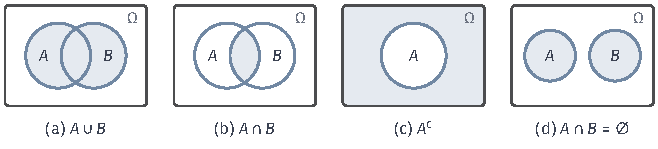
\includegraphics[width=112mm]{figures/07-probability/01-elementary-probability/tikz/cprob-event-operations/figure.pdf}
  \caption{事件的运算。矩形是样本空间$\Omega$，圆是事件，浅蓝区域是运算得到的事件。(a)并；(b)交；(c)补；(d)两个没有公共结果的事件。}
  \label{fig:cprob-event-operations}
\end{BookInlineFigure}

若$A\cap B=\varnothing$，即$A$与$B$没有公共的结果，就称它们\term{互斥}（mutually exclusive），如图~\ref{fig:cprob-event-operations}(d)。互斥的事件不能在同一次试验中同时发生。掷骰时“出现偶数点”与“出现$1$点”互斥；“出现偶数点”与“点数大于$4$”不互斥，结果$6$同时属于二者。

\paragraph{记录方式决定样本空间}
同一个物理过程可以用不同的方式记录，记录方式不同，样本空间就不同。下面用一个摸球问题说明这一点，本章后面会反复回到它：盒中有$5$个球，编号$1,2,3$的是黑球，编号$4,5$的是白球，搅匀后不放回地依次摸出两个。

第一种记录是按先后写下两个球的编号，结果是有序对$(a,b)$，$a\neq b$。第一个球有$5$种可能，第二个球有$4$种，样本空间有$5\times4=20$个点。第二种记录只写下摸到了哪两个球，不管先后，结果是二元子集$\{a,b\}$，共$\binom52=10$个。第三种只记颜色，结果是“黑黑”“黑白”“白黑”“白白”四种。

图~\ref{fig:cprob-urn-records}把三种样本空间并排画出。事件“两个都是黑球”在三种记录下分别是$6$个有序对、$3$个子集和$1$个颜色记录。三种记录描述的是同一件事，但样本点的个数不同，样本点所代表的情形也不同：一个颜色记录“黑黑”合并了$6$个有序对。

\begin{BookInlineFigure}
  \centering
  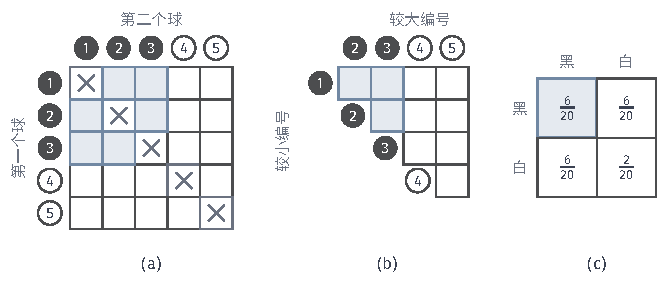
\includegraphics[width=112mm]{figures/07-probability/01-elementary-probability/tikz/cprob-urn-records/figure.pdf}
  \caption{不放回摸两个球的三种记录。实心圆是黑球$1,2,3$，空心圆是白球$4,5$；浅蓝格子是事件“两个都是黑球”。(a)有序对：行是第一个球，列是第二个球，对角线上的格子不可能出现，共$20$个结果。(b)无序对：只保留编号较小者在行、较大者在列的$10$个格子。(c)颜色记录：行、列分别是第一、第二个球的颜色，格中数字是(a)中相应格子数占$20$的比例，四个结果并不同样可能。}
  \label{fig:cprob-urn-records}
\end{BookInlineFigure}

选择样本空间要满足两个要求。第一，它必须细到能表达所关心的事件。事件“第一个球是黑球”在有序记录中是$12$个有序对，在无序记录中却写不出来：子集$\{1,4\}$既可能是先摸到$1$，也可能是先摸到$4$。第二，它最好让每个样本点同样可能，这样概率才能靠计数得到。

颜色记录满足第一个要求，却不满足第二个：图~\ref{fig:cprob-urn-records}(c)中“白白”只对应$2$个有序对，“黑黑”对应$6$个。下一节把“同样可能”写成模型假设，并说明为什么有序记录满足它而颜色记录不满足。

若改为放回摸球，即摸出一个球记下编号后放回盒中，再摸第二个，那么第二个球可以与第一个相同，有序记录的样本空间就是全部$5\times5=25$个有序对，图~\ref{fig:cprob-urn-records}(a)中对角线上的$5$个格子也成为可能结果。放回与否改变的是样本空间本身，而不只是某个事件。

\section{等可能模型}
\label{sec:cprob-equally-likely}

一枚做工均匀的骰子，六个面在形状和重量上没有区别，我们找不到任何理由认为某一面更容易朝上。既然如此，就让六个面分得同样多的可能性，各占$1/6$。“出现偶数点”包含三个面，它的可能性就是$3/6$。把这个想法推广到一般的有限样本空间，就得到用计数定义的概率。

\paragraph{计数比}
可以把概率想成一份总量为$1$的质量，要分配到样本空间的各个点上。等可能就是平均分配：$\Omega$有$\lvert\Omega\rvert$个点，每个点分到$1/\lvert\Omega\rvert$。一个事件的概率，就是落在这个事件区域里的质量总和。点的质量相同，总和就等于点数乘以每点的质量。

\begin{definition}[古典概率]
\label{def:cprob-classical}
设样本空间$\Omega$有限且非空，并假设每个样本点同样可能出现。对每个事件$A\subseteq\Omega$，令
\begin{equation}
 \mathbb{P}(A)=\frac{\lvert A\rvert}{\lvert\Omega\rvert},
 \label{eq:cprob-classical}
\end{equation}
其中$\lvert A\rvert$是$A$的元素个数。称$\mathbb{P}(A)$为事件$A$的概率，称$(\Omega,\mathbb{P})$为\term{古典概率模型}（classical probability model）。
\end{definition}

式~\eqref{eq:cprob-classical}把概率问题完全化成了计数问题：分子数事件里的结果，分母数全部结果，两者都在同一个样本空间里数。每个基本事件的概率都是$1/\lvert\Omega\rvert$，这正是“等可能”的数学表述。

\paragraph{三条基本性质}
这个定义给出的数满足哪些规律？我们希望概率像“占比”一样运算：不会是负数，全体的占比是$1$，两块不重叠的部分合起来，占比相加。下面验证计数比确实具有这三条性质；后面的一切运算规则都从它们推出。

\begin{theorem}[古典概率的基本性质]
\label{thm:cprob-axioms}
在古典概率模型中，对任意事件$A,B$：
\begin{enumerate}
 \item 非负性：
 \begin{equation}
  \mathbb{P}(A)\geq0;
  \label{eq:cprob-nonneg}
 \end{equation}
 \item 归一性：
 \begin{equation}
  \mathbb{P}(\Omega)=1;
  \label{eq:cprob-normalized}
 \end{equation}
 \item 互斥可加性：若$A\cap B=\varnothing$，则
 \begin{equation}
  \mathbb{P}(A\cup B)=\mathbb{P}(A)+\mathbb{P}(B).
  \label{eq:cprob-additive}
 \end{equation}
\end{enumerate}
\end{theorem}

\begin{proof}
元素个数非负，分母$\lvert\Omega\rvert$为正，所以$\mathbb{P}(A)\geq0$。取$A=\Omega$，分子分母相同，比值为$1$。

若$A\cap B=\varnothing$，并集$A\cup B$中的每个元素恰好属于$A$与$B$中的一个，按计数的加法规则
\[
 \lvert A\cup B\rvert=\lvert A\rvert+\lvert B\rvert.
\]
两边同除以$\lvert\Omega\rvert$，就得到式~\eqref{eq:cprob-additive}。
\end{proof}

互斥可加性对有限个两两互斥的事件同样成立。设$A_1,\ldots,A_m$两两互斥，对$m$归纳：$A_1\cup\cdots\cup A_{m-1}$与$A_m$互斥，用一次式~\eqref{eq:cprob-additive}，再用归纳假设，得到
\[
 \mathbb{P}(A_1\cup\cdots\cup A_m)=\mathbb{P}(A_1)+\cdots+\mathbb{P}(A_m).
\]
特别地，任何事件都是它所含基本事件的互斥并，所以$\mathbb{P}(A)$等于$A$中各点概率之和。这与开头“质量总和”的图景一致。

反过来，计数比也是唯一与等可能相容的分配。设某种分配满足三条基本性质，并且每个基本事件的概率都等于同一个数$c$。$\Omega$是它的$\lvert\Omega\rvert$个基本事件的互斥并，由有限可加性与归一性，
\[
 1=\mathbb{P}(\Omega)=\lvert\Omega\rvert\,c,
\]
所以$c=1/\lvert\Omega\rvert$；再对$A$的各点求和，就得到$\mathbb{P}(A)=\lvert A\rvert/\lvert\Omega\rvert$。因此定义~\ref{def:cprob-classical}并没有额外的选择：一旦接受等可能假设和三条性质，概率只能是计数比。

\paragraph{两枚骰子}
掷两枚骰子，把它们看成可区分的第一枚与第二枚，结果记为有序对$(i,j)$，$i,j\in\{1,\ldots,6\}$。样本空间有$36$个点。若每枚骰子都均匀，两次投掷互不干扰，我们就假设这$36$个有序对同样可能。

图~\ref{fig:cprob-dice-grid}把$36$个结果排成方格，格中写的是点数和$i+j$。点数和相同的格子排在同一条斜线上。事件“点数和为$7$”占$6$格，“点数和为$2$”只占$1$格，于是
\[
 \mathbb{P}(\text{点数和为}7)=\frac{6}{36}=\frac16,\qquad
 \mathbb{P}(\text{点数和为}2)=\frac{1}{36}.
\]

\begin{BookInlineFigure}
  \centering
  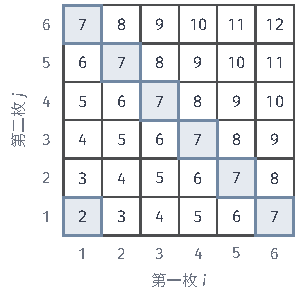
\includegraphics[width=51mm]{figures/07-probability/01-elementary-probability/tikz/cprob-dice-grid/figure.pdf}
  \caption{两枚骰子的$36$个等可能结果。横向是第一枚的点数$i$，纵向是第二枚的点数$j$，格中数字是点数和。浅蓝格子是事件“点数和为$7$”（$6$格）与“点数和为$2$”（$1$格）。}
  \label{fig:cprob-dice-grid}
\end{BookInlineFigure}

点数和从$2$到$12$共$11$种。如果以这$11$个值为样本点，并认为它们同样可能，每个值的概率就都是$1/11$。这与计数结果矛盾：和为$7$的出法有$6$种，和为$2$只有$(1,1)$一种。以点数和为样本点并没有错，错的是对它们使用了等可能假设。

\paragraph{等可能是模型假设}
上面的矛盾说明，式~\eqref{eq:cprob-classical}的前提“每个样本点同样可能”不是从样本空间的写法推出来的，而是对试验所作的假设。它的依据是试验的物理对称性：骰子各面均匀，牌洗得充分，摸球前搅匀且每个球被摸到的机会相同。样本点的名称看起来对称，并不构成这样的依据。

历史上一个有名的错误是这样的：抛两枚硬币，结果分为“两正”“两反”“一正一反”三种，于是认为每种的概率都是$1/3$。按硬币区分先后，等可能的结果是“正正”“正反”“反正”“反反”四种，“一正一反”占了其中两种，所以
\[
 \mathbb{P}(\text{两正})=\frac14,\qquad
 \mathbb{P}(\text{一正一反})=\frac12.
\]
三种结果的名称同样简单，但它们合并的基本结果个数不同，不能平分概率。

哪个模型对，可以用重复试验来检验。把同一试验重复许多次，事件发生的次数除以试验次数称为事件的\term{相对频率}（relative frequency）。图~\ref{fig:cprob-coin-frequency}模拟了$2000$轮抛两枚硬币：随着轮数增加，“两正”的相对频率稳定在$1/4$附近，“一正一反”稳定在$1/2$附近，都远离$1/3$。

\begin{BookInlineFigure}
  \centering
  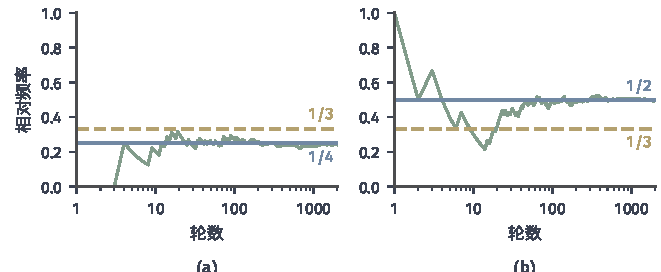
\includegraphics[width=112mm]{figures/07-probability/01-elementary-probability/matplotlib/cprob-coin-frequency/figure.pdf}
  \caption{抛两枚均匀硬币$2000$轮的模拟（随机数种子$3$），横轴为对数坐标。绿线是前若干轮中事件的相对频率，蓝线是四个有序结果等可能时的概率，黄色虚线是错误地认为三种结果等可能时的$1/3$。(a)两正；(b)一正一反。$2000$轮后两个频率分别是$0.2415$和$0.496$。}
  \label{fig:cprob-coin-frequency}
\end{BookInlineFigure}

图~\ref{fig:cprob-dice-sum-frequency}对两枚骰子做了同样的检验。$3600$次模拟中，各点数和的相对频率紧贴计数比$k/36$，其中$k$是该点数和所占的格子数；它们与$1/11$的水平线则明显不符。

\begin{BookInlineFigure}
  \centering
  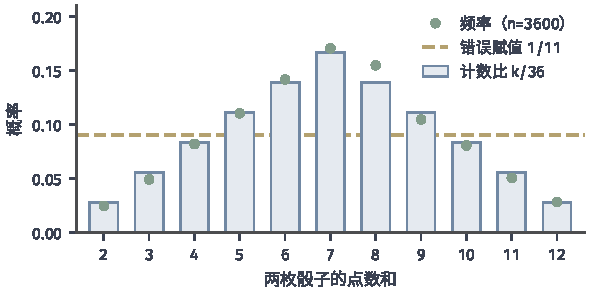
\includegraphics[width=100mm]{figures/07-probability/01-elementary-probability/matplotlib/cprob-dice-sum-frequency/figure.pdf}
  \caption{两枚骰子点数和的概率与频率。浅蓝柱是$36$个有序结果等可能时的概率$k/36$，绿点是$3600$次模拟中的相对频率（随机数种子$7$），黄色虚线是错误地把$11$个点数和看作等可能时的$1/11$。}
  \label{fig:cprob-dice-sum-frequency}
\end{BookInlineFigure}

\paragraph{古典概率与频率}
古典概率和相对频率回答的是不同的问题。古典概率由模型算出，是一个确定的数，不依赖任何实际的投掷；相对频率由观察得到，每做一批试验结果都不同，图~\ref{fig:cprob-coin-frequency}中前几十轮的波动很大。前者是对试验的假设所推出的结论，后者是对试验本身的记录。

两者的联系是：如果模型的等可能假设与试验相符，相对频率在大量重复中会靠近模型给出的概率；如果明显偏离，就说明假设与试验不符，例如一枚灌铅的骰子会让某一面的频率持续偏高。“频率靠近概率”在什么意义下成立，需要先有独立重复试验和随机变量的语言，这一结论在第~\ref{chap:laws-of-large-numbers}章证明。本章只把频率当作检验模型的经验依据，不用它来定义概率。

\paragraph{再看摸球问题}
回到第~\ref{sec:cprob-experiments}节的摸球问题。搅匀后摸球，每个球被第一个摸到的机会相同；摸走一个以后，剩下的四个球被第二个摸到的机会也相同。所以$20$个有序对同样可能，有序记录满足等可能假设。

在有序记录中，“两个都是黑球”有$3\times2=6$个结果，“第一个黑、第二个白”有$3\times2=6$个，“第一个白、第二个黑”有$2\times3=6$个，“两个都是白球”有$2\times1=2$个。于是四个颜色记录的概率分别是
\[
 \frac{6}{20},\quad \frac{6}{20},\quad \frac{6}{20},\quad \frac{2}{20}.
\]
这就是图~\ref{fig:cprob-urn-records}(c)中的数。颜色记录可以作为样本空间，但它的四个点不等可能，不能用计数比；它们的概率要从有序记录算出。第~\ref{sec:cprob-scope}节会专门讨论这种合并带来的问题。

\section{事件概率的计算}
\label{sec:cprob-computing}

有了式~\eqref{eq:cprob-classical}，计算概率就是数两个集合。真正的困难在于数对：样本空间要选得等可能，事件要在同一个样本空间里数，补、并、交这些组合事件要用合适的方式拆开。本节先整理抽样问题中常用的计数公式，再分别处理补事件、并事件和交事件。

\paragraph{四种抽样方式}
从$n$个可区分的对象中取$k$次，按“是否放回”和“是否记录次序”可以分成四种情形。各自的结果个数在\BookChapterRef{chap:counting}{卷一第2章“计数”}中已经得到，记$P(n,k)=n(n-1)\cdots(n-k+1)$为排列数，$\binom nk$为组合数。表~\ref{tab:cprob-sampling}把它们放在一起，并标出每种记录下的结果是否同样可能。

\begin{BookInlineTable}
  \centering
  \caption{从$n$个对象中取$k$次的四种记录方式}
  \label{tab:cprob-sampling}
  \begin{tabular}{llll}
    \toprule
    记录方式 & 结果的形式 & 结果个数 & 是否等可能 \\
    \midrule
    不放回、有序 & 无重复的$k$元有序组 & $P(n,k)$ & 是 \\
    不放回、无序 & $k$元子集 & $\binom nk$ & 是 \\
    放回、有序 & 可重复的$k$元有序组 & $n^{k}$ & 是 \\
    放回、无序 & 可重复的$k$元组合 & $\binom{n+k-1}{k}$ & 否 \\
    \bottomrule
  \end{tabular}
\end{BookInlineTable}

前三种的等可能性来自同一个物理假设：每次取样时，剩下的各对象被取到的机会相同。有序记录直接继承这一假设。不放回的无序记录中，每个$k$元子集恰好由$k!$个有序组忘去次序得到，各子集合并的有序组个数相同，所以仍等可能。放回的无序记录则不然：取两次时，组合$\{1,1\}$只来自有序组$(1,1)$，组合$\{1,2\}$却来自$(1,2)$和$(2,1)$两个。这一行不能直接用于计数比，第~\ref{sec:cprob-scope}节再回到它。

\paragraph{分子与分母同一口径}
在摸球问题中计算“两个都是黑球”的概率。用有序记录，分母是$P(5,2)=20$，分子是从$3$个黑球中有序地取$2$个，$P(3,2)=6$；用无序记录，分母是$\binom52=10$，分子是$\binom32=3$。两种算法给出
\[
 \frac{P(3,2)}{P(5,2)}=\frac{6}{20}=\frac{3}{10},\qquad
 \frac{\binom32}{\binom52}=\frac{3}{10}.
\]
结果一致。若分子用无序的$3$、分母用有序的$20$，就得到$3/20$，这个数不是任何事件的概率。

两种口径给出同一结果并非巧合。“两个都是黑球”只关心摸到了哪些球，不关心先后。对这样的事件，每个满足条件的子集恰好对应$k!$个满足条件的有序组，分子和分母同乘以$k!$，比值不变。这个论证也说明了口径一致的含义：分子和分母必须是同一个样本空间中的计数。

事件“恰好一个黑球”同样只与内容有关。无序记录中它有$3\times2=6$个子集，有序记录中有$3\times2\times2=12$个有序对，概率都是$3/5$。事件“第一个是黑球”则与次序有关，只能在有序记录中数：第一个位置有$3$种，第二个位置从剩下$4$个中任取，共$12$个，概率也是$3/5$。

\paragraph{一副牌中的组合计数}
从一副$52$张的扑克牌中随机抽$3$张，不放回。每个$3$张的子集同样可能。事件“$3$张都是红桃”要求$3$张全部取自$13$张红桃，所以
\[
 \mathbb{P}(\text{三张都是红桃})=\frac{\binom{13}{3}}{\binom{52}{3}}
 =\frac{286}{22100}=\frac{11}{850}\approx0.0129.
\]
第~\ref{sec:cprob-conditional}节会用逐张抽取的方式重新得到这个数。

事件较复杂时，常把满足条件的结果拆成几步来构造，再用乘法规则计数。这时要检查两件事：每一步的选择合起来恰好得到事件中的一个结果，事件中的每个结果也只由一种选择方式得到。以抽$5$张牌“恰好一对”为例，它要求有两张点数相同，其余三张的点数互不相同，也都不同于这一对。

按下面的步骤构造：先选成对的点数，有$13$种；再选这一对的两种花色，有$\binom42=6$种；再从其余$12$个点数中选出三个单张的点数，有$\binom{12}{3}=220$种；最后给三个单张各选一种花色，有$4^{3}=64$种。每手“恰好一对”的牌由唯一一组选择得到，所以
\[
 \mathbb{P}(\text{恰好一对})=\frac{13\times6\times220\times64}{\binom{52}{5}}
 =\frac{1098240}{2598960}\approx0.4226.
\]

一种常见的错误算法是：选好一对之后，从剩下的$48$张牌中任取$3$张，得到$13\times6\times\binom{48}{3}$。这样取出的三张可能又凑成一对，或与已选的一对同点数，于是两对、三条等牌型也被算了进去，而且一手两对的牌按“哪一对先选”会被数两次。另一种错误是把三个单张的点数按$12\times11\times10$有序地选，每手牌被重复数了$3!$次。两种错误都破坏了“恰好一个结果对应一种选择”。

\paragraph{补事件}
“至少一个”“不全相同”这类事件往往由许多情形组成，直接数很麻烦，它的反面却只有一种或少数几种情形。下面的公式把概率转到补事件上。

\begin{theorem}[补事件与包含关系]
\label{thm:cprob-complement}
在古典概率模型中，对任意事件$A$，
\begin{equation}
 \mathbb{P}(A^{\mathrm{c}})=1-\mathbb{P}(A).
 \label{eq:cprob-complement}
\end{equation}
若$A\subseteq B$，则
\begin{equation}
 \mathbb{P}(B\setminus A)=\mathbb{P}(B)-\mathbb{P}(A),\qquad
 \mathbb{P}(A)\leq\mathbb{P}(B)\leq1.
 \label{eq:cprob-monotone}
\end{equation}
特别地，$\mathbb{P}(\varnothing)=0$。
\end{theorem}

\begin{proof}
若$A\subseteq B$，则$B$是互斥的$A$与$B\setminus A$之并。由互斥可加性~\eqref{eq:cprob-additive}，
\[
 \mathbb{P}(B)=\mathbb{P}(A)+\mathbb{P}(B\setminus A).
\]
移项得到式~\eqref{eq:cprob-monotone}的等式；由非负性~\eqref{eq:cprob-nonneg}，$\mathbb{P}(B\setminus A)\geq0$，所以$\mathbb{P}(A)\leq\mathbb{P}(B)$。取$B=\Omega$，用归一性~\eqref{eq:cprob-normalized}，就得到式~\eqref{eq:cprob-complement}与$\mathbb{P}(B)\leq1$。再取$A=\Omega$，得到$\mathbb{P}(\varnothing)=1-1=0$。
\end{proof}

证明只用了三条基本性质，没有再回到计数。这一点后面很重要：凡是满足这三条性质的概率分配，补事件公式都成立。

\paragraph{生日问题}
一个班有$n$个人，至少两人同一天生日的概率是多少？作模型假设：一年按$365$天计，每人的生日在$365$天中等可能，各人之间互不影响。依次写下$n$个人的生日，结果是可重复的有序组，样本空间有$365^{n}$个等可能的点。

“至少两人同一天”包含两人相同、三人相同、两对分别相同等许多情形；它的补事件“$n$个生日两两不同”只有一种情形，正是不放回的有序取法，共$P(365,n)$个。由式~\eqref{eq:cprob-complement}，
\begin{equation}
 \mathbb{P}(\text{至少两人同一天生日})
 =1-\frac{P(365,n)}{365^{n}}
 =1-\prod_{i=0}^{n-1}\Bigl(1-\frac{i}{365}\Bigr).
 \label{eq:cprob-birthday}
\end{equation}

代入$n=23$，乘积约为$0.4927$，所求概率约为$0.5073$，已经超过一半；$n=50$时约为$0.970$。图~\ref{fig:cprob-birthday}画出了它随$n$的变化。这个结果常常出人意料，原因在于要比较的是人与人之间的配对，$23$个人之间有$\binom{23}{2}=253$对，每一对都可能撞上。

\begin{BookInlineFigure}
  \centering
  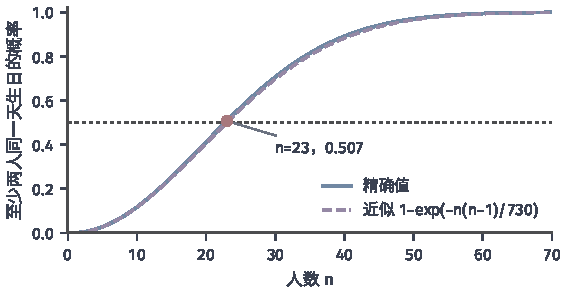
\includegraphics[width=96mm]{figures/07-probability/01-elementary-probability/matplotlib/cprob-birthday/figure.pdf}
  \caption{生日问题。蓝线是式~\eqref{eq:cprob-birthday}的精确值，紫色虚线是近似$1-\exp(-n(n-1)/730)$，黑色点线是$1/2$；红点标出$n=23$时的$0.507$。}
  \label{fig:cprob-birthday}
\end{BookInlineFigure}

配对的说法可以变成一个不等式。由$1-x\leq\mathrm{e}^{-x}$对所有实数$x$成立，乘积中每个因子都不超过$\mathrm{e}^{-i/365}$；$n\leq365$时各因子非负，不等式可以逐项相乘，于是
\[
 \prod_{i=0}^{n-1}\Bigl(1-\frac{i}{365}\Bigr)
 \leq\exp\Bigl(-\sum_{i=0}^{n-1}\frac{i}{365}\Bigr)
 =\exp\Bigl(-\frac{n(n-1)}{730}\Bigr).
\]
指数中的$n(n-1)/2$正是配对数。$n=23$时右端为$\mathrm{e}^{-506/730}\approx0.499998$，略小于$1/2$，所以不需要计算乘积，就知道所求概率大于$1/2$。图中紫色虚线与蓝线几乎重合，说明$i/365$较小时这个上界也很接近真实值。

\paragraph{并事件}
两个事件的并，直接相加会出错：$\lvert A\rvert+\lvert B\rvert$把$A\cap B$中的结果数了两次。减去重复的部分，就是计数的容斥原理在概率中的形式。

\begin{theorem}[加法公式]
\label{thm:cprob-addition}
在古典概率模型中，对任意事件$A,B$，
\begin{equation}
 \mathbb{P}(A\cup B)=\mathbb{P}(A)+\mathbb{P}(B)-\mathbb{P}(A\cap B).
 \label{eq:cprob-addition}
\end{equation}
对三个事件$A,B,C$，
\begin{equation}
 \begin{aligned}
 \mathbb{P}(A\cup B\cup C)
 &=\mathbb{P}(A)+\mathbb{P}(B)+\mathbb{P}(C)\\
 &\quad-\mathbb{P}(A\cap B)-\mathbb{P}(A\cap C)-\mathbb{P}(B\cap C)\\
 &\quad+\mathbb{P}(A\cap B\cap C).
 \end{aligned}
 \label{eq:cprob-inclusion-exclusion}
\end{equation}
\end{theorem}

\begin{proof}
$A\cup B$可以拆成互斥的三块$A\setminus B$、$A\cap B$、$B\setminus A$；$A$是前两块之并，$B$是后两块之并。由互斥可加性~\eqref{eq:cprob-additive}，
\[
 \begin{aligned}
 \mathbb{P}(A\cup B)&=\mathbb{P}(A\setminus B)+\mathbb{P}(A\cap B)+\mathbb{P}(B\setminus A),\\
 \mathbb{P}(A)+\mathbb{P}(B)&=\mathbb{P}(A\setminus B)+2\,\mathbb{P}(A\cap B)+\mathbb{P}(B\setminus A).
 \end{aligned}
\]
两式相减即得式~\eqref{eq:cprob-addition}。

对三个事件，把$B\cup C$看成一个事件，先用一次式~\eqref{eq:cprob-addition}：
\[
 \mathbb{P}(A\cup B\cup C)=\mathbb{P}(A)+\mathbb{P}(B\cup C)-\mathbb{P}\bigl((A\cap B)\cup(A\cap C)\bigr).
\]
再对$\mathbb{P}(B\cup C)$和最后一项各用一次式~\eqref{eq:cprob-addition}，注意$(A\cap B)\cap(A\cap C)=A\cap B\cap C$，整理即得式~\eqref{eq:cprob-inclusion-exclusion}。
\end{proof}

对$m$个事件，同样的公式在交替加减所有$k$个事件之交的概率后成立，它是有限容斥原理两边同除以$\lvert\Omega\rvert$的结果。丢掉式~\eqref{eq:cprob-addition}中非负的一项$\mathbb{P}(A\cap B)$，得到
\begin{equation}
 \mathbb{P}(A\cup B)\leq\mathbb{P}(A)+\mathbb{P}(B),
 \label{eq:cprob-union-bound}
\end{equation}
对事件个数归纳可推广到任意有限个事件，称为\term{联合界}（union bound）。它不要求事件之间有任何关系，常用来估计“至少一处出问题”的概率。

\paragraph{至少一个六点}
掷两枚骰子，求至少出现一个六点的概率。令$A$为“第一枚是六点”，$B$为“第二枚是六点”，所求事件是$A\cup B$。$A$与$B$各占$6$格，它们只在$(6,6)$这一格重叠，如图~\ref{fig:cprob-at-least-one-six}(a)所示。由式~\eqref{eq:cprob-addition}，
\[
 \mathbb{P}(A\cup B)=\frac{6}{36}+\frac{6}{36}-\frac{1}{36}=\frac{11}{36}.
\]

\begin{BookInlineFigure}
  \centering
  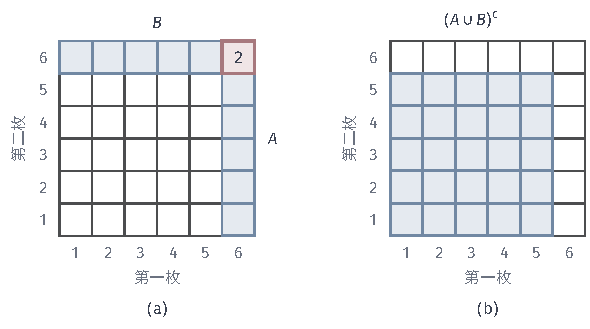
\includegraphics[width=100mm]{figures/07-probability/01-elementary-probability/tikz/cprob-at-least-one-six/figure.pdf}
  \caption{两枚骰子中至少一个六点。(a)浅蓝的一列是$A$（第一枚六点），浅蓝的一行是$B$（第二枚六点），红格$(6,6)$在$\lvert A\rvert+\lvert B\rvert$中被数了两次。(b)补事件“两枚都不是六点”是$5\times5$的方块。}
  \label{fig:cprob-at-least-one-six}
\end{BookInlineFigure}

用补事件计算更直接。由De Morgan律，$(A\cup B)^{\mathrm{c}}$就是$A^{\mathrm{c}}\cap B^{\mathrm{c}}$，即“两枚都不是六点”，即图~\ref{fig:cprob-at-least-one-six}(b)中$5\times5=25$个格子，所以概率是$1-25/36=11/36$，两种算法一致。

掷三枚骰子时两种方法的差别更明显。用式~\eqref{eq:cprob-inclusion-exclusion}，单个事件各占$36$个结果，两两之交各占$6$个，三者之交占$1$个，于是
\[
 \mathbb{P}(\text{至少一个六点})=\frac{3\times36-3\times6+1}{216}=\frac{91}{216}.
\]
用补事件，“三枚都不是六点”有$5^{3}=125$个结果，概率是$1-125/216=91/216$。补事件只需要一次计数，容斥原理需要逐层修正。

\paragraph{交事件}
交事件要求几个条件同时满足，一般要在样本空间中把两个条件一起数。在摸球问题的有序记录中，令$H_1$为“第一个是黑球”，$E$为“两个球颜色不同”。$H_1\cap E$就是“第一个黑、第二个白”，有$3\times2=6$个有序对，所以$\mathbb{P}(H_1\cap E)=6/20$。

此时$\mathbb{P}(H_1)=12/20$，$\mathbb{P}(E)=12/20$，二者相乘得$0.36$，并不等于$0.3$。交事件的概率一般不能由各自的概率相乘得到；什么时候可以相乘，是第~\ref{sec:cprob-independence}节的问题。

\paragraph{放回与不放回}
最后固定一个抽检问题，比较放回与不放回。一批$20$件产品中有$4$件次品，随机抽取$5$件检查。不放回时，每个$5$件子集等可能，“没有次品”要求$5$件都取自$16$件合格品：
\[
 \mathbb{P}_{\text{不放回}}(\text{没有次品})=\frac{\binom{16}{5}}{\binom{20}{5}}=\frac{4368}{15504}\approx0.2817.
\]
若改用不放回的有序记录，分子分母分别是$P(16,5)$和$P(20,5)$，比值不变。

放回时，每次都从全部$20$件中取，有序记录有$20^{5}$个等可能结果，其中每次都取到合格品的有$16^{5}$个：
\[
 \mathbb{P}_{\text{放回}}(\text{没有次品})=\Bigl(\frac{16}{20}\Bigr)^{5}=0.32768.
\]
放回时同一件合格品可以被反复抽到，合格品“用不完”，所以全是合格品的机会更大。

两种方式下“恰好一件次品”的计数方法不同。不放回时选$1$件次品、$4$件合格品，概率为
\[
 \frac{\binom41\binom{16}{4}}{\binom{20}{5}}=\frac{7280}{15504}\approx0.4696.
\]
放回时必须用有序记录：先选次品出现在哪一次，有$5$种；该次有$4$种取法，其余四次各有$16$种。于是概率为
\[
 \frac{5\times4\times16^{4}}{20^{5}}=0.4096.
\]
这里不能把放回的结果按无序组合来数，因为表~\ref{tab:cprob-sampling}最后一行的结果不等可能。

图~\ref{fig:cprob-replacement-compare}把“没有次品”的概率画成抽取件数$k$的函数。不放回的曲线始终低于放回的曲线，并在$k=17$时降到$0$：$17$件中至少有一件次品，因为合格品只有$16$件。$k$相对于$20$较小时两条曲线很接近，每次抽走一件对剩余构成的影响较小。

\begin{BookInlineFigure}
  \centering
  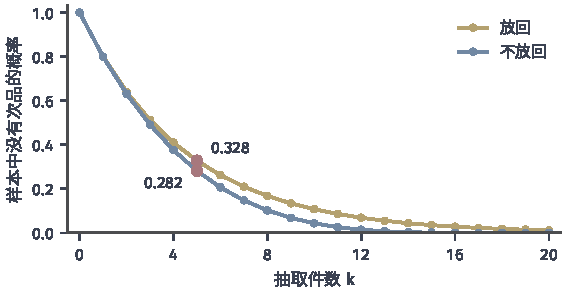
\includegraphics[width=96mm]{figures/07-probability/01-elementary-probability/matplotlib/cprob-replacement-compare/figure.pdf}
  \caption{$20$件中含$4$件次品时，抽取$k$件都是合格品的概率。蓝线是不放回抽样$\binom{16}{k}/\binom{20}{k}$，黄线是放回抽样$0.8^{k}$；红点标出正文中$k=5$的两个值。}
  \label{fig:cprob-replacement-compare}
\end{BookInlineFigure}

\section{条件概率}
\label{sec:cprob-conditional}

掷两枚骰子，第一枚是六点的概率是$1/6$。若有人看了一眼，告诉我们“点数和不小于$9$”，第一枚是六点的可能性还是$1/6$吗？直觉上应该更大，点数和大，说明骰子点数偏高。已知信息排除了一部分结果，剩余不确定性应当只在留下的结果中描述。

\paragraph{缩小范围，重新归一}
令$A$为“第一枚是六点”，$B$为“点数和不小于$9$”。$B$包含点数和为$9,10,11,12$的格子，个数分别是$4,3,2,1$，共$10$个；其中第一枚是六点的有$(6,3),(6,4),(6,5),(6,6)$这$4$个，如图~\ref{fig:cprob-conditioning-shrink}所示。

既然知道结果落在$B$中，$B$之外的$26$个格子就不必再考虑。原来$36$个结果等可能，留下的$10$个结果之间也没有理由偏向哪个，所以把它们看成新的等可能样本空间，每格的概率从$1/36$变为$1/10$。在这个缩小的范围里，$A$占$4$格，可能性是$4/10=2/5$。

\begin{BookInlineFigure}
  \centering
  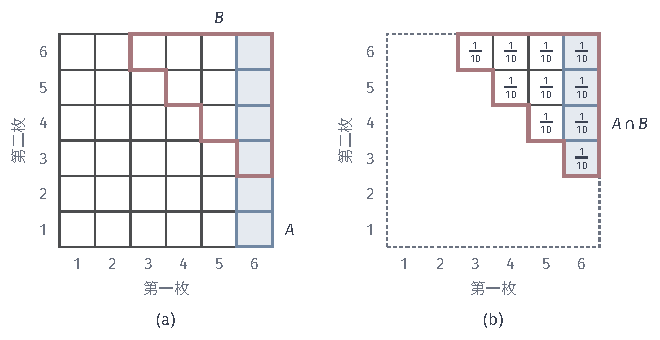
\includegraphics[width=112mm]{figures/07-probability/01-elementary-probability/tikz/cprob-conditioning-shrink/figure.pdf}
  \caption{以“点数和不小于$9$”为条件。(a)红线围出条件事件$B$的$10$个格子，浅蓝一列是$A$（第一枚六点），每格概率$1/36$。(b)只保留$B$中的格子，每格重新分得$1/10$；浅蓝格子是$A\cap B$，共$4$格，条件概率为$4/10$。}
  \label{fig:cprob-conditioning-shrink}
\end{BookInlineFigure}

把这个计算写成概率的形式。在古典模型中，
\[
 \frac{\lvert A\cap B\rvert}{\lvert B\rvert}
 =\frac{\lvert A\cap B\rvert/\lvert\Omega\rvert}{\lvert B\rvert/\lvert\Omega\rvert}
 =\frac{\mathbb{P}(A\cap B)}{\mathbb{P}(B)}.
\]
右端不再提到计数，只用到事件的概率，因此可以作为一般的定义。

\begin{definition}[条件概率]
\label{def:cprob-conditional}
设事件$B$满足$\mathbb{P}(B)>0$。事件$A$在$B$发生条件下的\term{条件概率}（conditional probability）定义为
\begin{equation}
 \mathbb{P}(A\mid B)=\frac{\mathbb{P}(A\cap B)}{\mathbb{P}(B)}.
 \label{eq:cprob-conditional}
\end{equation}
\end{definition}

分子只保留$A$中同时落在$B$内的部分，分母把$B$的概率重新标定为$1$。用质量的图景说：把$B$之外的质量全部清除，再把$B$内的质量按原有比例放大，使总量回到$1$。$B$内各点之间的相对大小不变，这正是“已知$B$发生”所允许的全部修改。

条件$\mathbb{P}(B)>0$不能去掉。在有限的古典模型中，$\mathbb{P}(B)=0$意味着$B=\varnothing$，以一个不可能发生的事件为条件没有意义，式~\eqref{eq:cprob-conditional}的分母也为零。

\paragraph{条件概率仍是概率}
固定$B$以后，$A\mapsto\mathbb{P}(A\mid B)$给每个事件分配了一个数。它满足前面的三条基本性质，因而第~\ref{sec:cprob-computing}节的补事件公式、加法公式在条件之下都可以照用。

\begin{theorem}[条件概率的基本性质]
\label{thm:cprob-conditional-axioms}
设$\mathbb{P}(B)>0$，则对任意事件$A,A'$，
\begin{equation}
 \mathbb{P}(A\mid B)\geq0,\qquad \mathbb{P}(\Omega\mid B)=1,
 \label{eq:cprob-conditional-normalized}
\end{equation}
并且当$A\cap A'=\varnothing$时，
\begin{equation}
 \mathbb{P}(A\cup A'\mid B)=\mathbb{P}(A\mid B)+\mathbb{P}(A'\mid B).
 \label{eq:cprob-conditional-additive}
\end{equation}
\end{theorem}

\begin{proof}
非负性来自分子非负、分母为正。由$\Omega\cap B=B$，分子分母相同，所以$\mathbb{P}(\Omega\mid B)=1$。若$A\cap A'=\varnothing$，则$A\cap B$与$A'\cap B$也互斥，且它们的并是$(A\cup A')\cap B$。由式~\eqref{eq:cprob-additive}，
\[
 \mathbb{P}\bigl((A\cup A')\cap B\bigr)=\mathbb{P}(A\cap B)+\mathbb{P}(A'\cap B).
\]
两边同除以$\mathbb{P}(B)$，就得到式~\eqref{eq:cprob-conditional-additive}。
\end{proof}

例如在上面的骰子例子中，$\mathbb{P}(A^{\mathrm{c}}\mid B)=1-2/5=3/5$，即已知点数和不小于$9$时，第一枚不是六点的概率是$3/5$。

\paragraph{两个方向的条件概率}
$\mathbb{P}(A\mid B)$与$\mathbb{P}(B\mid A)$的分子相同，都是$\mathbb{P}(A\cap B)$，分母不同。在骰子例子中，
\[
 \mathbb{P}(A\mid B)=\frac{4/36}{10/36}=\frac25,\qquad
 \mathbb{P}(B\mid A)=\frac{4/36}{6/36}=\frac23.
\]
前者是“点数和大时，第一枚是六点的概率”，后者是“第一枚是六点时，点数和大的概率”。它们回答不同的问题，一般不相等。把两者混为一谈是条件概率中最常见的错误，后面的检测例子会显示它可以造成多大的偏差。

已知$B$让$A$的概率从$1/6$升到$2/5$，这是信息的作用。条件概率也可能比原概率小，例如已知“点数和不大于$4$”时，第一枚是六点的概率降为$0$。若条件概率与原概率相等，条件就没有改变$A$的可能性，这种情形在第~\ref{sec:cprob-independence}节研究。

\subsection{乘法规则}
\label{sec:cprob-multiplication-rule}

很多试验是分步进行的：先摸第一个球，再摸第二个；先选产线，再看产品是否合格。每一步的条件概率往往可以直接从当时的物理状态读出，而整个样本空间却不必列出。把定义~\eqref{eq:cprob-conditional}反过来用，就能把这些逐步的概率乘起来。

\paragraph{两步乘法}
式~\eqref{eq:cprob-conditional}两边乘以$\mathbb{P}(B)$，得到
\begin{equation}
 \mathbb{P}(A\cap B)=\mathbb{P}(B)\,\mathbb{P}(A\mid B),\qquad \mathbb{P}(B)>0.
 \label{eq:cprob-multiplication}
\end{equation}
这称为概率的\term{乘法规则}（multiplication rule）。它的含义是比例的比例：$B$占全体的比例，乘以$A$在$B$内部所占的比例，等于$A\cap B$占全体的比例。

回到摸球问题，令$H_i$为“第$i$个球是黑球”。第一个球是黑球的概率是$3/5$。第一个黑球摸走以后，盒中剩下$2$黑$2$白，所以$\mathbb{P}(H_2\mid H_1)=2/4$。由式~\eqref{eq:cprob-multiplication}，
\[
 \mathbb{P}(H_1\cap H_2)=\mathbb{P}(H_1)\,\mathbb{P}(H_2\mid H_1)=\frac35\cdot\frac24=\frac{3}{10}.
\]
这与第~\ref{sec:cprob-computing}节在有序记录中数出的$6/20$一致。

这里的$\mathbb{P}(H_2\mid H_1)=2/4$是从“已知第一个是黑球”这个条件下盒中的实际构成读出来的。若忽略条件的变化，把第二步也写成$3/5$，就会得到$9/25$，那是放回摸球的答案。不放回抽样中，每一步的条件概率都必须对应前面已经发生的结果。

\paragraph{树形图}
把所有分步的情形画出来，就得到图~\ref{fig:cprob-urn-tree}的树形图。从根出发，每一层是一步，分支上写的是在到达该分支之前的结果已知时的条件概率；从根到叶的一条路径是一个完整的结果，它的概率是路径上各分支概率的乘积。

\begin{BookInlineFigure}
  \centering
  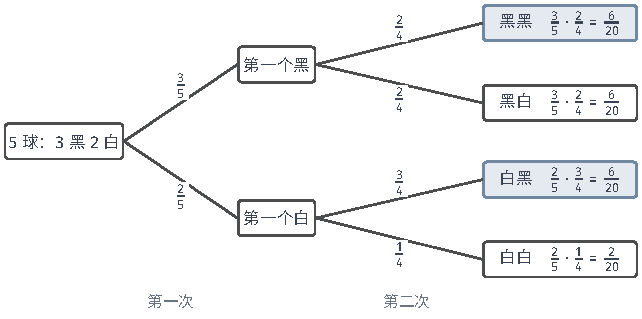
\includegraphics[width=109mm]{figures/07-probability/01-elementary-probability/tikz/cprob-urn-tree/figure.pdf}
  \caption{不放回摸两个球的树形图（盒中$3$黑$2$白）。分支上的数是条件概率，叶上是路径概率的乘积；四个叶的概率之和为$1$。浅蓝的两个叶组成事件$H_2$“第二个是黑球”。}
  \label{fig:cprob-urn-tree}
\end{BookInlineFigure}

同一个节点引出的分支，条件概率之和为$1$，这是式~\eqref{eq:cprob-conditional-normalized}的体现；因此全部叶的概率之和也是$1$。树形图上的叶就是颜色记录的四个结果，叶上的数与图~\ref{fig:cprob-urn-records}(c)一致。

\paragraph{多步乘法}
步骤更多时，反复使用式~\eqref{eq:cprob-multiplication}即可。

\begin{theorem}[多步乘法规则]
\label{thm:cprob-chain-rule}
设事件$A_1,\ldots,A_n$满足$\mathbb{P}(A_1\cap\cdots\cap A_{n-1})>0$，则
\begin{equation}
 \mathbb{P}(A_1\cap\cdots\cap A_n)
 =\mathbb{P}(A_1)\prod_{k=2}^{n}\mathbb{P}(A_k\mid A_1\cap\cdots\cap A_{k-1}).
 \label{eq:cprob-chain-rule}
\end{equation}
\end{theorem}

\begin{proof}
记$C_k=A_1\cap\cdots\cap A_k$。由包含关系$C_{n-1}\subseteq C_{n-2}\subseteq\cdots\subseteq C_1$与式~\eqref{eq:cprob-monotone}，各$\mathbb{P}(C_k)\geq\mathbb{P}(C_{n-1})>0$，右端每个条件概率都有定义。由定义~\eqref{eq:cprob-conditional}与$C_{k-1}\cap A_k=C_k$，
\[
 \mathbb{P}(A_k\mid C_{k-1})=\frac{\mathbb{P}(C_k)}{\mathbb{P}(C_{k-1})},\qquad k=2,\ldots,n,
\]
所以右端是
\[
 \mathbb{P}(C_1)\cdot\frac{\mathbb{P}(C_2)}{\mathbb{P}(C_1)}\cdot\frac{\mathbb{P}(C_3)}{\mathbb{P}(C_2)}\cdots\frac{\mathbb{P}(C_n)}{\mathbb{P}(C_{n-1})}.
\]
相邻的分子分母逐个相消，只剩$\mathbb{P}(C_n)$，即左端。
\end{proof}

用它重新计算第~\ref{sec:cprob-computing}节的扑克牌问题。令$R_k$为“第$k$张是红桃”。第一张是红桃的概率是$13/52$；已知第一张是红桃，剩下$51$张中有$12$张红桃；已知前两张都是红桃，剩下$50$张中有$11$张。由式~\eqref{eq:cprob-chain-rule}，
\[
 \mathbb{P}(R_1\cap R_2\cap R_3)=\frac{13}{52}\cdot\frac{12}{51}\cdot\frac{11}{50}=\frac{1716}{132600}=\frac{11}{850}.
\]
这与组合计数$\binom{13}{3}/\binom{52}{3}$的结果相同。组合计数一次数完整个样本空间，乘法规则则沿抽取过程逐步计算，每一步只需看当时剩下什么。

\subsection{全概率与Bayes公式}
\label{sec:cprob-total-bayes}

一家工厂有甲、乙、丙三条产线，某天生产的$1000$件产品中，甲线$500$件、乙线$300$件、丙线$200$件，次品分别有$10$件、$12$件、$20$件。从这$1000$件中随机抽一件，它是次品的概率是多少？如果它是次品，它最可能来自哪条产线？前一个问题按来源分组再合计，后一个问题从结果反推来源。

\paragraph{按情形分组}
令$L_1,L_2,L_3$分别为“抽到的产品来自甲、乙、丙线”，$D$为“抽到的是次品”。每件产品恰好来自一条产线，所以$L_1,L_2,L_3$两两互斥，并且它们的并是$\Omega$。这样一组事件称为样本空间的一个\term{划分}（partition）：每次试验中恰有一个$L_i$发生。

每条产线的比例和次品率可以直接读出：
\[
 \mathbb{P}(L_1)=0.5,\quad \mathbb{P}(L_2)=0.3,\quad \mathbb{P}(L_3)=0.2,
\]
\[
 \mathbb{P}(D\mid L_1)=\frac{10}{500}=0.02,\qquad
 \mathbb{P}(D\mid L_2)=\frac{12}{300}=0.04,
\]
\[
 \mathbb{P}(D\mid L_3)=\frac{20}{200}=0.10.
\]
要得到$\mathbb{P}(D)$，把$D$按来源切成三块，分别用乘法规则计算，再相加。

\begin{theorem}[全概率公式]
\label{thm:cprob-total-probability}
设$L_1,\ldots,L_m$是样本空间的一个划分，且每个$\mathbb{P}(L_i)>0$。则对任意事件$D$，
\begin{equation}
 \mathbb{P}(D)=\sum_{i=1}^{m}\mathbb{P}(L_i)\,\mathbb{P}(D\mid L_i).
 \label{eq:cprob-total-probability}
\end{equation}
\end{theorem}

\begin{proof}
由$L_1\cup\cdots\cup L_m=\Omega$，得$D=(D\cap L_1)\cup\cdots\cup(D\cap L_m)$；由$L_i$两两互斥，各块$D\cap L_i$也两两互斥。由有限个事件的互斥可加性，
\[
 \mathbb{P}(D)=\sum_{i=1}^{m}\mathbb{P}(D\cap L_i).
\]
对每一项用乘法规则~\eqref{eq:cprob-multiplication}，把$\mathbb{P}(D\cap L_i)$写成$\mathbb{P}(L_i)\mathbb{P}(D\mid L_i)$，代入即得。
\end{proof}

式~\eqref{eq:cprob-total-probability}称为\term{全概率公式}（law of total probability）。它是一个加权平均：各组的次品率$\mathbb{P}(D\mid L_i)$按各组所占的比例$\mathbb{P}(L_i)$加权。代入产线的数据，
\[
 \mathbb{P}(D)=0.5\times0.02+0.3\times0.04+0.2\times0.10=0.010+0.012+0.020=0.042.
\]
这正是$1000$件中次品所占的比例$42/1000$。

图~\ref{fig:cprob-line-mosaic}(a)把这个加权平均画成面积。单位正方形按产线比例分成三列，每列底部深色条的高度是该线的次品率，深色条的面积就是$\mathbb{P}(D\cap L_i)$，三块面积之和是$\mathbb{P}(D)$。

\begin{BookInlineFigure}
  \centering
  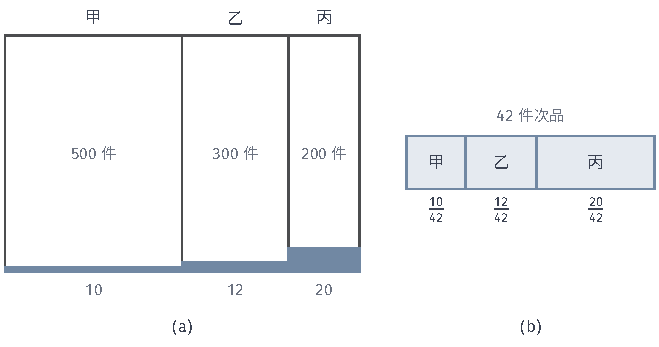
\includegraphics[width=112mm]{figures/07-probability/01-elementary-probability/tikz/cprob-line-mosaic/figure.pdf}
  \caption{三条产线的面积图，按真实比例绘制。(a)列宽是产线所占比例$0.5,0.3,0.2$，底部深蓝条的高度是次品率$0.02,0.04,0.10$，下方数字是各线次品件数；深蓝条的总面积是$\mathbb{P}(D)=0.042$。(b)只看$42$件次品，每件占同样长度，三段的比例就是$\mathbb{P}(L_i\mid D)$。}
  \label{fig:cprob-line-mosaic}
\end{BookInlineFigure}

\paragraph{从结果反推来源}
现在已知抽到的是次品，问它来自各条产线的概率。按定义，这是把范围缩小到$D$，在其中计算$L_i\cap D$所占的比例。分子用乘法规则写开，分母用全概率公式写开，就得到下面的公式。

\begin{theorem}[Bayes公式]
\label{thm:cprob-bayes}
在定理~\ref{thm:cprob-total-probability}的条件下，若$\mathbb{P}(D)>0$，则对每个$i$，
\begin{equation}
 \mathbb{P}(L_i\mid D)=\frac{\mathbb{P}(L_i)\,\mathbb{P}(D\mid L_i)}{\sum_{j=1}^{m}\mathbb{P}(L_j)\,\mathbb{P}(D\mid L_j)}.
 \label{eq:cprob-bayes}
\end{equation}
\end{theorem}

\begin{proof}
由定义~\eqref{eq:cprob-conditional}与乘法规则~\eqref{eq:cprob-multiplication}，
\[
 \mathbb{P}(L_i\mid D)=\frac{\mathbb{P}(L_i\cap D)}{\mathbb{P}(D)}=\frac{\mathbb{P}(L_i)\,\mathbb{P}(D\mid L_i)}{\mathbb{P}(D)}.
\]
再用全概率公式~\eqref{eq:cprob-total-probability}代入分母即得。
\end{proof}

式~\eqref{eq:cprob-bayes}称为\term{Bayes公式}（Bayes' formula）。分子就是图~\ref{fig:cprob-line-mosaic}(a)中第$i$块深色条的面积，分母是三块面积之和。代入数据，
\[
 \mathbb{P}(L_1\mid D)=\frac{0.010}{0.042}=\frac{10}{42},\quad
 \mathbb{P}(L_2\mid D)=\frac{12}{42},\quad
 \mathbb{P}(L_3\mid D)=\frac{20}{42}\approx0.476.
\]
在古典模型中这就是在$42$件次品里数各产线的件数，图~\ref{fig:cprob-line-mosaic}(b)把这$42$件单独排开。

\paragraph{先验与后验}
Bayes公式中的两组比例含义不同。$\mathbb{P}(L_i)$是抽到产品之前、不知道它是否为次品时对来源的估计，称为\term{先验}（prior）概率；$\mathbb{P}(L_i\mid D)$是观察到“次品”之后的来源概率，称为\term{后验}（posterior）概率。$\mathbb{P}(D\mid L_i)$是各来源产生这一观察的可能性。

丙线只生产了$20\%$的产品，却占了次品的约$47.6\%$；甲线生产了一半，在次品中只占约$23.8\%$。后验把先验按“各来源产生观察的可能性”重新加权：次品率高的产线，在次品中的份额被放大。

若要把这件次品归到一条产线去追查，按后验概率最大的原则应归到丙线。这是用条件概率作分类：比较的是$\mathbb{P}(L_i\mid D)$，而不是$\mathbb{P}(L_i)$或$\mathbb{P}(D\mid L_i)$单独一项。若抽到的是合格品，同样的计算给出后验约为$0.512,0.301,0.188$，与先验相差不大，合格品几乎不提供来源的信息。

条件也可以反推时间上更早的结果。在摸球问题中，已知第二个球是黑球，第一个球是黑球的概率是多少？由图~\ref{fig:cprob-urn-tree}，$\mathbb{P}(H_2)=6/20+6/20=3/5$，于是
\[
 \mathbb{P}(H_1\mid H_2)=\frac{\mathbb{P}(H_1\cap H_2)}{\mathbb{P}(H_2)}=\frac{6/20}{12/20}=\frac12.
\]
第二个球不能影响第一个球是什么，但知道第二个球的颜色，会改变我们对第一个球的判断。条件概率描述的是信息，而不是因果。

\paragraph{条件要对应实际得到的信息}
用条件概率时，条件必须是实际知道的那个事件，而不是与它意思相近的另一个事件。下面的三扇门问题说明两者的差别。三扇门中的一扇后面有奖品，奖品在各扇门后的可能性相同。参赛者选了1号门；主持人知道奖品的位置，他从另外两扇门中打开一扇没有奖品的门，若两扇都没有奖品，就各以$1/2$的概率任选一扇。现在主持人打开了3号门，奖品在2号门后的概率是多少？

一种常见的回答是：3号门后没有奖品，剩下1号和2号两扇门，各占$1/2$。这个回答所用的条件是“奖品不在3号门后”，可我们实际看到的是“主持人打开了3号门”。后者比前者包含更多信息：奖品若在1号门后，主持人有两扇门可选；奖品若在2号门后，他只能打开3号门。

令$C_i$为“奖品在$i$号门后”，$O_3$为“主持人打开3号门”。$C_1,C_2,C_3$构成划分，各自的先验概率是$1/3$。由主持人的规则，
\[
 \mathbb{P}(O_3\mid C_1)=\frac12,\qquad \mathbb{P}(O_3\mid C_2)=1,\qquad \mathbb{P}(O_3\mid C_3)=0.
\]
由全概率公式与Bayes公式，
\[
 \mathbb{P}(O_3)=\frac13\Bigl(\frac12+1+0\Bigr)=\frac12,
\]
\[
 \mathbb{P}(C_2\mid O_3)=\frac{\frac13\cdot1}{\frac12}=\frac23,\qquad
 \mathbb{P}(C_1\mid O_3)=\frac{\frac13\cdot\frac12}{\frac12}=\frac13.
\]

图~\ref{fig:cprob-three-doors-tree}把四种情形画成树形图。红框的两片叶是“打开3号门”，它们的概率分别是$1/6$和$1/3$，后者是前者的两倍。所以换到2号门，得到奖品的概率是$2/3$。若主持人并不知道奖品位置、只是碰巧打开了一扇空门，$\mathbb{P}(O_3\mid C_2)$就变成$1/2$，答案也随之变成$1/2$。同样是“3号门后没有奖品”，信息产生的方式不同，条件事件就不同。

\begin{BookInlineFigure}
  \centering
  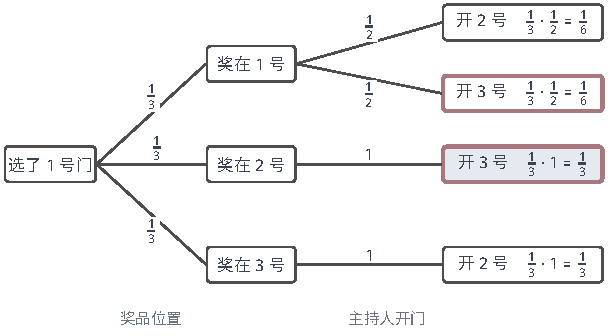
\includegraphics[width=103mm]{figures/07-probability/01-elementary-probability/tikz/cprob-three-doors-tree/figure.pdf}
  \caption{三扇门问题的树形图。第一层是奖品位置，第二层是主持人按规则开的门，分支上是条件概率，叶上是路径概率。红框的两片叶组成观察到的事件“打开3号门”，其中浅蓝的一片（奖在2号门后）占$\frac{1/3}{1/2}=\frac23$。}
  \label{fig:cprob-three-doors-tree}
\end{BookInlineFigure}

\paragraph{检测中的三个比例}
产品出厂前要经过一道自动检测。设某批产品中次品率为$2\%$；检测对次品报警的概率为$0.95$，对合格品误报的概率为$0.05$。一件产品报警了，它是次品的概率是多少？很多人会回答$0.95$，下面的计算说明这个答案错得很远。

令$D$为“次品”，$T$为“报警”。已知量是
\[
 \mathbb{P}(D)=0.02,\qquad \mathbb{P}(T\mid D)=0.95,\qquad \mathbb{P}(T\mid D^{\mathrm{c}})=0.05.
\]
$D$与$D^{\mathrm{c}}$构成划分。由全概率公式，报警的概率是
\[
 \mathbb{P}(T)=0.02\times0.95+0.98\times0.05=0.019+0.049=0.068.
\]
由Bayes公式，
\[
 \mathbb{P}(D\mid T)=\frac{0.019}{0.068}=\frac{19}{68}\approx0.279.
\]

图~\ref{fig:cprob-test-frequency-tree}用$10000$件产品把这些比例换成件数。$200$件次品中有$190$件报警，$9800$件合格品中有$490$件误报；报警的$680$件里只有$190$件是次品。误报率虽小，合格品的数量却大得多，误报的件数反而超过了真正的次品。

\begin{BookInlineFigure}
  \centering
  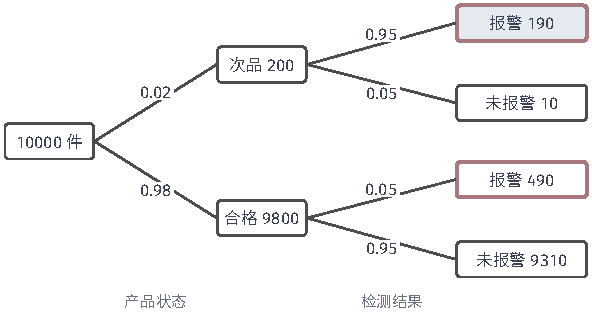
\includegraphics[width=100mm]{figures/07-probability/01-elementary-probability/tikz/cprob-test-frequency-tree/figure.pdf}
  \caption{用$10000$件产品表示检测的各个比例。分支上的数是条件概率，节点中是件数；红框是报警的两组，浅蓝的一组是报警且为次品，占报警件数的$190/680\approx0.279$。}
  \label{fig:cprob-test-frequency-tree}
\end{BookInlineFigure}

这个例子中三个数分别回答三个问题：先验比例$\mathbb{P}(D)=0.02$是检测前一件产品为次品的概率；条件检出概率$\mathbb{P}(T\mid D)=0.95$描述检测的性能，即在次品中报警的比例；后验比例$\mathbb{P}(D\mid T)\approx0.279$是在报警的产品中次品的比例。第二个与第三个的分子相同、分母不同，正是前面说的两个方向的条件概率。

\paragraph{信息的逐次更新}
报警的产品再送去复检一次。设复检用同样性能的设备，并假设：对给定状态的产品，复检是否报警不受第一次结果的影响，即
\[
 \mathbb{P}(T_2\mid D\cap T_1)=\mathbb{P}(T_2\mid D)=0.95,\qquad
 \mathbb{P}(T_2\mid D^{\mathrm{c}}\cap T_1)=\mathbb{P}(T_2\mid D^{\mathrm{c}})=0.05,
\]
其中$T_1,T_2$分别是两次报警。若两次报警之后才判定，次品的概率是多少？

已知$T_1$发生，就在$\mathbb{P}(\cdot\mid T_1)$下计算。由定理~\ref{thm:cprob-conditional-axioms}，它满足三条基本性质，所以全概率公式与Bayes公式对它同样成立。在它之下再以$D$为条件，得到的正是以$D\cap T_1$为条件：
\[
 \frac{\mathbb{P}(T_2\cap D\mid T_1)}{\mathbb{P}(D\mid T_1)}
 =\frac{\mathbb{P}(T_2\cap D\cap T_1)/\mathbb{P}(T_1)}{\mathbb{P}(D\cap T_1)/\mathbb{P}(T_1)}
 =\mathbb{P}(T_2\mid D\cap T_1).
\]
因此公式中的先验换成第一次报警后的后验$19/68$，条件检出概率换成上面假设的$\mathbb{P}(T_2\mid D\cap T_1)$与$\mathbb{P}(T_2\mid D^{\mathrm{c}}\cap T_1)$：
\[
 \mathbb{P}(D\mid T_1\cap T_2)
 =\frac{\frac{19}{68}\times0.95}{\frac{19}{68}\times0.95+\frac{49}{68}\times0.05}
 =\frac{18.05}{18.05+2.45}=\frac{361}{410}\approx0.880.
\]
一次观察后的后验成为下一次观察的先验，信息就这样逐次累积。

比值的写法更能看出每次更新做了什么。次品与合格品的概率之比，先验是$0.02:0.98=1:49$。由式~\eqref{eq:cprob-bayes}，两个后验的分母相同，比值只由分子决定：
\begin{equation}
 \frac{\mathbb{P}(D\mid T)}{\mathbb{P}(D^{\mathrm{c}}\mid T)}
 =\frac{\mathbb{P}(D)}{\mathbb{P}(D^{\mathrm{c}})}\cdot\frac{\mathbb{P}(T\mid D)}{\mathbb{P}(T\mid D^{\mathrm{c}})}.
 \label{eq:cprob-odds}
\end{equation}
右端第二个因子称为观察$T$的\term{似然比}（likelihood ratio），这里是$0.95/0.05=19$。每次报警把比值乘以$19$：一次后为$19:49$，即概率$19/68$；两次后为$361:49$，即概率$361/410$。

图~\ref{fig:cprob-posterior-prior}把后验画成先验次品率的函数。先验很小时，一次报警之后的后验仍然不大；同一个似然比作用在不同的先验上，结果可以相差很多。这再次说明，只知道检测的性能，不知道先验比例，无法回答“报警的产品有多大可能是次品”。

\begin{BookInlineFigure}
  \centering
  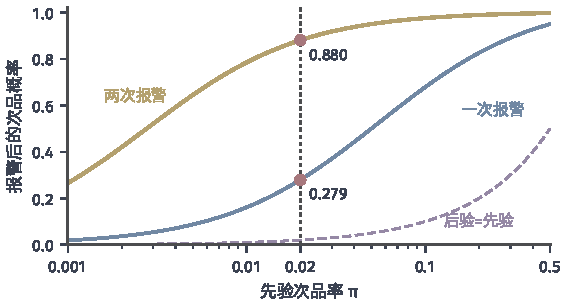
\includegraphics[width=96mm]{figures/07-probability/01-elementary-probability/matplotlib/cprob-posterior-prior/figure.pdf}
  \caption{报警后为次品的概率随先验次品率$\pi$的变化，横轴为对数坐标。检出概率$0.95$，误报概率$0.05$。蓝线是一次报警后的后验，黄线是两次报警后的后验（假设给定状态时两次检测互不影响），紫色虚线是后验等于先验的参考线；红点标出正文中$\pi=0.02$的两个值。}
  \label{fig:cprob-posterior-prior}
\end{BookInlineFigure}

两次更新所用的假设必须核对。如果某类次品的缺陷检测设备根本看不出来，第一次漏报的产品第二次也会漏报，两次结果就不再互不影响，乘以两次似然比会高估证据的强度。这个假设是对条件概率$\mathbb{P}(\cdot\mid D)$与$\mathbb{P}(\cdot\mid D^{\mathrm{c}})$的要求，下一节会看到它与“两次报警互不影响”并不是一回事。

\section{事件的独立性}
\label{sec:cprob-independence}

不放回摸球时，第一个球的颜色改变了第二个球的概率：$\mathbb{P}(H_2\mid H_1)=1/2$，而$\mathbb{P}(H_2)=3/5$。放回摸球时，第一个球摸出后又放了回去，盒中构成不变，无论第一个是什么颜色，第二个是黑球的概率都是$3/5$。在后一种情形下，知道第一个结果不提供关于第二个结果的任何信息，计算交事件的概率时可以把两个概率直接相乘。怎样把“不提供信息”准确地写出来？

\paragraph{定义}
放回摸球的有序记录有$25$个等可能结果，其中两个都是黑球的有$3\times3=9$个，所以
\[
 \mathbb{P}(H_2\mid H_1)=\frac{9/25}{15/25}=\frac35=\mathbb{P}(H_2).
\]
条件概率等于原来的概率，就是“已知$H_1$不改变$H_2$的可能性”。把等式$\mathbb{P}(H_2\mid H_1)=\mathbb{P}(H_2)$乘以$\mathbb{P}(H_1)$，得到一个对两个事件对称的乘积形式，并且在条件事件概率为零时也有意义。

\begin{definition}[两个事件的独立]
\label{def:cprob-independent}
若事件$A,B$满足
\begin{equation}
 \mathbb{P}(A\cap B)=\mathbb{P}(A)\,\mathbb{P}(B),
 \label{eq:cprob-independent}
\end{equation}
就称$A$与$B$\term{独立}（independent）。
\end{definition}

当$\mathbb{P}(B)>0$时，由定义~\eqref{eq:cprob-conditional}，式~\eqref{eq:cprob-independent}等价于$\mathbb{P}(A\mid B)=\mathbb{P}(A)$；当$\mathbb{P}(A)>0$时，它也等价于$\mathbb{P}(B\mid A)=\mathbb{P}(B)$。所以独立是对称的：$B$不提供关于$A$的信息，$A$也不提供关于$B$的信息。

\paragraph{独立是数量关系}
独立性要按式~\eqref{eq:cprob-independent}核对，不能凭“看起来有没有关系”判断。从一副$52$张的牌中抽一张，令$A$为“抽到A”，$B$为“抽到红桃”。四张A中恰有一张红桃，所以
\[
 \mathbb{P}(A\cap B)=\frac{1}{52},\qquad
 \mathbb{P}(A)\,\mathbb{P}(B)=\frac{4}{52}\cdot\frac{13}{52}=\frac{1}{52}.
\]
二者独立。原因在于一副牌是$13$种点数与$4$种花色的全部搭配，每种点数在各花色中出现的比例都相同。

掷两枚骰子，令$A$为“第一枚是偶数”，$C$为“点数和为$7$”，$D$为“点数和为$8$”。点数和要用到第一枚的点数，似乎不会与$A$独立。在图~\ref{fig:cprob-independence-grid}(a)中数一数：$A$占$18$格，$C$的$6$格中有$3$格落在$A$里，所以
\[
 \mathbb{P}(A\cap C)=\frac{3}{36}=\frac12\cdot\frac16=\mathbb{P}(A)\,\mathbb{P}(C).
\]
$A$与$C$独立。原因是对第一枚的每个点数$i$，第二枚都恰有一个点数$7-i$使和为$7$，和为$7$的比例在每一列中都是$1/6$。

\begin{BookInlineFigure}
  \centering
  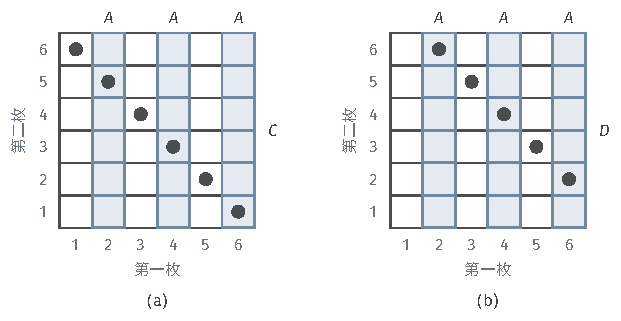
\includegraphics[width=105mm]{figures/07-probability/01-elementary-probability/tikz/cprob-independence-grid/figure.pdf}
  \caption{同一事件$A$（浅蓝三列，第一枚为偶数）与两个事件的关系。(a)圆点是$C$（点数和为$7$），在$A$内外各占所在列的$1/6$，$A$与$C$独立。(b)圆点是$D$（点数和为$8$），$A$内有$3$个、$A$外只有$2$个，$A$与$D$不独立。}
  \label{fig:cprob-independence-grid}
\end{BookInlineFigure}

$D$的情形不同。和为$8$的格子是$(2,6),(3,5),(4,4),(5,3),(6,2)$，其中第一枚为偶数的有$3$个，见图~\ref{fig:cprob-independence-grid}(b)。于是
\[
 \mathbb{P}(A\cap D)=\frac{3}{36},\qquad \mathbb{P}(A)\,\mathbb{P}(D)=\frac12\cdot\frac{5}{36}=\frac{2.5}{36}.
\]
两者不等，$A$与$D$不独立：第一枚为$1$时第二枚不可能凑出$8$，所以$D$在$A$之外的比例较低。对比$C$与$D$，事件之间在物理上是否“有关”不决定独立性，决定它的是交事件的比例。

\paragraph{独立与互斥}
互斥和独立都描述两个事件的关系，含义却几乎相反。互斥是集合之间的关系：$A\cap B=\varnothing$，两个事件不能同时发生，它与概率如何分配无关。独立是概率之间的关系：一个事件发生与否不改变另一个的概率，它取决于$\mathbb{P}$。

设$\mathbb{P}(A)>0$，$\mathbb{P}(B)>0$，且$A$与$B$互斥，则
\[
 \mathbb{P}(A\cap B)=0<\mathbb{P}(A)\,\mathbb{P}(B),
\]
二者不独立。这很合理：知道$B$发生，就确知$A$没有发生，$B$提供了关于$A$的完全信息。只有当其中一个事件的概率为零时，互斥的两个事件才独立。

\paragraph{补事件保持独立}
若$B$发生不提供关于$A$的信息，那么$B$不发生也不应提供信息。下面先对两个事件证实这一点，相互独立的多个事件在下一段定义之后再作推广。

\begin{theorem}[独立与补事件]
\label{thm:cprob-independent-complement}
若$A$与$B$独立，则$A$与$B^{\mathrm{c}}$独立，$A^{\mathrm{c}}$与$B$独立，$A^{\mathrm{c}}$与$B^{\mathrm{c}}$也独立。
\end{theorem}

\begin{proof}
$A$是互斥的$A\cap B$与$A\cap B^{\mathrm{c}}$之并，由互斥可加性与独立性，
\[
 \mathbb{P}(A\cap B^{\mathrm{c}})=\mathbb{P}(A)-\mathbb{P}(A\cap B)=\mathbb{P}(A)\bigl(1-\mathbb{P}(B)\bigr)=\mathbb{P}(A)\,\mathbb{P}(B^{\mathrm{c}}).
\]
所以$A$与$B^{\mathrm{c}}$独立。交换$A,B$的角色得到第二个结论；对独立的$A^{\mathrm{c}}$与$B$再用一次第一个结论，得到第三个。
\end{proof}

\paragraph{多个事件的相互独立}
三个或更多事件时，“互不提供信息”的要求更强：不仅任意两个之间不提供信息，任意几个事件的发生情况也不应改变其余事件的概率。这需要对所有子组都验证乘积关系。

\begin{definition}[相互独立]
\label{def:cprob-mutually-independent}
称事件$A_1,\ldots,A_n$\term{相互独立}（mutually independent），若对任意$2\leq k\leq n$和任意下标$1\leq i_1<\cdots<i_k\leq n$，都有
\begin{equation}
 \mathbb{P}(A_{i_1}\cap\cdots\cap A_{i_k})=\mathbb{P}(A_{i_1})\cdots\mathbb{P}(A_{i_k}).
 \label{eq:cprob-mutually-independent}
\end{equation}
若只要求$k=2$的情形，即任意两个事件独立，就称它们\term{两两独立}（pairwise independent）。
\end{definition}

两两独立不能推出相互独立。抛两枚均匀硬币，四个有序结果等可能。令$A$为“第一枚正面”，$B$为“第二枚正面”，$C$为“两枚结果相同”。每个事件的概率都是$1/2$；由图~\ref{fig:cprob-two-coins-pairwise}，任意两个事件恰好共有一个结果，所以每对的交的概率都是$1/4=(1/2)^2$，三对都独立。

\begin{BookInlineFigure}
  \centering
  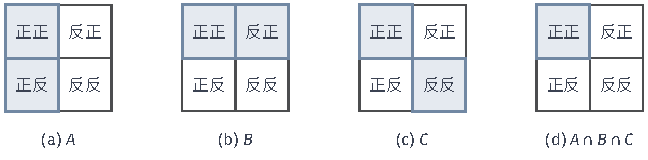
\includegraphics[width=110mm]{figures/07-probability/01-elementary-probability/tikz/cprob-two-coins-pairwise/figure.pdf}
  \caption{抛两枚硬币的四个等可能结果，“正反”表示第一枚正面、第二枚反面。浅蓝格子依次是(a)$A$：第一枚正面；(b)$B$：第二枚正面；(c)$C$：两枚相同；(d)$A\cap B\cap C$。任意两个事件的交都只有“正正”一格，三者之交也只有这一格。}
  \label{fig:cprob-two-coins-pairwise}
\end{BookInlineFigure}

但三个事件同时发生就是“正正”，于是
\[
 \mathbb{P}(A\cap B\cap C)=\frac14\neq\frac18=\mathbb{P}(A)\,\mathbb{P}(B)\,\mathbb{P}(C).
\]
三者不相互独立。原因很清楚：知道$A$与$B$都发生，就完全知道了$C$；单独知道其中任何一个，却对另一个毫无帮助。

反过来，只验证三者之交的乘积关系也不够。掷两枚骰子，令$E_1$为“第一枚是$1,2,3$之一”，$E_2$为“第一枚是$3,4,5$之一”，$E_3$为“点数和为$9$”。$E_1\cap E_2\cap E_3$只有结果$(3,6)$，于是
\[
 \mathbb{P}(E_1\cap E_2\cap E_3)=\frac{1}{36}=\frac12\cdot\frac12\cdot\frac19.
\]
然而$E_1\cap E_2$是“第一枚是$3$”，概率$1/6\neq1/4$，这两个事件不独立。定义~\ref{def:cprob-mutually-independent}要求所有子组的乘积关系，任何一层都不能省略。

\paragraph{多个事件的补}
定理~\ref{thm:cprob-independent-complement}可以推广到相互独立的多个事件：把其中任意几个换成补事件，所得的事件仍相互独立。只需说明换掉一个即可，换多个时逐个替换。设$A_1,\ldots,A_n$相互独立，把$A_1$换成$A_1^{\mathrm{c}}$。对含下标$1$的子组，记其余事件之交为$F$。由于$A_1,\ldots,A_n$的乘积关系对每个子组成立，$\mathbb{P}(F)$等于其余各事件概率之积，并且
\[
 \mathbb{P}(A_1\cap F)=\mathbb{P}(A_1)\,\mathbb{P}(F).
\]
重复定理~\ref{thm:cprob-independent-complement}的证明，得到
\[
 \mathbb{P}(A_1^{\mathrm{c}}\cap F)=\mathbb{P}(F)-\mathbb{P}(A_1\cap F)=\mathbb{P}(A_1^{\mathrm{c}})\,\mathbb{P}(F).
\]
不含下标$1$的子组不受影响，所以式~\eqref{eq:cprob-mutually-independent}对新的一组事件仍成立。

\paragraph{重复试验中的独立性从哪里来}
“两次投掷互不影响”这句话，在模型中究竟对应什么？以两枚骰子为例，样本空间是乘积$\Omega=\Omega_1\times\Omega_2$，$\Omega_1=\Omega_2=\{1,\ldots,6\}$，第~\ref{sec:cprob-equally-likely}节假设这$36$个有序对同样可能。只与第一枚有关的事件形如$A_1\times\Omega_2$，只与第二枚有关的事件形如$\Omega_1\times A_2$，它们的交是矩形$A_1\times A_2$，如图~\ref{fig:cprob-product-space}所示。

\begin{BookInlineFigure}
  \centering
  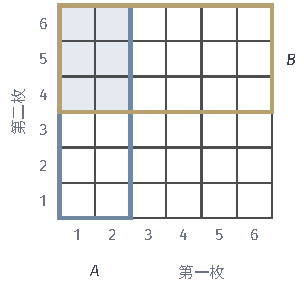
\includegraphics[width=53mm]{figures/07-probability/01-elementary-probability/tikz/cprob-product-space/figure.pdf}
  \caption{乘积样本空间中的独立性。蓝框是$A$：第一枚为$1$或$2$；黄框是$B$：第二枚为$4,5,6$之一。交$A\cap B$是$2\times3$的浅蓝矩形，其格数等于两边格数之积。}
  \label{fig:cprob-product-space}
\end{BookInlineFigure}

\begin{theorem}[乘积样本空间上的独立性]
\label{thm:cprob-product-independence}
设$\Omega=\Omega_1\times\cdots\times\Omega_n$，各$\Omega_k$有限且非空，$\Omega$上的全部结果同样可能。对每个$k$取$A_k\subseteq\Omega_k$，令
\begin{equation}
 E_k=\{(\omega_1,\ldots,\omega_n)\in\Omega:\ \omega_k\in A_k\}
 \label{eq:cprob-coordinate-event}
\end{equation}
为只与第$k$个分量有关的事件。则$E_1,\ldots,E_n$相互独立，并且
\begin{equation}
 \mathbb{P}(E_k)=\frac{\lvert A_k\rvert}{\lvert\Omega_k\rvert}.
 \label{eq:cprob-product-marginal}
\end{equation}
\end{theorem}

\begin{proof}
任取下标集合$S\subseteq\{1,\ldots,n\}$。按式~\eqref{eq:cprob-coordinate-event}，$\bigcap_{k\in S}E_k$由第$k$个分量在$A_k$中（$k\in S$）、其余分量任意的结果组成，它是乘积集合，各分量的取值范围分别是$A_k$（$k\in S$）或$\Omega_k$（$k\notin S$）。由乘法规则计数，
\[
 \Bigl\lvert\bigcap_{k\in S}E_k\Bigr\rvert=\prod_{k\in S}\lvert A_k\rvert\prod_{k\notin S}\lvert\Omega_k\rvert.
\]
$\Omega$本身也是乘积集合，$\lvert\Omega\rvert$等于各$\lvert\Omega_k\rvert$之积。两式相除，得到
\[
 \mathbb{P}\Bigl(\bigcap_{k\in S}E_k\Bigr)=\prod_{k\in S}\frac{\lvert A_k\rvert}{\lvert\Omega_k\rvert}.
\]
取$S=\{k\}$即得式~\eqref{eq:cprob-product-marginal}；把它代回上式，对每个至少含两个下标的$S$都得到式~\eqref{eq:cprob-mutually-independent}。
\end{proof}

定理说明，重复试验中的独立性是乘积样本空间上等可能假设的推论。这个假设比“每次试验各自等可能”更多：它还要求各次结果的每种搭配同样可能，这正是“互不影响”在模型中的含义。放回摸球的$25$个有序对是$\{1,\ldots,5\}\times\{1,\ldots,5\}$的全部，满足定理的条件，所以$H_1$与$H_2$独立。

不放回摸球的样本空间去掉了对角线，不再是乘积集合，定理不适用；实际计算也表明$\mathbb{P}(H_1\cap H_2)=3/10$，而$\mathbb{P}(H_1)\,\mathbb{P}(H_2)=9/25$，二者不独立。每一次单独看，第二个球在五个球中仍是等可能的，$\mathbb{P}(H_2)=3/5$；不独立来自两次之间的搭配受到限制。

\paragraph{至少成功一次}
独立性使“$n$次重复中至少成功一次”的计算变得简单。设每次试验中某事件发生的概率为$p$，各次的事件相互独立。由上面关于补事件的推广，各次“不发生”的事件也相互独立，所以$n$次都不发生的概率是$(1-p)^{n}$，于是
\begin{equation}
 \mathbb{P}(\text{至少发生一次})=1-(1-p)^{n}.
 \label{eq:cprob-at-least-once}
\end{equation}

一个经典的比较是：掷一枚骰子$4$次至少出现一个六点，与掷两枚骰子$24$次至少出现一次双六，哪个更可能？前者$p=1/6$，后者$p=1/36$，由式~\eqref{eq:cprob-at-least-once}，
\[
 1-\Bigl(\frac56\Bigr)^{4}\approx0.5177,\qquad
 1-\Bigl(\frac{35}{36}\Bigr)^{24}\approx0.4914.
\]
虽然$4/6=24/36$，两者却一个略大于一半、一个略小于一半。图~\ref{fig:cprob-repeated-trials}画出两条曲线：概率不是随次数线性增长，而是以$1-(1-p)^{n}$的形式逐渐接近$1$，“机会乘以次数”只在$np$很小时近似成立。

\begin{BookInlineFigure}
  \centering
  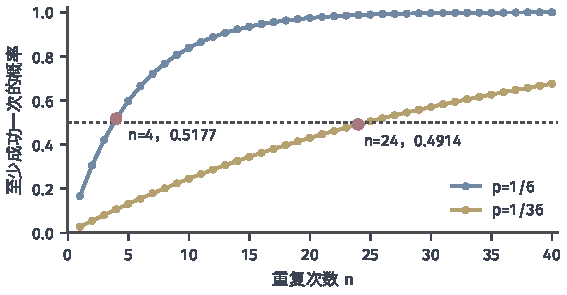
\includegraphics[width=96mm]{figures/07-probability/01-elementary-probability/matplotlib/cprob-repeated-trials/figure.pdf}
  \caption{$n$次独立重复中至少成功一次的概率$1-(1-p)^{n}$。蓝线$p=1/6$（一枚骰子出六点），黄线$p=1/36$（两枚骰子出双六），黑色点线是$1/2$；红点标出$n=4$与$n=24$两个值。}
  \label{fig:cprob-repeated-trials}
\end{BookInlineFigure}

同样的论证给出：$n$次中指定的$k$次成功、其余失败的概率是$p^{k}(1-p)^{n-k}$。在古典模型中$p$只能是有理数，例如$1/6$；成功次数的完整分布以及一般的$p$在第~\ref{chap:common-distributions}章讨论。

\paragraph{条件之下的独立}
回到第~\ref{sec:cprob-total-bayes}节的复检。那里假设的是：对次品，两次检测是否报警互不影响；对合格品也是如此。用本节的语言，就是$T_1$与$T_2$在条件概率$\mathbb{P}(\cdot\mid D)$下独立，在$\mathbb{P}(\cdot\mid D^{\mathrm{c}})$下也独立：
\[
 \mathbb{P}(T_1\cap T_2\mid D)=0.95^{2},\qquad
 \mathbb{P}(T_1\cap T_2\mid D^{\mathrm{c}})=0.05^{2}.
\]

不按状态区分时，$T_1$与$T_2$并不独立。由全概率公式，
\[
 \mathbb{P}(T_1\cap T_2)=0.02\times0.9025+0.98\times0.0025=0.0205,
\]
而两次报警各自的概率都是$0.068$，乘积为
\[
 \mathbb{P}(T_1)\,\mathbb{P}(T_2)=0.068^{2}\approx0.0046.
\]第一次报警提高了产品是次品的可能性，从而提高了第二次报警的可能性，两次报警通过产品的状态联系在一起。条件之下的独立与不加条件的独立是两回事，一般理论在第~\ref{chap:conditional-distributions}章建立。

\section{模型的适用范围}
\label{sec:cprob-scope}

古典模型的全部计算都建立在一个前提上：样本空间有限，每个样本点同样可能。前面几节一再看到，同一个试验换一种记录方式，这个前提就可能不再成立。本节把失效的情形归为三类：记录合并了不等量的基本结果、结果有无穷多个、结果取连续的位置。对每一类，我们说明计数比为什么失效，以及后面的章节用什么代替它。

\paragraph{合并后的结果}
掷两枚骰子，如果只记录出现了哪两个点数而不分先后，结果就是可重复的无序对，例如$\{1,1\}$、$\{1,2\}$、$\{3,5\}$。由表~\ref{tab:cprob-sampling}最后一行，这样的结果共有$\binom{6+2-1}{2}=21$个。它们是否同样可能？

图~\ref{fig:cprob-merged-classes}显示了每个无序结果合并了哪些有序结果。对角线上的$\{i,i\}$只对应一个有序对$(i,i)$，概率是$1/36$；其余的$\{i,j\}$（$i\neq j$）对应关于对角线对称的两个格子$(i,j)$与$(j,i)$，概率是$2/36$。$6$个一类、$15$个另一类，验证总和：
\[
 6\times\frac{1}{36}+15\times\frac{2}{36}=\frac{36}{36}=1.
\]

\begin{BookInlineFigure}
  \centering
  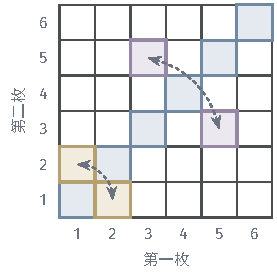
\includegraphics[width=47mm]{figures/07-probability/01-elementary-probability/tikz/cprob-merged-classes/figure.pdf}
  \caption{不记次序时两枚骰子的结果。浅蓝的对角线格子各自构成一个无序结果$\{i,i\}$；其余无序结果各由关于对角线对称的两个格子组成，黄色一对是$\{1,2\}$，紫色一对是$\{3,5\}$，虚线连接同一结果的两个格子。}
  \label{fig:cprob-merged-classes}
\end{BookInlineFigure}

若直接在$21$个无序结果上数，“两枚点数相同”占$6$个，会得到$6/21=2/7$；正确的答案是$6/36=1/6$。错误不在于用无序记录，而在于把合并了不同数量基本结果的类别当成了等可能的点。

一般地，若一个结果$r$是若干个等可能基本结果合并而成的，它的概率等于所合并的基本结果的概率之和。合并的个数不同，各结果的概率就不同。这时仍可以计算，但要给每个结果单独记一个概率$p(r)\geq0$，所有$p(r)$之和为$1$，事件的概率是它所含结果的$p(r)$之和。摸球的颜色记录、点数和、无序的点数对都属于这种情形，第~\ref{sec:cprob-equally-likely}节的三条基本性质对这样的分配仍然成立。

有些试验根本没有一个等可能的细化。一枚重心偏移的骰子，六个面朝上的机会本来就不同，无论怎样细分记录都找不到对称性。古典模型对它无能为力，只能直接给六个面各指定一个概率。给有限或可数个结果逐一指定概率的方式称为概率表，它在第~\ref{chap:random-variables}章与随机变量一起建立。

\paragraph{无穷多个结果}
抛一枚均匀硬币，直到第一次出现正面为止，记下所抛的次数。结果可以是$1,2,3,\ldots$中的任何一个，样本空间$\Omega=\{1,2,3,\ldots\}$有无穷多个点。

这些结果不可能同样可能。若每个结果的概率都是同一个数$c$，那么$c>0$时，任意取$N>1/c$个结果，它们的概率之和就超过$1$；$c=0$时，所有结果的概率都是零，总和无法是$1$。计数比$\lvert A\rvert/\lvert\Omega\rvert$在这里更没有意义，分母是无穷。

各结果的概率可以从有限的古典模型中算出。“第一次正面出现在第$k$次”只与前$k$次有关，它要求前$k-1$次都是反面、第$k$次是正面。前$k$次的$2^{k}$个有序结果等可能，满足要求的只有一个，所以
\begin{equation}
 \mathbb{P}(\text{第一次正面出现在第}k\text{次})=\frac{1}{2^{k}},\qquad k=1,2,\ldots.
 \label{eq:cprob-first-head}
\end{equation}

图~\ref{fig:cprob-first-head}(a)画出这些概率，它们随$k$成倍减小。前$k$项之和是$1-2^{-k}$，见图~\ref{fig:cprob-first-head}(b)，它随$k$增大而趋于$1$，但任何有限项之和都小于$1$。要让总概率等于$1$，必须把无穷多个结果的概率加起来，这要求可加性从有限个事件推广到可数个事件。

\begin{BookInlineFigure}
  \centering
  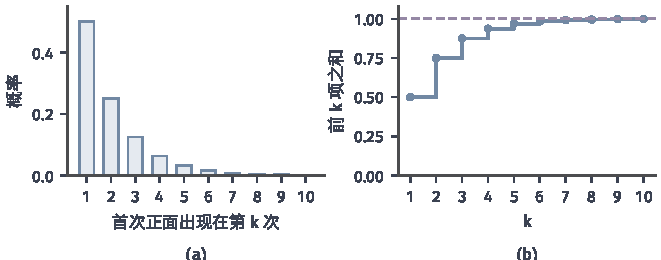
\includegraphics[width=112mm]{figures/07-probability/01-elementary-probability/matplotlib/cprob-first-head/figure.pdf}
  \caption{抛硬币直到第一次正面。(a)第一次正面出现在第$k$次的概率$2^{-k}$；(b)前$k$项之和$1-2^{-k}$，紫色虚线是总和$1$，有限项之和都达不到它。}
  \label{fig:cprob-first-head}
\end{BookInlineFigure}

\paragraph{连续的位置}
在长为$1$的木棍上随机选一个点，点的位置可以是$[0,1]$中的任何实数。所谓“随机”，自然的意思是长度相同的两段被选中的机会相同。问点落在$(0.2,0.5]$中的概率是多少？

计数比在这里给不出答案：$(0.2,0.5]$与$[0,1]$都有无穷多个点，比值是“无穷比无穷”。可以先用有限模型逼近：在$(0,1]$上取$n$个等距位置$k/n$，$k=1,\ldots,n$，让它们等可能。这是一个古典模型，事件“落在$(0.2,0.5]$中”的概率是其中位置的个数除以$n$。

图~\ref{fig:cprob-grid-uniform}(a)显示，随着$n$增大，这个计数比趋于区间的长度$0.3$。例如$n=10$时恰有$3$个位置，比值是$0.3$；$n=7$时有$k=2,3$两个位置，比值是$2/7\approx0.286$。另一方面，图~\ref{fig:cprob-grid-uniform}(b)中单个位置的概率$1/n$趋于$0$。

\begin{BookInlineFigure}
  \centering
  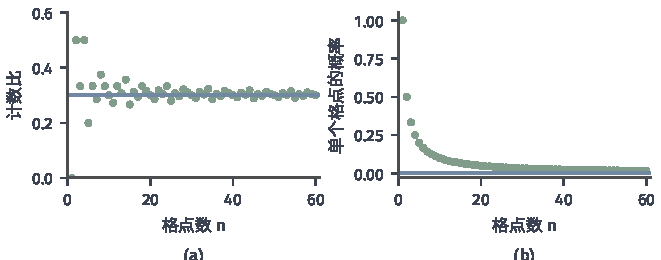
\includegraphics[width=112mm]{figures/07-probability/01-elementary-probability/matplotlib/cprob-grid-uniform/figure.pdf}
  \caption{用$n$个等距位置$k/n$逼近木棍上的随机点。(a)绿点是事件“落在$(0.2,0.5]$中”的计数比，蓝线是区间长度$0.3$；(b)绿点是单个位置的概率$1/n$，趋于蓝线$0$。}
  \label{fig:cprob-grid-uniform}
\end{BookInlineFigure}

这两个极限提示了连续情形的做法：区间的概率由长度给出，不由点数给出；每个单点的概率都是$0$，但每个点都可能被选中。概率为零不等于不可能，这在有限的古典模型中不会发生，那里$\mathbb{P}(A)=0$当且仅当$A=\varnothing$。长度的作用在一般情形中由密度承担，单位长度上的概率可以随位置变化，第~\ref{chap:random-variables}章用积分计算这类概率。

\paragraph{三类情形的统一}
表~\ref{tab:cprob-models}把本节的几种情形放在一起。它们分配概率的方式不同，但都应当满足非负、总量为$1$、互斥事件的概率相加这几条要求；可数个结果和连续位置还要求可加性对可数个互斥事件成立。

\begin{BookInlineTable}
  \centering
  \caption{几类概率模型分配概率的方式}
  \label{tab:cprob-models}
  \begin{tabular}{lll}
    \toprule
    样本空间 & 例子 & 事件的概率 \\
    \midrule
    有限，等可能 & 均匀骰子、摸球 & 计数比$\lvert A\rvert/\lvert\Omega\rvert$ \\
    有限，不等可能 & 点数和、偏心骰子 & 所含结果的概率之和 \\
    可数无穷 & 首次正面的次数 & 所含结果的概率之和（级数） \\
    连续位置 & 木棍上的点 & 长度，一般为密度的积分 \\
    \bottomrule
  \end{tabular}
\end{BookInlineTable}

把这些情形纳入同一个框架，需要回答哪些集合可以作为事件、概率怎样对可数个事件相加，以及长度这样的量能定义在哪些集合上。这些问题在第~\ref{chap:probability-spaces}章用概率测度统一回答。在此之前，第~\ref{chap:random-variables}章先用概率表和密度直接处理有限、可数与连续的情形。

\section{本章小结}
\label{sec:cprob-summary}

本章用一个盒子贯穿始终：$3$个黑球、$2$个白球，摸出两个。把这次抽样从头算一遍，就能把本章的概念串起来，并看清各步依赖的假设。表~\ref{tab:cprob-summary}按顺序列出各步。

\begin{BookInlineTable}
  \centering
  \caption{摸球问题中各步的计算与所用假设}
  \label{tab:cprob-summary}
  \begin{tabular}{lll}
    \toprule
    步骤 & 计算 & 所用假设 \\
    \midrule
    样本空间 & 有序对共$20$个 & 记录先后，细到能表达事件 \\
    等可能 & 每个有序对概率$1/20$ & 搅匀后每个球机会相同 \\
    计数 & $\mathbb{P}(H_1\cap H_2)=6/20$ & 分子分母同一口径 \\
    条件概率 & $\mathbb{P}(H_2\mid H_1)=2/4$ & $\mathbb{P}(H_1)>0$ \\
    乘法规则 & $\tfrac35\cdot\tfrac24=\tfrac{3}{10}$ & 条件随已摸结果改变 \\
    全概率 & $\mathbb{P}(H_2)=\tfrac{6}{20}+\tfrac{6}{20}=\tfrac35$ & $H_1,H_1^{\mathrm{c}}$构成划分 \\
    Bayes & $\mathbb{P}(H_1\mid H_2)=1/2$ & $\mathbb{P}(H_2)>0$ \\
    独立性 & 不放回不独立，放回独立 & 放回时乘积空间等可能 \\
    \bottomrule
  \end{tabular}
\end{BookInlineTable}

\paragraph{样本空间与计数}
概率首先要有一个样本空间：它列出一次试验的全部可能结果，事件是其中的子集，一次试验只产生一个结果，却可以让许多事件同时发生。样本空间由记录方式决定，它必须细到能表达所关心的事件。在有限且等可能的前提下，事件的概率是计数比$\lvert A\rvert/\lvert\Omega\rvert$，它满足非负、归一和互斥可加三条性质，补事件公式、加法公式与联合界都从这三条推出。

等可能是对试验的假设，依据是物理的对称性，不是样本点名称的对称。点数和、颜色记录、无序的可重复组合都合并了不同数量的基本结果，不能直接数类别。计数时分子和分母必须在同一个样本空间中数；放回与不放回改变的是样本空间本身。相对频率可以检验等可能假设是否与试验相符，但本章不用它定义概率。

\paragraph{条件与独立}
条件概率把样本范围缩小到已知发生的事件$B$，在其中按原比例重新归一，要求$\mathbb{P}(B)>0$。由它得到乘法规则，可以沿试验过程逐步计算；按划分分组得到全概率公式，再反推来源得到Bayes公式。先验、条件检出概率和后验分别回答不同的问题，$\mathbb{P}(A\mid B)$与$\mathbb{P}(B\mid A)$不能互换。逐次更新时，前一次的后验成为下一次的先验，但每次乘以似然比都要求给定状态时各次观察互不影响。

独立是交事件概率等于乘积这一数量关系，它与互斥不同，也不由“物理上是否有关”决定。多个事件的相互独立要求所有子组的乘积关系，两两独立或只验证全体之交都不够。重复试验中的独立性来自乘积样本空间上的等可能假设，不放回抽样不满足这一假设。条件之下的独立与不加条件的独立是两回事。

\paragraph{边界与下一步}
古典模型严格而具体，但只适用于有限且等可能的结果。结果不等可能时要逐个指定概率；结果有可数无穷多个时，可加性必须推广到可数个事件；结果取连续位置时，单点的概率为零，区间的概率要由长度或密度给出。下一章把试验的结果记录成数值，引入随机变量，用概率表、分布函数和密度描述它取各种值的概率，这三类情形都在那里得到具体的处理。


\chapter{随机变量的分布}
\label{chap:random-variables}

掷两枚骰子，赌局只看点数之和；从一批产品里抽两件检验，质检员只记次品有几件；在窗口前排队，顾客只在意等了几分钟。试验的结果本身可能很复杂，我们真正关心的却往往是由结果算出的一个数。这个数事先不知道，但它可能取哪些值、落在各个范围里的概率有多大，是可以说清楚的。

把这些问题写下来，就是本章要处理的几件事。点数之和等于$7$的概率是多少？次品不超过一件的概率是多少？等待时间落在$1$到$2$分钟之间的概率是多少？反过来，给定$90\%$这样的比例，多长的等待才能覆盖九成顾客？还有一个更基本的问题：用什么样的一张表或一个函数，才能一次记下所有这些答案？

第~\ref{chap:classical-probability}章在有限个等可能结果上计算事件的概率。本章先把“由结果算出的数”写成样本空间上的函数，即随机变量，并把注意力从具体结果转到它的取值规律，即分布。接着用分布函数统一记录实轴上的累计概率，再分别用概率质量和密度给出离散取值与连续取值时更直接的表示。分位数从反方向读分布函数，回答“给定概率，阈值在哪里”。最后检查这些表示各自的适用范围：有些分布既不能写成一张概率表，也没有密度，只有分布函数始终可用。

全章反复使用几个能手算的模型：骰子、不放回抽检、首次掷出六点所需的次数，以及以分钟计的等待时间。读者只需要第~\ref{chap:classical-probability}章的计数与条件概率，以及卷一的级数与积分。

\section{随机变量}
\label{sec:rvd-random-variables}

掷一枚骰子，样本空间是$\Omega=\{1,2,3,4,5,6\}$。如果关心点数，就把结果$\omega$记成数$\omega$；如果只关心奇偶，就把偶数结果记成$1$、奇数结果记成$0$。两种记录面对的是同一次试验，区别只在于“结果怎样变成数”。这种记录规则怎样精确表述，它取各个值的概率又怎样从结果的概率得到？

\paragraph{结果到数值的映射}
图~\ref{fig:rvd-die-maps}画出了两种记录。中间一行是六个结果，向上的箭头把每个结果送到它的点数，向下的箭头把三个偶数结果送到$1$、三个奇数结果送到$0$。两种记录都是从$\Omega$到实数的函数，只是第二个函数把不同的结果合并到了同一个值。

\begin{BookInlineFigure}
  \centering
  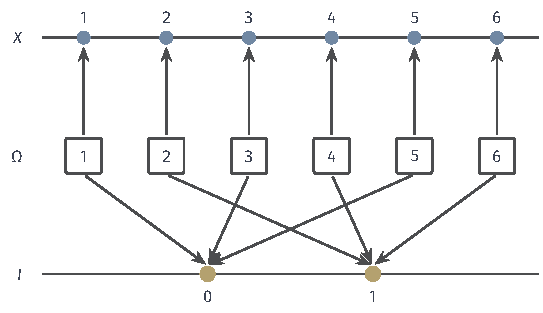
\includegraphics[width=92mm]{figures/07-probability/01-elementary-probability/tikz/rvd-die-maps/figure.pdf}
  \caption{同一次掷骰上的两个随机变量。中间一行是样本空间$\Omega$的六个结果。向上的箭头是点数$X$，六个结果送到六个不同的值（蓝点）；向下的箭头是奇偶记录$I$，三个奇数结果都送到$0$，三个偶数结果都送到$1$（黄点）。}
  \label{fig:rvd-die-maps}
\end{BookInlineFigure}

把这种规则一般地写出来，就得到随机变量。它的定义只用到样本空间和函数，概率在下一步才进入。

\begin{definition}[随机变量]
\label{def:rvd-random-variable}
设$\Omega$是一个试验的样本空间。函数$X:\Omega\to\mathbb{R}$称为\term{随机变量}（random variable）。对实数集的子集$B$，记
\begin{equation}
  \{X\in B\}=\{\omega\in\Omega:X(\omega)\in B\},
  \label{eq:rvd-preimage}
\end{equation}
它是由满足$X(\omega)\in B$的结果组成的事件，其概率记作$\mathbb{P}(X\in B)$。
\end{definition}

常用的事件有简写：$\{X\leq x\}$表示$B=(-\infty,x]$，$\{X=x\}$表示$B=\{x\}$，$\{a<X\leq b\}$表示$B=(a,b]$。在骰子的例子里，点数记录是$X(\omega)=\omega$，奇偶记录是
\[
  I(\omega)=\begin{cases}1,&\omega\in\{2,4,6\},\\0,&\omega\in\{1,3,5\}.\end{cases}
\]
于是$\{I=1\}=\{2,4,6\}$，$\{X\leq 2\}=\{1,2\}$，它们都是$\Omega$的子集，也就是第~\ref{chap:classical-probability}章意义下的事件。

一般地，对事件$A$，在$A$上取$1$、在$A$外取$0$的函数记作$\mathbf{1}_{A}$，称为$A$的\term{指示函数}（indicator function）。奇偶记录就是$I=\mathbf{1}_{\{2,4,6\}}$。指示函数把事件和随机变量联系起来：$\{\mathbf{1}_{A}=1\}=A$，所以$\mathbb{P}(\mathbf{1}_{A}=1)=\mathbb{P}(A)$。事件可以看成只取$0$和$1$的随机变量。

\paragraph{随机变量、实现值与事件}
“随机变量”这个名字容易误导：$X$本身是一个完全确定的函数，随机的是哪个结果$\omega$出现。试验做完，结果$\omega$确定，$X$就取一个具体的数$x=X(\omega)$，称为$X$的一个\term{实现值}（realization）。我们用大写字母表示随机变量，小写字母表示它的取值。

三种对象要分清。$X$是规则，在试验之前就已给定；$\{X\leq 2\}$是事件，是一个由结果组成的集合，事先可以问它的概率；“这次掷出$x=5$”是一次实现，事后才知道。说“$\mathbb{P}(X\leq 2)=1/3$”是在谈事件，说“$x=5>2$，所以事件$\{X\leq2\}$这次没有发生”是在用实现值检验事件。

\paragraph{由结果的概率得到取值的概率}
骰子公平时，每个结果的概率是$1/6$。要算$I$取$1$的概率，就把被送到$1$的结果的概率加起来：
\[
  \mathbb{P}(I=1)=\mathbb{P}(\{2,4,6\})=\tfrac16+\tfrac16+\tfrac16=\tfrac12 .
\]
可以把$\mathbb{P}$想成单位质量在六个结果上的分配，每个结果分到$1/6$。随机变量沿箭头把每个结果的质量搬到它的取值上，同一个取值收到的质量相加。$X$把六份质量分别搬到$1,\dots,6$，$I$把三份搬到$0$、三份搬到$1$。

同一个函数配上不同的概率，搬运的结果就不同。设骰子被做了手脚，$\mathbb{P}(\{6\})=1/2$，其余五面各为$1/10$。函数$I$没有变，但
\[
  \mathbb{P}(I=1)=0.1+0.1+0.5=0.7 .
\]
所以随机变量取值的概率规律由两样东西共同决定：结果到数值的规则$X$，以及结果上的概率$\mathbb{P}$。

\paragraph{无限多个结果}
等待时间可以是任何非负实数，样本空间$\Omega=[0,\infty)$有无穷多个结果，第~\ref{chap:classical-probability}章的计数比不再适用。本部分对这类试验直接规定区间事件的概率：例如规定等待超过$t$分钟的概率，再由加减得到其他区间的概率。具体的规定方式由下一节的分布函数和第~\ref{sec:rvd-mass-density}节的密度给出。

这样做时只对区间及其有限并谈概率，对取有限或可数个值的变量则对取值的任意子集谈概率。一般样本空间上哪些集合可以赋予概率、怎样保证各种规定彼此相容，在第~\ref{chap:probability-spaces}章统一处理。本部分用到的事件都是上面这些具体的集合，不会遇到困难。

\paragraph{同一次试验的不同记录}
同一次试验可以同时定义许多随机变量。掷两枚骰子，样本空间是$36$个等可能的有序对$\omega=(i,j)$。记点数之和为$S(\omega)=i+j$，较大的点数为$M(\omega)=\max\{i,j\}$。两者都是$\Omega$上的函数，记录的是同一次投掷的不同侧面。

事件$\{S=7\}$由反对角线上的六个结果组成，所以$\mathbb{P}(S=7)=6/36$。事件$\{M=4\}$由“较大者恰为$4$”的结果组成：$(4,1),\dots,(4,4)$与$(1,4),(2,4),(3,4)$，共$7$个，所以$\mathbb{P}(M=4)=7/36$。图~\ref{fig:rvd-two-dice}(a)用圆点和方框标出了这两个事件，$(3,4)$和$(4,3)$同时属于两者。

\begin{BookInlineFigure}
  \centering
  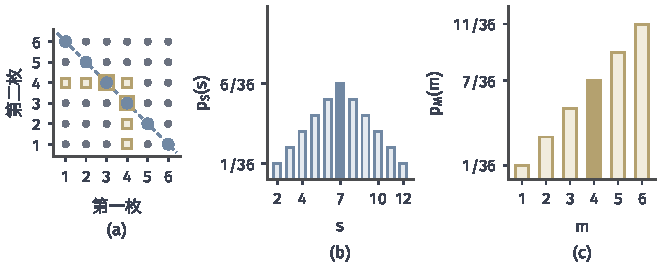
\includegraphics[width=112mm]{figures/07-probability/01-elementary-probability/matplotlib/rvd-two-dice/figure.pdf}
  \caption{两枚公平骰子上的两个随机变量。(a)$36$个等可能结果，蓝色圆点（沿虚线）是事件$\{S=7\}$，黄色方框是事件$\{M=4\}$，两个结果同时属于二者。(b)点数之和$S$取各值的概率，深色柱是$s=7$。(c)较大点数$M$取各值的概率，深色柱是$m=4$。}
  \label{fig:rvd-two-dice}
\end{BookInlineFigure}

对每个取值都这样计数，就得到图~\ref{fig:rvd-two-dice}(b)(c)。和为$s$的结果沿一条反对角线排列，条数先增后减，于是
\begin{equation}
  \mathbb{P}(S=s)=\frac{6-\lvert s-7\rvert}{36},\qquad s=2,3,\dots,12 .
  \label{eq:rvd-dice-sum}
\end{equation}
较大点数先用累计事件计数更方便：$\{M\leq m\}$要求两枚骰子都不超过$m$，有$m^{2}$个结果。$\{M=m\}$是$\{M\leq m\}$去掉$\{M\leq m-1\}$，所以
\[
  \mathbb{P}(M=m)=\frac{m^{2}-(m-1)^{2}}{36}=\frac{2m-1}{36},\qquad m=1,\dots,6 .
\]
两张表的概率各自加起来都等于$1$。

两个记录来自同一次投掷，彼此并不无关。知道$M=1$，就只能是$(1,1)$，于是$S=2$。这种同时考察多个随机变量的问题由第~\ref{chap:random-vectors}章处理，本章每次只看一个随机变量。

\paragraph{分布}
算出$\mathbb{P}(S=s)$之后，回答“$S$落在某个范围的概率”就不再需要回到$36$个结果：例如$\mathbb{P}(S\geq 10)=(3+2+1)/36=1/6$。我们只关心一个随机变量本身时，需要的正是这种“取值落在哪里、概率多大”的规律。

\begin{definition}[分布]
\label{def:rvd-distribution}
随机变量$X$的\term{分布}（probability distribution）是对实数集的子集$B$给出概率的规则
\begin{equation}
  P_X(B)=\mathbb{P}(X\in B)=\mathbb{P}(\{\omega\in\Omega:X(\omega)\in B\}).
  \label{eq:rvd-distribution}
\end{equation}
本部分中$B$取区间及其有限并；$X$只取有限或可数个值时，$B$可取这些值组成的任意集合。
\end{definition}

按搬运质量的图景，$\mathbb{P}$是单位质量在样本空间上的分配，$P_X$是这些质量被$X$搬到实轴之后的分配。分布只记录质量最后停在哪里，不再记录它从哪个结果搬来。这既是分布的用处，也是它的局限：凡是只涉及$X$一个变量取值的概率问题，分布都能回答；凡是涉及“哪个结果产生了这个值”的问题，分布无能为力。

\paragraph{分布本身也是概率}
$P_X$满足第~\ref{chap:classical-probability}章概率的基本规则，只是它作用在实数集的子集上，而不是$\Omega$的子集上。原因在于取原像与集合运算可以交换次序。对实数集的子集$B_1,B_2$，结果$\omega$属于$\{X\in B_1\cup B_2\}$，当且仅当$X(\omega)$落在$B_1$或$B_2$中，即$\omega$属于两个事件之一，所以
\[
  \{X\in B_1\cup B_2\}=\{X\in B_1\}\cup\{X\in B_2\}.
\]
同理，$\{X\notin B\}$是事件$\{X\in B\}$在$\Omega$中的补。

若$B_1$与$B_2$不相交，没有哪个结果能让$X(\omega)$同时落在两者中，两个事件互斥。由概率的可加性，
\[
  P_X(B_1\cup B_2)=P_X(B_1)+P_X(B_2).
\]
再加上$P_X(B)\geq0$和$P_X(\mathbb{R})=\mathbb{P}(\Omega)=1$，$P_X$就是实轴上的一个概率分配。此后只研究$X$时，可以把取值的集合当作新的样本空间，忘掉原来的$\Omega$。

新的样本空间上的概率通常不再是等可能的。两枚骰子的$36$个结果等可能，但点数之和的$11$个取值概率各不相同，式~\eqref{eq:rvd-dice-sum}中$7$的概率是$2$的六倍。在取值集合$\{2,\dots,12\}$上直接“数有利取值”会得出错误答案，这正是第~\ref{chap:classical-probability}章强调的：把基本结果合并之后，不能继续把合并后的类别当作等可能。

\paragraph{相同分布不等于相同取值}
在公平骰子上再定义$Y(\omega)=7-\omega$，即骰子底面的点数。$X$和$Y$在每个结果上都不相等，因为$X(\omega)=Y(\omega)$要求$\omega=3.5$。但$Y$取每个值$k$的概率是
\[
  \mathbb{P}(Y=k)=\mathbb{P}(\{7-k\})=\tfrac16,\qquad k=1,\dots,6,
\]
与$X$完全相同。图~\ref{fig:rvd-same-law}(a)逐个结果画出两个取值，(b)画出两者取各值的概率。

\begin{BookInlineFigure}
  \centering
  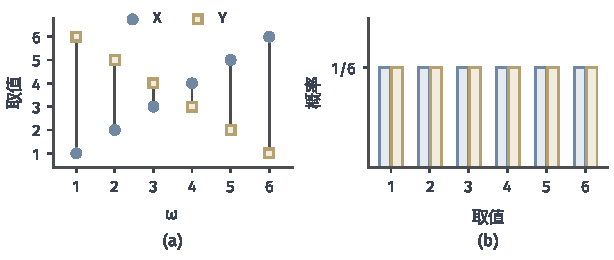
\includegraphics[width=104mm]{figures/07-probability/01-elementary-probability/matplotlib/rvd-same-law/figure.pdf}
  \caption{分布相同而取值不同。公平骰子上，$X(\omega)=\omega$（蓝点）与$Y(\omega)=7-\omega$（黄框）。(a)每个结果上两者的取值，竖线连接同一结果的两个值，没有一个结果使二者相等；(b)两者取$1,\dots,6$的概率都是$1/6$。}
  \label{fig:rvd-same-law}
\end{BookInlineFigure}

若$P_X=P_Y$，即对所有$B$都有$\mathbb{P}(X\in B)=\mathbb{P}(Y\in B)$，就说$X$与$Y$\term{同分布}（identically distributed）。同分布只是说两个变量“单独看”无法区分，不是说它们相等。这个例子里$X+Y$恒等于$7$，但仅凭两个分布无法知道这一点：若把$Y$换成另一枚独立骰子的点数，两个分布照旧，$X+Y$却会取$2$到$12$之间的各种值。表~\ref{tab:rvd-three-objects}总结了三个对象的区别。

\begin{BookInlineTable}
  \centering
  \begin{tabular}{lll}
    \toprule
    对象 & 是什么 & 骰子中的例子\\
    \midrule
    随机变量$X$ & $\Omega$上的函数 & $X(\omega)=\omega$\\
    实现值$x$ & 一次试验得到的数 & 这次掷出$x=5$\\
    分布$P_X$ & 实轴子集上的概率 & 每个点数概率$1/6$\\
    \bottomrule
  \end{tabular}
  \caption{随机变量、实现值与分布。前者是规则，中者是一次结果，后者是取值的概率规律；$X$与$7-X$是两个不同的规则，分布却相同。}
  \label{tab:rvd-three-objects}
\end{BookInlineTable}

\paragraph{随机变量的函数}
有了随机变量$X$和实函数$g$，复合$g(X)$，即$\omega\mapsto g(X(\omega))$，仍是$\Omega$上的函数，因而仍是随机变量。前面的$Y=7-X$就是$g(x)=7-x$的情形。抽检中，若抽两件、次品数为$X$，则合格品数是$2-X$，也属于这种情形。

$g(X)$的分布可以只用$X$的分布求出。事件$\{g(X)\in B\}$就是$\{X\in g^{-1}(B)\}$，其中$g^{-1}(B)$是被$g$送进$B$的$x$组成的集合。$X$只取有限或可数个值时，这给出
\begin{equation}
  \mathbb{P}(g(X)=y)=\sum_{x:\,g(x)=y}\mathbb{P}(X=x),
  \label{eq:rvd-function-pmf}
\end{equation}
即把被$g$送到同一个$y$的那些$x$的概率加起来。

下面用公平骰子的点数演示，取$g(x)=(x-3)^{2}$。$X=1,\dots,6$分别被送到$4,1,0,1,4,9$，其中$1$和$4$各收到两个点数。由式~\eqref{eq:rvd-function-pmf}，$Z=(X-3)^{2}$取各值的概率是
\[
  \mathbb{P}(Z=0)=\tfrac16,\quad \mathbb{P}(Z=1)=\tfrac26,\quad \mathbb{P}(Z=4)=\tfrac26,\quad \mathbb{P}(Z=9)=\tfrac16 .
\]
计算中没有回到样本空间，只用了$X$取各值的概率。取值连续变化的变量经过函数后分布怎样变化，需要换元等工具，由第~\ref{chap:random-variable-transformations}章处理。


\section{分布函数}
\label{sec:rvd-distribution-functions}

分布要对许多集合给出概率。骰子只有六个取值，列一张表就够了；等待时间可以取任何非负实数，不可能把每个区间的概率逐一列出。能不能用一个实变量的函数记下全部信息？

\paragraph{累计到阈值的概率}
设想沿实轴从左向右移动一个阈值$x$，每到一处就问：取值不超过$x$的概率有多大？按质量的图景，这是阈值左侧（含阈值本身）累积的质量。阈值移动时，这个数只增不减，从$0$开始，最后到$1$。

\begin{definition}[分布函数]
\label{def:rvd-cdf}
随机变量$X$的\term{分布函数}（cumulative distribution function）定义为
\begin{equation}
  F_X(x)=\mathbb{P}(X\leq x),\qquad x\in\mathbb{R}.
  \label{eq:rvd-cdf}
\end{equation}
\end{definition}

分布函数对每个实数$x$都有定义，不论$X$实际取哪些值。只要知道它，左开右闭区间的概率就能算出。设$a<b$，事件$\{X\leq b\}$是互斥的$\{X\leq a\}$与$\{a<X\leq b\}$之并，由可加性
\[
  \mathbb{P}(X\leq b)=\mathbb{P}(X\leq a)+\mathbb{P}(a<X\leq b),
\]
移项得到
\begin{equation}
  \mathbb{P}(a<X\leq b)=F_X(b)-F_X(a).
  \label{eq:rvd-interval}
\end{equation}
区间取左开右闭，正好与定义中的“$\leq$”配套：$\{X\leq a\}$含$a$，减去之后右边的区间就不含$a$。

\paragraph{抽检中的次品数}
一批$5$件产品中有$2$件次品，不放回地随机抽取$2$件，记次品数为$X$。按第~\ref{chap:classical-probability}章的计数，无序抽法共$\binom52=10$种，等可能。两件都合格有$\binom32=3$种，一件次品一件合格有$2\times3=6$种，两件都是次品有$1$种。于是
\[
  \mathbb{P}(X=0)=0.3,\quad \mathbb{P}(X=1)=0.6,\quad \mathbb{P}(X=2)=0.1 .
\]

现在让阈值$x$扫过实轴。$x<0$时没有任何可能取值不超过$x$；$0\leq x<1$时只有取值$0$满足；$1\leq x<2$时取值$0$和$1$满足；$x\geq2$时全部满足。所以
\begin{equation}
  F_X(x)=\begin{cases}
    0,&x<0,\\
    0.3,&0\leq x<1,\\
    0.9,&1\leq x<2,\\
    1,&x\geq 2.
  \end{cases}
  \label{eq:rvd-inspection-cdf}
\end{equation}
图~\ref{fig:rvd-inspection-cdf}以$x=1.5$为例：(a)中红线左侧的柱子是被累计的质量，(b)中红点是它们的和$F_X(1.5)=0.9$。

\begin{BookInlineFigure}
  \centering
  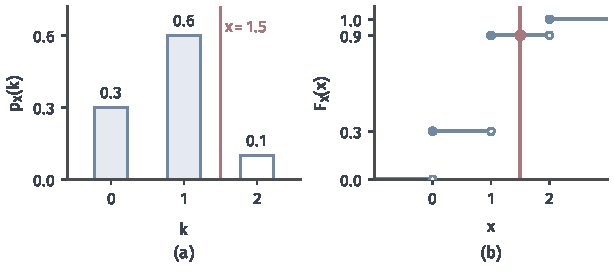
\includegraphics[width=104mm]{figures/07-probability/01-elementary-probability/matplotlib/rvd-inspection-cdf/figure.pdf}
  \caption{抽检次品数$X$的分布函数。(a)$X$取$0,1,2$的概率，红线是阈值$x=1.5$，左侧浅蓝柱被累计，右侧白柱不计；(b)分布函数，实心点是函数值，空心点是从左侧逼近的极限。红点$F_X(1.5)=0.3+0.6=0.9$。}
  \label{fig:rvd-inspection-cdf}
\end{BookInlineFigure}

$F_X$是阶梯函数：在两个可能取值之间，阈值移动不会越过新的质量，函数保持水平；阈值越过一个可能取值时，函数跳升，跳升的高度正是该处的概率。注意每个台阶的左端是实心点：$F_X(1)=0.9$，因为$\{X\leq1\}$包含$X=1$。

\paragraph{等待时间}
等待时间$T$（单位：分钟）不能列表，我们直接用分布函数给出模型：
\begin{equation}
  F_T(t)=\begin{cases}0,&t<0,\\1-\mathrm{e}^{-t},&t\geq0.\end{cases}
  \label{eq:rvd-waiting-cdf}
\end{equation}
它等价于规定“等待超过$t$分钟的概率是$\mathrm{e}^{-t}$”，等待越久越罕见。为什么这种形式适合描述等待，留到第~\ref{chap:common-distributions}章说明，这里只把它当作给定的模型。由式~\eqref{eq:rvd-interval}，等待$1$到$2$分钟的概率是
\[
  \mathbb{P}(1<T\leq2)=(1-\mathrm{e}^{-2})-(1-\mathrm{e}^{-1})=\mathrm{e}^{-1}-\mathrm{e}^{-2}\approx0.2325 .
\]
等待超过$2$分钟的概率是$1-F_T(2)=\mathrm{e}^{-2}\approx0.1353$。

这条曲线处处连续，没有跳跃。与抽检的阶梯对比，可以预料：跳跃对应集中在单点的概率，而等待时间没有哪一个具体时刻带有正概率。下面把这个预料写成定理。

\paragraph{分布函数的性质}
阶梯函数和连续曲线看起来很不同，但它们有共同的骨架：单调不减，在每一点从右侧连续，两端分别趋于$0$和$1$，跳跃高度等于单点概率。先对取有限或可数个值的随机变量证明这些性质；用密度给出的模型在第~\ref{sec:rvd-mass-density}节核验，一般情形的依据在第~\ref{chap:probability-spaces}章给出。

设$X$只取值$x_1,x_2,\dots$（有限个或可数个，互不相同），记$q_i=\mathbb{P}(X=x_i)$，这些数非负，总和为$1$。取有限个值时，每个事件的概率就是其中各取值概率之和；取可数个值时，我们把这一点作为模型的规定：$\mathbb{P}(X\in B)$等于$x_i\in B$的那些$q_i$之和。非负项级数可以任意重排和分组而和不变，所以这样规定的概率同样满足可加性。于是
\[
  F_X(x)=\sum_{i:\,x_i\leq x}q_i .
\]

\begin{theorem}[分布函数的性质]
\label{thm:rvd-cdf-properties}
设随机变量$X$只取有限或可数个值，$F=F_X$。则
\begin{enumerate}
  \item 单调不减：$x<y$时$F(x)\leq F(y)$；
  \item 右连续：对每个$x$，$\lim_{h\downarrow0}F(x+h)=F(x)$；
  \item 两端极限：$\lim_{x\to-\infty}F(x)=0$，$\lim_{x\to+\infty}F(x)=1$；
  \item 左极限存在，并且
  \begin{equation}
    F(x^{-})=\lim_{h\downarrow0}F(x-h)=\mathbb{P}(X<x),\qquad F(x)-F(x^{-})=\mathbb{P}(X=x).
    \label{eq:rvd-jump}
  \end{equation}
\end{enumerate}
\end{theorem}

\begin{proof}
单调性：$x<y$时，满足$x_i\leq x$的下标都满足$x_i\leq y$，后者的和多出一些非负项，所以$F(x)\leq F(y)$。

其余三条都依靠同一个估计：总和为$1$的级数，尾部可以任意小。给定$\varepsilon>0$，取$N$使
\[
  \sum_{i>N}q_i<\varepsilon .
\]
这时只有前$N$个取值可能带来不小的概率，而有限个点总是离给定的点有正的距离。

右连续：$F(x+h)-F(x)$是落在$(x,x+h]$里的那些$q_i$之和。前$N$个取值中大于$x$的有有限个，记它们到$x$的最小距离为$\delta>0$（若没有这样的取值，取$\delta=1$）。当$0<h<\delta$时，前$N$个取值都不在$(x,x+h]$中，于是
\[
  0\leq F(x+h)-F(x)\leq\sum_{i>N}q_i<\varepsilon .
\]

两端极限：当$x$小于$x_1,\dots,x_N$中的最小者时，$F(x)$只含下标大于$N$的项，所以$F(x)<\varepsilon$。当$x$不小于其中最大者时，$F(x)$包含前$N$项，所以
\[
  F(x)\geq\sum_{i\leq N}q_i>1-\varepsilon .
\]
又$0\leq F\leq1$，两端极限分别为$0$和$1$。

左极限：$F(x)-F(x-h)$是落在$(x-h,x]$里的$q_i$之和，它等于$\mathbb{P}(X=x)$加上落在$(x-h,x)$里的那些项。与右连续的论证相同，$h$足够小时后者小于$\varepsilon$，所以
\[
  \lim_{h\downarrow0}\bigl(F(x)-F(x-h)\bigr)=\mathbb{P}(X=x).
\]
移项即得式~\eqref{eq:rvd-jump}中左极限的值$F(x)-\mathbb{P}(X=x)=\mathbb{P}(X<x)$。
\end{proof}

右连续而不一定左连续，原因在于“$\leq$”包含阈值本身。图~\ref{fig:rvd-jump-limits}放大了抽检例子在$x=1$处的跳跃。从右侧逼近时，阈值$1+1/n$与$1$之间没有可能取值，累计的总是$X=0$和$X=1$两份质量，函数值恒为$0.9=F(1)$。从左侧逼近时，阈值$1-1/n$还没有越过$1$，累计的只有$X=0$那一份，极限是$0.3$。两者之差$0.6$就是$X=1$的概率。

\begin{BookInlineFigure}
  \centering
  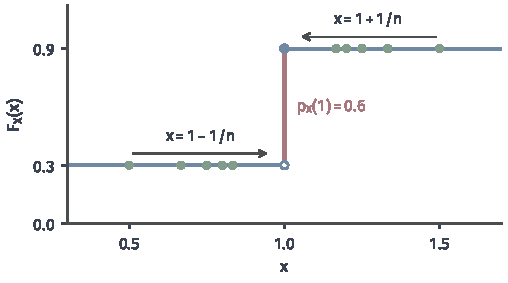
\includegraphics[width=86mm]{figures/07-probability/01-elementary-probability/matplotlib/rvd-jump-limits/figure.pdf}
  \caption{抽检次品数的分布函数在$x=1$处的两侧极限。绿点是阈值$1+1/n$与$1-1/n$（$n=2,\dots,6$）处的函数值：右侧一列恒为$0.9$，等于$F_X(1)$（实心点）；左侧一列恒为$0.3$，等于左极限（空心点）。红色竖线是跳跃高度$0.6=\mathbb{P}(X=1)$。}
  \label{fig:rvd-jump-limits}
\end{BookInlineFigure}

\paragraph{三条性质各管什么}
单调、右连续、两端极限这三条性质，每一条都排除了一类不可能是分布函数的函数。拿抽检例子对照，可以看清它们各自的作用。

单调不减保证区间概率非负：由式~\eqref{eq:rvd-interval}，$F(b)-F(a)$是概率，不能为负。右连续是“$\leq$”这一约定的结果。若改用$G(x)=\mathbb{P}(X<x)$记录累计概率，抽检例子给出
\[
  G(x)=\begin{cases}0,&x\leq0,\\0.3,&0<x\leq1,\\0.9,&1<x\leq2,\\1,&x>2,\end{cases}
\]
它在每个跳跃点取左侧的值，是左连续的。$G$包含的信息与$F_X$相同，只是约定不同；本书统一使用“$\leq$”，因此分布函数总是右连续的。

两端极限保证质量既不从左侧漏走，也不在右侧缺失。设某台设备收到请求后，以概率$1/2$会响应，响应前的等待按式~\eqref{eq:rvd-waiting-cdf}的规律分布；以概率$1/2$永不响应。由全概率公式，等待不超过$t$分钟的概率是
\[
  H(t)=\tfrac12\bigl(1-\mathrm{e}^{-t}\bigr),\qquad t\geq0,
\]
它单调、连续，$t\to\infty$时却只趋于$1/2$。缺少的一半质量在“无穷远处”，响应时间不是一个实数值的随机变量。要用实值随机变量描述这台设备，就得另外记录“是否响应”，或者给等待设一个上限。

\paragraph{累计事件往往更好算}
第~\ref{sec:rvd-random-variables}节求两枚骰子较大点数$M$的概率时，先数的是$\{M\leq m\}$，用的正是分布函数。对一般的实数$x$，$\{M\leq x\}$要求两个点数都不超过$x$，所以
\[
  F_M(x)=\frac{\lfloor x\rfloor^{2}}{36},\qquad 0\leq x<6,
\]
$x<0$时为$0$，$x\geq6$时为$1$，其中$\lfloor x\rfloor$是不超过$x$的最大整数。再由式~\eqref{eq:rvd-jump}读跳跃高度，就回到$\mathbb{P}(M=m)=(2m-1)/36$。最大值、最小值这类变量，“都不超过”或“都超过”的事件可以直接计数，单点事件反而要分情形，这时先求分布函数更方便。

\paragraph{各种区间的概率}
有了左极限，端点开闭不同的区间都能用分布函数表示。式~\eqref{eq:rvd-jump}给出$\mathbb{P}(X<x)=F(x^{-})$，与式~\eqref{eq:rvd-interval}同样相减，得到表~\ref{tab:rvd-intervals}。它们的规律是：区间包含左端点$a$时减去$F(a^{-})$，不含时减去$F(a)$；包含右端点$b$时用$F(b)$，不含时用$F(b^{-})$。

\begin{BookInlineTable}
  \centering
  \begin{tabular}{ll@{\qquad}ll}
    \toprule
    事件 & 概率 & 事件 & 概率\\
    \midrule
    $a<X\leq b$ & $F(b)-F(a)$ & $a\leq X\leq b$ & $F(b)-F(a^{-})$\\
    $a<X<b$ & $F(b^{-})-F(a)$ & $a\leq X<b$ & $F(b^{-})-F(a^{-})$\\
    $X>a$ & $1-F(a)$ & $X\geq a$ & $1-F(a^{-})$\\
    \bottomrule
  \end{tabular}
  \caption{用分布函数表示区间概率，其中$a<b$，$F=F_X$，$F(a^{-})$是左极限。$F$在$a$、$b$处连续时，左右两列相同。}
  \label{tab:rvd-intervals}
\end{BookInlineTable}

在抽检例子中端点会造成差别。由式~\eqref{eq:rvd-inspection-cdf}，$F(1^{-})=0.3$，所以
\[
  \mathbb{P}(1\leq X\leq2)=F(2)-F(1^{-})=1-0.3=0.7,
\]
而
\[
  \mathbb{P}(1<X\leq2)=F(2)-F(1)=1-0.9=0.1 .
\]
前者包含$X=1$的$0.6$，后者不包含。等待时间的分布函数处处连续，左极限等于函数值，端点开闭不影响结果：
\[
  \mathbb{P}(1\leq T\leq2)=\mathbb{P}(1<T\leq2)\approx0.2325 .
\]

\paragraph{分布函数确定分布}
上面的计算表明，区间及其有限并的概率都能由分布函数得到，因此两个随机变量的分布函数相同，它们在这些集合上的概率就相同。反过来还有一个更强的事实：任何单调不减、右连续、两端极限为$0$和$1$的函数，都是某个随机变量的分布函数。这一结论需要构造一般的概率模型，在第~\ref{chap:probability-spaces}章证明。它意味着定理~\ref{thm:rvd-cdf-properties}的前三条性质恰好刻画了所有分布函数，本部分可以放心地直接用一个满足这三条的函数来规定模型，就像式~\eqref{eq:rvd-waiting-cdf}所做的那样。


\section{概率质量与密度}
\label{sec:rvd-mass-density}

分布函数对所有随机变量都适用，但用它算概率并不总是最直接。抽检的次品数，一张三格的表就说完了；等待时间的分布函数是累计量，问“等待在$1.5$分钟附近有多集中”时，还得从它的变化率读出来。本节为两类常见情形各给一种更直接的表示：取值可以一一列出时，记录每个取值的概率；取值连续铺开时，记录单位长度上的概率。

\paragraph{概率质量函数}
骰子点数、次品数、首次成功前的试验次数，都只取有限或可数个值。对这类变量，最自然的描述是逐个列出取值和概率，就像上一节证明定理~\ref{thm:rvd-cdf-properties}时所用的表。

\begin{definition}[概率质量函数]
\label{def:rvd-pmf}
若存在有限或可数的集合$\{x_1,x_2,\dots\}$，使$X$只在其中取值，即$\sum_i\mathbb{P}(X=x_i)=1$，就称$X$为\term{离散随机变量}（discrete random variable）。函数
\begin{equation}
  p_X(x)=\mathbb{P}(X=x),\qquad x\in\mathbb{R}
  \label{eq:rvd-pmf}
\end{equation}
称为$X$的\term{概率质量函数}（probability mass function）。集合$\{x:p_X(x)>0\}$称为它的\term{支撑}（support）。
\end{definition}

质量函数满足两条：$p_X(x)\geq0$，且在支撑上的总和为$1$。按上一节对可数取值的约定，任何集合的概率都是其中各点质量之和：
\begin{equation}
  \mathbb{P}(X\in B)=\sum_{x_i\in B}p_X(x_i).
  \label{eq:rvd-pmf-sum}
\end{equation}
反过来，任给有限或可数个点和一组非负、总和为$1$的数，都能这样规定一个离散分布。离散分布的计算因此就是求和。

质量函数与分布函数互相确定。由式~\eqref{eq:rvd-pmf-sum}取$B=(-\infty,x]$，得到
\begin{equation}
  F_X(x)=\sum_{x_i\leq x}p_X(x_i);
  \label{eq:rvd-pmf-to-cdf}
\end{equation}
反方向，由式~\eqref{eq:rvd-jump}，$p_X(x)=F_X(x)-F_X(x^{-})$，即分布函数在$x$处的跳跃高度。图~\ref{fig:rvd-inspection-cdf}的两幅子图正是同一分布的两种表示。

\paragraph{可数个取值：首次掷出六点}
反复掷一枚公平骰子，记第一次出现六点时已掷的次数为$N$。事件$\{N=k\}$是“前$k-1$次都不是六点、第$k$次是六点”。各次投掷相互独立，由第~\ref{chap:classical-probability}章的乘法规则，
\begin{equation}
  p_N(k)=\Bigl(\frac56\Bigr)^{k-1}\frac16,\qquad k=1,2,3,\dots
  \label{eq:rvd-first-six}
\end{equation}
$N$可以取任意正整数，支撑是可数无限集。

先核对总质量。这是首项$1/6$、公比$5/6$的几何级数，
\[
  \sum_{k=1}^{\infty}\Bigl(\frac56\Bigr)^{k-1}\frac16=\frac16\cdot\frac{1}{1-5/6}=1 .
\]
再由式~\eqref{eq:rvd-pmf-to-cdf}求分布函数。对正整数$k$，前$k$项的部分和是
\[
  F_N(k)=\frac16\cdot\frac{1-(5/6)^{k}}{1-5/6}=1-\Bigl(\frac56\Bigr)^{k}.
\]
它也可以直接看出：$\{N>k\}$就是前$k$次都不是六点，概率为$(5/6)^{k}$。

图~\ref{fig:rvd-first-six}画出了质量函数和分布函数。分布函数在每个正整数处跳跃，跳跃无穷多次，却始终没有到达$1$；它与$1$的距离是尚未累计的尾部质量。例如掷了$10$次仍未出现六点的概率是$(5/6)^{10}\approx0.1615$，这正是定理~\ref{thm:rvd-cdf-properties}证明中“级数尾部可以任意小”的具体样子。

\begin{BookInlineFigure}
  \centering
  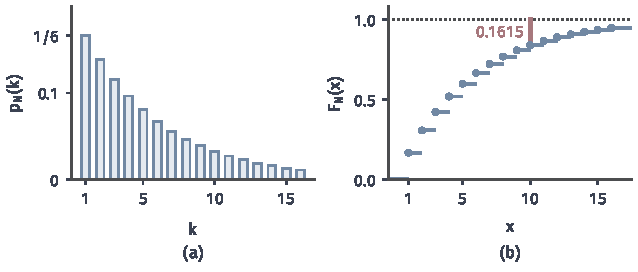
\includegraphics[width=108mm]{figures/07-probability/01-elementary-probability/matplotlib/rvd-first-six/figure.pdf}
  \caption{首次掷出六点所需次数$N$。(a)质量函数$p_N(k)=(5/6)^{k-1}/6$，只画出$k\leq16$；(b)分布函数$F_N$，在每个正整数处跳跃，点线是高度$1$。红线是$x=10$处尚未累计的质量$(5/6)^{10}\approx0.1615$。}
  \label{fig:rvd-first-six}
\end{BookInlineFigure}

\paragraph{核对一张概率表}
给出一张表时，要检查非负、总和为$1$，并说明支撑。设$X$取正整数，$p_X(k)=c/(k(k+1))$，常数$c$待定。把每一项拆成两个分数之差，部分和中间各项依次抵消：
\[
  \sum_{k=1}^{n}\frac{1}{k(k+1)}=\sum_{k=1}^{n}\Bigl(\frac1k-\frac1{k+1}\Bigr)=1-\frac1{n+1}.
\]
令$n\to\infty$，级数和为$1$，所以$c=1$。用同样的抵消，$\mathbb{P}(X\geq5)=1/5$，$F_X(k)=k/(k+1)$。这张表下一节还会用到：它的尾部衰减得很慢。

\paragraph{密度：单位长度上的概率}
等待时间的分布函数处处连续。对任意$t$和$h>0$，$\{T=t\}\subseteq\{t-h<T\leq t\}$，所以$\mathbb{P}(T=t)\leq F_T(t)-F_T(t-h)$，令$h\to0$即得$\mathbb{P}(T=t)=0$。每个单点的概率都是$0$，质量函数恒为零，提供不了任何信息。概率并没有消失，只是不再集中在一个个点上，而是像一根粗细不均的细棒上的质量那样沿实轴连续铺开。描述细棒，我们用线密度，即单位长度上的质量；某一段的质量是线密度在这一段上的积分。

先看一个能直接算出“单位长度上的概率”的例子。在半径为$1$的圆盘内随机取一点，规定点落在任一区域的概率等于该区域面积与圆盘面积$\pi$之比。记点到圆心的距离为$R$。$\{R\leq r\}$是半径$r$的小圆盘（图~\ref{fig:rvd-disk-radius}(a)），所以
\[
  F_R(r)=\frac{\pi r^{2}}{\pi}=r^{2},\qquad 0\leq r\leq1 .
\]
$r<0$时$F_R(r)=0$，$r>1$时$F_R(r)=1$。

\begin{BookInlineFigure}
  \centering
  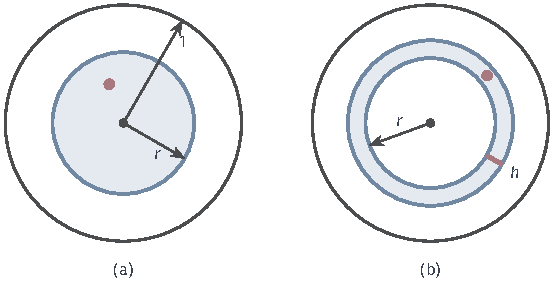
\includegraphics[width=94mm]{figures/07-probability/01-elementary-probability/tikz/rvd-disk-radius/figure.pdf}
  \caption{单位圆盘内随机取点（红点），$R$是它到圆心的距离。(a)事件$\{R\leq r\}$是浅蓝的小圆盘，概率为面积比$r^{2}$；(b)事件$\{r<R\leq r+h\}$是宽$h$的圆环，面积$\pi(2rh+h^{2})$，概率约为$2rh$。圆环越靠外越长，所以同样宽度的圆环外侧概率更大。}
  \label{fig:rvd-disk-radius}
\end{BookInlineFigure}

现在取一个宽$h$的圆环$\{r<R\leq r+h\}$（图~\ref{fig:rvd-disk-radius}(b)）。由式~\eqref{eq:rvd-interval}，
\[
  \mathbb{P}(r<R\leq r+h)=(r+h)^{2}-r^{2}=2rh+h^{2}.
\]
除以宽度$h$，得到这一段上平均每单位长度的概率：
\[
  \frac{\mathbb{P}(r<R\leq r+h)}{h}=2r+h .
\]
令$h\to0$，极限是$2r$。这就是$R$在$r$处的“单位长度上的概率”。

图~\ref{fig:rvd-density-histogram}把这个比值画成柱：每根柱的面积等于对应区间的概率，柱高是概率除以宽度。宽度从$0.25$缩小到$0.05$，柱顶越来越贴近直线$2r$。点在圆盘内是“均匀”取的，$R$却不均匀：离圆心越远，同样宽度的圆环越长，分到的概率越多。

\begin{BookInlineFigure}
  \centering
  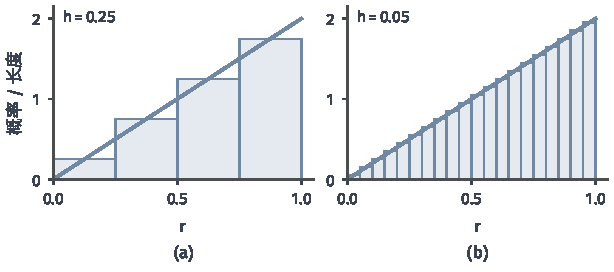
\includegraphics[width=104mm]{figures/07-probability/01-elementary-probability/matplotlib/rvd-density-histogram/figure.pdf}
  \caption{圆盘半径$R$的单位长度概率。浅蓝柱的宽度为$h$，高度为$\mathbb{P}(r<R\leq r+h)/h=2r+h$，面积就是该段的概率；蓝线是极限$2r$。(a)$h=0.25$；(b)$h=0.05$，柱顶与直线的差距缩小为$h$。}
  \label{fig:rvd-density-histogram}
\end{BookInlineFigure}

把这种描述作为定义：不再从分布函数出发求变化率，而是直接用一个函数的积分规定区间概率。

\begin{definition}[概率密度函数]
\label{def:rvd-density}
若存在非负函数$f_X$，使$\int_{-\infty}^{\infty}f_X(x)\,\mathrm{d}x=1$，并且对一切$a<b$都有
\begin{equation}
  \mathbb{P}(a<X\leq b)=\int_{a}^{b}f_X(x)\,\mathrm{d}x,
  \label{eq:rvd-density}
\end{equation}
就称$X$有\term{概率密度函数}（probability density function）$f_X$，简称密度。其中$a$可以取$-\infty$，$b$可以取$+\infty$，积分可以是反常积分。
\end{definition}

这里的积分是卷一意义下的黎曼积分，在无穷区间或被积函数无界时按反常积分理解，可参考\BookChapterRef{chap:univariate-integration}{卷一第7章“一元函数的积分”}。密度为正的范围称为它的支撑，例如$R$的支撑是$[0,1]$，等待时间的支撑是$[0,\infty)$。取$a=-\infty$，定义直接给出分布函数是密度的累计：
\begin{equation}
  F_X(x)=\int_{-\infty}^{x}f_X(t)\,\mathrm{d}t .
  \label{eq:rvd-cdf-from-density}
\end{equation}

\paragraph{密度模型的分布函数}
上一节对离散变量证明了分布函数的性质，现在对有密度的变量核验同样的性质，并看清单点概率为什么都是零。

\begin{theorem}[有密度时的分布函数]
\label{thm:rvd-density-cdf}
设$X$有密度$f_X$。则$F_X$单调不减、处处连续，$\lim_{x\to-\infty}F_X(x)=0$，$\lim_{x\to+\infty}F_X(x)=1$，并且对每个$x$都有$\mathbb{P}(X=x)=0$。若$f_X$在$x_0$处连续，则$F_X$在$x_0$处可导，且
\begin{equation}
  F_X'(x_0)=f_X(x_0).
  \label{eq:rvd-density-derivative}
\end{equation}
\end{theorem}

\begin{proof}
单调性来自被积函数非负：$x<y$时$F_X(y)-F_X(x)=\int_x^yf_X\geq0$。两端极限是反常积分$\int_{-\infty}^{\infty}f_X=1$收敛的定义：上限趋于$-\infty$时积分趋于$0$，趋于$+\infty$时积分趋于$1$。

连续性要证明$h\to0$时$\int_x^{x+h}f_X\to0$（$h<0$时理解为$-\int_{x+h}^{x}f_X$）。若$f_X$在$x$附近有界，设$\lvert f_X\rvert\leq K$，则这个积分的绝对值不超过$K\lvert h\rvert$，趋于$0$。若$f_X$在$x$附近无界，$x$是反常积分的瑕点，而反常积分收敛的定义正是积分上限（或下限）趋于瑕点时积分有极限，这个极限就是$F_X(x)$，所以积分同样趋于$0$。

单点概率：对$h>0$，$\{X=x\}\subseteq\{x-h<X\leq x\}$，于是
\[
  0\leq\mathbb{P}(X=x)\leq F_X(x)-F_X(x-h).
\]
由连续性，右边随$h\to0$趋于$0$，所以$\mathbb{P}(X=x)=0$。最后，$f_X$在$x_0$处连续时，式~\eqref{eq:rvd-density-derivative}是微积分基本定理对积分上限函数的结论。
\end{proof}

于是有密度的变量取任何一个具体值的概率都是$0$，而它每次总会取到某个值。这并不矛盾：实轴上有不可数多个点，概率是在区间上累计起来的，不是逐点相加起来的。“概率为零”与“不可能”在这里分开了：$\{T=1\}$是可能发生的事件，概率却为零。实际计算中的直接后果是端点开闭不再重要：
\[
  \mathbb{P}(a<X\leq b)=\mathbb{P}(a\leq X\leq b)=\mathbb{P}(a<X<b)=\int_a^bf_X(x)\,\mathrm{d}x .
\]

\paragraph{等待时间的密度}
式~\eqref{eq:rvd-waiting-cdf}的分布函数在$t\neq0$处可导，导数在$t<0$时为$0$，在$t>0$时为$\mathrm{e}^{-t}$。下面会说明，这样的分布函数由导数给出密度：
\[
  f_T(t)=\begin{cases}0,&t<0,\\\mathrm{e}^{-t},&t\geq0.\end{cases}
\]
图~\ref{fig:rvd-waiting-density-cdf}用两种方式表示同一个概率$\mathbb{P}(1<T\leq2)\approx0.2325$：在密度图中它是曲线下的面积，在分布函数图中它是两个函数值的高度差。密度越大的地方，分布函数上升越快。

\begin{BookInlineFigure}
  \centering
  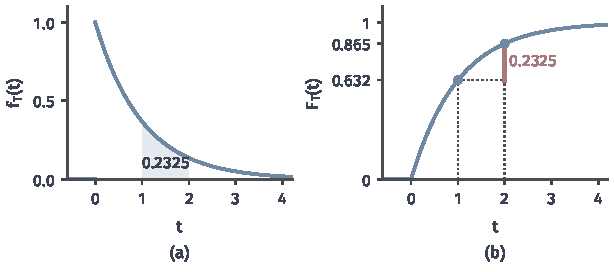
\includegraphics[width=104mm]{figures/07-probability/01-elementary-probability/matplotlib/rvd-waiting-density-cdf/figure.pdf}
  \caption{等待时间$T$的密度与分布函数。(a)密度$f_T(t)=\mathrm{e}^{-t}$（$t\geq0$），浅蓝面积是$\mathbb{P}(1<T\leq2)=\mathrm{e}^{-1}-\mathrm{e}^{-2}\approx0.2325$；(b)分布函数$F_T(t)=1-\mathrm{e}^{-t}$，同一概率是$t=2$与$t=1$处函数值之差（红线）。}
  \label{fig:rvd-waiting-density-cdf}
\end{BookInlineFigure}

\paragraph{由分布函数求密度}
定理~\ref{thm:rvd-density-cdf}说密度是分布函数的导数。反过来，什么时候能对分布函数求导得到密度？最常用的是下面这个充分条件。

\begin{theorem}[由分布函数求密度]
\label{thm:rvd-cdf-to-density}
设$F_X$处处连续，并且除有限个点$c_1<\dots<c_m$外连续可导，导数$F_X'$在每个开区间$(c_{k},c_{k+1})$上反常可积。令$f(x)=F_X'(x)$（在$c_k$处任意取非负值），则$f$是$X$的密度。
\end{theorem}

\begin{proof}
分布函数单调不减，所以导数$F_X'\geq0$，$f$非负。取$a<b$，在$a,b$之间插入落在其中的那些$c_k$，把$[a,b]$分成若干段。在每一段的内部，$F_X$连续可导，由Newton--Leibniz公式，$F_X$在段内两点之间的增量等于导数的积分；让两点趋于段端，$F_X$的连续性保证增量趋于整段的增量，积分按反常积分收敛到整段的积分。各段相加，得到
\[
  F_X(b)-F_X(a)=\int_a^bf(x)\,\mathrm{d}x .
\]
这就是式~\eqref{eq:rvd-density}。令$a\to-\infty$、$b\to+\infty$，由分布函数的两端极限得到$\int_{-\infty}^{\infty}f=1$。有限个点处的取值不影响积分。
\end{proof}

圆盘半径$R$满足条件：$F_R$连续，除$r=0,1$外可导，于是$f_R(r)=2r$（$0<r<1$），其余处为$0$，正是前面由圆环得到的极限。用它验算：
\[
  \mathbb{P}(0.5<R\leq1)=\int_{0.5}^{1}2r\,\mathrm{d}r=1-0.25=0.75 .
\]
从分布函数直接算是$F_R(1)-F_R(0.5)=0.75$，两者一致。条件中的“连续”不能去掉：抽检次品数的分布函数除三个点外导数都是零，按导数得到的“密度”积分为$0$，丢掉了全部质量。第~\ref{sec:rvd-representation-limits}节还会看到，即使分布函数连续，也可能求不出密度。

\paragraph{密度值不是概率}
密度的单位是“概率每单位长度”，它的值本身不是任何事件的概率。若$f_X$在$x$处连续，由积分中值定理，存在$\xi_h\in[x,x+h]$使
\[
  \mathbb{P}(x<X\leq x+h)=f_X(\xi_h)\,h\approx f_X(x)\,h .
\]
所以只有乘上一小段长度，密度才变成概率。密度的值可以大于$1$，甚至可以无界，只要曲线下的总面积是$1$。

图~\ref{fig:rvd-density-values}给出三个例子。(a)在$(0,1/2)$上$f(x)=2$，其余处为$0$，总面积$2\times\frac12=1$，而
\[
  \mathbb{P}(0.1<X\leq0.3)=2\times0.2=0.4 .
\]
(b)在$(0,1)$上$f(x)=6x(1-x)$，最大值$f(1/2)=1.5$，下面还会用它演示怎样核对密度。(c)在$(0,1]$上$f(x)=1/(2\sqrt{x})$，在$0$附近无界，但反常积分收敛，分布函数是$F(x)=\sqrt{x}$（$0\leq x\leq1$），于是
\[
  \mathbb{P}(X\leq\tfrac14)=\sqrt{1/4}=\tfrac12 .
\]

\begin{BookInlineFigure}
  \centering
  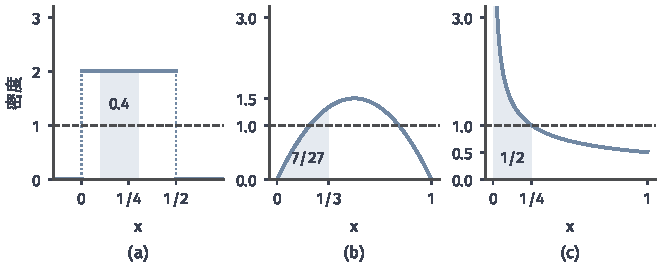
\includegraphics[width=112mm]{figures/07-probability/01-elementary-probability/matplotlib/rvd-density-values/figure.pdf}
  \caption{密度的高度不是概率。虚线是高度$1$，浅蓝面积是所标的概率。(a)$(0,1/2)$上的常数密度$2$，$\mathbb{P}(0.1<X\leq0.3)=0.4$；(b)$6x(1-x)$，最大值$1.5$，$\mathbb{P}(X\leq1/3)=7/27$；(c)$1/(2\sqrt{x})$在$0$附近无界，$\mathbb{P}(X\leq1/4)=1/2$。}
  \label{fig:rvd-density-values}
\end{BookInlineFigure}

密度值还依赖于单位。等待时间以分钟计时密度在$0$处等于$1$；改以小时计，$H=T/60$，于是对$s\geq0$，
\[
  \mathbb{P}(H\leq s)=\mathbb{P}(T\leq60s)=1-\mathrm{e}^{-60s}.
\]
求导得
\[
  f_H(s)=60\,\mathrm{e}^{-60s},\qquad s\geq0,
\]
在$0$处等于$60$。同一事件的概率不随单位改变，单位长度上的概率却要按长度单位换算。

\paragraph{核对一个函数是不是密度}
给出候选密度时，要核对三件事：在支撑上非负，总积分为$1$，支撑写清楚。设$f(x)=c\,x(1-x)$（$0<x<1$），其余处为$0$。在$(0,1)$上$x(1-x)>0$，非负性只要求$c>0$。归一化要求
\[
  c\int_0^1x(1-x)\,\mathrm{d}x=c\Bigl(\frac12-\frac13\Bigr)=\frac c6=1,
\]
所以$c=6$，这就是图~\ref{fig:rvd-density-values}(b)。它的分布函数是
\[
  F(x)=\int_0^x6t(1-t)\,\mathrm{d}t=3x^{2}-2x^{3},\qquad 0\leq x\leq1,
\]
所以$\mathbb{P}(X\leq1/3)=3/9-2/27=7/27\approx0.259$。

支撑不能随意扩大。若把同一公式用在$(0,2)$上，$1<x<2$时$x(1-x)<0$，无论$c$取什么正数都违反非负性；把公式写成“$f(x)=6x(1-x)$”而不写支撑，读者就无从判断它在区间外是什么。

\paragraph{从细格上的质量到密度}
质量与密度的关系可以通过把格子越分越细看出来。设$X_n$以概率$1/n$取$1/n,2/n,\dots,n/n$中的每一个值，相邻取值相距$1/n$。每一点的质量$1/n$随$n$增大趋于$0$，但质量除以格宽始终是
\[
  \frac{1/n}{1/n}=1 .
\]
分布函数是$F_{X_n}(x)=\lfloor nx\rfloor/n$（$0\leq x\leq1$），它与$x$的差不超过$1/n$。

当$n\to\infty$时，阶梯越来越密、台阶越来越矮，分布函数逼近$F(x)=x$，这正是$(0,1)$上常数密度$1$的分布函数。质量函数的值趋于零，提供不了极限的信息；分布函数和“质量除以格宽”却都有好的极限。所以比较离散与连续的模型时，要拿分布函数比，或者拿“质量/格宽”与密度比，不能拿单点质量与密度值比。分布怎样在这种意义下逼近，在第~\ref{chap:random-variable-convergence}章系统研究。

\paragraph{密度只在积分意义下确定}
改变$f_X$在有限个点处的值，所有区间上的积分都不变，因而规定的是同一个分布。所以“$X$的密度”实际上指一族只在有限个点处不同的函数，我们总选其中最方便的一个，例如在支撑的端点处取什么值都可以。与此不同，质量函数在每一点的值都有意义，改动任何一点都会改变分布。这也说明密度在单点上的值不能单独解释，只有它在小区间上的平均才对应概率。

表~\ref{tab:rvd-mass-vs-density}对比了两种表示。

\begin{BookInlineTable}
  \centering
  \begin{tabular}{lll}
    \toprule
    & 质量函数$p_X$ & 密度$f_X$\\
    \midrule
    区间概率 & 对取值求和 & 在区间上积分\\
    函数值 & 单点概率，不超过$1$ & 单位长度的概率，可大于$1$\\
    单点概率 & $p_X(x)$ & 恒为$0$\\
    分布函数 & 阶梯，跳跃高度为$p_X$ & 连续，导数为$f_X$\\
    端点开闭 & 可能改变结果 & 不影响结果\\
    改动一点的值 & 改变分布 & 不改变分布\\
    \bottomrule
  \end{tabular}
  \caption{概率质量函数与概率密度函数的对比。两者都要求非负、总量为$1$；区别在于质量集中在可数个点上，还是沿实轴连续铺开。}
  \label{tab:rvd-mass-vs-density}
\end{BookInlineTable}

习惯上把有密度的分布称为连续分布，把离散随机变量的分布称为离散分布。“连续分布”这个名字只说明分布函数连续；第~\ref{sec:rvd-representation-limits}节会看到，分布函数连续并不保证密度存在。


\section{分位数}
\label{sec:rvd-quantiles}

窗口想承诺“九成顾客的等待不超过某个时长”，这个时长应当定为多少？分布函数回答的是“给定阈值，累计概率多大”，现在的问题方向相反：给定累计概率$p$，求阈值$x$。

\paragraph{反解分布函数}
对等待时间，$F_T(t)=1-\mathrm{e}^{-t}$在$t\geq0$上连续且严格递增，方程$F_T(t)=p$对每个$0<p<1$恰有一个解：
\[
  1-\mathrm{e}^{-t}=p\quad\Longleftrightarrow\quad t=-\ln(1-p).
\]
取$p=0.9$，得$t=\ln10\approx2.303$分钟：九成顾客等待不超过约$2.3$分钟。

离散变量就没有这么顺利。公平骰子的分布函数在$[2,3)$上等于$1/3$，在$3$处跳到$1/2$，方程$F(x)=0.4$根本没有解；而$F(x)=1/2$对$[3,4)$中的每个$x$都成立，解有无穷多个。跳跃使某些$p$取不到，平台使某些$p$的解不唯一。我们需要一个对任何分布函数都有意义的约定。

自然的想法是不再要求“恰好等于$p$”，而是找累计概率首次达到$p$的位置。$p=0.4$时，阈值从左向右移动，到$x=3$时累计概率从$1/3$跳到$1/2$，第一次不小于$0.4$，所以取$3$。$p=1/2$时，累计概率在$x=3$处第一次达到$1/2$，平台上的其余点都在它右边，所以也取$3$。

\begin{definition}[分位数]
\label{def:rvd-quantile}
设$F$是随机变量$X$的分布函数，$0<p<1$。称
\begin{equation}
  Q(p)=\inf\{x\in\mathbb{R}:F(x)\geq p\}
  \label{eq:rvd-quantile}
\end{equation}
为$X$的$p$\term{分位数}（quantile），函数$p\mapsto Q(p)$称为\term{分位数函数}（quantile function）。$Q(1/2)$称为\term{中位数}（median），$Q(1/4)$与$Q(3/4)$分别称为下、上\term{四分位数}（quartile）。
\end{definition}

\paragraph{分位数与分布函数的对应}
分位数用到的只是分布函数的三条性质：单调不减、右连续、两端极限为$0$和$1$。前面各节的离散模型和密度模型都满足它们。下面的引理把下确界化成一个可以直接使用的等价关系。

\begin{lemma}[分位数的等价刻画]
\label{lem:rvd-quantile-galois}
设$0<p<1$。则$Q(p)$是有限实数，并且对一切实数$x$，
\begin{equation}
  Q(p)\leq x\quad\Longleftrightarrow\quad p\leq F(x).
  \label{eq:rvd-quantile-galois}
\end{equation}
\end{lemma}

\begin{proof}
记$A_p=\{x:F(x)\geq p\}$。因为$F(x)\to1>p$（$x\to+\infty$），$A_p$非空；因为$F(x)\to0<p$（$x\to-\infty$），$A_p$有下界。所以下确界$Q(p)$是有限实数。

$A_p$向右封闭：若$x\in A_p$且$y>x$，由单调性$F(y)\geq F(x)\geq p$，所以$y\in A_p$。再看下确界本身是否属于$A_p$。取$A_p$中的点列$x_n$从右侧趋于$Q(p)$，由右连续，
\[
  F(Q(p))=\lim_{n\to\infty}F(x_n)\geq p .
\]
所以$Q(p)\in A_p$，从而$A_p=[Q(p),\infty)$。“$x\in A_p$”就是“$p\leq F(x)$”，“$x\in[Q(p),\infty)$”就是“$Q(p)\leq x$”，二者等价。
\end{proof}

右连续在这里起了关键作用：它保证下确界被取到，集合$A_p$是带左端点的闭半直线。由引理可以读出分位数处的累计概率。取$x=Q(p)$，得$F(Q(p))\geq p$；对$x<Q(p)$有$F(x)<p$，令$x\uparrow Q(p)$，得左极限$F(Q(p)^{-})\leq p$。由式~\eqref{eq:rvd-jump}，这两条合起来是
\begin{equation}
  \mathbb{P}(X<Q(p))\leq p\leq\mathbb{P}(X\leq Q(p)).
  \label{eq:rvd-quantile-sandwich}
\end{equation}
也就是说，严格小于$p$分位数的概率至多是$p$，不超过它的概率至少是$p$。分布函数在$Q(p)$处连续时，两边相等，$F(Q(p))=p$。

\paragraph{平台与跳跃互换}
公平骰子的分位数函数可以直接写出。$F(x)=k/6$对$k\leq x<k+1$成立，由式~\eqref{eq:rvd-quantile-galois}，$Q(p)\leq k$当且仅当$p\leq k/6$，所以
\[
  Q(p)=k,\qquad \frac{k-1}{6}<p\leq\frac k6,\quad k=1,\dots,6 .
\]
特别地$Q(0.4)=3$，中位数$Q(1/2)=3$。图~\ref{fig:rvd-quantile-dice}把分布函数和分位数函数并排画出。

\begin{BookInlineFigure}
  \centering
  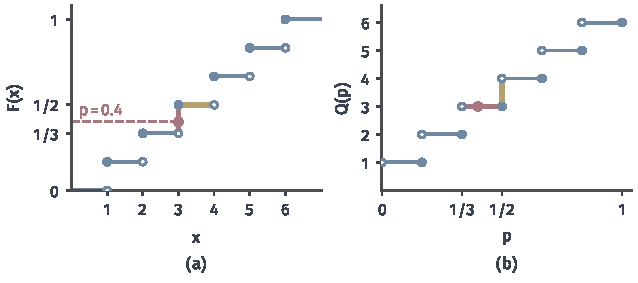
\includegraphics[width=108mm]{figures/07-probability/01-elementary-probability/matplotlib/rvd-quantile-dice/figure.pdf}
  \caption{公平骰子的分布函数与分位数函数。(a)分布函数，红色竖线是$x=3$处从$1/3$到$1/2$的跳跃，红色虚线$p=0.4$落在跳跃之内；黄线是高度$1/2$的平台$[3,4)$。(b)分位数函数，跳跃变成$(1/3,1/2]$上的平台（红线），红点是$Q(0.4)=3$；平台变成$p=1/2$处从$3$到$4$的跳跃（黄线）。实心点在每段右端，表示$Q$在跳跃点取左侧的值。}
  \label{fig:rvd-quantile-dice}
\end{BookInlineFigure}

图中可以看出两者的对偶。分布函数在$x=3$处跳跃$1/6$，累计概率在$(1/3,1/2]$中的所有$p$都“首次达到”于同一个位置$3$，于是分位数函数在这一段上是平台。分布函数在$[3,4)$上是平台，说明这一段没有质量，$p$稍大于$1/2$时阈值必须越过整段平台才能累计到更多概率，于是分位数函数在$p=1/2$处跳跃。几何上，分位数函数的图像就是把分布函数的图像沿对角线翻转，再在跳跃处按约定取左侧的值。

分位数函数单调不减，这由式~\eqref{eq:rvd-quantile}中集合$A_p$随$p$增大而缩小得到。它还是左连续的：设$p_n\uparrow p$，则$Q(p_n)$单调不减且不超过$Q(p)$，有极限$L\leq Q(p)$。对每个$n$有$Q(p_n)\leq L$，由引理$p_n\leq F(L)$；令$n\to\infty$得$p\leq F(L)$，再由引理$Q(p)\leq L$。所以$L=Q(p)$。分布函数右连续，分位数函数左连续，这是同一个约定的两面。

表~\ref{tab:rvd-cdf-vs-quantile}把两个函数的对应关系列在一起。

\begin{BookInlineTable}
  \centering
  \begin{tabular}{lll}
    \toprule
    & 分布函数$F$ & 分位数函数$Q$\\
    \midrule
    输入与输出 & 阈值$x\mapsto$累计概率 & 累计概率$p\mapsto$阈值\\
    定义域 & 全体实数 & $(0,1)$\\
    连续性约定 & 右连续 & 左连续\\
    跳跃 & 单点上的质量 & 一段没有质量的区间\\
    平台 & 一段没有质量的区间 & 单点上的质量\\
    \bottomrule
  \end{tabular}
  \caption{分布函数与分位数函数的对应。二者由式~\eqref{eq:rvd-quantile-galois}联系，一方的跳跃对应另一方的平台。}
  \label{tab:rvd-cdf-vs-quantile}
\end{BookInlineTable}

\paragraph{几个模型的分位数}
抽检次品数的分布函数是式~\eqref{eq:rvd-inspection-cdf}。用同样的方法读出
\[
  Q(p)=\begin{cases}0,&0<p\leq0.3,\\1,&0.3<p\leq0.9,\\2,&0.9<p<1.\end{cases}
\]
中位数是$1$：不超过$1$件次品的概率是$0.9$，严格少于$1$件的概率是$0.3$，两者把$1/2$夹在中间，与式~\eqref{eq:rvd-quantile-sandwich}一致。

等待时间的分位数函数是$Q(p)=-\ln(1-p)$。中位数和两个四分位数分别是
\[
  Q(\tfrac12)=\ln2\approx0.693,\quad Q(\tfrac14)=\ln\tfrac43\approx0.288,\quad Q(\tfrac34)=\ln4\approx1.386 .
\]
半数顾客等待不到$0.7$分钟，中间一半顾客的等待落在约$0.29$到$1.39$分钟之间。两个四分位数之差$Q(3/4)-Q(1/4)$称为\term{四分位距}（interquartile range），这里等于$\ln3\approx1.099$分钟，它从位置的角度衡量取值的分散程度。

另两个模型的分位数也有直接的含义。圆盘中随机点到圆心的距离满足$F_R(r)=r^{2}$，解得$Q(p)=\sqrt{p}$，中位数$\sqrt{1/2}\approx0.707$：一半的点落在半径约$0.707$的圆之外，因为这个圆的面积恰是整个圆盘的一半。

首次掷出六点所需的次数$N$满足$F_N(k)=1-(5/6)^{k}$。由式~\eqref{eq:rvd-quantile-galois}，$Q(p)\leq k$当且仅当$(5/6)^{k}\leq1-p$，即$k\geq\ln(1-p)/\ln(5/6)$，所以$Q(p)$是不小于$\ln(1-p)/\ln(5/6)$的最小正整数。算两个值：
\[
  F_N(3)=1-\tfrac{125}{216}\approx0.4213,\qquad F_N(4)=1-\tfrac{625}{1296}\approx0.5177 .
\]
累计概率在$k=4$时首次超过$1/2$，中位数是$4$。取$p=0.9$，$\ln0.1/\ln(5/6)\approx12.63$，于是$Q(0.9)=13$：要有九成把握见到六点，得准备掷$13$次。

\paragraph{平台上的中位数}
平台意味着一段没有质量的区间。设某服务只在两个时段开放，到达时刻$X$（单位：小时）在$[0,1]$与$[2,3]$上各以一半的概率均匀分布，即密度在这两段上为$1/2$，其余处为$0$。由式~\eqref{eq:rvd-cdf-from-density}，
\[
  F(x)=\begin{cases}x/2,&0\leq x\leq1,\\1/2,&1\leq x\leq2,\\(x-1)/2,&2\leq x\leq3,\end{cases}
\]
$x<0$时为$0$，$x>3$时为$1$。

图~\ref{fig:rvd-quantile-gap}显示，$F$在$[1,2]$上停在$1/2$。这一段的每个$m$都满足$\mathbb{P}(X\leq m)\geq1/2$且$\mathbb{P}(X\geq m)\geq1/2$，都把质量分成相等的两半。式~\eqref{eq:rvd-quantile}取其中最左的一个，$Q(1/2)=1$。也有书取平台的中点$1.5$，约定不同，但只有$F$在高度$p$处有平台时才会出现这种差别。

\begin{BookInlineFigure}
  \centering
  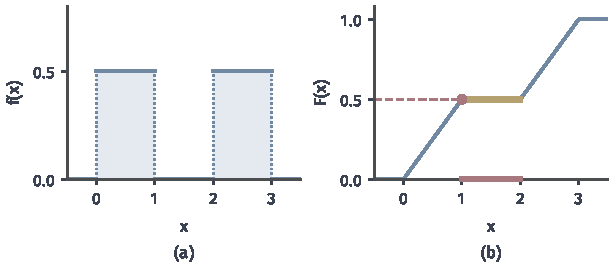
\includegraphics[width=104mm]{figures/07-probability/01-elementary-probability/matplotlib/rvd-quantile-gap/figure.pdf}
  \caption{密度有空档时的中位数。(a)密度在$[0,1]$与$[2,3]$上为$1/2$，中间为$0$；(b)分布函数在$[1,2]$上是高度$1/2$的平台（黄线），横轴上的红线$[1,2]$中每一点都把质量平分，红点是约定的中位数$Q(1/2)=1$。}
  \label{fig:rvd-quantile-gap}
\end{BookInlineFigure}

\paragraph{用二分法求分位数}
分布函数没有显式的反函数时，分位数要用数值方法求。引理~\ref{lem:rvd-quantile-galois}给出一个只用单调性的办法：对任意试探点$m$，计算$F(m)$并与$p$比较，$F(m)\geq p$说明$Q(p)\leq m$，否则$Q(p)>m$。每比较一次，就能把包含$Q(p)$的区间砍掉一半。这一判断不要求$F$连续或严格递增，跳跃和平台都不影响它。

以第~\ref{sec:rvd-mass-density}节的密度$6x(1-x)$为例，$F(x)=3x^{2}-2x^{3}$（$0\leq x\leq1$），求$0.9$分位数。中位数由对称性等于$1/2$，$0.9$分位数则要解三次方程$3x^{2}-2x^{3}=0.9$。从$[0,1]$出发，它一定包含$Q(0.9)$。每一轮取当前区间的中点$m$：若$F(m)\geq0.9$，把右端换成$m$；否则把左端换成$m$。前八轮的结果列在表~\ref{tab:rvd-bisection}中。

\begin{BookInlineTable}
  \centering
  \begin{tabular}{rllll}
    \toprule
    轮次 & 当前区间 & 中点$m$ & $F(m)$ & 判断\\
    \midrule
    1 & $[0,1]$ & $0.5$ & $0.5$ & $<0.9$，取右半\\
    2 & $[0.5,1]$ & $0.75$ & $0.8438$ & $<0.9$，取右半\\
    3 & $[0.75,1]$ & $0.875$ & $0.9570$ & $\geq0.9$，取左半\\
    4 & $[0.75,0.875]$ & $0.8125$ & $0.9077$ & $\geq0.9$，取左半\\
    5 & $[0.75,0.8125]$ & $0.78125$ & $0.8774$ & $<0.9$，取右半\\
    6 & $[0.78125,0.8125]$ & $0.796875$ & $0.8930$ & $<0.9$，取右半\\
    7 & $[0.796875,0.8125]$ & $0.8046875$ & $0.9005$ & $\geq0.9$，取左半\\
    8 & $[0.796875,0.8046875]$ & $0.80078125$ & $0.8967$ & $<0.9$，取右半\\
    \bottomrule
  \end{tabular}
  \caption{用二分法求$F(x)=3x^{2}-2x^{3}$的$0.9$分位数。每一轮区间长度减半，八轮后区间为$[0.80078125,0.8046875]$，长度$2^{-8}$。}
  \label{tab:rvd-bisection}
\end{BookInlineTable}

八轮之后，$Q(0.9)$被夹在$[0.80078,0.80469]$中，长度$2^{-8}\approx0.0039$。继续下去，区间收缩到$Q(0.9)\approx0.8042$。$k$轮之后区间长度是初始长度乘以$2^{-k}$，要达到精度$\varepsilon$只需约$\log_2(1/\varepsilon)$轮，每轮计算一次$F$。初始区间若未知，可以先向两侧加倍试探，直到找到$F(a)<p\leq F(b)$的两点。

\paragraph{分位数函数确定分布}
分位数函数是分布函数的广义逆，它是否也记下了全部信息？答案是肯定的，而且可以直接从引理~\ref{lem:rvd-quantile-galois}读出。对每个$x$，满足$Q(p)\leq x$的$p$恰是$(0,1)$中不超过$F(x)$的那些数，于是在$0<F(x)<1$时
\[
  F(x)=\max\{p\in(0,1):Q(p)\leq x\}.
\]
$F(x)=0$或$1$时，这个集合分别是空集或整个$(0,1)$，同样能读出$F(x)$。所以两个分布的分位数函数相同，它们的分布函数就相同。

还可以用分位数函数把一个最简单的随机变量变成任意给定分布的随机变量。设$U$有密度$1$（$0<u<1$），其余处为$0$，则$\mathbb{P}(U\leq u)=u$（$0\leq u\leq1$）。

\begin{theorem}[分位数变换]
\label{thm:rvd-quantile-transform}
设$F$是一个分布函数，$Q$是它的分位数函数，$U$如上。则$Q(U)$的分布函数是$F$。
\end{theorem}

\begin{proof}
$U$以概率$1$落在$(0,1)$中，那里$Q$有定义。对任意$x$，由引理~\ref{lem:rvd-quantile-galois}，$Q(U)\leq x$与$U\leq F(x)$是同一个事件，所以
\[
  \mathbb{P}(Q(U)\leq x)=\mathbb{P}(U\leq F(x))=F(x),
\]
最后一步用到$0\leq F(x)\leq1$。
\end{proof}

这个定理把“沿实轴均匀铺开的单位质量”按分位数函数重新安放：$U$落在$(1/3,1/2]$中的那一份质量，在骰子的例子中全部被送到$3$，于是$3$分到$1/6$的概率。

\paragraph{分位数与尾概率}
给定阈值$x$，事件$\{X>x\}$的概率$1-F(x)$称为$x$处的尾概率，它描述质量在$x$右侧的残余。给定小的比例$\alpha$，上侧分位数$Q(1-\alpha)$是“超过它的概率至多为$\alpha$”的最小阈值：由式~\eqref{eq:rvd-quantile-sandwich}，
\[
  \mathbb{P}\bigl(X>Q(1-\alpha)\bigr)=1-F\bigl(Q(1-\alpha)\bigr)\leq\alpha .
\]
尾概率和分位数是从两个方向读同一条曲线：前者由横轴读纵轴，后者由纵轴读横轴。

图~\ref{fig:rvd-quantile-tail}用等待时间演示。(a)从纵轴上的$0.5$和$0.9$出发读出中位数$\ln2$和$0.9$分位数$\ln10$。(b)画的是尾概率$1-F_T(t)=\mathrm{e}^{-t}$：从$t=1$读出$\mathbb{P}(T>1)=\mathrm{e}^{-1}\approx0.368$；在$t=\ln10$处尾概率恰为$0.1$，浅蓝面积就是这剩下的一成顾客。完整的分布已知时，两个方向都能精确计算；只知道分布的少数数值特征时，第~\ref{chap:tail-probabilities}章研究怎样给尾概率一个上界。

\begin{BookInlineFigure}
  \centering
  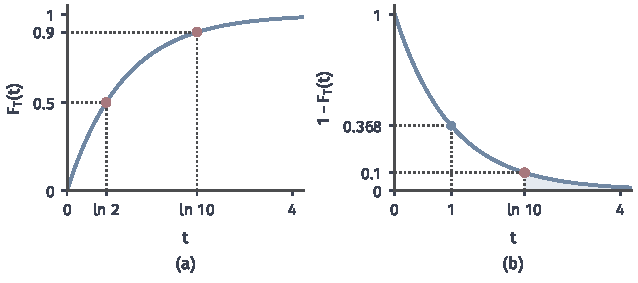
\includegraphics[width=108mm]{figures/07-probability/01-elementary-probability/matplotlib/rvd-quantile-tail/figure.pdf}
  \caption{等待时间的分位数与尾概率。(a)分布函数$1-\mathrm{e}^{-t}$，红点给出$Q(0.5)=\ln2$与$Q(0.9)=\ln10$；(b)尾概率$\mathrm{e}^{-t}$，蓝点是$t=1$处的$0.368$，红点是$t=\ln10$处的$0.1$，浅蓝区域表示超过$0.9$分位数的那部分。}
  \label{fig:rvd-quantile-tail}
\end{BookInlineFigure}

\paragraph{改变单位}
把等待时间从分钟换成秒，所有分位数都乘以$60$，这对一般的平移和正比例缩放都成立。设$a>0$，$b$为实数，$Y=aX+b$。对任意$y$，$\{Y\leq y\}=\{X\leq(y-b)/a\}$，所以$F_Y(y)=F_X((y-b)/a)$。由引理~\ref{lem:rvd-quantile-galois}，
\[
  Q_Y(p)\leq y\iff p\leq F_X\Bigl(\frac{y-b}{a}\Bigr)\iff Q_X(p)\leq\frac{y-b}{a}\iff aQ_X(p)+b\leq y .
\]
对一切$y$成立，于是$Q_Y(p)=aQ_X(p)+b$。$a<0$时不等号方向翻转，下侧分位数变成上侧，平台和跳跃处的约定也随之改变，需要另行处理。

\paragraph{描述位置而不是平均}
中位数和其他分位数描述的是分布的位置：取值在什么地方把质量按给定比例分开。它们只依赖取值的先后顺序和累计质量，不依赖远处的取值究竟有多远。

设$X$以概率$1/5$取$1,2,3,4,5$，中位数是$3$。把最大的取值$5$改成$12$，其余不变，$F$在$3$及其左侧不受影响，中位数仍是$3$。另一种描述中心的方式是按概率加权求和$\sum_xx\,p_X(x)$，下一章把它作为期望来研究。它同时看取值的大小，改动后从
\[
  \tfrac15(1+2+3+4+5)=3
\]
变为
\[
  \tfrac15(1+2+3+4+12)=4.4 .
\]
图~\ref{fig:rvd-median-shift}画出了这一对比：一个远处的取值就能把加权和拉过去，中位数却纹丝不动。

\begin{BookInlineFigure}
  \centering
  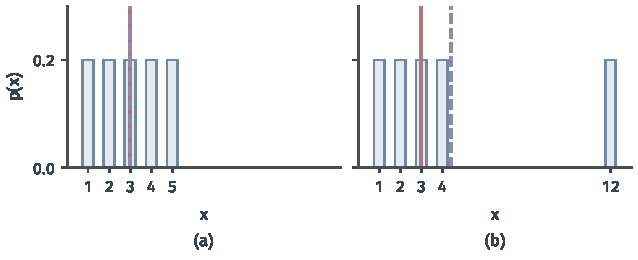
\includegraphics[width=108mm]{figures/07-probability/01-elementary-probability/matplotlib/rvd-median-shift/figure.pdf}
  \caption{中位数只看顺序。每个取值的概率都是$1/5$，红线是中位数$3$，紫色虚线是加权和$\sum_xx\,p_X(x)$。(a)取值$1,\dots,5$，两者都等于$3$；(b)把$5$移到$12$，中位数不变，加权和变为$4.4$。}
  \label{fig:rvd-median-shift}
\end{BookInlineFigure}

分位数还有一个优点：它对每个分布都存在。上一节的概率表$p_X(k)=1/(k(k+1))$有$F_X(1)=1/2$，所以中位数是$1$；而加权和
\[
  \sum_{k=1}^{\infty}k\cdot\frac{1}{k(k+1)}=\sum_{k=1}^{\infty}\frac{1}{k+1}
\]
是发散的调和级数，没有有限值。尾部质量衰减太慢时，加权平均会失去意义，分位数照样可以计算。至于什么时候加权平均存在、它与分位数各回答什么问题，在第~\ref{chap:random-variable-moments}章讨论。


\section{分布表示的边界}
\label{sec:rvd-representation-limits}

到目前为止，每个例子要么能列成一张概率表，要么有密度。是不是所有随机变量都属于这两类之一？先看一个很平常的等待问题，它两类都不属于。

\paragraph{有时不用等}
顾客来到窗口时，若窗口恰好空闲（概率$0.3$），等待时间为$0$；否则等待时间按式~\eqref{eq:rvd-waiting-cdf}的规律分布。记等待时间为$W$。由全概率公式，对$t\geq0$，
\[
  \mathbb{P}(W\leq t)=0.3\cdot1+0.7\,(1-\mathrm{e}^{-t}),
\]
其中第一项是窗口空闲、等待为$0$的情形，第二项是窗口忙、等待不超过$t$的情形。于是
\begin{equation}
  F_W(t)=\begin{cases}0,&t<0,\\0.3+0.7\,(1-\mathrm{e}^{-t}),&t\geq0.\end{cases}
  \label{eq:rvd-mixed-cdf}
\end{equation}
图~\ref{fig:rvd-mixed-cdfs}(a)画出了这条曲线：它在$0$处从$0$跳到$0.3$，之后连续上升。

\begin{BookInlineFigure}
  \centering
  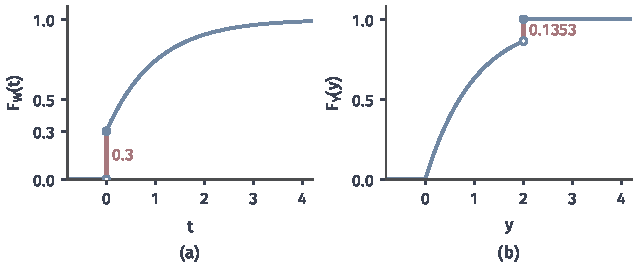
\includegraphics[width=108mm]{figures/07-probability/01-elementary-probability/matplotlib/rvd-mixed-cdfs/figure.pdf}
  \caption{既有跳跃又有连续上升的分布函数。(a)可能不用等的等待时间$W$，在$0$处跳跃$0.3$（红线），之后按$0.7(1-\mathrm{e}^{-t})$连续增加；(b)截断的等待时间$Y=\min\{T,2\}$，在$[0,2)$上与$1-\mathrm{e}^{-y}$相同，在$2$处跳跃$\mathrm{e}^{-2}\approx0.1353$。空心点是左极限，实心点是函数值。}
  \label{fig:rvd-mixed-cdfs}
\end{BookInlineFigure}

$W$不是离散随机变量。按模型，$0$这一点带有概率$0.3$；分布函数在其余各点连续，用第~\ref{sec:rvd-mass-density}节对等待时间所用的夹逼，其余每一点的概率都是$0$；可数个点上的质量加起来至多$0.3$，凑不满$1$。$W$也没有密度。若有密度，定理~\ref{thm:rvd-density-cdf}要求$\mathbb{P}(W=0)=0$，与$0.3$矛盾。概率表和密度都只能描述$W$的一部分质量。

计算时把两部分分开处理：跳跃部分求和，连续部分积分。对区间$B$，
\begin{equation}
  \mathbb{P}(W\in B)=0.3\cdot\mathbf{1}_{B}(0)+0.7\int_{B\cap(0,\infty)}\mathrm{e}^{-t}\,\mathrm{d}t,
  \label{eq:rvd-mixed-prob}
\end{equation}
其中$\mathbf{1}_{B}(0)$在$0\in B$时为$1$，否则为$0$。下面用三个区间演示。是否包含$0$决定了第一项：
\[
  \mathbb{P}(W\leq1)=0.3+0.7(1-\mathrm{e}^{-1})\approx0.7425,
\]
\[
  \mathbb{P}(0<W\leq1)=0.7(1-\mathrm{e}^{-1})\approx0.4425 .
\]
远离$0$的区间只有第二项，例如$\mathbb{P}(W>2)=0.7\,\mathrm{e}^{-2}\approx0.0947$。

分位数照样按式~\eqref{eq:rvd-quantile}计算。$p\leq0.3$时，$F_W(0)=0.3\geq p$而$t<0$时$F_W(t)=0$，所以$Q(p)=0$：有三成顾客根本不用等。$p>0.3$时解$0.3+0.7(1-\mathrm{e}^{-t})=p$，得
\[
  Q(p)=\ln\frac{0.7}{1-p},\qquad 0.3<p<1 .
\]
中位数是$\ln(7/5)\approx0.336$分钟，比不考虑空闲时的$\ln2\approx0.693$分钟短。

\paragraph{截断产生的跳跃}
这类分布并不罕见，对有密度的变量取函数就可能产生。设顾客最多等$2$分钟，等不到就离开，记录到的时长是$Y=\min\{T,2\}$。$y<2$时$\{Y\leq y\}=\{T\leq y\}$；$y\geq2$时$Y\leq y$总成立。所以
\[
  F_Y(y)=\begin{cases}0,&y<0,\\1-\mathrm{e}^{-y},&0\leq y<2,\\1,&y\geq2.\end{cases}
\]
它在$2$处跳跃，跳跃高度$\mathrm{e}^{-2}\approx0.1353$就是$\mathbb{P}(T\geq2)$：所有等待超过$2$分钟的质量都被堆到了$2$这一点上（图~\ref{fig:rvd-mixed-cdfs}(b)）。测量仪器有量程上限、记录有截止时间时，都会出现这种情形。

$Y$的分位数显示出跳跃的另一面。$p\leq1-\mathrm{e}^{-2}\approx0.8647$时，方程$1-\mathrm{e}^{-y}=p$在$[0,2)$中有解，$Q_Y(p)=-\ln(1-p)$，与$T$的分位数相同；$p>0.8647$时，累计概率在$y=2$处才首次达到$p$，$Q_Y(p)=2$。分布函数在$2$处的跳跃，变成了分位数函数在$(0.8647,1)$上的平台。截断只改变了高分位数，中位数仍是$\ln2$。

\paragraph{分离跳跃}
两个例子都由“跳跃部分”和“连续部分”组成。这种分离对任何分布函数都可以做到：先证明跳跃只能有可数个，再把它们集中成一张概率表，剩下的部分连续。

\begin{theorem}[分布函数的跳跃分解]
\label{thm:rvd-jump-decomposition}
设$F$单调不减、右连续，且$\lim_{x\to-\infty}F(x)=0$，$\lim_{x\to+\infty}F(x)=1$。记$J(a)=F(a)-F(a^{-})$为$a$处的跳跃高度。则
\begin{enumerate}
  \item 跳跃点$\{a:J(a)>0\}$至多可数，且跳跃高度的总和不超过$1$；
  \item 令
  \begin{equation}
    F_{\mathrm{d}}(x)=\sum_{a\leq x}J(a),\qquad F_{\mathrm{c}}(x)=F(x)-F_{\mathrm{d}}(x),
    \label{eq:rvd-jump-parts}
  \end{equation}
  则$F_{\mathrm{c}}$单调不减且处处连续。
\end{enumerate}
\end{theorem}

\begin{proof}
先看有限个跳跃点$a_1<a_2<\dots<a_m$。对相邻的两点，单调性给出$F(a_k)\leq F(a_{k+1}^{-})$，所以各段增量
\[
  F(a_m)-F(a_1^{-})=\sum_{k=1}^{m}J(a_k)+\sum_{k=1}^{m-1}\bigl(F(a_{k+1}^{-})-F(a_k)\bigr)\geq\sum_{k=1}^{m}J(a_k).
\]
左边不超过$1$，所以任意有限个跳跃高度之和不超过$1$。

固定正整数$n$。若有$m$个点的跳跃高度都大于$1/n$，则$m/n<1$，即$m<n$。所以跳跃高度大于$1/n$的点少于$n$个。全部跳跃点是这些有限集对$n=1,2,\dots$的并，因而至多可数；任意有限部分和不超过$1$，总和也不超过$1$。

再看$F_{\mathrm{c}}$。对$x<y$，把上面的论证用在$(x,y]$中有限个跳跃点上，再取上确界，得到
\[
  F(y)-F(x)\geq\sum_{x<a\leq y}J(a)=F_{\mathrm{d}}(y)-F_{\mathrm{d}}(x),
\]
即$F_{\mathrm{c}}(y)\geq F_{\mathrm{c}}(x)$。

$F_{\mathrm{d}}$与离散变量的分布函数结构相同：可数个点$a$各带非负质量$J(a)$，只是总量可能小于$1$。定理~\ref{thm:rvd-cdf-properties}中右连续与左极限的证明只用到质量非负、总和有限，所以$F_{\mathrm{d}}$右连续，并且在$a$处的跳跃恰为$J(a)$。$F$本身右连续、在$a$处跳跃$J(a)$，二者相减，$F_{\mathrm{c}}$右连续且在每点的跳跃为$0$，即处处连续。
\end{proof}

对$W$，$F_{\mathrm{d}}(t)=0.3\cdot\mathbf{1}_{\{t\geq0\}}$，连续部分在$t\geq0$时为$0.7(1-\mathrm{e}^{-t})$，它有密度$0.7\,\mathrm{e}^{-t}$，式~\eqref{eq:rvd-mixed-prob}正是按这一分解写成的。对$Y$，跳跃部分是$2$处的$\mathrm{e}^{-2}$，连续部分在$[0,2]$上由密度$\mathrm{e}^{-y}$积分得到。那么，连续部分是不是总有密度？

\paragraph{分布函数连续也未必有密度}
下面构造一个分布函数处处连续、却没有密度的随机变量。反复抛一枚公平硬币，各次独立，第$k$次正面记$D_k=1$，反面记$D_k=0$。令
\begin{equation}
  X=\sum_{k=1}^{\infty}\frac{2D_k}{3^{k}} .
  \label{eq:rvd-cantor}
\end{equation}
级数各项不超过$2/3^{k}$，总是收敛，$X\in[0,1]$。用三进制看，$X$的第$k$位小数是$2D_k$，只取$0$或$2$，永远不取$1$。

前$n$次抛掷决定了$X$落在哪一段。前$n$项的和是若干个$2/3^{k}$之和，剩余各项之和满足
\[
  0\leq\sum_{k>n}\frac{2D_k}{3^{k}}\leq\sum_{k>n}\frac{2}{3^{k}}=\frac{1}{3^{n}},
\]
所以$X$落在以前$n$项之和为左端点、长$3^{-n}$的闭区间里。前$n$次抛掷有$2^{n}$种等可能的结果，对应$2^{n}$个这样的区间，每个的概率是$2^{-n}$。

这些区间可以一层层画出来（图~\ref{fig:rvd-cantor-split}）。第一层是$[0,1/3]$和$[2/3,1]$，由$D_1=0$或$1$决定，各得一半质量；中间的$(1/3,2/3)$对应三进制首位为$1$，得不到任何质量。下一层把每个保留的区间再三等分，质量对半分给左右两段，中间一段又是空的。记第$n$层的$2^{n}$个区间之并为$C_n$，则$\mathbb{P}(X\in C_n)=1$，而$C_n$的总长度是$(2/3)^{n}$。

\begin{BookInlineFigure}
  \centering
  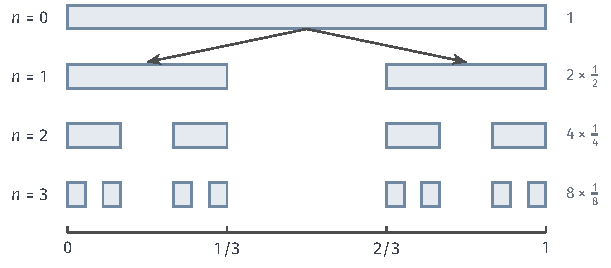
\includegraphics[width=104mm]{figures/07-probability/01-elementary-probability/tikz/rvd-cantor-split/figure.pdf}
  \caption{式~\eqref{eq:rvd-cantor}中$X$的质量怎样一层层分配。第$n$层有$2^{n}$个长$3^{-n}$的区间，每个区间的质量平分给它的左右两个三分之一，中间三分之一得不到质量。右侧是每层区间的个数与各自的质量；第$n$层总长$(2/3)^{n}$，总质量始终为$1$。}
  \label{fig:rvd-cantor-split}
\end{BookInlineFigure}

第一个结论：$F_X$处处连续。同一层的区间彼此之间至少隔着长$3^{-n}$的空档，所以长度小于$3^{-n}$的任何区间至多与该层的两个区间相交。对任意$x$和$0<h<3^{-n}/2$，区间$(x-h,x+h]$长度小于$3^{-n}$，于是
\[
  F_X(x+h)-F_X(x-h)=\mathbb{P}(x-h<X\leq x+h)\leq2\cdot2^{-n}.
\]
$n$可以任意大，所以$h\to0$时这个差趋于$0$，$F_X$在$x$处连续。特别地，每个单点的概率都是$0$，$X$不是离散随机变量。

第二个结论：$X$没有有界的密度。若$X$有密度$f$且$f\leq K$，则$X$落在$C_n$的概率是$f$在这$2^{n}$个区间上的积分之和，不超过$K$乘总长度：
\[
  1=\mathbb{P}(X\in C_n)\leq K\Bigl(\frac23\Bigr)^{n}.
\]
令$n\to\infty$，右边趋于$0$，矛盾。直观地说，全部质量挤在总长度任意小的集合上，单位长度上的概率只能无限大。

去掉“有界”这个限制，结论仍然成立：$X$根本没有密度。对无界的被积函数，上面的估计不再可用，严格证明需要比黎曼积分更一般的积分理论，可参考\BookChapterRef{chap:measure-densities}{卷四第8章“测度的密度”}。从分布函数一侧也能看到问题所在：$F_X$在被删去的每个中间三分之一上都是常数（那里没有质量），这些开区间的总长度是$1-(2/3)^{n}\to1$，所以$F_X$的导数在总长为$1$的范围内都是$0$；然而$F_X$从$0$升到了$1$。对导数积分只会得到$0$。定理~\ref{thm:rvd-cdf-to-density}的途径在这里失效，因为它要求除有限个点外可导。而对每一层都被保留的点$x$，包含$x$的第$n$层区间长$3^{-n}$，$F_X$在其上增加$2^{-n}$，差商为$(3/2)^{n}$，随$n$增大趋于无穷，所以$F_X$在这些点处不可导，这样的点有无穷多个。

图~\ref{fig:rvd-cantor-cdf}画出了$F_X$，它称为Cantor函数，$X$的分布称为\term{Cantor分布}（Cantor distribution）。黄线和紫线是把第$1$、$2$层的质量在各区间内均匀铺开得到的分布函数，蓝线是极限。每加细一层，上升的部分被压缩到更短的区间里，坡度变陡，平台变多。

\begin{BookInlineFigure}
  \centering
  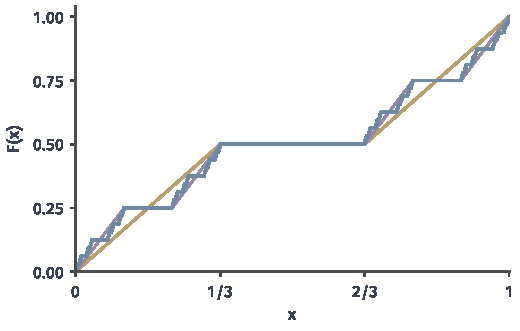
\includegraphics[width=88mm]{figures/07-probability/01-elementary-probability/matplotlib/rvd-cantor-cdf/figure.pdf}
  \caption{Cantor分布的分布函数（蓝线）。黄线与紫线分别把第$1$层、第$2$层区间上的质量均匀铺开，坡度为$(3/2)^{n}$。极限曲线连续，从$0$升到$1$，却在总长为$1$的一组区间上保持水平。}
  \label{fig:rvd-cantor-cdf}
\end{BookInlineFigure}

这个例子是专门构造出来的，在建模中很少直接出现。它说明的是一条边界：离散分布、有密度的分布以及二者的组合，并没有穷尽全部分布。一般的分布函数在去掉跳跃部分之后，连续部分还可以再分成有密度的部分和像Cantor函数这样没有密度的部分，相应的分解定理在卷四的同一章中给出。

\paragraph{各种表示的适用范围}
图~\ref{fig:rvd-representations}把本章的例子放到一起。分布函数对所有分布都存在；概率表只适用于离散分布；密度只适用于有密度的分布；像$W$和$Y$那样的分布需要两者组合；Cantor分布的分布函数连续，却两者都用不上。

\begin{BookInlineFigure}
  \centering
  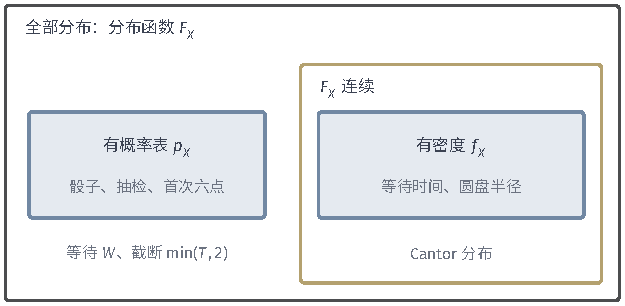
\includegraphics[width=105mm]{figures/07-probability/01-elementary-probability/tikz/rvd-representations/figure.pdf}
  \caption{各种表示的适用范围。外框是全部分布，它们都有分布函数；左侧蓝框是有概率表的离散分布，右侧黄框是分布函数连续的分布，其中蓝框是有密度的分布。框外标注的是两者都不适用的例子：可能不用等的$W$与截断的$\min\{T,2\}$既有跳跃又有连续部分，Cantor分布连续却没有密度。}
  \label{fig:rvd-representations}
\end{BookInlineFigure}

要对所有这些情形使用同一种语言，就不能再依赖“求和”与“黎曼积分”这两种具体的计算方式，而要直接把分布看作对实轴子集赋予概率的规则，并为它建立统一的积分。第~\ref{chap:probability-spaces}章完成这件事：概率表、密度以及它们的组合都成为同一种对象的特例，Cantor分布也能放进同一框架。在那之前，本部分只使用离散模型、密度模型以及按式~\eqref{eq:rvd-mixed-prob}那样分开计算的组合。


\section{本章小结}
\label{sec:rvd-summary}

本章从“由试验结果算出的数”出发。随机变量是样本空间上的函数，它把结果上的概率搬到实轴上，得到分布。分布只记录取值落在各处的概率，不记录这些取值来自哪个结果，所以同分布的变量可以在每次试验中取值完全不同，涉及几个变量之间关系的问题要留给随机向量。

分布有几种表示，各有成立的条件。分布函数$F_X(x)=\mathbb{P}(X\leq x)$对一切随机变量都有定义，单调不减、右连续、两端趋于$0$和$1$，跳跃高度是单点概率。概率质量函数只适用于离散变量，用求和计算概率；密度只适用于有密度的变量，用积分计算概率，它的值是单位长度上的概率，可以大于$1$，在有限个点处改动不影响分布。分位数$Q(p)=\inf\{x:F(x)\geq p\}$从反方向读分布函数，对一切分布都存在，并且与分布函数相互确定。

用可能不用等的等待时间$W$把这些表示串起来，可以看清各种表示分别用在哪里。分布函数由式~\eqref{eq:rvd-mixed-cdf}给出，任何区间的概率都能从它和它的左极限读出，例如$\mathbb{P}(W\leq1)\approx0.7425$。$W$在$0$处有$0.3$的质量，这部分只能用概率表描述；其余$0.7$的质量有密度$0.7\,\mathrm{e}^{-t}$，只能用积分描述；两者都不能单独代表整个分布。分位数在$p\leq0.3$时为$0$，中位数是$\ln(7/5)\approx0.336$分钟，它们描述的是质量按比例分开的位置。

表~\ref{tab:rvd-summary}汇总了各种表示。选用哪一种，先看分布属于哪一类，再看问题是给定范围求概率，还是给定概率求阈值。

\begin{BookInlineTable}
  \centering
  \begin{tabular}{lll}
    \toprule
    表示 & 适用范围 & 计算方式\\
    \midrule
    分布函数$F_X$ & 一切分布 & 相减，端点处用左极限\\
    质量函数$p_X$ & 离散分布 & 对取值求和\\
    密度$f_X$ & 有密度的分布 & 在区间上积分\\
    跳跃与密度组合 & 如$W$、$\min\{T,2\}$ & 跳跃求和，连续部分积分\\
    分位数$Q$ & 一切分布 & 给定概率反求阈值\\
    \bottomrule
  \end{tabular}
  \caption{分布的几种表示及其适用范围。Cantor分布的分布函数连续，却既无概率表也无密度，只能用分布函数或分位数函数描述。}
  \label{tab:rvd-summary}
\end{BookInlineTable}

这些表示的边界也要记住。分布函数连续不保证密度存在；一般情形下哪些集合可以赋予概率、分布函数为什么唯一确定分布，都在第~\ref{chap:probability-spaces}章统一建立。完整的分布包含全部概率规律，但使用起来往往太细。下一章从分布中提取平均位置和波动大小这样的少数数值，并说明它们存在的条件；中位数与加权平均的对比已经表明，几个数值只是分布的概括，不能代替分布本身。


\chapter{随机变量的数值特征}
\label{chap:random-variable-moments}

掷一枚均匀的骰子：点数是$1$、$2$、$3$时没有奖金，点数是$4$或$5$时得$3$元，点数是$6$时得$6$元。奖金$X$的分布是一张三行的概率表，它回答了每种结果的机会有多大。可是参与之前，人们更想先知道两个数：平均能拿多少钱，以及每次的结果会离这个平均有多远。如果参加一次要付$2.5$元，值不值？另一个游戏平均奖金相同，但输赢更集中，又该怎样比较？

把一整张概率表压缩成少数几个数，会马上遇到三类问题。第一，平均要怎样定义，才能同时处理有限个取值、可数个取值和密度？取值可以无穷多时，加权和可能发散，甚至随求和次序改变。第二，平均满足哪些运算规则，算一个函数的平均时是否必须先求出这个函数的分布？第三，除了平均位置和波动尺度，还有哪些数能描述分布的偏斜与尾部，这些数在什么条件下存在，又能在多大程度上代替分布本身？

本章用上面的奖金表和$(0,1)$上的密度$f_X(x)=2x$作为贯穿全章的两个例子。先定义期望，讲清它的存在条件、运算性质、函数的期望和凸函数的期望；再用期望定义方差，研究计算方法、平移缩放规律和标准化；最后把幂次推广到一般的阶，讨论矩的存在性、计算、偏度与峰度，并说明有限个矩为何不能确定分布。分位数已在第~\ref{chap:random-variables}章定义，这里只在比较均值与中位数时用到它。

\section{期望}
\label{sec:rvm-expectation}

骰子游戏平均能拿多少钱？这个问题要求用一个数概括整张概率表，而且这个数应当按概率给各个取值加权。取值只有有限个时，加权平均就是一个有限和；取值有可数无穷个或由密度给出时，有限和变成级数或积分，就必须先检查它是否有意义。本节先给出定义和存在条件，再建立运算规则，然后说明怎样直接计算函数的平均，最后比较“先平均再变换”与“先变换再平均”。

\subsection{定义}
\label{sec:rvm-expectation-definition}

\paragraph{有限个取值}
设想把骰子游戏玩$6000$次。按概率，大约有$3000$次拿到$0$元，$2000$次拿到$3$元，$1000$次拿到$6$元。总奖金约为
\[
 0\times3000+3\times2000+6\times1000=12000,
\]
平均每次约$2$元。把次数换成比例，这个计算就是按概率加权：
\[
 0\times\tfrac12+3\times\tfrac13+6\times\tfrac16=2 .
\]
重复次数越多，实际平均为什么越接近这个加权和，是第~\ref{chap:laws-of-large-numbers}章大数律的内容。这里只把加权和本身作为定义的出发点，它只用到概率表，与任何一次具体的试验结果无关。

另一种看法来自力学。把总质量$1$按概率分配到数轴上：位置$0$放质量$\tfrac12$，位置$3$放$\tfrac13$，位置$6$放$\tfrac16$。在位置$c$处支起数轴，各质量对支点的力矩之和是$\sum_i(x_i-c)p_X(x_i)$，它等于零时数轴平衡。解出的$c$正是加权和$\sum_ix_ip_X(x_i)=2$。所以加权平均就是这组质量的重心，见图~\ref{fig:rvm-balance}(a)。

\begin{BookInlineFigure}
 \centering
 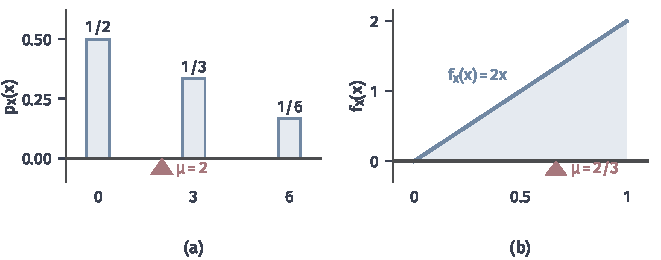
\includegraphics[width=112mm]{figures/07-probability/01-elementary-probability/matplotlib/rvm-balance/figure.pdf}
 \caption{期望是概率质量的重心。(a)奖金表：位置$0,3,6$上分别放质量$\tfrac12,\tfrac13,\tfrac16$（蓝色柱），红色三角是使数轴平衡的支点$\mu=2$，它不是$X$的任何可能取值。(b)密度$f_X(x)=2x$把质量连续地铺在$(0,1)$上，右侧更重，重心在$\mu=2/3$。}
 \label{fig:rvm-balance}
\end{BookInlineFigure}

这个例子说明期望不必是随机变量能取到的值。没有哪一次游戏恰好得$2$元，$2$描述的是质量的平衡位置，而不是某次的典型结果。图中重心偏向左侧，因为一半的质量堆在$0$上；位置$6$虽远，质量却只有$\tfrac16$。

\begin{definition}[有限取值的期望]
\label{def:rvm-expectation-finite}
设随机变量$X$只取有限个值$x_1,\dots,x_n$，概率质量为$p_X(x_i)$。称
\begin{equation}
 \mathbb{E}[X]=\sum_{i=1}^{n}x_i\,p_X(x_i)
 \label{eq:rvm-mean-finite}
\end{equation}
为$X$的\term{期望}（expectation），也称\term{均值}（mean），常记作$\mu$或$\mu_X$。
\end{definition}

\paragraph{从样本点求和}
式~\eqref{eq:rvm-mean-finite}按$X$的取值分组求和。也可以回到试验本身，逐个样本点相加。骰子有六个等可能的点数$\omega=1,\dots,6$，奖金是点数的函数$X(\omega)$。逐点相加得到
\[
 \sum_{\omega=1}^{6}X(\omega)\,\mathbb{P}(\{\omega\})
 =\tfrac16(0+0+0+3+3+6)=2,
\]
与按取值分组的结果相同。图~\ref{fig:rvm-reward-map}显示了这两种算法的关系：先把映到同一个值的样本点归成一组，组内概率之和就是这个值的概率质量。

\begin{BookInlineFigure}
 \centering
 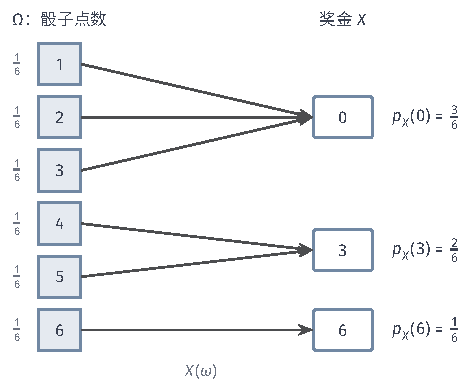
\includegraphics[width=80mm]{figures/07-probability/01-elementary-probability/tikz/rvm-reward-map/figure.pdf}
 \caption{奖金$X$是样本空间$\Omega=\{1,\dots,6\}$上的函数。左侧每个点数的概率是$\tfrac16$；映到同一奖金的点数合成一组，组内概率相加就得到右侧的概率质量。逐点求和与按取值分组求和只是加法的次序不同。}
 \label{fig:rvm-reward-map}
\end{BookInlineFigure}

一般地，若样本空间$\Omega$有限，按$X$的取值把样本点分组，就有
\begin{equation}
 \mathbb{E}[X]=\sum_{\omega\in\Omega}X(\omega)\,\mathbb{P}(\{\omega\}) .
 \label{eq:rvm-mean-sample-points}
\end{equation}
理由是每个样本点恰好落在一组中，而第$i$组的概率之和是$p_X(x_i)$，组内各项的$X(\omega)$都等于$x_i$。有限和可以任意分组与交换次序，所以两种求和结果相同。下一小节将用式~\eqref{eq:rvm-mean-sample-points}证明期望的线性性。

\paragraph{可数个取值}
取值有可数无穷个时，加权和成为级数，这时会出现有限和没有的两个问题：级数可能发散，也可能只在某种求和次序下收敛。先看非负的情形。设$X$取正整数，
\[
 p_X(k)=\frac{1}{k(k+1)},\qquad k=1,2,\dots .
\]
由$\frac{1}{k(k+1)}=\frac1k-\frac1{k+1}$，前$n$项之和是$1-\frac1{n+1}$，它趋于$1$，所以这是一张合法的概率表。

计算加权和时，各项为$k\,p_X(k)=\frac{1}{k+1}$，于是部分和
\[
 \sum_{k=1}^{n}k\,p_X(k)=\sum_{k=1}^{n}\frac{1}{k+1}
\]
随$n$无限增大，增长速度与$\ln n$相同，见图~\ref{fig:rvm-truncated-sums}(a)。各项都非负，部分和单调增加，所以无论按什么次序相加，结果都是$+\infty$。对非负随机变量，这样的结论有明确含义：平均没有上限，我们写$\mathbb{E}[X]=+\infty$。用重心的语言说，质量$\frac{1}{k(k+1)}$随距离$k$衰减得不够快，远处的质量对力矩的贡献加起来没有上界，数轴在任何位置都无法平衡。

有正有负的取值则不同。若正负两部分的加权和都是$+\infty$，部分和的极限取决于正项与负项轮流加入的方式。由级数重排定理，条件收敛的级数重排后可以收敛到任意指定的值，可参考\BookChapterRef{chap:limits-continuity}{卷一第5章“极限与连续”}。概率表里的取值并没有天然的先后次序，所以只有与次序无关的和才适合作为期望。解决办法是把正负两部分分开计算。

\paragraph{正部与负部}
对实数$x$，记$x^{+}=\max\{x,0\}$，$x^{-}=\max\{-x,0\}$，则
\begin{equation}
 x=x^{+}-x^{-},\qquad \lvert x\rvert=x^{+}+x^{-} .
 \label{eq:rvm-pos-neg}
\end{equation}
对随机变量逐个取值使用这两个函数，得到两个非负随机变量$X^{+}$与$X^{-}$，分别称为$X$的\term{正部}（positive part）与\term{负部}（negative part）。$X^{+}$只记录收益，$X^{-}$只记录损失，两者都非负，它们的加权和总有意义，可能是有限数，也可能是$+\infty$。

\paragraph{密度的情形}
有密度时，概率质量连续地铺在数轴上，单位长度上的质量是$f_X(x)$。把小区间$[x,x+\mathrm{d}x]$上的质量$f_X(x)\,\mathrm{d}x$看作放在$x$处，加权和就变成积分。对贯穿例子$f_X(x)=2x$（$0<x<1$），有
\[
 \int_0^1x\cdot2x\,\mathrm{d}x=\left[\tfrac23x^{3}\right]_0^1=\tfrac23 .
\]
图~\ref{fig:rvm-balance}(b)中质量向右堆积，重心落在$2/3$，比区间中点$1/2$偏右。

密度的支撑无界时，积分是反常积分，同样要分正负两部分检查。考虑对称的密度
\[
 f_X(x)=\frac{1}{2x^{2}},\qquad \lvert x\rvert\geq1 .
\]
它在$[1,\infty)$与$(-\infty,-1]$上各有质量$\tfrac12$，总质量为一。正部的积分是
\[
 \int_1^{\infty}x\cdot\frac{1}{2x^{2}}\,\mathrm{d}x=\frac12\int_1^{\infty}\frac{\mathrm{d}x}{x}=+\infty,
\]
负部同理也是$+\infty$。

两侧都无穷时，截断的方式决定了截断后的积分。在$[-a,b]$（$a,b\geq1$）上，正负两侧的贡献分别是$\frac12\ln b$与$-\frac12\ln a$，所以截断积分为$\frac12\ln(b/a)$。对称截断$b=a$得$0$，截断$b=2a$恒得$\frac12\ln2\approx0.35$，截断$b=a^{2}$得$\frac12\ln a\to+\infty$。图~\ref{fig:rvm-truncated-sums}(b)画出了这三种截断。密度关于$0$对称，却不能因此说期望是$0$：期望根本没有定义。

\begin{BookInlineFigure}
 \centering
 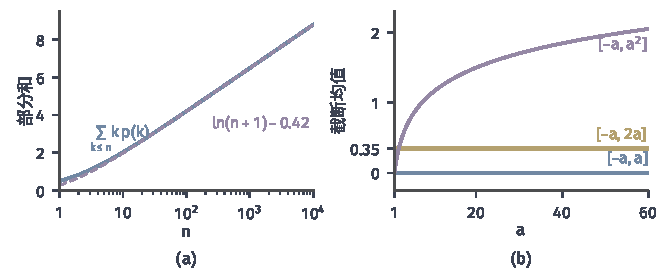
\includegraphics[width=112mm]{figures/07-probability/01-elementary-probability/matplotlib/rvm-truncated-sums/figure.pdf}
 \caption{无穷的加权和。(a)概率表$p_X(k)=1/[k(k+1)]$的部分和$\sum_{k\leq n}k\,p_X(k)$（蓝）与$\ln(n+1)-0.42$（紫色虚线）几乎重合，趋于$+\infty$。(b)对称密度$1/(2x^{2})$（$\lvert x\rvert\geq1$）在$[-a,b]$上的截断积分$\frac12\ln(b/a)$：对称截断（蓝）恒为$0$，$b=2a$（黄）恒为$0.35$，$b=a^{2}$（紫）无界增长。}
 \label{fig:rvm-truncated-sums}
\end{BookInlineFigure}

\paragraph{期望的定义}
上面的例子给出了三种情形：非负变量的加权和总有意义，可能为$+\infty$；有正有负时，只要正负两部分不同时为无穷，差仍有意义；两部分都无穷时没有合理的值。下面的定义同时覆盖概率表与密度。

\begin{definition}[期望]
\label{def:rvm-expectation}
设$X$是取有限或可数个值$x_i$的离散随机变量，概率质量为$p_X$；或$X$有密度$f_X$。$X$的正部与负部的期望定义为
\begin{equation}
 \begin{aligned}
 \mathbb{E}[X^{+}]&=\sum_{x_i>0}x_i\,p_X(x_i)\quad\text{或}\quad\int_0^{\infty}x\,f_X(x)\,\mathrm{d}x,\\
 \mathbb{E}[X^{-}]&=\sum_{x_i<0}(-x_i)\,p_X(x_i)\quad\text{或}\quad\int_{-\infty}^{0}(-x)\,f_X(x)\,\mathrm{d}x,
 \end{aligned}
 \label{eq:rvm-mean-parts}
\end{equation}
它们取值于$[0,+\infty]$。若两者不同时为$+\infty$，定义
\begin{equation}
 \mathbb{E}[X]=\mathbb{E}[X^{+}]-\mathbb{E}[X^{-}] .
 \label{eq:rvm-mean-general}
\end{equation}
若两者都有限，等价地
\begin{equation}
 \mathbb{E}\lvert X\rvert=\mathbb{E}[X^{+}]+\mathbb{E}[X^{-}]<\infty,
 \label{eq:rvm-integrable}
\end{equation}
称$X$\term{可积}（integrable），这时期望是有限实数，并且
\begin{equation}
 \mathbb{E}[X]=\sum_{i}x_i\,p_X(x_i)\quad\text{或}\quad\mathbb{E}[X]=\int_{-\infty}^{\infty}x\,f_X(x)\,\mathrm{d}x,
 \label{eq:rvm-mean-sum-integral}
\end{equation}
其中级数按任何次序求和都绝对收敛，积分是绝对收敛的反常积分。
\end{definition}

定义中三层条件各起不同作用。非负变量的期望总存在，只是可能为$+\infty$，例如$p_X(k)=1/[k(k+1)]$的$X$。有符号变量需要检查正负两部分，只有一侧无穷时期望是$+\infty$或$-\infty$，两侧都无穷时期望不存在，例如上面的对称密度。说“期望有限”或“$X$可积”都要求$\mathbb{E}\lvert X\rvert<\infty$，绝对收敛保证了式~\eqref{eq:rvm-mean-sum-integral}与求和次序、截断方式都无关。

只取有限个值的变量总是可积的，定义~\ref{def:rvm-expectation}在这时就回到式~\eqref{eq:rvm-mean-finite}。取值有界的变量也总是可积：若$\lvert X\rvert\leq M$，则$\mathbb{E}\lvert X\rvert\leq M$。期望可能不存在的情形都来自远处的质量，第~\ref{chap:common-distributions}章会在具体的分布中再次遇到这种现象。

\paragraph{兼有点质量与密度的模型}
有的模型同时含有点质量和连续部分，例如等待时间以概率$0.3$恰为$0$，其余概率$0.7$按密度$0.7\,\mathrm{e}^{-t}$（$t>0$）分布。这时把两部分的贡献相加，
\[
 \mathbb{E}[T]=0\times0.3+\int_0^{\infty}t\cdot0.7\,\mathrm{e}^{-t}\,\mathrm{d}t=0.7 .
\]
这种加法与定义~\ref{def:rvm-expectation}的精神一致，但概率表和密度都不能单独描述这类分布。对一般分布统一的期望定义要借助概率空间上的积分，在第~\ref{chap:probability-spaces}章完成。本部分只用离散求和、密度积分以及两者之和。

\subsection{基本性质}
\label{sec:rvm-expectation-properties}

两个游戏的奖金之和平均是多少？如果期望能逐项相加，只需分别知道两个平均；若不能，就得先求和的完整分布。下面的性质说明，在可积条件下期望对线性组合可以逐项计算，而且不需要任何独立性假设。

\paragraph{线性性、保序性与绝对值估计}
为了让多个随机变量同时有意义，设它们定义在同一个样本空间$\Omega$上。这里先在$\Omega$有限或可数、每个样本点有概率$\mathbb{P}(\{\omega\})$的情形证明，此时期望可以像式~\eqref{eq:rvm-mean-sample-points}那样逐点求和。对可数的$\Omega$，$X$可积等价于$\sum_{\omega}\lvert X(\omega)\rvert\,\mathbb{P}(\{\omega\})<\infty$，按取值分组的论证与有限情形相同，只是用到了绝对收敛级数可以任意分组。

\begin{theorem}[期望的基本性质]
\label{thm:rvm-expectation-properties}
设$X,Y$是同一样本空间上的可积随机变量，$a,b,c$为实数。
(1)线性性：$aX+bY+c$可积，且
\begin{equation}
 \mathbb{E}[aX+bY+c]=a\,\mathbb{E}[X]+b\,\mathbb{E}[Y]+c .
 \label{eq:rvm-linearity}
\end{equation}
(2)保序性：若对每个样本点$X(\omega)\leq Y(\omega)$，则$\mathbb{E}[X]\leq\mathbb{E}[Y]$。
(3)绝对值估计：
\begin{equation}
 \lvert\mathbb{E}[X]\rvert\leq\mathbb{E}\lvert X\rvert .
 \label{eq:rvm-abs-bound}
\end{equation}
\end{theorem}

\begin{proof}
在$\Omega$有限或可数时证明。记$q(\omega)=\mathbb{P}(\{\omega\})$。

线性性。由三角不等式，对每个$\omega$有
\[
 \lvert aX(\omega)+bY(\omega)+c\rvert\leq\lvert a\rvert\,\lvert X(\omega)\rvert+\lvert b\rvert\,\lvert Y(\omega)\rvert+\lvert c\rvert .
\]
两边乘$q(\omega)$后求和，右边是$\lvert a\rvert\,\mathbb{E}\lvert X\rvert+\lvert b\rvert\,\mathbb{E}\lvert Y\rvert+\lvert c\rvert<\infty$，所以$aX+bY+c$可积。三个绝对收敛级数可以逐项相加，于是
\[
 \begin{aligned}
 &\sum_{\omega}\bigl(aX(\omega)+bY(\omega)+c\bigr)q(\omega)\\
 &\quad=a\sum_{\omega}X(\omega)q(\omega)+b\sum_{\omega}Y(\omega)q(\omega)+c\sum_{\omega}q(\omega),
 \end{aligned}
\]
最后一个和等于$1$，这就是式~\eqref{eq:rvm-linearity}。

保序性。$Y-X$在每个样本点非负，所以$\sum_{\omega}(Y(\omega)-X(\omega))q(\omega)\geq0$。由线性性，左边等于$\mathbb{E}[Y]-\mathbb{E}[X]$。

绝对值估计。逐点有$-\lvert X\rvert\leq X\leq\lvert X\rvert$，由保序性得
\[
 -\mathbb{E}\lvert X\rvert\leq\mathbb{E}[X]\leq\mathbb{E}\lvert X\rvert .
\]
\end{proof}

线性性的证明只用到求和的线性，没有涉及$X$与$Y$之间的任何关系。这一点非常有用：一个复杂的计数常常可以拆成许多简单的指示变量，各自求平均再相加，而不必弄清它们怎样相互影响。对有密度的变量，$aX+b$的情形在下一小节由函数的期望直接得到；两个不同变量之和$X+Y$的期望需要它们的联合分布，在第~\ref{chap:random-vectors}章证明，一般的随机变量在第~\ref{chap:probability-spaces}章统一处理。三条性质在这些情形中都保持不变。

保序性有一个常用的推论。若$a\leq X\leq b$，把常数看作随机变量，就得到$a\leq\mathbb{E}[X]\leq b$。对奖金表，$0\leq X\leq6$，所以期望必须落在$[0,6]$中，$2$确实在其中。

\paragraph{线性性不需要独立}
把编号为$1,2,3$的三封信随机装进编号为$1,2,3$的三个信封，六种装法等可能。平均有几封信装对了信封？设$N$是装对的封数，$I_j$在第$j$封信装对时取$1$、否则取$0$，则
\[
 N=I_1+I_2+I_3 .
\]
$I_j$只取$0$和$1$，它的期望是$1\cdot\mathbb{P}(I_j=1)+0\cdot\mathbb{P}(I_j=0)$，即取$1$的概率。第$j$封信落在每个信封的机会相同，所以
\[
 \mathbb{E}[I_j]=\mathbb{P}(\text{第}j\text{封装对})=\tfrac13 .
\]
由线性性，
\[
 \mathbb{E}[N]=\tfrac13+\tfrac13+\tfrac13=1 .
\]

这三个指示变量并不独立。由图~\ref{fig:rvm-fixed-points}，前两封都装对只有一种装法，概率为$\tfrac16$，而不是$\tfrac13\times\tfrac13=\tfrac19$；前两封装对时第三封必然也装对。直接从表中计算，$N$取$3,1,1,0,0,1$，平均也是$\tfrac16(3+1+1+0+0+1)=1$，与线性性的结果一致。信封数换成$n$时，同样的论证给出$\mathbb{E}[N]=n\cdot\tfrac1n=1$，而$N$的完整分布要用容斥原理才能求出。

\begin{BookInlineFigure}
 \centering
 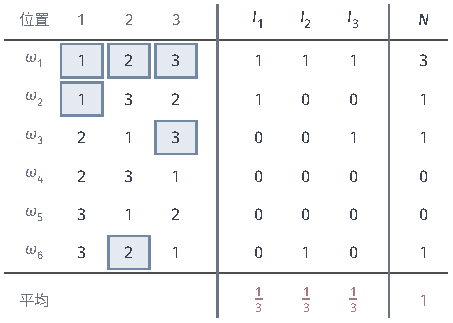
\includegraphics[width=77mm]{figures/07-probability/01-elementary-probability/tikz/rvm-fixed-points/figure.pdf}
 \caption{三封信装入三个信封的六种等可能方式。每行列出各位置装入的信，蓝框表示装对。$I_j$记录第$j$封是否装对，$N=I_1+I_2+I_3$。各列平均（红）满足$\tfrac13+\tfrac13+\tfrac13=1$，尽管$I_1,I_2,I_3$相互依赖。}
 \label{fig:rvm-fixed-points}
\end{BookInlineFigure}

\paragraph{乘积与无穷和}
线性性只涉及加法和数乘。乘积的期望一般不能拆开：取$Y=X$为奖金，则
\[
 \mathbb{E}[XY]=\mathbb{E}[X^{2}]=0\times\tfrac12+9\times\tfrac13+36\times\tfrac16=9,
\]
而$\mathbb{E}[X]\,\mathbb{E}[Y]=4$。乘积可以拆开的充分条件是独立，这需要联合分布，在第~\ref{chap:random-vectors}章讨论。

线性性对有限个变量成立。对无穷多个变量之和，等式
\[
 \mathbb{E}\Bigl[\sum_{k=1}^{\infty}X_k\Bigr]=\sum_{k=1}^{\infty}\mathbb{E}[X_k]
\]
相当于交换求和与取极限的次序，需要非负性或绝对可和这样的额外条件。这类交换的一般依据在第~\ref{chap:probability-spaces}章由积分的收敛定理给出。

\subsection{函数的期望}
\label{sec:rvm-function-expectation}

奖金的平方平均是多少？按定义，应当先求出新变量$Y=X^{2}$的概率表：$Y$取$0,9,36$，概率依次为$\tfrac12,\tfrac13,\tfrac16$，再加权得$9$。上一小节正是这样做的。但这个结果也可以不写出$Y$的分布，直接在$X$的每个取值上计算$x^{2}$再加权。下面的定理说明这种直接计算总是正确的，只要相应的和或积分绝对收敛。

\begin{theorem}[函数的期望]
\label{thm:rvm-lotus}
设$g$是实值函数。
\begin{enumerate}
 \item 若$X$离散，取值$x_i$，且$\sum_i\lvert g(x_i)\rvert\,p_X(x_i)<\infty$，则$g(X)$可积，且
 \begin{equation}
  \mathbb{E}[g(X)]=\sum_{i}g(x_i)\,p_X(x_i) .
  \label{eq:rvm-lotus-discrete}
 \end{equation}
 \item 若$X$有密度$f_X$，$g$分段连续，且$\int_{-\infty}^{\infty}\lvert g(x)\rvert f_X(x)\,\mathrm{d}x<\infty$，则$g(X)$可积，且
 \begin{equation}
  \mathbb{E}[g(X)]=\int_{-\infty}^{\infty}g(x)\,f_X(x)\,\mathrm{d}x .
  \label{eq:rvm-lotus-density}
 \end{equation}
\end{enumerate}
若$g\geq0$，两式在不要求有限的情况下也成立，两边同时为有限数或同时为$+\infty$。
\end{theorem}

\begin{proof}
离散情形。$Y=g(X)$的取值是集合$\{g(x_i)\}$中的数。对每个$y$，事件$\{Y=y\}$是若干个事件$\{X=x_i\}$（$g(x_i)=y$）的并，所以
\[
 p_Y(y)=\sum_{i:\,g(x_i)=y}p_X(x_i) .
\]
代入$Y$的期望，再把对$y$与对$i$的二重和合并成对$i$的一重和，得到
\[
 \sum_{y}y\,p_Y(y)=\sum_{y}\sum_{i:\,g(x_i)=y}g(x_i)\,p_X(x_i)=\sum_{i}g(x_i)\,p_X(x_i) .
\]
最后一步中每个$i$恰好出现在$y=g(x_i)$那一组。对$\lvert g\rvert$作同样的计算，得到
\[
 \mathbb{E}\lvert Y\rvert=\sum_i\lvert g(x_i)\rvert\,p_X(x_i)<\infty,
\]
所以$Y$可积，而绝对收敛保证了上面的重新分组不改变和。$g\geq0$时各项非负，重新分组同样不改变和，结论对$+\infty$也成立。

密度情形只证$g$在$X$的取值区间$(\alpha,\beta)$上连续可微且$g'>0$的情形。这时$g$把$(\alpha,\beta)$一一映成区间$(g(\alpha^{+}),g(\beta^{-}))$，记反函数为$h$。由$\{g(X)\leq y\}=\{X\leq h(y)\}$，
\[
 F_Y(y)=F_X\bigl(h(y)\bigr),\qquad f_Y(y)=f_X\bigl(h(y)\bigr)\,h'(y) .
\]
先设$g\geq0$。在$\int y\,f_Y(y)\,\mathrm{d}y$中作换元$y=g(x)$，$h(y)=x$，$\mathrm{d}y=g'(x)\,\mathrm{d}x$，并利用$h'(g(x))g'(x)=1$，得到
\[
 \int y\,f_X\bigl(h(y)\bigr)h'(y)\,\mathrm{d}y=\int_{\alpha}^{\beta}g(x)\,f_X(x)\,\mathrm{d}x .
\]
被积函数非负，反常积分的换元对有限值和$+\infty$都成立。一般的$g$对正部$g^{+}$与负部$g^{-}$分别使用这一结论再相减。$g'<0$时换元会交换积分上下限，结论相同。
\end{proof}

密度情形的一般证明需要先求出$g(X)$的分布，而$g(X)$可能根本没有密度，例如$g$是指示函数或在某个区间上为常数。第~\ref{chap:random-variable-transformations}章用换元公式处理分段单调的$g$，第~\ref{chap:probability-spaces}章把式~\eqref{eq:rvm-lotus-density}作为推前分布上的积分一般地证明。在这之前，我们在定理的条件下使用它。

定理中的绝对可积条件要对每个$g$分别检查，它与$X$本身是否可积无关。例如密度$f_X(x)=x^{-2}$（$x\geq1$）的$X$满足
\[
 \mathbb{E}[X]=\int_1^{\infty}x\cdot x^{-2}\,\mathrm{d}x=+\infty,
\]
但
\[
 \mathbb{E}\bigl[\sqrt{X}\bigr]=\int_1^{\infty}x^{1/2}\cdot x^{-2}\,\mathrm{d}x=\int_1^{\infty}x^{-3/2}\,\mathrm{d}x=2,
\]
增长较慢的函数仍可积。反过来，$X$可积也不保证$X^{2}$可积，第~\ref{sec:rvm-moments}节会系统地讨论这一点。

\paragraph{指示函数：概率也是期望}
取$g=\mathbf{1}_{A}$，它在$x\in A$时为$1$，否则为$0$。式~\eqref{eq:rvm-lotus-discrete}或式~\eqref{eq:rvm-lotus-density}的右边只剩下$A$上的质量，于是
\begin{equation}
 \mathbb{E}\bigl[\mathbf{1}_{A}(X)\bigr]=\mathbb{P}(X\in A) .
 \label{eq:rvm-indicator}
\end{equation}
概率因此是期望的特殊情形，信封例子中$\mathbb{E}[I_j]=\tfrac13$用的正是这一点。对奖金表取$A=(0,\infty)$，得到中奖的概率$\tfrac13+\tfrac16=\tfrac12$。

\paragraph{收益：不必先求新变量的分布}
奖金本身就是点数的函数。设$D$是骰子点数，$g(1)=g(2)=g(3)=0$，$g(4)=g(5)=3$，$g(6)=6$，则$X=g(D)$。由式~\eqref{eq:rvm-lotus-discrete}，
\[
 \mathbb{E}[g(D)]=\tfrac16\bigl(g(1)+\dots+g(6)\bigr)=\tfrac16(0+0+0+3+3+6)=2,
\]
与先求$X$的概率表再加权的结果相同。若参加一次要付$2.5$元，净收益是$g(D)-2.5$，由线性性它的期望是$-0.5$元，长期参加平均每次亏$0.5$元。

连续的例子也一样。设$X$的密度是$2x$（$0<x<1$），$Y=X^{2}$。直接计算
\[
 \mathbb{E}[X^{2}]=\int_0^1x^{2}\cdot2x\,\mathrm{d}x=\tfrac12 .
\]
另一方面，对$0<y<1$有
\[
 F_Y(y)=\mathbb{P}(X\leq\sqrt{y})=\int_0^{\sqrt{y}}2x\,\mathrm{d}x=y,
\]
所以$Y$在$(0,1)$上有常数密度$1$，$\mathbb{E}[Y]=\int_0^1y\,\mathrm{d}y=\tfrac12$。两条途径对应图~\ref{fig:rvm-square-transform}中两块面积，它们相等。

\begin{BookInlineFigure}
 \centering
 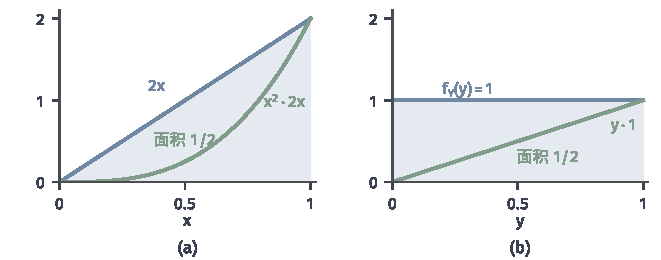
\includegraphics[width=112mm]{figures/07-probability/01-elementary-probability/matplotlib/rvm-square-transform/figure.pdf}
 \caption{用两种方式计算$\mathbb{E}[X^{2}]$，$X$的密度为$2x$。(a)在$X$的尺度上积分$x^{2}\cdot2x$（绿色曲线下的面积）；(b)先求出$Y=X^{2}$的密度$f_Y(y)=1$，再积分$y\cdot1$（绿色直线下的面积）。两块面积都是$1/2$。}
 \label{fig:rvm-square-transform}
\end{BookInlineFigure}

\paragraph{平方误差与绝对误差}
如果要用一个常数$c$预测奖金，平方误差的平均是多少？设$\mathbb{E}[X^{2}]<\infty$，记$\mu=\mathbb{E}[X]$。把$X-c$写成$(X-\mu)+(\mu-c)$后展开，由线性性，交叉项的期望是$2(\mu-c)\,\mathbb{E}[X-\mu]=0$，于是
\begin{equation}
 \mathbb{E}\bigl[(X-c)^{2}\bigr]=\mathbb{E}\bigl[(X-\mu)^{2}\bigr]+(\mu-c)^{2} .
 \label{eq:rvm-square-error}
\end{equation}
右边第二项只在$c=\mu$时为零，所以期望是平方误差意义下最好的常数预测。对奖金表，偏差$X-2$取$-2,1,4$，
\[
 \mathbb{E}\bigl[(X-2)^{2}\bigr]=4\cdot\tfrac12+1\cdot\tfrac13+16\cdot\tfrac16=5,
\]
因此
\[
 \mathbb{E}\bigl[(X-c)^{2}\bigr]=5+(c-2)^{2},
\]
它是图~\ref{fig:rvm-error-curves}(a)中的抛物线，最低点为$(2,5)$。最小值$5$是下一节的方差。

把平方换成绝对值，结论就变了。对奖金表，
\[
 \mathbb{E}\lvert X-c\rvert=\tfrac12\lvert c\rvert+\tfrac13\lvert3-c\rvert+\tfrac16\lvert6-c\rvert .
\]
逐段去掉绝对值：$c<0$时它等于$2-c$，$0\leq c\leq3$时等于常数$2$，$3\leq c\leq6$时等于$\tfrac23c$，$c>6$时等于$c-2$。最小值在整个区间$[0,3]$上取到。这个区间正是使$\mathbb{P}(X\leq c)\geq\tfrac12$且$\mathbb{P}(X\geq c)\geq\tfrac12$的点，即奖金的全部中位数。

\begin{BookInlineFigure}
 \centering
 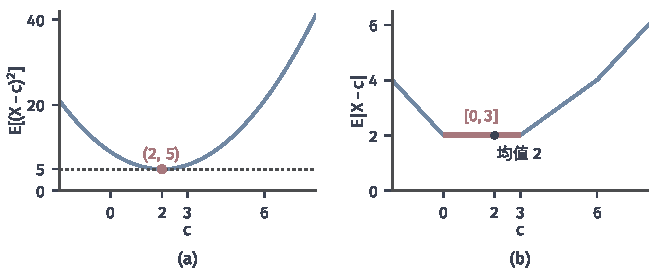
\includegraphics[width=112mm]{figures/07-probability/01-elementary-probability/matplotlib/rvm-error-curves/figure.pdf}
 \caption{用常数$c$预测奖金$X$的平均误差。(a)平方误差$\mathbb{E}[(X-c)^{2}]=5+(c-2)^{2}$在均值$c=2$处取最小值$5$（红点）。(b)绝对误差$\mathbb{E}\lvert X-c\rvert$是折线，在中位数构成的区间$[0,3]$（红色粗线）上取最小值$2$，均值$2$（黑点）恰好也在其中。}
 \label{fig:rvm-error-curves}
\end{BookInlineFigure}

图~\ref{fig:rvm-error-curves}(b)的斜率解释了原因：当$c$不是取值点时，$c$右移一个单位，左侧质量$\mathbb{P}(X<c)$的误差各增加一，右侧质量$\mathbb{P}(X>c)$的误差各减少一，斜率是$\mathbb{P}(X<c)-\mathbb{P}(X>c)$。左右质量相等时斜率为零，这就是中位数的条件。均值与中位数因此回答不同的问题：均值使平方误差最小，受远处取值的影响大；中位数使绝对误差最小，只看质量在左右两侧的分配。若把奖金$6$换成$60$，均值从$2$变成$11$，中位数区间仍是$[0,3]$。

\subsection{凸函数的期望}
\label{sec:rvm-convex-expectation}

先平均再平方，与先平方再平均，结果一样吗？对奖金表，$(\mathbb{E}[X])^{2}=4$，而$\mathbb{E}[X^{2}]=9$。一般地，对非线性函数$f$，$\mathbb{E}[f(X)]$与$f(\mathbb{E}[X])$不相等，但对凸函数两者总有确定的大小关系。这个关系在后面比较风险、比较信息量时反复使用。

\paragraph{有限加权平均}
回忆凸函数的定义：区间$I$上的$f$对一切$x,y\in I$与$\lambda\in[0,1]$满足
\[
 f\bigl(\lambda x+(1-\lambda)y\bigr)\leq\lambda f(x)+(1-\lambda)f(y),
\]
即两点间的图像不高于弦，可参考\BookChapterRef{chap:univariate-differentiation}{卷一第6章“一元函数的微分”}。两点的情形推广到有限个点，就得到下面的引理。

\begin{lemma}[有限加权平均的凸性]
\label{lem:rvm-jensen-finite}
设$f$是区间$I$上的凸函数，点$x_1,\dots,x_n$都在$I$中，权重$\lambda_1,\dots,\lambda_n$非负且和为一。则
\begin{equation}
 f\Bigl(\sum_{i=1}^{n}\lambda_ix_i\Bigr)\leq\sum_{i=1}^{n}\lambda_if(x_i) .
 \label{eq:rvm-jensen-finite}
\end{equation}
\end{lemma}

\begin{proof}
对$n$归纳。$n=1$时两边相等，$n=2$时就是凸函数的定义。设结论对$n-1$个点成立。若$\lambda_n=1$，其余权重都为零，结论成立。否则记$s=1-\lambda_n>0$，令
\[
 \bar{x}=\sum_{i=1}^{n-1}\frac{\lambda_i}{s}x_i .
\]
权重$\lambda_i/s$非负且和为一，$\bar{x}$是$I$中点的加权平均，仍在区间$I$中，并且$\sum_{i}\lambda_ix_i=s\bar{x}+\lambda_nx_n$。先用两点的凸性，再对$\bar{x}$用归纳假设，得到
\[
 f\bigl(s\bar{x}+\lambda_nx_n\bigr)\leq sf(\bar{x})+\lambda_nf(x_n)\leq s\sum_{i=1}^{n-1}\frac{\lambda_i}{s}f(x_i)+\lambda_nf(x_n),
\]
右边等于$\sum_{i=1}^{n}\lambda_if(x_i)$。
\end{proof}

引理有一个直观的重心解释。把质量$\lambda_i$放在图像上的点$(x_i,f(x_i))$，这组质量的重心是$\bigl(\sum\lambda_ix_i,\sum\lambda_if(x_i)\bigr)$，它落在这些点的凸包内。凸函数的图像向下弯，凸包整个位于图像上方或图像上，所以重心的高度不低于图像在同一横坐标处的高度。图~\ref{fig:rvm-jensen}(a)用奖金表画出了这一点：三个点$(0,0)$、$(3,9)$、$(6,36)$的重心是$(2,9)$，图像在$x=2$处的高度只有$4$。

\paragraph{支撑线}
推广到可数个取值和密度时，不能再逐点归纳，需要另一个工具：在凸函数图像上任一内点处，总可以放一条不高于图像的直线。

\begin{lemma}[凸函数的支撑线]
\label{lem:rvm-support-line}
设$f$是开区间$I$上的凸函数，$m\in I$。存在实数$s$，使对一切$x\in I$，
\begin{equation}
 f(x)\geq f(m)+s(x-m) .
 \label{eq:rvm-support-line}
\end{equation}
若$f$在$m$处可微，可取$s=f'(m)$。若$f$严格凸，则$x\neq m$时不等式严格成立。
\end{lemma}

\begin{proof}
取$x<m<y$，均在$I$中。把$m$写成$x$与$y$的凸组合，由凸性得到弦的斜率关系
\[
 \frac{f(m)-f(x)}{m-x}\leq\frac{f(y)-f(m)}{y-m},
\]
这正是上面所引可微凸函数刻画的证明第一步，那一步没有用到可微性。上式对一切$x<m$与$y>m$成立，所以左边对$x$的上确界$L$不超过右边对$y$的下确界$R$，两者都是有限数。取$s\in[L,R]$。对$x<m$，由$\frac{f(m)-f(x)}{m-x}\leq s$得$f(x)\geq f(m)+s(x-m)$；对$y>m$，由$\frac{f(y)-f(m)}{y-m}\geq s$得同一不等式。可微时左右两侧的斜率都趋于$f'(m)$，所以$L=R=f'(m)$。

若$f$严格凸，假设某个$x\neq m$使等号成立，不妨设$x>m$。$f$在$x$与$m$处都与直线$\ell(t)=f(m)+s(t-m)$相等，取中点$z=(x+m)/2$，严格凸性给出$f(z)<\frac12f(m)+\frac12f(x)=\ell(z)$，与$f\geq\ell$矛盾。
\end{proof}

\paragraph{Jensen不等式}
有了支撑线，在$m=\mathbb{E}[X]$处放一条支撑线再取期望，就得到对一般随机变量成立的不等式。

\begin{theorem}[Jensen不等式]
\label{thm:rvm-jensen}
设$f$是开区间$I$上的凸函数，$X$的取值都在$I$中，$X$与$f(X)$都可积。则$\mathbb{E}[X]\in I$，且
\begin{equation}
 f\bigl(\mathbb{E}[X]\bigr)\leq\mathbb{E}\bigl[f(X)\bigr] .
 \label{eq:rvm-jensen}
\end{equation}
若$f$严格凸，等号成立当且仅当$X$以概率一等于常数$\mathbb{E}[X]$。
\end{theorem}

\begin{proof}
先说明$m=\mathbb{E}[X]$在$I$中。设$I$的左端点$\alpha$有限，$X-\alpha$的取值都为正。离散时，$\mathbb{E}[X]-\alpha=\sum_i(x_i-\alpha)p_X(x_i)$中各项非负且总有正项；有密度时，被积函数$(x-\alpha)f_X(x)$非负，且$X$落在某个$[\alpha+\delta,\infty)$中的概率为正，于是积分至少是$\delta$乘这个概率。两种情形都有$m>\alpha$。右端点同理，所以$m\in I$。

由引理~\ref{lem:rvm-support-line}，存在$s$使$f(x)\geq f(m)+s(x-m)$对一切$x\in I$成立。把$x$换成$X$，两边都是可积的随机变量，由保序性与线性性，
\[
 \mathbb{E}[f(X)]\geq f(m)+s\bigl(\mathbb{E}[X]-m\bigr)=f(m) .
\]

等号情形。记$D(x)=f(x)-f(m)-s(x-m)\geq0$，则$\mathbb{E}[D(X)]=\mathbb{E}[f(X)]-f(m)$。$f$严格凸时，$x\neq m$有$D(x)>0$。若$X$离散且$\mathbb{P}(X\neq m)>0$，和式$\sum_iD(x_i)\,p_X(x_i)$中有正项，所以$\mathbb{E}[D(X)]>0$。若$X$有密度，单点$m$的概率为零，总可以找到一个不含$m$的闭区间，使$X$落在其中的概率为正；凸函数在开区间上连续，$D$在这个闭区间上有正的最小值，于是$\mathbb{E}[D(X)]>0$。反过来，$X$以概率一等于$m$时$f(X)$以概率一等于$f(m)$，两边相等。
\end{proof}

定理的条件各有用处。区间取开区间，是为了让$m$成为内点，从而支撑线存在；在闭区间的端点处，凸函数可能没有有限斜率的支撑线，例如$-\sqrt{x}$在$0$处。$X$与$f(X)$可积，保证了取期望时两边都是有限数并可以用线性性。若$f(X)$只是非负而期望为$+\infty$，不等式按$+\infty$理解仍然成立。

\begin{BookInlineFigure}
 \centering
 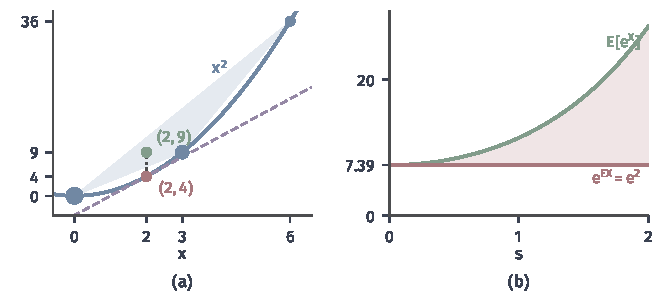
\includegraphics[width=112mm]{figures/07-probability/01-elementary-probability/matplotlib/rvm-jensen/figure.pdf}
 \caption{Jensen不等式的几何。(a)$f(x)=x^{2}$与奖金表：蓝点$(x_i,x_i^{2})$按概率大小画出，浅蓝三角是它们的凸包，重心$(\mathbb{E}[X],\mathbb{E}[X^{2}])=(2,9)$（绿）高于$(2,f(2))=(2,4)$（红）；紫色虚线是$x=2$处的支撑线$y=4+4(x-2)$。(b)$X$以各$\tfrac12$的概率取$2\pm s$时，$\mathbb{E}[\mathrm{e}^{X}]=\mathrm{e}^{2}\cosh s$（绿）与$\mathrm{e}^{\mathbb{E}[X]}=\mathrm{e}^{2}$（红）之差（浅红）随$s$增大。}
 \label{fig:rvm-jensen}
\end{BookInlineFigure}

\paragraph{平方、指数与对数}
取$f(x)=x^{2}$，它在$\mathbb{R}$上严格凸，Jensen不等式给出$(\mathbb{E}[X])^{2}\leq\mathbb{E}[X^{2}]$。差值$\mathbb{E}[X^{2}]-(\mathbb{E}[X])^{2}$就是式~\eqref{eq:rvm-square-error}中$c=0$时多出的那一项$\mathbb{E}[(X-\mu)^{2}]$，它衡量$X$偏离均值的程度。奖金表的差值是$9-4=5$。

取$f(x)=\mathrm{e}^{x}$。对密度$2x$，分部积分得
\[
 \mathbb{E}[\mathrm{e}^{X}]=\int_0^12x\,\mathrm{e}^{x}\,\mathrm{d}x=\Bigl[2(x-1)\mathrm{e}^{x}\Bigr]_0^1=2,
\]
而$\mathrm{e}^{2/3}\approx1.948$，差值只有约$0.05$。差值小，是因为$X$集中在长度为$1$的区间里，指数函数在这么短的区间上接近一条直线。图~\ref{fig:rvm-jensen}(b)取两点分布$2\pm s$，差值$\mathrm{e}^{2}(\cosh s-1)$随分散程度$s$迅速增大：变量越分散，凸函数的弯曲被平均放大得越多。

对凹函数，不等号反向。$\ln x$在$(0,\infty)$上严格凹，所以$\mathbb{E}[\ln X]\leq\ln\mathbb{E}[X]$。对密度$2x$，
\[
 \mathbb{E}[\ln X]=\int_0^12x\ln x\,\mathrm{d}x=\Bigl[x^{2}\ln x-\tfrac{x^{2}}{2}\Bigr]_0^1=-\tfrac12,
\]
而$\ln\tfrac23\approx-0.405$，确实更大。第~\ref{chap:information-measures}章研究信息量时，正是用对数的凹性证明各种信息量非负。

\paragraph{不是凸函数时}
若$f$既不凸也不凹，两边的大小关系由分布决定。取$f(x)=x^{3}$。奖金表给出
\[
 \mathbb{E}[X^{3}]=27\cdot\tfrac13+216\cdot\tfrac16=45>2^{3}=8 .
\]
把奖金变号，$-X$的三次方平均是$-45$，小于$(-2)^{3}=-8$。以各$\tfrac12$的概率取$\pm1$时两边都是$0$。所以Jensen不等式中凸性不能省略，它决定了不等号的方向。


\section{方差}
\label{sec:rvm-variance}

两个游戏平均奖金都是$2$元，一个总是恰好给$2$元，另一个有一半机会一分不得、偶尔给$6$元。期望看不出这种差别。我们需要第二个数，衡量取值在均值周围散开的程度。上一节的平方误差已经给出了候选：用均值预测时的平均平方误差。本节把它定义为方差，说明存在条件、计算方法和它在平移、缩放下的变化，再由它得到与原变量同单位的标准差。

\subsection{定义}
\label{sec:rvm-variance-definition}

\paragraph{三个均值相同的游戏}
比较三张均值都是$2$的概率表：(a)恒取$2$；(b)以各$\tfrac12$的概率取$1$或$3$；(c)奖金表，以$\tfrac12,\tfrac13,\tfrac16$的概率取$0,3,6$。图~\ref{fig:rvm-same-mean}中三者的重心都在$2$，质量离重心的远近却明显不同。

怎样把“离重心多远”变成一个数？最直接的想法是平均偏差$\mathbb{E}[X-\mu]$，但由线性性它恒等于$\mathbb{E}[X]-\mu=0$：正负偏差正好抵消，这正是重心的定义。要避免抵消，可以取绝对值$\mathbb{E}\lvert X-\mu\rvert$，也可以取平方$\mathbb{E}[(X-\mu)^{2}]$。平方的好处是能展开：上一节的式~\eqref{eq:rvm-square-error}就是靠展开得到的，后面的计算公式、平移缩放规律以及第~\ref{chap:random-vectors}章和的方差都依赖这一点。

\begin{BookInlineFigure}
 \centering
 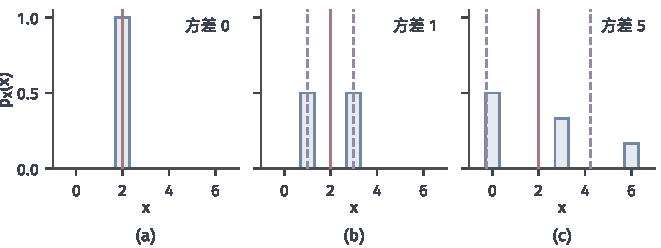
\includegraphics[width=112mm]{figures/07-probability/01-elementary-probability/matplotlib/rvm-same-mean/figure.pdf}
 \caption{三张均值都是$2$的概率表。(a)恒取$2$；(b)以各$\tfrac12$的概率取$1,3$；(c)奖金表。红线是均值，紫色虚线是均值加减标准差$\sqrt{\operatorname{Var}(X)}$。均值相同，方差依次为$0,1,5$。}
 \label{fig:rvm-same-mean}
\end{BookInlineFigure}

力学里也有同样的量。把单位质量按概率放在数轴上，到重心距离的平方乘质量再求和，就是这组质量绕重心的转动惯量。质量离重心越远，转动惯量越大，转动起来越费力。图~\ref{fig:rvm-variance-squares}把奖金表的每个偏差画成正方形，转动惯量就是这些正方形面积的概率加权和。这个类比在一处不完全对应：物理的转动惯量对任何有限质量分布都有限，而概率质量可以分布到无穷远，平方加权和可能是$+\infty$。

\begin{BookInlineFigure}
 \centering
 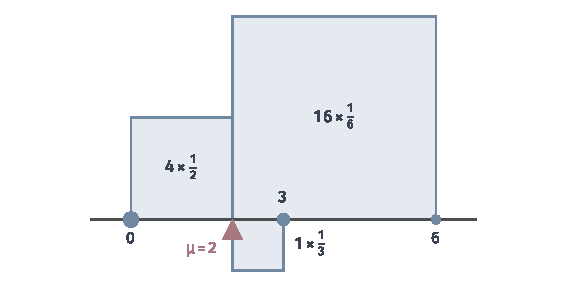
\includegraphics[width=96mm]{figures/07-probability/01-elementary-probability/matplotlib/rvm-variance-squares/figure.pdf}
 \caption{奖金表的方差是偏差平方的加权平均。三个取值到均值$\mu=2$的距离是$2,1,4$，对应正方形的面积是$4,1,16$（为避免重叠，$x=3$的正方形画在数轴下方），蓝点大小表示概率。按概率加权，$4\times\tfrac12+1\times\tfrac13+16\times\tfrac16=5$。}
 \label{fig:rvm-variance-squares}
\end{BookInlineFigure}

\paragraph{方差的定义}
平方的平均有意义，需要先有均值，并且平方的加权和有限。下面的定义把这两项要求都放在“$X^{2}$的期望有限”这一个条件里。

\begin{definition}[方差]
\label{def:rvm-variance}
设$\mathbb{E}[X^{2}]<\infty$，记$\mu=\mathbb{E}[X]$。称
\begin{equation}
 \operatorname{Var}(X)=\mathbb{E}\bigl[(X-\mu)^{2}\bigr]
 \label{eq:rvm-variance}
\end{equation}
为$X$的\term{方差}（variance），也记作$\sigma^{2}$或$\sigma_X^{2}$。
\end{definition}

条件$\mathbb{E}[X^{2}]<\infty$同时保证了均值有限和方差有限。由$(\lvert x\rvert-1)^{2}\geq0$得$\lvert x\rvert\leq\frac12(1+x^{2})$，所以
\[
 \mathbb{E}\lvert X\rvert\leq\tfrac12\bigl(1+\mathbb{E}[X^{2}]\bigr)<\infty .
\]
再由$(x-\mu)^{2}\leq2x^{2}+2\mu^{2}$，又得到
\[
 \mathbb{E}\bigl[(X-\mu)^{2}\bigr]\leq2\,\mathbb{E}[X^{2}]+2\mu^{2}<\infty .
\]这两步都是函数期望的比较，用到了保序性。

均值有限并不保证方差有限。密度$f_X(x)=2x^{-3}$（$x\geq1$）的均值是
\[
 \mathbb{E}[X]=\int_1^{\infty}x\cdot2x^{-3}\,\mathrm{d}x=2,
\]
但
\[
 \mathbb{E}[X^{2}]=\int_1^{\infty}x^{2}\cdot2x^{-3}\,\mathrm{d}x=\int_1^{\infty}\frac{2}{x}\,\mathrm{d}x=+\infty .
\]这时$(X-2)^{2}$是非负变量，它的期望按定义~\ref{def:rvm-expectation}等于$+\infty$，我们说$X$的方差无穷或不是有限的。远处的质量衰减得足以使一次方的力矩有限，却不足以使平方的力矩有限。

图~\ref{fig:rvm-same-mean}中三张表的方差分别是
\[
 0,\qquad (1-2)^{2}\cdot\tfrac12+(3-2)^{2}\cdot\tfrac12=1,\qquad 4\cdot\tfrac12+1\cdot\tfrac13+16\cdot\tfrac16=5 .
\]
方差的大小顺序与图中质量散开的程度一致。

\paragraph{方差为零}
方差是非负变量的期望，所以$\operatorname{Var}(X)\geq0$。方差为零意味着什么？它与“均值是某个数”不是一回事：图~\ref{fig:rvm-same-mean}中三张表的均值都是$2$，只有(a)的方差为零。下面说明方差为零恰好刻画了取值不变的变量。

\begin{theorem}[方差为零的变量]
\label{thm:rvm-zero-variance}
设$\mathbb{E}[X^{2}]<\infty$，$\mu=\mathbb{E}[X]$。
\begin{enumerate}
 \item 若$X$离散，则$\operatorname{Var}(X)=0$当且仅当$\mathbb{P}(X=\mu)=1$。
 \item 若$X$有密度，则$\operatorname{Var}(X)>0$。
\end{enumerate}
\end{theorem}

\begin{proof}
离散情形。$\operatorname{Var}(X)=\sum_i(x_i-\mu)^{2}p_X(x_i)$是非负项之和，它为零当且仅当每个$p_X(x_i)>0$的取值都满足$x_i=\mu$，即全部概率都在$\mu$上。

密度情形。取$\delta>0$，记$A_{\delta}=\{x:\lvert x-\mu\rvert\geq\delta\}$。在$A_{\delta}$上被积函数$(x-\mu)^{2}f_X(x)\geq\delta^{2}f_X(x)$，其余部分非负，所以
\[
 \operatorname{Var}(X)\geq\delta^{2}\int_{A_{\delta}}f_X(x)\,\mathrm{d}x=\delta^{2}\Bigl(1-\int_{\mu-\delta}^{\mu+\delta}f_X(x)\,\mathrm{d}x\Bigr) .
\]
$\delta\to0$时，长度趋于零的区间上的积分趋于零，所以对足够小的$\delta$，括号内大于$\tfrac12$，右边为正。
\end{proof}

这个结论把“数值恒定”说得很准确。方差为零的离散变量以概率一等于均值；若样本空间中还有概率为零的样本点，变量在那里可以取别的值，但这不影响任何概率和期望。有密度的变量把质量铺在一段长度上，不可能全部集中在一点，方差必然为正。对一般的随机变量，同样的刻画在第~\ref{chap:probability-spaces}章证明。

\subsection{计算}
\label{sec:rvm-variance-computation}

按定义计算方差需要两步：先求均值$\mu$，再对$(x-\mu)^{2}$加权求和或积分。对概率表与密度，两个公式分别是
\begin{equation}
 \operatorname{Var}(X)=\sum_{i}(x_i-\mu)^{2}p_X(x_i),\qquad
 \operatorname{Var}(X)=\int_{-\infty}^{\infty}(x-\mu)^{2}f_X(x)\,\mathrm{d}x .
 \label{eq:rvm-variance-formulas}
\end{equation}
它们是函数期望定理~\ref{thm:rvm-lotus}取$g(x)=(x-\mu)^{2}$的特殊情形。对密度$2x$，$\mu=\tfrac23$，展开被积函数后逐项积分，得到
\[
 \operatorname{Var}(X)=\int_0^12x\Bigl(x^{2}-\tfrac43x+\tfrac49\Bigr)\mathrm{d}x
 =2\Bigl(\tfrac14-\tfrac49+\tfrac29\Bigr)=\tfrac{1}{18} .
\]

把展开放在期望外面做，就得到一个通常更方便的公式，它只需要$\mathbb{E}[X]$与$\mathbb{E}[X^{2}]$。

\begin{theorem}[方差的展开式]
\label{thm:rvm-variance-shortcut}
设$\mathbb{E}[X^{2}]<\infty$，则
\begin{equation}
 \operatorname{Var}(X)=\mathbb{E}[X^{2}]-\bigl(\mathbb{E}[X]\bigr)^{2} .
 \label{eq:rvm-variance-shortcut}
\end{equation}
\end{theorem}

\begin{proof}
记$\mu=\mathbb{E}[X]$。$(X-\mu)^{2}=X^{2}-2\mu X+\mu^{2}$，右边三项都可积。由线性性，
\[
 \mathbb{E}\bigl[(X-\mu)^{2}\bigr]=\mathbb{E}[X^{2}]-2\mu\,\mathbb{E}[X]+\mu^{2}=\mathbb{E}[X^{2}]-\mu^{2} .
\]
\end{proof}

用展开式重算两个贯穿例子。奖金表的$\mathbb{E}[X^{2}]=9$，$\mathbb{E}[X]=2$，于是$\operatorname{Var}(X)=9-4=5$。密度$2x$的$\mathbb{E}[X^{2}]=\tfrac12$已在函数期望中算过，于是
\[
 \operatorname{Var}(X)=\tfrac12-\Bigl(\tfrac23\Bigr)^{2}=\tfrac{9-8}{18}=\tfrac{1}{18} .
\]
两个结果都与按定义计算的一致。由于方差非负，式~\eqref{eq:rvm-variance-shortcut}也重新给出了$\mathbb{E}[X^{2}]\geq(\mathbb{E}[X])^{2}$，这是\term{Jensen不等式}在$f(x)=x^{2}$时的情形。

把式~\eqref{eq:rvm-variance-shortcut}与上一节的式~\eqref{eq:rvm-square-error}放在一起，得到对任意常数$c$成立的分解
\begin{equation}
 \mathbb{E}\bigl[(X-c)^{2}\bigr]=\operatorname{Var}(X)+(\mathbb{E}[X]-c)^{2} .
 \label{eq:rvm-parallel-axis}
\end{equation}
用转动惯量的语言，它说绕任一点$c$的转动惯量等于绕重心的转动惯量加上重心到$c$的距离平方，这是力学中的平行轴定理。图~\ref{fig:rvm-error-curves}(a)中抛物线的最低值$5$就是奖金表的方差。

\paragraph{两种算法的比较}
按定义计算时，每一项$(x_i-\mu)^{2}$都非负，结果天然非负，但必须先算出$\mu$再回头处理每个取值；展开式只需要分别累计$x_i$与$x_i^{2}$的加权和，一遍就能完成，求积分时常常也更简单。代价在于展开式是两个可能很大的数相减。

把奖金表的每个取值都加上$10^{8}$，方差仍是$5$。用双精度浮点数计算，$\mathbb{E}[X^{2}]$与$(\mathbb{E}[X])^{2}$都约为$10^{16}$，而这个量级上相邻两个浮点数相差$2$，两数之差只剩下很少的有效数字。实际计算得到$4$；平移量增大到$10^{9}$时，展开式给出$0$。按定义先减去均值再平方，两种平移下得到的都是$5$。所以手算或求解析式时常用展开式，而均值相对波动很大的数值计算应先中心化。

\subsection{平移与缩放}
\label{sec:rvm-variance-affine}

参加一次奖金游戏要付$2$元，净收益是$X-2$；把赌注加倍，奖金变成$2X$；站在庄家一边，收益是$-X$。这些变量的方差与$X$的方差有什么关系？它们都是$aX+b$的形式，答案由中心化后的偏差决定。

\begin{theorem}[方差的平移与缩放]
\label{thm:rvm-variance-affine}
设$\mathbb{E}[X^{2}]<\infty$，$a,b$为实数。则$\mathbb{E}[(aX+b)^{2}]<\infty$，且
\begin{equation}
 \mathbb{E}[aX+b]=a\,\mathbb{E}[X]+b,\qquad \operatorname{Var}(aX+b)=a^{2}\operatorname{Var}(X) .
 \label{eq:rvm-variance-affine}
\end{equation}
\end{theorem}

\begin{proof}
$(ax+b)^{2}\leq2a^{2}x^{2}+2b^{2}$，所以$(aX+b)^{2}$可积。均值的公式是线性性。记$\mu=\mathbb{E}[X]$，新变量的偏差是
\[
 (aX+b)-(a\mu+b)=a(X-\mu),
\]
平移量$b$在相减时消去。平方后取期望，得到
\[
 \operatorname{Var}(aX+b)=\mathbb{E}\bigl[a^{2}(X-\mu)^{2}\bigr]=a^{2}\operatorname{Var}(X) .
\]
\end{proof}

平移整体移动所有取值，不改变它们之间的距离，所以方差不变；缩放把每个偏差乘以$a$，平方后方差乘以$a^{2}$。图~\ref{fig:rvm-shift-scale}画出了奖金表的三个变换：$X-2$的均值是$0$，方差仍是$5$；$2X$的均值是$4$，方差是$4\times5=20$；$-X$把分布左右翻转，均值是$-2$，方差仍是$5$，因为$(-1)^{2}=1$。

\begin{BookInlineFigure}
 \centering
 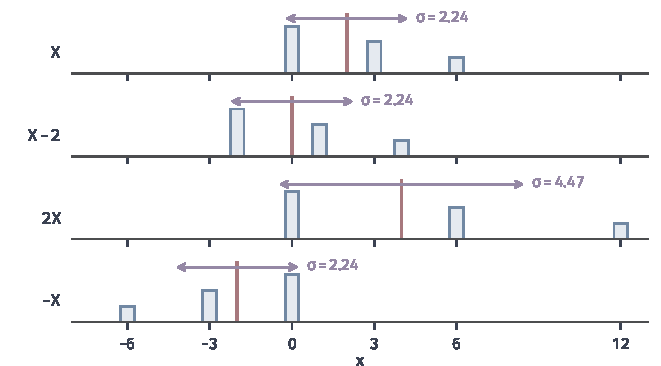
\includegraphics[width=112mm]{figures/07-probability/01-elementary-probability/matplotlib/rvm-shift-scale/figure.pdf}
 \caption{奖金表$X$及其平移、缩放与反射。红线是均值，紫色双箭头是均值加减一个标准差。$X-2$整体左移，宽度不变；$2X$的取值间距加倍，标准差从$2.24$变为$4.47$；$-X$左右翻转，标准差不变。}
 \label{fig:rvm-shift-scale}
\end{BookInlineFigure}

两个特殊情形值得核对。$a=0$时$aX+b$是常数$b$，公式给出方差$0$，与定理~\ref{thm:rvm-zero-variance}一致。$a<0$时缩放同时带来反射，方差只与$\lvert a\rvert$有关，波动的大小不区分方向。

式~\eqref{eq:rvm-variance-affine}只处理一个变量的线性函数。两个不同变量相加时，偏差的平方会产生交叉项。例如$X+X=2X$的方差是$4\operatorname{Var}(X)=20$，而不是$\operatorname{Var}(X)+\operatorname{Var}(X)=10$，多出的$10$正来自交叉项$2\,\mathbb{E}[(X-\mu)(X-\mu)]$。一般的和的方差由协方差描述，在第~\ref{chap:random-vectors}章计算。

\subsection{标准差与标准化}
\label{sec:rvm-standardization}

奖金以元为单位，方差的单位却是“平方元”，$5$平方元很难与$2$元的均值直接比较。开平方就回到原来的单位。

\begin{definition}[标准差]
\label{def:rvm-std}
设$\mathbb{E}[X^{2}]<\infty$。称方差的非负平方根
\begin{equation}
 \sigma_X=\sqrt{\operatorname{Var}(X)}
 \label{eq:rvm-std}
\end{equation}
为$X$的\term{标准差}（standard deviation）。
\end{definition}

奖金表的标准差是$\sqrt5\approx2.24$元，密度$2x$的标准差是$1/\sqrt{18}\approx0.236$。由式~\eqref{eq:rvm-variance-affine}，$\sigma_{aX+b}=\lvert a\rvert\sigma_X$：标准差与变量同步缩放，单位换算时直接乘以换算系数。标准差可以解读为偏差的典型大小，但它是平方平均的平方根，不是平均偏差：奖金表的$\mathbb{E}\lvert X-2\rvert=2$，比$\sqrt5$小，因为平方放大了远处那个偏差$4$的分量。偏离均值超过若干个标准差的概率有多大，要用第~\ref{chap:tail-probabilities}章的尾概率工具估计。

\paragraph{标准化}
均值和标准差分别给出位置和尺度。把它们都除去，就得到一个与单位和位置无关的变量，便于比较不同量纲的随机量，或者描述“偏离均值多少个标准差”。

\begin{definition}[标准化]
\label{def:rvm-standardize}
设$\mathbb{E}[X^{2}]<\infty$且$\sigma_X>0$，$\mu=\mathbb{E}[X]$。称
\begin{equation}
 Z=\frac{X-\mu}{\sigma_X}
 \label{eq:rvm-standardize}
\end{equation}
为$X$的\term{标准化}（standardization）。由式~\eqref{eq:rvm-variance-affine}取$a=1/\sigma_X$，$b=-\mu/\sigma_X$，得$\mathbb{E}[Z]=0$，$\operatorname{Var}(Z)=1$。
\end{definition}

两个条件都不能少。方差必须有限，否则没有可除的尺度；方差必须为正，常数变量没有波动，无法放大成方差为一的变量。

对奖金表，$Z=(X-2)/\sqrt5$以概率$\tfrac12,\tfrac13,\tfrac16$取
\[
 -\tfrac{2}{\sqrt5}\approx-0.89,\qquad \tfrac{1}{\sqrt5}\approx0.45,\qquad \tfrac{4}{\sqrt5}\approx1.79 .
\]
直接核对均值与方差：
\[
 \mathbb{E}[Z]=\tfrac{1}{\sqrt5}\bigl(-1+\tfrac13+\tfrac23\bigr)=0,\qquad
 \mathbb{E}[Z^{2}]=\tfrac15\bigl(2+\tfrac13+\tfrac83\bigr)=1 .
\]对密度$2x$，$Z=\sqrt{18}\,(X-\tfrac23)$的取值范围是$(-2\sqrt2,\sqrt2)$。

\begin{BookInlineFigure}
 \centering
 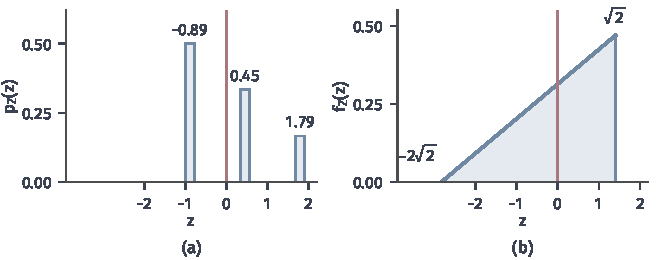
\includegraphics[width=112mm]{figures/07-probability/01-elementary-probability/matplotlib/rvm-standardized/figure.pdf}
 \caption{标准化不改变分布的形状。(a)奖金表标准化后的概率表；(b)密度$2x$标准化后的密度，支撑为$(-2\sqrt2,\sqrt2)$。两者均值都是$0$（红线）、方差都是$1$，但一个是右侧拖尾的三点分布，一个是向右上升的三角形，都不是钟形。}
 \label{fig:rvm-standardized}
\end{BookInlineFigure}

图~\ref{fig:rvm-standardized}说明标准化只做平移和正的缩放，概率表的相对位置和密度的形状都原样保留。均值为零、方差为一并不意味着分布接近某个特定形状，标准化后的奖金仍然只取三个值，仍然向右偏。许多独立小扰动之和标准化后才会接近钟形，那是第~\ref{chap:central-limit-theorem}章的定理，需要独立性和求和，不是标准化本身的效果。


\section{矩}
\label{sec:rvm-moments}

均值是$X$的期望，方差是$(X-\mu)^{2}$的期望。把一次方、二次方换成更高的幂，就得到一族数值特征。奖金表与密度$2x$的均值和方差都已算出，但前者向右拖着一个远处的取值，后者的质量堆在右端，这样的形状差别要靠三次、四次的平均来记录。本节先区分几种矩，再讨论它们何时存在、怎样计算，最后用标准化的三阶和四阶矩描述偏斜与尾部，并说明有限个矩能刻画分布到什么程度。

\subsection{定义}
\label{sec:rvm-moment-definition}

幂次不同，平均对偏差的处理方式也不同。奇数次幂保留偏差的符号，正负偏差会相互抵消；偶数次幂和绝对值的幂不分方向，只记偏差的大小。幂次越高，远处的取值占的权重越大：图~\ref{fig:rvm-power-weights}(a)中$\lvert x\rvert^{p}$在$\lvert x\rvert<1$时随$p$增大而变小，在$\lvert x\rvert>1$时随$p$增大而迅速变大。

\begin{definition}[矩]
\label{def:rvm-moments}
设$k$是正整数，$p>0$是实数。
\begin{enumerate}
 \item 若$\mathbb{E}\lvert X\rvert^{k}<\infty$，称
 \begin{equation}
  m_k=\mathbb{E}[X^{k}]
  \label{eq:rvm-raw-moment}
 \end{equation}
 为$X$的$k$阶\term{原点矩}（raw moment）。
 \item 若$\mathbb{E}\lvert X\rvert^{k}<\infty$，记$\mu=\mathbb{E}[X]$，称
 \begin{equation}
  c_k=\mathbb{E}\bigl[(X-\mu)^{k}\bigr]
  \label{eq:rvm-central-moment}
 \end{equation}
 为$X$的$k$阶\term{中心矩}（central moment）。
 \item 称
 \begin{equation}
  \mathbb{E}\lvert X\rvert^{p}\in[0,+\infty]
  \label{eq:rvm-absolute-moment}
 \end{equation}
 为$X$的$p$阶\term{绝对矩}（absolute moment）；$\mathbb{E}\lvert X-\mu\rvert^{p}$称为$p$阶绝对中心矩。
\end{enumerate}
这些量统称为\term{矩}（moment）。
\end{definition}

在这套记号下，均值是$m_1$，方差是$c_2$，并且$c_1=0$。三类矩的存在条件不同。绝对矩是非负变量的期望，总有意义，只是可能为$+\infty$；阶数$p$可以是任意正实数，例如$\mathbb{E}\lvert X\rvert^{1/2}$。原点矩和中心矩是有符号变量的期望，要求相应的绝对矩有限，阶数取正整数，使$x^{k}$对负数也有定义。中心矩还需要先有均值；下一小节将说明，$\mathbb{E}\lvert X\rvert^{k}<\infty$（$k\geq1$）已经保证了均值有限，也保证了$(X-\mu)^{k}$可积。

\begin{BookInlineFigure}
 \centering
 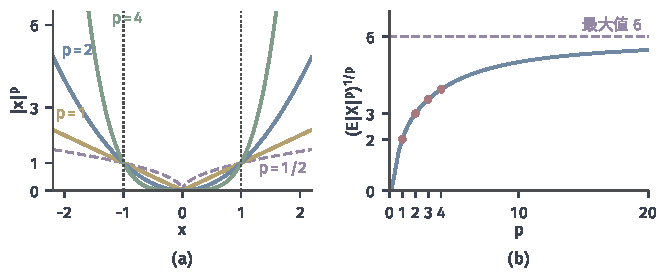
\includegraphics[width=112mm]{figures/07-probability/01-elementary-probability/matplotlib/rvm-power-weights/figure.pdf}
 \caption{幂次与权重。(a)$\lvert x\rvert^{p}$在$p=\tfrac12,1,2,4$时的图像：$\lvert x\rvert<1$时幂次越高权重越小，$\lvert x\rvert>1$时越大，所有曲线在$\lvert x\rvert=1$处（点线）相交。(b)奖金表的$(\mathbb{E}\lvert X\rvert^{p})^{1/p}$随$p$单调增加（蓝），红点是$p=1,2,3,4$时的值$2,3,3.56,3.95$，$p\to\infty$时趋于最大取值$6$（紫色虚线）。}
 \label{fig:rvm-power-weights}
\end{BookInlineFigure}

\paragraph{贯穿例子的矩}
奖金表只取有限个值，各阶矩都存在。由函数期望公式，
\[
 \begin{gathered}
 m_1=2,\qquad m_2=9,\\
 m_3=27\cdot\tfrac13+216\cdot\tfrac16=45,\qquad m_4=81\cdot\tfrac13+1296\cdot\tfrac16=243 .
 \end{gathered}
\]
它的中心矩可以直接从偏差$-2,1,4$计算，例如
\[
 c_3=(-2)^{3}\cdot\tfrac12+1^{3}\cdot\tfrac13+4^{3}\cdot\tfrac16=-4+\tfrac13+\tfrac{32}{3}=7 .
\]
原点矩全为正，因为奖金非负；三阶中心矩为正，是因为偏差$4$的立方$64$远大于偏差$-2$的立方的绝对值$8$，即使后者的概率是前者的三倍。

\subsection{存在性}
\label{sec:rvm-moment-existence}

方差的定义要求$\mathbb{E}[X^{2}]<\infty$，并说明了这一条件蕴含均值有限。同样的道理对一般的阶都成立：高阶矩有限，低阶矩必然有限。

\begin{theorem}[矩的单调存在性]
\label{thm:rvm-moment-monotone}
设$0<p<q$。若$\mathbb{E}\lvert X\rvert^{q}<\infty$，则
\begin{equation}
 \mathbb{E}\lvert X\rvert^{p}\leq1+\mathbb{E}\lvert X\rvert^{q}<\infty .
 \label{eq:rvm-moment-monotone}
\end{equation}
\end{theorem}

\begin{proof}
对每个实数$x$有$\lvert x\rvert^{p}\leq1+\lvert x\rvert^{q}$：若$\lvert x\rvert\leq1$，则$\lvert x\rvert^{p}\leq1$；若$\lvert x\rvert>1$，则$\lvert x\rvert^{p}<\lvert x\rvert^{q}$。把$x$换成$X$并取期望，由保序性即得。
\end{proof}

证明把数轴分成两部分处理。在$\lvert x\rvert\leq1$的近处，所有幂都不超过$1$，总质量又是$1$，所以近处的贡献总是有限的；矩是否存在完全取决于远处，而在远处高次幂压过低次幂。于是$\mathbb{E}\lvert X\rvert^{k}<\infty$蕴含$\mathbb{E}\lvert X\rvert<\infty$，均值存在；再由不等式
\[
 \lvert x-\mu\rvert^{k}\leq2^{k-1}\bigl(\lvert x\rvert^{k}+\lvert\mu\rvert^{k}\bigr),
\]
$(X-\mu)^{k}$也可积，中心矩$c_k$有定义。最后这个不等式来自$t\mapsto t^{k}$在$[0,\infty)$上的凸性。对$a,b\geq0$，凸性给出
\[
 \Bigl(\frac{a+b}{2}\Bigr)^{k}\leq\frac{a^{k}+b^{k}}{2},
\]
再取$a=\lvert x\rvert$，$b=\lvert\mu\rvert$，并利用$\lvert x-\mu\rvert\leq a+b$，两边乘$2^{k}$即得。

\paragraph{定量的比较}
式~\eqref{eq:rvm-moment-monotone}只说明存在，常数$1$也比较粗糙。用Jensen不等式可以得到一个精确的比较：把各阶绝对矩开相应次方，化成同一单位后，它们随阶数单调增加。

\begin{theorem}[Lyapunov不等式]
\label{thm:rvm-lyapunov}
设$0<p<q$且$\mathbb{E}\lvert X\rvert^{q}<\infty$。则
\begin{equation}
 \bigl(\mathbb{E}\lvert X\rvert^{p}\bigr)^{1/p}\leq\bigl(\mathbb{E}\lvert X\rvert^{q}\bigr)^{1/q} .
 \label{eq:rvm-lyapunov}
\end{equation}
\end{theorem}

\begin{proof}
令$r=q/p>1$，$Y=\lvert X\rvert^{p}$。由定理~\ref{thm:rvm-moment-monotone}，$Y$可积，而$\lvert Y\rvert^{r}=\lvert X\rvert^{q}$也可积。函数$f(t)=\lvert t\rvert^{r}$在整个$\mathbb{R}$上是凸函数，由Jensen不等式，
\[
 \bigl(\mathbb{E}[Y]\bigr)^{r}\leq\mathbb{E}\bigl[Y^{r}\bigr],
\]
其中$\mathbb{E}[Y]=\mathbb{E}\lvert X\rvert^{p}$，$\mathbb{E}[Y^{r}]=\mathbb{E}\lvert X\rvert^{q}$。两边开$q$次方，左边成为$(\mathbb{E}\lvert X\rvert^{p})^{1/p}$，即得式~\eqref{eq:rvm-lyapunov}。
\end{proof}

式~\eqref{eq:rvm-lyapunov}称为\term{Lyapunov不等式}（Lyapunov's inequality）。对奖金表，
\[
 \begin{gathered}
 \mathbb{E}\lvert X\rvert=2,\qquad (\mathbb{E}X^{2})^{1/2}=3,\\
 (\mathbb{E}X^{3})^{1/3}=45^{1/3}\approx3.56,\qquad (\mathbb{E}X^{4})^{1/4}=243^{1/4}\approx3.95 .
 \end{gathered}
\]
图~\ref{fig:rvm-power-weights}(b)画出了整条曲线。阶数越高，平均越看重大的取值，最终趋于最大取值$6$：这是因为只保留取值$6$那一项、或把每个取值都放大到$6$，得到
\[
 \tfrac16\cdot6^{p}\leq\mathbb{E}\lvert X\rvert^{p}\leq6^{p},
\]
开$p$次方后左边是$6\cdot6^{-1/p}$，它在$p\to\infty$时趋于$6$。

\paragraph{反方向不成立}
低阶矩有限不能推出高阶矩有限。考虑一族尾部按幂律衰减的密度
\[
 f_X(x)=\alpha x^{-\alpha-1},\qquad x\geq1,
\]
其中$\alpha>0$。它的总质量是$\bigl[-x^{-\alpha}\bigr]_1^{\infty}=1$。对$p>0$，
\[
 \mathbb{E}[X^{p}]=\int_1^{\infty}\alpha x^{p-\alpha-1}\,\mathrm{d}x
 =\begin{cases}\dfrac{\alpha}{\alpha-p}, & p<\alpha,\\ +\infty, & p\geq\alpha .\end{cases}
\]
被积函数是$x$的$p-\alpha-1$次幂，它在无穷远处可积当且仅当指数小于$-1$，即$p<\alpha$。

取$\alpha=3$，均值是$\tfrac32$，$\mathbb{E}[X^{2}]=3$，方差是$3-\tfrac94=\tfrac34$，但三阶矩是$+\infty$。图~\ref{fig:rvm-moment-existence}画出了截断到$[1,M]$的矩：$p=1,2$时分别趋于$\tfrac32$与$3$，$p=3$时等于$3\ln M$，无界增长。取$\alpha=\tfrac32$，均值是$3$而方差无穷；取$\alpha=1$，连均值都是$+\infty$。参数$\alpha$恰好是使矩存在的阶数的上界，它刻画了尾部的厚薄。

\begin{BookInlineFigure}
 \centering
 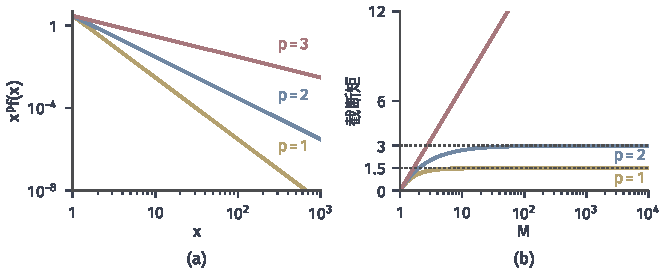
\includegraphics[width=112mm]{figures/07-probability/01-elementary-probability/matplotlib/rvm-moment-existence/figure.pdf}
 \caption{密度$f(x)=3x^{-4}$（$x\geq1$）的矩。(a)双对数坐标下的被积函数$x^{p}f(x)=3x^{p-4}$是直线，斜率为$p-4$；$p=3$时斜率为$-1$，衰减不足以使积分有限。(b)截断矩$\int_1^{M}x^{p}f(x)\,\mathrm{d}x$：$p=1$（黄）与$p=2$（蓝）分别趋于$1.5$与$3$（点线），$p=3$（红）按$3\ln M$增长。}
 \label{fig:rvm-moment-existence}
\end{BookInlineFigure}

离散的例子也一样。第~\ref{sec:rvm-expectation-definition}小节的$p_X(k)=1/[k(k+1)]$满足$k^{p}p_X(k)\leq k^{p-2}$，所以$p<1$时$\mathbb{E}[X^{p}]$有限，而均值是$+\infty$。下表把这些要求的强弱排在一起，每一行的条件蕴含它上面各行的条件。

\begin{BookInlineTable}
 \centering
 \caption{有限矩的要求，以$f(x)=\alpha x^{-\alpha-1}$（$x\geq1$）为例。}
 \label{tab:rvm-moment-requirements}
 \begin{tabular}{lll}
  \toprule
  要求 & 条件 & 使之成立的$\alpha$\\
  \midrule
  均值有限 & $\mathbb{E}\lvert X\rvert<\infty$ & $\alpha>1$\\
  方差有限 & $\mathbb{E}[X^{2}]<\infty$ & $\alpha>2$\\
  偏度有定义 & $\mathbb{E}\lvert X\rvert^{3}<\infty$ & $\alpha>3$\\
  峰度有定义 & $\mathbb{E}[X^{4}]<\infty$ & $\alpha>4$\\
  \bottomrule
 \end{tabular}
\end{BookInlineTable}

\subsection{计算}
\label{sec:rvm-moment-computation}

计算矩就是对幂函数使用函数期望公式，再逐项检查可积性。对密度$2x$，
\[
 m_k=\int_0^1x^{k}\cdot2x\,\mathrm{d}x=\frac{2}{k+2},
\]
于是$m_1=\tfrac23$，$m_2=\tfrac12$，$m_3=\tfrac25$，$m_4=\tfrac13$。直接计算中心矩要展开$(x-\tfrac23)^{k}$再积分，比较繁琐。更好的办法是先算原点矩，再用二项式展开换算。

\begin{theorem}[原点矩与中心矩的换算]
\label{thm:rvm-moment-conversion}
设$k$是正整数，$\mathbb{E}\lvert X\rvert^{k}<\infty$，$\mu=m_1$，并约定$m_0=c_0=1$。则
\begin{align}
 c_k&=\sum_{j=0}^{k}\binom{k}{j}m_j\,(-\mu)^{k-j},
 \label{eq:rvm-central-from-raw}\\
 m_k&=\sum_{j=0}^{k}\binom{k}{j}c_j\,\mu^{k-j}.
 \label{eq:rvm-raw-from-central}
\end{align}
\end{theorem}

\begin{proof}
由定理~\ref{thm:rvm-moment-monotone}，$j\leq k$时$\mathbb{E}\lvert X\rvert^{j}<\infty$，各$m_j$都是有限数。对$(X-\mu)^{k}$用二项式定理，
\[
 (X-\mu)^{k}=\sum_{j=0}^{k}\binom{k}{j}X^{j}(-\mu)^{k-j},
\]
右边是有限个可积变量的线性组合，由线性性逐项取期望得式~\eqref{eq:rvm-central-from-raw}。把$X$写成$(X-\mu)+\mu$再展开，同样得到式~\eqref{eq:rvm-raw-from-central}。
\end{proof}

$k=2$时式~\eqref{eq:rvm-central-from-raw}就是方差展开式$c_2=m_2-\mu^{2}$。$k=3,4$时，代入$m_1=\mu$并合并同类项，得到
\[
 c_3=m_3-3\mu m_2+2\mu^{3},\qquad c_4=m_4-4\mu m_3+6\mu^{2}m_2-3\mu^{4} .
\]

用这两个式子重算奖金表，$\mu=2$。三阶中心矩是
\[
 c_3=45-3\cdot2\cdot9+2\cdot8=7,
\]
与按偏差计算的结果一致。四阶中心矩是
\[
 c_4=243-4\cdot2\cdot45+6\cdot4\cdot9-3\cdot16=243-360+216-48=51 .
\]
对密度$2x$，$\mu=\tfrac23$，代入$m_2=\tfrac12$，$m_3=\tfrac25$，$m_4=\tfrac13$，通分到分母$135$，得到
\[
 c_3=\tfrac25-1+\tfrac{16}{27}=-\tfrac{1}{135},\qquad
 c_4=\tfrac13-\tfrac{16}{15}+\tfrac{4}{3}-\tfrac{16}{27}=\tfrac{1}{135} .
\]
这里$c_4$的四项依次是$m_4$、$4\mu m_3=\tfrac{16}{15}$、$6\mu^{2}m_2=\tfrac43$与$3\mu^{4}=\tfrac{16}{27}$。

\paragraph{平移与缩放}
设$Y=aX+b$。偏差$Y-\mathbb{E}[Y]=a(X-\mu)$与$b$无关，所以中心矩只按缩放变化：
\begin{equation}
 c_k(aX+b)=a^{k}c_k(X),\qquad \mathbb{E}\bigl\lvert Y-\mathbb{E}[Y]\bigr\rvert^{p}=\lvert a\rvert^{p}\,\mathbb{E}\lvert X-\mu\rvert^{p} .
 \label{eq:rvm-central-affine}
\end{equation}
奇数阶中心矩在$a<0$时变号，反映了反射把右侧的偏斜变到左侧。原点矩则随平移改变，$\mathbb{E}[(X+b)^{k}]$按二项式展开是$b$的$k$次多项式。

图~\ref{fig:rvm-raw-central}对奖金表画出了这两种行为。由二项式展开，
\[
 \mathbb{E}[(X+b)^{2}]=9+4b+b^{2},\qquad \mathbb{E}[(X+b)^{3}]=45+27b+6b^{2}+b^{3}
\]
都随$b$变化，而二阶、三阶中心矩始终是$5$与$7$。$b=-\mu=-2$时原点矩与中心矩重合，因为这时$X+b$的均值恰为零。中心矩描述的是质量绕重心的分布，与重心放在数轴何处无关。

\begin{BookInlineFigure}
 \centering
 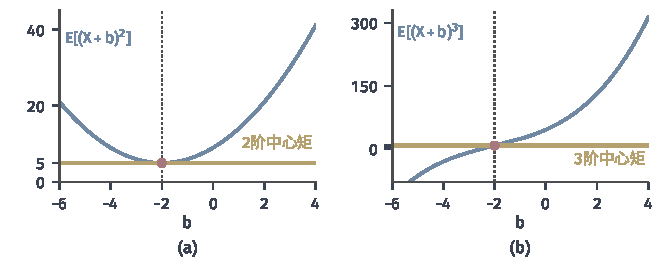
\includegraphics[width=112mm]{figures/07-probability/01-elementary-probability/matplotlib/rvm-raw-central/figure.pdf}
 \caption{平移对原点矩与中心矩的不同影响。对奖金表$X$和平移量$b$：(a)$\mathbb{E}[(X+b)^{2}]$（蓝）是$b$的二次函数，二阶中心矩（黄）恒为$5$；(b)$\mathbb{E}[(X+b)^{3}]$（蓝）是$b$的三次函数，三阶中心矩（黄）恒为$7$。两者在$b=-2$（红点）相交。}
 \label{fig:rvm-raw-central}
\end{BookInlineFigure}

\paragraph{形式展开的陷阱}
换算公式的前提是$\mathbb{E}\lvert X\rvert^{k}<\infty$。缺少这一条时，按形式展开或凭对称性写出的数可能毫无意义。考虑对称的密度
\[
 f_X(x)=\frac{3}{2x^{4}},\qquad \lvert x\rvert\geq1 .
\]
它两侧各有质量$\tfrac12$，均值为$0$，方差是
\[
 \mathbb{E}[X^{2}]=2\int_1^{\infty}x^{2}\cdot\frac{3}{2x^{4}}\,\mathrm{d}x=3\int_1^{\infty}x^{-2}\,\mathrm{d}x=3 .
\]

三阶矩却没有定义：$X^{3}$的正部期望是
\[
 \int_1^{\infty}x^{3}\cdot\frac{3}{2x^{4}}\,\mathrm{d}x=\frac32\int_1^{\infty}\frac{\mathrm{d}x}{x}=+\infty,
\]
负部也是$+\infty$。密度对称会诱使人写下“奇数阶矩为零”，但这只在相应的绝对矩有限时成立，此时被积函数是可积的奇函数。这里$\mathbb{E}\lvert X\rvert^{3}=+\infty$，三阶中心矩和下一小节的偏度都不存在。凡是使用矩的公式，都要先确认它所涉及的最高阶绝对矩有限。

\subsection{偏度与峰度}
\label{sec:rvm-skewness-kurtosis}

三阶中心矩的正负反映偏斜方向，但它的数值带着单位：奖金以元计时$c_3=7$，改用角计时变成$7000$。式~\eqref{eq:rvm-central-affine}说明$c_k$按$a^{k}$缩放，除以$\sigma^{k}$就消去了尺度。等价地，先标准化再求矩。

\begin{definition}[偏度与峰度]
\label{def:rvm-skewness-kurtosis}
设$0<\operatorname{Var}(X)=\sigma^{2}<\infty$，$\mu=\mathbb{E}[X]$，$Z=(X-\mu)/\sigma$。若$\mathbb{E}\lvert X\rvert^{3}<\infty$，称
\begin{equation}
 \gamma_1=\frac{c_3}{\sigma^{3}}=\mathbb{E}[Z^{3}]
 \label{eq:rvm-skewness}
\end{equation}
为$X$的\term{偏度}（skewness）。若$\mathbb{E}[X^{4}]<\infty$，称
\begin{equation}
 \kappa=\frac{c_4}{\sigma^{4}}=\mathbb{E}[Z^{4}]
 \label{eq:rvm-kurtosis}
\end{equation}
为$X$的\term{峰度}（kurtosis），称$\kappa-3$为\term{超额峰度}（excess kurtosis）。
\end{definition}

由式~\eqref{eq:rvm-central-affine}，对$a>0$，$aX+b$与$X$的偏度和峰度都相同；对$a<0$，偏度变号，峰度不变。超额峰度减去的$3$，是下一章将要介绍的高斯分布的峰度。不同文献对“峰度”一词有时指$\kappa$、有时指$\kappa-3$，读数之前要先确认约定。这里讨论的是给定分布的总体量；由观测数据估计偏度和峰度属于统计推断。

两个贯穿例子的值如下。奖金表的
\[
 \gamma_1=\frac{7}{5^{3/2}}\approx0.626,\qquad \kappa=\frac{51}{25}=2.04 .
\]
密度$2x$的方差是$\tfrac{1}{18}$，$\sigma^{3}=1/(54\sqrt2)$，$\sigma^{4}=\tfrac{1}{324}$，于是
\[
 \gamma_1=-\frac{54\sqrt2}{135}=-\frac{2\sqrt2}{5}\approx-0.566,\qquad \kappa=\frac{324}{135}=\frac{12}{5} .
\]
奖金表的偏度为正：远处那个$6$元在均值右侧，立方把它的影响放大。密度$2x$的质量堆在右端，左侧有一条渐渐变薄的长边，偏度为负。

\paragraph{零偏度不保证对称}
若$X$关于$\mu$对称且$\mathbb{E}\lvert X\rvert^{3}<\infty$，则$(X-\mu)^{3}$与$-(X-\mu)^{3}$同分布，$c_3=-c_3$，偏度为零。反过来不成立。设$Y$以概率$\tfrac16,\tfrac12,\tfrac13$取$-5,-1,4$。它的均值和三阶矩分别是
\[
 \mathbb{E}[Y]=-\tfrac56-\tfrac12+\tfrac43=0,\qquad
 \mathbb{E}[Y^{3}]=-\tfrac{125}{6}-\tfrac12+\tfrac{64}{3}=0 .
\]
所以$c_3=0$，偏度为零。但$Y$不对称：取负值的概率是$\tfrac23$，中位数是$-1$而不是均值$0$。图~\ref{fig:rvm-zero-skew}显示，零偏度只是左侧一个远偏差的立方与右侧一个中等偏差的立方恰好抵消。

\begin{BookInlineFigure}
 \centering
 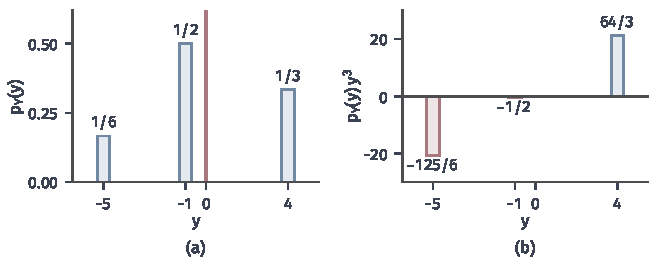
\includegraphics[width=112mm]{figures/07-probability/01-elementary-probability/matplotlib/rvm-zero-skew/figure.pdf}
 \caption{偏度为零的不对称分布。(a)$Y$以概率$\tfrac16,\tfrac12,\tfrac13$取$-5,-1,4$，均值为$0$（红线），方差为$10$。(b)三阶矩的各项贡献$p_Y(y)\,y^{3}$：左侧两项（红）之和$-\tfrac{64}{3}$与右侧一项（蓝）$\tfrac{64}{3}$相互抵消。}
 \label{fig:rvm-zero-skew}
\end{BookInlineFigure}

\paragraph{峰度衡量什么}
由标准化变量$Z$的$\mathbb{E}[Z^{2}]=1$，可以把峰度改写成
\[
 \kappa-1=\mathbb{E}[Z^{4}]-\bigl(\mathbb{E}[Z^{2}]\bigr)^{2}=\operatorname{Var}(Z^{2}) .
\]
这给出了峰度的一个准确读法：它衡量$Z^{2}$在其均值$1$周围的波动。若质量都集中在$\lvert Z\rvert=1$附近，$Z^{2}$几乎不变，峰度接近$1$；若一部分质量在中心附近、另一部分在很远处，$Z^{2}$变化剧烈，峰度就大。所以峰度同时受中心附近和远处的影响，不能只理解为峰的尖锐程度。由这个读法还可以得到峰度与偏度之间的约束。

\begin{theorem}[偏度与峰度的约束]
\label{thm:rvm-pearson}
设$\mathbb{E}[X^{4}]<\infty$且$\operatorname{Var}(X)>0$。则
\begin{equation}
 \kappa\geq1+\gamma_1^{2} .
 \label{eq:rvm-pearson}
\end{equation}
对离散的$X$，等号成立当且仅当$X$以概率一只取两个值。
\end{theorem}

\begin{proof}
记$Z$为标准化变量，考虑非负变量$W=(Z^{2}-\gamma_1Z-1)^{2}$。展开后各项都是$Z$的不超过四次的幂，都可积：
\[
 W=Z^{4}-2\gamma_1Z^{3}+(\gamma_1^{2}-2)Z^{2}+2\gamma_1Z+1 .
\]
代入$\mathbb{E}[Z]=0$，$\mathbb{E}[Z^{2}]=1$，$\mathbb{E}[Z^{3}]=\gamma_1$，$\mathbb{E}[Z^{4}]=\kappa$，由线性性得
\[
 0\leq\mathbb{E}[W]=\kappa-2\gamma_1^{2}+\gamma_1^{2}-2+1=\kappa-\gamma_1^{2}-1 .
\]

等号成立当且仅当$\mathbb{E}[W]=0$。对离散的$X$，这等价于$Z$的每个正概率取值都是二次方程$z^{2}-\gamma_1z-1=0$的根。这个方程的判别式$\gamma_1^{2}+4>0$，恰有两个实根，所以$Z$至多取两个值；它的方差为一，不是常数，因此恰好取两个值。反过来，设$Z$只取两个值$z_1<z_2$，概率分别为$1-r$与$r$。由$\mathbb{E}[Z]=0$得$(1-r)z_1=-rz_2$，代入$\mathbb{E}[Z^{2}]=1$，
\[
 1=(1-r)z_1\cdot z_1+rz_2\cdot z_2=-rz_2z_1-(1-r)z_1z_2=-z_1z_2 .
\]
所以$z_1,z_2$是二次方程$z^{2}-(z_1+z_2)z-1=0$的两个根，于是
\[
 z_k^{2}=(z_1+z_2)z_k+1,\qquad k=1,2 .
\]两边乘$z_k$后取期望，得到
\[
 \gamma_1=\mathbb{E}[Z^{3}]=(z_1+z_2)\,\mathbb{E}[Z^{2}]+\mathbb{E}[Z]=z_1+z_2 .
\]于是$Z$的两个取值都满足$z^{2}-\gamma_1z-1=0$，$W$恒为零，等号成立。
\end{proof}

图~\ref{fig:rvm-skew-kurt-plane}把本节的例子放到偏度—峰度平面上。抛物线$\kappa=1+\gamma_1^{2}$下方的区域不可能出现；两点分布恰好落在抛物线上，例如以概率$\tfrac56,\tfrac16$取$1,7$的表，偏度$4/\sqrt5\approx1.79$，峰度$4.2$。三点或更多点的分布与有密度的分布都在抛物线上方。

\begin{BookInlineFigure}
 \centering
 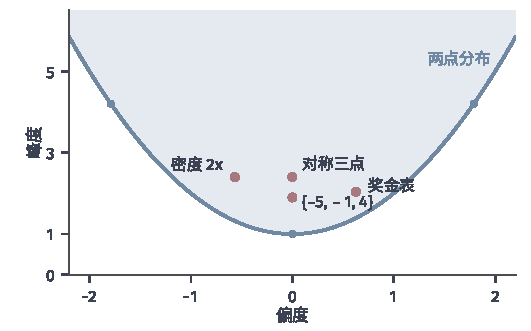
\includegraphics[width=90mm]{figures/07-probability/01-elementary-probability/matplotlib/rvm-skew-kurt-plane/figure.pdf}
 \caption{偏度—峰度平面。可能出现的点位于抛物线$\kappa=1+\gamma_1^{2}$上或其上方（浅蓝区域），两点分布落在抛物线上（蓝点为取值概率$\tfrac16,\tfrac12,\tfrac56$的三例）。红点是本节的例子：奖金表$(0.63,2.04)$，密度$2x$为$(-0.57,2.4)$，$Y$在$\{-5,-1,4\}$上为$(0,1.9)$，对称三点分布为$(0,2.4)$。}
 \label{fig:rvm-skew-kurt-plane}
\end{BookInlineFigure}

\paragraph{峰度不能单独确定形状}
同一个峰度可以对应形状完全不同的分布。设$Z$以概率$q,1-2q,q$取$-a,0,a$。方差为一要求$2qa^{2}=1$，而$\mathbb{E}[Z^{4}]=2qa^{4}=\frac{1}{2q}$。取$q=\tfrac{5}{24}$，峰度是$\tfrac{12}{5}$，与密度$2x$的峰度相同。

图~\ref{fig:rvm-same-kurtosis}把两者并列：一个是向右上升、支撑有界、偏度为负的三角形密度，另一个是对称的三点分布，中间有一个高的质量。两者峰度都是$2.4$，低于$3$。峰度既不能说明峰的尖锐，也不能说明尾部是否有界，它只是$Z^{2}$的波动这一个数。描述尾部的衰减规律要直接看尾概率，第~\ref{chap:tail-probabilities}章会用矩来估计它。

\begin{BookInlineFigure}
 \centering
 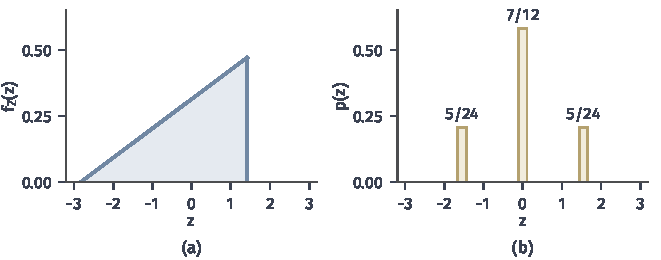
\includegraphics[width=112mm]{figures/07-probability/01-elementary-probability/matplotlib/rvm-same-kurtosis/figure.pdf}
 \caption{峰度相同而形状不同的两个标准化分布。(a)密度$2x$标准化后的三角形密度（蓝），偏度$-0.57$；(b)以概率$\tfrac{5}{24},\tfrac{7}{12},\tfrac{5}{24}$取$-1.55,0,1.55$的对称三点分布（黄），偏度$0$。两者均值为$0$、方差为$1$，峰度都是$12/5$。}
 \label{fig:rvm-same-kurtosis}
\end{BookInlineFigure}

\subsection{矩对分布的刻画}
\label{sec:rvm-moments-characterize}

均值、方差、偏度、峰度一个比一个记录更细的信息。自然要问：知道前几个矩，能否确定分布？如果能，概率表与密度就可以用一串数代替。答案是否定的，而且相差得很远。

\paragraph{均值与方差相同的三张表}
奖金表的均值是$2$，方差是$5$。两点分布的方差有一个简单公式：以概率$1-r$与$r$取$a<b$时，均值$\mu$满足$(1-r)(a-\mu)+r(b-\mu)=0$，方差等于$(b-\mu)(\mu-a)$。要求$\mu=2$、方差为$5$，可取$a=1,b=7$，此时$r=\tfrac16$；也可取$a=-3,b=3$，此时$r=\tfrac56$。

于是三张表以概率$\tfrac12,\tfrac13,\tfrac16$取$0,3,6$，以概率$\tfrac56,\tfrac16$取$1,7$，以概率$\tfrac16,\tfrac56$取$-3,3$，它们的均值都是$2$、方差都是$5$。图~\ref{fig:rvm-same-mean-var}显示它们的形状截然不同：第二张右偏，第三张左偏，偏度分别为$\pm4/\sqrt5\approx\pm1.79$，奖金表的偏度是$0.63$。均值和方差只确定了重心与转动惯量，质量怎样具体分配，它们管不到。

\begin{BookInlineFigure}
 \centering
 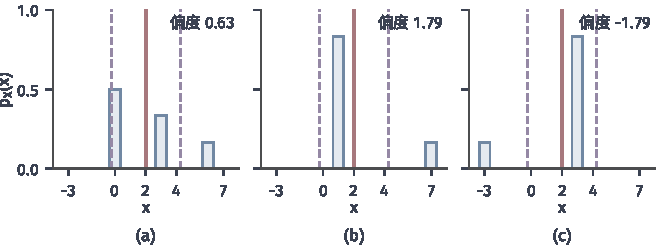
\includegraphics[width=112mm]{figures/07-probability/01-elementary-probability/matplotlib/rvm-same-mean-var/figure.pdf}
 \caption{均值都是$2$（红线）、方差都是$5$的三张概率表，紫色虚线是均值加减标准差$\sqrt5$。(a)奖金表；(b)以概率$\tfrac56,\tfrac16$取$1,7$；(c)以概率$\tfrac16,\tfrac56$取$-3,3$。三者的偏度分别为$0.63$、$1.79$与$-1.79$。}
 \label{fig:rvm-same-mean-var}
\end{BookInlineFigure}

\paragraph{有限个矩不能确定分布}
增加矩的个数也无济于事。只要多给出几个矩，就能用更细的扰动保持它们不变，下面的定理把这一点做成构造。

\begin{theorem}[有限个矩不确定分布]
\label{thm:rvm-finite-moments}
对每个正整数$k$，存在$(0,1)$上的密度$f\neq1$，使以$f$为密度的变量与以常数$1$为密度的变量具有相同的$1,\dots,k$阶矩，而$k+1$阶矩不同。
\end{theorem}

\begin{proof}
寻找次数不超过$k+1$的多项式$q(x)=\sum_{l=0}^{k+1}a_lx^{l}$，使
\begin{equation}
 \int_0^1x^{j}q(x)\,\mathrm{d}x=0,\qquad j=0,1,\dots,k .
 \label{eq:rvm-orthogonal}
\end{equation}
这是关于$k+2$个系数$a_0,\dots,a_{k+1}$的$k+1$个齐次线性方程，未知数多于方程，所以有非零解。非零多项式在$[0,1]$上不恒为零，记$M=\max_{[0,1]}\lvert q\rvert>0$，把$q$换成$q/M$，就可设$\max_{[0,1]}\lvert q\rvert=1$。

令$f=1+q$。它在$(0,1)$上非负，由式~\eqref{eq:rvm-orthogonal}中$j=0$的方程，总积分为一，所以是密度；它不恒等于$1$。对$1\leq j\leq k$，
\[
 \int_0^1x^{j}f(x)\,\mathrm{d}x=\int_0^1x^{j}\,\mathrm{d}x+\int_0^1x^{j}q(x)\,\mathrm{d}x=\int_0^1x^{j}\,\mathrm{d}x,
\]
前$k$阶矩相同。若$k+1$阶矩也相同，则$q$与$1,x,\dots,x^{k+1}$的乘积积分都为零，从而与自身的乘积积分$\int_0^1q^{2}\,\mathrm{d}x=0$，这对非零多项式不可能。
\end{proof}

$k=2$时可以取$q(x)=20x^{3}-30x^{2}+12x-1$。逐项积分可以核对式~\eqref{eq:rvm-orthogonal}：
\[
 \begin{aligned}
 \int_0^1q(x)\,\mathrm{d}x&=5-10+6-1=0,\\
 \int_0^1xq(x)\,\mathrm{d}x&=4-\tfrac{15}{2}+4-\tfrac12=0,\\
 \int_0^1x^{2}q(x)\,\mathrm{d}x&=\tfrac{10}{3}-6+3-\tfrac13=0 .
 \end{aligned}
\]
它在$[0,1]$上的最大绝对值是$1$，在两个端点取到。于是$f=1+q$与常数密度有相同的均值$\tfrac12$和方差$\tfrac1{12}$，三阶矩则多出$\int_0^1x^{3}q\,\mathrm{d}x=\tfrac{1}{140}$。$k=4$时类似地取一个五次多项式。图~\ref{fig:rvm-same-moments}显示，保持的矩越多，扰动的波动越多，但两个密度始终明显不同。

\begin{BookInlineFigure}
 \centering
 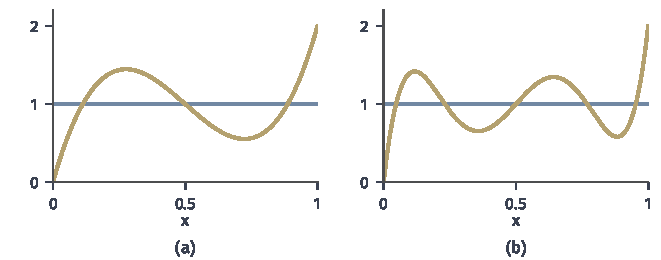
\includegraphics[width=112mm]{figures/07-probability/01-elementary-probability/matplotlib/rvm-same-moments/figure.pdf}
 \caption{前几个矩相同的不同密度。(a)常数密度$1$（蓝）与$1+q(x)$（黄），$q(x)=20x^{3}-30x^{2}+12x-1$，两者的前两阶矩相同；(b)常数密度与$1+252x^{5}-630x^{4}+560x^{3}-210x^{2}+30x-1$，前四阶矩相同。保持的矩越多，扰动振荡越快。}
 \label{fig:rvm-same-moments}
\end{BookInlineFigure}

那么全部矩能否确定分布？结论取决于尾部的轻重。取值有界时，全部矩确实决定分布，证明要用多项式在有界区间上一致逼近连续函数。尾部较重时则不然：存在各阶矩都有限且全部相同的两个不同分布，构造它们要用到第~\ref{chap:random-variable-transformations}章的密度换元，相关讨论可查阅~\scite{math-kallenberg2021probability}。用变换判断两个分布是否相同的系统工具在第~\ref{chap:weak-convergence-of-distributions}章介绍。在那之前，矩应当被看作分布的数值概括：它们回答特定的问题，例如平均、波动、偏斜，但不能代替概率表、分布函数或密度。


\section{本章小结}
\label{sec:rvm-summary}

本章从一张概率表出发，问怎样用少数几个数概括它。期望是概率质量的重心，按概率加权平均取值；方差是绕重心的转动惯量，按概率加权平均偏差的平方；更高阶的矩加重远处偏差的权重，标准化后的三阶、四阶矩描述偏斜方向与$Z^{2}$的波动。奖金表与密度$2x$贯穿全章，表~\ref{tab:rvm-summary}汇总了它们的各项数值。

\begin{BookInlineTable}
 \centering
 \caption{两个贯穿例子的数值特征。}
 \label{tab:rvm-summary}
 \begin{tabular}{lcc}
  \toprule
  数值特征 & 奖金表 & 密度$2x$\\
  \midrule
  均值$\mu$ & $2$ & $2/3$\\
  方差$\sigma^{2}$ & $5$ & $1/18$\\
  标准差$\sigma$ & $2.24$ & $0.236$\\
  三阶中心矩$c_3$ & $7$ & $-1/135$\\
  四阶中心矩$c_4$ & $51$ & $1/135$\\
  偏度$\gamma_1$ & $0.626$ & $-0.566$\\
  峰度$\kappa$ & $2.04$ & $2.4$\\
  \bottomrule
 \end{tabular}
\end{BookInlineTable}

每个数回答一个特定的问题，也需要特定的条件，表~\ref{tab:rvm-summary-roles}把它们与第~\ref{chap:random-variables}章的分位数放在一起比较。均值与中位数都描述位置，前者使平方误差最小、受远处取值牵动，后者使绝对误差最小、只看左右质量的分配。方差与标准差描述波动尺度，标准差与变量同单位。偏度与峰度不随单位改变，却只是两个数，零偏度不保证对称，峰度也不能确定峰形或尾部规律。

\begin{BookInlineTable}
 \centering
 \caption{各数值特征回答的问题、存在条件与在$aX+b$（$a\neq0$）下的变化。偏度与峰度还要求$\sigma>0$。}
 \label{tab:rvm-summary-roles}
 \begin{tabular}{llll}
  \toprule
  特征 & 回答的问题 & 存在条件 & 在$aX+b$下\\
  \midrule
  均值 & 重心在哪里 & $\mathbb{E}\lvert X\rvert<\infty$ & $a\mu+b$\\
  中位数 & 左右各半的位置 & 总存在 & 随之变换\\
  方差 & 绕重心散开多少 & $\mathbb{E}[X^{2}]<\infty$ & $a^{2}\sigma^{2}$\\
  标准差 & 同单位的波动 & $\mathbb{E}[X^{2}]<\infty$ & $\lvert a\rvert\sigma$\\
  $k$阶中心矩 & 偏差的$k$次平均 & $\mathbb{E}\lvert X\rvert^{k}<\infty$ & $a^{k}c_k$\\
  偏度 & 偏斜方向 & $\mathbb{E}\lvert X\rvert^{3}<\infty$ & $a<0$时变号\\
  峰度 & $Z^{2}$的波动 & $\mathbb{E}[X^{4}]<\infty$ & 不变\\
  \bottomrule
 \end{tabular}
\end{BookInlineTable}

存在条件是使用这些数的前提。非负变量的期望总有意义但可能为$+\infty$；有符号变量要分别检查正部与负部，两者都无穷时期望不存在，对称也不能补救。高阶绝对矩有限蕴含低阶绝对矩有限，Lyapunov不等式给出了定量的比较；反方向不成立，幂律尾部的密度$\alpha x^{-\alpha-1}$只有低于$\alpha$阶的矩。一切展开公式和对称性论证都要先确认所涉最高阶的绝对矩有限。

运算规则同样有边界。期望的线性性对可积变量的有限线性组合成立，不需要独立性，信封问题说明它能绕开复杂的依赖结构。乘积的期望一般不能拆开，无穷求和与取期望的交换需要额外条件。函数的期望可以直接用原变量的分布计算，不必求出新变量的分布，但要对每个函数检查绝对可积。凸函数满足Jensen不等式，变量越分散，“先平均再变换”与“先变换再平均”相差越大。方差的展开式便于手算，数值计算中则应先减去均值。

数值特征是分布的概括，不是替代。均值和方差相同的概率表形状可以完全不同；对任意给定的$k$，都有前$k$阶矩相同的不同密度。尾概率的估计、和的方差以及用变换识别分布，分别在第~\ref{chap:tail-probabilities}章、第~\ref{chap:random-vectors}章与第~\ref{chap:weak-convergence-of-distributions}章展开。下一章把本章的工具用于常见分布，在每个模型的试验机制和参数下计算均值与方差，并检查它们是否存在。


\chapter{常见分布}
\label{chap:common-distributions}

一条生产线上，每个零件是次品的概率是$0.2$。质检员可以用好几种方式记录结果：抽查一个零件，看它是不是次品；连续检查$10$个零件，数其中的次品；从一箱$20$个、其中恰有$4$个次品的零件里不放回地取出$10$个，数其中的次品；或者一个一个往下查，直到遇到第一个次品为止。这四种记录都取非负整数，前三种的平均值都是$2$，可它们的概率规律各不相同。

连续取值的记录也是如此。等待下一次故障的时间只取正值，零件长度的测量误差可正可负，一批货中次品所占的比例落在$0$与$1$之间。前两章已经准备好了描述分布的工具（分布函数、概率质量与密度）和概括分布的数值（期望、方差与矩）。现在要问的是：给定一种试验机制或一种取值范围，概率规律应当是什么样子，它的参数各管什么，期望和方差等于多少，又是否存在。

离散部分从一次成败出发，依次加入固定次数的独立重复、有限总体的不放回抽样、等待首次成功和稀有事件的计数，每个模型都由试验机制推出质量函数。连续部分从区间上的均匀取值开始，经过等待时间和测量误差，再到正值变量、比例和带有大偏差的波动；每个模型先核对密度的归一化，再计算期望与方差，并记下矩不存在的情形。

最后把这些模型并排比较，说明为什么不能只凭均值相同就互相替代。第~\ref{chap:tail-probabilities}章用这里的模型检验尾概率的上界，第~\ref{chap:multivariate-distributions}章和第~\ref{chap:random-variable-transformations}章则以这里的一元模型为构件。

\section{离散分布}
\label{sec:cdist-discrete}

离散模型的取值可以一个一个列出来，概率由质量函数给出。建立这样的模型有固定的步骤：先说清基本试验是什么，各次试验之间有没有牵连，随机变量记录的又是什么；再用计数和第~\ref{chap:classical-probability}章的乘法规则推出质量函数，核对它非负、总和为一；最后计算期望和方差。

参数的名字相近，并不说明试验机制相同。二项分布和几何分布都有一个“成功概率$p$”，但前者固定试验次数、数成功的个数，后者固定只等一次成功、数试验的次数。二项分布和超几何分布都有一个“抽取个数$n$”，但前者各次互不影响，后者每抽走一个都会改变剩下的构成。下面五个模型都用开头那条生产线演示，便于比较。

\subsection{Bernoulli分布}
\label{sec:cdist-bernoulli}

最简单的随机记录只有两种结果：零件是次品或不是，硬币是正面或反面。把关心的那种结果叫作“成功”，记为$1$，另一种记为$0$，就得到只取两个值的随机变量。它的分布只需要一个数来描述。

\begin{definition}[Bernoulli分布]
\label{def:cdist-bernoulli}
设$0\leq p\leq1$。若随机变量$X$只取$0,1$两个值，且
\begin{equation}
  \mathbb{P}(X=1)=p,\qquad \mathbb{P}(X=0)=1-p,
  \label{eq:cdist-bernoulli-pmf}
\end{equation}
则称$X$服从参数为$p$的\term{Bernoulli分布}（Bernoulli distribution），记作$X\sim\operatorname{Bern}(p)$，$p$称为成功概率。
\end{definition}

两个概率也可以合写成一个质量函数$p_X(x)=p^{x}(1-p)^{1-x}$，$x\in\{0,1\}$。这里约定$0^{0}=1$，这样$p=0$或$p=1$时公式仍然成立。

期望按概率加权平均计算：
\[
  \mathbb{E}[X]=0\cdot(1-p)+1\cdot p=p .
\]
$X$只取$0$和$1$，所以$X^{2}=X$，于是$\mathbb{E}[X^{2}]=p$。代入第~\ref{chap:random-variable-moments}章的方差展开式，即二阶矩减去期望的平方，得到
\begin{equation}
  \mathbb{E}[X]=p,\qquad \operatorname{Var}(X)=p(1-p).
  \label{eq:cdist-bernoulli-moments}
\end{equation}

把概率看成质量，就能看出这两个数的含义。点$0$上放质量$1-p$，点$1$上放质量$p$，重心落在$p$处，这就是期望；生产线的例子中$p=0.2$，期望$0.2$并不是$X$能取到的值。方差是质量相对重心的转动惯量，两端质量相等时最大，在$p=1/2$处达到$1/4$；例中方差为$0.16$。图~\ref{fig:cdist-bernoulli-variance}画出了这两点。

\begin{BookInlineFigure}
  \centering
  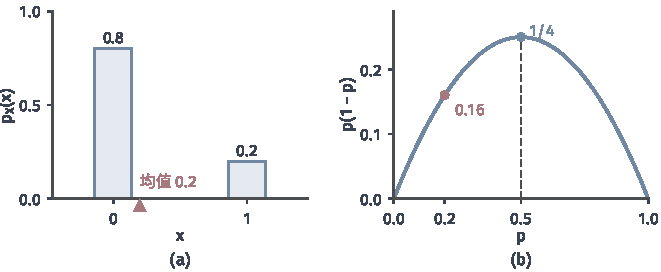
\includegraphics[width=112mm]{figures/07-probability/01-elementary-probability/matplotlib/cdist-bernoulli-variance/figure.pdf}
  \caption{Bernoulli分布。(a)$p=0.2$的质量表，红色三角是期望$0.2$，也就是两根柱子的重心。(b)方差$p(1-p)$随$p$的变化，蓝点为最大值$1/4$（$p=1/2$），红点为例中的$0.16$。}
  \label{fig:cdist-bernoulli-variance}
\end{BookInlineFigure}

端点$p=0$和$p=1$也算Bernoulli分布，但这时$X$以概率一取固定值，方差为零，与第~\ref{chap:random-variable-moments}章“方差为零即以概率一取常数”的结论一致。后面的模型在参数取到端点时也会出现这种退化，届时都要单独核对。

\paragraph{指示变量}
任何事件都可以用一个Bernoulli变量来记录。对事件$A$，令
\begin{equation}
  \mathbf{1}_{A}(\omega)=
  \begin{cases}
    1, & \omega\in A,\\
    0, & \omega\notin A,
  \end{cases}
  \label{eq:cdist-indicator}
\end{equation}
称为$A$的\term{指示变量}（indicator variable）。它在$A$发生时取$1$，否则取$0$，所以$\mathbf{1}_{A}\sim\operatorname{Bern}(\mathbb{P}(A))$，并且
\begin{equation}
  \mathbb{E}[\mathbf{1}_{A}]=\mathbb{P}(A).
  \label{eq:cdist-indicator-mean}
\end{equation}

图~\ref{fig:cdist-indicator}以掷两枚骰子为例。样本空间有$36$个等可能的点，事件$A$为“点数之和不小于$10$”，含$6$个点。指示变量把这$6$个点送到$1$，其余$30$个点送到$0$，得到的质量表是$5/6$与$1/6$，期望正是$\mathbb{P}(A)=1/6$。

\begin{BookInlineFigure}
  \centering
  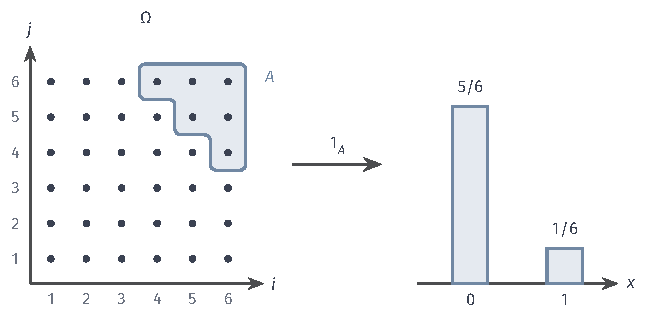
\includegraphics[width=109mm]{figures/07-probability/01-elementary-probability/tikz/cdist-indicator/figure.pdf}
  \caption{指示变量是样本空间上的函数。左：两枚骰子的$36$个样本点，浅蓝区域是事件$A=\{i+j\geq10\}$。右：$\mathbf{1}_{A}$的质量表，$A$中的$6$个点贡献点$1$上的质量$1/6$。}
  \label{fig:cdist-indicator}
\end{BookInlineFigure}

指示变量还有两条代数性质，下面两小节要反复使用。第一条是$\mathbf{1}_{A}^{2}=\mathbf{1}_{A}$，因为$0^{2}=0$、$1^{2}=1$。第二条是乘积等于交事件的指示变量：
\begin{equation}
  \mathbf{1}_{A}\mathbf{1}_{B}=\mathbf{1}_{A\cap B},
  \label{eq:cdist-indicator-product}
\end{equation}
因为两边都在$A$与$B$同时发生时取$1$，否则取$0$。

有了这两条，“$n$个事件中发生了几个”就能写成$\mathbf{1}_{A_1}+\dots+\mathbf{1}_{A_n}$。由期望的线性性和式~\eqref{eq:cdist-indicator-mean}，它的期望等于$\mathbb{P}(A_1)+\dots+\mathbb{P}(A_n)$，这一步对事件之间的任何牵连都成立。计数问题因此可以拆成单个事件的概率来算。

\subsection{二项分布}
\label{sec:cdist-binomial}

连续检查$10$个零件，次品数$X$可能取$0,1,\dots,10$中的任何一个。要写出$\mathbb{P}(X=k)$，先把假设说清楚：每个零件是次品的概率都是$0.2$，而且各零件是否为次品互不影响。

一般地，进行$n$次试验，记$A_i$为“第$i$次成功”，并假设三条：试验次数$n$事先固定；每次成功的概率都是$p$；事件$A_1,\dots,A_n$相互独立。成功的总次数是$n$个指示变量之和，
\[
  X=\mathbf{1}_{A_1}+\mathbf{1}_{A_2}+\dots+\mathbf{1}_{A_n}.
\]

\paragraph{质量函数}
$X=k$意味着恰好有$k$个$A_i$发生。先固定一组成功的位置$S\subseteq\{1,\dots,n\}$，$\lvert S\rvert=k$，考虑事件“$i\in S$时$A_i$发生，$i\notin S$时$A_i$不发生”。相互独立的事件把其中一部分换成补事件后仍然相互独立（第~\ref{chap:classical-probability}章），所以这个事件的概率是$k$个$p$与$n-k$个$1-p$之积：
\[
  p^{k}(1-p)^{n-k}.
\]
这个值只依赖于成功的个数，与成功出现在哪些位置无关。

从$n$个位置中选出$k$个作为成功位置，共有$\binom{n}{k}$种选法，可参考\BookChapterRef{chap:counting}{卷一第2章“计数”}。不同的$S$对应的事件互不相容，把它们的概率加起来，就得到$X$的质量函数。

\begin{definition}[二项分布]
\label{def:cdist-binomial}
设$n$为正整数，$0\leq p\leq1$。若随机变量$X$的质量函数为
\begin{equation}
  \mathbb{P}(X=k)=\binom{n}{k}p^{k}(1-p)^{n-k},\qquad k=0,1,\dots,n,
  \label{eq:cdist-binomial-pmf}
\end{equation}
则称$X$服从参数为$n,p$的\term{二项分布}（binomial distribution），记作$X\sim\operatorname{Bin}(n,p)$。
\end{definition}

由二项式定理，质量函数的总和是$(p+(1-p))^{n}=1$，名字也由此而来。$n=1$时它就是$\operatorname{Bern}(p)$。

图~\ref{fig:cdist-binomial-sequences}把$n=3$、$p=0.2$的八种结果按成功次数分成四组。每一条结果的概率只看其中有几个成功，同组各条相同；组内条数是$\binom{3}{k}$，乘起来就是$\mathbb{P}(X=k)$。

\begin{BookInlineFigure}
  \centering
  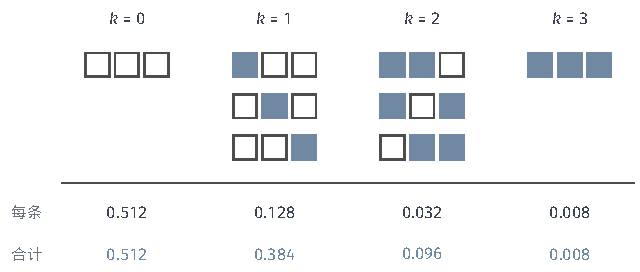
\includegraphics[width=108mm]{figures/07-probability/01-elementary-probability/tikz/cdist-binomial-sequences/figure.pdf}
  \caption{$n=3$次独立试验、$p=0.2$时的八种结果，蓝色方格表示成功。按成功次数$k$分组：每条结果的概率为$p^{k}(1-p)^{3-k}$，组内共$\binom{3}{k}$条，合计即二项概率，四个合计之和为$1$。}
  \label{fig:cdist-binomial-sequences}
\end{BookInlineFigure}

回到$n=10$、$p=0.2$的检查。由式~\eqref{eq:cdist-binomial-pmf}，没有次品和恰有两个次品的概率分别是
\[
  \mathbb{P}(X=0)=0.8^{10}\approx0.1074,\qquad
  \mathbb{P}(X=2)=45\times0.2^{2}\times0.8^{8}\approx0.3020 .
\]
次品不少于$4$个的概率为$1-\mathbb{P}(X\leq3)\approx0.1209$。

\paragraph{形状}
设$0<p<1$，质量函数先升后降。相邻两项之比为
\[
  \frac{\mathbb{P}(X=k+1)}{\mathbb{P}(X=k)}=\frac{(n-k)p}{(k+1)(1-p)},
\]
它大于$1$当且仅当$(n-k)p>(k+1)(1-p)$，整理后即$k<(n+1)p-1$。所以概率在$k$小于$(n+1)p-1$时上升，之后下降，最大值落在$\lfloor(n+1)p\rfloor$处；$(n+1)p$恰为整数时，它和前一个整数并列最大。例中$(n+1)p=2.2$，最可能的次品数是$2$。

把成功与失败对调，$k$次成功就是$n-k$次失败，所以$\operatorname{Bin}(n,1-p)$的质量函数是$\operatorname{Bin}(n,p)$的左右翻转。图~\ref{fig:cdist-binomial-pmf}(b)中$p=0.8$的柱子正是图~\ref{fig:cdist-binomial-pmf}(a)的镜像，$p=0.5$时左右对称。

\begin{BookInlineFigure}
  \centering
  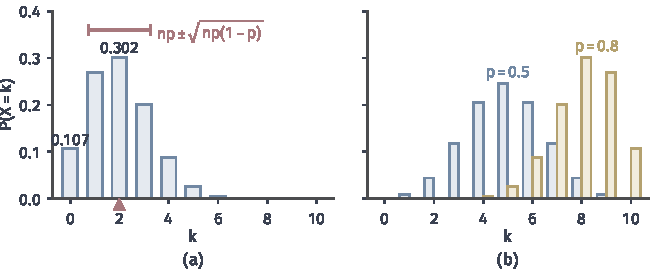
\includegraphics[width=112mm]{figures/07-probability/01-elementary-probability/matplotlib/cdist-binomial-pmf/figure.pdf}
  \caption{二项分布的质量函数，$n=10$。(a)$p=0.2$，红色三角为期望$2$，红色横线标出期望左右各一个标准差$\sqrt{1.6}\approx1.26$的范围。(b)$p=0.5$（蓝）和$p=0.8$（黄），后者是(a)的左右翻转。}
  \label{fig:cdist-binomial-pmf}
\end{BookInlineFigure}

\paragraph{期望与方差}
期望直接由指示变量之和得到。由线性性和式~\eqref{eq:cdist-indicator-mean}，
\[
  \mathbb{E}[X]=\sum_{i=1}^{n}\mathbb{P}(A_i)=np .
\]
这一步没有用到独立性。

方差要先算$\mathbb{E}[X^{2}]$。把平方展开成双重和，并把$i=j$与$i\neq j$的项分开：
\[
  X^{2}=\sum_{i=1}^{n}\sum_{j=1}^{n}\mathbf{1}_{A_i}\mathbf{1}_{A_j}
  =\sum_{i=1}^{n}\mathbf{1}_{A_i}+\sum_{i\neq j}\mathbf{1}_{A_i\cap A_j},
\]
这里用了$\mathbf{1}_{A_i}^{2}=\mathbf{1}_{A_i}$和式~\eqref{eq:cdist-indicator-product}。第二个和共有$n(n-1)$个有序对$(i,j)$。

对两边取期望。由独立性，$i\neq j$时$\mathbb{P}(A_i\cap A_j)=p^{2}$，于是
\[
  \mathbb{E}[X^{2}]=np+n(n-1)p^{2}.
\]
再减去期望的平方，
\[
  \operatorname{Var}(X)=np+n(n-1)p^{2}-n^{2}p^{2}=np-np^{2}.
\]
合起来就是
\begin{equation}
  \mathbb{E}[X]=np,\qquad \operatorname{Var}(X)=np(1-p).
  \label{eq:cdist-binomial-moments}
\end{equation}
例中期望为$2$，方差为$1.6$，标准差约$1.26$。

\paragraph{三个量的区分}
二项模型里有三个量，含义各不相同。试验次数$n$是事先设计好的，成功概率$p$是模型的参数，$X$则是试验做完才看到的计数。看到$X=3$并不等于知道$p=0.3$，由观察到的计数反推$p$属于统计推断，可参考\BookChapterRef{chap:parametric-statistical-inference}{卷八第1章“参数化统计推断”}。

\paragraph{去掉条件会怎样}
三条假设少了任何一条，式~\eqref{eq:cdist-binomial-pmf}都不再成立。先看成功概率不相同的情形：两次试验相互独立，第一次必然失败，第二次必然成功。成功次数恒为$1$，方差为零；平均成功概率同样是$1/2$的$\operatorname{Bin}(2,1/2)$却有方差$1/2$。

再看独立性。假设$10$个零件出自同一副模具，要么全是次品，要么全是合格品，前者的概率为$0.2$。此时每个零件仍以$0.2$的概率是次品，次品数只取$0$和$10$，期望仍是$2$。可方差变成了
\[
  \mathbb{E}[X^{2}]-(\mathbb{E}[X])^{2}=0.2\times100-4=16,
\]
是二项模型的十倍。期望的计算不需要独立性，方差却完全取决于事件之间的牵连。

\subsection{超几何分布}
\label{sec:cdist-hypergeometric}

一箱$N=20$个零件中恰有$K=4$个次品，从中不放回地取出$n=10$个。这时次品数$X$不再服从二项分布：每取走一个次品，剩下的次品比例就变小，各次抽取互相牵连。我们回到古典模型，直接计数。

\paragraph{质量函数}
把一次抽样记作从$N$个零件中选出的一个$n$元子集，共有$\binom{N}{n}$个，按假设它们等可能。$X=k$的子集要从$K$个次品中选$k$个、从$N-K$个合格品中选$n-k$个，共有$\binom{K}{k}\binom{N-K}{n-k}$个。$k$还要同时满足$k\leq K$、$k\leq n$和$n-k\leq N-K$，这给出了取值范围。

\begin{definition}[超几何分布]
\label{def:cdist-hypergeometric}
设$N$为正整数，整数$K,n$满足$0\leq K\leq N$，$0\leq n\leq N$。若随机变量$X$的质量函数为
\begin{equation}
  \mathbb{P}(X=k)=\frac{\binom{K}{k}\binom{N-K}{n-k}}{\binom{N}{n}},\qquad
  \max(0,n-N+K)\leq k\leq\min(n,K),
  \label{eq:cdist-hypergeometric-pmf}
\end{equation}
则称$X$服从\term{超几何分布}（hypergeometric distribution），记作$X\sim\operatorname{Hyp}(N,K,n)$。
\end{definition}

各项之和为一，是因为每个$n$元子集恰好含有某个数目的次品，把子集按次品数分组计数，各组个数之和就是$\binom{N}{n}$。

例中$\binom{20}{10}=184756$。按次品数$0,1,2,3,4$分组，子集个数分别是$8008$、$45760$、$77220$、$45760$、$8008$，对应的概率为
\[
  0.0433,\quad 0.2477,\quad 0.4180,\quad 0.2477,\quad 0.0433 .
\]
次品数为$4$（全部次品都被抽中）的概率是$0.0433$，而二项模型中“不少于$4$个”的概率是$0.1209$。

\paragraph{期望}
直接从式~\eqref{eq:cdist-hypergeometric-pmf}求和比较繁琐，改用指示变量。把$n$个零件按抽出的先后排成序列，所有$N(N-1)\cdots(N-n+1)$个有序序列等可能，因为每个子集恰对应$n!$个排列。记$B_i$为“第$i$个抽出的是次品”，则$X=\mathbf{1}_{B_1}+\dots+\mathbf{1}_{B_n}$。

数一数第$i$个位置是次品的序列：这个位置有$K$种选法，其余$n-1$个位置依次有$N-1,N-2,\dots,N-n+1$种选法。与全部序列数相比，得到
\[
  \mathbb{P}(B_i)=\frac{K\,(N-1)(N-2)\cdots(N-n+1)}{N(N-1)\cdots(N-n+1)}=\frac{K}{N}.
\]
这与位置$i$无关：在一无所知的时候，第$i$个抽出的零件可以是$N$个中的任何一个，机会均等。由线性性，
\begin{equation}
  \mathbb{E}[X]=n\frac{K}{N}.
  \label{eq:cdist-hypergeometric-mean}
\end{equation}

\paragraph{方差与有限总体修正}
仿照二项分布，需要两个位置同时为次品的概率。设$N>1$，$i\neq j$，同样数序列：
\[
  \mathbb{P}(B_i\cap B_j)=\frac{K(K-1)}{N(N-1)} .
\]
代入$X^{2}$的双重和展开，得到
\[
  \mathbb{E}[X^{2}]=n\frac{K}{N}+n(n-1)\frac{K(K-1)}{N(N-1)} .
\]

记$r=K/N$，则$(K-1)/(N-1)=(rN-1)/(N-1)$。减去$(nr)^{2}$并提出公因子$nr$：
\[
  \operatorname{Var}(X)=nr\Bigl[1+(n-1)\frac{rN-1}{N-1}-nr\Bigr].
\]
方括号通分后，分子为
\[
  (N-1)+(n-1)(rN-1)-nr(N-1)=N-n-rN+rn=(N-n)(1-r).
\]
于是得到
\begin{equation}
  \operatorname{Var}(X)=n\frac{K}{N}\Bigl(1-\frac{K}{N}\Bigr)\frac{N-n}{N-1},\qquad N>1 .
  \label{eq:cdist-hypergeometric-var}
\end{equation}

与有放回抽样比较最能看出这个公式的含义。有放回时各次抽取独立，次品数服从$\operatorname{Bin}(n,K/N)$，期望同为$nK/N$，方差为$n(K/N)(1-K/N)$。不放回抽样的方差多了一个因子$(N-n)/(N-1)$，称为\term{有限总体修正}（finite population correction）。

因子小于一的原因在于两次抽取的负牵连。$K<N$时$(K-1)/(N-1)<K/N$，所以$\mathbb{P}(B_i\cap B_j)<\mathbb{P}(B_i)\mathbb{P}(B_j)$：前一个抽到次品，后一个抽到次品的机会就变小，次品数因此不容易偏离均值太远。例中方差为$1.6\times10/19\approx0.842$，只有二项模型的一半略多，见图~\ref{fig:cdist-hypergeom-binomial}(a)。

\begin{BookInlineFigure}
  \centering
  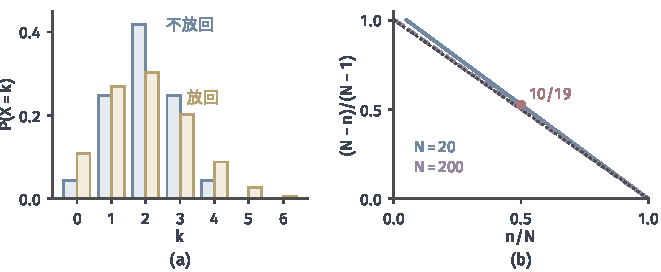
\includegraphics[width=112mm]{figures/07-probability/01-elementary-probability/matplotlib/cdist-hypergeom-binomial/figure.pdf}
  \caption{不放回与放回抽样。(a)$N=20$、$K=4$、$n=10$时次品数的分布：蓝色为$\operatorname{Hyp}(20,4,10)$，黄色为放回抽样的$\operatorname{Bin}(10,0.2)$，两者期望都是$2$。(b)有限总体修正$(N-n)/(N-1)$随抽样比例$n/N$的变化，$N=20$（蓝）与$N=200$（紫，虚线），点线为$1-n/N$；红点是例中的$10/19$。}
  \label{fig:cdist-hypergeom-binomial}
\end{BookInlineFigure}

\paragraph{边界情形}
修正因子在两端退化。$n=N$时因子为零，整箱都被取出，$X$恒等于$K$。$n=1$时因子为一，只抽一个，$X\sim\operatorname{Bern}(K/N)$。$K=0$或$K=N$时箱中只有一类零件，$X$也是常数，式~\eqref{eq:cdist-hypergeometric-var}同样给出零。$N=1$时公式的分母为零，此时$n\in\{0,1\}$，$X$只能是常数或一个Bernoulli变量，直接计算即可。

\paragraph{何时可以用二项分布近似}
总体很大而抽样比例很小时，取走几个零件几乎不改变剩下的构成，不放回与放回就相差无几。设$K/N\to r$且$N\to\infty$，$n$和$k$固定。把式~\eqref{eq:cdist-hypergeometric-pmf}的组合数展开成乘积并重新分组：
\[
  \mathbb{P}(X=k)=\binom{n}{k}
  \prod_{j=0}^{k-1}\frac{K-j}{N-j}\prod_{j=0}^{n-k-1}\frac{N-K-j}{N-k-j}.
\]
第一个乘积的每个因子趋于$r$，第二个乘积的每个因子趋于$1-r$，所以概率趋于$\binom{n}{k}r^{k}(1-r)^{n-k}$。

修正因子告诉我们误差的量级：它约等于$1-n/N$。例如$N=2000$、$K=400$、$n=10$时因子为$1990/1999\approx0.9955$，两个模型的方差只差约$0.5\%$；图~\ref{fig:cdist-hypergeom-binomial}(b)中$N=200$的曲线也几乎贴着$1-n/N$。反过来，抽样比例达到一半时，忽略修正会把方差高估将近一倍。

\subsection{几何分布}
\label{sec:cdist-geometric}

现在换一种记录方式：一个一个检查零件，直到遇到第一个次品为止，记$T$为检查的个数（包括这个次品）。二项分布固定次数、数成功；这里只等一次成功，次数本身成了随机的。

设各次试验相互独立，成功概率都是$p$，并要求$0<p\leq1$。$T=k$意味着前$k-1$次都失败、第$k$次成功，由独立性，这个事件的概率是$(1-p)^{k-1}p$。$p=0$时永远等不到成功，$T$没有定义，所以排除在外；$p=1$时$T$恒为$1$。

\begin{definition}[几何分布]
\label{def:cdist-geometric}
设$0<p\leq1$。若随机变量$T$的质量函数为
\begin{equation}
  \mathbb{P}(T=k)=(1-p)^{k-1}p,\qquad k=1,2,\dots,
  \label{eq:cdist-geometric-pmf}
\end{equation}
则称$T$服从参数为$p$的\term{几何分布}（geometric distribution），记作$T\sim\operatorname{Geom}(p)$。
\end{definition}

这是第一个取值无穷多的模型，总和为一要靠级数。记$q=1-p$，由几何级数$\sum_{k\geq1}q^{k-1}=1/(1-q)$，质量函数之和为$p/(1-q)=1$。

“首次成功晚于第$k$次”等价于“前$k$次全部失败”，所以尾概率有简单的形式：
\begin{equation}
  \mathbb{P}(T>k)=(1-p)^{k},\qquad k=0,1,2,\dots .
  \label{eq:cdist-geometric-tail}
\end{equation}
生产线的例子中$p=0.2$，查了$5$个还没遇到次品的概率是$0.8^{5}\approx0.328$，查了$10$个仍没有的概率约为$0.107$。

\paragraph{期望}
对取正整数值的变量，期望可以写成尾概率之和。把$k$写成$k$个$1$相加，再交换求和次序：
\[
  \mathbb{E}[T]=\sum_{k\geq1}k\,\mathbb{P}(T=k)=\sum_{k\geq1}\sum_{j=1}^{k}\mathbb{P}(T=k)
  =\sum_{j\geq1}\sum_{k\geq j}\mathbb{P}(T=k).
\]
所有项都非负，非负项的二重级数按任何次序求和结果相同，所以交换是允许的。内层和就是$\mathbb{P}(T\geq j)=q^{j-1}$，于是
\[
  \mathbb{E}[T]=\sum_{j\geq1}q^{j-1}=\frac{1}{1-q}=\frac1p .
\]

\paragraph{方差}
二阶矩用同样的办法。把$k^{2}$写成前$k$个奇数之和，$k^{2}=\sum_{j=1}^{k}(2j-1)$，交换次序后
\[
  \mathbb{E}[T^{2}]=\sum_{j\geq1}(2j-1)\,\mathbb{P}(T\geq j)=2\sum_{j\geq1}jq^{j-1}-\sum_{j\geq1}q^{j-1}.
\]
第一个和可以借助刚才的结果，把它看成$\mathbb{E}[T]$除以$p$：
\[
  \sum_{j\geq1}jq^{j-1}=\frac1p\sum_{j\geq1}j\,pq^{j-1}=\frac{\mathbb{E}[T]}{p}=\frac{1}{p^{2}}.
\]
于是
\[
  \mathbb{E}[T^{2}]=\frac{2}{p^{2}}-\frac1p .
\]
减去$(\mathbb{E}[T])^{2}=1/p^{2}$，得到
\begin{equation}
  \mathbb{E}[T]=\frac1p,\qquad \operatorname{Var}(T)=\frac{1-p}{p^{2}} .
  \label{eq:cdist-geometric-moments}
\end{equation}
例中平均要查$5$个，方差为$20$，标准差约$4.47$，与均值相当。等待次数的波动很大：前面算过，查到均值的两倍即$10$个仍未遇到次品，概率还超过十分之一。

\paragraph{无记忆性}
已经连续查了$m$个合格品，还要再查多少个？用条件概率计算。因为$\{T>m+k\}\subseteq\{T>m\}$，交事件就是$\{T>m+k\}$，由式~\eqref{eq:cdist-geometric-tail}，
\[
  \mathbb{P}(T>m+k\mid T>m)=\frac{\mathbb{P}(T>m+k)}{\mathbb{P}(T>m)}=\frac{q^{m+k}}{q^{m}}=q^{k}.
\]
它恰好等于$\mathbb{P}(T>k)$。已经失败了多少次，不影响还要等待的次数的分布，这一性质称为\term{无记忆性}（memorylessness）。

图~\ref{fig:cdist-geometric-memoryless}(b)中，从第$5$次之后重新开始数的条件尾概率（绿点）与原来的尾概率（蓝线）完全重合。“已经连着五个合格，下一个该是次品了”的想法，在独立试验中不成立。反过来，若次品成批出现，前面的结果就携带了信息，无记忆性随独立性一起失去。

\begin{BookInlineFigure}
  \centering
  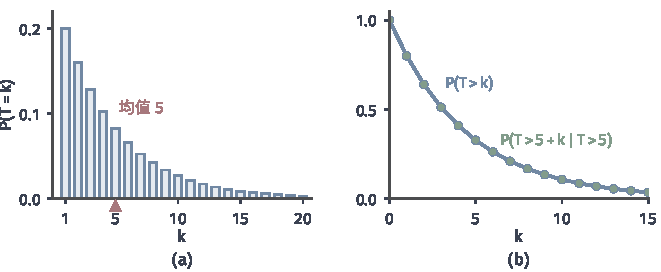
\includegraphics[width=112mm]{figures/07-probability/01-elementary-probability/matplotlib/cdist-geometric-memoryless/figure.pdf}
  \caption{$\operatorname{Geom}(0.2)$。(a)质量函数，红色三角为期望$5$。(b)尾概率$\mathbb{P}(T>k)=0.8^{k}$（蓝）与已知$T>5$后剩余等待的条件尾概率$\mathbb{P}(T>5+k\mid T>5)$（绿点），两者处处相等。}
  \label{fig:cdist-geometric-memoryless}
\end{BookInlineFigure}

无记忆性不只是几何分布的一个性质，它把几何分布完全刻画了出来。

\begin{theorem}[几何分布的无记忆刻画]
\label{thm:cdist-geometric-memoryless}
设$T$取正整数值，且对每个$k\geq0$有$\mathbb{P}(T>k)>0$。若对所有整数$m,k\geq0$都有
\begin{equation}
  \mathbb{P}(T>m+k\mid T>m)=\mathbb{P}(T>k),
  \label{eq:cdist-memoryless-discrete}
\end{equation}
则存在$0<p<1$使$T\sim\operatorname{Geom}(p)$。
\end{theorem}

\begin{proof}
记$G(k)=\mathbb{P}(T>k)$。$T$取正整数值，所以$G(0)=1$。式~\eqref{eq:cdist-memoryless-discrete}左边等于$G(m+k)/G(m)$，于是对所有$m,k\geq0$，
\[
  G(m+k)=G(m)G(k).
\]
取$m=k-1$并对$k$归纳，得到$G(k)=G(1)^{k}$。

记$q=G(1)$，按假设$q>0$。若$q=1$，则$G(k)=1$对所有$k$成立，即$T$大于每一个整数，这与$T$取正整数值矛盾。所以$0<q<1$。令$p=1-q$，则
\[
  \mathbb{P}(T=k)=G(k-1)-G(k)=q^{k-1}-q^{k}=q^{k-1}p,
\]
这正是式~\eqref{eq:cdist-geometric-pmf}。
\end{proof}

\paragraph{另一种计数约定}
也有人记录首次成功之前的失败次数$N=T-1$。它取值于$\{0,1,2,\dots\}$，质量函数为$(1-p)^{k}p$。平移不改变方差，所以
\[
  \mathbb{E}[N]=\frac{1-p}{p},\qquad \operatorname{Var}(N)=\frac{1-p}{p^{2}},
\]
期望比$\mathbb{E}[T]$少$1$。查阅公式时要先确认采用的是哪一种约定，本卷的$\operatorname{Geom}(p)$一律指包含成功那一次的$T$。

\subsection{Poisson分布}
\label{sec:cdist-poisson}

一块钢板表面的划痕数、一小时内到达的故障报警数，都是在固定的范围内计数。这类计数没有事先给定的试验次数，原则上可以取任何非负整数。它们的共同点是：可能发生的机会很多，每个机会发生的概率很小，而且彼此互不影响。

\paragraph{从二项分布出发}
把钢板等分成$n$个小格，假设每格至多有一道划痕，有划痕的概率为$\lambda/n$，各格互不影响。划痕总数服从$\operatorname{Bin}(n,\lambda/n)$，期望固定为$\lambda$。格子分得越细，越接近“任意位置都可能出现划痕”的情形，于是要看$n\to\infty$时质量函数的极限。

\begin{theorem}[二项分布的Poisson极限]
\label{thm:cdist-binomial-poisson}
设$\lambda>0$，$n>\lambda$，$p_n=\lambda/n$。对每个固定的非负整数$k$，
\begin{equation}
  \lim_{n\to\infty}\binom{n}{k}p_n^{k}(1-p_n)^{n-k}=\mathrm{e}^{-\lambda}\frac{\lambda^{k}}{k!}.
  \label{eq:cdist-binomial-poisson}
\end{equation}
\end{theorem}

\begin{proof}
把二项概率拆成四个因子：
\[
  \binom{n}{k}\Bigl(\frac{\lambda}{n}\Bigr)^{k}\Bigl(1-\frac{\lambda}{n}\Bigr)^{n-k}
  =\frac{\lambda^{k}}{k!}\cdot\frac{n(n-1)\cdots(n-k+1)}{n^{k}}
  \cdot\Bigl(1-\frac{\lambda}{n}\Bigr)^{n}\cdot\Bigl(1-\frac{\lambda}{n}\Bigr)^{-k}.
\]
第一个因子与$n$无关。

第二个因子是$k$个分数$(n-j)/n$（$j=0,\dots,k-1$）之积。$k$固定，每个分数趋于$1$，所以乘积趋于$1$。第四个因子同理趋于$1$。

剩下第三个因子。取对数，并令$h=1/n$，
\[
  n\ln\Bigl(1-\frac{\lambda}{n}\Bigr)=\frac{\ln(1-\lambda h)}{h}.
\]
$h\to0$时这是函数$x\mapsto\ln(1-\lambda x)$在$0$处的差商，极限为它的导数$-\lambda$。由指数函数的连续性，第三个因子趋于$\mathrm{e}^{-\lambda}$。四个因子的极限相乘，即得式~\eqref{eq:cdist-binomial-poisson}。
\end{proof}

极限右边对所有$k\geq0$都是正数。它们之和为一，因为由指数函数的幂级数展开，$\sum_{k\geq0}\lambda^{k}/k!=\mathrm{e}^{\lambda}$，这可参考\BookChapterRef{chap:univariate-differentiation}{卷一第6章“一元函数的微分”}。所以极限本身是一个质量函数。

\begin{definition}[Poisson分布]
\label{def:cdist-poisson}
设$\lambda>0$。若随机变量$N$取非负整数值，且
\begin{equation}
  \mathbb{P}(N=k)=\mathrm{e}^{-\lambda}\frac{\lambda^{k}}{k!},\qquad k=0,1,2,\dots,
  \label{eq:cdist-poisson-pmf}
\end{equation}
则称$N$服从参数为$\lambda$的\term{Poisson分布}（Poisson distribution），记作$N\sim\operatorname{Poisson}(\lambda)$。
\end{definition}

\paragraph{期望与方差}
期望的级数中$k=0$一项为零，其余各项约去一个$k$：
\[
  \mathbb{E}[N]=\sum_{k\geq1}k\,\mathrm{e}^{-\lambda}\frac{\lambda^{k}}{k!}
  =\lambda\,\mathrm{e}^{-\lambda}\sum_{k\geq1}\frac{\lambda^{k-1}}{(k-1)!}=\lambda .
\]
二阶矩先算$\mathbb{E}[N(N-1)]$，这样可以约去$k(k-1)$：
\[
  \mathbb{E}[N(N-1)]=\lambda^{2}\mathrm{e}^{-\lambda}\sum_{k\geq2}\frac{\lambda^{k-2}}{(k-2)!}=\lambda^{2}.
\]
于是$\mathbb{E}[N^{2}]=\lambda^{2}+\lambda$，减去$\lambda^{2}$，得到
\begin{equation}
  \mathbb{E}[N]=\operatorname{Var}(N)=\lambda .
  \label{eq:cdist-poisson-moments}
\end{equation}
参数$\lambda$同时是均值和方差。这与二项分布一致：$\operatorname{Bin}(n,\lambda/n)$的方差是$\lambda(1-\lambda/n)$，$n\to\infty$时趋于$\lambda$。

\paragraph{形状}
相邻两项之比为$\mathbb{P}(N=k+1)/\mathbb{P}(N=k)=\lambda/(k+1)$，在$k+1<\lambda$时大于$1$。所以概率一直上升到$\lfloor\lambda\rfloor$附近再下降；$\lambda$为整数时，$\lambda-1$和$\lambda$两处并列最大。$\lambda<1$时最大值在$0$处，质量函数单调下降。图~\ref{fig:cdist-poisson-limit}(a)画出了$\lambda=0.5,2,6$三种形状。

\paragraph{近似的精度}
仍以$\lambda=2$为例，$\operatorname{Poisson}(2)$在$k=0,1,2,3$处的概率为
\[
  0.1353,\quad 0.2707,\quad 0.2707,\quad 0.1804 .
\]
次品数不少于$4$的概率为$1-\frac{19}{3}\mathrm{e}^{-2}\approx0.1429$。

与开头的$\operatorname{Bin}(10,0.2)$相比，零概率$0.1074$与$0.1353$相差较多，因为$10$次试验算不上“机会很多”。改成$\operatorname{Bin}(100,0.02)$，零概率为$0.1326$；改成$\operatorname{Bin}(1000,0.002)$，为$0.1351$。前九项的最大差别依次约为$0.031$、$0.0027$、$0.00027$，大致与$1/n$成比例，见图~\ref{fig:cdist-poisson-limit}(b)。

\begin{BookInlineFigure}
  \centering
  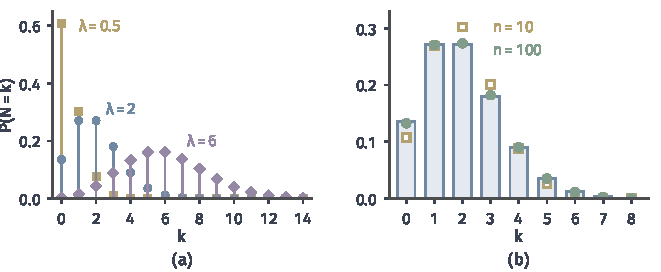
\includegraphics[width=112mm]{figures/07-probability/01-elementary-probability/matplotlib/cdist-poisson-limit/figure.pdf}
  \caption{Poisson分布。(a)$\lambda=0.5$（黄）、$2$（蓝）、$6$（紫）的质量函数。(b)浅蓝柱为$\operatorname{Poisson}(2)$，黄色空心方块为$\operatorname{Bin}(10,0.2)$，绿点为$\operatorname{Bin}(100,0.02)$，后者与柱顶几乎重合。}
  \label{fig:cdist-poisson-limit}
\end{BookInlineFigure}

\paragraph{适用范围}
定理~\ref{thm:cdist-binomial-poisson}说明了Poisson模型的一种来源：机会很多、每次很稀少、彼此独立。仅知道计数非负，并不足以采用Poisson分布。若划痕成簇出现，一道划痕附近往往还有别的，计数的方差会明显大于均值；若计数有明确的上限（例如$10$个零件中的次品数），二项分布更合适。

$\lambda=0$可以作为退化的延伸：按$0^{0}=1$的约定，式~\eqref{eq:cdist-poisson-pmf}给出$\mathbb{P}(N=0)=1$，计数恒为零。这里只把一个固定范围内的计数当作单个随机变量处理；不同时段的计数怎样联合变化、事件何时发生，属于随机过程的问题，不在本章讨论。


\section{连续分布}
\label{sec:cdist-continuous}

连续模型用密度描述概率：区间上的概率是密度在区间上的积分，任何单点的概率都是零。建立一个连续模型，先确定取值范围，即密度为正的区域，称为支撑；再检查密度非负、在整条实轴上的积分等于一；然后用积分计算期望与方差。积分可能发散，所以每个数值特征都要先核对绝对可积，不能凭对称性或公式的样子直接写出。

连续模型的参数往往分工明确。下面的引理说明，把一个随机变量平移和伸缩，密度怎样跟着变化。一般映射下的密度换算在第~\ref{chap:random-variable-transformations}章统一处理，这里只需要最简单的线性情形。

\begin{lemma}[平移与伸缩]
\label{lem:cdist-location-scale}
设$X$有密度$f_X$，$a\in\mathbb{R}$，$s>0$，令$Y=a+sX$。则$Y$有密度
\begin{equation}
  f_Y(y)=\frac1s\,f_X\Bigl(\frac{y-a}{s}\Bigr).
  \label{eq:cdist-location-scale}
\end{equation}
若$X$的期望存在，则$\mathbb{E}[Y]=a+s\,\mathbb{E}[X]$；若$X$的方差有限，则$\operatorname{Var}(Y)=s^{2}\operatorname{Var}(X)$。
\end{lemma}

\begin{proof}
$s>0$，所以$Y\leq y$与$X\leq(y-a)/s$是同一事件。用$X$的密度写出这个概率，再作代换$u=(v-a)/s$，$\mathrm{d}u=\mathrm{d}v/s$：
\[
  \mathbb{P}(Y\leq y)=\int_{-\infty}^{(y-a)/s}f_X(u)\,\mathrm{d}u
  =\int_{-\infty}^{y}\frac1s\,f_X\Bigl(\frac{v-a}{s}\Bigr)\mathrm{d}v .
\]
这对每个$y$成立，所以式~\eqref{eq:cdist-location-scale}是$Y$的密度。期望与方差的变化规律是第~\ref{chap:random-variable-moments}章的平移与缩放法则。
\end{proof}

许多分布族的成员彼此只差一次平移和伸缩。决定平移量的参数称为\term{位置参数}（location parameter），决定伸缩倍数的参数称为\term{尺度参数}（scale parameter），两者都不改变密度曲线的基本形状。改变形状本身的参数称为\term{形状参数}（shape parameter）。

尺度参数与标准差成正比，但比例系数因分布而异，下面会看到，只有高斯分布的惯用参数恰好等于标准差。因此不能把尺度参数一律当作标准差使用。

\subsection{均匀分布}
\label{sec:cdist-uniform}

公交车每$10$分钟一班，乘客在不知道时刻表的情况下随机到站，等待时间$W$落在$0$到$10$分钟之间。如果没有理由认为哪个时刻到站更多，就应当要求等长的时间段有相等的概率。这个要求把密度确定为区间上的常数。

\begin{definition}[均匀分布]
\label{def:cdist-uniform}
设$a<b$。若随机变量$X$的密度为
\begin{equation}
  f_X(x)=
  \begin{cases}
    \dfrac{1}{b-a}, & a<x<b,\\
    0, & \text{其他},
  \end{cases}
  \label{eq:cdist-uniform-density}
\end{equation}
则称$X$服从区间$(a,b)$上的\term{均匀分布}（uniform distribution），记作$X\sim\operatorname{Unif}(a,b)$。
\end{definition}

密度非负，积分是$(b-a)\cdot\frac{1}{b-a}=1$。对$a\leq c<d\leq b$，概率与区间长度成正比：
\[
  \mathbb{P}(c<X<d)=\frac{d-c}{b-a}.
\]
区间外的概率为零。单点的概率也为零：$\mathbb{P}(X=c)$不超过任何包含$c$的小区间的概率$2\varepsilon/(b-a)$，令$\varepsilon\to0$即得。所以区间写成开的还是闭的，不影响任何概率。

分布函数在$(a,b)$上线性上升，两侧分别为$0$和$1$：
\[
  F_X(x)=
  \begin{cases}
    0, & x\leq a,\\
    (x-a)/(b-a), & a<x<b,\\
    1, & x\geq b.
  \end{cases}
\]

等车的例子中$W\sim\operatorname{Unif}(0,10)$，等待超过$7$分钟的概率是$3/10$，即$1-F_W(7)$，图~\ref{fig:cdist-uniform}的两幅子图分别从密度和分布函数读出这个数。

\begin{BookInlineFigure}
  \centering
  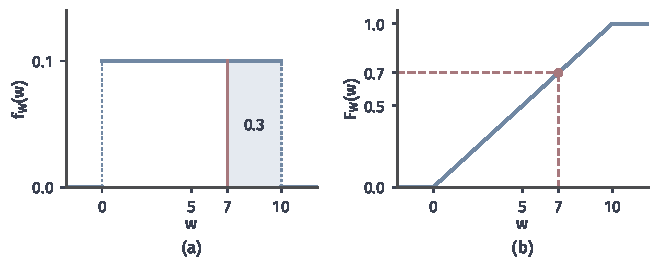
\includegraphics[width=112mm]{figures/07-probability/01-elementary-probability/matplotlib/cdist-uniform/figure.pdf}
  \caption{等待时间$W\sim\operatorname{Unif}(0,10)$。(a)密度，浅蓝面积为$\mathbb{P}(W>7)=0.3$，红线为阈值$7$。(b)分布函数，红点$F_W(7)=0.7$。}
  \label{fig:cdist-uniform}
\end{BookInlineFigure}

\paragraph{期望与方差}
密度关于区间中点对称，期望是中点。直接积分可以验证：
\[
  \mathbb{E}[X]=\frac{1}{b-a}\int_a^bx\,\mathrm{d}x=\frac{b^{2}-a^{2}}{2(b-a)}=\frac{a+b}{2}.
\]
二阶矩为
\[
  \mathbb{E}[X^{2}]=\frac{1}{b-a}\int_a^bx^{2}\,\mathrm{d}x=\frac{b^{3}-a^{3}}{3(b-a)}=\frac{a^{2}+ab+b^{2}}{3}.
\]
减去期望的平方，并把分子通分：
\[
  \operatorname{Var}(X)=\frac{4(a^{2}+ab+b^{2})-3(a+b)^{2}}{12}=\frac{a^{2}-2ab+b^{2}}{12}.
\]
所以
\begin{equation}
  \mathbb{E}[X]=\frac{a+b}{2},\qquad \operatorname{Var}(X)=\frac{(b-a)^{2}}{12}.
  \label{eq:cdist-uniform-moments}
\end{equation}

\paragraph{平移与伸缩}
同一结果可以从$(0,1)$上的均匀分布得到。设$U\sim\operatorname{Unif}(0,1)$，由引理~\ref{lem:cdist-location-scale}，$a+(b-a)U$的密度在$(a,b)$上等于$1/(b-a)$，即$\operatorname{Unif}(a,b)$。$U$的期望为$1/2$、方差为$1/12$，平移不改变方差，伸缩$b-a$倍使方差乘以$(b-a)^{2}$，正好回到式~\eqref{eq:cdist-uniform-moments}。

这里$a$是位置参数，区间长度$b-a$是尺度参数。标准差是$(b-a)/\sqrt{12}\approx0.289(b-a)$，只有区间长度的三成左右。等车的例子中平均等$5$分钟，标准差约$2.89$分钟。

\paragraph{“均匀”需要理由}
均匀分布是一个模型假设，要有“没有位置更特殊”的理由才能采用。乘客若会查看时刻表，到站时刻就集中在发车之前，等待时间不再均匀。均匀分布也只能放在有限区间上：若整条实轴上的密度恒为常数$c$，则$c=0$时积分为零，$c>0$时积分发散，都不能等于一。

\subsection{指数分布}
\label{sec:cdist-exponential}

一台机器在两次故障之间的运行时间$T$是一个连续的等待时间。几何分布描述的是按次计数的等待，这里时间可以取任意正实数。我们希望保留几何分布的无记忆性：已经运行了$s$小时没出故障，剩余时间的分布与新机器相同。下面先给出模型，再说明无记忆性确实把它确定下来。

\begin{definition}[指数分布]
\label{def:cdist-exponential}
设$\lambda>0$。若随机变量$T$的密度为
\begin{equation}
  f_T(t)=\lambda\,\mathrm{e}^{-\lambda t},\quad t\geq0;\qquad f_T(t)=0,\quad t<0,
  \label{eq:cdist-exponential-density}
\end{equation}
则称$T$服从率为$\lambda$的\term{指数分布}（exponential distribution），记作$T\sim\operatorname{Exp}(\lambda)$。参数$\lambda$称为\term{率参数}（rate parameter）。
\end{definition}

密度在$[0,\infty)$上的积分是反常积分，
\[
  \int_0^{\infty}\lambda\,\mathrm{e}^{-\lambda t}\,\mathrm{d}t=\lim_{R\to\infty}\bigl(1-\mathrm{e}^{-\lambda R}\bigr)=1 .
\]
同样的计算给出生存概率，即超过时刻$t$仍在等待的概率：
\begin{equation}
  \mathbb{P}(T>t)=\mathrm{e}^{-\lambda t},\qquad t\geq0 .
  \label{eq:cdist-exponential-survival}
\end{equation}

\paragraph{期望与方差}
各阶矩可以用分部积分逐阶降次。对正整数$k$，在$[0,R]$上分部积分，
\[
  \int_0^{R}t^{k}\lambda\,\mathrm{e}^{-\lambda t}\,\mathrm{d}t
  =-R^{k}\mathrm{e}^{-\lambda R}+\frac{k}{\lambda}\int_0^{R}t^{k-1}\lambda\,\mathrm{e}^{-\lambda t}\,\mathrm{d}t .
\]
$R\to\infty$时边界项趋于零，因为指数衰减快于任何多项式增长；反常积分与分部积分的这些规则可参考\BookChapterRef{chap:univariate-integration}{卷一第7章“一元函数的积分”}。于是
\[
  \mathbb{E}[T^{k}]=\frac{k}{\lambda}\,\mathbb{E}[T^{k-1}],
\]
从$\mathbb{E}[T^{0}]=1$递推得
\begin{equation}
  \mathbb{E}[T^{k}]=\frac{k!}{\lambda^{k}},\qquad k=0,1,2,\dots .
  \label{eq:cdist-exponential-moments-k}
\end{equation}

取$k=1,2$，再用方差的展开式，得到
\begin{equation}
  \mathbb{E}[T]=\frac1\lambda,\qquad \operatorname{Var}(T)=\frac{2}{\lambda^{2}}-\frac{1}{\lambda^{2}}=\frac{1}{\lambda^{2}}.
  \label{eq:cdist-exponential-moments}
\end{equation}
率$\lambda$是单位时间内的平均事件数，均值$1/\lambda$是平均等待时间。$1/\lambda$是尺度参数：$\lambda T\sim\operatorname{Exp}(1)$。指数分布的标准差恰好等于均值。

设机器的故障率为每小时$0.5$次，即$T\sim\operatorname{Exp}(0.5)$。平均运行$2$小时，标准差也是$2$小时，运行超过$3$小时的概率是$\mathrm{e}^{-1.5}\approx0.223$。中位数$m$满足$\mathrm{e}^{-0.5m}=1/2$，即$m=2\ln2\approx1.39$小时，比均值小：少数很长的运行时间把均值拉向右侧。

\paragraph{无记忆性}
已经运行了$s$小时，再运行$t$小时以上的条件概率为
\[
  \mathbb{P}(T>s+t\mid T>s)=\frac{\mathrm{e}^{-\lambda(s+t)}}{\mathrm{e}^{-\lambda s}}=\mathrm{e}^{-\lambda t}=\mathbb{P}(T>t).
\]
例如已经运行$1$小时，再运行$3$小时以上的概率仍是$0.223$，与新机器一样。这里同样用到$\{T>s+t\}\subseteq\{T>s\}$。

与离散情形一样，无记忆性在有密度的非负变量中只属于指数分布。

\begin{theorem}[指数分布的无记忆刻画]
\label{thm:cdist-exponential-memoryless}
设$T$取非负值且有密度，对每个$t\geq0$有$\mathbb{P}(T>t)>0$。若对所有$s,t\geq0$都有
\begin{equation}
  \mathbb{P}(T>s+t\mid T>s)=\mathbb{P}(T>t),
  \label{eq:cdist-memoryless-continuous}
\end{equation}
则存在$\lambda>0$使$T\sim\operatorname{Exp}(\lambda)$。
\end{theorem}

\begin{proof}
记$G(t)=\mathbb{P}(T>t)$。$T$有密度，单点概率为零，所以$G(0)=1$。式~\eqref{eq:cdist-memoryless-continuous}即
\[
  G(s+t)=G(s)G(t),\qquad s,t\geq0 .
\]

先看有理点。对正整数$k,m$，反复使用上式得$G(k/m)=G(1/m)^{k}$，特别地$G(1)=G(1/m)^{m}$。记$c=G(1)>0$，则$G(1/m)=c^{1/m}$，从而
\[
  G(r)=c^{r},\qquad r\text{为正有理数}.
\]

再说明$c<1$。$G(n)=\int_n^{\infty}f_T(u)\,\mathrm{d}u$是收敛反常积分的尾部，$n\to\infty$时趋于零；而$G(n)=c^{n}$，所以$c<1$。

最后看一般的$t>0$。$G$是非增函数，对有理数$r<t<r'$有$c^{r'}\leq G(t)\leq c^{r}$。令$r$与$r'$都趋于$t$，由$r\mapsto c^{r}$的连续性得$G(t)=c^{t}$。令$\lambda=-\ln c>0$，则$G(t)=\mathrm{e}^{-\lambda t}$。生存概率决定分布函数，与式~\eqref{eq:cdist-exponential-survival}比较即知$T\sim\operatorname{Exp}(\lambda)$。
\end{proof}

\paragraph{与几何分布的联系}
指数分布与几何分布可以互相转化。把$T\sim\operatorname{Exp}(\lambda)$向上取整，记$\lceil T\rceil$为运行过的整小时数。对整数$k\geq0$，$\lceil T\rceil>k$与$T>k$是同一事件，所以
\[
  \mathbb{P}(\lceil T\rceil>k)=\mathrm{e}^{-\lambda k}=\bigl(\mathrm{e}^{-\lambda}\bigr)^{k}.
\]
与式~\eqref{eq:cdist-geometric-tail}比较，$\lceil T\rceil\sim\operatorname{Geom}(1-\mathrm{e}^{-\lambda})$。

反过来，把时间切成长为$h$的小段，每段以概率$\lambda h$发生故障，各段独立。等到故障的段数$T_h\sim\operatorname{Geom}(\lambda h)$，等待时间约为$hT_h$。对固定的$t>0$，
\[
  \mathbb{P}(hT_h>t)=(1-\lambda h)^{\lfloor t/h\rfloor}.
\]
取对数，$\lfloor t/h\rfloor$与$t/h$相差不到$1$，而$\ln(1-\lambda h)/h\to-\lambda$，所以上式在$h\to0$时趋于$\mathrm{e}^{-\lambda t}$。指数分布是几何等待在时间连续化之后的极限，见图~\ref{fig:cdist-exponential-geometric}(b)。

\begin{BookInlineFigure}
  \centering
  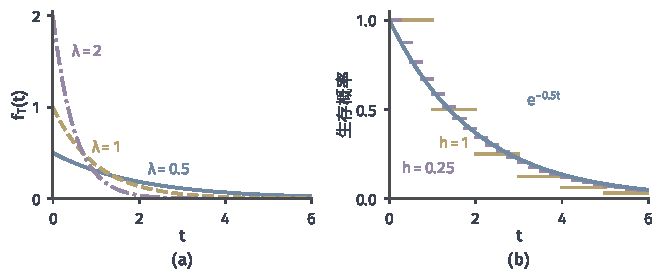
\includegraphics[width=112mm]{figures/07-probability/01-elementary-probability/matplotlib/cdist-exponential-geometric/figure.pdf}
  \caption{指数分布。(a)率$\lambda=0.5$（蓝）、$1$（黄）、$2$（紫）的密度，均值分别为$2,1,0.5$。(b)$\operatorname{Exp}(0.5)$的生存概率$\mathrm{e}^{-0.5t}$（蓝），以及每段长$h$、每段发生概率$0.5h$的几何等待的生存概率：$h=1$（黄）和$h=0.25$（紫）的阶梯随$h$变小贴近蓝线。}
  \label{fig:cdist-exponential-geometric}
\end{BookInlineFigure}

两者的区别也要记清。几何分布取正整数，每个值都有正概率，无记忆性只在整数步上成立；指数分布取连续值，单点概率为零，无记忆性对任意实数$s,t$成立。几何分布的参数$p$是每次试验的概率，不超过$1$；指数分布的$\lambda$是单位时间的率，可以是任意正数，量纲为时间的倒数。

\subsection{高斯分布}
\label{sec:cdist-gaussian}

零件长度的测量值总在标称值附近波动：靠近中心的偏差最常见，偏差越大越少见，正负两侧对称。这样的误差往往是许多微小扰动叠加的结果，它们的和近似服从钟形的分布，第~\ref{chap:central-limit-theorem}章会在明确的条件下证明这一点。这里把钟形密度当作给定的模型，研究它的归一化、参数和区间概率。

钟形由$\mathrm{e}^{-z^{2}/2}$给出。要把它变成密度，先得算出它在整条实轴上的积分。

\begin{lemma}[Gauss积分]
\label{lem:cdist-gauss-integral}
反常积分$\int_{-\infty}^{\infty}\mathrm{e}^{-z^{2}/2}\,\mathrm{d}z$收敛，并且
\begin{equation}
  \int_{-\infty}^{\infty}\mathrm{e}^{-z^{2}/2}\,\mathrm{d}z=\sqrt{2\pi}.
  \label{eq:cdist-gauss-integral}
\end{equation}
\end{lemma}

\begin{proof}
由$(\lvert z\rvert-1)^{2}\geq0$得$z^{2}/2\geq\lvert z\rvert-1/2$，所以被积函数不超过$\mathrm{e}^{1/2}\mathrm{e}^{-\lvert z\rvert}$，积分收敛。记$I_R$为被积函数在$[-R,R]$上的积分，它的平方是正方形$Q_R=[-R,R]^{2}$上的二重积分：
\[
  I_R^{2}=\iint_{Q_R}\mathrm{e}^{-(x^{2}+y^{2})/2}\,\mathrm{d}x\,\mathrm{d}y .
\]

在圆盘上，这个二重积分可以用极坐标算出来。对半径为$\rho$的圆盘$D_\rho$，面积权重为$r$，于是
\[
  \iint_{D_\rho}\mathrm{e}^{-(x^{2}+y^{2})/2}\,\mathrm{d}x\,\mathrm{d}y
  =\int_0^{2\pi}\!\!\int_0^{\rho}\mathrm{e}^{-r^{2}/2}\,r\,\mathrm{d}r\,\mathrm{d}\theta
  =2\pi\bigl(1-\mathrm{e}^{-\rho^{2}/2}\bigr).
\]
极坐标换元可参考\BookChapterRef{chap:region-integrals}{卷二第24章“区域积分”}。

正方形夹在两个圆盘之间：$D_R\subseteq Q_R\subseteq D_{\sqrt2R}$。被积函数为正，区域越大积分越大，所以
\[
  2\pi\bigl(1-\mathrm{e}^{-R^{2}/2}\bigr)\leq I_R^{2}\leq2\pi\bigl(1-\mathrm{e}^{-R^{2}}\bigr).
\]
令$R\to\infty$，两端都趋于$2\pi$，故$I_R^{2}\to2\pi$。$I_R$为正，所以极限是$\sqrt{2\pi}$。
\end{proof}

\begin{definition}[高斯分布]
\label{def:cdist-gaussian}
密度为
\begin{equation}
  \varphi(z)=\frac{1}{\sqrt{2\pi}}\,\mathrm{e}^{-z^{2}/2},\qquad z\in\mathbb{R},
  \label{eq:cdist-standard-gaussian}
\end{equation}
的分布称为\term{标准高斯分布}（standard Gaussian distribution），记作$\mathcal{N}(0,1)$。设$\mu\in\mathbb{R}$，$\sigma>0$。若随机变量$X$的密度为
\begin{equation}
  f_X(x)=\frac{1}{\sqrt{2\pi}\,\sigma}\exp\Bigl(-\frac{(x-\mu)^{2}}{2\sigma^{2}}\Bigr),\qquad x\in\mathbb{R},
  \label{eq:cdist-gaussian-density}
\end{equation}
则称$X$服从\term{高斯分布}（Gaussian distribution），也称正态分布，记作$X\sim\mathcal{N}(\mu,\sigma^{2})$。
\end{definition}

由引理~\ref{lem:cdist-gauss-integral}，$\varphi$的积分为一。比较式~\eqref{eq:cdist-gaussian-density}与式~\eqref{eq:cdist-location-scale}可知，$f_X$正是$\mu+\sigma Z$的密度，其中$Z\sim\mathcal{N}(0,1)$；所以$f_X$的积分也为一。$\mu$是位置参数，$\sigma$是尺度参数：前者平移钟形，后者把它横向拉宽$\sigma$倍、纵向压低$\sigma$倍，见图~\ref{fig:cdist-gaussian}(a)。

\paragraph{期望与方差}
先看标准情形。$\lvert z\rvert\varphi(z)$可积，因为
\[
  \int_0^{\infty}z\,\mathrm{e}^{-z^{2}/2}\,\mathrm{d}z=\Bigl[-\mathrm{e}^{-z^{2}/2}\Bigr]_0^{\infty}=1 .
\]
期望存在，而$z\varphi(z)$是奇函数，两侧相消，所以$\mathbb{E}[Z]=0$。

二阶矩用分部积分。注意$\varphi'(z)=-z\varphi(z)$，把$z^{2}\varphi(z)$写成$z\cdot z\varphi(z)=-z\varphi'(z)$，在$[-R,R]$上分部积分：
\[
  \int_{-R}^{R}z^{2}\varphi(z)\,\mathrm{d}z=\Bigl[-z\varphi(z)\Bigr]_{-R}^{R}+\int_{-R}^{R}\varphi(z)\,\mathrm{d}z .
\]
边界项等于$-2R\varphi(R)$，$R\to\infty$时趋于零，第二项趋于$1$。所以$\mathbb{E}[Z^{2}]=1$，$\operatorname{Var}(Z)=1$。

一般情形由引理~\ref{lem:cdist-location-scale}得到：
\begin{equation}
  \mathbb{E}[X]=\mu,\qquad \operatorname{Var}(X)=\sigma^{2}.
  \label{eq:cdist-gaussian-moments}
\end{equation}
高斯分布的尺度参数$\sigma$恰好是标准差，这是参数化方式带来的巧合，后面的分布都不是这样。

同样的分部积分给出更高阶的矩：$\mathbb{E}[Z^{k+2}]=(k+1)\mathbb{E}[Z^{k}]$，所以$\mathbb{E}[Z^{4}]=3$，奇数阶矩为零。按第~\ref{chap:random-variable-moments}章的定义，高斯分布的偏度为$0$，峰度为$3$，超额峰度约定以它为零点。

\paragraph{区间概率}
标准高斯分布的分布函数记作
\[
  \Phi(z)=\int_{-\infty}^{z}\varphi(u)\,\mathrm{d}u .
\]
它没有初等函数表示，数值要查表或用数值方法算。对称性给出$\Phi(-z)=1-\Phi(z)$，于是只需$z\geq0$的值。几个常用的值是
\[
  \Phi(1)\approx0.8413,\qquad \Phi(1.96)\approx0.9750,\qquad \Phi(2)\approx0.9772 .
\]

一般的$X\sim\mathcal{N}(\mu,\sigma^{2})$先标准化：$X\leq x$等价于$(X-\mu)/\sigma\leq(x-\mu)/\sigma$，而$(X-\mu)/\sigma\sim\mathcal{N}(0,1)$。所以
\begin{equation}
  \mathbb{P}(a<X\leq b)=\Phi\Bigl(\frac{b-\mu}{\sigma}\Bigr)-\Phi\Bigl(\frac{a-\mu}{\sigma}\Bigr).
  \label{eq:cdist-gaussian-interval}
\end{equation}
特别地，落在均值左右$k$个标准差以内的概率是$2\Phi(k)-1$，$k=1,2,3$时依次为
\[
  0.6827,\qquad 0.9545,\qquad 0.9973 .
\]

设零件长度$X\sim\mathcal{N}(10,0.2^{2})$，单位为毫米，合格范围是$[9.8,10.4]$。上下限分别在均值右侧两个标准差和左侧一个标准差处，由式~\eqref{eq:cdist-gaussian-interval}，
\[
  \mathbb{P}(9.8\leq X\leq10.4)=\Phi(2)-\bigl(1-\Phi(1)\bigr)\approx0.9772-0.1587\approx0.819 .
\]
合格范围不对称，所以合格率不能用“$\pm2\sigma$内$95\%$”之类的口诀套算，图~\ref{fig:cdist-gaussian}(b)标出了这块面积。

\begin{BookInlineFigure}
  \centering
  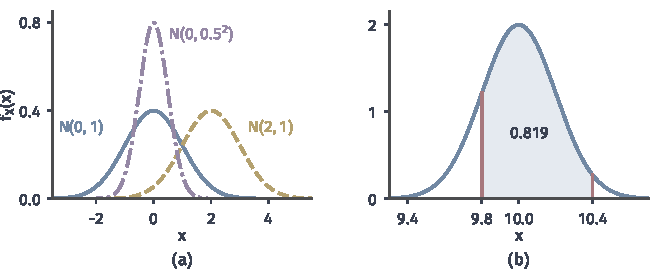
\includegraphics[width=112mm]{figures/07-probability/01-elementary-probability/matplotlib/cdist-gaussian/figure.pdf}
  \caption{高斯分布。(a)$\mathcal{N}(0,1)$（蓝）、平移后的$\mathcal{N}(2,1)$（黄）和尺度减半的$\mathcal{N}(0,0.5^{2})$（紫）。(b)零件长度$\mathcal{N}(10,0.2^{2})$，红线为合格范围的上下限$9.8$与$10.4$（毫米），浅蓝面积为合格率$0.819$。}
  \label{fig:cdist-gaussian}
\end{BookInlineFigure}

\paragraph{尾部}
高斯分布的尾部衰减得极快。对$z>0$，在积分中把$\varphi(u)$放大为$(u/z)\varphi(u)$（因为$u\geq z$），而$u\varphi(u)$有原函数$-\varphi(u)$，得到
\begin{equation}
  1-\Phi(z)\leq\int_z^{\infty}\frac{u}{z}\varphi(u)\,\mathrm{d}u=\frac{\varphi(z)}{z},\qquad z>0 .
  \label{eq:cdist-gaussian-tail}
\end{equation}
尾概率按$\mathrm{e}^{-z^{2}/2}$的速度下降。$z=2$时右端为$0.0270$，真值为$0.0228$；$z=5$时尾概率已不到$3\times10^{-7}$。

这一性质也提醒我们模型的边界。按$\mathcal{N}(10,0.2^{2})$，零件长度为负的概率是$\Phi(-50)$，小到可以忽略，但并不为零；高斯分布在这里是一个近似，并不意味着长度真的可以为负。实际误差若偶尔出现很大的偏离，高斯尾部会严重低估它们的频率，后面的t分布和Laplace分布就是为此准备的。

\subsection{Gamma分布}
\label{sec:cdist-gamma}

指数分布只有一种形状：密度在$0$处最高，然后单调下降。等待第二次、第三次故障的总时间，或者某些只取正值且有偏斜的量，密度往往从零开始先升后降。在指数密度前乘一个幂函数，得到形如$x^{\alpha-1}\mathrm{e}^{-\beta x}$的密度，形状就可以调节。归一化常数需要一个新的函数。

\begin{definition}[Gamma函数]
\label{def:cdist-gamma-function}
对$\alpha>0$，定义
\begin{equation}
  \Gamma(\alpha)=\int_0^{\infty}x^{\alpha-1}\mathrm{e}^{-x}\,\mathrm{d}x .
  \label{eq:cdist-gamma-function}
\end{equation}
称为\term{Gamma函数}（Gamma function）。
\end{definition}

这个反常积分在两端都需要检查。在$0$附近，$x^{\alpha-1}\mathrm{e}^{-x}\leq x^{\alpha-1}$，而$\int_0^1x^{\alpha-1}\,\mathrm{d}x$恰在$\alpha>0$时收敛。在无穷远处，$x^{\alpha-1}\mathrm{e}^{-x/2}$有界，所以被积函数不超过某个常数乘$\mathrm{e}^{-x/2}$，积分收敛。$\alpha\leq0$时$0$附近发散，所以定义要求$\alpha>0$。

\begin{lemma}[Gamma函数的递推]
\label{lem:cdist-gamma-recursion}
对$\alpha>0$，
\begin{equation}
  \Gamma(\alpha+1)=\alpha\,\Gamma(\alpha).
  \label{eq:cdist-gamma-recursion}
\end{equation}
特别地，$\Gamma(1)=1$，对正整数$n$有$\Gamma(n)=(n-1)!$，并且$\Gamma(1/2)=\sqrt\pi$。
\end{lemma}

\begin{proof}
在$[\varepsilon,R]$上分部积分：
\[
  \int_{\varepsilon}^{R}x^{\alpha}\mathrm{e}^{-x}\,\mathrm{d}x
  =\Bigl[-x^{\alpha}\mathrm{e}^{-x}\Bigr]_{\varepsilon}^{R}+\alpha\int_{\varepsilon}^{R}x^{\alpha-1}\mathrm{e}^{-x}\,\mathrm{d}x .
\]
$\varepsilon\to0$、$R\to\infty$时边界项趋于零，即得递推式。$\Gamma(1)$是$\mathrm{e}^{-x}$在$[0,\infty)$上的积分，等于$1$；由递推，$\Gamma(n)=(n-1)\Gamma(n-1)=\dots=(n-1)!$。

对$\Gamma(1/2)$作代换$x=z^{2}/2$，$\mathrm{d}x=z\,\mathrm{d}z$，$x^{-1/2}=\sqrt2/z$：
\[
  \Gamma\Bigl(\frac12\Bigr)=\int_0^{\infty}\frac{\sqrt2}{z}\,\mathrm{e}^{-z^{2}/2}\,z\,\mathrm{d}z=\sqrt2\int_0^{\infty}\mathrm{e}^{-z^{2}/2}\,\mathrm{d}z .
\]
由引理~\ref{lem:cdist-gauss-integral}和对称性，最后的积分是$\sqrt{2\pi}/2$，所以$\Gamma(1/2)=\sqrt\pi$。
\end{proof}

递推式说明Gamma函数把阶乘从正整数延拓到了正实数，图~\ref{fig:cdist-gamma-function}在整数点标出了阶乘。由递推还可以得到半整数处的值，例如$\Gamma(3/2)=\sqrt\pi/2$。

\begin{BookInlineFigure}
  \centering
  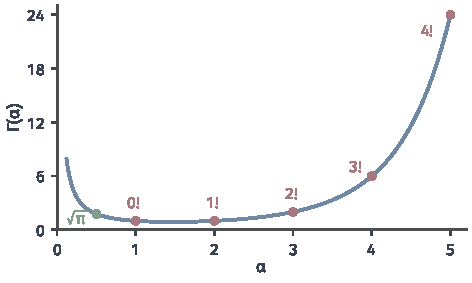
\includegraphics[width=80mm]{figures/07-probability/01-elementary-probability/matplotlib/cdist-gamma-function/figure.pdf}
  \caption{Gamma函数在$(0,5]$上的图像。红点为整数点$\Gamma(n)=(n-1)!$，绿点为$\Gamma(1/2)=\sqrt\pi$。$\alpha\to0^{+}$时$\Gamma(\alpha)\to\infty$。}
  \label{fig:cdist-gamma-function}
\end{BookInlineFigure}

\begin{definition}[Gamma分布]
\label{def:cdist-gamma}
设$\alpha>0$，$\beta>0$。若随机变量$X$的密度为
\begin{equation}
  f_X(x)=\frac{\beta^{\alpha}}{\Gamma(\alpha)}\,x^{\alpha-1}\mathrm{e}^{-\beta x},\quad x>0;\qquad f_X(x)=0,\quad x\leq0,
  \label{eq:cdist-gamma-density}
\end{equation}
则称$X$服从形状为$\alpha$、率为$\beta$的\term{Gamma分布}（Gamma distribution），记作$X\sim\operatorname{Gamma}(\alpha,\beta)$。
\end{definition}

归一化只需一次代换$y=\beta x$：
\[
  \int_0^{\infty}\frac{\beta^{\alpha}}{\Gamma(\alpha)}x^{\alpha-1}\mathrm{e}^{-\beta x}\,\mathrm{d}x
  =\frac{1}{\Gamma(\alpha)}\int_0^{\infty}y^{\alpha-1}\mathrm{e}^{-y}\,\mathrm{d}y=1 .
\]
$\alpha=1$时密度为$\beta\mathrm{e}^{-\beta x}$，就是$\operatorname{Exp}(\beta)$。

\paragraph{期望与方差}
同样的代换给出各阶矩。对$k>-\alpha$，
\[
  \mathbb{E}[X^{k}]=\frac{\beta^{\alpha}}{\Gamma(\alpha)}\int_0^{\infty}x^{\alpha+k-1}\mathrm{e}^{-\beta x}\,\mathrm{d}x
  =\frac{\Gamma(\alpha+k)}{\Gamma(\alpha)\,\beta^{k}} .
\]
取$k=1,2$并用递推式~\eqref{eq:cdist-gamma-recursion}，得到$\mathbb{E}[X]=\alpha/\beta$与$\mathbb{E}[X^{2}]=\alpha(\alpha+1)/\beta^{2}$。于是
\begin{equation}
  \mathbb{E}[X]=\frac{\alpha}{\beta},\qquad \operatorname{Var}(X)=\frac{\alpha(\alpha+1)-\alpha^{2}}{\beta^{2}}=\frac{\alpha}{\beta^{2}}.
  \label{eq:cdist-gamma-moments}
\end{equation}
所有正阶矩都有限。

\paragraph{形状}
形状参数$\alpha$决定密度在$0$附近的行为。$\alpha<1$时$x^{\alpha-1}\to\infty$，密度在$0$处无界，但仍然可积；$\alpha=1$时密度在$0$处取有限正值；$\alpha>1$时密度从$0$出发先升后降。对数导数为$(\alpha-1)/x-\beta$，所以$\alpha>1$时众数为$(\alpha-1)/\beta$。$\alpha$越大，钟形越对称，图~\ref{fig:cdist-gamma-shapes}(a)画出了这几种情形。

$\beta$是率参数，$1/\beta$是尺度参数：由引理~\ref{lem:cdist-location-scale}，$\beta X\sim\operatorname{Gamma}(\alpha,1)$。改变$\beta$只把同一形状横向伸缩。

\begin{BookInlineFigure}
  \centering
  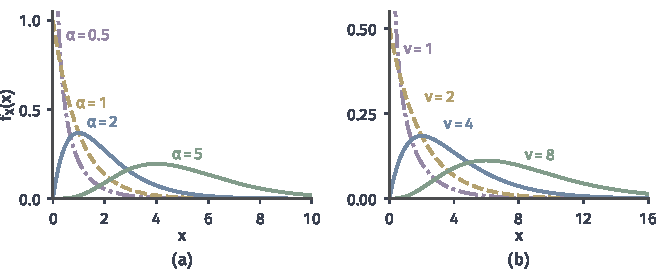
\includegraphics[width=112mm]{figures/07-probability/01-elementary-probability/matplotlib/cdist-gamma-shapes/figure.pdf}
  \caption{Gamma分布的形状。(a)率$\beta=1$，形状$\alpha=0.5$（紫，$0$处无界）、$1$（黄，即$\operatorname{Exp}(1)$）、$2$（蓝）、$5$（绿）。(b)卡方分布$\chi^{2}_{\nu}=\operatorname{Gamma}(\nu/2,1/2)$，$\nu=1,2,4,8$，配色同(a)。}
  \label{fig:cdist-gamma-shapes}
\end{BookInlineFigure}

设故障率为每小时$0.5$次。等待第二次故障的时间$X$常用形状$\alpha=2$、率$\beta=0.5$的Gamma分布描述；它为什么是两段独立指数等待之和的分布，第~\ref{chap:random-variable-transformations}章会给出证明。期望为$4$小时，方差为$8$，众数为$2$小时。超过$4$小时的概率由分部积分算出：
\[
  \mathbb{P}(X>4)=\int_4^{\infty}\frac{x}{4}\,\mathrm{e}^{-x/2}\,\mathrm{d}x
  =\Bigl[-\frac{x}{2}\mathrm{e}^{-x/2}-\mathrm{e}^{-x/2}\Bigr]_4^{\infty}=3\mathrm{e}^{-2}\approx0.406 .
\]

\paragraph{率与尺度两种写法}
不少文献改用尺度$\theta=1/\beta$作参数，密度写成
\[
  f_X(x)=\frac{1}{\Gamma(\alpha)\,\theta^{\alpha}}\,x^{\alpha-1}\mathrm{e}^{-x/\theta},\qquad x>0,
\]
此时期望为$\alpha\theta$，方差为$\alpha\theta^{2}$。同一个记号$\operatorname{Gamma}(2,0.5)$，按率理解期望是$4$，按尺度理解期望是$1$，相差四倍。本卷一律使用率$\beta$。还要注意标准差是$\sqrt\alpha\,\theta$，只有$\alpha=1$时才等于尺度$\theta$。

\paragraph{卡方分布}
Gamma族中有一个特例经常单独出现。对$\nu>0$，形状为$\nu/2$、率为$1/2$的Gamma分布称为自由度为$\nu$的\term{卡方分布}（chi-squared distribution），记作$\chi^{2}_{\nu}$。由式~\eqref{eq:cdist-gamma-moments}，
\begin{equation}
  \mathbb{E}[X]=\nu,\qquad \operatorname{Var}(X)=2\nu,\qquad X\sim\chi^{2}_{\nu}.
  \label{eq:cdist-chisq-moments}
\end{equation}
名称中的“平方”来自它的构造：$\nu$为正整数时，$\nu$个相互独立的标准高斯变量的平方和服从$\chi^{2}_{\nu}$，这一结论在第~\ref{chap:random-variable-transformations}章证明。这里的定义对任意正实数$\nu$都有意义。

\subsection{Beta分布}
\label{sec:cdist-beta}

一批货中次品所占的比例、一次投篮的命中率，都是落在$0$与$1$之间的量。若这些比例本身随批次而变，就需要$(0,1)$上的分布来描述。仿照Gamma分布，在两个端点各放一个幂函数，得到形如$x^{a-1}(1-x)^{b-1}$的密度，两个指数分别控制密度在$0$和$1$附近的行为。为避免与Gamma分布的率$\beta$混淆，这里的参数记作$a,b$。

\begin{definition}[Beta函数与Beta分布]
\label{def:cdist-beta}
对$a>0$，$b>0$，称
\begin{equation}
  \mathrm{B}(a,b)=\int_0^{1}x^{a-1}(1-x)^{b-1}\,\mathrm{d}x
  \label{eq:cdist-beta-function}
\end{equation}
为\term{Beta函数}（Beta function）。若随机变量$X$的密度为
\begin{equation}
  f_X(x)=\frac{x^{a-1}(1-x)^{b-1}}{\mathrm{B}(a,b)},\quad 0<x<1;\qquad f_X(x)=0,\quad\text{其他},
  \label{eq:cdist-beta-density}
\end{equation}
则称$X$服从\term{Beta分布}（Beta distribution），记作$X\sim\operatorname{Beta}(a,b)$。
\end{definition}

积分~\eqref{eq:cdist-beta-function}在$0$附近的被积函数与$x^{a-1}$同阶，在$1$附近与$(1-x)^{b-1}$同阶，所以恰在$a>0$且$b>0$时收敛。密度的归一化由定义直接保证，计算期望和方差则需要Beta函数的两条性质。

\begin{lemma}[Beta函数的性质]
\label{lem:cdist-beta-function}
对$a,b>0$，
\begin{equation}
  \mathrm{B}(a+1,b)=\frac{a}{a+b}\,\mathrm{B}(a,b),
  \label{eq:cdist-beta-recursion}
\end{equation}
并且
\begin{equation}
  \mathrm{B}(a,b)=\frac{\Gamma(a)\,\Gamma(b)}{\Gamma(a+b)} .
  \label{eq:cdist-beta-gamma}
\end{equation}
\end{lemma}

\begin{proof}
先证递推式。被积函数乘以$x+(1-x)=1$再拆开，得到
\[
  \mathrm{B}(a,b)=\mathrm{B}(a+1,b)+\mathrm{B}(a,b+1).
\]
另一方面，对$\mathrm{B}(a+1,b)$分部积分，把$(1-x)^{b-1}$积成$-(1-x)^{b}/b$，边界项在两端为零：
\[
  \begin{aligned}
  \mathrm{B}(a+1,b)&=\int_0^{1}x^{a}(1-x)^{b-1}\,\mathrm{d}x\\
  &=\frac{a}{b}\int_0^{1}x^{a-1}(1-x)^{b}\,\mathrm{d}x=\frac{a}{b}\,\mathrm{B}(a,b+1).
  \end{aligned}
\]
把$\mathrm{B}(a,b+1)=\frac{b}{a}\mathrm{B}(a+1,b)$代入第一式，得到
\[
  \mathrm{B}(a,b)=\Bigl(1+\frac{b}{a}\Bigr)\mathrm{B}(a+1,b)=\frac{a+b}{a}\,\mathrm{B}(a+1,b),
\]
即式~\eqref{eq:cdist-beta-recursion}。

再证式~\eqref{eq:cdist-beta-gamma}。把两个Gamma积分之积写成第一象限上的二重积分：
\[
  \Gamma(a)\Gamma(b)=\int_0^{\infty}\!\!\int_0^{\infty}x^{a-1}y^{b-1}\mathrm{e}^{-(x+y)}\,\mathrm{d}x\,\mathrm{d}y .
\]
被积函数为正，这一步以及下面的换元都可以先在有界区域上进行，再令区域扩大取极限。

作代换$x=st$，$y=s(1-t)$，其中$s>0$，$0<t<1$。它把$(0,\infty)\times(0,1)$一一映到第一象限，逆映射为$s=x+y$，$t=x/(x+y)$。Jacobian行列式为
\[
  \det\begin{pmatrix}t & s\\ 1-t & -s\end{pmatrix}=-ts-s(1-t)=-s,
\]
绝对值为$s$。代入后被积函数分离成$s$的函数与$t$的函数之积：
\[
  \Gamma(a)\Gamma(b)=\int_0^{\infty}s^{a+b-1}\mathrm{e}^{-s}\,\mathrm{d}s\int_0^{1}t^{a-1}(1-t)^{b-1}\,\mathrm{d}t
  =\Gamma(a+b)\,\mathrm{B}(a,b).
\]
\end{proof}

\paragraph{期望与方差}
期望是两个Beta函数之比，由式~\eqref{eq:cdist-beta-recursion}，
\[
  \mathbb{E}[X]=\frac{\mathrm{B}(a+1,b)}{\mathrm{B}(a,b)}=\frac{a}{a+b}.
\]
二阶矩连用两次递推，第二次的参数是$(a+1,b)$：
\[
  \mathbb{E}[X^{2}]=\frac{\mathrm{B}(a+2,b)}{\mathrm{B}(a,b)}=\frac{a+1}{a+b+1}\cdot\frac{a}{a+b}.
\]
减去期望的平方并通分，分子化为$a[(a+1)(a+b)-a(a+b+1)]=ab$，所以
\begin{equation}
  \mathbb{E}[X]=\frac{a}{a+b},\qquad \operatorname{Var}(X)=\frac{ab}{(a+b)^{2}(a+b+1)} .
  \label{eq:cdist-beta-moments}
\end{equation}

\paragraph{端点形状}
参数$a$管左端，$b$管右端。$a<1$时密度在$0$附近无界，$a=1$时在$0$处取有限正值$b$，$a>1$时在$0$处为零；$b$对右端同理。几个特殊情形一目了然：$\operatorname{Beta}(1,1)$就是$\operatorname{Unif}(0,1)$；$a=b$时密度关于$1/2$对称；$a=b<1$时呈U形，比例倾向于靠近两端。$a,b>1$时众数为$(a-1)/(a+b-2)$。这些形状画在图~\ref{fig:cdist-beta-shapes}(a)中。

\paragraph{集中程度}
期望只取决于比值$a/(a+b)$，集中程度则由总和决定。记$m=a/(a+b)$，$\kappa=a+b$，式~\eqref{eq:cdist-beta-moments}中的方差可以改写为
\begin{equation}
  \operatorname{Var}(X)=\frac{m(1-m)}{\kappa+1}.
  \label{eq:cdist-beta-concentration}
\end{equation}
固定$m=0.2$，$\kappa=2.5,10,50$对应的方差依次约为$0.0457$、$0.0145$、$0.0031$：$\kappa$越大，比例越紧地聚在$0.2$附近，见图~\ref{fig:cdist-beta-shapes}(b)。

\begin{BookInlineFigure}
  \centering
  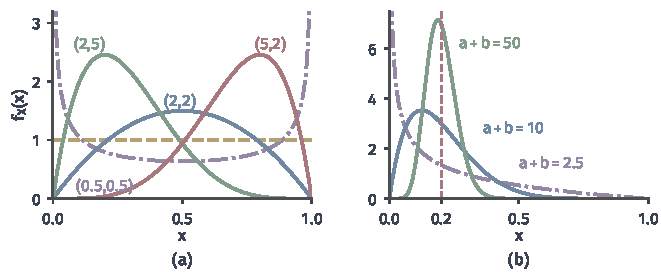
\includegraphics[width=112mm]{figures/07-probability/01-elementary-probability/matplotlib/cdist-beta-shapes/figure.pdf}
  \caption{Beta分布。(a)参数$(a,b)$为$(0.5,0.5)$（紫，U形）、$(1,1)$（黄色虚线，均匀分布）、$(2,2)$（蓝）、$(2,5)$（绿）、$(5,2)$（红）。(b)期望固定为$0.2$（红色虚线），$a+b=2.5,10,50$。}
  \label{fig:cdist-beta-shapes}
\end{BookInlineFigure}

以$X\sim\operatorname{Beta}(2,8)$描述各批次的次品比例，期望为$0.2$，方差约$0.0145$，标准差约$0.12$。由式~\eqref{eq:cdist-beta-gamma}，$\mathrm{B}(2,8)=1!\,7!/9!=1/72$。某批次比例超过$0.4$的概率为
\[
  \mathbb{P}(X>0.4)=72\int_{0.4}^{1}x(1-x)^{7}\,\mathrm{d}x .
\]
令$u=1-x$，积分化为
\[
  \int_0^{0.6}(1-u)u^{7}\,\mathrm{d}u=\frac{0.6^{8}}{8}-\frac{0.6^{9}}{9}\approx0.000980,
\]
乘以$72$得$\mathbb{P}(X>0.4)\approx0.0705$。

Beta分布描述的是一个比例的分布，与二项分布描述的次品个数是两回事：前者连续地取$(0,1)$中的值，后者在给定比例下数个数。多个比例同时变化、总和为一的情形，由第~\ref{chap:multivariate-distributions}章的Dirichlet分布推广；那里还会说明，两个相互独立、率相同的Gamma变量中，一个占两者之和的比例服从Beta分布。

\subsection{Student t分布}
\label{sec:cdist-t}

高斯模型的尾部衰减得太快：偏离$5$个标准差的概率不到$10^{-6}$。如果测量偶尔受到较大的干扰，这样的偏离会比高斯模型预言的多得多。我们想要一个仍然对称、钟形，但尾部只按幂函数衰减的密度。

把$\mathrm{e}^{-z^{2}/2}$换成$(1+z^{2}/\nu)^{-(\nu+1)/2}$就能做到。$z$很大时它与$\lvert z\rvert^{-(\nu+1)}$同阶，衰减比指数慢得多；$\nu$越大，它越像$\mathrm{e}^{-z^{2}/2}$。先算归一化常数。

\begin{lemma}[t密度的归一化]
\label{lem:cdist-t-normalization}
对$\nu>0$，
\begin{equation}
  \int_{-\infty}^{\infty}\Bigl(1+\frac{z^{2}}{\nu}\Bigr)^{-(\nu+1)/2}\mathrm{d}z
  =\sqrt\nu\,\mathrm{B}\Bigl(\frac12,\frac\nu2\Bigr)
  =\frac{\sqrt{\nu\pi}\,\Gamma(\nu/2)}{\Gamma((\nu+1)/2)} .
  \label{eq:cdist-t-normalization}
\end{equation}
\end{lemma}

\begin{proof}
被积函数是偶函数，只算$z>0$的一半再乘以$2$。令$y=z^{2}/\nu$，则$z=\sqrt{\nu y}$，并且
\[
  \mathrm{d}z=\frac{\sqrt\nu}{2\sqrt y}\,\mathrm{d}y .
\]
于是
\[
  2\int_0^{\infty}\Bigl(1+\frac{z^{2}}{\nu}\Bigr)^{-\frac{\nu+1}{2}}\mathrm{d}z
  =\sqrt\nu\int_0^{\infty}y^{-1/2}(1+y)^{-\frac{\nu+1}{2}}\,\mathrm{d}y .
\]

再令$y=t/(1-t)$，$0<t<1$。此时$1+y=1/(1-t)$，$\mathrm{d}y=\mathrm{d}t/(1-t)^{2}$，被积函数中$t$的幂次为$-1/2$，$1-t$的幂次为
\[
  \frac12+\frac{\nu+1}{2}-2=\frac\nu2-1 .
\]
所以右端的积分等于$\mathrm{B}(1/2,\nu/2)$。最后由式~\eqref{eq:cdist-beta-gamma}和$\Gamma(1/2)=\sqrt\pi$得到第二个等号。
\end{proof}

\begin{definition}[Student t分布]
\label{def:cdist-t}
设$\nu>0$，$\mu\in\mathbb{R}$，$s>0$，记
\begin{equation}
  c_\nu=\frac{\Gamma((\nu+1)/2)}{\sqrt{\nu\pi}\,\Gamma(\nu/2)} .
  \label{eq:cdist-t-constant}
\end{equation}
若随机变量$X$的密度为
\begin{equation}
  f_X(x)=\frac{c_\nu}{s}\Bigl(1+\frac{(x-\mu)^{2}}{\nu s^{2}}\Bigr)^{-(\nu+1)/2},\qquad x\in\mathbb{R},
  \label{eq:cdist-t-density}
\end{equation}
则称$X$服从自由度为$\nu$、位置为$\mu$、尺度为$s$的\term{Student t分布}（Student's t distribution），记作$X\sim t_{\nu}(\mu,s^{2})$。$\mu=0$、$s=1$时称为标准t分布，记作$t_{\nu}$。
\end{definition}

由引理~\ref{lem:cdist-t-normalization}，标准t密度的积分为一；一般情形是$\mu+sT$（$T\sim t_\nu$）的密度，由引理~\ref{lem:cdist-location-scale}，积分也为一。参数$\nu$称为\term{自由度}（degrees of freedom），它是形状参数，控制尾部的厚薄。

\paragraph{矩的存在条件}
t分布与前面各模型最大的不同在于矩可能不存在。对标准t变量$T$，当$\lvert z\rvert\geq\sqrt\nu$时，$z^{2}/\nu\leq1+z^{2}/\nu\leq2z^{2}/\nu$，所以密度被夹在$\lvert z\rvert^{-(\nu+1)}$的两个常数倍之间：
\[
  c_\nu\Bigl(\frac{2}{\nu}\Bigr)^{-\frac{\nu+1}{2}}\lvert z\rvert^{-(\nu+1)}
  \leq c_\nu\Bigl(1+\frac{z^{2}}{\nu}\Bigr)^{-\frac{\nu+1}{2}}
  \leq c_\nu\,\nu^{\frac{\nu+1}{2}}\lvert z\rvert^{-(\nu+1)}.
\]

于是对$r>0$，$\mathbb{E}\lvert T\rvert^{r}$的有限与否取决于$\int_{\sqrt\nu}^{\infty}z^{r-\nu-1}\,\mathrm{d}z$，由反常积分的比较判别，它恰在$r<\nu$时收敛。结论是
\begin{equation}
  \mathbb{E}\lvert T\rvert^{r}<\infty\iff r<\nu .
  \label{eq:cdist-t-moment-existence}
\end{equation}
所以$\nu>1$时期望存在，由对称性等于$0$；$\nu>2$时方差有限；$\nu\leq1$时期望不存在。自由度越小，存在的矩越少。

\paragraph{期望与方差}
设$\nu>2$。计算$\mathbb{E}[T^{2}]$用的代换与引理~\ref{lem:cdist-t-normalization}相同，只是被积函数多了因子$z^{2}=\nu y$，$y$的幂次从$-1/2$变成$1/2$。逐步代换后，$t$的幂次为$1/2$，$1-t$的幂次为$\nu/2-2$，于是
\[
  \int_{-\infty}^{\infty}z^{2}\Bigl(1+\frac{z^{2}}{\nu}\Bigr)^{-\frac{\nu+1}{2}}\mathrm{d}z
  =\nu^{3/2}\,\mathrm{B}\Bigl(\frac32,\frac\nu2-1\Bigr),
\]
其中$\nu/2-1>0$正是$\nu>2$的条件。

除以式~\eqref{eq:cdist-t-normalization}的归一化常数，再用式~\eqref{eq:cdist-beta-gamma}把Beta函数化成Gamma函数，分子分母中的$\Gamma((\nu+1)/2)$约去：
\[
  \mathbb{E}[T^{2}]=\nu\,\frac{\Gamma(3/2)\,\Gamma(\nu/2-1)}{\Gamma(1/2)\,\Gamma(\nu/2)}
  =\nu\cdot\frac12\cdot\frac{1}{\nu/2-1}=\frac{\nu}{\nu-2},
\]
这里用了$\Gamma(3/2)=\frac12\Gamma(1/2)$和$\Gamma(\nu/2)=(\nu/2-1)\Gamma(\nu/2-1)$。

由引理~\ref{lem:cdist-location-scale}，对$X\sim t_{\nu}(\mu,s^{2})$，
\begin{equation}
  \mathbb{E}[X]=\mu\quad(\nu>1),\qquad \operatorname{Var}(X)=s^{2}\frac{\nu}{\nu-2}\quad(\nu>2).
  \label{eq:cdist-t-moments}
\end{equation}
$1<\nu\leq2$时期望为$\mu$而方差为无穷大。尺度$s$不是标准差：$\nu=3$时标准差是$\sqrt3\,s$，$\nu=5$时是$\sqrt{5/3}\,s$。

\paragraph{Cauchy分布}
$\nu=1$的情形单独称为\term{Cauchy分布}（Cauchy distribution）。此时$c_1=\Gamma(1)/(\sqrt\pi\,\Gamma(1/2))=1/\pi$，标准情形的密度为
\begin{equation}
  f(x)=\frac{1}{\pi(1+x^{2})},\qquad x\in\mathbb{R}.
  \label{eq:cdist-cauchy-density}
\end{equation}
它关于$0$对称，但期望不存在。正半轴上的积分发散：
\[
  \int_0^{R}\frac{x}{\pi(1+x^{2})}\,\mathrm{d}x=\frac{1}{2\pi}\ln(1+R^{2})\to\infty .
\]
负半轴同样发散，正负两部分都是无穷大，按第~\ref{chap:random-variable-moments}章的规定，期望没有定义。

对称性诱使人说“期望是$0$”，可以用不对称的截断看出这为何不行。把积分区间取成$[-R,cR]$，$c>0$，则
\[
  \int_{-R}^{cR}\frac{x}{\pi(1+x^{2})}\,\mathrm{d}x=\frac{1}{2\pi}\ln\frac{1+c^{2}R^{2}}{1+R^{2}}\to\frac{\ln c}{\pi}\qquad(R\to\infty).
\]
对称截断（$c=1$）给出$0$，$c=2$给出$\ln2/\pi\approx0.221$，$c=1/2$给出$-0.221$。极限依赖于截断的方式，说明这里没有一个确定的“平均位置”，见图~\ref{fig:cdist-cauchy-truncation}。

\begin{BookInlineFigure}
  \centering
  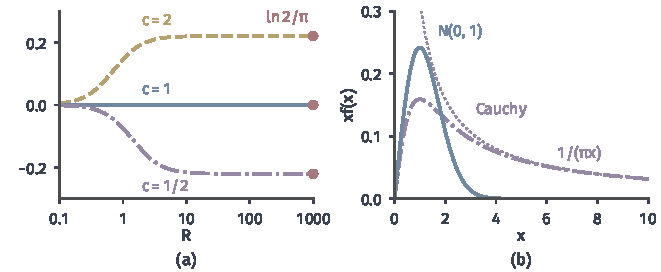
\includegraphics[width=112mm]{figures/07-probability/01-elementary-probability/matplotlib/cdist-cauchy-truncation/figure.pdf}
  \caption{Cauchy分布的期望不存在。(a)截断积分$\int_{-R}^{cR}xf(x)\,\mathrm{d}x$随$R$的变化，$c=2$（黄）、$1$（蓝）、$1/2$（紫），横轴为对数刻度，红点为三个不同的极限$\ln c/\pi$。(b)$xf(x)$：Cauchy分布（紫）按$1/(\pi x)$（紫色点线）衰减，积分发散；$\mathcal{N}(0,1)$（蓝）很快衰减到零。}
  \label{fig:cdist-cauchy-truncation}
\end{BookInlineFigure}

Cauchy分布的位置要用中位数描述。标准情形的分布函数为$F(x)=\frac12+\frac1\pi\arctan x$，中位数是$0$，上下四分位数是$\pm1$。所以$t_1(\mu,s^{2})$的中位数是$\mu$，尺度$s$恰好是四分位距的一半：$\mu$是对称中心与中位数，但不是期望。

\paragraph{与高斯分布的关系}
$\nu\to\infty$时t密度趋于标准高斯密度。函数部分取对数，与定理~\ref{thm:cdist-binomial-poisson}证明中的方法相同：
\[
  -\frac{\nu+1}{2}\ln\Bigl(1+\frac{z^{2}}{\nu}\Bigr)\to-\frac{z^{2}}{2}.
\]
式~\eqref{eq:cdist-t-constant}中的常数$c_\nu$趋于$1/\sqrt{2\pi}\approx0.3989$，证明需要Gamma函数的渐近公式，这里只列出数值：$\nu=1,3,10,30,100$时依次约为$0.3183$、$0.3676$、$0.3891$、$0.3956$、$0.3979$。

图~\ref{fig:cdist-t-tails}(a)中$\nu=30$的t密度已与高斯密度几乎重合，差别集中在尾部。图~\ref{fig:cdist-t-tails}(b)用对数纵轴画出双侧尾概率：$\mathbb{P}(\lvert T\rvert>3)$在高斯、$t_3$和Cauchy情形分别约为$0.0027$、$0.0577$、$0.2048$，差了两个数量级。

\begin{BookInlineFigure}
  \centering
  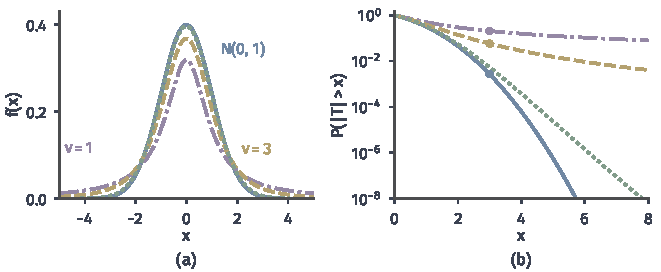
\includegraphics[width=112mm]{figures/07-probability/01-elementary-probability/matplotlib/cdist-t-tails/figure.pdf}
  \caption{t分布与高斯分布。(a)标准高斯（蓝）与$\nu=1$（紫）、$\nu=3$（黄）、$\nu=30$（绿色点线，几乎与蓝线重合）的标准t密度。(b)双侧尾概率$\mathbb{P}(\lvert T\rvert>x)$，纵轴为对数刻度，圆点为$x=3$处的值；高斯尾部按$\mathrm{e}^{-x^{2}/2}$下降，t分布按幂函数下降。}
  \label{fig:cdist-t-tails}
\end{BookInlineFigure}

t分布还可以由高斯变量构造：设$Z\sim\mathcal{N}(0,1)$与$U\sim\chi^{2}_{\nu}$相互独立，则$Z/\sqrt{U/\nu}\sim t_\nu$。这相当于给高斯变量配上一个随机的尺度，尺度偶尔变得很大，就产生了厚尾。这个比值的分布在第~\ref{chap:random-variable-transformations}章推导，多个分量共享同一随机尺度的情形见第~\ref{chap:multivariate-distributions}章。

\subsection{Laplace分布}
\label{sec:cdist-laplace}

另一种加厚尾部的办法是把高斯密度指数中的平方换成绝对值。$\mathrm{e}^{-\lvert x\rvert}$在原点有一个尖角，尾部按指数而不是按$\mathrm{e}^{-x^{2}/2}$衰减：比高斯厚，但仍比任何幂函数薄。

\begin{definition}[Laplace分布]
\label{def:cdist-laplace}
设$\mu\in\mathbb{R}$，$b>0$。若随机变量$X$的密度为
\begin{equation}
  f_X(x)=\frac{1}{2b}\exp\Bigl(-\frac{\lvert x-\mu\rvert}{b}\Bigr),\qquad x\in\mathbb{R},
  \label{eq:cdist-laplace-density}
\end{equation}
则称$X$服从参数为$\mu,b$的\term{Laplace分布}（Laplace distribution），记作$X\sim\operatorname{Laplace}(\mu,b)$。
\end{definition}

$\mu$是位置参数，$b$是尺度参数。标准情形$\mu=0$、$b=1$的密度是$\frac12\mathrm{e}^{-\lvert z\rvert}$，分成正负两半各积一次指数，每半的积分是$1/2$，总和为一。右半边恰好是率为$1$的指数密度的一半，这也是它又叫双指数分布的原因：给定$X>\mu$，$X-\mu$服从$\operatorname{Exp}(1/b)$。

\paragraph{期望与方差}
对标准情形$Z$，绝对矩可以用Gamma函数算出：
\[
  \mathbb{E}\lvert Z\rvert^{k}=2\int_0^{\infty}z^{k}\cdot\frac12\mathrm{e}^{-z}\,\mathrm{d}z=\Gamma(k+1)=k!,\qquad k=0,1,2,\dots .
\]
所有阶的矩都有限。密度对称，所以$\mathbb{E}[Z]=0$，$\operatorname{Var}(Z)=\mathbb{E}[Z^{2}]=2$。由引理~\ref{lem:cdist-location-scale}，
\begin{equation}
  \mathbb{E}[X]=\mu,\qquad \operatorname{Var}(X)=2b^{2}.
  \label{eq:cdist-laplace-moments}
\end{equation}
标准差为$\sqrt2\,b$，尺度$b$同样不是标准差。四阶中心矩为$24b^{4}$，峰度为$24b^{4}/(2b^{2})^{2}=6$，比高斯分布的$3$大$3$。

尾概率也有简单的形式。分两侧积分，
\begin{equation}
  \mathbb{P}(\lvert X-\mu\rvert>t)=\mathrm{e}^{-t/b},\qquad t\geq0 .
  \label{eq:cdist-laplace-tail}
\end{equation}

\paragraph{与高斯分布的比较}
比较形状要在相同的方差下进行，否则只是尺度不同。取方差都为$1$：$\mathcal{N}(0,1)$与$\operatorname{Laplace}(0,1/\sqrt2)$。两者的峰值分别是$1/\sqrt{2\pi}\approx0.399$和$1/\sqrt2\approx0.707$，Laplace分布的中心更尖。

两条密度曲线在$\lvert x\rvert\approx0.49$和$\lvert x\rvert\approx2.34$处相交。中间一段（$0.49<\lvert x\rvert<2.34$）高斯密度更高，两端Laplace密度更高，所以Laplace分布同时有更尖的中心、更薄的“肩部”和更厚的尾部。方差相同，质量的分布方式却不同。

到远处差别更明显。由式~\eqref{eq:cdist-laplace-tail}，偏离超过$3$个标准差的概率为$\mathrm{e}^{-3\sqrt2}\approx0.0144$，是高斯分布$0.0027$的五倍多；超过$5$个标准差时，Laplace约为$8.5\times10^{-4}$，高斯不到$6\times10^{-7}$。在对数纵轴上，Laplace的对数密度在$x>0$一侧是直线，高斯的是向下弯的抛物线，见图~\ref{fig:cdist-laplace-normal}(b)。

\begin{BookInlineFigure}
  \centering
  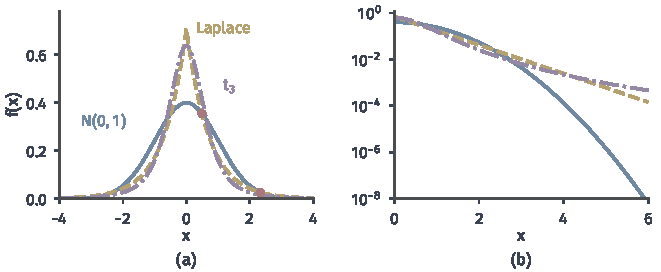
\includegraphics[width=112mm]{figures/07-probability/01-elementary-probability/matplotlib/cdist-laplace-normal/figure.pdf}
  \caption{方差都为$1$的三种对称分布：$\mathcal{N}(0,1)$（蓝）、$\operatorname{Laplace}(0,1/\sqrt2)$（黄）和尺度为$1/\sqrt3$的$t_3$（紫）。(a)密度，红点为高斯与Laplace密度在右侧的两个交点。(b)$x\geq0$部分的对数密度。}
  \label{fig:cdist-laplace-normal}
\end{BookInlineFigure}

图中还画了方差同为$1$的$t_3$分布。它的中心与Laplace相近，在$3$个标准差处的双侧尾概率约为$0.0138$，也与Laplace相当；到$5$个标准差处约为$0.0032$，已是Laplace的近四倍，因为幂函数尾部最终总比指数尾部厚。Laplace分布有全部阶的矩，$t_3$的四阶矩却是无穷大。只看方差，这三个分布无法区分。

Laplace变量也可以由两个独立的指数变量之差得到，这在第~\ref{chap:random-variable-transformations}章证明。多元推广有好几种不同的构造，它们的边缘都是Laplace分布，依赖结构却不相同，第~\ref{chap:multivariate-distributions}章会分别说明。


\section{模型的比较}
\label{sec:cdist-comparison}

十二个模型各有来历。面对一个具体问题，选择模型时应当先固定取值类型和要回答的问题，再逐项比较试验机制、支撑、参数的作用以及期望和方差。表~\ref{tab:cdist-discrete}和表~\ref{tab:cdist-continuous}把前两节的结果汇总在一起，下面借助它们讨论三种常见的误用：只凭均值相同就互相替代，忽略方差随均值变化的规律，以及忽略矩的存在条件和尾部形状。

\begin{BookInlineTable}
  \centering
  \caption{离散模型。超几何分布一行中$r=K/N$，方差公式要求$N>1$。}
  \label{tab:cdist-discrete}
  \begin{tabular}{llllc}
    \toprule
    分布 & 机制 & 支撑 & 期望 & 方差\\
    \midrule
    $\operatorname{Bern}(p)$ & 一次成败 & $\{0,1\}$ & $p$ & $p(1-p)$\\
    $\operatorname{Bin}(n,p)$ & $n$次独立成败 & $\{0,\dots,n\}$ & $np$ & $np(1-p)$\\
    $\operatorname{Hyp}(N,K,n)$ & 不放回抽$n$个 & 见式~\eqref{eq:cdist-hypergeometric-pmf} & $nr$ & $nr(1-r)\frac{N-n}{N-1}$\\
    $\operatorname{Geom}(p)$ & 等待首次成功 & $\{1,2,\dots\}$ & $1/p$ & $(1-p)/p^{2}$\\
    $\operatorname{Poisson}(\lambda)$ & 稀有事件计数 & $\{0,1,\dots\}$ & $\lambda$ & $\lambda$\\
    \bottomrule
  \end{tabular}
\end{BookInlineTable}

\begin{BookInlineTable}
  \centering
  \caption{连续模型。最后一列是有限的绝对矩$\mathbb{E}\lvert X\rvert^{r}$所允许的阶数$r>0$。}
  \label{tab:cdist-continuous}
  \begin{tabular}{lllll}
    \toprule
    分布 & 支撑 & 期望 & 方差 & 有限矩\\
    \midrule
    $\operatorname{Unif}(a,b)$ & $(a,b)$ & $(a+b)/2$ & $(b-a)^{2}/12$ & 全部\\
    $\operatorname{Exp}(\lambda)$ & $[0,\infty)$ & $1/\lambda$ & $1/\lambda^{2}$ & 全部\\
    $\mathcal{N}(\mu,\sigma^{2})$ & $\mathbb{R}$ & $\mu$ & $\sigma^{2}$ & 全部\\
    $\operatorname{Gamma}(\alpha,\beta)$ & $(0,\infty)$ & $\alpha/\beta$ & $\alpha/\beta^{2}$ & 全部\\
    $\operatorname{Beta}(a,b)$ & $(0,1)$ & $\frac{a}{a+b}$ & $\frac{ab}{(a+b)^{2}(a+b+1)}$ & 全部\\
    $t_{\nu}(\mu,s^{2})$ & $\mathbb{R}$ & $\mu$（$\nu>1$） & $\frac{s^{2}\nu}{\nu-2}$（$\nu>2$） & $r<\nu$\\
    $\operatorname{Laplace}(\mu,b)$ & $\mathbb{R}$ & $\mu$ & $2b^{2}$ & 全部\\
    \bottomrule
  \end{tabular}
\end{BookInlineTable}

\paragraph{同一个均值}
回到开头的生产线，几种记录的均值都是$2$，方差却各不相同：$\operatorname{Bin}(10,0.2)$为$1.6$，$\operatorname{Hyp}(20,4,10)$为$0.842$，$\operatorname{Poisson}(2)$为$2$。连续模型也一样：均值同为$2$的$\operatorname{Exp}(1/2)$方差为$4$，$\operatorname{Gamma}(2,1)$方差为$2$，$\operatorname{Unif}(0,4)$方差为$4/3$，$\mathcal{N}(2,\sigma^{2})$的方差可以是任何正数。

均值和方差都相同也不够。$\operatorname{Geom}(1/2)$的均值为$2$，方差为$(1-1/2)/(1/2)^{2}=2$，与$\operatorname{Poisson}(2)$完全一样。但前者不取$0$，取$1$的概率是$0.5$；后者取$0$的概率是$0.1353$，取$1$的概率是$0.2707$。一个是等待首次成功的次数，一个是稀有事件的个数，两个数值特征重合只是巧合，第~\ref{chap:random-variable-moments}章说过，有限个矩一般不能确定分布。

\paragraph{方差怎样随均值变化}
在每个单参数的族里，均值一变，方差就按固定的规律跟着变。固定$n=10$，二项分布的方差是$m(1-m/10)$，总小于均值$m$；Poisson分布的方差等于均值；几何分布的方差是$m(m-1)$，均值超过$2$后大于均值。连续情形中，指数分布的方差是$m^{2}$，标准差与均值相等；固定形状$\alpha$的Gamma分布方差为$m^{2}/\alpha$；高斯分布的均值和方差则是两个独立的参数。

图~\ref{fig:cdist-mean-variance}把这些关系画在同一张图上，红点是均值为$2$时各模型的方差。对计数而言，方差小于、等于还是大于均值，可以提示背后是有上限的独立试验、稀有事件，还是等待过程。怎样依据观察到的数据判断这一点，属于统计推断的问题。

\begin{BookInlineFigure}
  \centering
  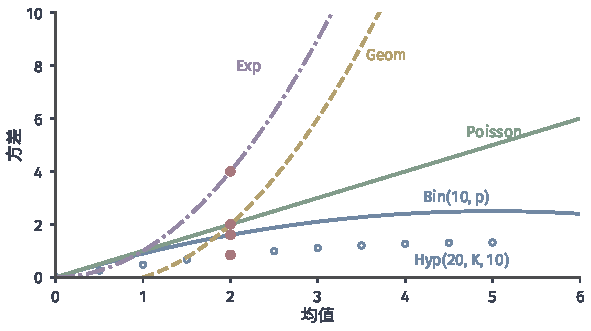
\includegraphics[width=100mm]{figures/07-probability/01-elementary-probability/matplotlib/cdist-mean-variance/figure.pdf}
  \caption{单参数族中方差随均值的变化。$\operatorname{Bin}(10,p)$（蓝线）、$\operatorname{Hyp}(20,K,10)$（蓝色空心点，$K=0,\dots,10$）、$\operatorname{Poisson}$（绿）、$\operatorname{Geom}$（黄，均值不小于$1$）和$\operatorname{Exp}$（紫）。红点是均值为$2$时的方差$0.842$、$1.6$、$2$、$4$，其中$\operatorname{Poisson}(2)$与$\operatorname{Geom}(1/2)$重合于方差$2$。}
  \label{fig:cdist-mean-variance}
\end{BookInlineFigure}

\paragraph{矩的存在与尾部}
表~\ref{tab:cdist-continuous}中只有t分布的矩不全存在。$\nu\leq2$时方差为无穷大，Cauchy分布连期望都没有；这时“均值加减几个标准差”的说法根本无从谈起，只能用中位数和分位数描述位置与离散程度。

即使方差有限，它也不能决定尾部。表~\ref{tab:cdist-tails}把四个方差都为$1$、中心都为$0$的分布放在一起，列出偏离超过$k$个标准差的概率。均匀分布$\operatorname{Unif}(-\sqrt3,\sqrt3)$的支撑有界，超过$\sqrt3$倍标准差的概率就是零；高斯分布的尾部按$\mathrm{e}^{-k^{2}/2}$下降；Laplace分布按$\mathrm{e}^{-\sqrt2k}$下降；$t_3$按幂函数下降。

\begin{BookInlineTable}
  \centering
  \caption{方差为$1$的四种对称分布偏离超过$k$个标准差的概率$\mathbb{P}(\lvert X\rvert>k)$。$t_3$取尺度$1/\sqrt3$。}
  \label{tab:cdist-tails}
  \begin{tabular}{ccccc}
    \toprule
    $k$ & 均匀 & 高斯 & Laplace & $t_3$\\
    \midrule
    $2$ & $0$ & $0.0455$ & $0.0591$ & $0.0405$\\
    $3$ & $0$ & $0.0027$ & $0.0144$ & $0.0138$\\
    $5$ & $0$ & $5.7\times10^{-7}$ & $8.5\times10^{-4}$ & $3.2\times10^{-3}$\\
    \bottomrule
  \end{tabular}
\end{BookInlineTable}

这张表还有一个容易忽略的地方：在$k=2$处，$t_3$的尾概率$0.0405$反而小于高斯的$0.0455$。方差相同时，厚尾分布把更多质量放在中心和极远处，中间一段就要少一些；“尾部更厚”指的是足够远处的行为，并不是在每个阈值上概率都更大。第~\ref{chap:tail-probabilities}章将在只知道均值、方差或更高阶矩时，研究对所有分布都成立的尾概率上界，这些精确值正好用来检验上界的松紧。

\paragraph{边界、特例与极限}
参数取到端点时，模型会退化或变成另一个模型。图~\ref{fig:cdist-family-map}把本章出现过的联系画在一起。实线箭头是本章证明或说明过的构造与极限：$n$个独立Bernoulli变量之和服从二项分布，总体无限增大时超几何趋于二项，$np=\lambda$固定而$n\to\infty$时二项趋于Poisson，步长趋于零时几何等待趋于指数等待，自由度趋于无穷时t密度趋于高斯密度。虚线是族内的特例：$\alpha=1$的Gamma分布是指数分布，$\operatorname{Beta}(1,1)$是均匀分布，$\nu=1$的t分布是Cauchy分布，卡方分布是Gamma分布的子族。

\begin{BookInlineFigure}
  \centering
  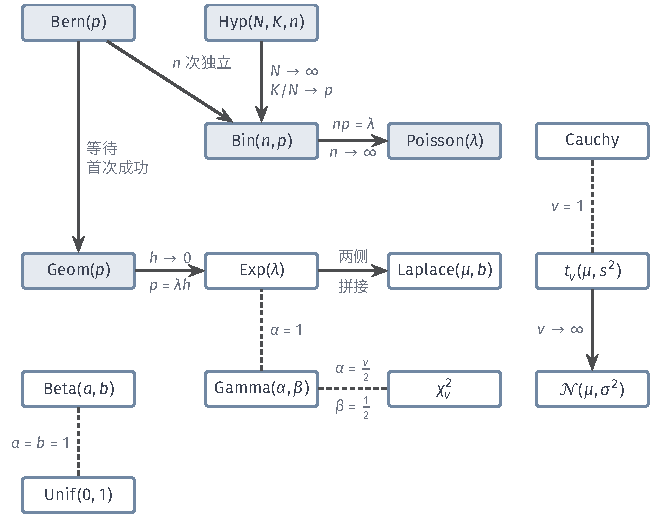
\includegraphics[width=110mm]{figures/07-probability/01-elementary-probability/tikz/cdist-family-map/figure.pdf}
  \caption{本章各一元模型之间的联系。浅蓝框为离散模型，白框为连续模型；实线箭头表示构造或极限，箭头旁注明条件；虚线表示族内的特殊参数值。}
  \label{fig:cdist-family-map}
\end{BookInlineFigure}

每一条极限都附带着近似成立的条件，用近似模型代替原模型时要先核对。二项分布换成Poisson分布，需要机会多而每次稀少，$\operatorname{Bin}(10,0.2)$的零概率就差了近三成；超几何换成二项，需要抽样比例小，否则方差会被高估；t分布换成高斯，在中心附近误差很小，但对任何有限的$\nu$，远处的尾概率都相差数量级。退化的端点（$p=0$或$1$，$n=N$，$K=0$或$N$，$\lambda=0$）则使随机变量成为常数，公式虽然仍可代入，含义要单独理解。

\paragraph{选择的次序}
综合起来，选择一元模型可以按这样的次序检查。先看取值：是计数、等待次数、连续的正值、比例，还是可正可负的误差。再看机制：试验次数是否固定，是否放回，各次是否独立，事件是否稀少。然后看参数的含义：哪个是位置，哪个是尺度，哪个改变形状，率与尺度用的是哪种写法。最后核对需要的矩是否存在、尾部是否合理。只有均值或只有均值和方差相同，不足以让一个模型代替另一个。


\section{本章小结}
\label{sec:cdist-summary}

本章把前两章的分布表示和数值特征落实到十二个可以直接计算的模型上。离散模型都由试验机制推出：一次成败给出Bernoulli分布；固定次数的独立重复给出二项分布；有限总体的不放回抽样给出超几何分布；等待首次成功给出几何分布；机会多、每次稀少的计数，作为二项分布的极限，给出Poisson分布。连续模型则由取值范围和形状要求确定，先验证密度的归一化，再计算矩。

几个计算工具贯穿全章。指示变量把计数写成事件之和，期望由线性性直接得到，不需要独立性；方差要用到两两交事件的概率，独立与否在这里起决定作用，不放回抽样的负牵连带来有限总体修正。尾概率求和处理了取值无穷多的离散变量。Gauss积分、Gamma函数与Beta函数提供了连续模型的归一化常数，分部积分与代换给出各阶矩。

每个公式都带着条件。几何分布要求$p>0$，并且要分清计数是否包含成功的那一次；超几何方差的公式要求$N>1$；Gamma分布有率和尺度两种写法，同一组数字按两种写法理解，期望可以相差好几倍；t分布只有阶数小于$\nu$的矩，$\nu\leq1$时期望不存在，Cauchy分布的对称中心是中位数而不是期望。尺度参数与标准差的比例因分布而异，只有高斯分布的$\sigma$恰为标准差。

模型的比较说明，均值相同甚至均值和方差都相同，也不能让一个模型代替另一个：试验机制、支撑、方差随均值的变化规律和尾部形状都可能不同。方差相同的分布，远处的尾概率可以相差几个数量级。下一章研究这些尾概率：已知完整分布时直接计算，只知道均值、方差或更高阶矩时，能给出怎样的上界，本章的模型将用来检验这些上界的松紧。


\chapter{随机变量的尾概率}
\label{chap:tail-probabilities}

把一枚均匀硬币掷$20$次，正面次数$X$服从$\operatorname{Bin}(20,1/2)$。平均来说正面有$10$次，可是至少$15$次正面的机会有多大？分布完全已知，答案可以直接加出来：把$k=15,\dots,20$六个质量相加，得到约$0.0207$。

换一个处境。一台服务器的响应时间平均为$2$秒，此外我们一无所知。超过$5$秒的请求最多能占多少？这时没有质量表可加，只能问：在所有平均值为$2$的非负分布中，超过$5$的概率最大是多少。答案是一个对所有这些分布同时成立的上界。

这两类问题都关心\emph{尾部}：随机变量越过某个阈值，或者离中心太远的概率。把概率看成总量为一的质量，尾概率就是散落在远处的那一部分质量。它的大小决定了“极端结果”有多常见，也决定了平均值、方差这些数是否存在。

本章先把尾事件写清楚：怎样由分布函数计算单侧与双侧的尾概率，含原子时端点怎样处理，尾概率与期望有什么关系。然后在只知道少量数值特征时依次给出上界：只用非负变量的均值得到Markov不等式，加上方差得到Chebyshev不等式，用更高阶矩和指数矩得到更快衰减的界。每一步都用同一个掷硬币的例子与精确值比较。最后把这些界放在一起评价：各用了多少信息，在哪些阈值上有用，遇到矩不存在的重尾模型时还剩什么。

\section{尾概率}
\label{sec:tail-events}

“至少$15$次正面”“响应超过$5$秒”“测量误差超过$0.1$”，这些事件有一个共同形状：随机变量落在某个阈值的一侧，或者离某个中心至少有给定距离。先把这类事件写成统一的形式，再看已知完整分布时怎样计算它们的概率。

\paragraph{单侧尾事件}
对随机变量$X$和实数$t$，事件$\{X>t\}$与$\{X\geq t\}$说的是$X$落在$t$的右边，事件$\{X<t\}$与$\{X\leq t\}$说的是落在左边。它们的概率都描述质量在一侧的残余，统称尾概率。

\begin{definition}[尾概率]
\label{def:tail-probability}
设$X$是随机变量，$t\in\mathbb{R}$。称
\begin{equation}
 \mathbb{P}(X>t),\qquad \mathbb{P}(X\geq t)
 \label{eq:tail-right}
\end{equation}
为$X$在$t$处的\term{右尾概率}（right tail probability），称$\mathbb{P}(X<t)$与$\mathbb{P}(X\leq t)$为左尾概率，二者统称\term{尾概率}（tail probability）。函数$t\mapsto\mathbb{P}(X>t)$称为$X$的\term{生存函数}（survival function）。
\end{definition}

“生存函数”的名字来自等待时间：若$X$是一个元件的寿命，$\mathbb{P}(X>t)$就是它活过时刻$t$的概率。这个函数从左到右不增，$t$趋于$+\infty$时趋于$0$。它下降得多快，就是本章所说的“尾部有多重”。

\paragraph{由分布函数计算}
分布函数$F_X(t)=\mathbb{P}(X\leq t)$直接给出两种尾概率：
\begin{equation}
 \mathbb{P}(X\leq t)=F_X(t),\qquad \mathbb{P}(X>t)=1-F_X(t).
 \label{eq:tail-from-cdf}
\end{equation}
后一个等式来自$\{X>t\}$是$\{X\leq t\}$的补事件。

带等号的右尾要小心。由第~\ref{chap:random-variables}章，分布函数在每一点有左极限，记作$F_X(t^-)=\lim_{s\to t^-}F_X(s)$，它等于$\mathbb{P}(X<t)$，跳跃高度$F_X(t)-F_X(t^-)$等于$\mathbb{P}(X=t)$。于是$\{X\geq t\}$作为$\{X<t\}$的补事件，概率是
\begin{equation}
 \mathbb{P}(X\geq t)=1-F_X(t^-)=1-F_X(t)+\mathbb{P}(X=t).
 \label{eq:tail-closed}
\end{equation}
只有当$X$在$t$处没有原子，即$\mathbb{P}(X=t)=0$时，才有$\mathbb{P}(X\geq t)=1-F_X(t)$。离散变量在可能取值处恰好有原子，这时把两者混用会差出整整一个点的质量。

\paragraph{贯穿例子}
掷$20$次均匀硬币，正面次数$X\sim\operatorname{Bin}(20,1/2)$，质量为
\[
 p_X(k)=\binom{20}{k}2^{-20},\qquad k=0,1,\dots,20 .
\]
由对称性$p_X(10+j)=p_X(10-j)$，只需列出$k\geq10$的一半。表~\ref{tab:tail-binomial}给出这些组合数，本章所有关于$X$的精确值都由这张表加出来，分母都是$2^{20}=1048576$。

\begin{BookInlineTable}
 \centering
 \caption{$X\sim\operatorname{Bin}(20,1/2)$在$k\geq10$处的组合数$\binom{20}{k}$，质量为$\binom{20}{k}/2^{20}$；$k<10$的部分由$\binom{20}{k}=\binom{20}{20-k}$得到。}
 \label{tab:tail-binomial}
 \begin{tabular}{rrrrrrr}
  \toprule
  $k$ & $10$ & $11$ & $12$ & $13$ & $14$ & $15$\\
  $\binom{20}{k}$ & $184756$ & $167960$ & $125970$ & $77520$ & $38760$ & $15504$\\
  \midrule
  $k$ & $16$ & $17$ & $18$ & $19$ & $20$ & \\
  $\binom{20}{k}$ & $4845$ & $1140$ & $190$ & $20$ & $1$ & \\
  \bottomrule
 \end{tabular}
\end{BookInlineTable}

至少$15$次正面的概率是最后六项之和：
\[
 \mathbb{P}(X\geq15)=\frac{15504+4845+1140+190+20+1}{2^{20}}=\frac{21700}{2^{20}}\approx0.02069 .
\]
严格多于$15$次则去掉$k=15$这一项：
\[
 \mathbb{P}(X>15)=\frac{6196}{2^{20}}\approx0.00591 .
\]
两者相差$p_X(15)=15504/2^{20}\approx0.01479$，比$\mathbb{P}(X>15)$本身还大。按式~\eqref{eq:tail-from-cdf}算出的$1-F_X(15)$是后者，不是前者。

图~\ref{fig:tail-binomial-tail}把这件事画了出来。左图的浅蓝柱是事件$\{X\geq15\}$包含的质量；右图是分布函数在$15$附近的阶梯，$15$处的竖直跳跃正是$p_X(15)$。$F_X(15^-)$取在跳跃下端，$F_X(15)$取在上端，用哪一个取决于端点是否算进尾事件。

\begin{BookInlineFigure}
 \centering
 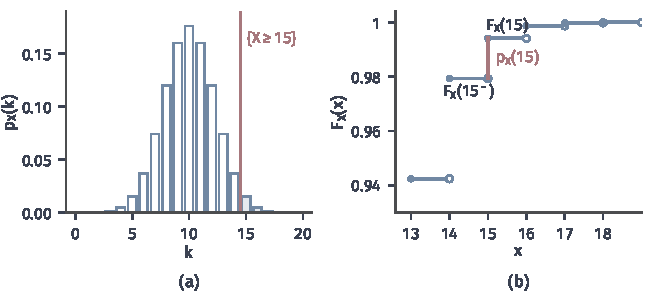
\includegraphics[width=112mm]{figures/07-probability/01-elementary-probability/matplotlib/tail-binomial-tail/figure.pdf}
 \caption{$X\sim\operatorname{Bin}(20,1/2)$的右尾。(a)质量表，浅蓝柱是事件$\{X\geq15\}$的质量，红线是阈值。(b)分布函数在$13$到$19$之间的阶梯，实心点是取到的值，空心点是左极限；红色竖线是$15$处的跳跃，高度为$p_X(15)$。}
 \label{fig:tail-binomial-tail}
\end{BookInlineFigure}

\paragraph{有密度的情形}
若$X$有密度$f_X$，单点概率为零，两种右尾相等，都等于密度在$t$右侧的面积：
\begin{equation}
 \mathbb{P}(X\geq t)=\mathbb{P}(X>t)=\int_t^{\infty}f_X(x)\,\mathrm{d}x .
 \label{eq:tail-density}
\end{equation}
三个模型足以展示尾部的不同衰减方式。$X\sim\operatorname{Exp}(1)$时积分得$\mathbb{P}(X>t)=\mathrm{e}^{-t}$，$t\geq0$。$Z\sim\mathcal{N}(0,1)$时右尾记作
\[
 Q(t)=\mathbb{P}(Z>t)=\int_t^{\infty}\frac{1}{\sqrt{2\pi}}\mathrm{e}^{-x^2/2}\,\mathrm{d}x ,
\]
它没有初等原函数，需要数值积分。常用的几个值是
\[
 Q(1)\approx0.1587,\quad Q(2)\approx0.02275,\quad Q(3)\approx0.00135 .
\]

第三个模型的尾部只按幂次衰减。对$\alpha>0$，在$[1,\infty)$上取密度$f_X(x)=\alpha x^{-\alpha-1}$，积分得
\begin{equation}
 \mathbb{P}(X>t)=\int_t^{\infty}\alpha x^{-\alpha-1}\,\mathrm{d}x=t^{-\alpha},\qquad t\geq1 .
 \label{eq:tail-pareto}
\end{equation}
令$t=1$得总质量为一，所以这确是密度。这个分布称为参数为$\alpha$的\term{Pareto分布}（Pareto distribution），$t<1$时$\mathbb{P}(X>t)=1$。本章用$\alpha=3$作为尾部较重的代表。

图~\ref{fig:tail-decay-shapes}把三条生存函数画在对数纵轴上。指数分布是一条直线，斜率为$-1$；高斯尾部向下弯，越来越陡，因为指数里是$t^2$；Pareto尾部越来越平，在$t=5$处仍有$0.008$，同一处高斯尾部已不到$3\times10^{-7}$。对数坐标把“远处还剩多少质量”的差别放大到了肉眼可见的程度。

\begin{BookInlineFigure}
 \centering
 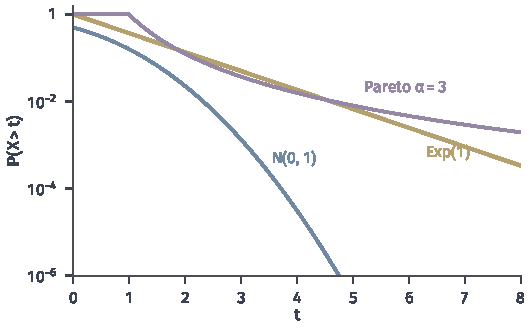
\includegraphics[width=90mm]{figures/07-probability/01-elementary-probability/matplotlib/tail-decay-shapes/figure.pdf}
 \caption{三种右尾，纵轴为对数刻度。蓝线为$\mathcal{N}(0,1)$的$Q(t)$，黄线为$\operatorname{Exp}(1)$的$\mathrm{e}^{-t}$，紫线为$\alpha=3$的Pareto分布的$\min\{1,t^{-3}\}$。}
 \label{fig:tail-decay-shapes}
\end{BookInlineFigure}

\paragraph{偏离中心的双侧事件}
很多时候关心的不是越过某个阈值，而是离某个中心$a$太远，例如测量值偏离真值至少$t$。对$t>0$，事件$\{\lvert X-a\rvert\geq t\}$拆成两个不相交的单侧事件：
\[
 \{\lvert X-a\rvert\geq t\}=\{X\geq a+t\}\cup\{X\leq a-t\} .
\]
两部分不相交，因为$a+t>a-t$。由加法规则和式~\eqref{eq:tail-closed}，
\begin{equation}
 \mathbb{P}(\lvert X-a\rvert\geq t)=1-F_X\bigl((a+t)^-\bigr)+F_X(a-t) .
 \label{eq:tail-two-sided}
\end{equation}
若$X$关于$a$对称，两部分相等，双侧概率是单侧的两倍。贯穿例子关于$10$对称，所以
\[
 \mathbb{P}(\lvert X-10\rvert\geq5)=2\,\mathbb{P}(X\geq15)=\frac{43400}{2^{20}}\approx0.04139 .
\]

分布不对称时两侧必须分开算。取$X\sim\operatorname{Exp}(1)$，均值为$1$，问偏离均值至少$t=0.5$的概率。左侧是$\{X\leq0.5\}$，右侧是$\{X\geq1.5\}$，分别为
\[
 \mathbb{P}(X\leq0.5)=1-\mathrm{e}^{-0.5}\approx0.3935,\qquad \mathbb{P}(X\geq1.5)=\mathrm{e}^{-1.5}\approx0.2231 .
\]
相加得$0.6166$，左侧贡献更大，见图~\ref{fig:tail-two-sided}。若$t\geq1$，左侧事件$\{X\leq1-t\}$要求$X\leq0$，概率为零，只剩右侧$\mathrm{e}^{-(1+t)}$。

\begin{BookInlineFigure}
 \centering
 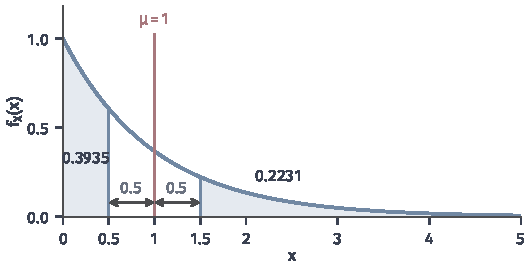
\includegraphics[width=90mm]{figures/07-probability/01-elementary-probability/matplotlib/tail-two-sided/figure.pdf}
 \caption{$X\sim\operatorname{Exp}(1)$偏离均值$\mu=1$至少$0.5$的事件。蓝线为密度，两块浅蓝区域是$\{X\leq0.5\}$与$\{X\geq1.5\}$，数字是各自的面积；红线标出均值。}
 \label{fig:tail-two-sided}
\end{BookInlineFigure}

\paragraph{尾概率与期望}
尾概率与期望之间有一条直接的联系。对非负整数值的变量，把$k\,p_X(k)$写成$k$个$p_X(k)$之和，再按“至少为$j$”重新归组：
\[
 \mathbb{E}[X]=\sum_{k\geq1}\sum_{j=1}^{k}p_X(k)=\sum_{j\geq1}\sum_{k\geq j}p_X(k)=\sum_{j\geq1}\mathbb{P}(X\geq j) .
\]
所有项非负，二重级数可以交换求和次序。对贯穿例子，把$\mathbb{P}(X\geq j)$对$j=1,\dots,20$相加，正好得到$10$。

有密度时，求和换成积分，并可以推广到$X$的函数。下面的\term{尾积分公式}说明期望完全由生存函数决定，后面检查矩与指数矩是否存在时要用它。

\begin{lemma}[尾积分公式]
\label{lem:tail-integral}
设$X\geq0$有密度$f_X$，$g$在$[0,\infty)$上连续可微且不减。则
\begin{equation}
 \mathbb{E}[g(X)]=g(0)+\int_0^{\infty}g'(s)\,\mathbb{P}(X>s)\,\mathrm{d}s ,
 \label{eq:tail-integral}
\end{equation}
两边同时有限或同时为$+\infty$。特别地，取$g(x)=x$与$g(x)=x^p$（$p>0$）得
\begin{equation}
 \mathbb{E}[X]=\int_0^{\infty}\mathbb{P}(X>s)\,\mathrm{d}s,\qquad \mathbb{E}[X^p]=\int_0^{\infty}p\,s^{p-1}\,\mathbb{P}(X>s)\,\mathrm{d}s .
 \label{eq:tail-integral-moments}
\end{equation}
\end{lemma}

\begin{proof}
由微积分基本定理，$g(x)-g(0)=\int_0^xg'(s)\,\mathrm{d}s$。两边乘$f_X(x)$并对$x\geq0$积分，得到
\[
 \mathbb{E}[g(X)]-g(0)=\int_0^{\infty}\Bigl(\int_0^{x}g'(s)\,\mathrm{d}s\Bigr)f_X(x)\,\mathrm{d}x .
\]
被积函数$g'(s)f_X(x)$在区域$0\leq s\leq x$上非负，所以可以交换积分次序，结果有限与否不受影响。交换的依据是非负函数的累次积分定理，可参考\BookChapterRef{chap:integration}{卷四第6章“积分”}；第~\ref{chap:probability-spaces}章会把它统一到概率的语言里。交换后内层对$x$从$s$积到$\infty$：
\[
 \mathbb{E}[g(X)]-g(0)=\int_0^{\infty}g'(s)\Bigl(\int_s^{\infty}f_X(x)\,\mathrm{d}x\Bigr)\mathrm{d}s .
\]
内层积分就是$\mathbb{P}(X>s)$，于是得到式~\eqref{eq:tail-integral}。
\end{proof}

用Pareto分布检验这个公式。$\alpha=3$时生存函数在$[0,1)$上为$1$，在$[1,\infty)$上为$s^{-3}$。代入式~\eqref{eq:tail-integral-moments}的第二式，对$0<p<3$，
\[
 \mathbb{E}[X^p]=\int_0^1p\,s^{p-1}\,\mathrm{d}s+\int_1^{\infty}p\,s^{p-4}\,\mathrm{d}s=1+\frac{p}{3-p}=\frac{3}{3-p} .
\]
$p=1$时得均值$3/2$，$p=2$时得$\mathbb{E}[X^2]=3$。若$p\geq3$，第二个积分发散，$p$阶矩为$+\infty$。尾部$s^{-3}$的衰减速度直接决定了哪些矩存在。

\paragraph{计算与估计}
已知完整分布时，尾概率是一个确定的数，按式~\eqref{eq:tail-closed}或式~\eqref{eq:tail-density}算出即可。反过来给定尾概率的水平去找阈值，就是第~\ref{chap:random-variables}章的分位数。直接计算的困难在于信息：很多时候只知道均值、方差之类的少数数值，或者完整分布虽然存在，却写不出可以求和、积分的形式。

这时能做的是给出\emph{上界}：找一个只依赖已知数值的量，保证所有具有这些数值的分布，其尾概率都不超过它。上界是一种保证，不是估计值；它必须对已知信息允许的最坏分布也成立。下面几节依次增加已知信息，看保证能收紧到什么程度。


\section{Markov不等式}
\label{sec:tail-markov}

回到响应时间。设$X\geq0$，平均$\mathbb{E}[X]=2$秒。有没有可能一半的请求都超过$5$秒？不可能：这一半请求单是自己就给平均值贡献了至少$0.5\times5=2.5$秒，已经超过$2$。这个“远处的质量至少按阈值计入平均”的想法，就是本节的全部内容。

\paragraph{重心的论证}
把分布看成数轴上总量为一的质量，期望是它的重心。质量全在$[0,\infty)$上时，落在$t$右边的那部分质量对重心的贡献至少是“质量乘$t$”；其余质量的贡献至少是$0$。重心又只有$\mathbb{E}[X]$那么远，所以远处的质量不能太多。

\begin{theorem}[Markov不等式]
\label{thm:tail-markov}
设随机变量$X\geq0$，$\mathbb{E}[X]<\infty$。则对每个$t>0$，
\begin{equation}
 \mathbb{P}(X\geq t)\leq\frac{\mathbb{E}[X]}{t} .
 \label{eq:tail-markov}
\end{equation}
\end{theorem}

这个结论称为\term{Markov不等式}（Markov inequality）。证明把“至少贡献$t$”写成两个随机变量之间的比较。

\begin{proof}
考虑示性变量$\mathbf{1}_{\{X\geq t\}}$，它在$X\geq t$时取$1$，否则取$0$。逐个样本点比较$t\,\mathbf{1}_{\{X\geq t\}}$与$X$：若$X\geq t$，左边是$t$，不超过$X$；若$X<t$，左边是$0$，由$X\geq0$也不超过$X$。所以
\[
 t\,\mathbf{1}_{\{X\geq t\}}\leq X .
\]
两边取期望。由期望的保序性和线性性（第~\ref{chap:random-variable-moments}章），以及示性变量的期望就是事件的概率，得到
\[
 t\,\mathbb{P}(X\geq t)\leq\mathbb{E}[X] .
\]
除以$t>0$即得式~\eqref{eq:tail-markov}。
\end{proof}

证明的关键一步是用一个函数从上方压住尾事件的示性函数。图~\ref{fig:tail-dominating}(a)画的就是这一点：蓝色台阶是$\mathbf{1}_{\{x\geq t\}}$，紫色直线是$x/t$，在$x\geq0$上直线处处不低于台阶。取期望后，台阶给出概率，直线给出$\mathbb{E}[X]/t$。另外两个子图是后两节要用的压法，换一个压住台阶的函数，就换一个不等式。

\begin{BookInlineFigure}
 \centering
 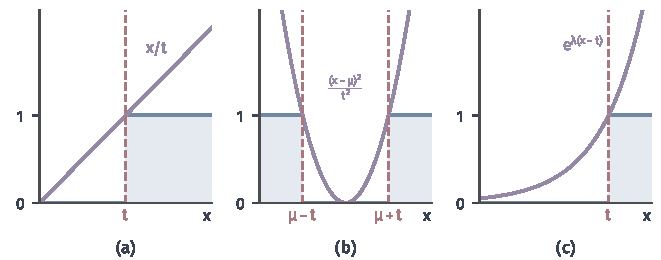
\includegraphics[width=112mm]{figures/07-probability/01-elementary-probability/matplotlib/tail-dominating/figure.pdf}
 \caption{用函数从上方压住尾事件的示性函数。蓝色台阶与浅蓝区域是示性函数，紫线是压住它的函数，红色虚线是阈值。(a)$x\geq0$上的$x/t$。(b)$(x-\mu)^2/t^2$。(c)$\mathrm{e}^{\lambda(x-t)}$，$\lambda>0$。}
 \label{fig:tail-dominating}
\end{BookInlineFigure}

\paragraph{搬动质量的图景}
同一个证明还可以看成搬动质量。把$[0,t)$里的质量全部搬到$0$，把$[t,\infty)$里的质量全部搬到$t$。每块质量只向左移动，重心只会左移；搬完以后，$t$处的质量仍是$\mathbb{P}(X\geq t)$，新重心是$t\,\mathbb{P}(X\geq t)$。于是新重心不超过原重心，这正是$t\,\mathbb{P}(X\geq t)\leq\mathbb{E}[X]$。

图~\ref{fig:tail-markov-mass}用一个六点分布演示。上排质量依次为$0.15$、$0.25$、$0.20$、$0.15$、$0.15$、$0.10$，位于$1$、$2$、$3$、$4$、$6$、$8$，重心为
\[
 \mu=0.15+0.5+0.6+0.6+0.9+0.8=3.55 .
\]
取$t=5$，右边有质量$0.25$。搬动后下排只剩$0$处的$0.75$和$5$处的$0.25$，重心变为$5\times0.25=1.25\leq3.55$。

\begin{BookInlineFigure}
 \centering
 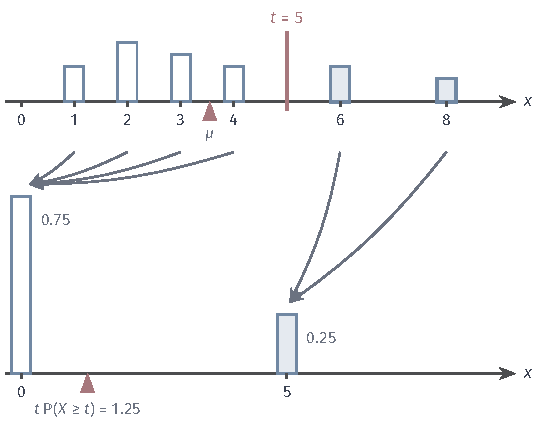
\includegraphics[width=92mm]{figures/07-probability/01-elementary-probability/tikz/tail-markov-mass/figure.pdf}
 \caption{Markov不等式的搬动质量论证。上排是原分布，浅蓝柱是$\{X\geq5\}$的质量，红线是阈值$t=5$，红三角是重心$\mu=3.55$。灰色箭头把$t$左边的质量搬到$0$，把右边的质量搬到$t$。下排是搬动后的两点分布，重心降为$t\,\mathbb{P}(X\geq t)=1.25$。}
 \label{fig:tail-markov-mass}
\end{BookInlineFigure}

\paragraph{面积的图景}
第三种看法用尾积分公式。由式~\eqref{eq:tail-integral-moments}，$\mathbb{E}[X]$是生存函数$s\mapsto\mathbb{P}(X>s)$下方的面积。对$0\leq s<t$，有$\{X\geq t\}\subseteq\{X>s\}$，所以生存函数在$[0,t)$上不低于$\mathbb{P}(X\geq t)$。宽为$t$、高为$\mathbb{P}(X\geq t)$的矩形整个落在曲线下方，面积不超过总面积。

图~\ref{fig:tail-layer-cake}取$X\sim\operatorname{Exp}(1)$与$t=2$。曲线下总面积是$\mu=1$，黄色矩形面积是$2\mathrm{e}^{-2}\approx0.271$。矩形之外的面积就是Markov不等式没有用上的部分：$t$左边曲线高出矩形的那一块，以及$t$右边的整个尾巴。

\begin{BookInlineFigure}
 \centering
 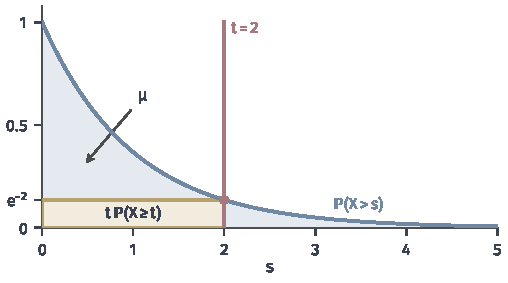
\includegraphics[width=86mm]{figures/07-probability/01-elementary-probability/matplotlib/tail-layer-cake/figure.pdf}
 \caption{$X\sim\operatorname{Exp}(1)$的生存函数（蓝线）。浅蓝区域面积等于$\mu=\mathbb{E}[X]=1$；黄色矩形宽$t=2$、高$\mathbb{P}(X\geq2)=\mathrm{e}^{-2}$，落在曲线下方，所以$t\,\mathbb{P}(X\geq t)\leq\mu$。}
 \label{fig:tail-layer-cake}
\end{BookInlineFigure}

\paragraph{条件的作用}
定理有三个条件，每一个都不能随便去掉。

第一是$X\geq0$。若允许负值，正负质量可以互相抵消，均值不再约束远处的质量。设$X$以各$1/2$的概率取$-100$和$100$，则$\mathbb{E}[X]=0$，但$\mathbb{P}(X\geq1)=1/2$，而式~\eqref{eq:tail-markov}的右边是$0$。证明中失效的一步正是$X<t$时“$0\leq X$”。

第二是$\mathbb{E}[X]<\infty$。若期望为$+\infty$，不等式右边是$+\infty$，仍然成立但不提供任何信息。第三是$t>0$：$t\leq0$时$\{X\geq t\}$是必然事件，概率为$1$，也无需估计。

\paragraph{这个界不能再改进}
Markov不等式只用到均值。它会不会只是证明粗糙，换一种论证就能更紧？答案是否定的：在“非负、均值为$\mu$”这一信息下，它已经是最好的保证。

\begin{theorem}[Markov界的最优性]
\label{thm:tail-markov-sharp}
设$\mu>0$，$t>0$。在所有满足$X\geq0$、$\mathbb{E}[X]=\mu$的随机变量中，$\mathbb{P}(X\geq t)$的最大值为
\begin{equation}
 \sup\,\mathbb{P}(X\geq t)=\min\Bigl\{1,\frac{\mu}{t}\Bigr\} .
 \label{eq:tail-markov-sharp}
\end{equation}
\end{theorem}

\begin{proof}
由Markov不等式和概率不超过$1$，每个这样的$X$都满足$\mathbb{P}(X\geq t)\leq\min\{1,\mu/t\}$。只需构造达到它的分布。

若$\mu\leq t$，令$X$以概率$\mu/t$取$t$，以概率$1-\mu/t$取$0$。它非负，均值为$t\cdot\mu/t=\mu$，并且$\mathbb{P}(X\geq t)=\mu/t$。

若$\mu>t$，令$X$恒等于$\mu$。它的均值是$\mu$，并且$\mathbb{P}(X\geq t)=1$。
\end{proof}

两点分布正是搬动质量后的形状：质量只放在$0$和$t$两处，没有一点“浪费”在比$t$更远的地方，也没有放在$0$与$t$之间。任何具体分布只要在这两种方式上偏离两点分布，它的尾概率就严格小于$\mu/t$。

\paragraph{与精确值比较}
保证与具体模型的实际尾概率可以差得很远。贯穿例子中$\mathbb{E}[X]=10$，Markov不等式给出
\[
 \mathbb{P}(X\geq15)\leq\frac{10}{15}=\frac23\approx0.667 ,
\]
而精确值是$0.0207$，相差三十多倍。指数分布$X\sim\operatorname{Exp}(1)$的均值为$1$，Markov界是$1/t$，精确值是$\mathrm{e}^{-t}$：$t=5$时前者是$0.2$，后者是$0.0067$。

图~\ref{fig:tail-markov-compare}在对数纵轴上画出两组比较。精确尾部在两个例子中都下降得飞快，Markov界只按$1/t$缓慢下降。差距的来源并不是证明不精细，而是信息太少：界必须同时照顾到两点分布那样的极端情形。要得到更好的界，只能使用更多关于分布的信息。

\begin{BookInlineFigure}
 \centering
 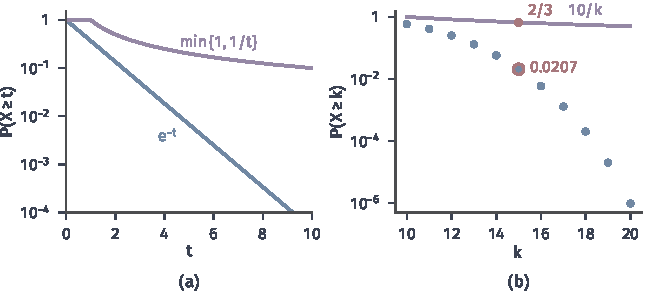
\includegraphics[width=112mm]{figures/07-probability/01-elementary-probability/matplotlib/tail-markov-compare/figure.pdf}
 \caption{Markov界（紫线）与精确尾概率（蓝色），纵轴为对数刻度。(a)$X\sim\operatorname{Exp}(1)$，精确值$\mathrm{e}^{-t}$。(b)$X\sim\operatorname{Bin}(20,1/2)$，蓝点为$\mathbb{P}(X\geq k)$，紫线为$10/k$，红色标出$k=15$处的$2/3$与$0.0207$。}
 \label{fig:tail-markov-compare}
\end{BookInlineFigure}

\paragraph{一般形式}
压住示性函数的不必是直线。只要函数$g$非负且不减，事件$\{X\geq t\}$就包含在$\{g(X)\geq g(t)\}$之中，对$g(X)$用Markov不等式即可。下面的形式是后面三节的共同出发点。

\begin{lemma}[Markov不等式的一般形式]
\label{lem:tail-markov-general}
设$g$是$\mathbb{R}$上的非负不减函数，$t$满足$g(t)>0$，且$\mathbb{E}[g(X)]<\infty$。则
\begin{equation}
 \mathbb{P}(X\geq t)\leq\frac{\mathbb{E}[g(X)]}{g(t)} .
 \label{eq:tail-markov-general}
\end{equation}
\end{lemma}

\begin{proof}
若$X\geq t$，由$g$不减得$g(X)\geq g(t)$，所以$\{X\geq t\}\subseteq\{g(X)\geq g(t)\}$，前者的概率不超过后者。$g(X)$非负，期望有限，$g(t)>0$，对它用定理~\ref{thm:tail-markov}：
\[
 \mathbb{P}(X\geq t)\leq\mathbb{P}\bigl(g(X)\geq g(t)\bigr)\leq\frac{\mathbb{E}[g(X)]}{g(t)} .
\]
这就是式~\eqref{eq:tail-markov-general}。
\end{proof}

这里不再要求$X\geq0$，非负性转移给了$g$。选择$g$就是选择要用分布的哪一项信息：对非负变量$\lvert X-a\rvert$取$g(s)=\max\{s,0\}^p$，用的是$p$阶绝对矩；对$X$本身取$g(x)=\mathrm{e}^{\lambda x}$，用的是指数矩。$g$在远处增长越快，远处的质量在$\mathbb{E}[g(X)]$里被放得越大，界就可能衰减得越快；代价是$\mathbb{E}[g(X)]$有限的要求越强。


\section{Chebyshev不等式}
\label{sec:tail-chebyshev}

测量值会偏高也会偏低，我们常关心的是它离均值有多远，而不是越过哪一个固定阈值。偏离$X-\mu$可正可负，Markov不等式不能直接用；取绝对值或平方以后才非负。平方的好处是它的期望正是方差，一个最常知道的数。

\paragraph{转动惯量的论证}
继续把分布看成质量。方差$\operatorname{Var}(X)=\mathbb{E}[(X-\mu)^2]$是质量绕重心$\mu$的转动惯量：每块质量按到重心距离的平方加权。离重心至少$t$的质量，对转动惯量的贡献至少是“质量乘$t^2$”。转动惯量只有$\sigma^2$那么大，所以远离重心的质量至多是$\sigma^2/t^2$。

\begin{theorem}[Chebyshev不等式]
\label{thm:tail-chebyshev}
设$X$的方差有限，记$\mu=\mathbb{E}[X]$，$\sigma^2=\operatorname{Var}(X)$。则对每个$t>0$，
\begin{equation}
 \mathbb{P}(\lvert X-\mu\rvert\geq t)\leq\frac{\sigma^2}{t^2} .
 \label{eq:tail-chebyshev}
\end{equation}
\end{theorem}

这个结论称为\term{Chebyshev不等式}（Chebyshev inequality）。

\begin{proof}
因为$t>0$，两个非负数$\lvert X-\mu\rvert$与$t$的大小关系在平方后保持不变，所以两个事件相同：
\[
 \{\lvert X-\mu\rvert\geq t\}=\{(X-\mu)^2\geq t^2\} .
\]
$(X-\mu)^2$是非负随机变量，期望为$\sigma^2<\infty$。对它在阈值$t^2>0$处用定理~\ref{thm:tail-markov}，得到
\[
 \mathbb{P}\bigl((X-\mu)^2\geq t^2\bigr)\leq\frac{\mathbb{E}[(X-\mu)^2]}{t^2}=\frac{\sigma^2}{t^2} .
\]
两个事件相同，这就是式~\eqref{eq:tail-chebyshev}。
\end{proof}

压住示性函数的函数这次是抛物线，见图~\ref{fig:tail-dominating}(b)：$(x-\mu)^2/t^2$在$\lvert x-\mu\rvert\geq t$时不小于$1$，在其他地方不小于$0$。与直线相比，抛物线在两侧同时向上，所以一次控制住两个方向的偏离。

\paragraph{以标准差为单位}
当$\sigma>0$时，取$t=k\sigma$，式~\eqref{eq:tail-chebyshev}成为
\begin{equation}
 \mathbb{P}(\lvert X-\mu\rvert\geq k\sigma)\leq\frac{1}{k^2},\qquad k>0 .
 \label{eq:tail-chebyshev-k}
\end{equation}
它对每个方差有限的分布都成立。取$k=2$和$k=3$，任何这样的分布至少有$75\%$的质量落在均值两侧两个标准差以内，至少有$1-1/9\approx88.9\%$落在三个标准差以内。$k\leq1$时右边不小于$1$，不提供信息。

\paragraph{条件的作用}
定理只要求方差有限，不要求非负，也不要求对称。方差无穷时右边是$+\infty$，不等式没有内容；第~\ref{chap:common-distributions}章中自由度$\nu\leq2$的t分布就是这样，这时只能改用阶数更低的矩，见下一节。式~\eqref{eq:tail-chebyshev}控制的是双侧事件。单侧事件$\{X\geq\mu+t\}$包含在其中，所以同一个界也适用于单侧，只是不一定紧。

\paragraph{这个界同样不能再改进}
与Markov不等式一样，只知道均值和方差时，$\sigma^2/t^2$已经是最好的保证。设$0<\sigma\leq t$，构造三点分布：
\[
 \mathbb{P}(X=\mu-t)=\mathbb{P}(X=\mu+t)=\frac{\sigma^2}{2t^2},\qquad \mathbb{P}(X=\mu)=1-\frac{\sigma^2}{t^2} .
\]
它关于$\mu$对称，所以均值为$\mu$。偏离为$\pm t$的两点各贡献$t^2\cdot\sigma^2/(2t^2)$，合起来方差为
\[
 \operatorname{Var}(X)=2\cdot t^2\cdot\frac{\sigma^2}{2t^2}=\sigma^2 ,
\]
而$\mathbb{P}(\lvert X-\mu\rvert\geq t)=\sigma^2/t^2$，等号成立。

这个分布的形状与Markov的两点分布同出一辙：远处的质量恰好放在距离$t$处，一点也不再往外放，其余质量全部堆在中心，不贡献转动惯量。图~\ref{fig:tail-chebyshev-extremal}取$\mu=0$，$\sigma=1$，$t=2$，三点的质量为$1/8,3/4,1/8$，双侧尾概率是$1/4$；同样均值和方差的标准高斯分布，双侧尾概率只有$0.0455$。

\begin{BookInlineFigure}
 \centering
 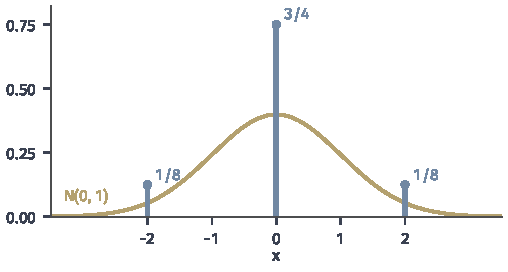
\includegraphics[width=86mm]{figures/07-probability/01-elementary-probability/matplotlib/tail-chebyshev-extremal/figure.pdf}
 \caption{使Chebyshev不等式取等号的三点分布（蓝色竖线，$\mu=0$，$\sigma=1$，$t=2$），质量$1/8,3/4,1/8$位于$-2,0,2$。黄线是均值、方差相同的$\mathcal{N}(0,1)$密度。}
 \label{fig:tail-chebyshev-extremal}
\end{BookInlineFigure}

\paragraph{与精确值比较}
由第~\ref{chap:common-distributions}章，贯穿例子的方差是$20\cdot\frac12\cdot\frac12=5$。取$t=5$，
\[
 \mathbb{P}(\lvert X-10\rvert\geq5)\leq\frac{5}{25}=0.2 .
\]
精确值是$0.0414$，界大了约五倍。单侧事件$\{X\geq15\}$也得到上界$0.2$，比Markov不等式的$2/3$好得多。改进来自两项新信息：方差告诉我们分布有多分散，均值作为中心使界只依赖偏离而不依赖原点的位置。

其他模型上可以看到同样的差距。对$Z\sim\mathcal{N}(0,1)$，
\[
 k=2:\ \tfrac14\ \text{对}\ 0.0455,\qquad k=3:\ \tfrac19\approx0.111\ \text{对}\ 0.0027 .
\]
对$X\sim\operatorname{Unif}(0,1)$，$\mu=1/2$，$\sigma^2=1/12$。$0<t\leq1/2$时精确值是$\mathbb{P}(\lvert X-1/2\rvert\geq t)=1-2t$。取$t=0.4$，精确值为$0.2$，界为$1/(12\times0.16)\approx0.521$。$t>1/2$时精确值是$0$，界却始终为正：Chebyshev不等式不知道分布的取值范围有界。

\paragraph{均值和方差不能决定尾部}
上面的比较说明，均值和方差相同的分布，尾部可以完全不同。图~\ref{fig:tail-same-variance}画出五个均值为$0$、方差为$1$的分布的双侧尾概率$\mathbb{P}(\lvert X\rvert\geq k)$：$[-\sqrt3,\sqrt3]$上的均匀分布，标准高斯分布，尺度为$1/\sqrt2$的Laplace分布，以及以各$1/2$概率取$\pm1$的两点分布。在$k=2$处，五个值分别是
\[
 0,\qquad 0.0455,\qquad \mathrm{e}^{-2\sqrt2}\approx0.0591,\qquad 0,\qquad \tfrac14 ,
\]
最后一个属于该处的三点极端分布。紫色曲线$1/k^2$是所有这些曲线的包络。

\begin{BookInlineFigure}
 \centering
 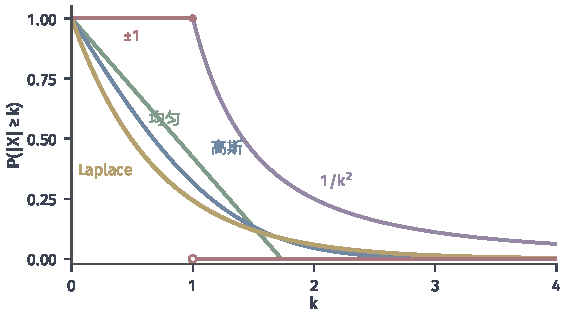
\includegraphics[width=96mm]{figures/07-probability/01-elementary-probability/matplotlib/tail-same-variance/figure.pdf}
 \caption{均值为$0$、方差为$1$的几个分布的双侧尾概率$\mathbb{P}(\lvert X\rvert\geq k)$。绿线为$[-\sqrt3,\sqrt3]$上的均匀分布，蓝线为$\mathcal{N}(0,1)$，黄线为尺度$1/\sqrt2$的Laplace分布，红线为取$\pm1$的两点分布，紫线为Chebyshev界$\min\{1,1/k^2\}$。}
 \label{fig:tail-same-variance}
\end{BookInlineFigure}

包络之下，曲线的形状由均值和方差之外的信息决定：均匀分布在$\sqrt3$处截断，两点分布在$1$处一下跳到零，Laplace分布的尾部比高斯分布更重。从$1/k^2$出发要把界进一步压低，就得知道分布在远处的更多情况，下一节用更高阶的矩来提供这样的信息。


\section{高阶矩上界}
\label{sec:tail-higher-moments}

Chebyshev不等式用平方给远处的质量加权。若把平方换成四次方、六次方，远处的质量在期望里被放得更大，同样大小的矩就迫使远处的质量更少。代价也很明显：要知道更高阶的矩，并且它要有限。

\paragraph{一般的矩上界}
设$a$是任意给定的中心，不必是均值。对非负变量$\lvert X-a\rvert$和$p>0$，函数$s\mapsto s^p$在$[0,\infty)$上严格增，所以对$t>0$，“偏离至少$t$”与“偏离的$p$次方至少$t^p$”是同一个事件。

\begin{theorem}[矩上界]
\label{thm:tail-moment}
设$p>0$，$a\in\mathbb{R}$，且$\mathbb{E}\lvert X-a\rvert^p<\infty$。则对每个$t>0$，
\begin{equation}
 \mathbb{P}(\lvert X-a\rvert\geq t)\leq\frac{\mathbb{E}\lvert X-a\rvert^p}{t^p} .
 \label{eq:tail-moment}
\end{equation}
\end{theorem}

\begin{proof}
因为$t>0$，$p>0$，幂函数$s\mapsto s^p$在$[0,\infty)$上严格增，所以$\lvert X-a\rvert\geq t$当且仅当$\lvert X-a\rvert^p\geq t^p$。$\lvert X-a\rvert^p$非负，期望有限，对它在阈值$t^p>0$处用定理~\ref{thm:tail-markov}：
\[
 \mathbb{P}(\lvert X-a\rvert\geq t)=\mathbb{P}\bigl(\lvert X-a\rvert^p\geq t^p\bigr)\leq\frac{\mathbb{E}\lvert X-a\rvert^p}{t^p} .
\]
这就是式~\eqref{eq:tail-moment}。
\end{proof}

式~\eqref{eq:tail-moment}称为\term{矩上界}（moment bound）。$p=2$、$a=\mu$时它就是Chebyshev不等式；$p=1$时它用的是平均绝对偏离；$p$也可以取非整数，例如$0<p<1$，这在均值都不存在时仍然可用。界按$t^{-p}$衰减，阶数越高，远处衰减越快。

\paragraph{存在条件随阶数加强}
由第~\ref{chap:random-variable-moments}章，$0<p<q$时，$q$阶绝对矩有限蕴含$p$阶绝对矩有限，反之不然。所以使用更高阶的矩是在假设更多。Pareto分布把这一点表现得很清楚：$\alpha=3$时，由第~\ref{sec:tail-events}节的计算，
\[
 \mathbb{E}[X^p]=\frac{3}{3-p},\qquad 0<p<3 ,
\]
$p\geq3$时为$+\infty$。阶数趋于$3$时矩本身趋于无穷，界$3/((3-p)t^p)$的系数随之变大。同样，自由度为$\nu$的t分布只有$p<\nu$阶的绝对矩有限。

\paragraph{贯穿例子的四阶与六阶矩}
对$X\sim\operatorname{Bin}(20,1/2)$，取中心$a=10$。由对称性，$p$阶中心绝对矩是
\[
 m_p=\mathbb{E}\lvert X-10\rvert^p=\frac{2}{2^{20}}\sum_{j=1}^{10}\binom{20}{10+j}j^p .
\]
用表~\ref{tab:tail-binomial}逐项相乘。$p=2$时十项之和是$2621440$，于是$m_2=5$，与方差一致。$p=4$时十项依次为
\[
 \begin{gathered}
 167960,\ 2015520,\ 6279120,\ 9922560,\ 9690000,\\
 6279120,\ 2737140,\ 778240,\ 131220,\ 10000,
 \end{gathered}
\]
和为$38010880$。$p=6$时同样相加，和为$887357440$。乘以$2/2^{20}$，得到
\[
 m_2=5,\qquad m_4=72.5,\qquad m_6=1692.5 .
\]

在$t=5$处比较三个界：
\[
 \frac{m_2}{5^2}=0.2,\qquad \frac{m_4}{5^4}=0.116,\qquad \frac{m_6}{5^6}\approx0.108 .
\]
阶数越高越接近精确值$0.0414$。但在$t=3$处情况相反：
\[
 \frac{m_2}{3^2}\approx0.556,\qquad \frac{m_4}{3^4}\approx0.895,\qquad \frac{m_6}{3^6}\approx2.32 .
\]
六阶的界大于$1$，毫无用处，二阶的界反而最好。

\paragraph{高阶不一定更紧}
原因在于矩把\emph{所有}偏离都按$p$次方加权。偏离小于$t$的质量在$\lvert x-a\rvert^p/t^p$中被压小，偏离大于$t$的质量被放大。$t$较小时，大量质量的偏离与$t$相当或更大，高阶矩被它们放大得很厉害；$t$较大时，远处的质量很少，高阶矩被放大的部分有限，而$t^p$增长得更快。

两个界的交点可以直接解出。四阶界小于二阶界，当且仅当$m_4/t^4<m_2/t^2$，即
\[
 t^2>\frac{m_4}{m_2}=\frac{72.5}{5}=14.5,\qquad t>3.81 .
\]
同理，六阶界小于四阶界当且仅当$t^2>m_6/m_4\approx23.3$，即$t>4.83$。图~\ref{fig:tail-binomial-moment-bounds}显示了这种依次接替：每一阶的界在某个阈值以后才成为最好的。

\begin{BookInlineFigure}
 \centering
 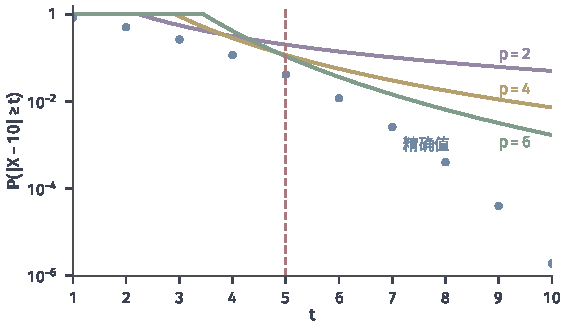
\includegraphics[width=96mm]{figures/07-probability/01-elementary-probability/matplotlib/tail-binomial-moment-bounds/figure.pdf}
 \caption{$X\sim\operatorname{Bin}(20,1/2)$的双侧尾概率$\mathbb{P}(\lvert X-10\rvert\geq t)$（蓝点）与矩上界$\min\{1,m_p/t^p\}$：紫线$p=2$，黄线$p=4$，绿线$p=6$。纵轴为对数刻度，红色虚线标出$t=5$。}
 \label{fig:tail-binomial-moment-bounds}
\end{BookInlineFigure}

\paragraph{给定阈值时选择阶数}
既然没有一个阶数处处最好，自然的做法是对给定的$t$，在所有可用的阶数中取最小的界。标准高斯分布的各阶矩都有限，可以把这件事算到底。记$\varphi(x)=\mathrm{e}^{-x^2/2}/\sqrt{2\pi}$，它满足$\varphi'(x)=-x\varphi(x)$。对$p\geq0$分部积分，边界项因$\varphi$衰减极快而为零，得到
\[
 \mathbb{E}[Z^{p+2}]=\int_{-\infty}^{\infty}x^{p+1}\cdot x\varphi(x)\,\mathrm{d}x=(p+1)\int_{-\infty}^{\infty}x^{p}\varphi(x)\,\mathrm{d}x=(p+1)\,\mathbb{E}[Z^p] .
\]
从$\mathbb{E}[Z^0]=1$出发，偶数阶矩为
\[
 \mathbb{E}[Z^{p}]=(p-1)(p-3)\cdots3\cdot1,\qquad p=2,4,6,\dots .
\]因此从$p$阶换到$p+2$阶，界乘上因子
\[
 \frac{\mathbb{E}[Z^{p+2}]/t^{p+2}}{\mathbb{E}[Z^p]/t^p}=\frac{p+1}{t^2} .
\]
只要$p+1<t^2$，提高阶数就让界变小；一旦$p+1>t^2$，再提高就变大。

$t=2$时$t^2=4$，从$p=2$到$p=4$乘$3/4$，再到$p=6$乘$5/4$，所以最好的偶数阶是$p=4$，界为$3/16=0.1875$。$t=3$时$t^2=9$，从$p=6$到$p=8$乘$7/9$，从$p=8$到$p=10$乘$9/9=1$，界在$p=8$和$p=10$处同为
\[
 \frac{\mathbb{E}[Z^8]}{3^8}=\frac{105}{6561}\approx0.0160 .
\]
奇数阶的绝对矩也可以计算，$p=9$时略小，约为$0.0156$；精确值是$2Q(3)\approx0.0027$。

图~\ref{fig:tail-normal-moment-order}把界作为阶数的函数画出来：曲线先降后升，最低点随$t$右移。最优阶数大约是$t^2$，阈值越远，越要用高阶矩。若只允许用某个固定阶数$p$，界只能按$t^{-p}$衰减，而高斯尾部比任何幂次都衰减得快。要跟上这种衰减，就需要把各阶矩一起利用，这正是下一节指数矩的作用。

\begin{BookInlineFigure}
 \centering
 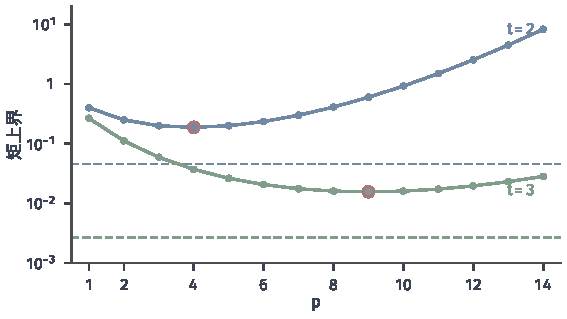
\includegraphics[width=96mm]{figures/07-probability/01-elementary-probability/matplotlib/tail-normal-moment-order/figure.pdf}
 \caption{$Z\sim\mathcal{N}(0,1)$的矩上界$\mathbb{E}\lvert Z\rvert^p/t^p$随阶数$p$的变化，纵轴为对数刻度。蓝色为$t=2$，绿色为$t=3$，红圈是整数阶中的最小值，同色虚线是精确值$\mathbb{P}(\lvert Z\rvert\geq t)$。}
 \label{fig:tail-normal-moment-order}
\end{BookInlineFigure}


\section{指数矩上界}
\label{sec:tail-exponential-moments}

上一节看到，对高斯分布，阈值越远就要用越高阶的矩，而每次都要在许多阶之间挑选。能否一次把所有阶的矩都用上？指数函数的幂级数
\[
 \mathrm{e}^{\lambda x}=\sum_{k\geq0}\frac{\lambda^kx^k}{k!}
\]
恰好把各阶幂次按权重$\lambda^k/k!$加在一起。用$\mathrm{e}^{\lambda x}$去压尾事件的示性函数，得到的界只依赖一个期望。

\paragraph{矩母函数}
先给这个期望一个名字。它对有些$\lambda$有限，对有些$\lambda$可能是$+\infty$，所以同时记录它在哪里有限。

\begin{definition}[矩母函数]
\label{def:tail-mgf}
随机变量$X$的\term{矩母函数}（moment generating function）是
\begin{equation}
 M_X(\lambda)=\mathbb{E}\bigl[\mathrm{e}^{\lambda X}\bigr],\qquad \lambda\in\mathbb{R},
 \label{eq:tail-mgf}
\end{equation}
其中$\mathrm{e}^{\lambda X}>0$，期望总有定义，取值在$(0,+\infty]$中。
\end{definition}

总有$M_X(0)=1$。若$M_X(\lambda)$在$0$附近有限，把$\mathrm{e}^{\lambda X}$按幂级数展开并逐项取期望，$\lambda^k$的系数正是$\mathbb{E}[X^k]/k!$，这就是“矩母”这个名字的来历。逐项取期望的合理性以及矩母函数怎样识别分布，在第~\ref{chap:weak-convergence-of-distributions}章讨论；本节只把$M_X(\lambda)$当作一个可以计算的期望来用。

\paragraph{指数矩上界}
函数$x\mapsto\mathrm{e}^{\lambda x}$在$\lambda>0$时正且严格增，满足引理~\ref{lem:tail-markov-general}的全部条件，并且不要求$X$非负。

\begin{theorem}[指数矩上界]
\label{thm:tail-chernoff}
设$\lambda>0$，$M_X(\lambda)<\infty$。则对每个$t\in\mathbb{R}$，
\begin{equation}
 \mathbb{P}(X\geq t)\leq\mathrm{e}^{-\lambda t}M_X(\lambda) .
 \label{eq:tail-chernoff-lambda}
\end{equation}
因而
\begin{equation}
 \mathbb{P}(X\geq t)\leq\inf_{\lambda>0}\mathrm{e}^{-\lambda t}M_X(\lambda) ,
 \label{eq:tail-chernoff}
\end{equation}
其中$M_X(\lambda)=+\infty$的$\lambda$不起作用。
\end{theorem}

\begin{proof}
在引理~\ref{lem:tail-markov-general}中取$g(x)=\mathrm{e}^{\lambda x}$。它非负、不减，$g(t)=\mathrm{e}^{\lambda t}>0$，$\mathbb{E}[g(X)]=M_X(\lambda)<\infty$，所以
\[
 \mathbb{P}(X\geq t)\leq\frac{M_X(\lambda)}{\mathrm{e}^{\lambda t}}=\mathrm{e}^{-\lambda t}M_X(\lambda) .
\]
左边不依赖$\lambda$，对所有使右边有限的$\lambda>0$取下确界，得到式~\eqref{eq:tail-chernoff}。
\end{proof}

式~\eqref{eq:tail-chernoff}称为\term{Chernoff界}（Chernoff bound）。图~\ref{fig:tail-dominating}(c)是它的压法：$\mathrm{e}^{\lambda(x-t)}$在$x\geq t$时不小于$1$，在$x<t$时为正。$\lambda$控制这条曲线的形状：$\lambda$大时曲线在$t$左边迅速趋于零，把近处的质量压得很小，但在$t$右边陡峭上升，把远处的质量放得很大；$\lambda$小时正好相反。最优的$\lambda$在两者之间折中。

取对数可以把式~\eqref{eq:tail-chernoff}写成指数形式。记$\psi_X(\lambda)=\ln M_X(\lambda)$，则
\begin{equation}
 \mathbb{P}(X\geq t)\leq\exp\Bigl(-\sup_{\lambda>0}\bigl(\lambda t-\psi_X(\lambda)\bigr)\Bigr) .
 \label{eq:tail-chernoff-exponent}
\end{equation}
在下面的例子中，$\lambda t-\psi_X(\lambda)$都可以求导找到最大点。

\paragraph{高斯分布}
先计算$Z\sim\mathcal{N}(0,1)$的矩母函数。把指数部分配方，$\lambda x-x^2/2=\lambda^2/2-(x-\lambda)^2/2$，于是
\[
 M_Z(\lambda)=\mathrm{e}^{\lambda^2/2}\int_{-\infty}^{\infty}\frac{1}{\sqrt{2\pi}}\mathrm{e}^{-(x-\lambda)^2/2}\,\mathrm{d}x=\mathrm{e}^{\lambda^2/2} .
\]
最后的积分是平移后的高斯密度，等于$1$。它对一切实数$\lambda$有限。

代入式~\eqref{eq:tail-chernoff-lambda}，对$t>0$，
\[
 \mathbb{P}(Z\geq t)\leq\mathrm{e}^{-\lambda t+\lambda^2/2} .
\]
指数$-\lambda t+\lambda^2/2$是$\lambda$的二次函数，在$\lambda=t$处取最小值$-t^2/2$。所以
\begin{equation}
 \mathbb{P}(Z\geq t)\leq\mathrm{e}^{-t^2/2},\qquad t>0 .
 \label{eq:tail-gauss-chernoff}
\end{equation}
对$X\sim\mathcal{N}(\mu,\sigma^2)$，写$X=\mu+\sigma Z$，事件$\{X-\mu\geq t\}$就是$\{Z\geq t/\sigma\}$，得到
\[
 \mathbb{P}(X-\mu\geq t)\leq\mathrm{e}^{-t^2/(2\sigma^2)},\qquad t>0 .
\]

图~\ref{fig:tail-chernoff-lambda}(b)画出$t=1,2,3$时的函数$\lambda\mapsto\mathrm{e}^{-\lambda t+\lambda^2/2}$，红点是最小点$\lambda=t$。三个最小值与精确值的对比是
\[
 \begin{gathered}
 t=1:\ 0.607\ \text{对}\ 0.1587,\qquad t=2:\ 0.135\ \text{对}\ 0.0228,\\
 t=3:\ 0.0111\ \text{对}\ 0.00135 .
 \end{gathered}
\]
精确值与上界之比依次约为$0.26$、$0.17$、$0.12$，变化缓慢；起主导作用的因子$\mathrm{e}^{-t^2/2}$被界完整地抓住了。与之相比，Chebyshev界$1/t^2$在$t=3$处是$0.111$，大了八十多倍。

\paragraph{贯穿例子}
对$X\sim\operatorname{Bin}(20,1/2)$，按定义求和并用二项式定理：
\[
 M_X(\lambda)=\sum_{k=0}^{20}\binom{20}{k}2^{-20}\mathrm{e}^{\lambda k}=\Bigl(\frac{1+\mathrm{e}^{\lambda}}{2}\Bigr)^{20} .
\]
在$t=15$处，要最小化的函数是
\[
 h(\lambda)=\ln\bigl(\mathrm{e}^{-15\lambda}M_X(\lambda)\bigr)=-15\lambda+20\ln(1+\mathrm{e}^{\lambda})-20\ln2 .
\]

对$\lambda$求导并令导数为零：
\[
 h'(\lambda)=-15+\frac{20\,\mathrm{e}^{\lambda}}{1+\mathrm{e}^{\lambda}}=0 .
\]
由$4\mathrm{e}^{\lambda}=3(1+\mathrm{e}^{\lambda})$解得
\[
 \mathrm{e}^{\lambda}=3,\qquad \lambda=\ln3\approx1.099 .
\]
再求一次导数，
\[
 h''(\lambda)=\frac{20\,\mathrm{e}^{\lambda}}{(1+\mathrm{e}^{\lambda})^2}>0 ,
\]
所以$h'$严格增，$\lambda=\ln3$是唯一的最小点。

代回去，$M_X(\ln3)=2^{20}$，$\mathrm{e}^{-15\ln3}=3^{-15}$，所以
\begin{equation}
 \mathbb{P}(X\geq15)\leq\frac{2^{20}}{3^{15}}=\frac{1048576}{14348907}\approx0.0731 .
 \label{eq:tail-binomial-chernoff}
\end{equation}
这比六阶矩界$0.108$更好，距精确值$0.0207$只差约$3.5$倍。图~\ref{fig:tail-chernoff-lambda}(a)显示了$\lambda$的选择：$\lambda$太小，指数函数几乎是常数，界接近$1$；$\lambda$太大，远处的质量被放得过大，界又上升。

\begin{BookInlineFigure}
 \centering
 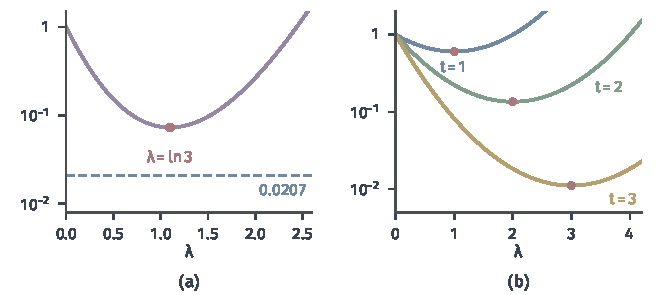
\includegraphics[width=112mm]{figures/07-probability/01-elementary-probability/matplotlib/tail-chernoff-lambda/figure.pdf}
 \caption{指数矩上界作为$\lambda$的函数，纵轴为对数刻度，红点为最小点。(a)$X\sim\operatorname{Bin}(20,1/2)$，$t=15$，紫线为$\mathrm{e}^{-15\lambda}M_X(\lambda)$，最小值$2^{20}/3^{15}\approx0.0731$在$\lambda=\ln3$处取到，蓝色虚线为精确值$0.0207$。(b)$Z\sim\mathcal{N}(0,1)$，$t=1,2,3$时的$\mathrm{e}^{-\lambda t+\lambda^2/2}$，最小点为$\lambda=t$。}
 \label{fig:tail-chernoff-lambda}
\end{BookInlineFigure}

同样的计算适用于一般的二项分布。设$X\sim\operatorname{Bin}(n,p)$，$0<p<1$，阈值写成$na$，$p<a<1$。$M_X(\lambda)=(1-p+p\mathrm{e}^{\lambda})^n$，令导数为零得$\mathrm{e}^{\lambda}=a(1-p)/\bigl(p(1-a)\bigr)$，它大于$1$，所以$\lambda>0$。代回整理，得到
\begin{equation}
 \mathbb{P}(X\geq na)\leq\Bigl[\Bigl(\frac{p}{a}\Bigr)^{a}\Bigl(\frac{1-p}{1-a}\Bigr)^{1-a}\Bigr]^{n} .
 \label{eq:tail-binomial-chernoff-general}
\end{equation}
方括号里的数小于$1$。比例$a$固定时，界随试验次数$n$按几何级数缩小。取$n=20$，$p=1/2$，$a=3/4$，方括号里是$(2/3)^{3/4}2^{1/4}\approx0.8774$，其$20$次方回到$0.0731$。

\paragraph{指数分布}
对$X\sim\operatorname{Exp}(1)$，矩母函数是
\[
 M_X(\lambda)=\int_0^{\infty}\mathrm{e}^{\lambda x}\mathrm{e}^{-x}\,\mathrm{d}x=\begin{cases}\dfrac{1}{1-\lambda}, & \lambda<1,\\ +\infty, & \lambda\geq1 .\end{cases}
\]
$\lambda\geq1$时被积函数不趋于零，积分发散。所以下确界只能在$0<\lambda<1$中取。

对$t>1$，取对数后要最小化的是
\[
 \ln\frac{\mathrm{e}^{-\lambda t}}{1-\lambda}=-\lambda t-\ln(1-\lambda),\qquad 0<\lambda<1 .
\]
它的导数为$-t+1/(1-\lambda)$，零点是$\lambda=1-1/t\in(0,1)$，导数在它左边为负、右边为正。代回得
\begin{equation}
 \mathbb{P}(X\geq t)\leq t\,\mathrm{e}^{1-t},\qquad t>1 .
 \label{eq:tail-exp-chernoff}
\end{equation}
$t\leq1$时导数在$(0,1)$上处处非负，下确界在$\lambda\to0$时取到，界为$1$。

精确值是$\mathrm{e}^{-t}$，两者之比为$\mathrm{e}\,t$：$t=5$时界为$0.0916$，精确值为$0.0067$。指数衰减率$\mathrm{e}^{-t}$被保留了，丢掉的是一个线性因子。原因是$\lambda$不能取到$1$：要完全抓住$\mathrm{e}^{-t}$，需要$\lambda=1$，而那里矩母函数已经是无穷。图~\ref{fig:tail-chernoff-compare}把两个模型上的指数矩上界与较弱的界放在一起。

\begin{BookInlineFigure}
 \centering
 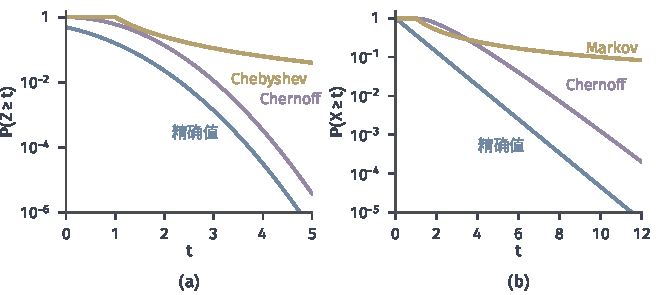
\includegraphics[width=112mm]{figures/07-probability/01-elementary-probability/matplotlib/tail-chernoff-compare/figure.pdf}
 \caption{精确右尾（蓝线）、指数矩上界（紫线）与矩上界（黄线），纵轴为对数刻度。(a)$Z\sim\mathcal{N}(0,1)$：$Q(t)$，$\mathrm{e}^{-t^2/2}$，Chebyshev界$\min\{1,1/t^2\}$。(b)$X\sim\operatorname{Exp}(1)$：$\mathrm{e}^{-t}$，$\min\{1,t\,\mathrm{e}^{1-t}\}$，Markov界$\min\{1,1/t\}$。}
 \label{fig:tail-chernoff-compare}
\end{BookInlineFigure}

\paragraph{指数矩有限与尾部指数衰减}
指数分布的例子说明，矩母函数在哪里有限，与尾部衰减得多快直接相关。图~\ref{fig:tail-mgf-domain}画出三个矩母函数：高斯分布的$\mathrm{e}^{\lambda^2/2}$处处有限；$\operatorname{Exp}(1)$的$1/(1-\lambda)$在$\lambda\to1$时趋于无穷；尺度为$1$的Laplace分布，按同样的积分得$1/(1-\lambda^2)$，只在$\lvert\lambda\rvert<1$时有限。

\begin{BookInlineFigure}
 \centering
 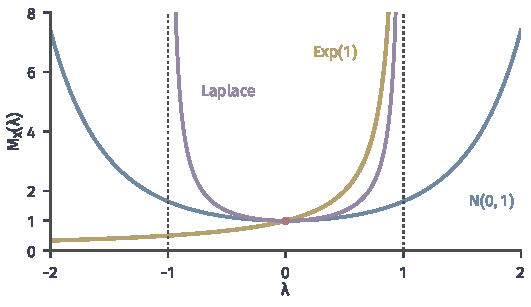
\includegraphics[width=90mm]{figures/07-probability/01-elementary-probability/matplotlib/tail-mgf-domain/figure.pdf}
 \caption{三个矩母函数。蓝线为$\mathcal{N}(0,1)$的$\mathrm{e}^{\lambda^2/2}$，黄线为$\operatorname{Exp}(1)$的$1/(1-\lambda)$（$\lambda<1$），紫线为尺度$1$的Laplace分布的$1/(1-\lambda^2)$（$\lvert\lambda\rvert<1$）。点线标出$\lambda=\pm1$，红点为所有矩母函数共有的$M_X(0)=1$。}
 \label{fig:tail-mgf-domain}
\end{BookInlineFigure}

一个方向已经由式~\eqref{eq:tail-chernoff-lambda}给出：只要某个$\lambda_0>0$使$M_X(\lambda_0)<\infty$，右尾就至少按$\mathrm{e}^{-\lambda_0t}$衰减。对非负、有密度的变量，反方向也成立。

\begin{theorem}[指数矩与尾部衰减]
\label{thm:tail-mgf-decay}
设$X\geq0$有密度，存在常数$C>0$、$c>0$，使$\mathbb{P}(X>s)\leq C\mathrm{e}^{-cs}$对一切$s\geq0$成立。则对$0\leq\lambda<c$，
\begin{equation}
 M_X(\lambda)\leq1+\frac{C\lambda}{c-\lambda}<\infty .
 \label{eq:tail-mgf-decay}
\end{equation}
\end{theorem}

\begin{proof}
在引理~\ref{lem:tail-integral}中取$g(s)=\mathrm{e}^{\lambda s}$，它连续可微且不减，$g(0)=1$，$g'(s)=\lambda\mathrm{e}^{\lambda s}$。于是
\[
 M_X(\lambda)=1+\int_0^{\infty}\lambda\mathrm{e}^{\lambda s}\,\mathbb{P}(X>s)\,\mathrm{d}s .
\]
代入尾部的假设，积分不超过
\[
 \int_0^{\infty}\lambda\mathrm{e}^{\lambda s}\,C\mathrm{e}^{-cs}\,\mathrm{d}s=C\lambda\int_0^{\infty}\mathrm{e}^{-(c-\lambda)s}\,\mathrm{d}s=\frac{C\lambda}{c-\lambda} .
\]
最后一步用到$c-\lambda>0$。
\end{proof}

对$\operatorname{Exp}(1)$，$C=c=1$，式~\eqref{eq:tail-mgf-decay}给出$1+\lambda/(1-\lambda)=1/(1-\lambda)$，与直接计算的结果相同。

\paragraph{重尾时没有指数矩}
尾部只按幂次衰减时，矩母函数在$\lambda>0$处全是无穷。对$\alpha=3$的Pareto分布，由幂级数的一项，$x\geq0$时$\mathrm{e}^{\lambda x}\geq(\lambda x)^3/6$，所以
\[
 M_X(\lambda)\geq\frac{\lambda^3}{6}\,\mathbb{E}[X^3]=+\infty,\qquad \lambda>0 .
\]
三阶矩已经无穷，指数矩更不可能有限。自由度有限的t分布、Cauchy分布也是如此。对这类分布，式~\eqref{eq:tail-chernoff}的下确界里没有任何可用的$\lambda$，只能退回到存在的那些矩。尾部按幂次衰减的分布通常称为\term{重尾分布}（heavy-tailed distribution），它们的矩上界在下一节单独检查。

\paragraph{左尾与双侧}
对左尾，把定理用于$-X$。对$\lambda>0$，事件$\{X\leq t\}$就是$\{-X\geq-t\}$，而$-X$在$\lambda$处的矩母函数是$M_X(-\lambda)$，于是
\begin{equation}
 \mathbb{P}(X\leq t)\leq\inf_{\lambda>0}\mathrm{e}^{\lambda t}M_X(-\lambda) .
 \label{eq:tail-chernoff-left}
\end{equation}
双侧事件按式~\eqref{eq:tail-two-sided}拆成两侧，各用一个界后相加。标准高斯分布关于$0$对称，两侧的界相同，得
\[
 \mathbb{P}(\lvert Z\rvert\geq t)\leq2\mathrm{e}^{-t^2/2},\qquad t>0 .
\]

\paragraph{本节的边界}
这里只用了单个随机变量的矩母函数。矩母函数还有两方面的用途：在一定条件下它决定分布本身，这类识别工具在第~\ref{chap:weak-convergence-of-distributions}章介绍；对许多独立量之和，它可以分解成各项矩母函数的乘积，于是式~\eqref{eq:tail-chernoff}给出样本平均偏离均值的指数界，可参考\BookChapterRef{chap:finite-sample-error-bounds}{卷八第4章“有限样本的误差上界”}。


\section{上界的评价}
\label{sec:tail-bound-comparison}

前面几节各自给出了一个界，每次都和精确值比了一比。现在把它们放在同一个变量、同一个阈值上，回答三个问题：每个界用了多少信息，在什么阈值上才有用，信息不全或矩不存在时还剩下什么。

\paragraph{同一事件上的排列}
对贯穿例子的事件$\{X\geq15\}$，表~\ref{tab:tail-bounds}列出各个界及其所需的信息。四阶、六阶矩界以$a=10$为中心，作用于包含$\{X\geq15\}$的双侧事件$\{\lvert X-10\rvert\geq5\}$；表的最后一行留到后面解释。

\begin{BookInlineTable}
 \centering
 \caption{$X\sim\operatorname{Bin}(20,1/2)$时$\mathbb{P}(X\geq15)$的精确值与各个上界。比值为上界除以精确值$0.0207$。}
 \label{tab:tail-bounds}
 \begin{tabular}{lllr}
  \toprule
  方法 & 所用信息 & 数值 & 比值\\
  \midrule
  精确值 & 完整质量表 & $0.0207$ & $1$\\
  Markov & $X\geq0$，$\mathbb{E}[X]=10$ & $0.667$ & $32$\\
  Chebyshev & $\mathbb{E}[X]$，$\operatorname{Var}(X)=5$ & $0.200$ & $9.7$\\
  四阶矩 & $m_4=72.5$ & $0.116$ & $5.6$\\
  六阶矩 & $m_6=1692.5$ & $0.108$ & $5.2$\\
  指数矩 & $M_X(\lambda)$，$\lambda>0$ & $0.0731$ & $3.5$\\
  最优原点矩 & $\mathbb{E}[X^k]$，$k\leq60$ & $0.0646$ & $3.1$\\
  \bottomrule
 \end{tabular}
\end{BookInlineTable}

图~\ref{fig:tail-bounds-bar}在对数刻度上画出同样的数。越往下，用到的信息越多，界越小，但即使是最好的界也比精确值大三倍。差距不会消失，因为每个界都是对一整类分布的保证：只要另一个分布与$X$有相同的已知数值而尾部更重，界就必须照顾它。

\begin{BookInlineFigure}
 \centering
 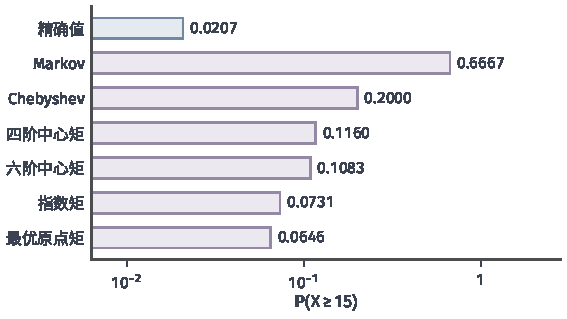
\includegraphics[width=96mm]{figures/07-probability/01-elementary-probability/matplotlib/tail-bounds-bar/figure.pdf}
 \caption{$X\sim\operatorname{Bin}(20,1/2)$时$\mathbb{P}(X\geq15)$的精确值（蓝）与各个上界（紫），横轴为对数刻度，数字为数值。四阶、六阶中心矩以$10$为中心；最优原点矩在$k=1,\dots,60$中取$\mathbb{E}[X^k]/15^k$的最小值，于$k=17$取到。}
 \label{fig:tail-bounds-bar}
\end{BookInlineFigure}

\paragraph{矩与指数矩的关系}
表中最后一行用的是原点矩$\mathbb{E}[X^k]$，对每个$k$由质量表求和，然后取$\mathbb{E}[X^k]/15^k$的最小值，在$k=17$处得到$0.0646$，竟比指数矩上界还小。这不是巧合：对非负变量，最好的矩上界从来不劣于指数矩上界。

\begin{theorem}[最优矩上界不劣于指数矩上界]
\label{thm:tail-moment-vs-chernoff}
设$Y\geq0$，$t>0$，$\lambda>0$且$M_Y(\lambda)<\infty$。则
\begin{equation}
 \inf_{k=0,1,2,\dots}\frac{\mathbb{E}[Y^k]}{t^k}\leq\mathrm{e}^{-\lambda t}M_Y(\lambda) .
 \label{eq:tail-moment-vs-chernoff}
\end{equation}
\end{theorem}

\begin{proof}
把$\mathrm{e}^{\lambda Y}$展成幂级数，各项$\lambda^kY^k/k!$都非负。非负项的级数可以与求和或积分交换次序，依据与引理~\ref{lem:tail-integral}证明中交换积分次序的依据相同，所以
\[
 M_Y(\lambda)=\sum_{k\geq0}\frac{\lambda^k\,\mathbb{E}[Y^k]}{k!} .
\]
两边乘$\mathrm{e}^{-\lambda t}$，并把每项写成“权重乘矩上界”：
\[
 \mathrm{e}^{-\lambda t}M_Y(\lambda)=\sum_{k\geq0}\Bigl(\mathrm{e}^{-\lambda t}\frac{(\lambda t)^k}{k!}\Bigr)\cdot\frac{\mathbb{E}[Y^k]}{t^k} .
\]
括号里的权重是参数为$\lambda t$的Poisson分布的质量，非负且和为$1$。记$b=\inf_k\mathbb{E}[Y^k]/t^k$，每个矩上界都不小于$b$，所以加权和不小于$b$：
\[
 \mathrm{e}^{-\lambda t}M_Y(\lambda)\geq b\sum_{k\geq0}\mathrm{e}^{-\lambda t}\frac{(\lambda t)^k}{k!}=b .
\]
这就是式~\eqref{eq:tail-moment-vs-chernoff}。
\end{proof}

证明说明了两者的关系：指数矩上界是各阶矩上界按Poisson权重的平均，平均值不会小于其中最小的一项。对右边取下确界后结论仍成立，所以式~\eqref{eq:tail-chernoff}的Chernoff界总不小于最优矩上界。定理要求$Y$非负，并且比较的是关于$0$的原点矩；对一般的$X$和单侧事件，可以取$Y=X$（当$X\geq0$时）或$Y=\lvert X-a\rvert$。

图~\ref{fig:tail-moment-vs-chernoff}在$Y=\lvert Z\rvert$、$Z\sim\mathcal{N}(0,1)$上验证这一点。$\lvert Z\rvert$的矩母函数为$2\mathrm{e}^{\lambda^2/2}\Phi(\lambda)$，其中$\Phi$是标准高斯分布函数，下确界需要数值计算。在$t=3$处，精确值、最优矩上界和指数矩上界依次为
\[
 0.0027,\qquad 0.0156,\qquad 0.0222 .
\]
两个界的差距不大，量级相同。

\begin{BookInlineFigure}
 \centering
 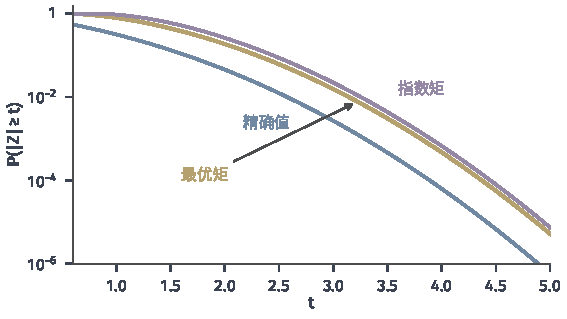
\includegraphics[width=96mm]{figures/07-probability/01-elementary-probability/matplotlib/tail-moment-vs-chernoff/figure.pdf}
 \caption{$Z\sim\mathcal{N}(0,1)$的$\mathbb{P}(\lvert Z\rvert\geq t)$（蓝线）、对实数阶$p>0$取最小的矩上界$\inf_p\mathbb{E}\lvert Z\rvert^p/t^p$（黄线）与$\lvert Z\rvert$的指数矩上界$\inf_{\lambda>0}\mathrm{e}^{-\lambda t}M_{\lvert Z\rvert}(\lambda)$（紫线），纵轴为对数刻度。}
 \label{fig:tail-moment-vs-chernoff}
\end{BookInlineFigure}

既然矩上界更紧，为什么还要指数矩？原因在计算。最优矩上界要求知道全部各阶矩，再对阶数搜索；指数矩把它们压缩成一个函数，常常有闭式，例如二项分布的$\bigl((1+\mathrm{e}^{\lambda})/2\bigr)^{20}$，只需一维最小化。对独立量之和，矩母函数还能分解成乘积，而高阶矩的展开会迅速变得繁琐。

\paragraph{反过来求试验次数}
界的差距在反问题中看得更清楚。掷$n$次均匀硬币，正面次数$X\sim\operatorname{Bin}(n,1/2)$，正面比例是$X/n$。要使比例偏离$1/2$至少$0.1$的概率不超过$0.05$，$n$至少要多大？

先用Chebyshev不等式。由第~\ref{chap:common-distributions}章，$\operatorname{Var}(X)=n/4$；由缩放规律，$\operatorname{Var}(X/n)=1/(4n)$。于是
\[
 \mathbb{P}\Bigl(\Bigl\lvert\frac{X}{n}-\frac12\Bigr\rvert\geq0.1\Bigr)\leq\frac{1/(4n)}{0.01}=\frac{25}{n} .
\]
要使右边不超过$0.05$，需要$n\geq500$。

再用指数矩上界。右侧事件是$\{X\geq0.6n\}$，在式~\eqref{eq:tail-binomial-chernoff-general}中取$p=1/2$，$a=0.6$，方括号里的数是
\[
 \Bigl(\frac{0.5}{0.6}\Bigr)^{0.6}\Bigl(\frac{0.5}{0.4}\Bigr)^{0.4}=\mathrm{e}^{-0.02014}\approx0.9801 .
\]
由对称性左侧事件$\{X\leq0.4n\}$有同样的界，两侧相加得$2\mathrm{e}^{-0.02014n}$。令它不超过$0.05$，解得$n\geq\ln40/0.02014\approx183.2$，即$n\geq184$。

最后用质量表直接计算。精确概率随$n$的变化并不单调，因为$0.6n$是否为整数会影响端点上的质量：$n=97$时约为$0.0417$，$n=100$时又升到$0.0569$。逐个计算可知，从$n=106$起精确概率都不超过$0.05$（数值检查到$n=500$）。三种方法给出的次数是$500$、$184$与$106$。上界越紧，为同一个保证付出的试验次数越少；精确计算最省，但要对每个$n$求和，而且只适用于确知的分布。

\paragraph{有效阈值}
每个界只在一段阈值上提供信息，在其余阈值上不小于$1$。Markov界在$t\leq\mathbb{E}[X]$时不小于$1$；Chebyshev界在$t\leq\sigma$时不小于$1$。指数矩上界在$t\leq\mathbb{E}[X]$时也给不出信息：由第~\ref{chap:random-variable-moments}章的Jensen不等式，$\mathrm{e}^{\lambda x}$是凸函数，所以
\[
 \mathrm{e}^{-\lambda t}M_X(\lambda)\geq\mathrm{e}^{-\lambda t}\mathrm{e}^{\lambda\mathbb{E}[X]}=\mathrm{e}^{\lambda(\mathbb{E}[X]-t)}\geq1,\qquad \lambda>0 .
\]
这符合直觉：阈值不在均值右边时，“越过阈值”并不是一个罕见事件。实际使用时把每个界与$1$取较小者，例如写成$\min\{1,\mathbb{E}[X]/t\}$；图中所有的界都已这样截断。

\paragraph{重尾模型}
对$\alpha=3$的Pareto分布，指数矩不存在，三阶及以上的矩也不存在，能用的只有$p<3$阶的矩。由$\mathbb{E}[X^p]=3/(3-p)$，原点矩上界是
\[
 \mathbb{P}(X\geq t)\leq\frac{3}{(3-p)\,t^{p}},\qquad 0<p<3 .
\]
$p$越接近$3$，$t^{-p}$衰减越快，但系数$3/(3-p)$越大。对给定的$t$，把对数$\ln3-\ln(3-p)-p\ln t$对$p$求导并令其为零：
\[
 \frac{1}{3-p}-\ln t=0,\qquad p^{*}=3-\frac{1}{\ln t} .
\]
当$t>\mathrm{e}^{1/3}\approx1.40$时$p^{*}\in(0,3)$，二阶导数$1/(3-p)^2>0$，这是最小点。

代回去，$3-p^{*}=1/\ln t$，$t^{-p^{*}}=t^{-3}\,t^{1/\ln t}=\mathrm{e}\,t^{-3}$，于是
\begin{equation}
 \inf_{0<p<3}\frac{3}{(3-p)\,t^{p}}=\frac{3\mathrm{e}\ln t}{t^{3}},\qquad t>\mathrm{e}^{1/3} .
 \label{eq:tail-pareto-best}
\end{equation}
精确值是$t^{-3}$，最好的原点矩上界多出一个因子$3\mathrm{e}\ln t$，随$t$缓慢增大。$t=10$时，界为$0.0188$，精确值为$0.001$。图~\ref{fig:tail-pareto-moments}在双对数坐标中画出这些曲线：每个固定阶数的界是一条斜率为$-p$的直线，红色虚线是它们的下包络。

\begin{BookInlineFigure}
 \centering
 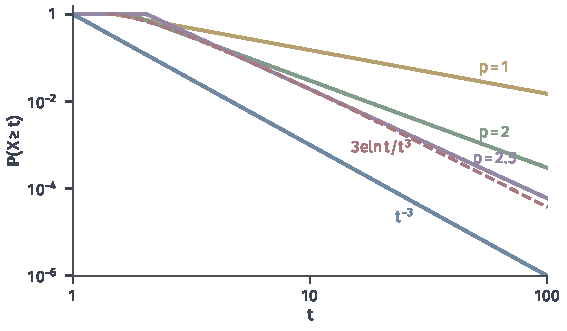
\includegraphics[width=96mm]{figures/07-probability/01-elementary-probability/matplotlib/tail-pareto-moments/figure.pdf}
 \caption{$\alpha=3$的Pareto分布，双对数坐标。蓝线为精确尾部$t^{-3}$，黄、绿、紫线为$p=1,2,2.5$的原点矩上界$\min\{1,3/((3-p)t^p)\}$，红色虚线为对$p\in(0,3)$取最小的包络$3\mathrm{e}\ln t/t^3$。}
 \label{fig:tail-pareto-moments}
\end{BookInlineFigure}

中心的选择同样重要。Pareto分布的均值为$3/2$，方差为$3-9/4=3/4$。对$t>3/2$，事件$\{X\geq t\}$包含在$\{\lvert X-3/2\rvert\geq t-3/2\}$中，Chebyshev不等式给出$\tfrac34/(t-\tfrac32)^2$。$t=10$时这是$0.0104$，反而比式~\eqref{eq:tail-pareto-best}的$0.0188$更好；$t=100$时它是$7.7\times10^{-5}$，又不如后者的$3.8\times10^{-5}$。以均值为中心去掉了原点处的偏移，在中等阈值上更有利；阈值很远时，阶数的作用占了上风。

更重的尾部会让可用的工具进一步减少。Cauchy分布连均值都没有，Markov不等式和Chebyshev不等式都不能用，只剩阶数$p<1$的绝对矩上界。这时尾概率本身也只按$1/t$衰减，任何依赖高阶矩的估计都无从谈起。

\paragraph{信息与代价}
图~\ref{fig:tail-information-ladder}把本章的界按所需信息排列。越往下，假设越强：均值有限弱于方差有限，方差有限弱于更高阶矩有限，而某个$\lambda>0$处指数矩有限蕴含一切阶矩有限。假设越强，界越紧，适用的分布越少。完整分布在最下面，它给出精确值，但需要的信息最多，计算也可能最难，例如高斯尾部$Q(t)$就要数值积分。

\begin{BookInlineFigure}
 \centering
 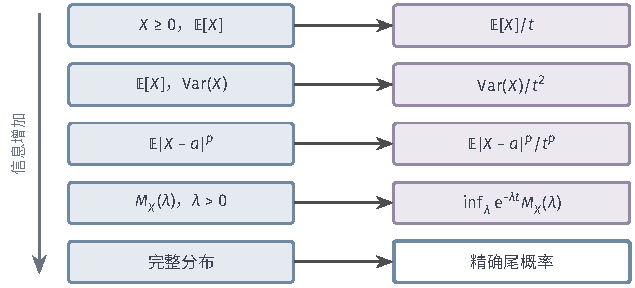
\includegraphics[width=108mm]{figures/07-probability/01-elementary-probability/tikz/tail-information-ladder/figure.pdf}
 \caption{所用信息（左）与得到的尾部结论（右）。前两行分别控制$\mathbb{P}(X\geq t)$与$\mathbb{P}(\lvert X-\mathbb{E}[X]\rvert\geq t)$，第三行控制$\mathbb{P}(\lvert X-a\rvert\geq t)$，第四行控制$\mathbb{P}(X\geq t)$。自上而下大致按所需的矩条件由弱到强排列，紫色为上界，白色为精确值。}
 \label{fig:tail-information-ladder}
\end{BookInlineFigure}

计算成本按相反方向排列。Markov界和Chebyshev界只要一两个数，一次除法；矩上界要计算一个积分或求和；指数矩上界要先得到矩母函数，再做一维最小化，可以求导，也可以数值搜索；精确值要对整个尾部求和或积分。实际选择时先问手上有什么信息，再问需要多紧的保证。

\paragraph{保证与估计}
最后要分清三种数。精确尾概率是具体分布的性质。Markov界和Chebyshev界在各自的信息下是最好的保证，第~\ref{sec:tail-markov}节和第~\ref{sec:tail-chebyshev}节的极端分布达到了它们，所以不能指望仅凭这些信息改进。矩上界与指数矩上界则依赖额外的假设：高阶矩或指数矩存在，并且已知其数值。额外的假设换来了更紧的界，也缩小了适用范围；假设一旦不成立，例如遇到重尾模型，就要退回到弱的界。


\section{本章小结}
\label{sec:tail-summary}

本章从尾事件出发。右尾$\{X\geq t\}$、左尾$\{X\leq t\}$与双侧事件$\{\lvert X-a\rvert\geq t\}$的概率都可以由分布函数算出，但端点要分清：含原子时$\mathbb{P}(X\geq t)=1-F_X(t^-)$，比$1-F_X(t)$多出$\mathbb{P}(X=t)$；双侧事件拆成两个不相交的单侧事件，不对称的分布要两侧分别计算。对非负变量，期望是生存函数下的面积，各阶矩也由尾部决定，尾部衰减得慢，高阶矩就不存在。

只知道少量数值特征时，所有的界都来自同一个想法：用一个非负不减的函数从上方压住尾事件的示性函数，再取期望。压法不同，用到的信息就不同。非负变量的均值给出Markov不等式$\mathbb{E}[X]/t$；方差给出Chebyshev不等式$\sigma^2/t^2$；$p$阶绝对矩给出按$t^{-p}$衰减的界；指数矩给出Chernoff界$\inf_{\lambda>0}\mathrm{e}^{-\lambda t}M_X(\lambda)$，在高斯和二项模型上它能抓住尾部的指数衰减。

这些界要与真实概率分开理解。Markov界和Chebyshev界在各自的信息下不能改进，两点和三点极端分布达到它们，所以与具体模型的差距来自信息不足，而不是论证粗糙。更高阶的矩和指数矩是额外的假设：它们给出更紧的界，但要求更强的存在条件，阶数越高也不保证对每个阈值越好。对非负变量，最优的矩上界不劣于指数矩上界，指数矩的优势在于便于计算。重尾模型把这些限制暴露出来：Pareto分布只有低阶矩，Cauchy分布连均值都没有，可用的界随之变弱；界大于$1$时直接与平凡界$1$取较小者。

后面的章节会反复回到这些不等式。判断一列随机变量是否越来越集中在某个值附近，说明许多次独立试验的平均值稳定在均值附近，以及保证用随机样本估计积分时误差不太大，出发点都是Markov和Chebyshev不等式；把指数矩用于许多独立量之和，则得到随试验次数指数缩小的误差保证。


\chapter{随机向量}
\label{chap:random-vectors}

同一个房间里装了两台温度传感器，每台把读数粗分成三档：$0$表示偏低，$1$表示正常，$2$表示偏高。前几章的工具可以分别描述每台传感器：它读“偏高”的概率是多少，读数的平均档位和波动有多大，读数超过某个档位的概率有多小。可是值班人员真正关心的问题常常同时涉及两台：两台同时报“偏高”的机会有多大？第一台读“偏低”时，第二台还可能读“偏高”吗？把两台读数取平均，波动能比一台小多少？

这些问题都在问两个量在同一次观测中怎样共同取值。只知道每台传感器各自的分布，回答不了它们；需要一份记录“哪一对读数以多大概率一起出现”的规律。本章把同时观察的几个随机变量合成一个随机向量，研究这份共同规律包含什么信息，又怎样从中取出常用的部分。

本章分四步展开。第一节建立联合分布，用概率表、联合密度和联合分布函数描述它，并说明怎样取出单个分量的边缘分布，以及为什么反过来不行。第二节讨论联合分布恰好由边缘决定的情形，即独立。第三节用均值向量和协方差矩阵概括联合分布的中心与波动，解释交叉项从哪里来。第四节固定一个变量的取值，重新归一化，得到条件分布、条件均值和全方差公式。

全章以两台传感器的概率表和三角形上的均匀密度为贯穿例子，前者代表离散情形，后者代表连续情形。具体的多元分布模型在第~\ref{chap:multivariate-distributions}章介绍，随机向量经过变换以后的分布在第~\ref{chap:random-variable-transformations}章计算。

\section{联合分布}
\label{sec:rvc-joint}

两台传感器各自的读数规律，第~\ref{chap:random-variables}章已经会写：每台都有一张概率表。要回答“两台同时报偏高”这样的问题，需要的却是读数\emph{对}的概率。这一节先说明几个随机变量怎样放进同一次试验，再用概率表、密度和分布函数记录它们的共同规律，最后从共同规律中取出单个分量的规律。

\paragraph{同一次试验中的几个随机变量}
随机变量是样本空间$\Omega$上的函数：试验给出一个样本点$\omega$，随机变量把它变成一个数。几个随机变量要能“一起取值”，必须定义在同一个$\Omega$上，这样同一个$\omega$同时决定它们全部的值。

掷两颗均匀骰子是最直接的例子。样本空间由$36$个等可能的有序对$(i,j)$组成，$i$是第一颗的点数，$j$是第二颗的点数。令$X$为第一颗的点数，$M$为两颗中较大的点数，即
\[
 X(i,j)=i,\qquad M(i,j)=\max\{i,j\}.
\]
每个样本点同时给出一对值$(X,M)$。事件$\{X=4,\,M=4\}$由第一颗为$4$、第二颗不超过$4$的四个样本点组成，概率是$4/36$；事件$\{X=2,\,M=5\}$只含样本点$(2,5)$，概率是$1/36$。

把$36$个样本点按它们给出的$(X,M)$分组，每组的点数除以$36$，就得到每一对取值的概率，见图~\ref{fig:rvc-dice-map}。表中右下方的空格表示$M<X$的取值对，它们不可能出现，因为较大点数不会小于第一颗的点数。这张表记录的正是“两个量怎样一起取值”。

\begin{BookInlineFigure}
  \centering
  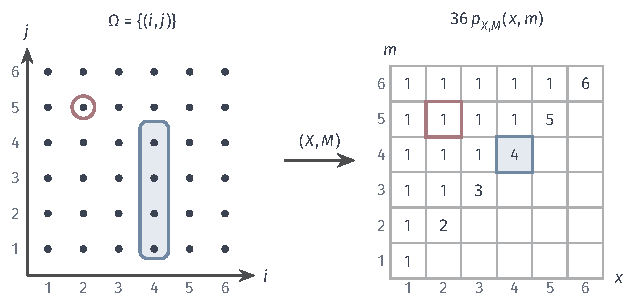
\includegraphics[width=107mm]{figures/07-probability/01-elementary-probability/tikz/rvc-dice-map/figure.pdf}
  \caption{从样本点到联合概率表。左侧是两颗骰子的$36$个样本点，横坐标为第一颗点数$i$，纵坐标为第二颗点数$j$。右侧格子$(x,m)$中的数是满足$X=x$、$M=m$的样本点个数，除以$36$即为概率。蓝框中的四个样本点都给出$(X,M)=(4,4)$，红圈中的样本点$(2,5)$单独给出$(2,5)$；空格的概率为零。}
  \label{fig:rvc-dice-map}
\end{BookInlineFigure}

\begin{definition}[随机向量与联合分布]
\label{def:rvc-random-vector}
设$X_1,\dots,X_d$是定义在同一样本空间$\Omega$上的随机变量。把它们排成列向量
\begin{equation}
 \bm{X}=(X_1,\dots,X_d)^{\top},
 \label{eq:rvc-random-vector}
\end{equation}
称为$d$维\term{随机向量}（random vector）。对$\mathbb{R}^{d}$中的集合$A$，事件$\{\bm{X}\in A\}$由使$\bm{X}(\omega)\in A$的样本点组成；这些事件的概率$\mathbb{P}(\bm{X}\in A)$合起来称为$\bm{X}$的\term{联合分布}（joint distribution）。
\end{definition}

本部分只处理能用求和或普通积分算出概率的集合$A$，例如有限点集、矩形和卷二能够积分的平面区域；对哪些集合赋予概率的一般规定在第~\ref{chap:probability-spaces}章给出。随机向量与它的联合分布是两件事，这一点和一元情形相同。$\bm{X}$是$\Omega$上的函数，回答“这次试验得到哪个向量”；联合分布只回答“各个区域的向量出现的概率是多少”。两颗骰子的$(X,M)$和后面许多问题只需要联合分布，但只有回到$\Omega$，才能说清几个量为什么会一起变化。

\paragraph{联合概率表}
两个变量都只取有限个或可数个值时，每一对取值的概率就足以计算一切。仍用大写字母表示随机变量、小写字母表示取值，定义
\begin{equation}
 p_{X,Y}(x,y)=\mathbb{P}(X=x,\,Y=y),
 \label{eq:rvc-joint-pmf}
\end{equation}
称为$(X,Y)$的\term{联合质量函数}（joint probability mass function）。它非负，对全部取值对求和等于$1$。

事件$\{(X,Y)\in A\}$可以按取值对拆成互斥的单点事件，由可加性，
\begin{equation}
 \mathbb{P}\bigl((X,Y)\in A\bigr)=\sum_{(x,y)\in A}p_{X,Y}(x,y).
 \label{eq:rvc-joint-pmf-event}
\end{equation}
把概率想象成总量为$1$的质量，联合质量函数就是把这份质量分配到平面上的一些格点；任何联合事件的概率，等于事件圈住的格点上的质量之和。

回到两台传感器。设第一台的档位为$X$，第二台为$Y$，作为教学示例，取图~\ref{fig:rvc-sensor-table}中的概率表。九个数之和为$1$。两台不会一台读$0$、另一台读$2$，相邻档位的组合各占$0.10$，对角线上的组合各占$0.20$：两台读数倾向于一致，但并不总是一致。

\begin{BookInlineFigure}
  \centering
  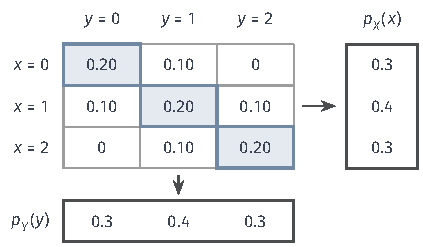
\includegraphics[width=72mm]{figures/07-probability/01-elementary-probability/tikz/rvc-sensor-table/figure.pdf}
  \caption{两台传感器档位的联合概率表。行对应第一台的档位$x$，列对应第二台的档位$y$。浅蓝格子组成事件$\{X=Y\}$；右侧方框是各行之和$p_X(x)$，下方方框是各列之和$p_Y(y)$。}
  \label{fig:rvc-sensor-table}
\end{BookInlineFigure}

由式~\eqref{eq:rvc-joint-pmf-event}，读数一致的概率是对角线三格之和，读数之和至少为$3$的概率是右下角三格之和：
\[
 \mathbb{P}(X=Y)=0.20+0.20+0.20=0.60,
\]
\[
 \mathbb{P}(X+Y\geq 3)=p_{X,Y}(1,2)+p_{X,Y}(2,1)+p_{X,Y}(2,2)=0.40.
\]
两台同时报偏高的概率就是一个格子：$\mathbb{P}(X=2,\,Y=2)=0.20$。这些问题都无法只用每台各自的概率表回答。

\paragraph{联合密度}
如果两个量连续取值，单个点的概率为零，概率表不再适用。一元情形用密度表示单位长度上的质量；平面上相应地用单位面积上的质量。

\begin{definition}[联合密度]
\label{def:rvc-joint-density}
设$f_{X,Y}$是平面上的非负函数。若对每个矩形$R=[a_1,b_1]\times[a_2,b_2]$都有
\begin{equation}
 \mathbb{P}\bigl((X,Y)\in R\bigr)=\iint_{R}f_{X,Y}(x,y)\,\mathrm{d}x\,\mathrm{d}y,
 \label{eq:rvc-joint-density}
\end{equation}
则称$f_{X,Y}$为$(X,Y)$的\term{联合密度}（joint density）。
\end{definition}

矩形概率确定以后，整个联合分布也就确定了：对卷二能够积分的区域$A$，$\mathbb{P}((X,Y)\in A)$同样等于$f_{X,Y}$在$A$上的积分。这一事实的证明需要第~\ref{chap:probability-spaces}章的工具，这里直接使用。多重积分、累次积分以及无界区域上非负函数积分的计算规则，可参考\BookChapterRef{chap:region-integrals}{卷二第24章“区域积分”}。取$A$为整个平面，可知联合密度的积分等于$1$。

联合密度本身不是概率。在点$(x,y)$附近取边长为$h$和$k$的小矩形，若$f_{X,Y}$在该点附近连续，矩形的概率约为$f_{X,Y}(x,y)\,hk$；密度大的地方，同样面积上的概率多。$d$维情形把二重积分换成$d$重积分，把面积换成体积即可。

现在建立贯穿全章的连续例子。令点$(X,Y)$在三角形$T=\{(x,y):0\leq y\leq x\leq 1\}$上均匀分布，即
\begin{equation}
 f_{X,Y}(x,y)=\begin{cases}2,&0\leq y\leq x\leq 1,\\0,&\text{其他}.\end{cases}
 \label{eq:rvc-triangle-density}
\end{equation}
三角形的面积是$1/2$，所以常数取$2$才能使总积分为$1$。“均匀”指同样面积的区域只要都落在三角形内，概率就相同。

求$\mathbb{P}(X+Y\leq 1)$。事件在三角形内对应的部分是顶点为$(0,0)$、$(1,0)$、$(1/2,1/2)$的小三角形，见图~\ref{fig:rvc-triangle-density}(a)。固定$y\in[0,1/2]$，$x$从$y$走到$1-y$，先对$x$积分：
\[
 \mathbb{P}(X+Y\leq 1)=\int_{0}^{1/2}\!\!\int_{y}^{1-y}2\,\mathrm{d}x\,\mathrm{d}y
 =\int_{0}^{1/2}2(1-2y)\,\mathrm{d}y.
\]
再对$y$积分，
\[
 \int_{0}^{1/2}2(1-2y)\,\mathrm{d}y=\Bigl[2y-2y^{2}\Bigr]_{0}^{1/2}=\frac12 .
\]
密度是常数时，概率就是“事件区域面积乘以$2$”：小三角形的面积是$1/4$，结果相同。

\begin{BookInlineFigure}
  \centering
  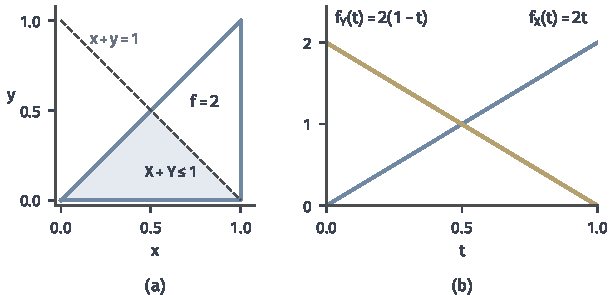
\includegraphics[width=104mm]{figures/07-probability/01-elementary-probability/matplotlib/rvc-triangle-density/figure.pdf}
  \caption{三角形上的均匀密度。(a)蓝线围成的三角形内密度为$2$，其外为$0$；浅蓝区域是事件$\{X+Y\leq 1\}$，概率$1/2$，虚线为$x+y=1$。(b)两个边缘密度：$f_X(t)=2t$（蓝）与$f_Y(t)=2(1-t)$（黄），$t\in[0,1]$。}
  \label{fig:rvc-triangle-density}
\end{BookInlineFigure}

\paragraph{联合分布函数}
概率表只适用于离散情形，联合密度只适用于连续情形。与一元情形一样，分布函数对两类模型都有意义。对$d$维随机向量定义\term{联合分布函数}（joint distribution function）
\begin{equation}
 F_{\bm{X}}(\bm{x})=\mathbb{P}(X_1\leq x_1,\dots,X_d\leq x_d),\qquad \bm{x}\in\mathbb{R}^{d}.
 \label{eq:rvc-joint-cdf}
\end{equation}
二维时，$F_{X,Y}(x,y)$是点$(x,y)$左下方整个象限的概率，见图~\ref{fig:rvc-cdf-rectangle}(a)。

矩形的概率可以由四个角上的分布函数值算出。设$a_1<b_1$，$a_2<b_2$，记$R=(a_1,b_1]\times(a_2,b_2]$。从象限$\{X\leq b_1,Y\leq b_2\}$中去掉$\{X\leq a_1,Y\leq b_2\}$和$\{X\leq b_1,Y\leq a_2\}$，两者的公共部分$\{X\leq a_1,Y\leq a_2\}$被去掉了两次，需要加回一次，于是
\begin{equation}
 \begin{aligned}
 \mathbb{P}\bigl((X,Y)\in R\bigr)
 &=F_{X,Y}(b_1,b_2)-F_{X,Y}(a_1,b_2)\\
 &\quad-F_{X,Y}(b_1,a_2)+F_{X,Y}(a_1,a_2).
 \end{aligned}
 \label{eq:rvc-rectangle}
\end{equation}
图~\ref{fig:rvc-cdf-rectangle}(b)中四个角上的符号就是这四项的正负号。由此可见，分布函数确定全部矩形的概率，从而确定联合分布。

\begin{BookInlineFigure}
  \centering
  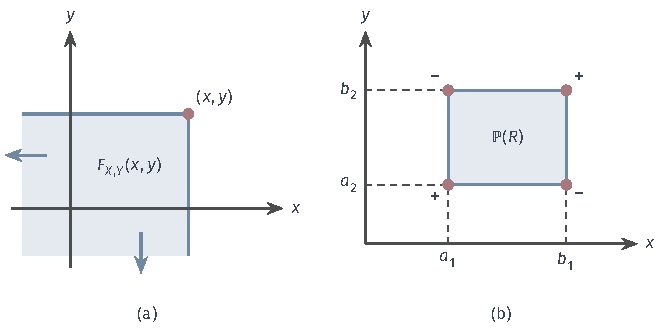
\includegraphics[width=112mm]{figures/07-probability/01-elementary-probability/tikz/rvc-cdf-rectangle/figure.pdf}
  \caption{联合分布函数与矩形概率。(a)$F_{X,Y}(x,y)$是红点左下方象限（浅蓝，向左、向下无界）的概率。(b)矩形$R=(a_1,b_1]\times(a_2,b_2]$的概率等于四个角上分布函数值的带符号和，符号标在各角旁。}
  \label{fig:rvc-cdf-rectangle}
\end{BookInlineFigure}

对三角形模型，$0\leq y\leq x\leq 1$时，左下方象限与三角形的交是梯形$\{(s,t):t\leq s\leq x,\ t\leq y\}$，面积为$xy-y^{2}/2$，乘以密度$2$得
\[
 F_{X,Y}(x,y)=2xy-y^{2},\qquad 0\leq y\leq x\leq 1 .
\]
$0\leq x<y\leq 1$时，象限与三角形的交是$\{t\leq s\leq x\}$，$F_{X,Y}(x,y)=x^{2}$。代入式~\eqref{eq:rvc-rectangle}检验矩形$(1/2,1]\times(0,1/2]$的概率：
\[
 F_{X,Y}(1,\tfrac12)-F_{X,Y}(\tfrac12,\tfrac12)-F_{X,Y}(1,0)+F_{X,Y}(\tfrac12,0)
 =\tfrac34-\tfrac14-0+0=\tfrac12 .
\]
这个正方形整个落在三角形内，面积$1/4$乘以密度$2$也是$1/2$。

\paragraph{边缘分布}
有了联合分布，常常又只关心其中一个分量，例如只问第一台传感器的读数。事件$\{X=x\}$可以按$Y$的取值拆成互斥事件$\{X=x,Y=y\}$的并，由可加性得到
\begin{equation}
 p_X(x)=\sum_{y}p_{X,Y}(x,y),\qquad p_Y(y)=\sum_{x}p_{X,Y}(x,y).
 \label{eq:rvc-marginal-pmf}
\end{equation}
在概率表上，这就是按行求和或按列求和。图~\ref{fig:rvc-sensor-table}中两台传感器的规律相同：
\[
 p_X=p_Y=(0.3,\,0.4,\,0.3).
\]

有联合密度时，取矩形$[a,b]\times[-c,c]$，令$c\to\infty$，先对$y$积分，得到
\[
 \mathbb{P}(a\leq X\leq b)=\int_{a}^{b}\Bigl(\int_{-\infty}^{\infty}f_{X,Y}(x,y)\,\mathrm{d}y\Bigr)\mathrm{d}x .
\]
这里交换顺序与取极限的依据是非负函数的累次积分。上式说明括号里的函数就是$X$的密度：
\begin{equation}
 f_X(x)=\int_{-\infty}^{\infty}f_{X,Y}(x,y)\,\mathrm{d}y,\qquad f_Y(y)=\int_{-\infty}^{\infty}f_{X,Y}(x,y)\,\mathrm{d}x.
 \label{eq:rvc-marginal-density}
\end{equation}
由联合分布得到的单个分量的分布称为\term{边缘分布}（marginal distribution），对其余分量求和或积分的操作称为\term{边缘化}（marginalization）。名称来自概率表：行和与列和写在表的边上。

对三角形模型，固定$x\in[0,1]$，密度只在$0\leq y\leq x$上取$2$；固定$y\in[0,1]$，密度只在$y\leq x\leq 1$上取$2$。于是
\[
 f_X(x)=\int_{0}^{x}2\,\mathrm{d}y=2x,\qquad f_Y(y)=\int_{y}^{1}2\,\mathrm{d}x=2(1-y),
\]
两式都在$[0,1]$上成立，见图~\ref{fig:rvc-triangle-density}(b)。$X$的质量偏向$1$，$Y$的质量偏向$0$：三角形在右侧竖得高，在下方铺得宽。

两颗骰子的例子也可以这样核对。图~\ref{fig:rvc-dice-map}右表中第$m$行有$m-1$个$1$和一个$m$，按行求和得到较大点数的边缘分布
\[
 p_M(m)=\frac{(m-1)+m}{36}=\frac{2m-1}{36},\qquad m=1,\dots,6 .
\]
六个值依次为$1/36,3/36,\dots,11/36$，和为$1$；较大点数偏向大的值。直接从样本空间看，$\{M\leq m\}$要求两颗都不超过$m$，概率为$m^{2}/36$，相邻两项相减同样得到$(2m-1)/36$。

$d$维时规则相同：保留哪些分量，就对其余全部分量求和或积分。例如三维密度$f(x_1,x_2,x_3)$对$x_3$积分得到$(X_1,X_2)$的二维边缘密度，再对$x_2$积分得到$X_1$的边缘密度。用分布函数表示，边缘分布函数是把其余坐标推向$+\infty$的极限，例如$F_X(x)=\lim_{y\to\infty}F_{X,Y}(x,y)$。

\paragraph{相同的边缘，不同的联合}
边缘化把其他分量的信息汇总掉了，这一步一般不能逆转。图~\ref{fig:rvc-same-marginals}把传感器表与另一张表并排放置：右表的每个格子取行和与列和的乘积。两张表的行和、列和完全一样，联合规律却不同。

\begin{BookInlineFigure}
  \centering
  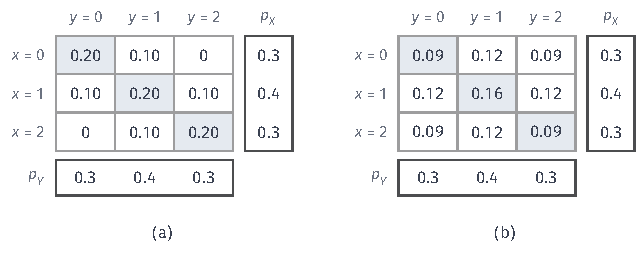
\includegraphics[width=108mm]{figures/07-probability/01-elementary-probability/tikz/rvc-same-marginals/figure.pdf}
  \caption{边缘相同、联合不同的两张概率表。(a)两台传感器的概率表。(b)每格取$p_X(x)p_Y(y)$得到的表。两表的行和与列和都是$(0.3,0.4,0.3)$；浅蓝格子组成事件$\{X=Y\}$，概率分别为$0.60$和$0.34$。}
  \label{fig:rvc-same-marginals}
\end{BookInlineFigure}

右表中读数一致的概率是
\[
 0.09+0.16+0.09=0.34,
\]
远小于左表的$0.60$；右表还允许一台读$0$、另一台读$2$，概率各为$0.09$。只看每台传感器各自的规律，分不出这两种情况。

连续情形也一样。对$\theta\in[-1,1]$，在单位正方形上令
\[
 f_{\theta}(x,y)=1+\theta(1-2x)(1-2y),\qquad 0\leq x,y\leq 1 .
\]
因为$\lvert(1-2x)(1-2y)\rvert\leq 1$，这个函数非负。对$y$积分时，$\int_{0}^{1}(1-2y)\,\mathrm{d}y=0$，所以
\[
 \int_{0}^{1}f_{\theta}(x,y)\,\mathrm{d}y=1+\theta(1-2x)\cdot 0=1 .
\]
同理对$x$积分也得$1$。于是每个$\theta$都给出一个联合密度，两个边缘都是$\operatorname{Unif}(0,1)$。图~\ref{fig:rvc-fgm}中，$\theta=1$时质量偏向两个分量同小或同大的角落，$\theta=-1$时偏向一小一大的角落。

\begin{BookInlineFigure}
  \centering
  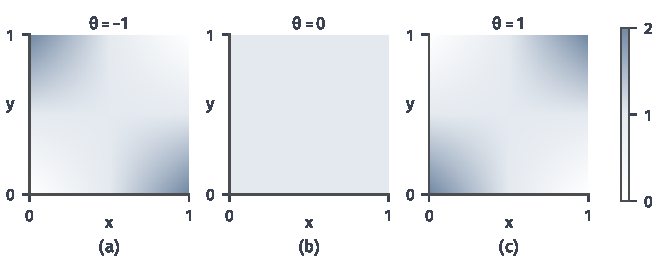
\includegraphics[width=112mm]{figures/07-probability/01-elementary-probability/matplotlib/rvc-fgm/figure.pdf}
  \caption{同样以$\operatorname{Unif}(0,1)$为两个边缘的三个联合密度$f_{\theta}(x,y)=1+\theta(1-2x)(1-2y)$。颜色由白到蓝表示密度由$0$到$2$。(a)$\theta=-1$。(b)$\theta=0$，密度处处为$1$。(c)$\theta=1$。}
  \label{fig:rvc-fgm}
\end{BookInlineFigure}

因此，单独知道每个分量的分布，不足以回答涉及几个分量共同取值的问题。联合分布在边缘之外还记录了分量之间的联系。下一节先研究联系“最弱”的情形：联合分布恰好可以由边缘拼出来。


\section{独立随机变量}
\label{sec:rvc-independence}

图~\ref{fig:rvc-same-marginals}(b)的表是用边缘“乘出来”的。什么时候真实的联合分布恰好就是这张乘积表？第~\ref{chap:classical-probability}章说过，两个事件独立，是指它们同时发生的概率等于各自概率之积。把这一要求加到由两个随机变量生成的每一对事件上，就得到随机变量的独立。

\paragraph{联合分布分解为边缘乘积}
第一台传感器读数落在某个范围，是一个事件；第二台读数落在某个范围，是另一个事件。如果知道其中一个的结果从来不改变另一个的概率，就说两台读数互不提供信息。下面的定义只对区间提出要求，区间可以是单点、有界区间或半直线。

\begin{definition}[独立随机变量]
\label{def:rvc-independence}
若对实数轴上的任意区间$A$和$B$都有
\begin{equation}
 \mathbb{P}(X\in A,\,Y\in B)=\mathbb{P}(X\in A)\,\mathbb{P}(Y\in B),
 \label{eq:rvc-independence}
\end{equation}
则称$X$与$Y$是\term{独立随机变量}（independent random variables），简称$X$与$Y$独立。
\end{definition}

取$A=(-\infty,x]$，$B=(-\infty,y]$，式~\eqref{eq:rvc-independence}给出$F_{X,Y}(x,y)=F_X(x)F_Y(y)$。反过来，若联合分布函数对一切$(x,y)$都分解为边缘分布函数之积，由式~\eqref{eq:rvc-rectangle}，每个半开矩形的概率都分解，独立性的其余情形可由这些矩形取极限得到，这一步留到第~\ref{chap:probability-spaces}章。实际计算中更常用的是下面针对概率表和密度的判别。

\begin{theorem}[独立性的判别]
\label{thm:rvc-independence-criterion}
\begin{enumerate}
 \item 若$X,Y$都只取有限个或可数个值，则$X$与$Y$独立，当且仅当对一切$x,y$，
 \begin{equation}
 p_{X,Y}(x,y)=p_X(x)\,p_Y(y).
 \label{eq:rvc-independence-pmf}
 \end{equation}
 \item 若$(X,Y)$有联合密度，$X,Y$分别有边缘密度$f_X,f_Y$，则$X$与$Y$独立，当且仅当乘积$f_X(x)f_Y(y)$也是$(X,Y)$的联合密度。特别地，若联合密度可以写成$f_{X,Y}(x,y)=g(x)h(y)$，其中$g,h$非负，则$X$与$Y$独立，并且
 \begin{equation}
 f_X=\frac{g}{\int g},\qquad f_Y=\frac{h}{\int h}.
 \label{eq:rvc-factorization}
 \end{equation}
\end{enumerate}
\end{theorem}

\begin{proof}
先看概率表。若$X,Y$独立，取单点区间$A=[x,x]$、$B=[y,y]$，式~\eqref{eq:rvc-independence}就是式~\eqref{eq:rvc-independence-pmf}。反过来，若式~\eqref{eq:rvc-independence-pmf}成立，对任意区间$A,B$，由式~\eqref{eq:rvc-joint-pmf-event}，
\[
 \mathbb{P}(X\in A,\,Y\in B)=\sum_{x\in A}\sum_{y\in B}p_X(x)\,p_Y(y).
\]
各项非负，二重和可以按任意顺序计算，先对$y$求和，得到
\[
 \sum_{x\in A}p_X(x)\sum_{y\in B}p_Y(y)=\mathbb{P}(X\in A)\,\mathbb{P}(Y\in B).
\]

再看密度。若$f_Xf_Y$是联合密度，对矩形$A\times B$，被积函数是$x$的函数与$y$的函数之积，累次积分分开计算：
\[
 \mathbb{P}(X\in A,\,Y\in B)=\int_{A}f_X(x)\,\mathrm{d}x\int_{B}f_Y(y)\,\mathrm{d}y=\mathbb{P}(X\in A)\,\mathbb{P}(Y\in B).
\]
无界区间按非负函数积分取极限理解。反过来，若$X,Y$独立，对每个矩形$R=A\times B$，
\[
 \iint_{R}f_X(x)f_Y(y)\,\mathrm{d}x\,\mathrm{d}y=\mathbb{P}(X\in A)\,\mathbb{P}(Y\in B)=\mathbb{P}\bigl((X,Y)\in R\bigr),
\]
这正是定义~\ref{def:rvc-joint-density}对联合密度的要求。

最后设$f_{X,Y}=gh$。由式~\eqref{eq:rvc-marginal-density}，$f_X(x)=g(x)\int h$，$f_Y(y)=h(y)\int g$；联合密度的总积分为$1$，即$\int g\int h=1$。于是
\[
 f_X(x)f_Y(y)=g(x)h(y)\int g\int h=g(x)h(y)=f_{X,Y}(x,y),
\]
由已证部分，$X$与$Y$独立，式~\eqref{eq:rvc-factorization}也同时得到。
\end{proof}

第二条说“乘积也是联合密度”，而不说“联合密度处处等于乘积”，是因为密度不唯一。把联合密度在一条直线上的值改掉，任何矩形上的积分都不变，改过的函数仍是联合密度，却可能在这条直线上不等于乘积。第~\ref{chap:probability-spaces}章会用“除去面积为零的集合”统一处理这类差别。

\paragraph{判别的例子}
两颗均匀骰子的点数$X_1,X_2$独立：每对点数的概率$1/36$恰好等于$\frac16\cdot\frac16$。同一试验中的$X$与$M$却不独立。由图~\ref{fig:rvc-dice-map}，
\[
 p_{X,M}(2,1)=0,\qquad p_X(2)\,p_M(1)=\frac16\cdot\frac1{36}>0 .
\]
只要找到一个格子不满足式~\eqref{eq:rvc-independence-pmf}，就足以否定独立。

两台传感器也不独立：$p_{X,Y}(0,2)=0$，而$p_X(0)p_Y(2)=0.09$。图~\ref{fig:rvc-same-marginals}(b)那张乘积表描述的才是“边缘相同而相互独立”的两台传感器。对照两张表可以看到，独立是对整张表的要求，九个格子都要分解。

连续情形里，单位正方形上的密度$f(x,y)=4xy$可以写成$(2x)(2y)$，所以两个分量独立，边缘密度都是$2t$，$0\leq t\leq 1$。三角形模型则不独立，理由可以直接从图上读出。取$A=[0,1/2)$，$B=(1/2,1]$，矩形$A\times B$整个落在三角形外，所以$\mathbb{P}(X<1/2,\,Y>1/2)=0$。而由两个边缘密度，
\[
 \mathbb{P}(X<\tfrac12)=\int_{0}^{1/2}2x\,\mathrm{d}x=\tfrac14,\qquad
 \mathbb{P}(Y>\tfrac12)=\int_{1/2}^{1}2(1-y)\,\mathrm{d}y=\tfrac14,
\]
乘积为$1/16\neq 0$。

这个论证给出一条常用的经验：若$X,Y$独立，联合质量只能分布在“$X$可能取的值”与“$Y$可能取的值”组成的乘积形区域上。三角形、圆盘这类不是乘积形的区域上的均匀分布，分量一定不独立。反之，区域是乘积形并不保证独立，图~\ref{fig:rvc-fgm}中$\theta\neq 0$的密度就是反例。

判别定理回答的是“给定联合分布，分量是否独立”。实际建模时常常反过来：两颗骰子分别掷出、两台仪器各自供电，物理上互不影响，于是\emph{假定}它们独立，再用定理~\ref{thm:rvc-independence-criterion}由边缘写出联合分布。这一假定是否合适，要回到试验本身判断；一旦假定错了，例如两台传感器其实受同一股气流影响，按乘积表算出的$\mathbb{P}(X=Y)=0.34$就会低估真实的$0.60$。

\paragraph{多个随机变量的独立}
传感器不止两台时，要求每一组读数范围的联合概率都分解。设$X_1,\dots,X_d$定义在同一样本空间上。若对任意区间$A_1,\dots,A_d$都有
\begin{equation}
 \mathbb{P}(X_1\in A_1,\dots,X_d\in A_d)=\prod_{i=1}^{d}\mathbb{P}(X_i\in A_i),
 \label{eq:rvc-mutual-independence}
\end{equation}
则称$X_1,\dots,X_d$\term{相互独立}（mutually independent）。取某些$A_i$为整个实数轴，这些因子变成$1$，所以任意一部分变量也相互独立。概率表和密度的判别与定理~\ref{thm:rvc-independence-criterion}相同：联合质量函数或联合密度分解为$d$个边缘之积。

只要求每两个变量独立，称为\term{两两独立}（pairwise independent），这比相互独立弱。令$X,Y$独立，各以概率$1/2$取$1$或$-1$，再令$Z=XY$。$(X,Y,Z)$只有四种等可能的取值，即图~\ref{fig:rvc-pairwise}中的四个实心点。

\begin{BookInlineFigure}
  \centering
  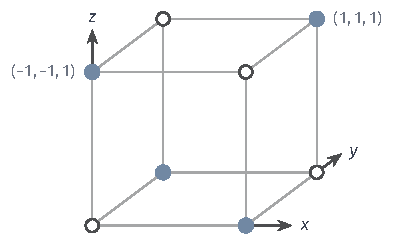
\includegraphics[width=67mm]{figures/07-probability/01-elementary-probability/tikz/rvc-pairwise/figure.pdf}
  \caption{两两独立但不相互独立。$X,Y$是独立的等可能符号，$Z=XY$。立方体八个角中，四个实心点满足$z=xy$，各有概率$1/4$；四个空心点的概率为零。从任一坐标方向把立方体压到一个面上，四个实心点恰好落在该面的四个角，每角$1/4$。}
  \label{fig:rvc-pairwise}
\end{BookInlineFigure}

先验证$X$与$Z$独立。$Z$等可能取$\pm1$。对任意$x,z\in\{1,-1\}$，事件$\{X=x,Z=z\}$就是$\{X=x,Y=xz\}$，于是
\[
 \mathbb{P}(X=x,\,Z=z)=\mathbb{P}(X=x)\,\mathbb{P}(Y=xz)=\tfrac14=\mathbb{P}(X=x)\,\mathbb{P}(Z=z).
\]
同理$Y$与$Z$独立，$X$与$Y$本来独立。三者却不相互独立：
\[
 \mathbb{P}(X=1,\,Y=1,\,Z=-1)=0\neq\tfrac18 .
\]
知道$X$和$Y$以后，$Z$完全确定；而单独知道其中任一个，对$Z$没有任何信息。

\paragraph{独立变量的函数}
传感器读数独立时，把读数换算成温度、取平方或截断，结果仍应独立。下面在概率表的情形证明这一点。设$X,Y$只取有限个或可数个值且独立，$g,h$是实函数。对任意区间$A,B$，令$G=\{x:g(x)\in A\}$，$H=\{y:h(y)\in B\}$，则
\[
 \begin{aligned}
 \mathbb{P}\bigl(g(X)\in A,\,h(Y)\in B\bigr)&=\sum_{x\in G}\sum_{y\in H}p_X(x)\,p_Y(y)\\
 &=\mathbb{P}\bigl(g(X)\in A\bigr)\,\mathbb{P}\bigl(h(Y)\in B\bigr).
 \end{aligned}
\]
所以$g(X)$与$h(Y)$独立。有密度时，集合$G,H$可能不再是区间，同样的结论需要第~\ref{chap:probability-spaces}章对一般集合的处理，这里直接使用。多个变量时结论同样成立：相互独立的变量分成互不相交的几组，各组的函数仍相互独立，例如$X_1+X_2$与$X_3^{2}$独立。

\paragraph{联合分布下的期望}
独立性最常用的推论是乘积的期望可以分开计算。先需要知道怎样对联合分布求期望。第~\ref{chap:random-variable-moments}章对一元情形说明，计算$\mathbb{E}[g(X)]$不必先求$g(X)$的分布。二元情形同样如此：在求和或积分绝对收敛时，
\begin{equation}
 \mathbb{E}\bigl[\varphi(X,Y)\bigr]=\sum_{x,y}\varphi(x,y)\,p_{X,Y}(x,y)
 \quad\text{或}\quad
 \iint\varphi(x,y)\,f_{X,Y}(x,y)\,\mathrm{d}x\,\mathrm{d}y .
 \label{eq:rvc-joint-expectation}
\end{equation}
概率表的情形，把取值对按$\varphi(x,y)$的值分组，同组质量之和就是$\varphi(X,Y)$取该值的概率，于是左右两边是同一个和的两种排列。密度的情形，$\varphi(X,Y)$可能既无概率表也无密度，它的期望及上式的证明要用第~\ref{chap:probability-spaces}章的积分，这里把上式当作计算规则使用。$d$维时把二元和、二重积分换成$d$元和、$d$重积分。

\begin{theorem}[独立变量乘积的期望]
\label{thm:rvc-product-expectation}
设$X$与$Y$独立，$\mathbb{E}\lvert g(X)\rvert<\infty$，$\mathbb{E}\lvert h(Y)\rvert<\infty$。则$g(X)h(Y)$的期望存在，并且
\begin{equation}
 \mathbb{E}\bigl[g(X)h(Y)\bigr]=\mathbb{E}\bigl[g(X)\bigr]\,\mathbb{E}\bigl[h(Y)\bigr].
 \label{eq:rvc-product-expectation}
\end{equation}
\end{theorem}

\begin{proof}
在概率表的情形，由定理~\ref{thm:rvc-independence-criterion}，联合质量等于$p_X(x)p_Y(y)$。先检查绝对收敛：非负项的二重和可以先对$y$求和，
\[
 \sum_{x,y}\lvert g(x)\rvert\,\lvert h(y)\rvert\,p_X(x)\,p_Y(y)
 =\Bigl(\sum_{x}\lvert g(x)\rvert p_X(x)\Bigr)\Bigl(\sum_{y}\lvert h(y)\rvert p_Y(y)\Bigr)<\infty .
\]
因此由式~\eqref{eq:rvc-joint-expectation}，$\mathbb{E}[g(X)h(Y)]$存在。绝对收敛的二重和同样可以先对$y$求和，去掉绝对值重复上面的计算，就得到式~\eqref{eq:rvc-product-expectation}。在密度的情形，取$f_Xf_Y$为联合密度，把求和换成积分：先对非负的$\lvert g(x)h(y)\rvert f_X(x)f_Y(y)$做累次积分，确认积分有限，再按绝对可积函数的累次积分规则分开计算。
\end{proof}

可积条件的作用是保证求和与积分的次序可以交换；只有两个期望都有限，右边的乘积才有意义。例如两颗骰子的点数之积，期望为$(7/2)^{2}=49/4$；$f=4xy$的模型中，
\[
 \mathbb{E}[XY]=\int_{0}^{1}\!\!\int_{0}^{1}xy\cdot 4xy\,\mathrm{d}x\,\mathrm{d}y=4\cdot\frac13\cdot\frac13=\frac49 ,
\]
恰好是$\mathbb{E}[X]^{2}=(2/3)^{2}$。

定理也可以反过来用于否定独立。三角形模型中$\mathbb{E}[X]=2/3$，$\mathbb{E}[Y]=1/3$，而
\[
 \mathbb{E}[XY]=\int_{0}^{1}\!\!\int_{0}^{x}2xy\,\mathrm{d}y\,\mathrm{d}x=\int_{0}^{1}x^{3}\,\mathrm{d}x=\frac14\neq\frac29 .
\]
但等式~\eqref{eq:rvc-product-expectation}只对一对特定的函数成立时，并不能推出独立，第~\ref{sec:rvc-moments}节会给出反例。

\paragraph{独立同分布}
重复试验的标准模型是：每次试验在相同条件下进行，各次结果互不影响。用随机变量写出来，就是下面的两个要求同时成立。若$X_1,\dots,X_n$相互独立，并且具有同一个分布$P$，则称它们\term{独立同分布}（independent and identically distributed），简记为i.i.d.，并写
\begin{equation}
 X_1,\dots,X_n\overset{\text{i.i.d.}}{\sim}P .
 \label{eq:rvc-iid}
\end{equation}
由定理~\ref{thm:rvc-independence-criterion}，它们的联合质量函数或联合密度是同一个边缘的$n$次乘积，例如$\prod_{i=1}^{n}p(x_i)$。

“同分布”只约束每个分量各自的规律，“独立”只约束分量之间的关系，两者谁也推不出谁。图~\ref{fig:rvc-iid}用两颗骰子说明三种情况。(a)两颗骰子独立掷出，$36$个格点各有$1/36$，两项都满足。(b)令$X_2=X_1$，两个分量同分布，但质量全在对角线上，不独立。(c)$X_1$是骰子点数，$X_2$是独立抛出的均匀硬币，记正面为$1$，两者独立但分布不同。

\begin{BookInlineFigure}
  \centering
  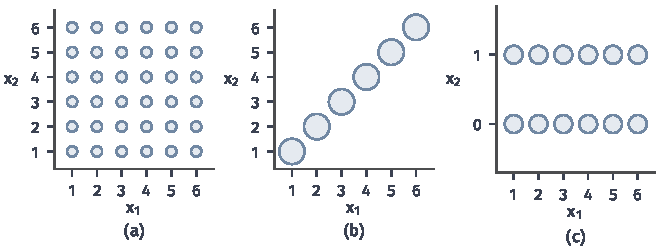
\includegraphics[width=112mm]{figures/07-probability/01-elementary-probability/matplotlib/rvc-iid/figure.pdf}
  \caption{独立与同分布是两项不同的要求，圆的面积正比于联合质量。(a)两颗独立的均匀骰子，每点$1/36$。(b)$X_2=X_1$，对角线上每点$1/6$：同分布，不独立。(c)骰子点数$X_1$与独立的均匀硬币$X_2\in\{0,1\}$，每点$1/12$：独立，不同分布。}
  \label{fig:rvc-iid}
\end{BookInlineFigure}

在(b)中，两次“试验”其实只做了一次，第二个数只是抄写第一个；在(c)中，两次试验互不影响，但做的不是同一种试验。只有(a)对应“同一试验独立重复两次”。后面讨论样本平均为什么随次数增加而稳定时，两项要求分别承担不同作用：同分布保证每次平均的是同一个量，独立保证波动能互相抵消，见第~\ref{chap:laws-of-large-numbers}章。


\section{均值与协方差}
\label{sec:rvc-moments}

把两台传感器的读数取平均，波动能减小多少？若两台独立，直觉告诉我们方差减半；可是图~\ref{fig:rvc-sensor-table}的两台读数倾向于一致，平均以后的改善应当少一些。要把“少多少”算出来，需要一个能概括两个量一起偏离中心的数。完整的联合分布在高维时难以列出，这一节用均值向量和协方差矩阵概括它的中心与波动。全节假定所涉及的各分量都有有限二阶矩，即$\mathbb{E}[X_i^{2}]<\infty$；只用到均值的地方，有限一阶矩就够了。

\paragraph{均值向量}
随机向量的中心可以逐个分量描述。设每个分量都有有限期望，定义\term{均值向量}（mean vector）
\begin{equation}
 \bm{\mu}=\mathbb{E}[\bm{X}]=\bigl(\mathbb{E}[X_1],\dots,\mathbb{E}[X_d]\bigr)^{\top}.
 \label{eq:rvc-mean-vector}
\end{equation}
一元时期望是质量分布的重心；这里$\bm{\mu}$是平面或空间中质量分布的重心。传感器表中$\bm{\mu}=(1,1)^{\top}$。三角形模型中，由边缘密度，
\[
 \mathbb{E}[X]=\int_{0}^{1}x\cdot 2x\,\mathrm{d}x=\frac23,\qquad \mathbb{E}[Y]=\int_{0}^{1}y\cdot 2(1-y)\,\mathrm{d}y=\frac13,
\]
$\bm{\mu}=(2/3,1/3)^{\top}$，正是三角形三个顶点坐标的平均，也就是均匀薄板的重心。

期望对随机向量是线性的。在式~\eqref{eq:rvc-joint-expectation}中取$\varphi(x,y)=x+y$，把和或积分拆成两项，得到$\mathbb{E}[X+Y]=\mathbb{E}[X]+\mathbb{E}[Y]$。逐行使用这一点，对$m\times d$常矩阵$\bm{A}$和常向量$\bm{b}\in\mathbb{R}^{m}$，
\begin{equation}
 \mathbb{E}[\bm{A}\bm{X}+\bm{b}]=\bm{A}\bm{\mu}+\bm{b}.
 \label{eq:rvc-mean-affine}
\end{equation}
这里不需要分量之间有任何独立性。矩阵按全书约定用粗体大写字母表示，后面的协方差矩阵$\bm{\Sigma}$也是如此。

\paragraph{协方差与交叉项}
和的均值只依赖各分量的均值，和的方差却不同。记$\mu_X=\mathbb{E}[X]$，$\mu_Y=\mathbb{E}[Y]$，把$X+Y$减去均值后平方展开：
\[
 \operatorname{Var}(X+Y)=\mathbb{E}\Bigl[\bigl((X-\mu_X)+(Y-\mu_Y)\bigr)^{2}\Bigr].
\]
平方展开成三项，再由期望的线性，
\[
 \operatorname{Var}(X+Y)=\operatorname{Var}(X)+\operatorname{Var}(Y)+2\,\mathbb{E}\bigl[(X-\mu_X)(Y-\mu_Y)\bigr].
\]
前两项只依赖边缘分布，最后一项依赖联合分布。这个交叉项就是我们要找的量。

\begin{definition}[协方差]
\label{def:rvc-covariance}
设$\mathbb{E}[X^{2}]<\infty$，$\mathbb{E}[Y^{2}]<\infty$。称
\begin{equation}
 \operatorname{Cov}(X,Y)=\mathbb{E}\bigl[(X-\mu_X)(Y-\mu_Y)\bigr]
 \label{eq:rvc-covariance}
\end{equation}
为$X$与$Y$的\term{协方差}（covariance）。
\end{definition}

有限二阶矩保证这个期望存在：由$\lvert uv\rvert\leq(u^{2}+v^{2})/2$，中心化乘积的绝对值被两个平方项之和控制。展开乘积并用线性，得到常用的计算公式
\begin{equation}
 \operatorname{Cov}(X,Y)=\mathbb{E}[XY]-\mu_X\mu_Y .
 \label{eq:rvc-covariance-formula}
\end{equation}

中心化乘积$(X-\mu_X)(Y-\mu_Y)$的符号有直观意义。以均值点$(\mu_X,\mu_Y)$为原点把平面分成四个象限：两个量同时偏高或同时偏低时，乘积为正；一高一低时，乘积为负。协方差把每个取值对的乘积按质量加权求和。为正，说明“同向偏离”的质量占优；为负，说明“反向偏离”占优。

图~\ref{fig:rvc-cov-quadrants}把传感器表的九个格子画成圆，并标出每格对协方差的贡献$(x-1)(y-1)p_{X,Y}(x,y)$。位于均值线上的格子贡献为零；四个角中，左下与右上各贡献$+0.20$，另两角的概率为零。于是
\[
 \operatorname{Cov}(X,Y)=0.20+0.20=0.40 .
\]
用式~\eqref{eq:rvc-covariance-formula}核对：$XY$只在$x,y\geq1$的四格非零，
\[
 \mathbb{E}[XY]=1\cdot0.20+2\cdot0.10+2\cdot0.10+4\cdot0.20=1.4,
\]
\[
 \operatorname{Cov}(X,Y)=1.4-1\cdot1=0.4 .
\]

\begin{BookInlineFigure}
  \centering
  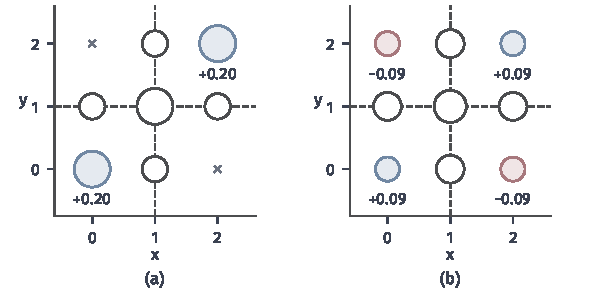
\includegraphics[width=100mm]{figures/07-probability/01-elementary-probability/matplotlib/rvc-cov-quadrants/figure.pdf}
  \caption{协方差是中心化乘积的加权和。圆的面积正比于格子的概率，虚线过均值$(1,1)$。蓝色格子的贡献$(x-1)(y-1)p_{X,Y}(x,y)$为正，红色为负，白色为零，叉号表示概率为零的格子；数字是各格的贡献。(a)传感器表，协方差$0.40$。(b)边缘相同的乘积表，正负贡献抵消，协方差为$0$。}
  \label{fig:rvc-cov-quadrants}
\end{BookInlineFigure}

协方差关于每个变量都是线性的，并且不受平移影响。由定义直接得到：对常数$a,b,c,e$，
\[
 \operatorname{Cov}(aX+b,\,cY+e)=ac\operatorname{Cov}(X,Y),\qquad \operatorname{Cov}(X,X)=\operatorname{Var}(X),
\]
并且对第三个二阶矩有限的变量$X_2$，
\[
 \operatorname{Cov}(X+X_2,\,Y)=\operatorname{Cov}(X,Y)+\operatorname{Cov}(X_2,Y).
\]把这些性质用于$\sum_i a_iX_i$与它自己，就得到有限和的方差展开：
\begin{equation}
 \operatorname{Var}\Bigl(\sum_{i=1}^{n}a_iX_i\Bigr)=\sum_{i=1}^{n}a_i^{2}\operatorname{Var}(X_i)+2\sum_{i<j}a_ia_j\operatorname{Cov}(X_i,X_j).
 \label{eq:rvc-variance-sum}
\end{equation}
$n$个对角项来自各分量自身的波动，$n(n-1)/2$个交叉项来自两两之间的共同波动。

用传感器表算一算。由式~\eqref{eq:rvc-variance-sum}，
\[
 \operatorname{Var}(X+Y)=0.6+0.6+2\cdot0.4=2.0 .
\]
直接核对：把表中格子按$x+y$的值分组，$X+Y$在$\{0,1,2,3,4\}$上各取概率$0.2$，均值为$2$，方差为$(4+1+0+1+4)\times0.2=2$。两台读数的平均$(X+Y)/2$方差为$2.0/4=0.5$，只比单台的$0.6$小一点；若换成图~\ref{fig:rvc-same-marginals}(b)那样独立的两台，交叉项为零，平均的方差是$1.2/4=0.3$，正好减半。

交叉项的符号随系数而变。两台读数之差的方差是
\[
 \operatorname{Var}(X-Y)=0.6+0.6-2\cdot0.4=0.4 .
\]
直接核对：$X-Y$以概率$0.6$取$0$，以概率$0.2$各取$\pm1$，方差为$0.4$。正相关使和的波动变大、差的波动变小，所以比较两台读数之差，比单看一台更容易发现某台失灵：正常时差几乎总在$0$附近。

\paragraph{协方差矩阵}
$d$个分量两两之间都有协方差，排成矩阵便于统一计算。定义\term{协方差矩阵}（covariance matrix）
\begin{equation}
 \bm{\Sigma}=\operatorname{Cov}(\bm{X})=\mathbb{E}\bigl[(\bm{X}-\bm{\mu})(\bm{X}-\bm{\mu})^{\top}\bigr],\qquad
 \bm{\Sigma}_{i,j}=\operatorname{Cov}(X_i,X_j),
 \label{eq:rvc-covariance-matrix}
\end{equation}
其中矩阵的期望逐个元素计算。对角元是各分量的方差，非对角元是协方差。传感器表和三角形模型的协方差矩阵分别是
\[
 \begin{bmatrix}0.6&0.4\\0.4&0.6\end{bmatrix},\qquad
 \begin{bmatrix}1/18&1/36\\1/36&1/18\end{bmatrix}.
\]
后者由边缘密度算出$\mathbb{E}[X^{2}]=1/2$、$\mathbb{E}[Y^{2}]=1/6$，再用上一节的$\mathbb{E}[XY]=1/4$：
\[
 \operatorname{Var}(X)=\tfrac12-\tfrac49=\tfrac1{18},\quad
 \operatorname{Var}(Y)=\tfrac16-\tfrac19=\tfrac1{18},\quad
 \operatorname{Cov}(X,Y)=\tfrac14-\tfrac29=\tfrac1{36}.
\]

式~\eqref{eq:rvc-variance-sum}写成矩阵形式，就是协方差矩阵最重要的性质。

\begin{theorem}[协方差矩阵的性质]
\label{thm:rvc-covariance-matrix}
设$\bm{X}$的各分量有有限二阶矩，协方差矩阵为$\bm{\Sigma}$。对常向量$\bm{a},\bm{b}\in\mathbb{R}^{d}$，
\begin{equation}
 \operatorname{Cov}(\bm{a}^{\top}\bm{X},\,\bm{b}^{\top}\bm{X})=\bm{a}^{\top}\bm{\Sigma}\bm{b},\qquad
 \operatorname{Var}(\bm{a}^{\top}\bm{X})=\bm{a}^{\top}\bm{\Sigma}\bm{a}\geq 0 .
 \label{eq:rvc-quadratic-form}
\end{equation}
因此$\bm{\Sigma}$对称半正定。对$m\times d$常矩阵$\bm{A}$和常向量$\bm{b}\in\mathbb{R}^{m}$，
\begin{equation}
 \operatorname{Cov}(\bm{A}\bm{X}+\bm{b})=\bm{A}\bm{\Sigma}\bm{A}^{\top}.
 \label{eq:rvc-covariance-affine}
\end{equation}
\end{theorem}

\begin{proof}
协方差的定义关于两个变量对称，所以$\bm{\Sigma}$对称。由式~\eqref{eq:rvc-mean-affine}，$\bm{a}^{\top}\bm{X}$的均值是$\bm{a}^{\top}\bm{\mu}$，所以它的中心化是$\bm{a}^{\top}(\bm{X}-\bm{\mu})$；$\bm{b}^{\top}\bm{X}$同理。两个标量之积可以写成
\[
 \bigl(\bm{a}^{\top}(\bm{X}-\bm{\mu})\bigr)\bigl(\bm{b}^{\top}(\bm{X}-\bm{\mu})\bigr)
 =\bm{a}^{\top}(\bm{X}-\bm{\mu})(\bm{X}-\bm{\mu})^{\top}\bm{b}.
\]
右边是矩阵元素的线性组合，取期望时可以逐项进行，得到$\bm{a}^{\top}\bm{\Sigma}\bm{b}$。取$\bm{b}=\bm{a}$，左边是方差，必不小于零，这对一切$\bm{a}$成立，所以$\bm{\Sigma}$半正定。最后，$\bm{A}\bm{X}+\bm{b}$的第$i$个分量是$\bm{A}_{i,:}\bm{X}+b_i$，常数不影响协方差，由第一式，它与第$j$个分量的协方差为$\bm{A}_{i,:}\bm{\Sigma}\bm{A}_{j,:}^{\top}$，这正是$\bm{A}\bm{\Sigma}\bm{A}^{\top}$的$(i,j)$元。
\end{proof}

用式~\eqref{eq:rvc-covariance-affine}可以一次算出几个线性组合的全部方差与协方差。对传感器读数取平均$Z=(X+Y)/2$与差$W=X-Y$，即
\[
 \begin{bmatrix}Z\\W\end{bmatrix}=\bm{A}\begin{bmatrix}X\\Y\end{bmatrix},\qquad
 \bm{A}=\begin{bmatrix}1/2&1/2\\1&-1\end{bmatrix}.
\]
矩阵相乘得到
\[
 \bm{A}\bm{\Sigma}\bm{A}^{\top}
 =\begin{bmatrix}1/2&1/2\\1&-1\end{bmatrix}\begin{bmatrix}0.6&0.4\\0.4&0.6\end{bmatrix}\begin{bmatrix}1/2&1\\1/2&-1\end{bmatrix}
 =\begin{bmatrix}0.5&0\\0&0.4\end{bmatrix}.
\]
对角元与前面分别算出的$0.5$、$0.4$一致；非对角元为零，说明平均与差不相关。原因是两台读数方差相等：由协方差的双线性，交叉的两项互相抵消，
\[
 \operatorname{Cov}(Z,W)=\tfrac12\bigl(\operatorname{Var}(X)-\operatorname{Var}(Y)\bigr)=0 .
\]不相关并不等于独立，例如$W=\pm1$时$Z$只能取$1/2$或$3/2$，而$W=0$时$Z$可以取$0,1,2$。

式~\eqref{eq:rvc-quadratic-form}给协方差矩阵一个几何解释。取单位向量$\bm{a}$，$\bm{a}^{\top}(\bm{X}-\bm{\mu})$是点$\bm{X}$在方向$\bm{a}$上相对重心的有向距离，所以$\bm{a}^{\top}\bm{\Sigma}\bm{a}$是质量沿方向$\bm{a}$的散开程度。把概率看作质量，这正是力学中薄板绕“过重心且垂直于$\bm{a}$的直线”的转动惯量；一元方差是它的一维特例。

$\bm{\Sigma}$是实对称矩阵，可以正交对角化，单位特征向量给出散开程度最大和最小的方向，对应的特征值就是沿这些方向的方差，可参考\BookChapterRef{chap:eigen-spectral-decomposition}{卷二第6章“谱分解”}。三角形模型中，取$\bm{a}=(\cos\varphi,\sin\varphi)^{\top}$，
\[
 v(\varphi)=\bm{a}^{\top}\bm{\Sigma}\bm{a}=\frac{1}{18}+\frac{\sin 2\varphi}{36}.
\]
$\varphi=\pi/4$时取最大值$1/12$，方向$(1,1)^{\top}/\sqrt2$；$\varphi=3\pi/4$时取最小值$1/36$，方向$(1,-1)^{\top}/\sqrt2$。两者正是$\bm{\Sigma}$的两个特征值和特征向量，见图~\ref{fig:rvc-cov-ellipse}。

\begin{BookInlineFigure}
  \centering
  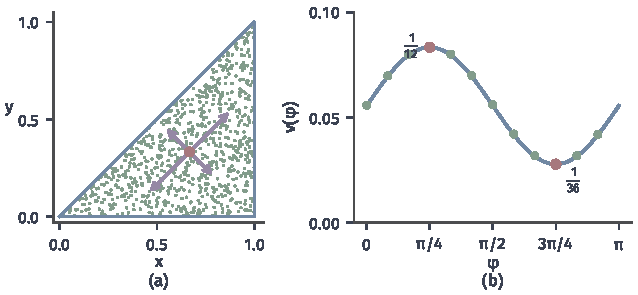
\includegraphics[width=108mm]{figures/07-probability/01-elementary-probability/matplotlib/rvc-cov-ellipse/figure.pdf}
  \caption{协方差矩阵与散开方向。(a)三角形模型的$800$个模拟点（绿，种子$1$），红点为均值$(2/3,1/3)$，紫色双箭头沿两个特征向量，半长等于该方向的标准差$\sqrt{1/12}$与$\sqrt{1/36}$。(b)方向$(\cos\varphi,\sin\varphi)$上的方差$v(\varphi)$（蓝线），红点为最大值与最小值，绿点是同一批模拟点投影后的样本方差。}
  \label{fig:rvc-cov-ellipse}
\end{BookInlineFigure}

半正定而不正定时，存在非零$\bm{a}$使$\bm{a}^{\top}\bm{\Sigma}\bm{a}=0$。这时$\bm{a}^{\top}\bm{X}$的方差为零，由第~\ref{chap:tail-probabilities}章的Chebyshev不等式，对每个$\varepsilon>0$，
\[
 \mathbb{P}\bigl(\lvert\bm{a}^{\top}\bm{X}-\bm{a}^{\top}\bm{\mu}\rvert\geq\varepsilon\bigr)\leq\frac{0}{\varepsilon^{2}}=0 .
\]
也就是说，$\bm{X}$偏离超平面$\bm{a}^{\top}\bm{x}=\bm{a}^{\top}\bm{\mu}$任何正距离的概率都是零，质量全部压在这个超平面上。例如把传感器读数排成$\bm{X}=(X,Y,X+Y)^{\top}$，由式~\eqref{eq:rvc-covariance-affine}，
\[
 \bm{\Sigma}=\begin{bmatrix}0.6&0.4&1.0\\0.4&0.6&1.0\\1.0&1.0&2.0\end{bmatrix},\qquad
 \bm{\Sigma}\begin{bmatrix}1\\1\\-1\end{bmatrix}=\bm{0}.
\]
零特征值对应的方向$(1,1,-1)^{\top}$正好表达了第三个分量等于前两个之和。这种由线性约束造成的奇异协方差，在第~\ref{chap:multivariate-distributions}章的计数向量中还会遇到。

\paragraph{相关系数}
协方差的数值依赖单位：把温度从摄氏度换成另一种刻度，乘以常数$c$，协方差也乘以$c$，而两台传感器之间的联系并没有改变。除以两个标准差，就得到与单位无关的量。

\begin{definition}[相关系数]
\label{def:rvc-correlation}
设$0<\operatorname{Var}(X)<\infty$，$0<\operatorname{Var}(Y)<\infty$，记$\sigma_X,\sigma_Y$为标准差。称
\begin{equation}
 \rho_{X,Y}=\frac{\operatorname{Cov}(X,Y)}{\sigma_X\sigma_Y}
 \label{eq:rvc-correlation}
\end{equation}
为$X$与$Y$的\term{相关系数}（correlation coefficient），不致混淆时简写为$\rho$。
\end{definition}

\begin{theorem}[相关系数的范围]
\label{thm:rvc-correlation-bound}
在上述条件下$-1\leq\rho_{X,Y}\leq 1$。若$\rho_{X,Y}=\pm1$，记
\begin{equation}
 L=\mu_Y+\rho_{X,Y}\frac{\sigma_Y}{\sigma_X}(X-\mu_X),
 \label{eq:rvc-correlation-line}
\end{equation}
则对每个$\varepsilon>0$有$\mathbb{P}(\lvert Y-L\rvert\geq\varepsilon)=0$。反过来，若$Y=a+bX$，$b\neq0$，则$\rho_{X,Y}$等于$b$的符号。
\end{theorem}

\begin{proof}
把两个变量标准化，令$U=(X-\mu_X)/\sigma_X$，$V=(Y-\mu_Y)/\sigma_Y$，则
\[
 \mathbb{E}[U^{2}]=\mathbb{E}[V^{2}]=1,\qquad \mathbb{E}[UV]=\rho .
\]
考虑非负随机变量$(V-\rho U)^{2}$，展开后取期望：
\[
 0\leq\mathbb{E}\bigl[(V-\rho U)^{2}\bigr]=\mathbb{E}[V^{2}]-2\rho\,\mathbb{E}[UV]+\rho^{2}\mathbb{E}[U^{2}]=1-\rho^{2},
\]
所以$\rho^{2}\leq1$。

若$\rho^{2}=1$，上式说明$\mathbb{E}[(V-\rho U)^{2}]=0$。对每个$\delta>0$，由第~\ref{chap:tail-probabilities}章的Markov不等式，
\[
 \mathbb{P}\bigl(\lvert V-\rho U\rvert\geq\delta\bigr)=\mathbb{P}\bigl((V-\rho U)^{2}\geq\delta^{2}\bigr)\leq\frac{0}{\delta^{2}}=0 .
\]
由式~\eqref{eq:rvc-correlation-line}，$\sigma_Y(V-\rho U)=Y-L$，取$\delta=\varepsilon/\sigma_Y$即得结论。

反过来，若$Y=a+bX$，则$\operatorname{Cov}(X,Y)=b\sigma_X^{2}$，$\sigma_Y=\lvert b\rvert\sigma_X$，代入式~\eqref{eq:rvc-correlation}得$\rho=b/\lvert b\rvert$。
\end{proof}

这个证明与内积空间中的Cauchy--Schwarz不等式是同一个论证：把$\mathbb{E}[UV]$看作两个中心化变量的内积，相关系数就是它们夹角的余弦，可参考\BookChapterRef{chap:inner-product-spaces}{卷二第4章“内积空间”}。定理的第二部分只说$Y$偏离直线$L$任何正距离的概率为零；第~\ref{chap:probability-spaces}章会说明这等价于$\mathbb{P}(Y=L)=1$。

两个贯穿例子的相关系数是
\[
 \rho_{\text{传感器}}=\frac{0.4}{\sqrt{0.6\cdot0.6}}=\frac23,\qquad
 \rho_{\text{三角形}}=\frac{1/36}{\sqrt{(1/18)(1/18)}}=\frac12 .
\]
对图~\ref{fig:rvc-fgm}的密度族，两个边缘的均值都是$1/2$，密度中的常数项$1$对应独立部分，贡献的协方差为零，于是
\[
 \operatorname{Cov}(X,Y)=\theta\Bigl(\int_{0}^{1}x(1-2x)\,\mathrm{d}x\Bigr)^{2}=\theta\Bigl(-\frac16\Bigr)^{2}=\frac{\theta}{36}.
\]
边缘方差为$1/12$，所以$\rho=\theta/3$，绝对值不超过$1/3$：这个族只能表达较弱的联系。

相关系数衡量的是散点向一条直线集中的程度，而不是直线的斜率。图~\ref{fig:rvc-correlation}前三幅中，$\rho=0.9$的点紧贴上升直线，$\rho=-0.6$的点较松散地沿下降方向分布，$\rho=0$的点看不出线性趋势。第四幅中$Y$几乎由$X$决定，相关系数却为零：抛物线左右两支对“同向”和“反向”的贡献互相抵消。

\begin{BookInlineFigure}
  \centering
  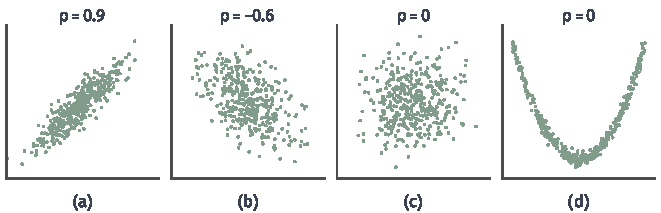
\includegraphics[width=112mm]{figures/07-probability/01-elementary-probability/matplotlib/rvc-correlation/figure.pdf}
  \caption{不同相关系数下的散点，每幅$400$个模拟点（种子$7$）。(a)至(c)中$X,Y$都服从$\mathcal{N}(0,1)$，取$Y=\rho X+\sqrt{1-\rho^{2}}\,Z$，$Z\sim\mathcal{N}(0,1)$与$X$独立，相关系数分别为$0.9$、$-0.6$、$0$。(d)中$X\sim\operatorname{Unif}(-\sqrt3,\sqrt3)$，$Y=X^{2}-1+0.1Z$，相关系数为$0$。}
  \label{fig:rvc-correlation}
\end{BookInlineFigure}

“集中于直线的程度”可以精确表述。用直线$a+bX$近似$Y$，以均方误差$\mathbb{E}[(Y-a-bX)^{2}]$衡量好坏。对固定的$b$，记$W=Y-bX$。把$W-a$拆成$(W-\mathbb{E}[W])+(\mathbb{E}[W]-a)$，交叉项的期望为零，于是
\[
 \mathbb{E}\bigl[(W-a)^{2}\bigr]=\operatorname{Var}(W)+\bigl(\mathbb{E}[W]-a\bigr)^{2}.
\]
最好的$a$是$\mathbb{E}[W]$，剩下的误差是
\[
 \operatorname{Var}(Y-bX)=\operatorname{Var}(Y)-2b\operatorname{Cov}(X,Y)+b^{2}\operatorname{Var}(X).
\]
这是$b$的二次函数，对$b$求导并令导数为零，最小点是
\[
 b^{*}=\frac{\operatorname{Cov}(X,Y)}{\operatorname{Var}(X)}.
\]
代回得到最小均方误差
\begin{equation}
 \min_{a,b}\mathbb{E}\bigl[(Y-a-bX)^{2}\bigr]=\operatorname{Var}(Y)\,(1-\rho_{X,Y}^{2}).
 \label{eq:rvc-best-line}
\end{equation}
所以$\rho^{2}$是最佳直线能解释的那一部分方差。$\rho=0$时最佳斜率为零，直线对预测$Y$毫无帮助；但这只说明直线无用，曲线仍可能很有用，图~\ref{fig:rvc-correlation}(d)就是这样。

\paragraph{平均能把波动降低多少}
现在回答本节开头的问题。设$n$台传感器的读数$X_1,\dots,X_n$方差都是$\sigma^{2}$，任意两台的相关系数都是$\rho$，即协方差都是$\rho\sigma^{2}$。由式~\eqref{eq:rvc-variance-sum}，取$a_i=1/n$，对角项共$n$个，交叉项共$n(n-1)/2$个，
\[
 \operatorname{Var}(\bar{X}_n)=\frac{1}{n^{2}}\Bigl(n\sigma^{2}+n(n-1)\rho\sigma^{2}\Bigr),
\]
其中$\bar{X}_n=(X_1+\dots+X_n)/n$。整理得
\begin{equation}
 \operatorname{Var}(\bar{X}_n)=\sigma^{2}\Bigl(\frac1n+\Bigl(1-\frac1n\Bigr)\rho\Bigr).
 \label{eq:rvc-equicorrelated-average}
\end{equation}

两台传感器的情形，$n=2$，$\sigma^{2}=0.6$，$\rho=2/3$，代入得$0.6\times(1/2+1/3)=0.5$，与前面直接计算的结果一致。$\rho=0$时上式变成$\sigma^{2}/n$，平均$n$次把方差降为$1/n$。$\rho>0$时，$n\to\infty$，方差趋于$\rho\sigma^{2}$而不是零：各台共有的那部分波动，例如同一股气流同时影响所有传感器，无论平均多少台都消不掉。

\begin{BookInlineFigure}
  \centering
  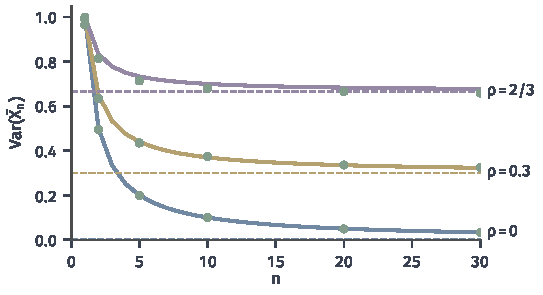
\includegraphics[width=92mm]{figures/07-probability/01-elementary-probability/matplotlib/rvc-average-variance/figure.pdf}
  \caption{$n$个方差为$1$、两两相关系数为$\rho$的读数，其平均的方差。实线是式~\eqref{eq:rvc-equicorrelated-average}，蓝、黄、紫分别对应$\rho=0,0.3,2/3$；虚线是极限$\rho$。绿点是$4000$次模拟的样本方差（种子$11$），每次取$X_i=\sqrt{\rho}\,Z_0+\sqrt{1-\rho}\,Z_i$，$Z_0,Z_1,\dots$相互独立且服从$\mathcal{N}(0,1)$。}
  \label{fig:rvc-average-variance}
\end{BookInlineFigure}

图~\ref{fig:rvc-average-variance}中，模拟用的构造$X_i=\sqrt{\rho}\,Z_0+\sqrt{1-\rho}\,Z_i$把每个读数拆成共同部分$Z_0$和各自部分$Z_i$。平均时各自部分的方差按$1/n$缩小，共同部分原样保留，这正是式~\eqref{eq:rvc-equicorrelated-average}两项的来源。

\paragraph{相关与独立}
协方差为零的两个变量称为\term{不相关}（uncorrelated）。独立变量一定不相关：若$X,Y$独立且二阶矩有限，在定理~\ref{thm:rvc-product-expectation}中取$g(x)=x-\mu_X$，$h(y)=y-\mu_Y$，得到
\[
 \operatorname{Cov}(X,Y)=\mathbb{E}[X-\mu_X]\,\mathbb{E}[Y-\mu_Y]=0 .
\]
因此两两独立的变量之和，方差等于方差之和；式~\eqref{eq:rvc-variance-sum}只需要交叉项为零，也就是只需要两两不相关。

反过来不成立，因为协方差只检查一种特定的乘积。令$X$等可能取$-1,0,1$，$Y=X^{2}$。则$\mathbb{E}[X]=0$，$\mathbb{E}[XY]=\mathbb{E}[X^{3}]=0$，所以$\operatorname{Cov}(X,Y)=0$。可是$Y$完全由$X$决定，独立性不成立：
\[
 \mathbb{P}(X=0,\,Y=1)=0\neq\mathbb{P}(X=0)\,\mathbb{P}(Y=1)=\tfrac13\cdot\tfrac23 .
\]

连续的例子是单位圆盘上的均匀分布，密度在圆盘内为$1/\pi$。把$(x,y)$换成$(-x,y)$，密度不变而$xy$变号，所以$\mathbb{E}[XY]=-\mathbb{E}[XY]=0$；同理$\mathbb{E}[X]=0$，协方差为零。圆盘不是乘积形区域，按上一节的判别，两个分量不独立。具体地，$\mathbb{P}(X>0.9)$与$\mathbb{P}(Y>0.5)$都为正，而点$(x,y)$满足$x>0.9$、$y>0.5$时$x^{2}+y^{2}>0.81+0.25>1$，落在圆盘外，所以$\mathbb{P}(X>0.9,\,Y>0.5)=0$。

\begin{BookInlineFigure}
  \centering
  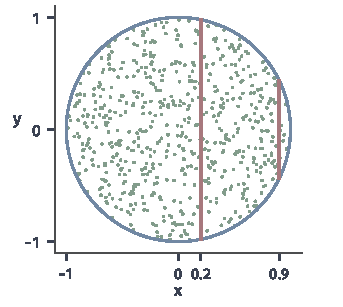
\includegraphics[width=58mm]{figures/07-probability/01-elementary-probability/matplotlib/rvc-disk/figure.pdf}
  \caption{单位圆盘上的均匀分布：不相关但不独立。绿点是$600$个模拟点（种子$3$），样本相关系数约为$-0.01$。红线段是$x=0.2$与$x=0.9$处$y$能取到的范围，分别为$\lvert y\rvert\leq0.98$和$\lvert y\rvert\leq0.44$。}
  \label{fig:rvc-disk}
\end{BookInlineFigure}

图~\ref{fig:rvc-disk}显示了依赖的方式：$X$靠近$\pm1$时，$Y$被挤到$0$附近，$X$靠近$0$时，$Y$可以取到$\pm1$附近。依赖体现在$Y$的散开程度随$X$改变，而不是$Y$的平均位置随$X$线性升降，协方差看不见这种依赖。表~\ref{tab:rvc-dependence}汇总本节的几个关系。

\begin{BookInlineTable}
  \centering
  \caption{独立、不相关与完全线性相关}
  \label{tab:rvc-dependence}
  \begin{tabular}{lll}
    \toprule
    关系 & 要求 & 可以推出 \\
    \midrule
    独立 & 联合分布分解为边缘之积 & 函数仍独立；有矩时不相关 \\
    不相关 & $\operatorname{Cov}(X,Y)=0$ & 和的方差等于方差之和 \\
    $\rho=\pm1$ & 达到相关系数的界 & $Y$偏离某条直线的概率为零 \\
    \bottomrule
  \end{tabular}
\end{BookInlineTable}

表中第一行到第二行只有单向的箭头；零相关只排除线性关联，不排除依赖。在多元高斯模型中，不相关与独立恰好等价，那是第~\ref{chap:multivariate-distributions}章的一个特殊结论，不能推广到一般分布。


\section{条件分布的计算}
\label{sec:rvc-conditional}

第一台传感器读到$0$，第二台会读什么？已经知道$X=0$，所有$X\neq0$的样本点都被排除，剩下的只有概率表的第一行。第~\ref{chap:classical-probability}章的条件概率正是这样做的：缩小样本范围，再把剩下的质量重新归一，使总和回到$1$。这一节把这个操作用到联合分布上，先在概率表中计算，再处理密度，最后用条件分布计算条件均值，并把总方差拆成两部分。

\paragraph{概率表中的条件分布}
设$p_X(x)>0$。由条件概率的定义，
\[
 \mathbb{P}(Y=y\mid X=x)=\frac{\mathbb{P}(X=x,\,Y=y)}{\mathbb{P}(X=x)}.
\]
把它看作$y$的函数，记
\begin{equation}
 p_{Y\mid X}(y\mid x)=\frac{p_{X,Y}(x,y)}{p_X(x)},\qquad p_X(x)>0 ,
 \label{eq:rvc-conditional-pmf}
\end{equation}
称为给定$X=x$时$Y$的\term{条件质量函数}（conditional probability mass function），它确定的分布称为给定$X=x$时$Y$的\term{条件分布}（conditional distribution）。对固定的$x$，分子按$y$求和恰好是分母，所以条件质量函数非负且和为$1$，是一个正常的概率表。

在概率表上，这就是取出第$x$行，再除以该行之和。传感器表的三行之和分别为$0.3,0.4,0.3$，得到
\[
 p_{Y\mid X}(\cdot\mid 0)=\bigl(\tfrac23,\tfrac13,0\bigr),\quad
 p_{Y\mid X}(\cdot\mid 1)=\bigl(\tfrac14,\tfrac12,\tfrac14\bigr),\quad
 p_{Y\mid X}(\cdot\mid 2)=\bigl(0,\tfrac13,\tfrac23\bigr).
\]
第一台读$0$时，第二台不可能读$2$；第一台读$1$时，第二台的读数对称地分布在$1$两侧。三行的形状互不相同，见图~\ref{fig:rvc-conditional-pmf}。

\begin{BookInlineFigure}
  \centering
  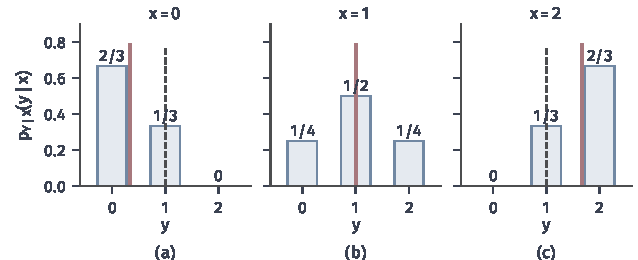
\includegraphics[width=108mm]{figures/07-probability/01-elementary-probability/matplotlib/rvc-conditional-pmf/figure.pdf}
  \caption{传感器表中给定第一台读数时第二台读数的条件分布。(a)、(b)、(c)分别对应$x=0,1,2$，柱高为$p_{Y\mid X}(y\mid x)$；红线是条件均值$1/3$、$1$、$5/3$，虚线是不加条件时的均值$1$。}
  \label{fig:rvc-conditional-pmf}
\end{BookInlineFigure}

把式~\eqref{eq:rvc-conditional-pmf}两边乘以$p_X(x)$，得到联合质量的另一种写法：
\begin{equation}
 p_{X,Y}(x,y)=p_X(x)\,p_{Y\mid X}(y\mid x).
 \label{eq:rvc-multiplication}
\end{equation}
它说明联合分布可以分两步给出：先按$p_X$定下$X$的值，再按该值对应的条件分布定下$Y$。许多模型正是这样描述的，先说明一个量怎样产生，再说明另一个量在前者给定时怎样产生。对$x$求和就是第~\ref{chap:classical-probability}章的全概率公式，
\[
 p_Y(y)=\sum_{x}p_X(x)\,p_{Y\mid X}(y\mid x),
\]
其中$p_X(x)=0$的项本来就是零，可以略去。反过来求给定$Y=y$时$X$的条件分布，就是Bayes公式：当$p_Y(y)>0$时，
\[
 p_{X\mid Y}(x\mid y)=\frac{p_X(x)\,p_{Y\mid X}(y\mid x)}{p_Y(y)}.
\]
传感器表关于对角线对称，例如$p_{X\mid Y}(0\mid 0)=0.3\cdot\frac23/0.3=\frac23$，与$p_{Y\mid X}(0\mid 0)$相同。

\paragraph{给连续变量取条件}
三角形模型中，若已知$X=0.6$，$Y$怎样分布？困难在于$\mathbb{P}(X=0.6)=0$，式~\eqref{eq:rvc-conditional-pmf}的分母为零。自然的办法是先以一个有正概率的窄带代替这个点：给定$x\leq X\leq x+h$，再让$h\to0$，见图~\ref{fig:rvc-conditional-slices}(a)。

设$f_{X,Y}$在$x$附近连续，且$f_X(x)>0$。窄带上的条件概率是两个积分之比，
\[
 \mathbb{P}(Y\leq y\mid x\leq X\leq x+h)
 =\frac{\int_{x}^{x+h}\int_{-\infty}^{y}f_{X,Y}(s,t)\,\mathrm{d}t\,\mathrm{d}s}{\int_{x}^{x+h}f_X(s)\,\mathrm{d}s}.
\]
分子分母同除以$h$。窄带越来越窄时，两者分别趋于被积函数在$s=x$处的值，于是
\[
 \lim_{h\to0}\mathbb{P}(Y\leq y\mid x\leq X\leq x+h)=\int_{-\infty}^{y}\frac{f_{X,Y}(x,t)}{f_X(x)}\,\mathrm{d}t .
\]
右边被积的函数正是窄带极限下$Y$的密度。

\begin{definition}[条件密度]
\label{def:rvc-conditional-density}
设$(X,Y)$有联合密度$f_{X,Y}$，$X$的边缘密度为$f_X$。对满足$f_X(x)>0$的$x$，定义
\begin{equation}
 f_{Y\mid X}(y\mid x)=\frac{f_{X,Y}(x,y)}{f_X(x)},
 \label{eq:rvc-conditional-density}
\end{equation}
称为给定$X=x$时$Y$的\term{条件密度}（conditional density）。
\end{definition}

和概率表一样，条件密度是联合密度沿竖线$\{X=x\}$的切片，除以切片的总积分$f_X(x)$而得到；它对$y$的积分为$1$。三角形模型中，对$0<x\leq1$有$f_X(x)=2x>0$，切片在$0\leq y\leq x$上取值$2$，所以
\[
 f_{Y\mid X}(y\mid x)=\frac{2}{2x}=\frac1x,\qquad 0\leq y\leq x .
\]
给定$X=x$时，$Y$服从$\operatorname{Unif}(0,x)$：均匀分布的点落在竖线上，只能落在三角形内的那一段，并且在这一段上没有偏好。

\begin{BookInlineFigure}
  \centering
  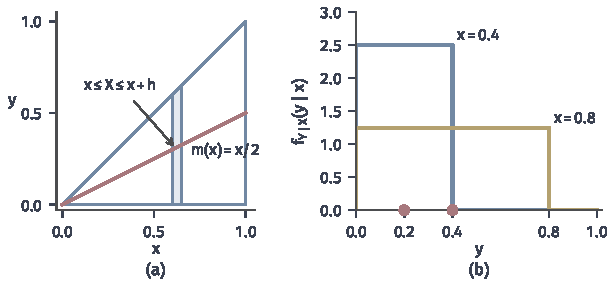
\includegraphics[width=104mm]{figures/07-probability/01-elementary-probability/matplotlib/rvc-conditional-slices/figure.pdf}
  \caption{三角形模型的条件化。(a)浅蓝窄带是事件$\{x\leq X\leq x+h\}$，$x=0.6$，$h=0.05$；红线是条件均值$m(x)=x/2$。(b)给定$X=0.4$（蓝）与$X=0.8$（黄）时$Y$的条件密度，分别是高$2.5$与$1.25$的矩形；红点是两个条件均值$0.2$与$0.4$。}
  \label{fig:rvc-conditional-slices}
\end{BookInlineFigure}

式~\eqref{eq:rvc-conditional-density}只在$f_X(x)>0$处使用。另一个限制更隐蔽：联合密度可以在一条竖线$\{x=x_0\}$上任意改动而不改变任何概率，改动后$f_{Y\mid X}(\cdot\mid x_0)$就变了。所以单独一个$x_0$处的条件密度并不由联合分布决定；只有把各个$x$处的条件密度合起来使用，例如对$x$积分，结果才有确定的意义。条件于零概率事件的严格含义，以及不同的取极限方式可能给出不同答案的现象，在第~\ref{chap:conditional-distributions}章说明。

有了条件密度，式~\eqref{eq:rvc-multiplication}和全概率公式都有连续版本：在$f_X(x)>0$处$f_{X,Y}(x,y)=f_X(x)f_{Y\mid X}(y\mid x)$，并且
\[
 f_Y(y)=\int f_X(x)\,f_{Y\mid X}(y\mid x)\,\mathrm{d}x,
\]
积分只在$f_X(x)>0$的范围进行。对三角形模型，$\int_{y}^{1}2x\cdot\frac1x\,\mathrm{d}x=2(1-y)$，与第~\ref{sec:rvc-joint}节直接求出的$f_Y$相同。

反方向的条件化同样计算。给定$Y=y$，$0\leq y<1$，由$f_Y(y)=2(1-y)>0$，
\[
 f_{X\mid Y}(x\mid y)=\frac{2}{2(1-y)}=\frac{1}{1-y},\qquad y\leq x\leq 1 ,
\]
即$X$在给定$Y=y$时服从$\operatorname{Unif}(y,1)$：较小的读数已知为$y$，较大的读数在$y$与$1$之间没有偏好。横线与竖线上的切片都是均匀的，但切片的位置与长度随条件改变，这正是两个分量不独立的表现。

\paragraph{条件分布与独立}
独立性可以换一种方式理解：知道$X$的值不改变$Y$的分布。在概率表的情形，由式~\eqref{eq:rvc-independence-pmf}与式~\eqref{eq:rvc-conditional-pmf}，$X,Y$独立当且仅当对每个满足$p_X(x)>0$的$x$，
\[
 p_{Y\mid X}(y\mid x)=p_Y(y)\quad\text{对一切}\ y\ \text{成立}.
\]
条件分布与$x$无关，各行重新归一以后长得一样。传感器表的三行形状各异，再次说明两台读数不独立。

有密度时，若$X,Y$独立，取$f_Xf_Y$为联合密度，条件密度就是$f_Y$，同样与$x$无关。图~\ref{fig:rvc-slices}比较了两个连续模型：$f=4xy$的条件密度在三个$x$处完全重合，都是$2y$；三角形模型的条件密度是宽度为$x$的矩形，随$x$改变。

\begin{BookInlineFigure}
  \centering
  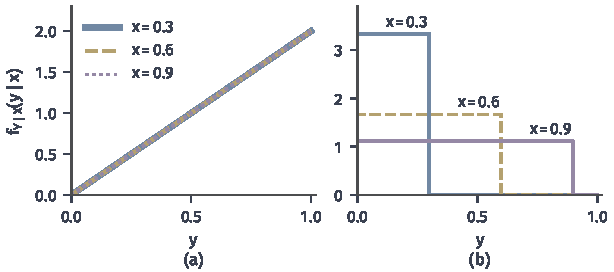
\includegraphics[width=104mm]{figures/07-probability/01-elementary-probability/matplotlib/rvc-slices/figure.pdf}
  \caption{独立就是条件分布不随条件改变。蓝、黄、紫分别对应$x=0.3,0.6,0.9$。(a)单位正方形上的密度$4xy$，三条条件密度重合为$2y$。(b)三角形模型，条件密度是$[0,x]$上高为$1/x$的矩形。}
  \label{fig:rvc-slices}
\end{BookInlineFigure}

\paragraph{离散状态与连续读数}
条件变量与被条件变量不必同属一类。设房间有两种状态：$X=0$表示正常，$X=1$表示过热，$\mathbb{P}(X=1)=0.2$。正常时一台精确传感器的读数$Y$服从$\mathcal{N}(20,1)$，过热时服从$\mathcal{N}(23,1)$。这里$X$有概率表，$Y$在给定$X$时有密度，联合规律由式~\eqref{eq:rvc-multiplication}的两步方式给出：
\begin{equation}
 \mathbb{P}(X=x,\,Y\in B)=p_X(x)\int_{B}f_{Y\mid X}(y\mid x)\,\mathrm{d}y .
 \label{eq:rvc-mixed-joint}
\end{equation}

对$x$求和，$Y$的边缘密度是两个高斯密度的加权和。记$\phi(z)=\mathrm{e}^{-z^{2}/2}/\sqrt{2\pi}$为标准高斯密度，则
\[
 f_Y(y)=0.8\,\phi(y-20)+0.2\,\phi(y-23).
\]
这种由若干分布按权重相加得到的分布称为\term{混合分布}（mixture distribution）。图~\ref{fig:rvc-mixture}(a)中，蓝线是$f_Y$，主峰来自正常状态，右侧的肩来自过热状态。

\begin{BookInlineFigure}
  \centering
  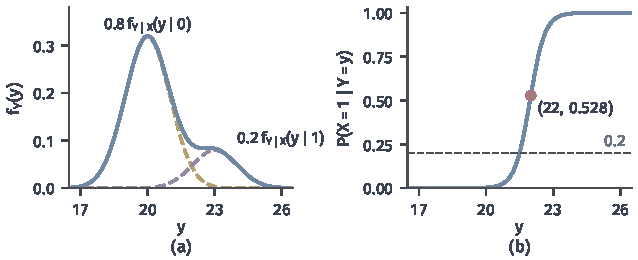
\includegraphics[width=108mm]{figures/07-probability/01-elementary-probability/matplotlib/rvc-mixture/figure.pdf}
  \caption{离散状态与连续读数。$\mathbb{P}(X=1)=0.2$，给定$X=0$与$X=1$时$Y$分别服从$\mathcal{N}(20,1)$与$\mathcal{N}(23,1)$。(a)蓝线为$Y$的密度，黄、紫虚线为两部分$0.8\,\phi(y-20)$与$0.2\,\phi(y-23)$。(b)读到$y$以后过热的条件概率，虚线是不加条件时的概率$0.2$，红点为$y=22$。}
  \label{fig:rvc-mixture}
\end{BookInlineFigure}

读到$Y=y$以后，过热的可能性有多大？$\mathbb{P}(Y=y)=0$，仍用窄带$y\leq Y\leq y+h$取极限，由式~\eqref{eq:rvc-mixed-joint}，分子分母同除以$h$后得到Bayes公式的密度形式：
\begin{equation}
 \mathbb{P}(X=1\mid Y=y)=\frac{p_X(1)\,f_{Y\mid X}(y\mid 1)}{f_Y(y)} .
 \label{eq:rvc-mixed-bayes}
\end{equation}
取$y=22$，两部分分别含$\phi(-1)$与$\phi(2)$，约去$1/\sqrt{2\pi}$，
\[
 \mathbb{P}(X=1\mid Y=22)=\frac{0.2\,\mathrm{e}^{-1/2}}{0.2\,\mathrm{e}^{-1/2}+0.8\,\mathrm{e}^{-2}}
 =\frac{1}{1+4\mathrm{e}^{-3/2}}\approx0.528 .
\]
读数$22$离过热状态的中心更近，过热的概率从$0.2$升到一半以上。取$y=21.5$时，两部分的指数相同，比值回到先验权重：$\mathbb{P}(X=1\mid Y=21.5)=0.2$，这个读数不提供区分两种状态的信息。

\paragraph{条件均值}
条件分布确定以后，可以像一元情形一样求它的期望。设$\mathbb{E}\lvert Y\rvert<\infty$，并且下面的和或积分有限，定义
\begin{equation}
 m(x)=\mathbb{E}[Y\mid X=x]=\sum_{y}y\,p_{Y\mid X}(y\mid x)\quad\text{或}\quad\int y\,f_{Y\mid X}(y\mid x)\,\mathrm{d}y ,
 \label{eq:rvc-conditional-mean}
\end{equation}
称为给定$X=x$时$Y$的\term{条件均值}（conditional mean）。它是“只看$X=x$那一组”时$Y$的平均，即组内平均。

传感器表中，由三行条件分布，
\[
 m(0)=\tfrac13,\qquad m(1)=1,\qquad m(2)=\tfrac53 ,
\]
可以合写为$m(x)=1/3+2x/3$。三角形模型中$Y$在给定$X=x$时服从$\operatorname{Unif}(0,x)$，$m(x)=x/2$。有趣的是，两个例子中$m$恰好都等于式~\eqref{eq:rvc-best-line}的最佳直线$\mu_Y+b^{*}(x-\mu_X)$：传感器表中$b^{*}=0.4/0.6=2/3$，三角形模型中$b^{*}=(1/36)/(1/18)=1/2$。一般情形下条件均值不必是直线，它作为最佳预测的含义在第~\ref{chap:conditional-expectation}章说明。

把$x$换成随机的$X$，得到随机变量$m(X)$，记作$\mathbb{E}[Y\mid X]$。它的值随$X$的值而定：传感器表中，$\mathbb{E}[Y\mid X]$以概率$0.3,0.4,0.3$取$1/3,1,5/3$。它的期望回到$Y$的期望，这就是下面的\term{全期望公式}（law of total expectation）。

\begin{theorem}[全期望公式]
\label{thm:rvc-total-expectation}
设$\mathbb{E}\lvert Y\rvert<\infty$，$X$有概率表或$(X,Y)$有联合密度。则
\begin{equation}
 \mathbb{E}[Y]=\mathbb{E}\bigl[\mathbb{E}[Y\mid X]\bigr]=\sum_{x}m(x)\,p_X(x)\quad\text{或}\quad\int m(x)\,f_X(x)\,\mathrm{d}x .
 \label{eq:rvc-total-expectation}
\end{equation}
\end{theorem}

\begin{proof}
在概率表的情形，由式~\eqref{eq:rvc-multiplication}，
\[
 \sum_{x}p_X(x)\,m(x)=\sum_{x}p_X(x)\sum_{y}y\,p_{Y\mid X}(y\mid x)=\sum_{x,y}y\,p_{X,Y}(x,y).
\]
条件$\mathbb{E}\lvert Y\rvert<\infty$保证二重和绝对收敛，求和可以按任意分组进行，右边就是$\mathbb{E}[Y]$。在密度的情形，把求和换成积分，并在$f_X(x)>0$处使用$f_{X,Y}=f_Xf_{Y\mid X}$。
\end{proof}

全期望公式就是“总平均等于各组平均的加权平均”，权重是各组的质量。传感器表中，
\[
 0.3\cdot\tfrac13+0.4\cdot1+0.3\cdot\tfrac53=0.1+0.4+0.5=1=\mathbb{E}[Y].
\]
三角形模型中，两个方向的条件均值分别是$m(x)=x/2$与$\mathbb{E}[X\mid Y=y]=(1+y)/2$，代入全期望公式，
\[
 \mathbb{E}[Y]=\frac{\mathbb{E}[X]}{2}=\frac13,\qquad \mathbb{E}[X]=\frac{1+\mathbb{E}[Y]}{2}=\frac23,
\]
都与边缘密度算出的结果一致。混合模型中$\mathbb{E}[Y]=0.8\cdot20+0.2\cdot23=20.6$。

\paragraph{全方差公式}
条件分布也有方差。设$\mathbb{E}[Y^{2}]<\infty$，在概率表的情形定义
\begin{equation}
 v(x)=\operatorname{Var}(Y\mid X=x)=\sum_{y}\bigl(y-m(x)\bigr)^{2}p_{Y\mid X}(y\mid x),
 \label{eq:rvc-conditional-variance}
\end{equation}
称为给定$X=x$时$Y$的\term{条件方差}（conditional variance）；密度的情形把和换成积分。它是组内的散开程度。$Y$的总方差与它有什么关系？回答是下面的\term{全方差公式}（law of total variance）。

\begin{theorem}[全方差公式]
\label{thm:rvc-total-variance}
设$\mathbb{E}[Y^{2}]<\infty$，$X$有概率表或$(X,Y)$有联合密度。则
\begin{equation}
 \operatorname{Var}(Y)=\mathbb{E}\bigl[v(X)\bigr]+\operatorname{Var}\bigl(m(X)\bigr).
 \label{eq:rvc-total-variance}
\end{equation}
\end{theorem}

\begin{proof}
记$\mu_Y=\mathbb{E}[Y]$，在概率表的情形证明。固定满足$p_X(x)>0$的$x$，把$y-\mu_Y$拆成$(y-m(x))+(m(x)-\mu_Y)$，在条件分布下求平方的平均。交叉项含有$\sum_{y}(y-m(x))p_{Y\mid X}(y\mid x)$，由$m(x)$的定义它等于零，于是
\[
 \sum_{y}(y-\mu_Y)^{2}p_{Y\mid X}(y\mid x)=v(x)+\bigl(m(x)-\mu_Y\bigr)^{2}.
\]
两边乘以$p_X(x)$再对$x$求和。由式~\eqref{eq:rvc-multiplication}，左边成为
\[
 \sum_{x,y}(y-\mu_Y)^{2}p_{X,Y}(x,y)=\operatorname{Var}(Y).
\]右边第一项是$\mathbb{E}[v(X)]$；由全期望公式$\mathbb{E}[m(X)]=\mu_Y$，第二项是$\operatorname{Var}(m(X))$。密度的情形逐字把求和换成积分。
\end{proof}

证明中的第一个等式是力学中的平行轴定理：质量对任意一点的二阶矩，等于对自身重心的二阶矩加上重心偏移的平方。式~\eqref{eq:rvc-total-variance}于是读作：总波动等于组内波动的平均，加上各组平均之间的波动。

三个例子逐一核对。传感器表中三行的条件方差为$2/9,1/2,2/9$，$m(X)=1/3+2X/3$，所以
\[
 \mathbb{E}[v(X)]=0.3\cdot\tfrac29+0.4\cdot\tfrac12+0.3\cdot\tfrac29=\tfrac13,\qquad
 \operatorname{Var}\bigl(m(X)\bigr)=\bigl(\tfrac23\bigr)^{2}\cdot0.6=\tfrac{4}{15},
\]
两者之和为$9/15=0.6=\operatorname{Var}(Y)$。三角形模型中$v(x)=x^{2}/12$，$m(X)=X/2$，
\[
 \mathbb{E}[v(X)]=\frac{\mathbb{E}[X^{2}]}{12}=\frac{1}{24},\qquad
 \operatorname{Var}\bigl(m(X)\bigr)=\frac{\operatorname{Var}(X)}{4}=\frac{1}{72},
\]
和为$1/18$。混合模型中两组的方差都是$1$，组平均$20$与$23$以权重$0.8,0.2$分布，组间方差为$3^{2}\times0.8\times0.2=1.44$，所以$\operatorname{Var}(Y)=1+1.44=2.44$。

由式~\eqref{eq:rvc-total-variance}，$\mathbb{E}[v(X)]\leq\operatorname{Var}(Y)$：平均而言，知道$X$以后$Y$的不确定性不会增加。但这只对平均成立，个别条件可以让波动变大。单位圆盘的均匀分布中，$\operatorname{Var}(Y)=\mathbb{E}[Y^{2}]=1/4$，而给定$X=0$时$Y$服从$\operatorname{Unif}(-1,1)$，条件方差为$1/3$；圆盘中央那条竖线比整个圆盘在竖直方向更“长”。

本节的计算都针对给定的具体取值$x$，结果是$x$的普通函数。把条件均值当作随机变量来研究，例如它为什么是在已知$X$时对$Y$的最佳预测、在什么意义下唯一，属于第~\ref{chap:conditional-expectation}章；没有概率表也没有密度时怎样定义条件分布，属于第~\ref{chap:conditional-distributions}章。


\section{本章小结}
\label{sec:rvc-summary}

本章从两台传感器的问题出发：两台同时报偏高的概率、一台读数已知时另一台的规律、平均以后的波动，都要求知道几个量在同一次观测中怎样共同取值。把定义在同一样本空间上的随机变量排成随机向量，这份共同规律就是联合分布。离散时它是一张概率表，连续时是单位面积上的质量即联合密度，两类模型都可以用联合分布函数描述，矩形概率由四个角上的值确定。

从联合分布出发，本章得到的几种对象可以放在同一张概率表上看。表~\ref{tab:rvc-summary}按传感器表列出它们的算法与结果。

\begin{BookInlineTable}
  \centering
  \caption{从联合分布得到的对象（传感器表）}
  \label{tab:rvc-summary}
  \begin{tabular}{lll}
    \toprule
    对象 & 在概率表上的操作 & 结果 \\
    \midrule
    边缘分布 & 按行、按列求和 & $(0.3,0.4,0.3)$ \\
    独立性 & 每格与边缘之积比较 & 不独立 \\
    均值向量 & 按质量加权平均 & $(1,1)^{\top}$ \\
    协方差 & 中心化乘积加权求和 & $0.4$ \\
    条件分布 & 取出一行，除以行和 & 如$(\tfrac23,\tfrac13,0)$ \\
    条件均值 & 对每行求均值 & $\tfrac13+\tfrac23x$ \\
    \bottomrule
  \end{tabular}
\end{BookInlineTable}

边缘化把其余分量的信息汇总掉，不能逆转：相同的边缘可以对应许多不同的联合分布。只有在独立时，联合分布才由边缘拼成乘积；判别时，概率表要求每个格子分解，密度要求边缘乘积本身就是联合密度。独立带来两项计算上的便利：乘积的期望可以分开计算（两个期望有限时），条件分布不随条件改变。独立同分布同时要求同分布与相互独立，两项不能互相替代；两两独立也不足以推出相互独立。

均值向量是质量分布的重心，协方差矩阵描述质量沿各个方向的散开程度。它对称半正定，$\bm{a}^{\top}\bm{\Sigma}\bm{a}$是$\bm{a}^{\top}\bm{X}$的方差，奇异时质量压在一个超平面上。有限和的方差展开中，交叉项来自分量之间的协方差，它决定平均能把波动降低多少：各读数方差同为$\sigma^{2}$、两两相关系数同为$\rho>0$时，无论平均多少个读数，方差都降不到$\rho\sigma^{2}$以下。相关系数介于$-1$与$1$之间，衡量向一条直线集中的程度；独立推出不相关，反之不成立，零相关只排除线性关联。

条件分布在概率表中是取出一行再重新归一，在密度中是取一条切片再除以$f_X(x)$，只在分母为正时使用。条件均值是组内平均，全期望公式说总平均是组平均的加权平均，全方差公式把总方差分成组内方差的平均与组平均之间的方差。单个零概率条件下的条件密度不由联合分布唯一确定，严格的处理在第~\ref{chap:conditional-distributions}章完成。

下一章用这些结构考察具体的多元模型：多项计数的和为常数，造成奇异协方差；多元高斯分布由均值向量和协方差矩阵完全确定；共同尺度可以让不相关的分量仍然相互依赖。按给定联合分布实际产生样本以及效率问题，在第~\ref{chap:sample-generation}章展开。


\chapter{常见多元分布}
\label{chap:multivariate-distributions}

一家甜品店有三种口味，记下接连四位顾客各选了哪一种，得到三个计数；从装着三种颜色小球的盒子里一次摸出四个，也得到三个计数。两台传感器同时测量同一个房间，给出两个可正可负的误差。一份混合物由三种成分组成，三个比例都在$0$与$1$之间，加起来恰好是$1$。这些记录都是随机向量，第~\ref{chap:random-vectors}章已经准备好了描述它们的一般语言：联合分布、边缘、条件、均值向量与协方差矩阵。

可是一般语言不告诉我们具体的概率应当是多少。四位顾客的口味计数取$(2,1,1)$的机会有多大？两台传感器的误差为什么常常一起变大？三个比例能不能各自独立地随机取值？要回答这些问题，需要从试验机制或取值范围出发，写出具体的联合分布，再看它的参数各管什么，分量之间的依赖从哪里来。

本章的五个模型分成三类。计数模型的总数固定，分量之间必然相关，独立重复与不放回抽样又给出不同的协方差。实值观测从多元高斯出发：它由均值向量和协方差矩阵完全确定，边缘、条件和独立性都能用这两个参数直接算出；把它的固定尺度换成所有分量共用的随机尺度，就得到尾部更重的多元t分布和多元Laplace分布。组成比例由Dirichlet分布描述，它住在比例之和为$1$的三角形或更高维单纯形上。

这些模型反复用到同一个问题：知道了每个分量的分布，甚至知道了协方差，能否断定分量之间独立？我们会看到，计数的总和约束、高斯的仿射结构、共同尺度和比例的归一化，各自以不同方式回答它。最后一节把五个模型并排比较。随机变量经过一般映射后的分布、密度换元的完整依据，在第~\ref{chap:random-variable-transformations}章统一处理。

\section{计数分布}
\label{sec:mvd-counting}

先看最朴素的多元记录：每次观察落入$d$个类别之一，观察$n$次，数每一类出现了几次。结果是一个整数向量$\bm{N}=(N_1,\ldots,N_d)^{\top}$，分量非负，并且
\[
 N_1+N_2+\cdots+N_d=n .
\]
这条等式对每一次试验结果都成立，不是平均意义下成立。

本节用两个场景贯穿。第一个是甜品店：每位顾客独立地选口味，选第$1,2,3$种的概率分别是$0.5,0.3,0.2$，记录四位顾客。第二个是摸球：盒子里有$10$个球，其中红球$5$个、绿球$3$个、黄球$2$个，一次不放回地摸出$4$个。两个场景中每一类所占的比例相同，都是$(0.5,0.3,0.2)$，计数总和都是$4$。区别只在一处：顾客之间互不影响，而摸出一个红球会改变盒中剩余的组成。

总和固定这一点已经告诉我们，分量不可能相互独立：若$N_1=4$，其余分量只能是$0$。下面先由试验机制推出两种联合分布，再用示性变量算出它们的均值与协方差，看总和约束和抽样方式分别在协方差里留下什么痕迹。

\subsection{多项分布}
\label{sec:mvd-multinomial}

\paragraph{联合质量函数}
设一个试验重复$n$次，各次相互独立；每次恰好落入$d$个类别之一，落入第$i$类的概率是$p_i$，各次相同。这里$p_i\geq0$，$p_1+\cdots+p_d=1$，记$\bm{p}=(p_1,\ldots,p_d)^{\top}$。用$N_i$表示$n$次中落入第$i$类的次数。

要算$\bm{N}$取某个$\bm{k}=(k_1,\ldots,k_d)^{\top}$的概率，可以先看一条具体的结果序列。例如四位顾客依次选了口味$1,3,1,2$，由独立性，这条序列的概率是各次概率之积，
\[
 p_1\cdot p_3\cdot p_1\cdot p_2=p_1^{2}p_2p_3 .
\]
它只依赖每一类出现了几次，与出现的先后无关。所以$\bm{N}=\bm{k}$的概率等于“计数为$\bm{k}$的序列条数”乘以$\prod_ip_i^{k_i}$。

把$n$个位置分给$d$个类别，第$i$类占$k_i$个位置，分法的数目是多项式系数$n!/(k_1!\cdots k_d!)$：先把$n$个位置全排列，再除去每一类内部位置互换造成的重复。这一计数可参考\BookChapterRef{chap:counting}{卷一第2章“计数”}。合起来得到下面的定义。

\begin{definition}[多项分布]
\label{def:mvd-multinomial}
设$n$为正整数，$\bm{p}$的分量非负且和为$1$。若随机向量$\bm{N}$满足
\begin{equation}
 \mathbb{P}(\bm{N}=\bm{k})=\frac{n!}{k_1!\,k_2!\cdots k_d!}\,p_1^{k_1}p_2^{k_2}\cdots p_d^{k_d},
 \label{eq:mvd-multinomial-pmf}
\end{equation}
其中$\bm{k}$取遍满足$k_i\geq0$、$k_1+\cdots+k_d=n$的整数向量，则称$\bm{N}$服从参数为$n$与$\bm{p}$的\term{多项分布}（multinomial distribution），记为$\bm{N}\sim\operatorname{Mult}(n,\bm{p})$。
\end{definition}

式~\eqref{eq:mvd-multinomial-pmf}的各项之和为$1$，因为按多项式定理，它们恰好是$(p_1+\cdots+p_d)^{n}=1$的展开。$d=2$时，$N_2=n-N_1$由$N_1$决定，式~\eqref{eq:mvd-multinomial-pmf}就是二项分布的质量函数。

回到甜品店，$n=4$，$\bm{p}=(0.5,0.3,0.2)^{\top}$。计数$(2,1,1)$的系数是$4!/(2!\,1!\,1!)=12$，于是
\[
 \mathbb{P}\bigl(\bm{N}=(2,1,1)\bigr)=12\times0.5^{2}\times0.3\times0.2=0.18 .
\]
四位顾客全选第$1$种的概率是$0.5^{4}=0.0625$，全选第$3$种的概率只有$0.2^{4}=0.0016$。

这些概率全部住在一个三角形格点集上。三个计数之和为$4$，可能的取值共有$15$个，把它们画成等边三角形里的格点，三个顶点分别是$(4,0,0)$、$(0,4,0)$和$(0,0,4)$。图~\ref{fig:mvd-count-lattice}(a)用圆的面积表示概率：质量集中在靠近$(2,1,1)$的地方，也就是靠近$n\bm{p}=(2,1.2,0.8)$的地方。三维向量只在一个二维的格点三角形上取值，这正是总和约束的几何形状。

\begin{BookInlineFigure}
  \centering
  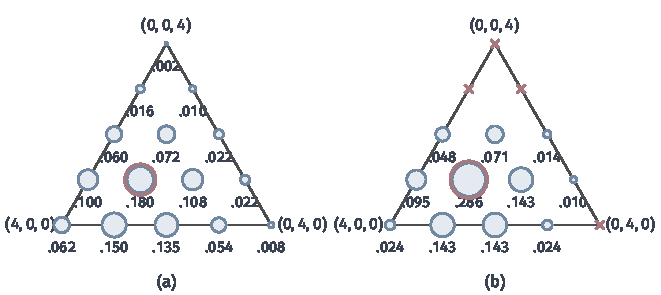
\includegraphics[width=112mm]{figures/07-probability/01-elementary-probability/matplotlib/mvd-count-lattice/figure.pdf}
  \caption{总和为$4$的三类计数的联合分布，每个格点代表一个计数向量$(k_1,k_2,k_3)$，圆的面积与概率成正比，下方数字是概率。(a)多项分布$\operatorname{Mult}(4,(0.5,0.3,0.2))$。(b)从$5$红、$3$绿、$2$黄共$10$个球中不放回摸$4$个的多元超几何分布；红叉是不可能出现的计数。红圈标出$(2,1,1)$。}
  \label{fig:mvd-count-lattice}
\end{BookInlineFigure}

\paragraph{合并类别与边缘分布}
只关心第$1$类时，可以把其余类别合成“非第$1$类”。每次试验仍然相互独立，落入第$1$类的概率仍是$p_1$，所以$N_1$就是$n$次独立试验中的成功次数：
\[
 N_i\sim\operatorname{Bin}(n,p_i),\qquad i=1,\ldots,d .
\]
更一般地，把若干类别合并成一类，合并后的计数仍服从多项分布，参数是对应概率之和。例如甜品店中把口味$1,2$合并，
\[
 (N_1+N_2,\ N_3)\sim\operatorname{Mult}\bigl(4,(0.8,0.2)\bigr) .
\]
这种做法不需要对式~\eqref{eq:mvd-multinomial-pmf}求和，它直接回到试验机制：合并类别只是把记录方式变粗，独立重复的结构没有改变。

\paragraph{示性变量与协方差}
计数的均值和协方差最好通过逐次记录来算。对第$t$次试验和第$i$类，令示性变量
\[
 I_{t,i}=\mathbf{1}_{\{\text{第}t\text{次落入第}i\text{类}\}},\qquad N_i=\sum_{t=1}^{n}I_{t,i} .
\]
把$I_{t,i}$排成$n$行$d$列的表，图~\ref{fig:mvd-indicator-table}画出了序列$1,3,1,2$对应的表，列和就是计数。

\begin{BookInlineFigure}
  \centering
  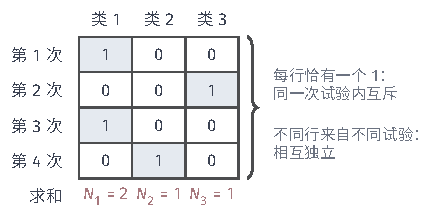
\includegraphics[width=73mm]{figures/07-probability/01-elementary-probability/tikz/mvd-indicator-table/figure.pdf}
  \caption{四次试验、三个类别的示性变量表，对应结果序列$1,3,1,2$。每一行恰有一个$1$（浅蓝），各列之和给出计数$\bm{N}=(2,1,1)$。同一行内的示性变量互斥，不同行来自相互独立的试验。}
  \label{fig:mvd-indicator-table}
\end{BookInlineFigure}

表中有两种关系。同一行的$d$个示性变量互斥：一次试验只能落入一个类别，所以$i\neq j$时$I_{t,i}I_{t,j}=0$。不同行来自不同试验，相互独立。前者产生负的协方差，后者不产生任何交叉项。

\begin{theorem}[多项计数的均值与协方差]
\label{thm:mvd-multinomial-moments}
设$\bm{N}\sim\operatorname{Mult}(n,\bm{p})$，则$\mathbb{E}[\bm{N}]=n\bm{p}$，并且
\begin{equation}
 \operatorname{Cov}(N_i,N_j)=
 \begin{cases}
  np_i(1-p_i), & i=j,\\
  -np_ip_j, & i\neq j .
 \end{cases}
 \label{eq:mvd-multinomial-cov}
\end{equation}
用矩阵写，即
\begin{equation}
 \operatorname{Cov}(\bm{N})=n\bigl(\operatorname{diag}(\bm{p})-\bm{p}\bm{p}^{\top}\bigr) .
 \label{eq:mvd-multinomial-cov-matrix}
\end{equation}
\end{theorem}

\begin{proof}
每个$I_{t,i}$只取$0,1$，取$1$的概率是$p_i$，所以$\mathbb{E}[I_{t,i}]=p_i$，对$t$求和得$\mathbb{E}[N_i]=np_i$。

协方差对两个变量都是线性的，展开两个和式，
\[
 \operatorname{Cov}(N_i,N_j)=\sum_{t=1}^{n}\sum_{s=1}^{n}\operatorname{Cov}(I_{t,i},I_{s,j}) .
\]
$t\neq s$时两个示性变量来自不同试验，相互独立，协方差为$0$。只剩$t=s$的$n$项。

同一次试验中，$i=j$时$I_{t,i}^{2}=I_{t,i}$；$i\neq j$时$I_{t,i}I_{t,j}=0$。于是
\[
 \operatorname{Cov}(I_{t,i},I_{t,j})=\mathbb{E}[I_{t,i}I_{t,j}]-p_ip_j=
 \begin{cases}
  p_i-p_i^{2}, & i=j,\\
  -p_ip_j, & i\neq j .
 \end{cases}
\]
乘以$n$即得式~\eqref{eq:mvd-multinomial-cov}。
\end{proof}

对甜品店，$n=4$，$\bm{p}=(0.5,0.3,0.2)^{\top}$，代入式~\eqref{eq:mvd-multinomial-cov}，协方差矩阵是
\[
 \begin{bmatrix}
  1 & -0.6 & -0.4\\
  -0.6 & 0.84 & -0.24\\
  -0.4 & -0.24 & 0.64
 \end{bmatrix} .
\]
对角元是三个二项分布的方差，非对角元全为负：一位顾客选了口味$1$，就不能再选口味$2$。

这个矩阵每一行的和都是$0$。一般地，第$i$行之和为$np_i-np_i\sum_jp_j=0$，即协方差矩阵乘以全一向量$\bm{1}$得零向量。这与总和约束一致：
\[
 \operatorname{Var}(N_1+\cdots+N_d)=\bm{1}^{\top}\operatorname{Cov}(\bm{N})\bm{1}=0 ,
\]
常数$n$没有波动。所以多项分布的协方差矩阵总是奇异的。

当各$p_i>0$时，$\bm{1}$的倍数是零空间中仅有的方向。若式~\eqref{eq:mvd-multinomial-cov-matrix}的矩阵把$\bm{v}$映成零向量，第$i$个分量给出$p_iv_i=p_i(\bm{p}^{\top}\bm{v})$，除以$p_i$得$v_i=\bm{p}^{\top}\bm{v}$，各分量相等。因此协方差矩阵的秩是$d-1$，与格点三角形的维数相同。

负协方差说明分量相关，因而不独立。也可以直接看一个事件：$\mathbb{P}(N_1=4)=0.0625$，$\mathbb{P}(N_2=4)=0.0081$，两者都为正，可是$N_1=4$与$N_2=4$不能同时发生，联合概率是$0$，不等于乘积。把各类计数当成独立的二项变量，会给不可能的组合分配正概率。

\subsection{多元超几何分布}
\label{sec:mvd-multivariate-hypergeometric}

\paragraph{联合质量函数}
现在换成摸球。总体有$M$个对象，第$i$类有$K_i$个，$K_1+\cdots+K_d=M$；从中一次不放回地取出$n$个，$1\leq n\leq M$，每个$n$元子集被取到的机会相同。仍用$N_i$记取出的第$i$类个数。

所有可能的子集共有$\binom{M}{n}$个。取出的结果恰好含$k_i$个第$i$类对象，相当于在每一类里各自挑$k_i$个，挑法数相乘，于是得到下面的定义。

\begin{definition}[多元超几何分布]
\label{def:mvd-multivariate-hypergeometric}
设各类数目$K_i$为非负整数，$M=\sum_iK_i$，$1\leq n\leq M$。若
\begin{equation}
 \mathbb{P}(\bm{N}=\bm{k})=\frac{\binom{K_1}{k_1}\binom{K_2}{k_2}\cdots\binom{K_d}{k_d}}{\binom{M}{n}},
 \label{eq:mvd-mhyper-pmf}
\end{equation}
其中$\bm{k}$取遍满足$0\leq k_i\leq K_i$、$k_1+\cdots+k_d=n$的整数向量，则称$\bm{N}$服从\term{多元超几何分布}（multivariate hypergeometric distribution）。
\end{definition}

与多项分布相比，取值多了上限$k_i\leq K_i$：盒子里只有$2$个黄球，就不可能摸出$3$个。在摸球例子中，$M=10$，$\bm{K}=(5,3,2)$，$n=4$，$\binom{10}{4}=210$。计数$(2,1,1)$的概率是
\[
 \frac{\binom{5}{2}\binom{3}{1}\binom{2}{1}}{210}=\frac{10\times3\times2}{210}=\frac{2}{7}\approx0.286 ,
\]
比多项分布的$0.18$大。图~\ref{fig:mvd-count-lattice}(b)画出全部格点：黄球数为$3$或$4$、绿球数为$4$的格点概率为$0$，用红叉标出；剩下的质量更集中在中间。

\paragraph{逐次抽取的对称性}
求均值和协方差时，把“一次取出$n$个”想成依次取出$n$个、每次在剩下的对象中等可能地取一个。这样得到的有序结果共有$M(M-1)\cdots(M-n+1)$种，每种机会相同，忽略顺序就回到等可能的子集。仍记$I_{t,i}$为第$t$次取到第$i$类的示性变量，$N_i=\sum_tI_{t,i}$。

关键是一个对称性：第$t$次取到的对象在全体$M$个对象上等可能。数一数就知道：指定第$t$次取对象$o$，其余$n-1$个位置从剩下的$M-1$个对象中依次挑选，有序结果的条数与$o$是哪一个无关。同理，对$t\neq s$，第$t$次与第$s$次取到的有序对在所有$M(M-1)$个“不同对象的有序对”上等可能。

记$q_i=K_i/M$为第$i$类的比例。由第一条对称性，$\mathbb{P}(I_{t,i}=1)=q_i$。由第二条，$t\neq s$时，
\[
 \mathbb{P}(I_{t,i}=1,\ I_{s,j}=1)=
 \begin{cases}
  \dfrac{K_i(K_i-1)}{M(M-1)}, & i=j,\\
  \dfrac{K_iK_j}{M(M-1)}, & i\neq j .
 \end{cases}
\]
这里需要$M\geq2$。不同次的抽取不再独立：先取走一个第$i$类对象，第$i$类在剩余对象中的比例就变小了。

\begin{theorem}[多元超几何计数的均值与协方差]
\label{thm:mvd-mhyper-moments}
设$\bm{N}$服从定义~\ref{def:mvd-multivariate-hypergeometric}的分布，$M\geq2$，$\bm{q}=\bm{K}/M$。则$\mathbb{E}[\bm{N}]=n\bm{q}$，并且
\begin{equation}
 \operatorname{Cov}(\bm{N})=n\,\frac{M-n}{M-1}\bigl(\operatorname{diag}(\bm{q})-\bm{q}\bm{q}^{\top}\bigr) .
 \label{eq:mvd-mhyper-cov}
\end{equation}
\end{theorem}

\begin{proof}
均值由$\mathbb{E}[I_{t,i}]=q_i$对$t$求和得到。协方差仍按双重和展开，分成$t=s$的$n$项和$t\neq s$的$n(n-1)$项。同一次抽取内的情形与多项分布完全一样，贡献$n(\delta_{i,j}q_i-q_iq_j)$，其中$\delta_{i,j}$在$i=j$时为$1$、否则为$0$。

先算$i\neq j$。由上面的联合概率，$t\neq s$的每一项是
\[
 \frac{K_iK_j}{M(M-1)}-q_iq_j=q_iq_j\Bigl(\frac{M}{M-1}-1\Bigr)=\frac{q_iq_j}{M-1} .
\]
两部分相加，
\[
 \operatorname{Cov}(N_i,N_j)=-nq_iq_j+\frac{n(n-1)q_iq_j}{M-1}=-nq_iq_j\,\frac{M-n}{M-1} .
\]

再算$i=j$。$t\neq s$的每一项是
\[
 \frac{K_i(K_i-1)}{M(M-1)}-q_i^{2}=q_i\,\frac{(K_i-1)M-K_i(M-1)}{M(M-1)}=-\frac{q_i(1-q_i)}{M-1} .
\]
与$t=s$的贡献$nq_i(1-q_i)$相加，
\[
 \operatorname{Var}(N_i)=nq_i(1-q_i)\Bigl(1-\frac{n-1}{M-1}\Bigr)=nq_i(1-q_i)\,\frac{M-n}{M-1} .
\]
两种情形合起来就是式~\eqref{eq:mvd-mhyper-cov}。
\end{proof}

\paragraph{与多项分布的比较}
取多项分布的$\bm{p}$等于总体比例$\bm{q}$，两种抽样的均值完全相同，协方差的形状也相同，只差一个因子$(M-n)/(M-1)$。$n\geq2$时这个因子小于$1$：不放回抽样的计数波动更小。直观上，摸出一个红球后剩下的红球变少，下一次摸到红球的机会随之下降，这种负反馈把计数往总体比例上拉。

摸球例子中，因子是$(10-4)/(10-1)=2/3$。红球数的方差从多项分布的$1$降到$2/3$，红、绿两类的协方差从$-0.6$变成$-0.4$。极端情形$n=M$时因子为$0$：整盒取出，计数恒等于$\bm{K}$，没有任何随机性。$n=1$时因子为$1$，一次抽取放回与否没有区别。

总和约束对两种模型同样起作用。$\operatorname{diag}(\bm{q})-\bm{q}\bm{q}^{\top}$的行和为$0$，所以式~\eqref{eq:mvd-mhyper-cov}同样是奇异矩阵，各类计数两两负相关。

\paragraph{何时可以用多项分布近似}
直观上，总体很大而只取少数几个时，取走的对象几乎不改变剩余组成，不放回与放回应当相差无几。下面的结论把这一点说准确。

\begin{theorem}[大总体下的多项近似]
\label{thm:mvd-mhyper-limit}
固定$n$、$d$和满足$\sum_ik_i=n$的非负整数向量$\bm{k}$。让总体规模$M\to\infty$，各类数目$K_i=K_i(M)$满足$K_i/M\to q_i$，则式~\eqref{eq:mvd-mhyper-pmf}的概率趋于$\operatorname{Mult}(n,\bm{q})$在$\bm{k}$处的概率。
\end{theorem}

\begin{proof}
把二项式系数写成阶乘之比，式~\eqref{eq:mvd-mhyper-pmf}改写为
\[
 \frac{n!}{k_1!\cdots k_d!}\cdot
 \frac{\prod_{i=1}^{d}K_i(K_i-1)\cdots(K_i-k_i+1)}{M(M-1)\cdots(M-n+1)} .
\]
第一个因子就是多项式系数。第二个因子的分子共有$\sum_ik_i=n$个因子，分母也是$n$个因子。

把分子分母的因子一一配对，每一对形如$(K_i-a)/(M-b)$，其中$a<k_i$、$b<n$都是固定整数。$M\to\infty$时，
\[
 \frac{K_i-a}{M-b}=\frac{K_i/M-a/M}{1-b/M}\to q_i .
\]
第$i$类恰好贡献$k_i$对，所以第二个因子趋于$\prod_iq_i^{k_i}$，与第一个因子相乘即为式~\eqref{eq:mvd-multinomial-pmf}。
\end{proof}

定理只说极限，实际使用时还要看差多少。协方差的因子$(M-n)/(M-1)$与$1-n/M$相差不到$1/(M-1)$，所以抽样比例$n/M$是主要的判断依据。图~\ref{fig:mvd-hypergeom-approx}保持红球比例$0.5$、$n=4$：$M=10$时红球数的分布明显比$\operatorname{Bin}(4,0.5)$集中，$M=40$时已经相当接近。右图说明方差因子几乎落在直线$1-n/M$上。

\begin{BookInlineFigure}
  \centering
  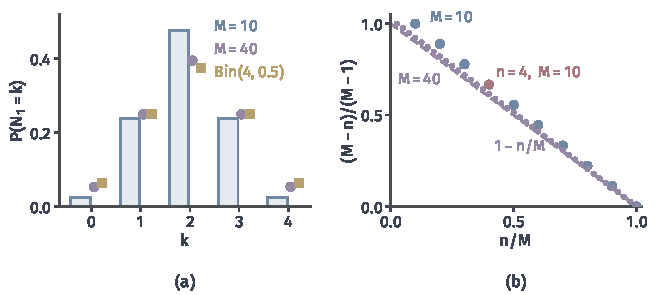
\includegraphics[width=112mm]{figures/07-probability/01-elementary-probability/matplotlib/mvd-hypergeom-approx/figure.pdf}
  \caption{不放回与放回抽样的比较，第$1$类比例$0.5$，抽取$n=4$个。(a)第$1$类计数$N_1$的质量函数：总体$M=10$（蓝色柱）、$M=40$（紫点）与$\operatorname{Bin}(4,0.5)$（黄色方块）。(b)方差因子$(M-n)/(M-1)$随抽样比例$n/M$的变化，蓝点为$M=10$，紫点为$M=40$，紫色虚线为$1-n/M$；红点是本节例子$n=4$、$M=10$。}
  \label{fig:mvd-hypergeom-approx}
\end{BookInlineFigure}

具体数值是：$M=10$时$\mathbb{P}(N_1=2)=100/210\approx0.476$，$M=40$时约为$0.395$，二项分布为$6/16=0.375$。抽样比例从$0.4$降到$0.1$，差距从$0.10$缩小到$0.02$。抽样比例不小时，应当保留有限总体的结构，否则会高估计数的波动，还会给超出$K_i$的计数分配概率。


\section{多元高斯分布}
\label{sec:mvd-gaussian}

两台传感器测量同一房间的温度，各自有测量误差。误差由许多小扰动叠加而成，其中有的扰动只影响一台传感器，比如各自电路的噪声；有的同时影响两台，比如房间里的气流。设三个扰动$Z_1,Z_2,Z_3$相互独立，都服从$\mathcal{N}(0,1)$，第一台读数受$Z_1,Z_2$影响，第二台受$Z_2,Z_3$影响：
\[
 X_1=2+Z_1+Z_2,\qquad X_2=1+Z_2+Z_3 .
\]
两个读数共享$Z_2$，所以一起偏高、一起偏低的机会更大。

这个例子已经包含了多元高斯分布的构造方式：从独立的标准高斯变量出发，做一次仿射变换。一元时，$\mathcal{N}(\mu,\sigma^{2})$就是$\mu+\sigma Z$的分布；多元时，把$\sigma$换成矩阵。本节先说明这样构造出的分布只由均值向量和协方差矩阵决定，再在两个小节中研究它的支撑与密度、条件分布与独立性。由样本估计$\bm{\mu}$与$\bm{\Sigma}$属于统计推断，归卷八处理。

\paragraph{标准高斯向量}
设$Z_1,\ldots,Z_k$相互独立，都服从$\mathcal{N}(0,1)$，记$\bm{Z}=(Z_1,\ldots,Z_k)^{\top}$，称为$k$维标准高斯向量，记为$\bm{Z}\sim\mathcal{N}(\bm{0},\bm{I}_k)$。独立变量的联合密度是边缘密度之积，
\[
 \varphi_k(\bm{z})=\prod_{i=1}^{k}\frac{1}{\sqrt{2\pi}}\mathrm{e}^{-z_i^{2}/2}=\frac{1}{(2\pi)^{k/2}}\mathrm{e}^{-\lVert\bm{z}\rVert_2^{2}/2} .
\]
这个密度只依赖$\bm{z}$到原点的距离，等密度线是同心球面。由此得到一个后面反复要用的事实：把标准高斯向量旋转一下，分布不变。

\begin{lemma}[旋转不变性]
\label{lem:mvd-rotation}
设$\bm{Z}\sim\mathcal{N}(\bm{0},\bm{I}_k)$。若$\bm{Q}$是$k\times k$正交矩阵，则$\bm{Q}\bm{Z}$与$\bm{Z}$同分布。若$r\times k$矩阵$\bm{C}$满足$\bm{C}\bm{C}^{\top}=\bm{I}_r$，则$\bm{C}\bm{Z}\sim\mathcal{N}(\bm{0},\bm{I}_r)$。
\end{lemma}

\begin{proof}
对$\mathbb{R}^{k}$中的区域$S$，事件$\bm{Q}\bm{Z}\in S$就是$\bm{Z}\in\bm{Q}^{\top}S$，所以
\[
 \mathbb{P}(\bm{Q}\bm{Z}\in S)=\int_{\bm{Q}^{\top}S}\varphi_k(\bm{z})\,\mathrm{d}\bm{z} .
\]
作线性换元$\bm{z}=\bm{Q}^{\top}\bm{x}$，积分区域变回$S$，Jacobian行列式的绝对值是$\lvert\det\bm{Q}^{\top}\rvert=1$（换元公式可参考\BookChapterRef{chap:region-integrals}{卷二第24章“区域积分”}）。又$\bm{Q}^{\top}$保持向量的长度，被积函数不变，于是
\[
 \mathbb{P}(\bm{Q}\bm{Z}\in S)=\int_{S}\varphi_k(\bm{x})\,\mathrm{d}\bm{x}=\mathbb{P}(\bm{Z}\in S) .
\]

对第二个结论，$\bm{C}$的$r$行是$\mathbb{R}^{k}$中的标准正交向量组，可以补成一组标准正交基，排成正交矩阵$\bm{Q}$，其前$r$行就是$\bm{C}$。由第一部分，$\bm{Q}\bm{Z}$是标准高斯向量，它的$k$个分量相互独立且都服从$\mathcal{N}(0,1)$。$\bm{C}\bm{Z}$是其中前$r$个分量，自然也是这样。
\end{proof}

\paragraph{仿射构造}
设$\bm{A}$是$d\times k$矩阵，$\bm{\mu}\in\mathbb{R}^{d}$，令$\bm{X}=\bm{\mu}+\bm{A}\bm{Z}$。由期望的线性性，$\mathbb{E}[\bm{X}]=\bm{\mu}$；由第~\ref{chap:random-vectors}章协方差矩阵的线性变换规则，
\[
 \operatorname{Cov}(\bm{X})=\bm{A}\operatorname{Cov}(\bm{Z})\bm{A}^{\top}=\bm{A}\bm{A}^{\top} .
\]
开头的传感器例子中，$\bm{\mu}=(2,1)^{\top}$，$k=3$，
\[
 \bm{A}=\begin{bmatrix}1&1&0\\0&1&1\end{bmatrix},\qquad
 \bm{A}\bm{A}^{\top}=\begin{bmatrix}2&1\\1&2\end{bmatrix} .
\]
非对角元$1$正是共享的$Z_2$贡献的方差。

同一个协方差矩阵可以由许多不同的$\bm{A}$得到。例如二阶方阵
\[
 \bm{L}=\begin{bmatrix}\sqrt2&0\\1/\sqrt2&\sqrt{3/2}\end{bmatrix}
\]
也满足$\bm{L}\bm{L}^{\top}=\bm{A}\bm{A}^{\top}$，它是Cholesky因子；对称平方根$\bm{\Sigma}^{1/2}$是另一个选择。用“三个扰动”还是“两个扰动”来生成，得到的读数分布会不会不同？下面的定理说不会：分布只认$\bm{\mu}$和$\bm{A}\bm{A}^{\top}$。

\begin{theorem}[多元高斯由均值与协方差确定]
\label{thm:mvd-gaussian-well-defined}
设$\bm{Z}\sim\mathcal{N}(\bm{0},\bm{I}_k)$，$\bm{Z}'\sim\mathcal{N}(\bm{0},\bm{I}_{k'})$，$\bm{A}$、$\bm{A}'$分别是$d\times k$与$d\times k'$矩阵。若$\bm{A}\bm{A}^{\top}=\bm{A}'\bm{A}'^{\top}$，则$\bm{\mu}+\bm{A}\bm{Z}$与$\bm{\mu}+\bm{A}'\bm{Z}'$同分布。并且每个$d\times d$对称半正定矩阵$\bm{\Sigma}$都能写成某个$\bm{A}\bm{A}^{\top}$。
\end{theorem}

\begin{proof}
记$\bm{\Sigma}=\bm{A}\bm{A}^{\top}$，秩为$r$。由谱分解（可参考\BookChapterRef{chap:eigen-spectral-decomposition}{卷二第6章“谱分解”}），
\[
 \bm{\Sigma}=\sum_{i=1}^{r}\lambda_i\bm{v}_i\bm{v}_i^{\top},\qquad \lambda_i>0,\ \bm{v}_i\text{标准正交} .
\]
令$\bm{B}$的第$i$列为$\sqrt{\lambda_i}\bm{v}_i$，则$\bm{B}$是$d\times r$矩阵，列满秩，$\bm{B}\bm{B}^{\top}=\bm{\Sigma}$。我们证明$\bm{A}\bm{Z}$与$\bm{B}\bm{W}$同分布，其中$\bm{W}\sim\mathcal{N}(\bm{0},\bm{I}_r)$；$\bm{A}'$同理，两者便同分布。

第一步，$\bm{A}$与$\bm{\Sigma}$的列空间相同。由$\bm{\Sigma}\bm{y}=\bm{A}(\bm{A}^{\top}\bm{y})$，$\bm{\Sigma}$的列空间含于$\bm{A}$的列空间。反过来，若$\bm{v}$与$\bm{\Sigma}$的列空间正交，则$\bm{\Sigma}\bm{v}=\bm{0}$，于是
\[
 \lVert\bm{A}^{\top}\bm{v}\rVert_2^{2}=\bm{v}^{\top}\bm{\Sigma}\bm{v}=0 ,
\]
$\bm{v}$也与$\bm{A}$的列正交。两个列空间的正交补相同，所以列空间相同，也都等于$\bm{B}$的列空间。

第二步，把$\bm{A}$写成$\bm{B}\bm{C}$。$\bm{B}$列满秩，$\bm{B}^{\top}\bm{B}$可逆，令
\[
 \bm{B}^{+}=(\bm{B}^{\top}\bm{B})^{-1}\bm{B}^{\top} ,
\]
则$\bm{B}^{+}\bm{B}=\bm{I}_r$，而$\bm{B}\bm{B}^{+}$是到$\bm{B}$列空间的正交投影。$\bm{A}$的列都在这个空间里，所以
\[
 \bm{A}=\bm{B}\bm{B}^{+}\bm{A}=\bm{B}\bm{C},\qquad \bm{C}=\bm{B}^{+}\bm{A} .
\]

第三步，$\bm{C}$的行标准正交。直接计算，
\[
 \bm{C}\bm{C}^{\top}=\bm{B}^{+}\bm{A}\bm{A}^{\top}(\bm{B}^{+})^{\top}=\bm{B}^{+}\bm{B}\bm{B}^{\top}(\bm{B}^{+})^{\top}=\bm{I}_r .
\]
由引理~\ref{lem:mvd-rotation}，$\bm{C}\bm{Z}\sim\mathcal{N}(\bm{0},\bm{I}_r)$，于是$\bm{A}\bm{Z}=\bm{B}(\bm{C}\bm{Z})$与$\bm{B}\bm{W}$同分布。

最后，半正定矩阵$\bm{\Sigma}$的谱分解中$\lambda_i\geq0$，上面构造的$\bm{B}$就满足$\bm{B}\bm{B}^{\top}=\bm{\Sigma}$。
\end{proof}

证明的想法是：不同的$\bm{A}$只相差一次“旋转”，而标准高斯向量对旋转不敏感。传感器例子中，三个扰动经过$\bm{C}$压成两个独立的标准高斯变量，信息上没有丢失任何影响读数的东西。有了这个定理，下面的定义才有意义。

\begin{definition}[多元高斯分布]
\label{def:mvd-gaussian}
设$\bm{\mu}\in\mathbb{R}^{d}$，$\bm{\Sigma}$是$d\times d$对称半正定矩阵。若随机向量$\bm{X}$与$\bm{\mu}+\bm{A}\bm{Z}$同分布，其中$\bm{Z}\sim\mathcal{N}(\bm{0},\bm{I}_k)$，$\bm{A}$为满足
\begin{equation}
 \bm{A}\bm{A}^{\top}=\bm{\Sigma}
 \label{eq:mvd-gaussian-factor}
\end{equation}
的$d\times k$矩阵，则称$\bm{X}$服从均值为$\bm{\mu}$、协方差矩阵为$\bm{\Sigma}$的\term{多元高斯分布}（multivariate Gaussian distribution），记为$\bm{X}\sim\mathcal{N}(\bm{\mu},\bm{\Sigma})$，也说$\bm{X}$的分量\term{联合高斯}（jointly Gaussian）。
\end{definition}

这里$\bm{\Sigma}$是粗体大写的矩阵，与求和号无关。传感器例子中$\bm{X}\sim\mathcal{N}(\bm{\mu},\bm{\Sigma})$，$\bm{\mu}=(2,1)^{\top}$，$\bm{\Sigma}$的对角元为$2$、非对角元为$1$，本节一直用这组参数。图~\ref{fig:mvd-gauss-affine}把$400$个标准高斯点经过$\bm{x}=\bm{\mu}+\bm{\Sigma}^{1/2}\bm{z}$映过去：圆被拉成斜放的椭圆，点云随之倾斜。

\begin{BookInlineFigure}
  \centering
  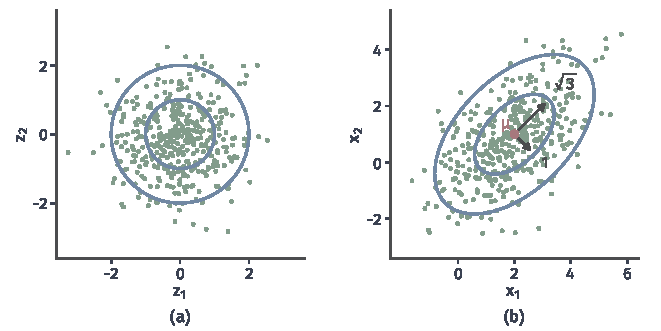
\includegraphics[width=112mm]{figures/07-probability/01-elementary-probability/matplotlib/mvd-gauss-affine/figure.pdf}
  \caption{仿射构造。(a)$400$个二维标准高斯点（绿，种子$7$）与半径$1$、$2$的圆（蓝）。(b)同一批点经$\bm{x}=\bm{\mu}+\bm{\Sigma}^{1/2}\bm{z}$映射后的位置，$\bm{\mu}=(2,1)^{\top}$（红点），$\Sigma_{1,1}=\Sigma_{2,2}=2$，$\Sigma_{1,2}=1$；圆变成椭圆，箭头是两条主轴方向，半轴长分别为$\sqrt3$与$1$。}
  \label{fig:mvd-gauss-affine}
\end{BookInlineFigure}

\paragraph{仿射变换与边缘分布}
构造方式本身就是仿射变换，所以再做一次仿射变换，结果仍是多元高斯。设$\bm{X}\sim\mathcal{N}(\bm{\mu},\bm{\Sigma})$，$\bm{M}$是$m\times d$矩阵，$\bm{c}\in\mathbb{R}^{m}$。把$\bm{X}$写成$\bm{\mu}+\bm{A}\bm{Z}$，
\[
 \bm{M}\bm{X}+\bm{c}=(\bm{M}\bm{\mu}+\bm{c})+(\bm{M}\bm{A})\bm{Z},\qquad (\bm{M}\bm{A})(\bm{M}\bm{A})^{\top}=\bm{M}\bm{\Sigma}\bm{M}^{\top} .
\]由定义~\ref{def:mvd-gaussian}，
\begin{equation}
 \bm{M}\bm{X}+\bm{c}\sim\mathcal{N}\bigl(\bm{M}\bm{\mu}+\bm{c},\ \bm{M}\bm{\Sigma}\bm{M}^{\top}\bigr) .
 \label{eq:mvd-gaussian-affine}
\end{equation}
这里不要求$\bm{M}$满秩，也不要求$m\leq d$。

两种特殊的$\bm{M}$最常用。取$\bm{M}$为单位矩阵的若干行，$\bm{M}\bm{X}$就是$\bm{X}$的一部分分量，于是边缘分布不必积分，只要从$\bm{\mu}$和$\bm{\Sigma}$中取出对应的子向量和子矩阵。取$\bm{M}=\bm{a}^{\top}$，得到一元线性组合
\[
 \bm{a}^{\top}\bm{X}\sim\mathcal{N}(\bm{a}^{\top}\bm{\mu},\ \bm{a}^{\top}\bm{\Sigma}\bm{a}) .
\]
方差为$0$时，$\mathcal{N}(m,0)$理解为恒取$m$的退化分布。

传感器例子中，$X_1\sim\mathcal{N}(2,2)$，$X_2\sim\mathcal{N}(1,2)$。两台读数之和与之差分别是
\[
 \begin{aligned}
  X_1+X_2&\sim\mathcal{N}(3,\,2+2+2\times1)=\mathcal{N}(3,6),\\
  X_1-X_2&\sim\mathcal{N}(1,\,2+2-2\times1)=\mathcal{N}(1,2) .
 \end{aligned}
\]
共享的扰动在和里叠加，在差里抵消，所以差的方差比和小。

\subsection{协方差与支撑}
\label{sec:mvd-gaussian-support}

定义~\ref{def:mvd-gaussian}只要求$\bm{\Sigma}$半正定。$\bm{\Sigma}$正定时，分布铺满整个$\mathbb{R}^{d}$，有普通的$d$维密度；$\bm{\Sigma}$奇异时，分布挤在一个低维的平面里。下面分别看这两种情形，再说明怎样判断一个随机向量是不是联合高斯。

\paragraph{正定协方差与密度}
$\bm{\Sigma}$正定时可以取方阵$\bm{A}$。例如Cholesky分解$\bm{\Sigma}=\bm{L}\bm{L}^{\top}$给出可逆的下三角矩阵$\bm{L}$（可参考\BookChapterRef{chap:direct-linear-solvers}{卷二第12章“线性方程的直接求解”}）。于是$\bm{X}=\bm{\mu}+\bm{L}\bm{Z}$是对标准高斯向量做可逆仿射变换，可以把$\bm{Z}$的密度搬过来。

\begin{theorem}[多元高斯密度]
\label{thm:mvd-gaussian-density}
设$\bm{\Sigma}$正定，$\bm{X}\sim\mathcal{N}(\bm{\mu},\bm{\Sigma})$，则$\bm{X}$有联合密度
\begin{equation}
 f_{\bm{X}}(\bm{x})=\frac{1}{(2\pi)^{d/2}(\det\bm{\Sigma})^{1/2}}\exp\Bigl(-\frac12Q(\bm{x})\Bigr),\qquad \bm{x}\in\mathbb{R}^{d},
 \label{eq:mvd-gaussian-density}
\end{equation}
其中
\begin{equation}
 Q(\bm{x})=(\bm{x}-\bm{\mu})^{\top}\bm{\Sigma}^{-1}(\bm{x}-\bm{\mu}) .
 \label{eq:mvd-gaussian-quadratic}
\end{equation}
\end{theorem}

\begin{proof}
对区域$S$，事件$\bm{X}\in S$就是$\bm{Z}\in\bm{L}^{-1}(S-\bm{\mu})$，所以
\[
 \mathbb{P}(\bm{X}\in S)=\int_{\bm{L}^{-1}(S-\bm{\mu})}\varphi_d(\bm{z})\,\mathrm{d}\bm{z} .
\]
作线性换元$\bm{z}=\bm{L}^{-1}(\bm{x}-\bm{\mu})$，积分区域变成$S$，体积元变为$\lvert\det\bm{L}^{-1}\rvert\,\mathrm{d}\bm{x}$。由$\det\bm{\Sigma}=(\det\bm{L})^{2}$，
\[
 \lvert\det\bm{L}^{-1}\rvert=(\det\bm{\Sigma})^{-1/2} .
\]
又$\bm{L}^{-\top}\bm{L}^{-1}=\bm{\Sigma}^{-1}$，所以$\lVert\bm{z}\rVert_2^{2}=Q(\bm{x})$。代入即得：$\bm{X}$落在$S$中的概率等于$f_{\bm{X}}$在$S$上的积分。
\end{proof}

公式的两部分各有来历。指数里的$Q(\bm{x})$是把偏离量$\bm{x}-\bm{\mu}$“还原”成标准高斯坐标后的平方长度；前面的$(\det\bm{\Sigma})^{-1/2}$是体积的缩放：$\bm{L}$把单位体积拉成$\det\bm{L}$倍，同样多的概率摊在更大的体积上，密度就按同一倍数降低。$d=1$时$Q=(x-\mu)^{2}/\sigma^{2}$，回到一元高斯密度。证明中的线性换元在第~\ref{chap:random-variable-transformations}章发展为一般的密度换元公式。

传感器例子中，$\det\bm{\Sigma}=3$，
\[
 \bm{\Sigma}^{-1}=\frac13\begin{bmatrix}2&-1\\-1&2\end{bmatrix} .
\]
记$u_1=x_1-2$，$u_2=x_2-1$，则$Q=\tfrac23(u_1^{2}-u_1u_2+u_2^{2})$，密度为
\[
 f_{\bm{X}}(\bm{x})=\frac{1}{2\sqrt3\,\pi}\exp\Bigl(-\frac{u_1^{2}-u_1u_2+u_2^{2}}{3}\Bigr) .
\]
在$\bm{x}=\bm{\mu}$处取最大值$1/(2\sqrt3\,\pi)\approx0.0919$。

\paragraph{等密度椭球与马氏距离}
密度只通过$Q(\bm{x})$依赖$\bm{x}$，等密度集是$Q(\bm{x})=c^{2}$。用谱分解
\[
 \bm{\Sigma}=\sum_{i=1}^{d}\lambda_i\bm{v}_i\bm{v}_i^{\top},\qquad \bm{\Sigma}^{-1}=\sum_{i=1}^{d}\lambda_i^{-1}\bm{v}_i\bm{v}_i^{\top},
\]
在以$\bm{\mu}$为原点、以$\bm{v}_i$为坐标轴的坐标$y_i=\bm{v}_i^{\top}(\bm{x}-\bm{\mu})$下，
\[
 Q(\bm{x})=\sum_{i=1}^{d}\frac{y_i^{2}}{\lambda_i} .
\]
所以$Q=c^{2}$是以$\bm{\mu}$为中心的椭球，主轴沿特征向量$\bm{v}_i$，半轴长为$c\sqrt{\lambda_i}$。方差大的方向椭球长，方差小的方向椭球扁。

量$\sqrt{Q(\bm{x})}$称为$\bm{x}$到$\bm{\mu}$的\term{马氏距离}（Mahalanobis distance）。它按各方向的波动大小度量偏离：沿方差大的方向走一段距离，算作较小的偏离。传感器例子的特征值是$3$和$1$，对应方向$(1,1)^{\top}/\sqrt2$与$(1,-1)^{\top}/\sqrt2$。两台读数同向偏离较常见，反向偏离较少见。

取两点$\bm{a}=\bm{\mu}+(1,1)^{\top}$和$\bm{b}=\bm{\mu}+(1,-1)^{\top}$，它们到$\bm{\mu}$的欧氏距离都是$\sqrt2$。代入$Q$，
\[
 Q(\bm{a})=\tfrac23(1-1+1)=\tfrac23,\qquad Q(\bm{b})=\tfrac23(1+1+1)=2 .
\]
两者相差$4/3$，密度之比为$\mathrm{e}^{2/3}\approx1.95$。图~\ref{fig:mvd-gauss-mahalanobis}(a)中，$\bm{a}$落在较内的椭圆上，$\bm{b}$落在较外的椭圆上，尽管两者在同一个欧氏圆上。

\begin{BookInlineFigure}
  \centering
  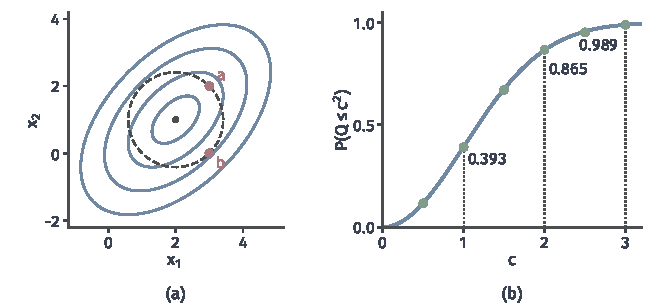
\includegraphics[width=112mm]{figures/07-probability/01-elementary-probability/matplotlib/mvd-gauss-mahalanobis/figure.pdf}
  \caption{马氏距离与椭圆概率。(a)传感器例子的等密度椭圆$Q=c^{2}$，$c=0.5,1,1.5,2$（蓝）；虚线圆是到$\bm{\mu}$（深灰点）欧氏距离为$\sqrt2$的点，红点$a$、$b$在圆上，马氏距离分别为$\sqrt{2/3}$与$\sqrt2$。(b)二维情形椭圆内的概率$1-\mathrm{e}^{-c^{2}/2}$（蓝），绿点是$4000$个模拟点（种子$11$）落入椭圆的比例。}
  \label{fig:mvd-gauss-mahalanobis}
\end{BookInlineFigure}

椭圆内的概率也可以直接算。$\bm{X}=\bm{\mu}+\bm{L}\bm{Z}$时，证明中已经看到$Q(\bm{X})=\lVert\bm{Z}\rVert_2^{2}$，所以$\mathbb{P}(Q(\bm{X})\leq c^{2})$与$\bm{\mu}$、$\bm{\Sigma}$都无关。$d=2$时用极坐标计算，
\[
 \mathbb{P}\bigl(\lVert\bm{Z}\rVert_2\leq c\bigr)=\int_0^{2\pi}\!\!\int_0^{c}\frac{1}{2\pi}\mathrm{e}^{-r^{2}/2}\,r\,\mathrm{d}r\,\mathrm{d}\theta=1-\mathrm{e}^{-c^{2}/2} .
\]
$c=1,2,3$时分别约为$0.393$、$0.865$、$0.989$。一元时均值加减一个标准差内有约$68\%$的概率，二维的“一个马氏距离”椭圆内只有约$39\%$：维数越高，概率越往外层分布。一般维数下$\lVert\bm{Z}\rVert_2^{2}$服从$\chi^2_d$分布，这在第~\ref{chap:random-variable-transformations}章说明。

\paragraph{奇异协方差与低维支撑}
现在设$\bm{\Sigma}$的秩$r<d$。定理~\ref{thm:mvd-gaussian-well-defined}的证明给出$\bm{X}$与$\bm{\mu}+\bm{B}\bm{W}$同分布，其中$\bm{B}$是$d\times r$矩阵，其列空间就是$\bm{\Sigma}$的列空间。$\bm{B}\bm{W}$总在这个列空间里，所以$\bm{X}$以概率$1$落在仿射子空间
\[
 \bm{\mu}+\{\bm{\Sigma}\bm{y}:\bm{y}\in\mathbb{R}^{d}\},
\]
其维数为$r$。这样的分布称为\term{退化高斯分布}（degenerate Gaussian distribution）。

退化的分布没有$d$维密度。$r<d$维的仿射子空间的$d$维体积为$0$，任何$d$维密度在它上面的积分都是$0$，不可能给它概率$1$。不过在子空间内部换用$r$个坐标$\bm{W}$，分布又是非退化的。

还可以从另一面看这件事。若$\bm{\Sigma}\bm{v}=\bm{0}$，则$\bm{v}^{\top}\bm{X}$的方差$\bm{v}^{\top}\bm{\Sigma}\bm{v}$为$0$，由式~\eqref{eq:mvd-gaussian-affine}，$\bm{v}^{\top}\bm{X}$服从$\mathcal{N}(\bm{v}^{\top}\bm{\mu},0)$，恒等于常数。零空间中的每个方向都对应$\bm{X}$满足的一条线性约束，$d-r$条约束把分布压进$r$维平面。

传感器例子中，令$S=X_1+X_2$，再记录$\bm{Y}=(S,2S)^{\top}$。取$\bm{M}$的两行分别为$(1,1)$和$(2,2)$，由式~\eqref{eq:mvd-gaussian-affine}，
\[
 \bm{Y}\sim\mathcal{N}\Biggl(\begin{bmatrix}3\\6\end{bmatrix},\ 6\begin{bmatrix}1&2\\2&4\end{bmatrix}\Biggr) .
\]
协方差矩阵的秩为$1$，零空间由$\bm{v}=(2,-1)^{\top}$张成，对应约束$2Y_1-Y_2=0$。图~\ref{fig:mvd-gauss-degenerate}(a)中所有样本点都在直线$y_2=2y_1$上；沿直线的坐标$S\sim\mathcal{N}(3,6)$有普通的一元密度，图~\ref{fig:mvd-gauss-degenerate}(b)。

\begin{BookInlineFigure}
  \centering
  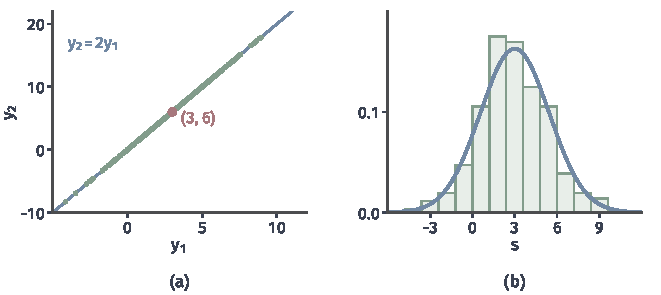
\includegraphics[width=112mm]{figures/07-probability/01-elementary-probability/matplotlib/mvd-gauss-degenerate/figure.pdf}
  \caption{退化高斯分布。(a)$\bm{Y}=(S,2S)^{\top}$的$300$个样本（绿，种子$5$），$S=X_1+X_2$；全部落在直线$y_2=2y_1$（蓝）上，红点为均值$(3,6)$。(b)沿直线的坐标$S$的直方图（浅绿）与$\mathcal{N}(3,6)$密度（蓝）。}
  \label{fig:mvd-gauss-degenerate}
\end{BookInlineFigure}

\paragraph{怎样判断联合高斯}
由式~\eqref{eq:mvd-gaussian-affine}，联合高斯向量的每个分量、每个线性组合$\bm{a}^{\top}\bm{X}$都服从一元高斯分布（方差可能为$0$）。反过来也成立：若对每个$\bm{a}\in\mathbb{R}^{d}$，$\bm{a}^{\top}\bm{X}$都服从一元高斯分布，则$\bm{X}$联合高斯。这个方向本章不证，证明要用到“特征函数唯一确定分布”，特征函数在第~\ref{chap:weak-convergence-of-distributions}章建立。它说明联合高斯是关于所有方向的条件，不是只关于坐标方向的条件。

只检查坐标方向是不够的。设$Z\sim\mathcal{N}(0,1)$，$S$以各$1/2$的概率取$\pm1$，与$Z$独立，考虑$(Z,SZ)$。第二个分量也服从$\mathcal{N}(0,1)$：
\[
 \mathbb{P}(SZ\leq t)=\tfrac12\mathbb{P}(Z\leq t)+\tfrac12\mathbb{P}(-Z\leq t)=\mathbb{P}(Z\leq t) ,
\]
这里用了$-Z$与$Z$同分布。两个分量都是标准高斯。

可是线性组合$Z+SZ$在$S=-1$时恒为$0$，所以$\mathbb{P}(Z+SZ=0)=1/2$。方差为正的一元高斯分布在单点上的概率为$0$，方差为$0$的又只取一个值，$Z+SZ$两样都不是，因而$(Z,SZ)$不是联合高斯。图~\ref{fig:mvd-random-sign}(a)中它的样本只落在两条对角线上，(b)中和的分布有一个质量为$1/2$的原子。

\begin{BookInlineFigure}
  \centering
  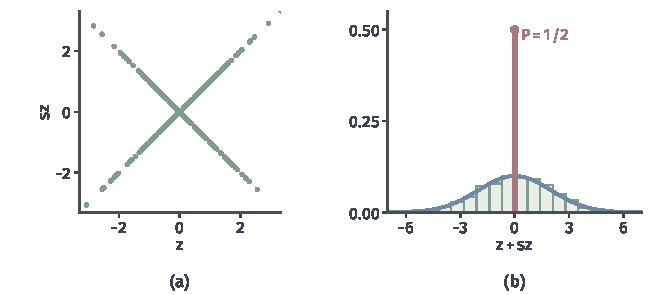
\includegraphics[width=112mm]{figures/07-probability/01-elementary-probability/matplotlib/mvd-random-sign/figure.pdf}
  \caption{分量各自高斯但不联合高斯。(a)$(Z,SZ)$的$400$个样本（绿，种子$3$），$S=\pm1$等可能且与$Z$独立；点只落在两条对角线上。(b)$Z+SZ$的分布：$0$处有概率$1/2$的原子（红），其余部分的密度为$\tfrac12$倍$\mathcal{N}(0,4)$密度（蓝），绿色直方图来自$4000$个模拟值。}
  \label{fig:mvd-random-sign}
\end{BookInlineFigure}

\subsection{条件分布与正交分解}
\label{sec:mvd-gaussian-conditional}

观测到第一台传感器的读数以后，第二台读数的分布变成什么？更一般地，把$\bm{X}$的分量分成两组，观测其中一组，另一组的条件分布是什么？两组什么时候相互独立？为此把$\bm{X}$与参数按相同方式分块：
\[
 \bm{X}=\begin{bmatrix}\bm{X}_a\\\bm{X}_b\end{bmatrix},\qquad
 \bm{\mu}=\begin{bmatrix}\bm{\mu}_a\\\bm{\mu}_b\end{bmatrix},\qquad
 \bm{\Sigma}=\begin{bmatrix}\bm{\Sigma}_{aa}&\bm{\Sigma}_{ab}\\\bm{\Sigma}_{ba}&\bm{\Sigma}_{bb}\end{bmatrix} ,
\]
其中交叉协方差$\bm{\Sigma}_{ab}$就是$\operatorname{Cov}(\bm{X}_a,\bm{X}_b)$，且$\bm{\Sigma}_{ba}=\bm{\Sigma}_{ab}^{\top}$。两组的边缘分布只用到对角块，两组之间的联系全部记在$\bm{\Sigma}_{ab}$里。

\paragraph{零交叉协方差推出独立}
第~\ref{chap:random-vectors}章说明，独立推出不相关，反过来一般不成立。联合高斯是一个重要的例外。

\begin{theorem}[联合高斯的分块独立]
\label{thm:mvd-gaussian-independence}
设$\bm{X}\sim\mathcal{N}(\bm{\mu},\bm{\Sigma})$按上述方式分块。若$\bm{\Sigma}_{ab}=\bm{0}$，则$\bm{X}_a$与$\bm{X}_b$相互独立。
\end{theorem}

\begin{proof}
取矩阵$\bm{A}_a$、$\bm{A}_b$使$\bm{A}_a\bm{A}_a^{\top}=\bm{\Sigma}_{aa}$，$\bm{A}_b\bm{A}_b^{\top}=\bm{\Sigma}_{bb}$，列数分别为$k_a$、$k_b$，再令
\[
 \bm{A}=\begin{bmatrix}\bm{A}_a&\bm{0}\\\bm{0}&\bm{A}_b\end{bmatrix} .
\]
因为$\bm{\Sigma}_{ab}=\bm{0}$，有$\bm{A}\bm{A}^{\top}=\bm{\Sigma}$。由定理~\ref{thm:mvd-gaussian-well-defined}，$\bm{X}$与$\bm{\mu}+\bm{A}\bm{Z}$同分布。把$\bm{Z}$分成前$k_a$个分量$\bm{Z}'$与后$k_b$个分量$\bm{Z}''$，就有
\[
 \bm{X}_a\overset{\mathrm{d}}{=}\bm{\mu}_a+\bm{A}_a\bm{Z}',\qquad \bm{X}_b\overset{\mathrm{d}}{=}\bm{\mu}_b+\bm{A}_b\bm{Z}'' ,
\]
这里$\overset{\mathrm{d}}{=}$表示两组同时同分布。

$\bm{Z}'$与$\bm{Z}''$由不同的独立分量组成，联合密度是两部分密度之积，因而相互独立。对区域$S$、$T$，记$S'$、$T''$为它们在两个仿射映射下的原像，于是
\[
 \mathbb{P}(\bm{X}_a\in S,\ \bm{X}_b\in T)=\mathbb{P}(\bm{Z}'\in S',\ \bm{Z}''\in T'')=\mathbb{P}(\bm{Z}'\in S')\,\mathbb{P}(\bm{Z}''\in T'') .
\]
右边两个因子分别是$\mathbb{P}(\bm{X}_a\in S)$与$\mathbb{P}(\bm{X}_b\in T)$。
\end{proof}

证明没有用到密度，所以$\bm{\Sigma}$奇异时同样成立。逐个分量应用：联合高斯向量的协方差矩阵若是对角的，各分量相互独立。

定理的前提是整个向量联合高斯。上一小节的$(Z,SZ)$中，
\[
 \operatorname{Cov}(Z,SZ)=\mathbb{E}[S]\,\mathbb{E}[Z^{2}]=0 ,
\]
两个分量不相关，也都是标准高斯，却不独立：$\lvert SZ\rvert=\lvert Z\rvert$，知道$Z$以后，$SZ$只剩$\pm Z$两种可能。定理不适用，正是因为它们不联合高斯。

\paragraph{配方求条件分布}
设$\bm{\Sigma}$正定，于是对角块$\bm{\Sigma}_{bb}$也正定，可逆。目标是把联合密度写成“$\bm{x}_b$的边缘密度”乘以“$\bm{x}_a$的某个高斯密度”。关键是对二次型$Q$关于$\bm{x}_a$配方，用矩阵语言就是一步分块消元。令
\[
 \bm{K}=\bm{\Sigma}_{ab}\bm{\Sigma}_{bb}^{-1},\qquad
 \bm{S}=\bm{\Sigma}_{aa}-\bm{\Sigma}_{ab}\bm{\Sigma}_{bb}^{-1}\bm{\Sigma}_{ba},\qquad
 \bm{E}=\begin{bmatrix}\bm{I}&-\bm{K}\\\bm{0}&\bm{I}\end{bmatrix} .
\]
$\bm{S}$是$\bm{\Sigma}$中块$\bm{\Sigma}_{bb}$的Schur补（可参考\BookChapterRef{chap:direct-linear-solvers}{卷二第12章“线性方程的直接求解”}）。

先左乘$\bm{E}$。第一块行的第二块变为$\bm{\Sigma}_{ab}-\bm{K}\bm{\Sigma}_{bb}=\bm{0}$，
\[
 \bm{E}\bm{\Sigma}=\begin{bmatrix}\bm{S}&\bm{0}\\\bm{\Sigma}_{ba}&\bm{\Sigma}_{bb}\end{bmatrix} .
\]
再右乘$\bm{E}^{\top}$。第二块行的第一块变为$\bm{\Sigma}_{ba}-\bm{\Sigma}_{bb}\bm{K}^{\top}$，由$\bm{\Sigma}_{bb}\bm{K}^{\top}=\bm{\Sigma}_{ba}$，它也是$\bm{0}$，得到
\begin{equation}
 \bm{E}\bm{\Sigma}\bm{E}^{\top}=\begin{bmatrix}\bm{S}&\bm{0}\\\bm{0}&\bm{\Sigma}_{bb}\end{bmatrix} .
 \label{eq:mvd-block-elimination}
\end{equation}

式~\eqref{eq:mvd-block-elimination}给出三件事。$\bm{E}$可逆，所以右边与$\bm{\Sigma}$同为正定，$\bm{S}$正定。$\det\bm{E}=1$，所以行列式按块分解。两边求逆，又得到$\bm{\Sigma}^{-1}$的分解：
\[
 \det\bm{\Sigma}=\det\bm{S}\cdot\det\bm{\Sigma}_{bb},\qquad
 \bm{\Sigma}^{-1}=\bm{E}^{\top}\begin{bmatrix}\bm{S}^{-1}&\bm{0}\\\bm{0}&\bm{\Sigma}_{bb}^{-1}\end{bmatrix}\bm{E} .
\]

把最后一式代入$Q$。记$\bm{u}=\bm{x}-\bm{\mu}$，则$\bm{E}\bm{u}$的两块是$\bm{u}_a-\bm{K}\bm{u}_b$与$\bm{u}_b$，于是
\[
 Q(\bm{x})=(\bm{u}_a-\bm{K}\bm{u}_b)^{\top}\bm{S}^{-1}(\bm{u}_a-\bm{K}\bm{u}_b)+\bm{u}_b^{\top}\bm{\Sigma}_{bb}^{-1}\bm{u}_b .
\]
这就是配方的结果：第一项是$\bm{x}_a$围绕$\bm{\mu}_a+\bm{K}\bm{u}_b$的二次型，第二项只含$\bm{x}_b$。

把配方结果和行列式的分解代入式~\eqref{eq:mvd-gaussian-density}，常数与指数都按两组拆开，联合密度成为两个高斯密度之积：第一个是$\bm{x}_a$的均值为$\bm{\mu}_a+\bm{K}\bm{u}_b$、协方差为$\bm{S}$的密度，第二个是$\mathcal{N}(\bm{\mu}_b,\bm{\Sigma}_{bb})$的密度。后者正是$\bm{X}_b$的边缘密度。除以它，按第~\ref{chap:random-vectors}章条件密度的定义得到下面的定理。

\begin{theorem}[高斯条件分布]
\label{thm:mvd-gaussian-conditional}
设$\bm{\Sigma}$正定，$\bm{X}\sim\mathcal{N}(\bm{\mu},\bm{\Sigma})$按上述方式分块。对每个$\bm{x}_b$，给定$\bm{X}_b=\bm{x}_b$时$\bm{X}_a$的条件分布是高斯分布，条件均值与条件协方差分别为
\begin{align}
 \mathbb{E}[\bm{X}_a\mid\bm{X}_b=\bm{x}_b]&=\bm{\mu}_a+\bm{\Sigma}_{ab}\bm{\Sigma}_{bb}^{-1}(\bm{x}_b-\bm{\mu}_b),
 \label{eq:mvd-gauss-cond-mean}\\
 \operatorname{Cov}(\bm{X}_a\mid\bm{X}_b=\bm{x}_b)&=\bm{\Sigma}_{aa}-\bm{\Sigma}_{ab}\bm{\Sigma}_{bb}^{-1}\bm{\Sigma}_{ba} .
 \label{eq:mvd-gauss-cond-cov}
\end{align}
\end{theorem}

回到传感器，观测第一台读数$X_1=x_1$，求第二台$X_2$的条件分布。此时$\bm{X}_a=X_2$，$\bm{X}_b=X_1$，各块都是数：$\Sigma_{aa}=\Sigma_{bb}=2$，$\Sigma_{ab}=1$。代入式~\eqref{eq:mvd-gauss-cond-mean}和式~\eqref{eq:mvd-gauss-cond-cov}，
\[
 \mathbb{E}[X_2\mid X_1=x_1]=1+\frac{x_1-2}{2},\qquad \operatorname{Var}(X_2\mid X_1=x_1)=2-\frac{1}{2}=\frac32 .
\]

若第一台读到$x_1=4$，比均值高$2$，则$X_2\mid X_1=4\sim\mathcal{N}(2,3/2)$。观测之前$X_2\sim\mathcal{N}(1,2)$，$\mathbb{P}(X_2>2)=1-\Phi(1/\sqrt2)\approx0.240$，其中$\Phi$是标准高斯分布函数；观测之后，$\mathbb{P}(X_2>2\mid X_1=4)=0.5$。第一台偏高，把对第二台的预测中心从$1$推到$2$，方差从$2$缩到$1.5$。

图~\ref{fig:mvd-gauss-conditional}(a)中，竖直红线$x_1=4$切过等密度椭圆，切片上的密度重新归一化，就是条件密度；黄线是条件均值$m(x_1)=1+(x_1-2)/2$，它穿过每条竖直切片上密度最高的点。(b)比较了观测前后$X_2$的密度。

\begin{BookInlineFigure}
  \centering
  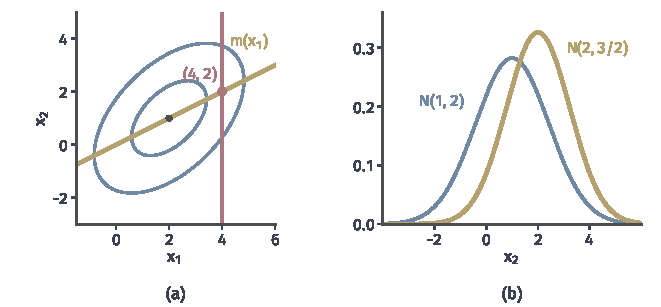
\includegraphics[width=112mm]{figures/07-probability/01-elementary-probability/matplotlib/mvd-gauss-conditional/figure.pdf}
  \caption{传感器例子的条件化。(a)等密度椭圆$Q=1,4$（蓝），观测$x_1=4$（红线），条件均值直线$m(x_1)=1+(x_1-2)/2$（黄），红点$(4,2)$是给定$X_1=4$时$X_2$的条件均值。(b)$X_2$的边缘密度$\mathcal{N}(1,2)$（蓝）与给定$X_1=4$后的条件密度$\mathcal{N}(2,3/2)$（黄）。}
  \label{fig:mvd-gauss-conditional}
\end{BookInlineFigure}

式~\eqref{eq:mvd-gauss-cond-mean}与式~\eqref{eq:mvd-gauss-cond-cov}有两个特点。条件均值是观测值的仿射函数，图中是一条直线。条件协方差完全不依赖观测值：无论第一台读到多少，第二台的剩余不确定性都是$1.5$。一般的联合分布中，条件方差会随条件取值变化，例如三角形区域上的均匀分布，固定的坐标越靠近顶点，另一个坐标可取的范围越窄，条件方差越小。不随观测值变化是高斯模型的特殊性质。

此外，$\bm{\Sigma}_{aa}$与$\bm{S}$之差是半正定矩阵$\bm{\Sigma}_{ab}\bm{\Sigma}_{bb}^{-1}\bm{\Sigma}_{ba}$，所以观测只会减少每个方向上的方差，不会增加。$\bm{\Sigma}_{ab}=\bm{0}$时$\bm{S}=\bm{\Sigma}_{aa}$，条件分布等于边缘分布，与定理~\ref{thm:mvd-gaussian-independence}一致。

\paragraph{正交分解}
条件协方差为什么不随观测值变化？把$\bm{X}_a$减去它的条件均值，看剩下的残差
\[
 \bm{R}=\bm{X}_a-\bm{\mu}_a-\bm{K}(\bm{X}_b-\bm{\mu}_b) .
\]
$(\bm{R},\bm{X}_b)$是$\bm{X}$的仿射像，由式~\eqref{eq:mvd-gaussian-affine}联合高斯。它们的交叉协方差是
\[
 \operatorname{Cov}(\bm{R},\bm{X}_b)=\bm{\Sigma}_{ab}-\bm{K}\bm{\Sigma}_{bb}=\bm{0} .
\]
由定理~\ref{thm:mvd-gaussian-independence}，$\bm{R}$与$\bm{X}_b$独立。

再算残差的协方差。展开后有三项交叉项，每一项都等于$\bm{\Sigma}_{ab}\bm{\Sigma}_{bb}^{-1}\bm{\Sigma}_{ba}$，于是
\[
 \operatorname{Cov}(\bm{R})=\bm{\Sigma}_{aa}-\bm{K}\bm{\Sigma}_{ba}-\bm{\Sigma}_{ab}\bm{K}^{\top}+\bm{K}\bm{\Sigma}_{bb}\bm{K}^{\top}=\bm{S} .
\]
所以$\bm{X}_a$分解成两部分：
\begin{equation}
 \bm{X}_a=\underbrace{\bm{\mu}_a+\bm{K}(\bm{X}_b-\bm{\mu}_b)}_{\text{由}\bm{X}_b\text{决定}}+\underbrace{\bm{R}}_{\text{与}\bm{X}_b\text{独立}},\qquad \bm{R}\sim\mathcal{N}(\bm{0},\bm{S}) .
 \label{eq:mvd-orthogonal-decomposition}
\end{equation}

观测$\bm{X}_b=\bm{x}_b$只确定了第一部分，残差的分布不受影响，所以条件分布是把$\mathcal{N}(\bm{0},\bm{S})$平移到条件均值处。$\bm{K}$的选择恰好使残差与$\bm{X}_b$不相关；用协方差作内积，第一部分就是$\bm{X}_a$在“$\bm{X}_b$的仿射函数”上的正交投影。对联合高斯，不相关又等于独立，于是投影之外不再剩下任何与$\bm{X}_b$有关的东西。

传感器例子中，$X_2$的残差是
\[
 R=X_2-1-\frac{X_1-2}{2}=-\frac12Z_1+\frac12Z_2+Z_3 .
\]
它与$X_1=2+Z_1+Z_2$的协方差是$-\tfrac12+\tfrac12=0$：$Z_1$与$Z_2$的贡献恰好抵消。方差为$\tfrac14+\tfrac14+1=\tfrac32$，与式~\eqref{eq:mvd-gauss-cond-cov}一致。

正交分解的论证只用到$\bm{\Sigma}_{bb}$可逆，不需要整个$\bm{\Sigma}$正定。$\bm{S}$奇异时$\bm{X}$没有联合密度，第~\ref{chap:random-vectors}章的密度比无法直接使用，但式~\eqref{eq:mvd-orthogonal-decomposition}仍说明，给定$\bm{X}_b=\bm{x}_b$后$\bm{X}_a$应当服从$\mathcal{N}(\bm{\mu}_a+\bm{K}(\bm{x}_b-\bm{\mu}_b),\bm{S})$，这是一个退化高斯分布。对零概率条件的严格表述在第~\ref{chap:conditional-distributions}章给出。

\paragraph{观测块退化}
若$\bm{\Sigma}_{bb}$也奇异，观测的各分量之间有线性约束，观测值只能落在$\bm{\mu}_b$加上$\bm{\Sigma}_{bb}$列空间的仿射子空间里，此外的观测值不可能出现。例如增加第三台传感器，它只是第一台的复制品，$X_3=X_1$。观测$(X_1,X_3)=(4,4)$与只观测$X_1=4$含有相同的信息，而$(4,5)$根本不会出现。处理办法是先限制到有效支撑：去掉冗余的分量，只对一组线性无关的观测条件化。

不挑选分量也可以，把$\bm{\Sigma}_{bb}^{-1}$换成Moore--Penrose伪逆$\bm{\Sigma}_{bb}^{+}$（可参考\BookChapterRef{chap:linear-solution-selection}{卷二第11章“线性方程与最小二乘的选解”}），令$\bm{K}=\bm{\Sigma}_{ab}\bm{\Sigma}_{bb}^{+}$。正交分解仍然成立，只需验证$\bm{K}\bm{\Sigma}_{bb}=\bm{\Sigma}_{ab}$。

验证分两步。若$\bm{\Sigma}_{bb}\bm{v}=\bm{0}$，则$\bm{v}^{\top}\bm{X}_b$方差为$0$，恒为常数，它与$\bm{X}_a$的协方差$\bm{\Sigma}_{ab}\bm{v}$为$\bm{0}$；所以$\bm{\Sigma}_{bb}$的零空间含于$\bm{\Sigma}_{ab}$的零空间。又$\bm{I}-\bm{\Sigma}_{bb}^{+}\bm{\Sigma}_{bb}$是到$\bm{\Sigma}_{bb}$零空间的正交投影，于是
\[
 \bm{\Sigma}_{ab}-\bm{K}\bm{\Sigma}_{bb}=\bm{\Sigma}_{ab}\bigl(\bm{I}-\bm{\Sigma}_{bb}^{+}\bm{\Sigma}_{bb}\bigr)=\bm{0} .
\]
此后的论证与前面相同。

\paragraph{样本平均与残差}
正交分解在高斯样本上有一个重要推论。设$X_1,\ldots,X_n$独立同分布于$\mathcal{N}(\mu,\sigma^{2})$，$\sigma>0$，排成向量$\bm{X}=\mu\bm{1}+\sigma\bm{Z}$，于是$\bm{X}\sim\mathcal{N}(\mu\bm{1},\sigma^{2}\bm{I}_n)$。考虑样本平均与残差向量
\[
 \bar{X}_n=\frac1n\bm{1}^{\top}\bm{X},\qquad \bm{R}=\bm{X}-\bar{X}_n\bm{1}=\bm{P}\bm{X},\qquad \bm{P}=\bm{I}_n-\frac1n\bm{1}\bm{1}^{\top} .
\]

几何上，$\bar{X}_n\bm{1}$是$\bm{X}$在直线$\{c\bm{1}\}$上的正交投影，$\bm{R}$是垂直于这条直线的部分。例如观测值$\bm{x}=(1,2,6)^{\top}$，平均为$3$，
\[
 \bm{x}=(3,3,3)^{\top}+(-2,-1,3)^{\top},
\]
第二个向量各分量之和为$0$，与$\bm{1}$正交，图~\ref{fig:mvd-mean-residual}。

\begin{BookInlineFigure}
  \centering
  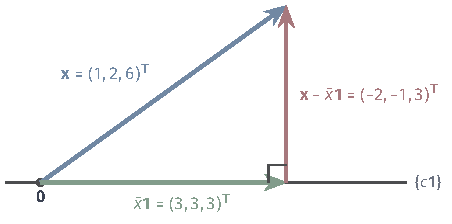
\includegraphics[width=77mm]{figures/07-probability/01-elementary-probability/tikz/mvd-mean-residual/figure.pdf}
  \caption{观测向量$\bm{x}=(1,2,6)^{\top}$（蓝）的正交分解，画在$\bm{1}$与$\bm{x}$张成的平面内并按比例绘制。绿色箭头是在直线$\{c\bm{1}\}$上的投影$\bar{x}\bm{1}$，红色箭头是残差$\bm{x}-\bar{x}\bm{1}$，两者垂直。}
  \label{fig:mvd-mean-residual}
\end{BookInlineFigure}

$(\bar{X}_n,\bm{R})$是$\bm{X}$的线性像，联合高斯。交叉协方差为
\[
 \operatorname{Cov}(\bm{R},\bar{X}_n)=\bm{P}\,(\sigma^{2}\bm{I}_n)\,\frac1n\bm{1}=\frac{\sigma^{2}}{n}\bm{P}\bm{1}=\bm{0} ,
\]
因为$\bm{P}\bm{1}=\bm{1}-\bm{1}=\bm{0}$。由定理~\ref{thm:mvd-gaussian-independence}，$\bar{X}_n$与整个残差向量独立，因而与残差平方和$\lVert\bm{R}\rVert_2^{2}$独立。

两部分的分布也能读出来。$\bar{X}_n\sim\mathcal{N}(\mu,\sigma^{2}/n)$。$\bm{R}\sim\mathcal{N}(\bm{0},\sigma^{2}\bm{P})$，$\bm{P}$是到$n-1$维子空间的正交投影，秩为$n-1$，所以$\bm{R}$是一个退化高斯向量，只在分量和为$0$的超平面上取值。

残差平方和的分布可以用旋转不变性求出。取正交矩阵$\bm{Q}$，其第一行为$\bm{1}^{\top}/\sqrt n$，令$\bm{Y}=\bm{Q}\bm{Z}$，由引理~\ref{lem:mvd-rotation}它仍是标准高斯向量，且$Y_1=\sqrt n\,\bar{Z}$，$\lVert\bm{Y}\rVert_2=\lVert\bm{Z}\rVert_2$。于是
\[
 \sum_{i=1}^{n}(Z_i-\bar{Z})^{2}=\lVert\bm{Z}\rVert_2^{2}-n\bar{Z}^{2}=\sum_{i=2}^{n}Y_i^{2} .
\]
右边是$n-1$个独立标准高斯变量的平方和，服从$\chi^2_{n-1}$（第~\ref{chap:random-variable-transformations}章），所以$\sum_i(X_i-\bar{X}_n)^{2}/\sigma^{2}\sim\chi^2_{n-1}$。样本平均与样本方差独立，是高斯模型统计推断的出发点，可参考\BookChapterRef{chap:parametric-statistical-inference}{卷八第1章“参数化统计推断”}。

这个独立性依赖联合高斯，不是样本平均与残差的一般性质。对任何有限方差的独立同分布样本，$\operatorname{Cov}(\bm{R},\bar{X}_n)=\bm{0}$都成立，但不相关推不出独立。图~\ref{fig:mvd-mean-variance}对比两种总体：高斯样本的平均与残差平方和看不出关系，指数样本的平均越大，残差平方和越分散。

\begin{BookInlineFigure}
  \centering
  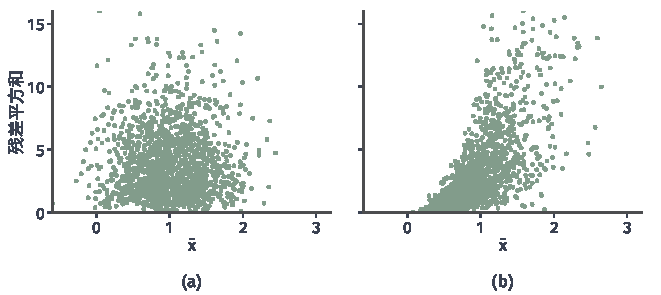
\includegraphics[width=112mm]{figures/07-probability/01-elementary-probability/matplotlib/mvd-mean-variance/figure.pdf}
  \caption{样本平均与残差平方和，每组$n=5$个观测，重复$1500$组。(a)$\mathcal{N}(1,1)$样本（种子$21$），两者的样本相关系数约为$0.02$。(b)$\operatorname{Exp}(1)$样本（均值与方差同为$1$，种子$22$），样本相关系数约为$0.68$，平均越大残差平方和越大。}
  \label{fig:mvd-mean-variance}
\end{BookInlineFigure}


\section{多元t分布}
\label{sec:mvd-t}

多元高斯的尾部很轻：传感器例子中，读数偏离均值超过三个标准差的机会只有千分之几。可是实际环境有时整体变得嘈杂，比如房间的空调启动，两台传感器的误差同时放大。这种“整体波动”不是加在某一台上的独立扰动，而是一个乘在所有分量上的共同尺度。

把多元高斯中固定的尺度换成随机的共同尺度，就得到多元t分布。本节先构造它并求出联合密度，再弄清位置、尺度矩阵和自由度三种参数的不同作用，最后说明共同尺度造成的依赖：即使尺度矩阵是对角的，分量也不独立。

一元情形已在第~\ref{chap:common-distributions}章出现：位置为$\mu$、尺度为$s>0$、自由度为$\nu>0$的t分布密度是
\[
 f(x)=\frac{\Gamma\bigl(\frac{\nu+1}{2}\bigr)}{\Gamma\bigl(\frac{\nu}{2}\bigr)\sqrt{\nu\pi}\,s}\Bigl(1+\frac{(x-\mu)^{2}}{\nu s^{2}}\Bigr)^{-(\nu+1)/2} ,
\]
$\nu=1$时就是Cauchy分布。下面的构造在$d=1$时回到它。

\subsection{正态尺度混合}
\label{sec:mvd-t-mixture}

\paragraph{构造}
取一个高斯向量和一个控制尺度的正随机变量，两者独立，用后者统一放大前者。为使结果的边缘回到一元t分布，尺度取为$\chi^2$变量倒数的平方根。

\begin{definition}[多元t分布]
\label{def:mvd-t}
设$\nu>0$，$\bm{\mu}\in\mathbb{R}^{d}$，$\bm{\Sigma}$是$d\times d$正定矩阵。$\bm{Z}\sim\mathcal{N}(\bm{0},\bm{\Sigma})$与$U\sim\chi^2_\nu$相互独立，令
\begin{equation}
 \bm{X}=\bm{\mu}+\sqrt{\nu/U}\,\bm{Z} .
 \label{eq:mvd-t-construction}
\end{equation}
称$\bm{X}$服从位置为$\bm{\mu}$、\term{尺度矩阵}（scale matrix）为$\bm{\Sigma}$、自由度为$\nu$的\term{多元t分布}（multivariate t distribution）。
\end{definition}

记$V=\sqrt{\nu/U}$。它对所有分量相同：$\bm{X}-\bm{\mu}=V\bm{Z}$的每个分量都乘以同一个$V$。这种把高斯向量乘上一个独立随机尺度的构造称为\term{正态尺度混合}（normal scale mixture）：固定$U=u$，$\bm{X}=\bm{\mu}+\sqrt{\nu/u}\,\bm{Z}$，由式~\eqref{eq:mvd-gaussian-affine}，
\[
 \bm{X}\text{在}U=u\text{时服从}\ \mathcal{N}\Bigl(\bm{\mu},\ \frac{\nu}{u}\bm{\Sigma}\Bigr) .
\]
$\bm{X}$的分布就是这些高斯分布按$U$的分布加权混合。

$U$的均值是$\nu$，所以$V$大致在$1$附近，但$U$可以很接近$0$，此时$V$很大，整个向量被大幅放大。图~\ref{fig:mvd-t-scale}(a)画出不同自由度下$V$的密度：$\nu=1$时$V$有很长的右尾，$\nu=30$时$V$已经紧紧围着$1$。

\paragraph{联合密度}
因为$\bm{Z}$与$U$独立，$(\bm{Z},U)$的联合密度是两者密度之积。对区域$S$，先对$\bm{z}$积分、再对$u$积分，
\[
 \mathbb{P}(\bm{X}\in S)=\int_0^{\infty}f_U(u)\,\mathbb{P}\Bigl(\bm{\mu}+\sqrt{\nu/u}\,\bm{Z}\in S\Bigr)\,\mathrm{d}u .
\]
括号里的概率是$\mathcal{N}(\bm{\mu},(\nu/u)\bm{\Sigma})$的密度在$S$上的积分。被积函数非负，可以交换两次积分的次序，于是$\bm{X}$有密度
\begin{equation}
 f_{\bm{X}}(\bm{x})=\int_0^{\infty}f_U(u)\,g_u(\bm{x})\,\mathrm{d}u ,
 \label{eq:mvd-scale-mixture-density}
\end{equation}
其中$g_u$是$\mathcal{N}(\bm{\mu},(\nu/u)\bm{\Sigma})$的密度。式~\eqref{eq:mvd-scale-mixture-density}对任何独立的正尺度都成立，下一节的多元Laplace分布也用它。

\begin{theorem}[多元t密度]
\label{thm:mvd-t-density}
定义~\ref{def:mvd-t}中的$\bm{X}$有联合密度
\begin{equation}
 f_{\bm{X}}(\bm{x})=\frac{\Gamma\bigl(\frac{\nu+d}{2}\bigr)}{\Gamma\bigl(\frac{\nu}{2}\bigr)(\nu\pi)^{d/2}(\det\bm{\Sigma})^{1/2}}\Bigl(1+\frac{Q(\bm{x})}{\nu}\Bigr)^{-(\nu+d)/2},
 \label{eq:mvd-t-density}
\end{equation}
其中$Q$由式~\eqref{eq:mvd-gaussian-quadratic}给出。
\end{theorem}

\begin{proof}
把$\bm{\Sigma}$换成$(\nu/u)\bm{\Sigma}$，式~\eqref{eq:mvd-gaussian-density}给出
\[
 g_u(\bm{x})=\frac{u^{d/2}}{(2\pi\nu)^{d/2}(\det\bm{\Sigma})^{1/2}}\exp\Bigl(-\frac{uQ}{2\nu}\Bigr) .
\]
$\chi^2_\nu=\operatorname{Gamma}(\nu/2,1/2)$，其密度为
\[
 f_U(u)=\frac{u^{\nu/2-1}\mathrm{e}^{-u/2}}{2^{\nu/2}\Gamma(\nu/2)},\qquad u>0 .
\]

两者相乘，$u$的幂次合并为$u^{(\nu+d)/2-1}$，指数合并为$-u(1+Q/\nu)/2$。由Gamma积分
\[
 \int_0^{\infty}u^{a-1}\mathrm{e}^{-bu}\,\mathrm{d}u=\Gamma(a)\,b^{-a},\qquad a,b>0,
\]
取$a=(\nu+d)/2$，$b=(1+Q/\nu)/2$，
\[
 \int_0^{\infty}u^{\frac{\nu+d}{2}-1}\mathrm{e}^{-\frac{u}{2}(1+Q/\nu)}\,\mathrm{d}u=\Gamma\Bigl(\frac{\nu+d}{2}\Bigr)\,2^{(\nu+d)/2}\Bigl(1+\frac{Q}{\nu}\Bigr)^{-(\nu+d)/2} .
\]
最后整理常数：$2^{(\nu+d)/2}$与$f_U$中的$2^{-\nu/2}$合成$2^{d/2}$，再与$(2\pi\nu)^{-d/2}$合成$(\nu\pi)^{-d/2}$。
\end{proof}

$d=1$、$\bm{\Sigma}=s^{2}$时，$Q=(x-\mu)^{2}/s^{2}$，式~\eqref{eq:mvd-t-density}就是本节开头的一元t密度。与高斯一样，密度只通过$Q$依赖$\bm{x}$，等密度面仍是以$\bm{\mu}$为中心、由$\bm{\Sigma}$决定形状的椭球；这类分布称为\term{椭圆分布}（elliptical distribution）。不同的是密度沿椭球向外的衰减方式：高斯是$\mathrm{e}^{-Q/2}$，t是$Q$的负幂。

取$d=2$、$\nu=5$、$\bm{\mu}=\bm{0}$、$\bm{\Sigma}=\bm{I}$，由$\Gamma(3.5)=2.5\,\Gamma(2.5)$，常数是
\[
 \frac{\Gamma(3.5)}{\Gamma(2.5)\cdot5\pi}=\frac{2.5}{5\pi}=\frac{1}{2\pi},
\]
中心密度恰好与二维标准高斯相同。在$Q=25$，也就是离中心$5$个单位处，两者分别是
\[
 \frac{1}{2\pi}\Bigl(1+\frac{25}{5}\Bigr)^{-7/2}\approx3.0\times10^{-4},\qquad \frac{1}{2\pi}\mathrm{e}^{-25/2}\approx5.9\times10^{-7} ,
\]
相差约$500$倍。

\begin{BookInlineFigure}
  \centering
  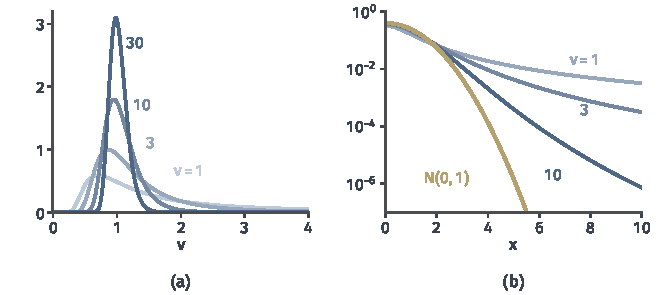
\includegraphics[width=112mm]{figures/07-probability/01-elementary-probability/matplotlib/mvd-t-scale/figure.pdf}
  \caption{共同尺度与尾部。(a)共同尺度$V=\sqrt{\nu/U}$的密度，$\nu=1,3,10,30$（蓝色由浅到深）；自由度越大，$V$越集中在$1$附近。(b)一个分量（$\Sigma_{i,i}=1$）的密度，纵轴取对数：t分布$\nu=1,3,10$（蓝色由浅到深）与$\mathcal{N}(0,1)$（黄）。}
  \label{fig:mvd-t-scale}
\end{BookInlineFigure}

\subsection{参数与矩}
\label{sec:mvd-t-moments}

\paragraph{位置与均值}
由构造，$\bm{X}-\bm{\mu}=V\bm{Z}$关于$\bm{\mu}$对称：$V\bm{Z}$与$-V\bm{Z}$同分布。所以$\bm{\mu}$总是分布的对称中心，也是每个分量的中位数。它是不是均值，要看$\bm{X}$的分量是否可积。

由$V$与$\bm{Z}$独立，
\[
 \mathbb{E}\lvert X_i-\mu_i\rvert=\mathbb{E}[V]\,\mathbb{E}\lvert Z_i\rvert ,
\]
而$\mathbb{E}\lvert Z_i\rvert$有限且为正。对$V$的矩，设$k\geq0$，由$U$的密度，
\[
 \mathbb{E}\bigl[U^{-k/2}\bigr]=\int_0^{\infty}\frac{u^{\nu/2-k/2-1}\mathrm{e}^{-u/2}}{2^{\nu/2}\Gamma(\nu/2)}\,\mathrm{d}u
\]
的有限性只取决于原点附近：积分在$0$附近收敛当且仅当$\nu/2-k/2>0$。

所以$\mathbb{E}[V^{k}]=\nu^{k/2}\mathbb{E}[U^{-k/2}]$在$k<\nu$时有限，在$k\geq\nu$时为无穷，从而
\[
 \mathbb{E}\lvert X_i-\mu_i\rvert^{k}<\infty\quad\Longleftrightarrow\quad k<\nu .
\]
特别地，$\nu>1$时均值存在，由$\mathbb{E}[\bm{Z}]=\bm{0}$，均值等于$\bm{\mu}$；$\nu\leq1$时均值不存在，$\bm{\mu}$只是位置。Cauchy情形$\nu=1$就是这样。

\paragraph{尺度矩阵与协方差}
$k=2$时，算出Gamma积分得
\[
 \mathbb{E}[1/U]=\frac{\Gamma(\nu/2-1)}{2\Gamma(\nu/2)}=\frac{1}{\nu-2},\qquad \nu>2 .
\]
于是$\nu>2$时
\begin{equation}
 \operatorname{Cov}(\bm{X})=\mathbb{E}[V^{2}]\,\operatorname{Cov}(\bm{Z})=\frac{\nu}{\nu-2}\,\bm{\Sigma} .
 \label{eq:mvd-t-cov}
\end{equation}
所以$\bm{\Sigma}$不是协方差矩阵，而是尺度矩阵：它决定椭球的形状和方向，协方差还要乘以共同尺度的二阶矩。两者只差一个正数倍，相关系数矩阵相同。

各种矩的存在条件按自由度列在表~\ref{tab:mvd-t-moments}中。

\begin{BookInlineTable}
  \centering
  \begin{tabular}{lcccc}
    \toprule
    自由度 & $0<\nu\leq1$ & $1<\nu\leq2$ & $2<\nu\leq4$ & $\nu>4$\\
    \midrule
    均值$\bm{\mu}$ & 不存在 & 存在 & 存在 & 存在\\
    协方差 & 不存在 & 不存在 & $\frac{\nu}{\nu-2}\bm{\Sigma}$ & $\frac{\nu}{\nu-2}\bm{\Sigma}$\\
    四阶矩 & 不存在 & 不存在 & 不存在 & 存在\\
    \bottomrule
  \end{tabular}
  \caption{多元t分布各阶矩的存在条件，“存在”指对应的期望有限。}
  \label{tab:mvd-t-moments}
\end{BookInlineTable}

\paragraph{边缘与线性组合}
取出第$i$个分量，$X_i=\mu_i+VZ_i$，$Z_i\sim\mathcal{N}(0,\Sigma_{i,i})$，$V$不变。这正是$d=1$时的同一构造，所以$X_i$服从位置$\mu_i$、尺度$\sqrt{\Sigma_{i,i}}$、自由度$\nu$的一元t分布。同理，$\bm{a}^{\top}\bm{X}$等于$\bm{a}^{\top}\bm{\mu}$加上$V\,\bm{a}^{\top}\bm{Z}$，服从尺度为$\sqrt{\bm{a}^{\top}\bm{\Sigma}\bm{a}}$的一元t分布，任意一组分量服从相应子矩阵的多元t分布。边缘与整体的自由度相同，因为它们共用同一个$U$。

一元t密度的尾部按$\lvert x\rvert^{-(\nu+1)}$衰减，所以$\nu$越小尾部越重，图~\ref{fig:mvd-t-scale}(b)。由上面的矩条件，这与“$k\geq\nu$阶矩不存在”是一回事：尾部太重，高阶矩积不出来。

\paragraph{自由度增大时}
$U\sim\chi^2_\nu$的均值为$\nu$、方差为$2\nu$，所以$U/\nu$的均值为$1$、方差为$2/\nu$。由第~\ref{chap:tail-probabilities}章的Chebyshev不等式，对任意$\varepsilon>0$，
\[
 \mathbb{P}\Bigl(\Bigl\lvert\frac{U}{\nu}-1\Bigr\rvert\geq\varepsilon\Bigr)\leq\frac{2}{\nu\varepsilon^{2}} .
\]
$\nu\to\infty$时右边趋于$0$，共同尺度$V=(U/\nu)^{-1/2}$越来越确定地接近$1$，$\bm{X}$也就越来越像$\mathcal{N}(\bm{\mu},\bm{\Sigma})$。从密度看，$(1+Q/\nu)^{-(\nu+d)/2}\to\mathrm{e}^{-Q/2}$，常数也趋于高斯的常数。$\nu$因此度量了“尺度有多不确定”：自由度小，尺度波动大，尾部重；自由度大，模型退回高斯。

\subsection{分量的依赖}
\label{sec:mvd-t-dependence}

设$\bm{\Sigma}$是对角矩阵，为简单起见取$\bm{\mu}=\bm{0}$、$\bm{\Sigma}=\bm{I}_d$。固定$U=u$时，$\bm{X}\sim\mathcal{N}(\bm{0},(\nu/u)\bm{I}_d)$，各分量相互独立：给定共同尺度，分量条件独立。$\nu>2$时由式~\eqref{eq:mvd-t-cov}，协方差矩阵也是对角的，分量两两不相关。可是不知道$U$的时候，一个分量很大，说明共同尺度可能很大，另一个分量也就更可能大。

\paragraph{联合密度不能分解}
先证明，对任何$\nu>0$，$d=2$时$X_1$与$X_2$不独立。若两者独立，对以$(x_1,x_2)$为中心、边长为$h$的小正方形，联合概率等于两个边长为$h$的区间概率之积。两边除以$h^{2}$，令$h\to0$，由三个密度的连续性得到
\[
 f_{\bm{X}}(x_1,x_2)=f_{X_1}(x_1)\,f_{X_2}(x_2)\qquad\text{对一切}(x_1,x_2) .
\]
于是对任意$a,b$，必须有
\[
 f_{\bm{X}}(a,b)\,f_{\bm{X}}(0,0)=f_{\bm{X}}(a,0)\,f_{\bm{X}}(0,b) ,
\]
因为两边都等于同样四个边缘密度值之积。

取$a=b=1$检验。由式~\eqref{eq:mvd-t-density}，$f_{\bm{X}}$与$k(Q)=(1+Q/\nu)^{-(\nu+2)/2}$成正比，上式要求$k(2)k(0)=k(1)^{2}$。但
\[
 \Bigl(1+\frac1\nu\Bigr)^{2}=1+\frac2\nu+\frac{1}{\nu^{2}}>1+\frac2\nu ,
\]
两边取$-(\nu+2)/2$次幂，不等号反向，得到$k(1)^{2}<k(2)=k(2)k(0)$。等式不成立，所以$X_1$与$X_2$不独立。

\paragraph{条件方差随观测增大}
依赖的方式可以算得很具体。固定$X_1=x_1$，把联合密度看成$x_2$的函数并提出与$x_2$无关的因子：
\[
 \Bigl(1+\frac{x_1^{2}+x_2^{2}}{\nu}\Bigr)^{-\frac{\nu+2}{2}}=\Bigl(1+\frac{x_1^{2}}{\nu}\Bigr)^{-\frac{\nu+2}{2}}\Bigl(1+\frac{x_2^{2}}{\nu+x_1^{2}}\Bigr)^{-\frac{\nu+2}{2}} .
\]
第二个因子正是自由度$\nu+1$、尺度$s$满足$(\nu+1)s^{2}=\nu+x_1^{2}$的一元t密度的形状。

所以给定$X_1=x_1$，$X_2$服从自由度$\nu+1$、尺度平方为$(\nu+x_1^{2})/(\nu+1)$的t分布。$\nu>1$时它的自由度大于$2$，由式~\eqref{eq:mvd-t-cov}的一元情形，
\begin{equation}
 \mathbb{E}[X_2^{2}\mid X_1=x_1]=\frac{\nu+x_1^{2}}{\nu+1}\cdot\frac{\nu+1}{\nu-1}=\frac{\nu+x_1^{2}}{\nu-1} .
 \label{eq:mvd-t-conditional-second-moment}
\end{equation}
它随$\lvert x_1\rvert$增大而增大。

取$\nu=5$：$X_2$的无条件方差是$5/3\approx1.67$；观测到$x_1=0$时条件二阶矩是$5/4=1.25$，观测到$x_1=3$时变为$14/4=3.5$。第一个分量平静，说明共同尺度多半不大，第二个分量也收敛一些；第一个分量剧烈，第二个分量的波动随之放大。图~\ref{fig:mvd-t-dependence}(b)用模拟样本核对了式~\eqref{eq:mvd-t-conditional-second-moment}。

\begin{BookInlineFigure}
  \centering
  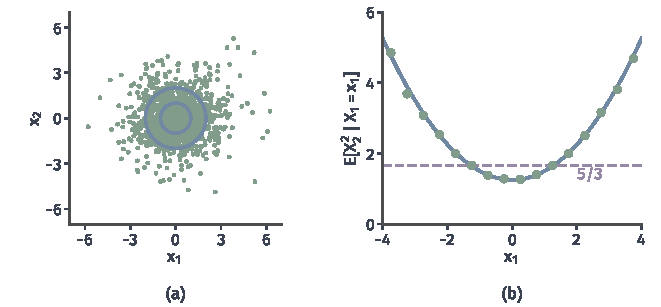
\includegraphics[width=112mm]{figures/07-probability/01-elementary-probability/matplotlib/mvd-t-dependence/figure.pdf}
  \caption{$\nu=5$、$\bm{\Sigma}=\bm{I}$的二维t分布，分量不相关但不独立。(a)$1500$个样本（绿，种子$31$）与等密度圆$Q=1,4$（蓝）；远处的点往往两个坐标同时偏大。(b)条件二阶矩$\mathbb{E}[X_2^{2}\mid X_1=x_1]=(5+x_1^{2})/4$（蓝），绿点是$40$万个样本（种子$32$）按$x_1$分组、组宽$0.5$的组内平均，紫色虚线是无条件方差$5/3$。}
  \label{fig:mvd-t-dependence}
\end{BookInlineFigure}

\paragraph{平方的协方差}
同样的依赖也能从矩看出来。$\nu>4$时$\mathbb{E}[1/U^{2}]=1/((\nu-2)(\nu-4))$，由$V$与$\bm{Z}$独立及$Z_1,Z_2$独立，
\[
 \mathbb{E}[X_1^{2}X_2^{2}]=\mathbb{E}[V^{4}]\,\mathbb{E}[Z_1^{2}]\,\mathbb{E}[Z_2^{2}]=\frac{\nu^{2}}{(\nu-2)(\nu-4)} .
\]
而$\mathbb{E}[X_1^{2}]$与$\mathbb{E}[X_2^{2}]$都等于$\nu/(\nu-2)$，两者之差为
\[
 \operatorname{Cov}(X_1^{2},X_2^{2})=\frac{2\nu^{2}}{(\nu-2)^{2}(\nu-4)}>0 .
\]
$\nu=5$时它等于$50/9\approx5.56$。$X_1$与$X_2$不相关，$X_1^{2}$与$X_2^{2}$却正相关：共同尺度让两个分量的大小一起涨落，而符号仍各自随机，所以线性的协方差看不到这种依赖。

如果想要“边缘是t分布、分量独立”的模型，就应让每个分量各用一个独立的尺度：$X_i=\mu_i+\sqrt{\nu/U_i}\,Z_i$，$U_1,\ldots,U_d$相互独立。它的边缘与多元t相同，协方差也相同，却是另一个联合分布，等密度线不再是椭圆。第~\ref{sec:mvd-comparison}节会比较两种模型在“同时出现大值”上的差别。


\section{多元Laplace分布}
\label{sec:mvd-laplace}

t分布的重尾有代价：自由度小的时候，方差甚至均值都不存在。有些波动比高斯更“尖”、尾部更厚，却仍有全部有限阶矩，一元时第~\ref{chap:common-distributions}章的Laplace分布正适合描述它们。它的密度是$(2b)^{-1}\mathrm{e}^{-\lvert x-\mu\rvert/b}$，尾部按指数衰减，比高斯的$\mathrm{e}^{-x^{2}/2}$慢，但仍快过任何负幂。

推广到多元，答案并不唯一。最直接的做法是让各分量独立地服从一元Laplace分布；另一种做法沿用上一节的思路，用一个共同的随机尺度放大高斯向量。本节采用后者，即由共同指数尺度混合得到的对称椭圆型版本，称为\term{多元Laplace分布}（multivariate Laplace distribution），并在最后与独立分量的乘积模型对照。

\subsection{正态指数混合}
\label{sec:mvd-laplace-mixture}

\paragraph{构造}
上一节的共同尺度$\nu/U$有很长的右尾，这是t分布矩不存在的根源。换一个右尾短的尺度，就能保留混合带来的厚尾，又不丢掉矩。指数分布是最简单的选择。

\begin{definition}[多元Laplace分布]
\label{def:mvd-laplace}
设$\bm{\mu}\in\mathbb{R}^{d}$，$\bm{\Sigma}$是$d\times d$正定矩阵。$W\sim\operatorname{Exp}(1)$（速率为$1$）与$\bm{Z}\sim\mathcal{N}(\bm{0},\bm{\Sigma})$相互独立，令
\begin{equation}
 \bm{X}=\bm{\mu}+\sqrt{W}\,\bm{Z} .
 \label{eq:mvd-laplace-construction}
\end{equation}
称$\bm{X}$服从参数为$\bm{\mu}$、$\bm{\Sigma}$的多元Laplace分布。
\end{definition}

固定$W=w$，$\bm{X}\sim\mathcal{N}(\bm{\mu},w\bm{\Sigma})$，所以这仍是一个正态尺度混合，只是这次混合的是方差因子$W$本身。图~\ref{fig:mvd-mixing-laws}比较两种方差因子：$\nu=5$的t分布用$5/U$，本节用$W$。两者都可以取远大于$1$的值，这是厚尾的来源；但$W$的尾概率是$\mathrm{e}^{-v}$，$5/U$的尾概率只按$v^{-5/2}$下降。

\begin{BookInlineFigure}
  \centering
  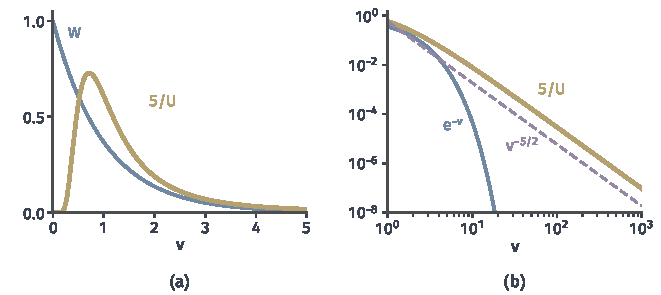
\includegraphics[width=112mm]{figures/07-probability/01-elementary-probability/matplotlib/mvd-mixing-laws/figure.pdf}
  \caption{两种正态尺度混合的方差因子。(a)密度：多元Laplace的$W\sim\operatorname{Exp}(1)$（蓝）与$\nu=5$的多元t的$5/U$，$U\sim\chi^2_5$（黄）。(b)尾概率$\mathbb{P}(\cdot>v)$，双对数坐标；紫色虚线是斜率为$-5/2$的参考线。尾概率由精确密度数值积分得到。}
  \label{fig:mvd-mixing-laws}
\end{BookInlineFigure}

\paragraph{均值、协方差与矩}
$\sqrt W$的均值$\Gamma(3/2)=\sqrt\pi/2$有限，由独立性及$\mathbb{E}[\bm{Z}]=\bm{0}$，$\mathbb{E}[\bm{X}]=\bm{\mu}$。协方差为
\begin{equation}
 \operatorname{Cov}(\bm{X})=\mathbb{E}[W]\,\bm{\Sigma}=\bm{\Sigma} .
 \label{eq:mvd-laplace-cov}
\end{equation}
与t分布不同，这里的$\bm{\Sigma}$就是协方差矩阵。

更高阶的矩同样存在。对任意$k\geq0$，$\mathbb{E}[W^{k/2}]=\Gamma(1+k/2)<\infty$，而高斯分量的各阶矩都有限，所以
\[
 \mathbb{E}\lvert X_i-\mu_i\rvert^{k}=\Gamma\Bigl(1+\frac k2\Bigr)\,\mathbb{E}\lvert Z_i\rvert^{k}<\infty .
\]
这正是选用指数尺度的目的：混合让尾部变厚，指数尺度的短尾又保证一切矩有限。

\paragraph{联合密度}
由式~\eqref{eq:mvd-scale-mixture-density}，把$g_u$换成$\mathcal{N}(\bm{\mu},w\bm{\Sigma})$的密度、$f_U$换成$\mathrm{e}^{-w}$，
\begin{equation}
 f_{\bm{X}}(\bm{x})=\frac{1}{(2\pi)^{d/2}(\det\bm{\Sigma})^{1/2}}\int_0^{\infty}w^{-d/2}\exp\Bigl(-w-\frac{Q(\bm{x})}{2w}\Bigr)\,\mathrm{d}w .
 \label{eq:mvd-laplace-density}
\end{equation}
密度仍只通过$Q(\bm{x})$依赖$\bm{x}$，所以多元Laplace分布也是椭圆分布，等密度面与$\mathcal{N}(\bm{\mu},\bm{\Sigma})$的相同。剩下的问题是沿着椭球向外，密度怎样衰减。下面的积分让我们在$d=1$和$d=3$时算出初等形式。

\begin{lemma}[一个指数积分]
\label{lem:mvd-exp-integral}
对$a>0$，
\begin{equation}
 \begin{aligned}
  \int_0^{\infty}w^{-1/2}\mathrm{e}^{-w-a/w}\,\mathrm{d}w&=\sqrt\pi\,\mathrm{e}^{-2\sqrt a},\\
  \int_0^{\infty}w^{-3/2}\mathrm{e}^{-w-a/w}\,\mathrm{d}w&=\sqrt{\frac{\pi}{a}}\,\mathrm{e}^{-2\sqrt a} .
 \end{aligned}
 \label{eq:mvd-exp-integral}
\end{equation}
\end{lemma}

\begin{proof}
第一个积分中令$w=s^{2}$，$\mathrm{d}w=2s\,\mathrm{d}s$，再记$c=\sqrt a$并在指数中配方，$s^{2}+c^{2}/s^{2}=(s-c/s)^{2}+2c$，于是
\[
 \int_0^{\infty}w^{-1/2}\mathrm{e}^{-w-a/w}\,\mathrm{d}w=2\int_0^{\infty}\mathrm{e}^{-s^{2}-c^{2}/s^{2}}\,\mathrm{d}s=2\mathrm{e}^{-2c}J,
\]
其中
\[
 J=\int_0^{\infty}\mathrm{e}^{-(s-c/s)^{2}}\,\mathrm{d}s .
\]

求$J$用一个对称技巧。令$s=c/t$，$\mathrm{d}s=-c\,t^{-2}\mathrm{d}t$，积分限对调，$(s-c/s)^{2}=(c/t-t)^{2}$，所以
\[
 J=\int_0^{\infty}\mathrm{e}^{-(t-c/t)^{2}}\,\frac{c}{t^{2}}\,\mathrm{d}t .
\]
把两种写法相加，
\[
 2J=\int_0^{\infty}\mathrm{e}^{-(s-c/s)^{2}}\Bigl(1+\frac{c}{s^{2}}\Bigr)\,\mathrm{d}s .
\]
再令$y=s-c/s$，它在$(0,\infty)$上严格递增，从$-\infty$变到$\infty$，且$\mathrm{d}y=(1+c/s^{2})\,\mathrm{d}s$，
\[
 2J=\int_{-\infty}^{\infty}\mathrm{e}^{-y^{2}}\,\mathrm{d}y=\sqrt\pi .
\]
所以$J=\sqrt\pi/2$，第一个等式成立。

第二个积分由第一个换元得到。在第一个积分中令$w=a/t$，$\mathrm{d}w=-a\,t^{-2}\mathrm{d}t$，$w^{-1/2}=t^{1/2}a^{-1/2}$，指数$-w-a/w$变为$-a/t-t$，于是
\[
 \sqrt\pi\,\mathrm{e}^{-2\sqrt a}=\int_0^{\infty}t^{1/2}a^{-1/2}\,\mathrm{e}^{-t-a/t}\,\frac{a}{t^{2}}\,\mathrm{d}t=\sqrt a\int_0^{\infty}t^{-3/2}\mathrm{e}^{-t-a/t}\,\mathrm{d}t .
\]
两边除以$\sqrt a$即得第二个等式。
\end{proof}

$d=1$时$\bm{\Sigma}=\sigma^{2}$，$Q=(x-\mu)^{2}/\sigma^{2}$。式~\eqref{eq:mvd-laplace-density}中取$a=Q/2$，用式~\eqref{eq:mvd-exp-integral}的第一式，$2\sqrt a=\sqrt2\,\lvert x-\mu\rvert/\sigma$，
\[
 f_X(x)=\frac{1}{\sqrt{2\pi}\,\sigma}\sqrt\pi\,\mathrm{e}^{-\sqrt2\lvert x-\mu\rvert/\sigma}=\frac{1}{\sqrt2\,\sigma}\mathrm{e}^{-\sqrt2\lvert x-\mu\rvert/\sigma} .
\]
这正是尺度$b=\sigma/\sqrt2$的一元Laplace密度，其方差$2b^{2}=\sigma^{2}$与式~\eqref{eq:mvd-laplace-cov}一致。

$d=3$时用第二式，同样取$a=Q/2$，常数$(2\pi)^{-3/2}\sqrt{2\pi}=(2\pi)^{-1}$，得到
\[
 f_{\bm{X}}(\bm{x})=\frac{1}{2\pi(\det\bm{\Sigma})^{1/2}}\cdot\frac{\mathrm{e}^{-\sqrt{2Q(\bm{x})}}}{\sqrt{Q(\bm{x})}} .
\]
它不只是$\mathrm{e}^{-\sqrt{2Q}}$：多出的因子$Q^{-1/2}$让密度在中心$\bm{x}=\bm{\mu}$处趋于无穷。

\paragraph{中心的奇性}
$d\geq2$时中心的奇性是普遍的，不依赖初等形式。若$Q(\bm{x})\leq\varepsilon<1$，式~\eqref{eq:mvd-laplace-density}中的积分只保留$w\in[\varepsilon,1]$一段，在这一段上$\mathrm{e}^{-w}\geq\mathrm{e}^{-1}$，$Q/(2w)\leq\tfrac12$，于是
\[
 \int_0^{\infty}w^{-d/2}\mathrm{e}^{-w-Q/(2w)}\,\mathrm{d}w\geq\mathrm{e}^{-3/2}\int_{\varepsilon}^{1}w^{-d/2}\,\mathrm{d}w .
\]
$d\geq2$时右边在$\varepsilon\to0$时趋于无穷，所以$\bm{x}\to\bm{\mu}$时$f_{\bm{X}}(\bm{x})\to\infty$。原因是$W$可以很接近$0$：此时高斯分量被压得很窄，在中心堆出越来越高的尖峰，维数越高，这些尖峰叠加得越陡。

奇性不影响概率的计算，密度仍然可积，总积分为$1$。它提醒我们：多元Laplace的密度沿椭球向外不是简单的$\mathrm{e}^{-\sqrt{2Q}}$，只有$d=1$时才是。把密度直接设成$c\,\mathrm{e}^{-\sqrt{2Q}}$得到的是另一个模型，与本节由共同指数尺度给出的构造不同。图~\ref{fig:mvd-laplace-shape}(b)沿一条射线画出$d=1,2,3$时的密度，$d=2$时的积分不是初等函数，由数值积分得到。

\begin{BookInlineFigure}
  \centering
  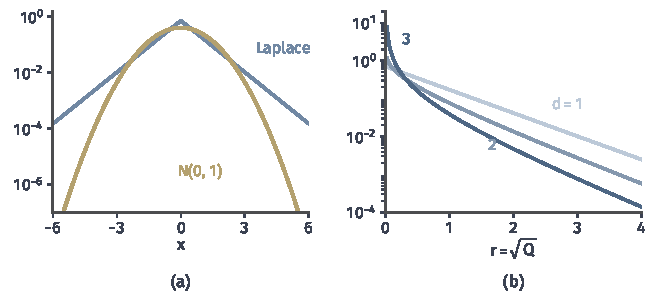
\includegraphics[width=112mm]{figures/07-probability/01-elementary-probability/matplotlib/mvd-laplace-shape/figure.pdf}
  \caption{多元Laplace的形状，$\bm{\mu}=\bm{0}$，$\bm{\Sigma}=\bm{I}_d$，纵轴取对数。(a)一个分量的密度：尺度$b=1/\sqrt2$的Laplace密度（蓝）与方差同为$1$的$\mathcal{N}(0,1)$密度（黄）；Laplace在中心更尖，在远处更厚。(b)沿射线的联合密度随$r=\sqrt Q$的变化，$d=1,2,3$（蓝色由浅到深），由式~\eqref{eq:mvd-laplace-density}数值积分；$d=2,3$时中心处趋于无穷。}
  \label{fig:mvd-laplace-shape}
\end{BookInlineFigure}

\subsection{边缘与共同尺度}
\label{sec:mvd-laplace-marginal}

\paragraph{边缘是一元Laplace}
取出第$i$个分量，$X_i=\mu_i+\sqrt W\,Z_i$，$Z_i\sim\mathcal{N}(0,\Sigma_{i,i})$，$W$不变。这就是$d=1$的构造，由上面的计算，$X_i$服从位置$\mu_i$、尺度
\begin{equation}
 b_i=\sqrt{\Sigma_{i,i}/2}
 \label{eq:mvd-laplace-marginal-scale}
\end{equation}
的一元Laplace分布，尺度的含义与第~\ref{chap:common-distributions}章相同。同理，$\bm{a}^{\top}\bm{X}$服从尺度为$\sqrt{\bm{a}^{\top}\bm{\Sigma}\bm{a}/2}$的一元Laplace分布，任意一组分量服从相应子矩阵的多元Laplace分布。

与同方差的高斯相比，Laplace边缘在中心更尖、远处更厚。图~\ref{fig:mvd-laplace-shape}(a)中两者方差都是$1$：Laplace在$0$处的密度是$1/\sqrt2\approx0.707$，高斯是$0.399$；而$\mathbb{P}(\lvert X_i\rvert>3)$，Laplace为$\mathrm{e}^{-3\sqrt2}\approx0.0144$，高斯约为$0.0027$。

\paragraph{共同尺度造成依赖}
取$\bm{\mu}=\bm{0}$、$\bm{\Sigma}=\bm{I}_2$。两个分量的协方差为$0$，边缘都是尺度$1/\sqrt2$的Laplace分布。它们是否独立？看中心化分量的交叉四阶矩。由$W$、$Z_1$、$Z_2$相互独立，
\[
 \mathbb{E}[X_1^{2}X_2^{2}]=\mathbb{E}[W^{2}]\,\mathbb{E}[Z_1^{2}]\,\mathbb{E}[Z_2^{2}]=2 ,
\]
这里用了$\mathbb{E}[W^{2}]=\Gamma(3)=2$。而$\mathbb{E}[X_1^{2}]\,\mathbb{E}[X_2^{2}]=1$。

若$X_1$与$X_2$独立，则$X_1^{2}$与$X_2^{2}$独立，乘积的期望应等于期望之积。现在$2\neq1$，所以两者不独立，$\operatorname{Cov}(X_1^{2},X_2^{2})=1>0$。与t分布一样，共同尺度$W$同时放大或缩小两个分量的大小，而符号由$Z_1$、$Z_2$独立决定，协方差看不到这种依赖。

\paragraph{与乘积模型对照}
现在另取两个独立的尺度，$Y_i=\sqrt{W_i}\,Z_i$，$W_1,W_2,Z_1,Z_2$相互独立。由一元计算，$Y_1$、$Y_2$也是尺度$1/\sqrt2$的Laplace变量，而且相互独立，联合密度是边缘之积，
\[
 f_{\bm{Y}}(y_1,y_2)=\frac12\exp\bigl(-\sqrt2(\lvert y_1\rvert+\lvert y_2\rvert)\bigr) .
\]
两个模型的边缘相同，均值都是$\bm{0}$，协方差矩阵都是$\bm{I}_2$。

可是它们的联合分布不同。乘积模型的交叉四阶矩是$\mathbb{E}[Y_1^{2}]\,\mathbb{E}[Y_2^{2}]=1$，不是$2$。几何上，椭圆型模型的等密度线是圆，乘积模型的等密度线是菱形$\lvert y_1\rvert+\lvert y_2\rvert=c$，图~\ref{fig:mvd-laplace-contours}。菱形的尖角落在坐标轴上：乘积模型容易出现“一个分量大、另一个分量小”的点；椭圆型模型的大值往往两个分量一起出现。

\begin{BookInlineFigure}
  \centering
  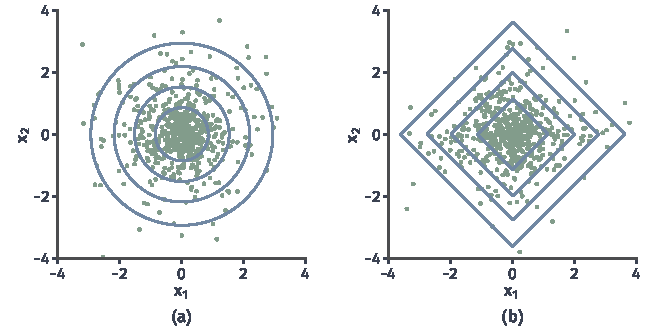
\includegraphics[width=112mm]{figures/07-probability/01-elementary-probability/matplotlib/mvd-laplace-contours/figure.pdf}
  \caption{边缘与协方差都相同的两个模型，各分量都是尺度$1/\sqrt2$的Laplace分布，协方差矩阵为$\bm{I}_2$。(a)椭圆型多元Laplace，等密度线是圆。(b)独立分量的乘积模型，等密度线是菱形。蓝线是密度等于$0.1,0.03,0.01,0.003$的等值线，绿点是各$600$个样本（种子$41$、$42$）。}
  \label{fig:mvd-laplace-contours}
\end{BookInlineFigure}

选哪一个版本，取决于数据的生成方式。各坐标的波动来自同一个源头，比如整个系统的状态忽强忽弱，椭圆型更合适；各坐标各自独立地出现尖峰，乘积模型更合适。两者都可以称为“多元Laplace”，使用时要说明采用的是哪一种构造。


\section{Dirichlet分布}
\label{sec:mvd-dirichlet}

甜品店的三种口味，选择概率$(0.5,0.3,0.2)$并不是一成不变的：天气、节日、新品都会让这天的偏好与那天不同。若把每天的偏好本身看成随机的，就得到一个随机的比例向量$\bm{P}=(P_1,P_2,P_3)^{\top}$，分量非负、和为$1$。一份混合物中各成分所占的比例，也是这样的对象。

这类对象与计数不同。多项分布中$\bm{p}$是给定的参数，随机的是计数；这里随机的是比例本身。两层可以叠加：先随机产生当天的偏好$\bm{P}$，再在给定$\bm{P}$时产生多项计数。本节只讨论比例的分布本身。由观测到的计数反过来更新对比例的认识，属于统计推断，归卷八。

一元时，第~\ref{chap:common-distributions}章的Beta分布描述$(0,1)$中的一个随机比例，另一类的比例就是它的补数。Dirichlet分布把它推广到$d$个类别。我们先说明它住在什么地方、密度相对于什么坐标，再用独立Gamma变量构造它，最后计算均值与协方差。

\subsection{单纯形上的密度}
\label{sec:mvd-dirichlet-density}

\paragraph{取值范围}
$d$个类别的比例向量取值于\term{标准单纯形}（standard simplex）
\[
 \Delta_{d-1}=\Bigl\{\bm{p}\in\mathbb{R}^{d}:\ p_i\geq0,\ \sum_{i=1}^{d}p_i=1\Bigr\} .
\]
$d=3$时它是$\mathbb{R}^{3}$中以三个坐标向量为顶点的三角形，图~\ref{fig:mvd-simplex}左侧；下标$d-1$是它的维数。

$\Delta_{d-1}$落在超平面$\sum_ip_i=1$里，$d$维体积为$0$，所以$\bm{P}$不可能有普通的$d$维密度，理由与退化高斯相同。办法是只用前$d-1$个分量作坐标，最后一个由$p_d=1-p_1-\cdots-p_{d-1}$确定。这些自由坐标取值于
\[
 T_{d-1}=\Bigl\{(p_1,\ldots,p_{d-1}):\ p_i>0,\ \sum_{i=1}^{d-1}p_i<1\Bigr\} ,
\]
$d=3$时是平面上的直角三角形，图~\ref{fig:mvd-simplex}右侧。密度就是$(P_1,\ldots,P_{d-1})$在$T_{d-1}$上的普通密度。

\begin{BookInlineFigure}
  \centering
  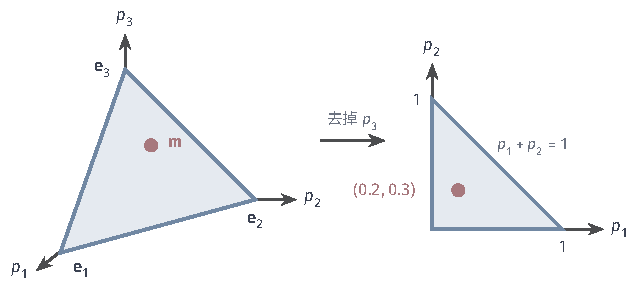
\includegraphics[width=109mm]{figures/07-probability/01-elementary-probability/tikz/mvd-simplex/figure.pdf}
  \caption{三个类别的比例。左：$\mathbb{R}^{3}$中的标准单纯形$\Delta_2$（浅蓝三角形），顶点为$\bm{e}_1,\bm{e}_2,\bm{e}_3$，红点$\bm{m}=(0.2,0.3,0.5)$。右：去掉$p_3$后的自由坐标区域$T_2$，红点是$\bm{m}$的像$(0.2,0.3)$。}
  \label{fig:mvd-simplex}
\end{BookInlineFigure}

\paragraph{密度与归一化}
Beta密度$t^{\alpha_1-1}(1-t)^{\alpha_2-1}$在$t$接近$0$时由$\alpha_1$控制，接近$1$时由$\alpha_2$控制。多个类别时，对每个比例都放一个这样的幂因子。

\begin{definition}[Dirichlet分布]
\label{def:mvd-dirichlet}
设$d\geq2$，$\bm{\alpha}=(\alpha_1,\ldots,\alpha_d)^{\top}$的各分量$\alpha_i>0$，记$\alpha_0=\alpha_1+\cdots+\alpha_d$。若随机向量$\bm{P}$取值于$\Delta_{d-1}$，且$(P_1,\ldots,P_{d-1})$在$T_{d-1}$上有密度
\begin{equation}
 f(p_1,\ldots,p_{d-1})=\frac{\Gamma(\alpha_0)}{\Gamma(\alpha_1)\cdots\Gamma(\alpha_d)}\prod_{i=1}^{d}p_i^{\alpha_i-1},\qquad p_d=1-\sum_{i=1}^{d-1}p_i ,
 \label{eq:mvd-dirichlet-density}
\end{equation}
则称$\bm{P}$服从参数为$\bm{\alpha}$的\term{Dirichlet分布}（Dirichlet distribution），记为$\bm{P}\sim\operatorname{Dir}(\bm{\alpha})$。
\end{definition}

$d=2$时，$P_1$在$(0,1)$上的密度是$\Gamma(\alpha_1+\alpha_2)/(\Gamma(\alpha_1)\Gamma(\alpha_2))\cdot p_1^{\alpha_1-1}(1-p_1)^{\alpha_2-1}$，就是$\operatorname{Beta}(\alpha_1,\alpha_2)$。第~\ref{chap:common-distributions}章的归一化等价于Beta积分
\[
 \int_0^{1}t^{a-1}(1-t)^{b-1}\,\mathrm{d}t=\frac{\Gamma(a)\Gamma(b)}{\Gamma(a+b)},\qquad a,b>0 .
\]
一般的$d$需要验证式~\eqref{eq:mvd-dirichlet-density}的积分为$1$，下面用归纳法从Beta积分推出。

\begin{lemma}[Dirichlet积分]
\label{lem:mvd-dirichlet-integral}
对$d\geq2$及正数$\alpha_1,\ldots,\alpha_d$，
\begin{equation}
 \int_{T_{d-1}}\prod_{i=1}^{d}p_i^{\alpha_i-1}\,\mathrm{d}p_1\cdots\mathrm{d}p_{d-1}=\frac{\Gamma(\alpha_1)\cdots\Gamma(\alpha_d)}{\Gamma(\alpha_0)} ,
 \label{eq:mvd-dirichlet-integral}
\end{equation}
其中$p_d=1-\sum_{i<d}p_i$。
\end{lemma}

\begin{proof}
$d=2$就是Beta积分。设结论对$d-1$成立，$d\geq3$。被积函数非负，可以先对$p_{d-1}$积分。固定$p_1,\ldots,p_{d-2}$，记$s=p_1+\cdots+p_{d-2}<1$，则$p_{d-1}$的范围是$(0,1-s)$，$p_d=1-s-p_{d-1}$。

令$p_{d-1}=(1-s)t$，$t\in(0,1)$，则$p_d=(1-s)(1-t)$，$\mathrm{d}p_{d-1}=(1-s)\,\mathrm{d}t$，于是
\[
 \int_0^{1-s}p_{d-1}^{\alpha_{d-1}-1}p_d^{\alpha_d-1}\,\mathrm{d}p_{d-1}=(1-s)^{\alpha_{d-1}+\alpha_d-1}\,\frac{\Gamma(\alpha_{d-1})\Gamma(\alpha_d)}{\Gamma(\alpha_{d-1}+\alpha_d)} .
\]

剩下对$(p_1,\ldots,p_{d-2})\in T_{d-2}$的积分，被积函数是$\prod_{i\leq d-2}p_i^{\alpha_i-1}$乘以$(1-s)^{(\alpha_{d-1}+\alpha_d)-1}$。这正是$d-1$个类别、参数为$(\alpha_1,\ldots,\alpha_{d-2},\alpha_{d-1}+\alpha_d)$时的同类积分，参数之和仍为$\alpha_0$。由归纳假设，它等于
\[
 \frac{\Gamma(\alpha_1)\cdots\Gamma(\alpha_{d-2})\,\Gamma(\alpha_{d-1}+\alpha_d)}{\Gamma(\alpha_0)} .
\]
与前一个因子相乘，$\Gamma(\alpha_{d-1}+\alpha_d)$消去，得到式~\eqref{eq:mvd-dirichlet-integral}。
\end{proof}

证明顺带说明了一件事：把最后两类合并，$(P_1,\ldots,P_{d-2},P_{d-1}+P_d)$服从$\operatorname{Dir}(\alpha_1,\ldots,\alpha_{d-2},\alpha_{d-1}+\alpha_d)$，因为对$p_{d-1}$积分后剩下的正是这个分布的密度。式~\eqref{eq:mvd-dirichlet-density}在$d$个分量间是对称的（换用另一组$d-1$个自由坐标是行列式为$\pm1$的线性换元），所以任意几类都可以合并，参数相加。反复合并，只留下第$i$类与“其余各类”，就得到边缘分布
\begin{equation}
 P_i\sim\operatorname{Beta}(\alpha_i,\ \alpha_0-\alpha_i) .
 \label{eq:mvd-dirichlet-marginal}
\end{equation}
这与多项计数合并类别后仍为多项分布是同一种结构。

\paragraph{一个例子}
取$\bm{\alpha}=(2,3,5)^{\top}$，$\alpha_0=10$。归一化常数是
\[
 \frac{\Gamma(10)}{\Gamma(2)\Gamma(3)\Gamma(5)}=\frac{9!}{1!\cdot2!\cdot4!}=\frac{362880}{48}=7560 .
\]
在$\bm{p}=(0.2,0.3,0.5)$处，密度为
\[
 7560\times0.2\times0.3^{2}\times0.5^{4}=7560\times0.001125\approx8.51 .
\]
各$\alpha_i>1$时，在约束$\sum_ip_i=1$下最大化$\ln f=\text{常数}+\sum_i(\alpha_i-1)\ln p_i$，Lagrange条件要求$(\alpha_i-1)/p_i$对各$i$相同，所以密度的最高点在$p_i=(\alpha_i-1)/(\alpha_0-d)$。这里是$(1,2,4)/7\approx(0.14,0.29,0.57)$，与均值$(0.2,0.3,0.5)$不同。

\paragraph{参数小于一的边界}
$\alpha_i<1$时因子$p_i^{\alpha_i-1}$在$p_i\to0$时趋于无穷，密度在面$p_i=0$附近无界。图~\ref{fig:mvd-dirichlet-density}(c)取$\bm{\alpha}=(0.5,0.5,0.5)^{\top}$，颜色向三条边加深。这不意味着边界上有正概率：密度只描述单位面积上的概率，无界的密度仍可以积分为有限值。

用边缘分布可以算得很具体。$\bm{\alpha}=(0.5,0.5,0.5)^{\top}$时，由式~\eqref{eq:mvd-dirichlet-marginal}，$P_1\sim\operatorname{Beta}(1/2,1)$，密度为$\tfrac12t^{-1/2}$，于是
\[
 \mathbb{P}(P_1\leq\varepsilon)=\int_0^{\varepsilon}\tfrac12t^{-1/2}\,\mathrm{d}t=\sqrt\varepsilon .
\]
$\varepsilon=0.01$时这个概率是$0.1$，比均匀分布下大得多，说明比例确实偏爱靠近边界；但它随$\varepsilon\to0$趋于$0$，所以$\mathbb{P}(P_1=0)=0$，边界上没有点质量。一般地，$\mathbb{P}(P_i\leq\varepsilon)$与$\varepsilon^{\alpha_i}$同阶。

\begin{BookInlineFigure}
  \centering
  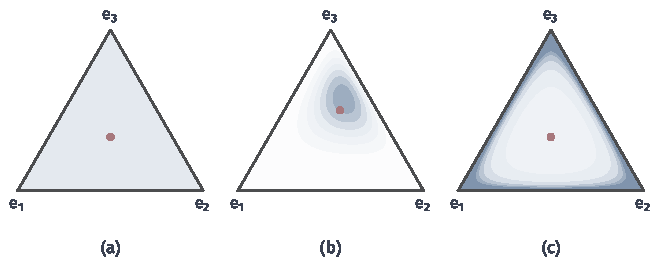
\includegraphics[width=112mm]{figures/07-probability/01-elementary-probability/matplotlib/mvd-dirichlet-density/figure.pdf}
  \caption{Dirichlet密度画在等边三角形上，顶点$\bm{e}_i$对应$p_i=1$；颜色由白到蓝表示密度由小到大，各图色阶分别设定。(a)$\bm{\alpha}=(1,1,1)$，密度恒为$2$。(b)$\bm{\alpha}=(2,3,5)$。(c)$\bm{\alpha}=(0.5,0.5,0.5)$，密度向三条边增大（颜色在$3$处截断）。红点是均值$\bm{\alpha}/\alpha_0$。}
  \label{fig:mvd-dirichlet-density}
\end{BookInlineFigure}

$\bm{\alpha}=(1,1,1)^{\top}$时密度恒为$\Gamma(3)=2$，是$T_2$上的均匀分布：三角形$T_2$的面积是$1/2$。$\alpha_i$都大于$1$时，密度在内部有唯一的峰，在边界上趋于$0$，图~\ref{fig:mvd-dirichlet-density}(b)。

\subsection{Gamma归一化}
\label{sec:mvd-gamma-normalization}

比例最自然的来源是“各部分的量除以总量”。设三种成分的量相互独立，各自是正的随机变量，把它们除以总量，就得到一个随机比例。量取Gamma分布时，比例恰好是Dirichlet分布。

\begin{theorem}[Gamma归一化]
\label{thm:mvd-gamma-normalization}
设随机变量$G_i\sim\operatorname{Gamma}(\alpha_i,\beta)$，$i=1,\ldots,d$，相互独立，速率$\beta>0$相同。令$T=G_1+\cdots+G_d$，则
\begin{equation}
 \bm{P}=\Bigl(\frac{G_1}{T},\ldots,\frac{G_d}{T}\Bigr)^{\top}\sim\operatorname{Dir}(\bm{\alpha}) ,
 \label{eq:mvd-gamma-normalization}
\end{equation}
并且$T\sim\operatorname{Gamma}(\alpha_0,\beta)$，$T$与$\bm{P}$相互独立。
\end{theorem}

证明要求出$(T,P_1,\ldots,P_{d-1})$的联合密度，这是一个$d$维到$d$维的可逆换元，在第~\ref{chap:random-variable-transformations}章用总量与比例的变换完成。这里先核对定理中各项的含义。

\paragraph{取值范围与参数}
每个$G_i$以概率$1$为正，所以$T>0$，各$P_i\in(0,1)$，且$P_1+\cdots+P_d=1$：$\bm{P}$确实落在单纯形内部。第$i$类的形状参数$\alpha_i$原样成为Dirichlet参数的第$i$个分量。形状参数越大，$G_i$越倾向于取大值，第$i$类在总量中占的比例也越大，这与下面算出的均值$\alpha_i/\alpha_0$一致。

\paragraph{共同速率被消去}
速率只是一个共同的单位。若$G\sim\operatorname{Gamma}(\alpha,\beta)$，对$x>0$代换$h=\beta g$，
\[
 \mathbb{P}(\beta G\leq x)=\int_0^{x/\beta}\frac{\beta^{\alpha}g^{\alpha-1}\mathrm{e}^{-\beta g}}{\Gamma(\alpha)}\,\mathrm{d}g=\int_0^{x}\frac{h^{\alpha-1}\mathrm{e}^{-h}}{\Gamma(\alpha)}\,\mathrm{d}h ,
\]
所以$\beta G\sim\operatorname{Gamma}(\alpha,1)$。于是可以写$G_i=H_i/\beta$，$H_i\sim\operatorname{Gamma}(\alpha_i,1)$相互独立，而
\[
 \frac{G_i}{T}=\frac{H_i/\beta}{\sum_jH_j/\beta}=\frac{H_i}{\sum_jH_j} .
\]
比例与$\beta$无关。共同速率只改变各部分的单位，不改变各部分之间的相对大小。

如果各$G_i$的速率不同，速率就不能约去，比例一般不是Dirichlet分布。图~\ref{fig:mvd-gamma-normalization}以$\bm{g}=(1.2,0.6,2.2)$为例：总量为$4$，比例为$(0.3,0.15,0.55)$；所有量同时加倍（相当于速率减半）后总量为$8$，比例不变。

\begin{BookInlineFigure}
  \centering
  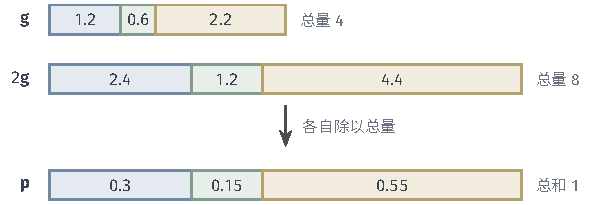
\includegraphics[width=97mm]{figures/07-probability/01-elementary-probability/tikz/mvd-gamma-normalization/figure.pdf}
  \caption{Gamma归一化的一个取值。三种成分的量$\bm{g}=(1.2,0.6,2.2)$（第一行），全部加倍得$2\bm{g}$（第二行）；除以各自的总量$4$与$8$后得到同一个比例向量$\bm{p}=(0.3,0.15,0.55)$（第三行）。}
  \label{fig:mvd-gamma-normalization}
\end{BookInlineFigure}

\paragraph{比例之间为什么相关}
$G_1,\ldots,G_d$相互独立，比例却通过共同的分母联系在一起：某一类的量偏大，总量随之变大，其他各类的比例就被压低。这与多项计数的负相关来源相似，都是“总和固定”在起作用。

定理~\ref{thm:mvd-gamma-normalization}还给出了生成Dirichlet样本的方法：独立地生成$d$个Gamma变量，第$i$个的形状参数为$\alpha_i$、速率为$1$，再各自除以它们的和。下一小节图中的模拟样本就是这样得到的，更多的生成方法在第~\ref{chap:sample-generation}章讨论。

\subsection{均值与协方差}
\label{sec:mvd-dirichlet-moments}

Dirichlet积分把矩的计算变成参数的移位：乘以$p_i$，只是把$\alpha_i$加$1$。对非负整数$r_1,\ldots,r_d$，记$r=\sum_ir_i$，由式~\eqref{eq:mvd-dirichlet-integral}，
\begin{equation}
 \mathbb{E}\Bigl[\prod_{i=1}^{d}P_i^{r_i}\Bigr]=\frac{\Gamma(\alpha_0)}{\Gamma(\alpha_0+r)}\prod_{i=1}^{d}\frac{\Gamma(\alpha_i+r_i)}{\Gamma(\alpha_i)} .
 \label{eq:mvd-dirichlet-moments}
\end{equation}
这里的乘积包括$P_d$，因为$p_d$在被积函数中本来就以幂的形式出现。

\begin{theorem}[Dirichlet的均值与协方差]
\label{thm:mvd-dirichlet-cov}
设$\bm{P}\sim\operatorname{Dir}(\bm{\alpha})$，记$m_i=\alpha_i/\alpha_0$，$\bm{m}=(m_1,\ldots,m_d)^{\top}$。则$\mathbb{E}[\bm{P}]=\bm{m}$，并且
\begin{equation}
 \operatorname{Cov}(\bm{P})=\frac{1}{\alpha_0+1}\bigl(\operatorname{diag}(\bm{m})-\bm{m}\bm{m}^{\top}\bigr) ,
 \label{eq:mvd-dirichlet-cov}
\end{equation}
即$\operatorname{Var}(P_i)=m_i(1-m_i)/(\alpha_0+1)$，$i\neq j$时$\operatorname{Cov}(P_i,P_j)=-m_im_j/(\alpha_0+1)$。
\end{theorem}

\begin{proof}
在式~\eqref{eq:mvd-dirichlet-moments}中用$\Gamma(x+1)=x\Gamma(x)$。只取$r_i=1$，得$\mathbb{E}[P_i]=\alpha_i/\alpha_0$。取$r_i=2$或$r_i=r_j=1$（$i\neq j$），得
\[
 \mathbb{E}[P_i^{2}]=\frac{\alpha_i(\alpha_i+1)}{\alpha_0(\alpha_0+1)},\qquad \mathbb{E}[P_iP_j]=\frac{\alpha_i\alpha_j}{\alpha_0(\alpha_0+1)} .
\]

方差为
\[
 \begin{aligned}
  \operatorname{Var}(P_i)&=\frac{\alpha_i(\alpha_i+1)}{\alpha_0(\alpha_0+1)}-\frac{\alpha_i^{2}}{\alpha_0^{2}}
  =\frac{\alpha_i\bigl[(\alpha_i+1)\alpha_0-\alpha_i(\alpha_0+1)\bigr]}{\alpha_0^{2}(\alpha_0+1)}\\
  &=\frac{\alpha_i(\alpha_0-\alpha_i)}{\alpha_0^{2}(\alpha_0+1)} ,
 \end{aligned}
\]
即$m_i(1-m_i)/(\alpha_0+1)$。协方差为
\[
 \operatorname{Cov}(P_i,P_j)=\frac{\alpha_i\alpha_j}{\alpha_0(\alpha_0+1)}-\frac{\alpha_i\alpha_j}{\alpha_0^{2}}=-\frac{\alpha_i\alpha_j}{\alpha_0^{2}(\alpha_0+1)} .
\]
\end{proof}

用边缘分布核对一下。由式~\eqref{eq:mvd-dirichlet-marginal}，$P_i\sim\operatorname{Beta}(\alpha_i,\alpha_0-\alpha_i)$；按第~\ref{chap:common-distributions}章的Beta公式，均值是$\alpha_i/\alpha_0$，方差是
\[
 \frac{\alpha_i(\alpha_0-\alpha_i)}{\alpha_0^{2}(\alpha_0+1)} ,
\]
与定理一致。也可以用定理~\ref{thm:mvd-gamma-normalization}核对均值：$G_i=TP_i$，而$T$与$\bm{P}$独立，所以
\[
 \frac{\alpha_i}{\beta}=\mathbb{E}[G_i]=\mathbb{E}[T]\,\mathbb{E}[P_i]=\frac{\alpha_0}{\beta}\,\mathbb{E}[P_i] ,
\]
即$\mathbb{E}[P_i]=\alpha_i/\alpha_0$。

取$\bm{\alpha}=(2,3,5)^{\top}$，$\bm{m}=(0.2,0.3,0.5)^{\top}$，$\alpha_0+1=11$。代入式~\eqref{eq:mvd-dirichlet-cov}，
\[
 \operatorname{Cov}(\bm{P})=\frac{1}{11}\begin{bmatrix}0.16&-0.06&-0.10\\-0.06&0.21&-0.15\\-0.10&-0.15&0.25\end{bmatrix}\approx\begin{bmatrix}0.0145&-0.0055&-0.0091\\-0.0055&0.0191&-0.0136\\-0.0091&-0.0136&0.0227\end{bmatrix} .
\]
三个比例两两负相关，每行之和为$0$。

\paragraph{总和约束与奇异协方差}
行和为$0$的原因与多项分布相同：$\operatorname{diag}(\bm{m})-\bm{m}\bm{m}^{\top}$乘以$\bm{1}$得$\bm{m}-\bm{m}=\bm{0}$，对应$\operatorname{Var}(P_1+\cdots+P_d)=0$。各$m_i>0$，所以与多项分布一样，这个矩阵的秩是$d-1$，与单纯形的维数一致。所有比例两两负相关：一个比例变大，其余比例的总和必须变小。

\paragraph{集中程度}
式~\eqref{eq:mvd-dirichlet-cov}把参数分成两部分：方向$\bm{m}=\bm{\alpha}/\alpha_0$决定均值，总和$\alpha_0$决定比例围绕均值的集中程度，协方差与$\alpha_0+1$成反比。$\alpha_0$因此称为\term{集中参数}（concentration parameter）。

固定$\bm{m}=(0.2,0.3,0.5)^{\top}$，让$\alpha_0$取$1,10,100$，$\operatorname{Var}(P_1)=0.16/(\alpha_0+1)$分别是$0.08$、$0.0145$、$0.0016$。图~\ref{fig:mvd-dirichlet-concentration}画出对应的样本。$\alpha_0=1$时各$\alpha_i<1$，样本挤到边和顶点附近，即某一两类占了绝大部分；$\alpha_0=100$时样本紧紧围着$\bm{m}$。

\begin{BookInlineFigure}
  \centering
  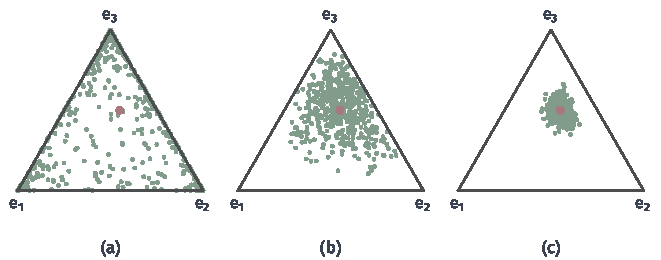
\includegraphics[width=112mm]{figures/07-probability/01-elementary-probability/matplotlib/mvd-dirichlet-concentration/figure.pdf}
  \caption{均值固定为$\bm{m}=(0.2,0.3,0.5)$（红点）、集中参数不同的Dirichlet样本，各$500$个，用Gamma归一化生成。(a)$\alpha_0=1$，种子$51$；(b)$\alpha_0=10$，种子$52$；(c)$\alpha_0=100$，种子$53$。三组样本中$P_1$的样本方差分别约为$0.089$、$0.014$、$0.0016$。}
  \label{fig:mvd-dirichlet-concentration}
\end{BookInlineFigure}


\section{模型比较}
\label{sec:mvd-comparison}

面对一组多元记录，选模型的第一步是看记录的类型：类别计数、实值观测还是组成比例。同一类型中的几个模型，均值甚至协方差可以完全相同，联合规律却不同。本节把前面的结果并排放在一起（表~\ref{tab:mvd-models}），说明哪些特征能区分它们，为什么不能只凭边缘或协方差互相替代。

\begin{BookInlineTable}
  \centering
  \small
  \begin{tabular}{llll}
    \toprule
    模型 & 取值范围 & 协方差矩阵 & 依赖的来源\\
    \midrule
    $\operatorname{Mult}(n,\bm{p})$ & 和为$n$的格点 & $n(\operatorname{diag}\bm{p}-\bm{p}\bm{p}^{\top})$ & 总数固定\\
    多元超几何 & 同上，且$k_i\leq K_i$ & 上式乘$\frac{M-n}{M-1}$ & 总数固定，不放回\\
    $\mathcal{N}(\bm{\mu},\bm{\Sigma})$ & $\bm{\mu}$加$\bm{\Sigma}$的列空间 & $\bm{\Sigma}$ & 共享的高斯分量\\
    多元t & $\mathbb{R}^{d}$ & $\frac{\nu}{\nu-2}\bm{\Sigma}$（$\nu>2$） & 同上，加共同尺度\\
    多元Laplace & $\mathbb{R}^{d}$ & $\bm{\Sigma}$ & 同上，加共同尺度\\
    $\operatorname{Dir}(\bm{\alpha})$ & 单纯形$\Delta_{d-1}$ & $\frac{\operatorname{diag}\bm{m}-\bm{m}\bm{m}^{\top}}{\alpha_0+1}$ & 总和为$1$\\
    \bottomrule
  \end{tabular}
  \caption{本章五个模型及多元超几何分布的取值范围、协方差与依赖来源。多元t与多元Laplace取$\bm{\Sigma}$正定；Dirichlet中$\bm{m}=\bm{\alpha}/\alpha_0$。}
  \label{tab:mvd-models}
\end{BookInlineTable}

\paragraph{计数与比例}
多项分布与多元超几何分布的均值相同，协方差只差因子$(M-n)/(M-1)$；后者还多了上限$k_i\leq K_i$。抽样比例$n/M$小时两者可以互换，抽样比例大时多项分布会高估波动，并给不可能的计数分配概率。

计数比例$\bm{N}/n$与Dirichlet比例更容易混淆。由定理~\ref{thm:mvd-multinomial-moments}，$\bm{N}\sim\operatorname{Mult}(n,\bm{m})$时
\[
 \operatorname{Cov}(\bm{N}/n)=\frac1n\bigl(\operatorname{diag}(\bm{m})-\bm{m}\bm{m}^{\top}\bigr) .
\]
与式~\eqref{eq:mvd-dirichlet-cov}比较，取$n=\alpha_0+1$，两者的均值和协方差完全相同。例如$\bm{m}=(0.2,0.3,0.5)^{\top}$时，$\operatorname{Mult}(11,\bm{m})$的计数比例与$\operatorname{Dir}(2,3,5)$有同样的前两阶矩。

可是两个分布截然不同。$\bm{N}/11$只取$1/11$的整数倍，以正概率恰好等于$0$，例如$\mathbb{P}(N_1=0)=0.8^{11}\approx0.086$；Dirichlet比例在单纯形内部连续取值，$\mathbb{P}(P_1=0)=0$。前两阶矩相同，不足以让一个代替另一个。

\paragraph{实值观测}
多元高斯、多元t与多元Laplace都是椭圆分布：给定$\bm{\mu}$和$\bm{\Sigma}$，三者的等密度面是同一族椭球。区别在于沿椭球向外的衰减，以及有没有共同尺度。为了公平比较，把三者都调到均值为$\bm{0}$、协方差为$\bm{I}_2$：高斯取$\bm{\Sigma}=\bm{I}$，Laplace取$\bm{\Sigma}=\bm{I}$，$\nu=5$的t分布取$\bm{\Sigma}=\tfrac35\bm{I}$，由式~\eqref{eq:mvd-t-cov}，它的协方差也是$\bm{I}$。

第一个差别在边缘的尾部。$\mathbb{P}(\lvert X_1\rvert>3)$在高斯下约为$0.0027$，在Laplace下为$\mathrm{e}^{-3\sqrt2}\approx0.0144$，在t下约为$0.0117$，后两者是高斯的四到五倍，图~\ref{fig:mvd-model-tails}(a)。更远处差别更大：Laplace的尾部按指数衰减，t的尾部按$r^{-5}$衰减，最终比任何指数都慢。

第二个差别在于大值是否一起出现。三者的协方差都是$\bm{I}$，分量两两不相关。若分量独立，$\mathbb{P}(\lvert X_1\rvert>r,\lvert X_2\rvert>r)$应等于$\mathbb{P}(\lvert X_1\rvert>r)^{2}$。对正态尺度混合$\bm{X}=\sqrt{V}\bm{Z}$，先固定$V$再积分，两个概率都可以化为一元积分：记$h(v)=\mathbb{P}(\lvert Z_1\rvert>r/\sqrt v)$，则
\[
 \mathbb{P}(\lvert X_1\rvert>r)=\mathbb{E}[h(V)],\qquad \mathbb{P}(\lvert X_1\rvert>r,\ \lvert X_2\rvert>r)=\mathbb{E}[h(V)^{2}] .
\]

由$\mathbb{E}[h(V)^{2}]\geq(\mathbb{E}[h(V)])^{2}$，比值总不小于$1$，只有$V$为常数时取等号。图~\ref{fig:mvd-model-tails}(b)画出这个比值：高斯恒为$1$；$r=3$时Laplace约为$6.2$，t约为$11.7$。两个分量同时超过$3$的机会，是“假装独立”时估计的六到十几倍。前两节的乘积模型边缘相同、协方差相同，这个比值却恒为$1$。

\begin{BookInlineFigure}
  \centering
  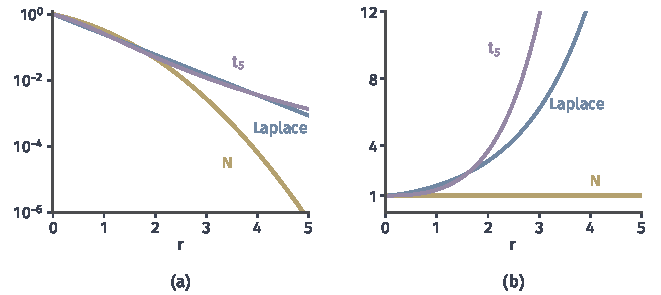
\includegraphics[width=112mm]{figures/07-probability/01-elementary-probability/matplotlib/mvd-model-tails/figure.pdf}
  \caption{均值为$\bm{0}$、协方差为$\bm{I}_2$的三个椭圆模型：高斯（黄）、多元Laplace（蓝）、$\nu=5$的多元t（紫，尺度矩阵$\tfrac35\bm{I}$）。(a)边缘尾概率$\mathbb{P}(\lvert X_1\rvert>r)$，纵轴取对数。(b)联合超越比$\mathbb{P}(\lvert X_1\rvert>r,\lvert X_2\rvert>r)/\mathbb{P}(\lvert X_1\rvert>r)^{2}$，独立时恒为$1$。曲线由对共同尺度的精确密度数值积分得到。}
  \label{fig:mvd-model-tails}
\end{BookInlineFigure}

\paragraph{不相关与独立}
三种实值模型对“不相关能否推出独立”给出不同回答。联合高斯时，零交叉协方差推出独立，定理~\ref{thm:mvd-gaussian-independence}。多元t与多元Laplace中，即使尺度矩阵是对角的，共同尺度也使分量相关于各自的大小，零协方差不推出独立。$(Z,SZ)$说明另一种失效：每个分量都是高斯，但向量不联合高斯，定理同样不适用。

\paragraph{矩与支撑}
矩的存在条件也不同。高斯与Laplace的各阶矩都有限；t分布只有低于$\nu$阶的矩，$\bm{\Sigma}$只在$\nu>2$时通过$\nu/(\nu-2)$与协方差相连。支撑维数则由约束决定：计数与比例都受一条线性约束，住在$d-1$维的格点或单纯形上；退化高斯受$d-r$条线性约束，住在$r$维平面上。凡是有约束的模型，协方差矩阵都奇异，零空间正对应约束方向。

这些比较说明，选择多元模型时要同时核对四件事：取值范围与约束，边缘的尾部，依赖的来源，需要的矩是否存在。只核对均值与协方差，会把本质不同的模型当成可以互换的。


\section{本章小结}
\label{sec:mvd-summary}

本章从试验机制和取值范围出发，写出了五种常见的多元分布，并追问各自的依赖从哪里来。四种构造方式贯穿全章：独立试验的计数，标准高斯向量的仿射像，高斯向量乘以共同的随机尺度，独立Gamma变量除以总量。

计数模型来自独立试验或不放回抽样。多项分布由逐次独立、单次互斥得到协方差$n(\operatorname{diag}\bm{p}-\bm{p}\bm{p}^{\top})$；多元超几何分布的均值相同，协方差多乘有限总体因子$(M-n)/(M-1)$，抽样比例小时可以用多项分布近似。总数固定使协方差矩阵奇异，各类计数两两负相关。

多元高斯定义为$\bm{\mu}+\bm{A}\bm{Z}$的分布，它只由$\bm{\mu}$与$\bm{\Sigma}=\bm{A}\bm{A}^{\top}$决定，在仿射变换下封闭，边缘只需取子块。$\bm{\Sigma}$正定时有满维密度，等密度面是马氏距离的椭球；$\bm{\Sigma}$奇异时分布落在低维平面上。分块后，条件均值是观测的仿射函数，条件协方差是与观测无关的Schur补；残差与观测独立，这一正交分解也给出了高斯样本平均与残差平方和的独立性。零交叉协方差推出独立，只在联合高斯时成立。

多元t与多元Laplace把高斯的固定尺度换成共同的随机尺度：t用$\sqrt{\nu/U}$，尾部按负幂衰减，只有低于$\nu$阶的矩，$\bm{\Sigma}$是尺度矩阵；Laplace用$\sqrt W$，边缘是一元Laplace，各阶矩有限，$\bm{\Sigma}$就是协方差。两者都是椭圆分布，尺度矩阵为对角时分量不相关却不独立，大值倾向于同时出现；改用各分量独立的尺度，得到边缘与协方差相同而联合规律不同的乘积模型。

Dirichlet分布描述单纯形上的随机比例，密度相对于$d-1$个自由坐标给出，参数小于一时在边界附近无界却没有点质量。它可以由同速率独立Gamma变量归一化得到，边缘是Beta分布，均值为$\bm{\alpha}/\alpha_0$，协方差与$\alpha_0+1$成反比，并因总和为$1$而奇异。

本章多次用到“已知输入的分布，求输出的分布”：仿射像的密度、尺度混合的密度、Gamma归一化的联合密度。第~\ref{chap:random-variable-transformations}章把这些具体计算整理成一般的变换方法，补全了本章留给它的换元证明。


\chapter{随机变量的运算与变换}
\label{chap:random-variable-transformations}

掷两枚骰子，我们知道每一对点数的概率都是$1/36$，可真正关心的常常是点数之和、两点之差或较大的那一个。量一块方形木板的边长，测量值有误差，算出的面积也就有误差，面积的误差分布与边长的不同。两段相互独立的等待时间，它们的比值落在$1$附近的可能性有多大？这些问题的共同形式是：输入变量的规律已经知道，输出由一个确定的公式算出，求输出的分布。

前几章的工具已经能回答其中一部分。第~\ref{chap:random-variable-moments}章说，求$g(X)$的期望不必先求它的分布；第~\ref{chap:random-vectors}章说，和的方差可以由各自的方差与协方差算出。但“和超过$10$的概率”“比值的尾部有多重”这类问题需要完整的输出分布，少数几个数值特征不够。

本章只用一条规则：输出落在某个范围，等价于输入落在这个范围的原像里。离散时把原像中的概率质量加起来，连续时在原像上积分密度。规则本身很简单，难处在把原像写清楚，并在需要密度时把积分换到输出的坐标上。换坐标时，单调映射要注意不等号的方向，非单调映射要把几个逆像的贡献都加上，多元映射要用行列式记录体积的伸缩，降维映射要先补足坐标再积掉多余的部分。

我们先在第一节建立这条规则，并说明独立性在什么条件下能保持、没有独立性时边缘分布为什么不够。第二、三节分别处理一元和多元的确定映射。后四节把同一套方法用到和、差、乘积、比值和排序上，每种运算都会增加自己的条件：卷积需要独立，乘积要另计零点的质量，比值要求分母不取零，排序遇到同值要换一种计数。全章反复使用两个小例子：两枚骰子，以及单位正方形上的两个独立均匀变量。

\section{运算后的分布}
\label{sec:rvt-output-distribution}

两枚均匀骰子的点数记为$X_1,X_2$，三十六种结果等可能。点数之和$S=X_1+X_2$取$2$到$12$之间的整数，它取各个值的概率是多少？输出的规律要从输入的规律算出来，这一节先把这件事的一般做法说清楚。

\paragraph{把目标事件写回输入}
事件“$S=7$”发生，当且仅当点数对落在
\[
 \{(1,6),(2,5),(3,4),(4,3),(5,2),(6,1)\}
\]
之中。这六个结果各有概率$1/36$，于是$\mathbb{P}(S=7)=6/36$。我们没有直接研究$S$，而是把关于$S$的事件翻译成关于$(X_1,X_2)$的事件，再用已知的联合规律计算。

图~\ref{fig:rvt-dice-sum-grid}(a)把三十六个结果画成方格，同一条斜线上的格子和相同。$S=s$对应的格子数从$s=2$的$1$个增加到$s=7$的$6$个，再减到$s=12$的$1$个，于是
\[
 \mathbb{P}(S=s)=\frac{6-\lvert s-7\rvert}{36},\qquad s=2,3,\ldots,12 .
\]
十一个概率之和是$(1+2+\cdots+6+5+\cdots+1)/36=1$。

\begin{BookInlineFigure}
  \centering
  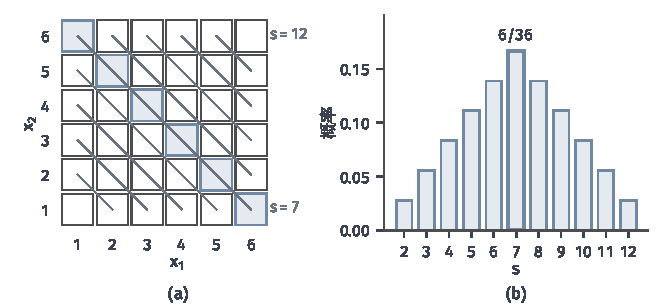
\includegraphics[width=112mm]{figures/07-probability/01-elementary-probability/matplotlib/rvt-dice-sum-grid/figure.pdf}
  \caption{两枚骰子之和。(a)三十六个等可能结果，灰线连接和相同的格子，蓝色格子是事件$S=7$的原像。(b)$S$的概率质量，第$s$根柱的高度等于(a)中第$s$条斜线上的格子数除以$36$。}
  \label{fig:rvt-dice-sum-grid}
\end{BookInlineFigure}

\paragraph{原像规则}
设$X$是一个随机变量或随机向量，$g$是定义在其取值范围上的确定函数，$Y=g(X)$。对输出的一个取值集合$B$，输入的\term{原像}（preimage）是
\[
 g^{-1}(B)=\{x:\ g(x)\in B\} .
\]
这里$g^{-1}(B)$只是一个集合的记号，$g$不必可逆。事件“$Y\in B$”与“$X\in g^{-1}(B)$”由同样的试验结果组成，所以它们的概率相等：
\begin{equation}
 \mathbb{P}(Y\in B)=\mathbb{P}\bigl(X\in g^{-1}(B)\bigr) .
 \label{eq:rvt-preimage-rule}
\end{equation}
多个输入的情形完全一样，只是把$X$换成随机向量$(X_1,\ldots,X_n)$，右端用联合分布计算。

式~\eqref{eq:rvt-preimage-rule}在两种模型下分别落成求和与积分。$X$离散时，取$B=\{y\}$，原像是所有被送到$y$的输入，于是
\begin{equation}
 p_Y(y)=\sum_{x:\ g(x)=y}p_X(x) .
 \label{eq:rvt-discrete-pushforward}
\end{equation}
$X$有密度$f_X$时，取$B=(-\infty,y]$，得到输出的分布函数
\begin{equation}
 F_Y(y)=\int_{\{x:\ g(x)\leq y\}}f_X(x)\,\mathrm{d}x .
 \label{eq:rvt-cdf-method}
\end{equation}
这里的集合$B$取区间、区域等前几章能计算概率的集合；哪些集合都能这样处理，在第~\ref{chap:probability-spaces}章统一说明。

\paragraph{搬运质量的图景}
把概率看成总量为$1$的质量，式~\eqref{eq:rvt-discrete-pushforward}说的是：每个输入格子把自己的质量搬到$g$指定的输出位置，落在同一位置的质量相加。图~\ref{fig:rvt-dice-sum-grid}中，一条斜线上的六个格子把质量都搬到$7$，所以$7$处堆得最高。

这个图景在连续情形要补一句。密度是单位长度上的质量，质量被搬走时如果所占的长度被拉长或压短，单位长度上的质量就要相应变小或变大。式~\eqref{eq:rvt-cdf-method}只算总质量，不受这一点影响；从它求密度时，伸缩就会出现在公式里，这是下一节的主题。

\paragraph{分布与函数期望}
第~\ref{chap:random-variable-moments}章计算$\mathbb{E}[g(X)]$时直接对$X$的分布加权，不先求$g(X)$的分布。骰子的例子里
\[
 \mathbb{E}[S]=\sum_{x_1=1}^{6}\sum_{x_2=1}^{6}\frac{x_1+x_2}{36}=7 .
\]
两种算法给出同一个结果。按式~\eqref{eq:rvt-discrete-pushforward}，把输入按$g(x)$的值分组，组内的$g(x)$都等于同一个$y$：
\[
 \sum_{x}g(x)\,p_X(x)=\sum_{y}\ y\sum_{x:\ g(x)=y}p_X(x)=\sum_{y}y\,p_Y(y) .
\]
分组只是改变了加法的次序；无穷多项时这一步要求级数绝对收敛，这正是期望存在的条件。

两件事回答的问题不同。一个期望只是分布的一个数值，知道$\mathbb{E}[S]=7$不能推出$\mathbb{P}(S\geq10)$。反过来，输出分布确定了$Y$的每一个函数的期望，例如
\[
 \mathbb{P}(S\geq10)=\mathbb{E}\bigl[\mathbf{1}_{\{S\geq10\}}\bigr]=\frac{3+2+1}{36}=\frac16 .
\]
要回答关于$Y$的所有概率问题，就需要求出$Y$的分布；只要一两个平均值时，直接按第~\ref{chap:random-variable-moments}章计算更省事。

\paragraph{独立性的保持}
把四枚骰子分成两组，前两枚的点数和$S=X_1+X_2$与后两枚的较大值$M=\max(X_3,X_4)$是否独立？直觉上是：两组骰子互不影响，各自算出的量也互不影响。下面的定理说明这个直觉在什么条件下成立。

称随机向量$\bm{U}=(X_1,\ldots,X_k)$与$\bm{W}=(X_{k+1},\ldots,X_n)$相互独立，是指它们的联合概率质量（或联合密度）等于两组各自联合质量（或密度）的乘积。$X_1,\ldots,X_n$相互独立时，第~\ref{chap:random-vectors}章的乘积分解按组归并，就得到这一点。

\begin{theorem}[分组变换保持独立]
\label{thm:rvt-group-independence}
设$\bm{U}$与$\bm{W}$相互独立，$g$、$h$是确定的函数。则对能计算概率的取值集合$A$、$B$，
\begin{equation}
 \mathbb{P}\bigl(g(\bm{U})\in A,\ h(\bm{W})\in B\bigr)=\mathbb{P}\bigl(g(\bm{U})\in A\bigr)\,\mathbb{P}\bigl(h(\bm{W})\in B\bigr) .
 \label{eq:rvt-group-independence}
\end{equation}
即$g(\bm{U})$与$h(\bm{W})$相互独立。
\end{theorem}

\begin{proof}
记$A'=g^{-1}(A)$，$B'=h^{-1}(B)$。由原像规则，左端的事件就是$\bm{U}\in A'$且$\bm{W}\in B'$。

离散情形，联合质量写成$p_{\bm{U}}(\bm{u})\,p_{\bm{W}}(\bm{w})$，对$\bm{u}\in A'$、$\bm{w}\in B'$求和。二重和中的每一项是两个因子的乘积，第一个只依赖$\bm{u}$，第二个只依赖$\bm{w}$，所以
\[
 \sum_{\bm{u}\in A'}\sum_{\bm{w}\in B'}p_{\bm{U}}(\bm{u})\,p_{\bm{W}}(\bm{w})=\Bigl(\sum_{\bm{u}\in A'}p_{\bm{U}}(\bm{u})\Bigr)\Bigl(\sum_{\bm{w}\in B'}p_{\bm{W}}(\bm{w})\Bigr) .
\]
右端两个因子分别是$\mathbb{P}(\bm{U}\in A')$与$\mathbb{P}(\bm{W}\in B')$，再用一次原像规则，就是式~\eqref{eq:rvt-group-independence}的右端。

有密度时把求和换成积分。积分区域是乘积集合$A'\times B'$，被积函数是$f_{\bm{U}}(\bm{u})f_{\bm{W}}(\bm{w})$，按累次积分先对$\bm{w}$、后对$\bm{u}$积分，内层积分与$\bm{u}$无关，可以提到外面，得到同样的乘积。
\end{proof}

证明只用到一件事：两组输入的联合规律可以分解，而$g$只读第一组、$h$只读第二组，于是两个原像分别落在乘积的两个因子里。所以$S$与$M$独立。

条件中的“分组”不能省。$S=X_1+X_2$与$D=X_1-X_2$都只由前两枚骰子算出，但它们读的是同一组输入。$S=2$迫使两枚骰子都是$1$，于是$D=0$；所以
\[
 \mathbb{P}(S=2,\ D=1)=0,\qquad \mathbb{P}(S=2)\,\mathbb{P}(D=1)=\frac{1}{36}\cdot\frac{5}{36}>0 ,
\]
$S$与$D$不独立。

\paragraph{边缘分布的不足}
没有独立结构时，只知道每个输入各自的分布，输出的分布通常还不确定。最小的例子是两个只取$0,1$的变量$X,Y$，各自都满足$\mathbb{P}(X=1)=\mathbb{P}(Y=1)=1/2$。下面三种联合规律都与这两个边缘相容：
\begin{itemize}
 \item 独立：四个格子各有$1/4$，和$X+Y$取$0,1,2$的概率是$1/4,1/2,1/4$；
 \item 完全一致，$Y=X$：质量只在$(0,0)$与$(1,1)$，和取$0,2$各$1/2$；
 \item 完全相反，$Y=1-X$：质量只在$(0,1)$与$(1,0)$，和恒等于$1$。
\end{itemize}

图~\ref{fig:rvt-same-marginals}把三张概率表和对应的和画在一起。三张表的行和与列和都是$(1/2,1/2)$，和的期望都是$1$，可是和的分布从“三点”变成“两点”，再变成一个确定的数。

\begin{BookInlineFigure}
  \centering
  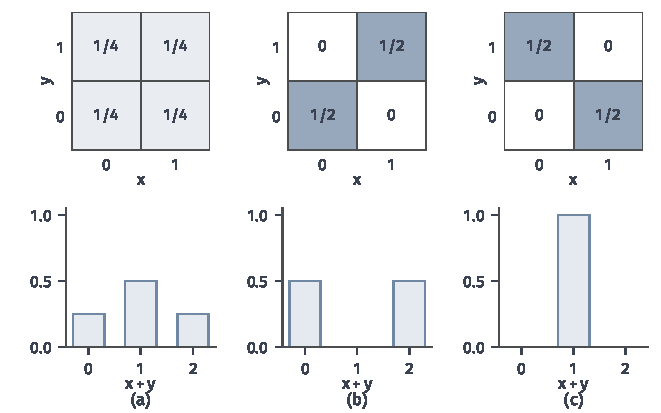
\includegraphics[width=112mm]{figures/07-probability/01-elementary-probability/matplotlib/rvt-same-marginals/figure.pdf}
  \caption{相同边缘、不同联合规律下的和。上排是$(X,Y)$的三张概率表，格中数字与蓝色深浅表示概率，三张表的行和与列和都是$1/2$。下排是对应的$X+Y$的概率质量：(a)独立，(b)$Y=X$，(c)$Y=1-X$。}
  \label{fig:rvt-same-marginals}
\end{BookInlineFigure}

原因在原像。事件$X+Y=1$的原像是两个对角格子$\{(0,1),(1,0)\}$，边缘分布只规定行和与列和，对角格子上的质量可以在$0$到$1/2$之间任意选。所以计算输出分布时要先确认用的是联合规律；只有在独立时，联合规律才能由边缘相乘得到。后面讲和、乘积、比值时都会把一般公式与独立情形分开写。


\section{一元变换}
\label{sec:rvt-univariate}

设$X$有密度$f_X$，$g$是实轴上的函数，$Y=g(X)$。$Y$有没有密度？有的话怎样从$f_X$算出来？离散的情形已经由式~\eqref{eq:rvt-discrete-pushforward}解决，难点在连续的情形。

\paragraph{先求分布函数}
最稳妥的办法分两步。第一步取阈值事件$\{Y\leq y\}$，写出它的原像，用式~\eqref{eq:rvt-cdf-method}求出$F_Y(y)$；这一步对任何$g$都适用。第二步在$F_Y$可导的地方求导得到密度，这一步需要条件，后面两小节说明。这种做法称为\term{分布函数法}（distribution function method）。

以$X\sim\operatorname{Unif}(0,1)$、$Y=X^2$为例。$Y$取值于$(0,1)$。对$0<y<1$，$X^2\leq y$与$X\leq\sqrt{y}$等价，因为$X$只取正值，于是
\[
 F_Y(y)=\mathbb{P}(X\leq\sqrt{y})=\sqrt{y} .
\]
$y\leq0$时$F_Y(y)=0$，$y\geq1$时$F_Y(y)=1$。在$(0,1)$内求导，得到
\[
 f_Y(y)=\frac{1}{2\sqrt{y}},\qquad 0<y<1 .
\]

$X$的密度在$(0,1)$上处处是$1$，$Y$的密度却在$0$附近无界。原因是平方把$0$附近的数压得更挤：$X\in(0,0.1)$的概率是$0.1$，被送进长度只有$0.01$的区间$(0,0.01)$，单位长度上的质量变成$10$倍。

图~\ref{fig:rvt-preimage-cdf}画出阈值事件的原像。在$(0,1)$上，$X^2\leq y$的原像是一段从$0$开始的区间；如果$X$也取负值，比如$X\sim\operatorname{Unif}(-1,2)$，原像就变成$[-\sqrt{y},\sqrt{y}]$与支撑的交，两个端点同时移动。前者是单调变换，后者是多分支变换，分别在下面两小节处理。

\begin{BookInlineFigure}
  \centering
  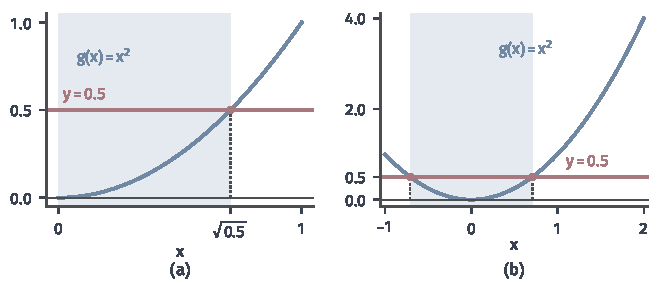
\includegraphics[width=112mm]{figures/07-probability/01-elementary-probability/matplotlib/rvt-preimage-cdf/figure.pdf}
  \caption{阈值事件的原像。蓝线是$g(x)=x^2$，红色水平线是阈值$y=0.5$，横轴上的浅蓝区间是$\{x:\ x^2\leq0.5\}$与$X$的支撑之交。(a)$X$取值于$(0,1)$，原像是$(0,\sqrt{0.5}\,]$；(b)$X$取值于$(-1,2)$，原像是$[-\sqrt{0.5},\sqrt{0.5}\,]$，左右两端都随$y$移动。}
  \label{fig:rvt-preimage-cdf}
\end{BookInlineFigure}

\subsection{单调变换}
\label{sec:rvt-monotone}

上面的计算每次都要从分布函数重新开始。对单调的$g$，这两步可以合成一个公式，并且看清密度为什么要乘以一个伸缩因子。

\paragraph{阈值事件的翻译}
设$g$在$X$的取值区间上严格递增，反函数为$h$。$g(X)\leq y$与$X\leq h(y)$等价，于是
\[
 F_Y(y)=F_X\bigl(h(y)\bigr) .
\]
$g$严格递减时，不等号要翻转：$g(X)\leq y$与$X\geq h(y)$等价。$X$有密度，单点的概率为零，于是
\[
 F_Y(y)=\mathbb{P}\bigl(X\geq h(y)\bigr)=1-F_X\bigl(h(y)\bigr) .
\]

\paragraph{长度的伸缩}
求导之前先看密度应当变成什么。$X$落在$[x,x+\Delta x]$的概率约为$f_X(x)\Delta x$。$g$把这段区间送到以$g(x)$为一端、长度约$\lvert g'(x)\rvert\Delta x$的区间，概率不变，长度乘了$\lvert g'(x)\rvert$，所以单位长度上的质量要除以$\lvert g'(x)\rvert$。这就得到下面的公式，导数取绝对值，因为长度总是正的。

\begin{theorem}[单调变换的密度]
\label{thm:rvt-monotone-density}
设$X$的密度$f_X$在开区间$I$之外为零（$I$可以无界），$g$在$I$上严格单调、连续可导，且对所有$x\in I$有$g'(x)\neq0$。记$J=g(I)$，$h:J\to I$为$g$的反函数。则$Y=g(X)$有密度
\begin{equation}
 f_Y(y)=
 \begin{cases}
  f_X\bigl(h(y)\bigr)\,\lvert h'(y)\rvert, & y\in J,\\
  0, & y\notin J .
 \end{cases}
 \label{eq:rvt-monotone-density}
\end{equation}
其中$h'(y)=1/g'(h(y))$。
\end{theorem}

\begin{proof}
由一元反函数的求导法则，$h$在开区间$J$上连续可导，且$h'(y)=1/g'(h(y))$。只需证明对$J$内任意闭区间$[c,d]$，$\mathbb{P}(c\leq Y\leq d)$等于式~\eqref{eq:rvt-monotone-density}在$[c,d]$上的积分；区间概率确定了分布函数，也就确定了分布。

先设$g$递增，此时$h$也递增，$h'>0$。原像规则给出
\[
 \mathbb{P}(c\leq Y\leq d)=\mathbb{P}\bigl(h(c)\leq X\leq h(d)\bigr)=\int_{h(c)}^{h(d)}f_X(x)\,\mathrm{d}x .
\]
作换元$x=h(y)$，$\mathrm{d}x=h'(y)\,\mathrm{d}y$，积分限$h(c),h(d)$对应$c,d$，得到
\[
 \int_{h(c)}^{h(d)}f_X(x)\,\mathrm{d}x=\int_c^d f_X\bigl(h(y)\bigr)\,h'(y)\,\mathrm{d}y .
\]
这里$h'=\lvert h'\rvert$，就是要证的等式。

再设$g$递减，此时$h$递减，$h'<0$，原像变成$[h(d),h(c)]$。同样的换元给出
\[
 \int_{h(d)}^{h(c)}f_X(x)\,\mathrm{d}x=\int_d^c f_X\bigl(h(y)\bigr)\,h'(y)\,\mathrm{d}y=\int_c^d f_X\bigl(h(y)\bigr)\bigl(-h'(y)\bigr)\,\mathrm{d}y .
\]
交换积分限产生的负号与$h'<0$抵消，被积函数仍是$f_X(h(y))\lvert h'(y)\rvert$。

$J$外的区间原像为空，概率为零。$I$无界或$f_X$在端点附近无界时，上面的积分是反常积分，先在内部的闭区间上换元，再令端点趋于边界即可。
\end{proof}

换元积分的依据见\BookChapterRef{chap:univariate-integration}{卷一第7章“一元函数的积分”}。证明中递减情形的处理正好对应前面的两件事：阈值事件的不等号翻转，表现为积分限交换；长度为正，表现为导数取绝对值。

条件各有作用。严格单调保证每个$y$只有一个逆像，原像是一段区间。$g'\neq0$保证小区间不会被压成一个点；它一旦在某段区间上失效，就会产生原子。连续可导是换元公式所需的光滑性。最后，$J=g(I)$交代了输出的支撑，式~\eqref{eq:rvt-monotone-density}在$J$外必须补成零。

\paragraph{线性变换}
$Y=aX+b$，$a\neq0$。反函数$h(y)=(y-b)/a$，$\lvert h'(y)\rvert=1/\lvert a\rvert$，于是
\begin{equation}
 f_Y(y)=\frac{1}{\lvert a\rvert}\,f_X\Bigl(\frac{y-b}{a}\Bigr) .
 \label{eq:rvt-linear-density}
\end{equation}
$a>0$时密度的形状被横向拉伸$a$倍、纵向压低$a$倍，再平移$b$；$a<0$时还要左右翻转。

两个具体情形。$X\sim\mathcal{N}(\mu,\sigma^{2})$时，代入密度并整理指数，得到
\[
 f_Y(y)=\frac{1}{\sqrt{2\pi}\,\lvert a\rvert\sigma}\exp\Bigl(-\frac{(y-a\mu-b)^2}{2a^2\sigma^2}\Bigr),
\]
即$Y\sim\mathcal{N}(a\mu+b,a^2\sigma^2)$，高斯族在仿射变换下保持不变。$X\sim\operatorname{Unif}(0,1)$、$Y=3-2X$时，$a=-2$，$Y$的支撑是$(1,3)$，密度为$1/2$；支撑的端点由$I=(0,1)$的端点经$g$映过去，次序也翻转了。

\paragraph{指数变换}
设$X\sim\mathcal{N}(\mu,\sigma^{2})$，$Y=\mathrm{e}^{X}$。$g(x)=\mathrm{e}^{x}$把$I=\mathbb{R}$映到$J=(0,\infty)$，反函数$h(y)=\ln y$，$h'(y)=1/y$。代入式~\eqref{eq:rvt-monotone-density}，得到
\begin{equation}
 f_Y(y)=\frac{1}{y\,\sigma\sqrt{2\pi}}\exp\Bigl(-\frac{(\ln y-\mu)^2}{2\sigma^2}\Bigr),\qquad y>0 .
 \label{eq:rvt-lognormal}
\end{equation}
这个分布称为\term{对数正态分布}（log-normal distribution）：取对数之后服从高斯分布。输出只取正值，这来自$g$的值域，而不是来自$X$的密度。

图~\ref{fig:rvt-lognormal-strip}取$\mu=0$、$\sigma=1$，把$X$的一条小区间$[0.5,0.7]$和它的像$[\mathrm{e}^{0.5},\mathrm{e}^{0.7}]\approx[1.649,2.014]$画在一起。两块浅蓝面积都等于$\Phi(0.7)-\Phi(0.5)\approx0.0666$，其中$\Phi$是标准高斯分布函数。像区间的长度约$0.365$，比原来的$0.2$长，所以那里的密度相应变低。

\begin{BookInlineFigure}
  \centering
  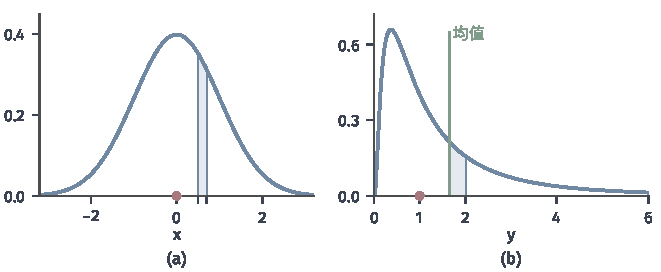
\includegraphics[width=112mm]{figures/07-probability/01-elementary-probability/matplotlib/rvt-lognormal-strip/figure.pdf}
  \caption{指数变换下质量守恒、长度伸缩。(a)$X\sim\mathcal{N}(0,1)$的密度，浅蓝区间为$[0.5,0.7]$；(b)$Y=\mathrm{e}^{X}$的对数正态密度，浅蓝区间为像$[\mathrm{e}^{0.5},\mathrm{e}^{0.7}]$，两块面积都约为$0.0666$。红点标出中位数：$X$的中位数$0$对应$Y$的中位数$1$；绿色竖线是$Y$的均值$\mathrm{e}^{1/2}$。}
  \label{fig:rvt-lognormal-strip}
\end{BookInlineFigure}

单调变换保持分位数：$X$的中位数是$0$，$\mathrm{e}^{X}\leq\mathrm{e}^{0}$与$X\leq0$等价，所以$Y$的中位数是$\mathrm{e}^{0}=1$。均值却不这样传递。按第~\ref{chap:random-variable-moments}章的函数期望，对指数配方，得到
\[
 \mathbb{E}[\mathrm{e}^{X}]=\int_{\mathbb{R}}\frac{\mathrm{e}^{x}}{\sqrt{2\pi}\sigma}\mathrm{e}^{-(x-\mu)^2/(2\sigma^2)}\,\mathrm{d}x=\mathrm{e}^{\mu+\sigma^2/2} .
\]
$\mu=0$、$\sigma=1$时均值约为$1.649$，大于$\mathrm{e}^{\mathbb{E}[X]}=1$。这与Jensen不等式一致：$\mathrm{e}^{x}$是凸函数，先平均再变换小于先变换再平均。

\paragraph{递减的情形}
设$X\sim\operatorname{Exp}(\lambda)$，$Y=\mathrm{e}^{-X}$。$g$把$(0,\infty)$递减地映到$(0,1)$，反函数$h(y)=-\ln y$。先用阈值事件：对$0<y<1$，$\mathrm{e}^{-X}\leq y$与$X\geq-\ln y$等价，不等号翻转了，于是
\[
 F_Y(y)=\mathbb{P}(X\geq-\ln y)=\mathrm{e}^{-\lambda(-\ln y)}=y^{\lambda} .
\]

再用式~\eqref{eq:rvt-monotone-density}核对。$h'(y)=-1/y$，取绝对值得$1/y$；密度在逆像处的值是
\[
 f_X\bigl(h(y)\bigr)=\lambda\mathrm{e}^{\lambda\ln y}=\lambda y^{\lambda} .
\]
两者相乘，得到
\[
 f_Y(y)=\lambda y^{\lambda}\cdot\frac{1}{y}=\lambda y^{\lambda-1},\qquad 0<y<1 ,
\]
正是$F_Y(y)=y^{\lambda}$的导数。$\lambda=1$时$Y\sim\operatorname{Unif}(0,1)$；反过来读，$U\sim\operatorname{Unif}(0,1)$时$-\ln U\sim\operatorname{Exp}(1)$。

递减情形有两处容易出错，图~\ref{fig:rvt-decreasing-map}取$\lambda=2$画出正确结果。若忘了翻转不等号，会写出$F_Y(y)=1-y^{2}$，它随$y$递减，不可能是分布函数。若忘了绝对值，会得到“密度”$-2y$，它是负的。两个检查——分布函数递增、密度非负——可以随手做。

\begin{BookInlineFigure}
  \centering
  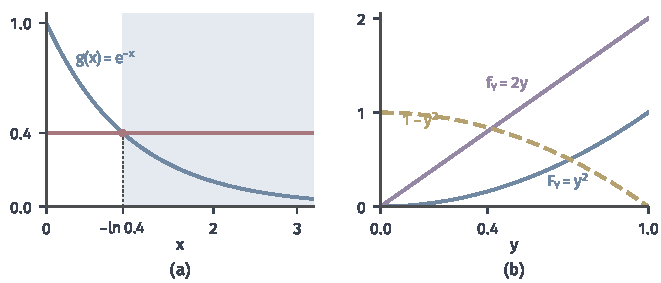
\includegraphics[width=112mm]{figures/07-probability/01-elementary-probability/matplotlib/rvt-decreasing-map/figure.pdf}
  \caption{递减变换$Y=\mathrm{e}^{-X}$，$X\sim\operatorname{Exp}(2)$。(a)蓝线为$g(x)=\mathrm{e}^{-x}$，红线为阈值$y=0.4$，事件$Y\leq0.4$的原像是横轴上的右侧区间$[-\ln0.4,\infty)$（浅蓝）。(b)$Y$的分布函数$y^{2}$（蓝）与密度$2y$（紫），黄色虚线是不翻转不等号得到的$1-y^{2}$，它不是分布函数。}
  \label{fig:rvt-decreasing-map}
\end{BookInlineFigure}

\paragraph{非退化条件失效}
条件$g'\neq0$去掉会怎样，要分两种情况看。第一种是$g$在一段区间上为常数。取$X\sim\operatorname{Unif}(0,2)$，$Y=\min(X,1)$。$X\in[1,2)$的全部质量都被送到点$1$，于是
\[
 \mathbb{P}(Y=1)=\mathbb{P}(X\geq1)=\frac12 .
\]
$Y$的分布函数在$1$处跳跃$1/2$，没有密度。若只在$(0,1)$上套用式~\eqref{eq:rvt-monotone-density}，得到的函数是$1/2$，总积分只有$1/2$，另一半质量丢在了原子上。

第二种是$g'$只在孤立点为零。取$X\sim\operatorname{Unif}(-1,1)$，$Y=X^3$，$g'(0)=0$。去掉单点$0$，把$I$分成$(-1,0)$与$(0,1)$，每段上定理的条件都成立；单点的概率为零，不影响结果。两段的反函数都是$h(y)=y^{1/3}$，在$y\neq0$处$\lvert h'(y)\rvert=\tfrac13\lvert y\rvert^{-2/3}$，于是
\[
 f_Y(y)=\frac12\cdot\frac{1}{3\lvert y\rvert^{2/3}}=\frac{1}{6\lvert y\rvert^{2/3}},\qquad 0<\lvert y\rvert<1 .
\]
它在$0$附近无界，但可积，总积分为$2\cdot\tfrac16\cdot3=1$。

图~\ref{fig:rvt-flat-atom}对比两种情况。导数在一段区间上为零，会把正长度的区间压成一个点，产生原子；只在一个点上为零，压缩的是零概率的点，密度变得无界，但仍然存在。

\begin{BookInlineFigure}
  \centering
  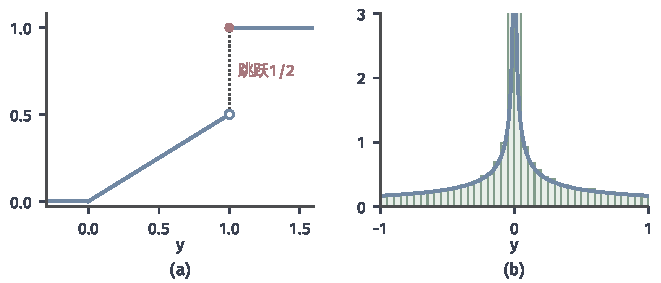
\includegraphics[width=112mm]{figures/07-probability/01-elementary-probability/matplotlib/rvt-flat-atom/figure.pdf}
  \caption{导数为零的两种后果。(a)$Y=\min(X,1)$，$X\sim\operatorname{Unif}(0,2)$，分布函数（蓝）在$y=1$处跳跃$1/2$，红点表示该原子。(b)$Y=X^3$，$X\sim\operatorname{Unif}(-1,1)$，密度$\tfrac16\lvert y\rvert^{-2/3}$（蓝）在$0$附近无界，浅绿直方图是$20000$个模拟样本（种子$7$）。}
  \label{fig:rvt-flat-atom}
\end{BookInlineFigure}

\subsection{多分支变换}
\label{sec:rvt-branches}

$g$不单调时，一个$y$可以有几个逆像。图~\ref{fig:rvt-preimage-cdf}(b)中，$X\sim\operatorname{Unif}(-1,2)$，$y=0.5$有两个逆像$\pm\sqrt{0.5}$，而$y=2$只有一个逆像$\sqrt2$，因为$-\sqrt2$在支撑之外。要把每个逆像附近的质量都收集起来。

\paragraph{分支相加}
做法是把输入区域切成几段，每段上$g$单调，在每段上用单调变换的公式，再把各段的贡献相加。用质量的图景说，输出$y$附近的质量来自几处输入，每处按自己的伸缩比例换算后叠在一起。

\begin{theorem}[多分支变换的密度]
\label{thm:rvt-branch-density}
设$X$的密度在$I_1\cup\cdots\cup I_m$之外为零，其中$I_1,\ldots,I_m$是互不相交的开区间（除去有限个点后覆盖$X$的取值范围）。设$g$在每个$I_k$上满足定理~\ref{thm:rvt-monotone-density}的条件，$h_k$是$g$在$I_k$上的反函数，定义在$J_k=g(I_k)$上。则$Y=g(X)$有密度
\begin{equation}
 f_Y(y)=\sum_{k:\ y\in J_k}f_X\bigl(h_k(y)\bigr)\,\lvert h_k'(y)\rvert .
 \label{eq:rvt-branch-density}
\end{equation}
\end{theorem}

\begin{proof}
对任意区间$[c,d]$，事件$c\leq Y\leq d$按$X$落在哪一段分解为互不相交的事件之并，剩下的有限个点概率为零：
\[
 \mathbb{P}(c\leq Y\leq d)=\sum_{k=1}^{m}\mathbb{P}\bigl(X\in I_k,\ c\leq g(X)\leq d\bigr) .
\]
第$k$项等于$f_X\mathbf{1}_{I_k}$在$I_k\cap g^{-1}([c,d])$上的积分。定理~\ref{thm:rvt-monotone-density}的证明只用到换元积分，没有用到总质量为$1$，所以对$f_X\mathbf{1}_{I_k}$同样成立，第$k$项等于$f_X(h_k(y))\lvert h_k'(y)\rvert$在$[c,d]\cap J_k$上的积分。对$k$求和，得到式~\eqref{eq:rvt-branch-density}在$[c,d]$上的积分。
\end{proof}

\paragraph{平方变换}
设$Z\sim\mathcal{N}(0,1)$，$Y=Z^2$。两段$I_1=(-\infty,0)$、$I_2=(0,\infty)$都被映到$(0,\infty)$，反函数$h_{1,2}(y)=\mp\sqrt{y}$，$\lvert h_k'(y)\rvert=1/(2\sqrt{y})$。记标准高斯密度为$\varphi(z)=\mathrm{e}^{-z^2/2}/\sqrt{2\pi}$，它是偶函数，两项相等，于是
\begin{equation}
 f_Y(y)=2\cdot\varphi(\sqrt{y})\cdot\frac{1}{2\sqrt{y}}=\frac{1}{\sqrt{2\pi}}\,y^{-1/2}\mathrm{e}^{-y/2},\qquad y>0 .
 \label{eq:rvt-chi2-one}
\end{equation}
与第~\ref{chap:common-distributions}章的Gamma密度比较，这正是$\operatorname{Gamma}(1/2,1/2)$，即自由度为$1$的$\chi^2$分布：标准高斯的平方服从$\chi^2_1$。只取$h_2(y)=\sqrt{y}$一支，得到的函数总积分为$1/2$，漏掉了$Z<0$的一半。

支撑不对称时，各段的像可以不同。$X\sim\operatorname{Unif}(-1,2)$，密度$1/3$，$Y=X^2$取值于$(0,4)$。$I_1=(-1,0)$映到$J_1=(0,1)$，$I_2=(0,2)$映到$J_2=(0,4)$。$0<y<1$时两支都有贡献，$1<y<4$时只有右支，于是
\[
 f_Y(y)=
 \begin{cases}
  \dfrac13\cdot\dfrac{1}{2\sqrt{y}}\cdot2=\dfrac{1}{3\sqrt{y}}, & 0<y<1,\\
  \dfrac13\cdot\dfrac{1}{2\sqrt{y}}=\dfrac{1}{6\sqrt{y}}, & 1<y<4 .
 \end{cases}
\]

两段的质量分别是
\[
 \int_0^1\frac{\mathrm{d}y}{3\sqrt{y}}=\frac23,\qquad \int_1^4\frac{\mathrm{d}y}{6\sqrt{y}}=\frac13 .
\]
合计为$1$。第一段的$2/3$也可以直接核对：$Y<1$等价于$-1<X<1$，概率是$2/3$。图~\ref{fig:rvt-square-branches}显示密度在$y=1$处减半，这是左支走到尽头的位置。

\begin{BookInlineFigure}
  \centering
  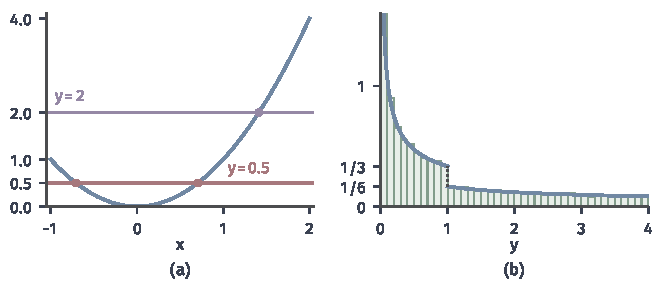
\includegraphics[width=112mm]{figures/07-probability/01-elementary-probability/matplotlib/rvt-square-branches/figure.pdf}
  \caption{多分支的平方变换，$X\sim\operatorname{Unif}(-1,2)$，$Y=X^2$。(a)蓝线是$g$在支撑上的部分，红线$y=0.5$与它有两个交点，紫线$y=2$只有一个。(b)$Y$的密度（蓝）在$y=1$处跳到一半，浅绿直方图是$20000$个模拟样本（种子$11$）。}
  \label{fig:rvt-square-branches}
\end{BookInlineFigure}

\paragraph{绝对值变换}
$Y=\lvert X\rvert$时两支是$x=y$与$x=-y$，导数的绝对值都是$1$，式~\eqref{eq:rvt-branch-density}给出
\[
 f_Y(y)=f_X(y)+f_X(-y),\qquad y>0 .
\]
左半轴的密度被对折到右半轴，与右半轴原有的密度相加。$X\sim\mathcal{N}(0,1)$时得到$f_Y(y)=2\varphi(y)$。

\paragraph{原子质量}
带原子的输入要单独处理原子。离散变量直接用式~\eqref{eq:rvt-discrete-pushforward}：$X$在$\{-2,-1,0,1,2\}$上等可能，则$\lvert X\rvert$的质量为
\[
 p_Y(0)=\frac15,\qquad p_Y(1)=\frac25,\qquad p_Y(2)=\frac25 .
\]

更常见的是混合型的输入。设$X$以概率$0.3$取$0$，以概率$0.7$按$\mathcal{N}(0,1)$取值，即
\[
 F_X(x)=0.3\cdot\mathbf{1}_{\{x\geq0\}}+0.7\,\Phi(x) .
\]
$Y=\lvert X\rvert$在$0$处的原子来自$X$在$0$处的原子，质量$0.3$；其余质量按绝对值公式对折。对$y\geq0$，
\[
 F_Y(y)=\mathbb{P}(-y\leq X\leq y)=0.3+0.7\bigl(2\Phi(y)-1\bigr) .
\]

$Y$在$(0,\infty)$上的连续部分是$0.7\cdot2\varphi(y)$，积分只有$0.7$。若只写出这个“密度”，就丢掉了$0$处的$0.3$；若把它当成完整的密度再归一化，又把原子错误地抹进了连续部分。图~\ref{fig:rvt-abs-atom}画出两个分布函数，原子表现为跳跃，在变换前后保持在$0$处。

\begin{BookInlineFigure}
  \centering
  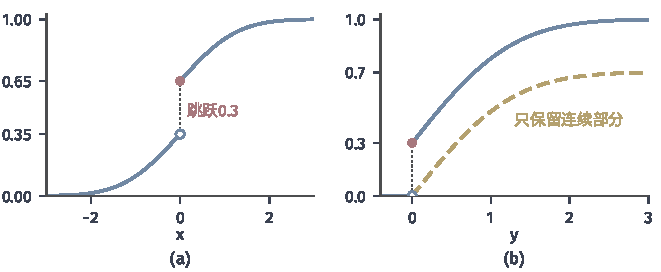
\includegraphics[width=112mm]{figures/07-probability/01-elementary-probability/matplotlib/rvt-abs-atom/figure.pdf}
  \caption{带原子的绝对值变换。(a)$X$的分布函数（蓝），在$0$处跳跃$0.3$（红点）。(b)$Y=\lvert X\rvert$的分布函数（蓝），跳跃保持在$0$；黄色虚线是只保留连续部分$0.7\cdot2\varphi$的累计，它最终只到$0.7$。}
  \label{fig:rvt-abs-atom}
\end{BookInlineFigure}

一元变换的两步做法到此可以总结为：分布函数法总是可用；需要密度时，先把输入切成单调的分支，检查每支上导数不为零，再按式~\eqref{eq:rvt-branch-density}相加；原子与导数为零的区间另算质量。


\section{多元变换}
\label{sec:rvt-multivariate}

随机向量$\bm{X}=(X_1,\ldots,X_d)$有联合密度$f_{\bm{X}}$，$\bm{Y}=\bm{g}(\bm{X})$取值于$\mathbb{R}^{k}$。原像规则~\eqref{eq:rvt-preimage-rule}仍然成立，难处在于原像是$\mathbb{R}^{d}$中的区域，把它的积分换到$\bm{Y}$的坐标上，要先回答三个问题：输入输出的维数是否相同，$\bm{g}$是否一一，是否需要像上一节那样分支。

\paragraph{仿射变换的均值与协方差}
先看最简单的$\bm{Y}=\bm{A}\bm{X}+\bm{b}$，其中$\bm{A}\in\mathbb{R}^{k\times d}$是确定的矩阵，$\bm{b}\in\mathbb{R}^{k}$。设$\bm{X}$有均值向量$\bm{\mu}$与协方差矩阵$\bm{\Sigma}$。由期望的线性性，
\[
 \mathbb{E}[\bm{Y}]=\bm{A}\bm{\mu}+\bm{b} .
\]
中心化之后$\bm{Y}-\mathbb{E}[\bm{Y}]=\bm{A}(\bm{X}-\bm{\mu})$，矩阵$\bm{A}$可以移到期望之外，于是
\begin{equation}
 \operatorname{Cov}(\bm{Y})=\mathbb{E}\bigl[\bm{A}(\bm{X}-\bm{\mu})(\bm{X}-\bm{\mu})^{\top}\bm{A}^{\top}\bigr]=\bm{A}\bm{\Sigma}\bm{A}^{\top} .
 \label{eq:rvt-affine-covariance}
\end{equation}
这两个公式对任何有有限二阶矩的$\bm{X}$都成立，不需要密度。

支撑也跟着变：$\bm{Y}$只在$\bm{X}$的取值范围在仿射映射下的像中取值。$k=d$而$\bm{A}$奇异时，像落在一个低维的仿射子空间里。例如
\[
 \bm{A}=\begin{pmatrix}1&1\\1&1\end{pmatrix},\qquad Y_1=Y_2=X_1+X_2 ,
\]
$\bm{Y}$总在对角线上。对角线在平面上面积为零，$\bm{Y}$没有二维的联合密度；由式~\eqref{eq:rvt-affine-covariance}，$X_1,X_2$独立且方差为$1$时$\operatorname{Cov}(\bm{Y})$的四个元素都是$2$，这个矩阵奇异，与支撑的退化相对应。所以求密度之前要先检查维数与可逆性。

\subsection{可逆变换}
\label{sec:rvt-invertible}

同维且一一的映射是一元单调变换的直接推广。一元时长度伸缩$\lvert g'\rvert$倍；多元时把小区间换成小方块，伸缩的是体积。

\paragraph{体积的伸缩}
可微映射在一点附近近似于线性映射$\bm{x}\mapsto\bm{g}(\bm{x}_0)+D\bm{g}(\bm{x}_0)(\bm{x}-\bm{x}_0)$，其中$D\bm{g}$是Jacobian矩阵。线性映射把任何区域的体积乘以行列式的绝对值，所以边长$\Delta$的小方块被映成体积约为$\lvert\det D\bm{g}(\bm{x}_0)\rvert\Delta^{d}$的小平行体。概率不变而体积放大$\lvert\det D\bm{g}\rvert$倍，密度就要除以这个数。

\begin{theorem}[可逆变换的联合密度]
\label{thm:rvt-multivariate-density}
设$\bm{X}$的联合密度在开集$U\subset\mathbb{R}^{d}$之外为零，$\bm{g}:U\to V=\bm{g}(U)$是一一映射，连续可微，且对所有$\bm{x}\in U$有$\det D\bm{g}(\bm{x})\neq0$。记$\bm{h}=\bm{g}^{-1}$。则$\bm{Y}=\bm{g}(\bm{X})$有联合密度
\begin{equation}
 f_{\bm{Y}}(\bm{y})=
 \begin{cases}
  f_{\bm{X}}\bigl(\bm{h}(\bm{y})\bigr)\,\bigl\lvert\det D\bm{h}(\bm{y})\bigr\rvert, & \bm{y}\in V,\\
  0, & \bm{y}\notin V .
 \end{cases}
 \label{eq:rvt-multivariate-density}
\end{equation}
其中$D\bm{h}$在$\bm{y}$处的行列式等于$D\bm{g}$在$\bm{h}(\bm{y})$处行列式的倒数。
\end{theorem}

\begin{proof}
由反函数定理，$V$是开集，$\bm{h}$连续可微，并且
\[
 D\bm{h}(\bm{y})=\bigl(D\bm{g}(\bm{h}(\bm{y}))\bigr)^{-1} ,
\]
两者的行列式互为倒数。

取闭包含于$V$的矩形$B$。由原像规则，$\bm{Y}\in B$的概率等于$\bm{X}\in\bm{h}(B)$的概率，即$f_{\bm{X}}$在$\bm{h}(B)$上的积分。对它作换元$\bm{x}=\bm{h}(\bm{y})$，得到
\[
 \int_{\bm{h}(B)}f_{\bm{X}}(\bm{x})\,\mathrm{d}\bm{x}=\int_{B}f_{\bm{X}}\bigl(\bm{h}(\bm{y})\bigr)\bigl\lvert\det D\bm{h}(\bm{y})\bigr\rvert\,\mathrm{d}\bm{y} .
\]
矩形上的概率确定了联合分布函数，从而确定联合分布，所以式~\eqref{eq:rvt-multivariate-density}是$\bm{Y}$的密度。$V$无界或$f_{\bm{X}}$在边界附近无界时，先在内部的紧区域上换元，再取极限。
\end{proof}

反函数定理见\BookChapterRef{chap:implicit-inverse-functions}{卷二第22章“隐函数与反函数”}，区域积分的换元公式与极坐标的截断处理见\BookChapterRef{chap:region-integrals}{卷二第24章“区域积分”}。定理的条件与一元时一一对应：一一对应单调，$\det D\bm{g}\neq0$对应$g'\neq0$，$V=\bm{g}(U)$交代输出的支撑。

式~\eqref{eq:rvt-multivariate-density}自带一个检查。对$V$积分，再把换元倒回去，得到
\[
 \int_{V}f_{\bm{Y}}(\bm{y})\,\mathrm{d}\bm{y}=\int_{U}f_{\bm{X}}(\bm{x})\,\mathrm{d}\bm{x}=1 .
\]
算出一个联合密度后，验证它的总积分是$1$，可以发现漏掉的行列式或写错的取值区域。

\paragraph{线性高斯变换}
设$Z_1,\ldots,Z_d$独立且都服从$\mathcal{N}(0,1)$，联合密度是各自密度的乘积：
\[
 f_{\bm{Z}}(\bm{z})=(2\pi)^{-d/2}\exp\Bigl(-\tfrac12\lVert\bm{z}\rVert_2^2\Bigr) .
\]
取可逆矩阵$\bm{A}\in\mathbb{R}^{d\times d}$与向量$\bm{\mu}$，令$\bm{Y}=\bm{A}\bm{Z}+\bm{\mu}$。反函数及其导数是
\[
 \bm{h}(\bm{y})=\bm{A}^{-1}(\bm{y}-\bm{\mu}),\qquad D\bm{h}=\bm{A}^{-1},\qquad \lvert\det D\bm{h}\rvert=\frac{1}{\lvert\det\bm{A}\rvert} .
\]

记$\bm{\Sigma}=\bm{A}\bm{A}^{\top}$，它就是式~\eqref{eq:rvt-affine-covariance}给出的协方差。指数中的平方长度改写为
\[
 \bigl\lVert\bm{A}^{-1}(\bm{y}-\bm{\mu})\bigr\rVert_2^2=(\bm{y}-\bm{\mu})^{\top}\bm{A}^{-\top}\bm{A}^{-1}(\bm{y}-\bm{\mu})=(\bm{y}-\bm{\mu})^{\top}\bm{\Sigma}^{-1}(\bm{y}-\bm{\mu}),
\]
又$\det\bm{\Sigma}=(\det\bm{A})^2$。代入式~\eqref{eq:rvt-multivariate-density}，得到
\begin{equation}
 f_{\bm{Y}}(\bm{y})=\frac{1}{(2\pi)^{d/2}(\det\bm{\Sigma})^{1/2}}\exp\Bigl(-\frac12(\bm{y}-\bm{\mu})^{\top}\bm{\Sigma}^{-1}(\bm{y}-\bm{\mu})\Bigr) .
 \label{eq:rvt-gaussian-density}
\end{equation}

这就是第~\ref{chap:multivariate-distributions}章中$\bm{\Sigma}$正定时$\mathcal{N}(\bm{\mu},\bm{\Sigma})$的密度，现在得到了它的换元依据。结果只通过$\bm{\Sigma}=\bm{A}\bm{A}^{\top}$依赖$\bm{A}$：把$\bm{A}$换成$\bm{A}\bm{Q}$（$\bm{Q}$正交）不改变$\bm{\Sigma}$，因而不改变分布，这对应标准高斯在旋转下不变。$\bm{A}$奇异时$\det\bm{\Sigma}=0$，公式失去意义，这正是前面讲的支撑退化。

下面用一个二维例子核对：
\[
 \bm{A}=\begin{pmatrix}2&0\\1&1\end{pmatrix},\qquad \bm{\mu}=\bm{0} .
\]
$\det\bm{A}=2$，协方差与它的逆分别是
\[
 \bm{\Sigma}=\begin{pmatrix}4&2\\2&2\end{pmatrix},\qquad \bm{\Sigma}^{-1}=\begin{pmatrix}1/2&-1/2\\-1/2&1\end{pmatrix},
\]
$\det\bm{\Sigma}=4$。取$\bm{y}=(2,1)$，它的原像是$\bm{z}=\bm{A}^{-1}\bm{y}=(1,0)$。指数中的两种写法给出同一个数：
\[
 \lVert\bm{z}\rVert_2^2=1,\qquad \bm{y}^{\top}\bm{\Sigma}^{-1}\bm{y}=\tfrac12\cdot4-2\cdot\tfrac12\cdot2+1=1 .
\]
于是
\[
 f_{\bm{Y}}(2,1)=\frac{1}{4\pi}\mathrm{e}^{-1/2}=\frac{f_{\bm{Z}}(1,0)}{\lvert\det\bm{A}\rvert}\approx0.0483 .
\]

图~\ref{fig:rvt-linear-gaussian}画出这个变换。单位正方形被映成面积为$\lvert\det\bm{A}\rvert=2$的平行四边形，两块区域的概率相同，密度降为一半。圆形的等密度线变成椭圆，长轴方向由$\bm{\Sigma}$的特征向量给出。

\begin{BookInlineFigure}
  \centering
  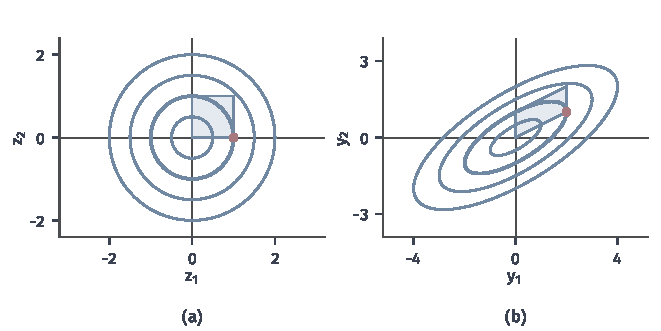
\includegraphics[width=112mm]{figures/07-probability/01-elementary-probability/matplotlib/rvt-linear-gaussian/figure.pdf}
  \caption{线性高斯变换$\bm{Y}=\bm{A}\bm{Z}$，$\bm{A}$的两行为$(2,0)$与$(1,1)$。(a)$\bm{Z}$的等密度线（蓝，圆）与单位正方形（浅蓝），红点为$\bm{z}=(1,0)$。(b)$\bm{Y}$的等密度线（蓝，椭圆）与正方形的像，一个面积为$2$的平行四边形（浅蓝），红点为$\bm{y}=(2,1)$。两幅图的等密度线取同一组$\lVert\bm{z}\rVert_2$值。}
  \label{fig:rvt-linear-gaussian}
\end{BookInlineFigure}

\paragraph{极坐标}
设$X_1,X_2$独立且都服从$\mathcal{N}(0,1)$，问到原点的距离$R$与方向角$\Theta$的分布。映射$(r,\theta)\mapsto(r\cos\theta,r\sin\theta)$把$U=(0,\infty)\times(0,2\pi)$一一地映到平面去掉射线$\{x_1\geq0,\ x_2=0\}$的部分；这条射线面积为零，$(X_1,X_2)$落在上面的概率为零。这里直接把它当作$\bm{h}$，它的Jacobian行列式是
\[
 \det\begin{pmatrix}\cos\theta&-r\sin\theta\\ \sin\theta&r\cos\theta\end{pmatrix}=r .
\]

代入式~\eqref{eq:rvt-multivariate-density}，平方和$x_1^2+x_2^2$变成$r^2$，得到
\begin{equation}
 f_{R,\Theta}(r,\theta)=\frac{1}{2\pi}\mathrm{e}^{-r^2/2}\cdot r=\underbrace{r\,\mathrm{e}^{-r^2/2}}_{R}\cdot\underbrace{\frac{1}{2\pi}}_{\Theta},\qquad r>0,\ 0<\theta<2\pi .
 \label{eq:rvt-polar-density}
\end{equation}
联合密度分解成只含$r$与只含$\theta$的两个因子，所以$R$与$\Theta$独立，$\Theta\sim\operatorname{Unif}(0,2\pi)$，$R$的密度是$r\mathrm{e}^{-r^2/2}$，称为\term{Rayleigh分布}（Rayleigh distribution）。

核对归一化：
\[
 \int_0^\infty r\mathrm{e}^{-r^2/2}\,\mathrm{d}r=\bigl[-\mathrm{e}^{-r^2/2}\bigr]_0^\infty=1 .
\]
由此可算出几个概率：
\[
 \mathbb{P}(R\leq1)=1-\mathrm{e}^{-1/2}\approx0.393,\qquad \mathbb{P}(R>2)=\mathrm{e}^{-2}\approx0.135 .
\]

因子$r$来自面积元。图~\ref{fig:rvt-polar-cell}中，$(r,\theta)$平面上同样大小的小矩形，在$(x_1,x_2)$平面上对应的扇形小块面积约为$r\,\Delta r\,\Delta\theta$，离原点越远越大。所以虽然高斯密度在原点最大，$R$的密度在$r=0$处却是零：靠近原点的圆环面积太小。

\begin{BookInlineFigure}
  \centering
  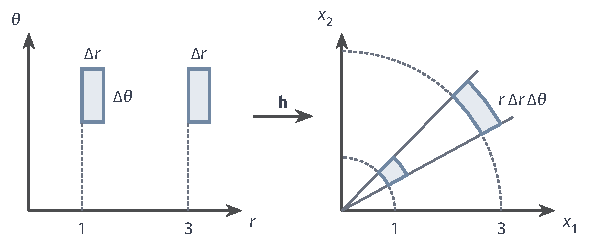
\includegraphics[width=100mm]{figures/07-probability/01-elementary-probability/tikz/rvt-polar-cell/figure.pdf}
  \caption{极坐标的面积元。左侧$(r,\theta)$平面上两个同样大小的矩形（浅蓝），右侧是它们在$(x_1,x_2)$平面上的像，扇形小块的面积约为$r\,\Delta r\,\Delta\theta$，外圈的像比内圈大。}
  \label{fig:rvt-polar-cell}
\end{BookInlineFigure}

再对$W=R^2$用单调变换。$h(w)=\sqrt{w}$，$h'(w)=1/(2\sqrt{w})$，于是
\[
 f_W(w)=\sqrt{w}\,\mathrm{e}^{-w/2}\cdot\frac{1}{2\sqrt{w}}=\frac12\mathrm{e}^{-w/2},\qquad w>0 ,
\]
即$X_1^2+X_2^2\sim\operatorname{Exp}(1/2)$，也就是$\operatorname{Gamma}(1,1/2)=\chi^2_2$。图~\ref{fig:rvt-rayleigh}用模拟样本核对这三个结论。

\begin{BookInlineFigure}
  \centering
  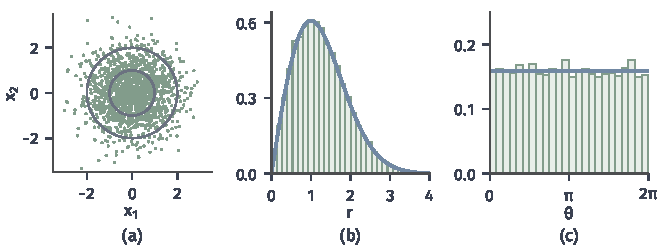
\includegraphics[width=112mm]{figures/07-probability/01-elementary-probability/matplotlib/rvt-rayleigh/figure.pdf}
  \caption{二维标准高斯的极坐标，$20000$个模拟样本（种子$3$）。(a)前$1500$个样本点（绿）与半径$1$、$2$的圆（灰）。(b)$R$的直方图（浅绿）与Rayleigh密度$r\mathrm{e}^{-r^2/2}$（蓝）。(c)$\Theta$的直方图与均匀密度$1/(2\pi)$（蓝）。}
  \label{fig:rvt-rayleigh}
\end{BookInlineFigure}

\paragraph{Gamma归一化}
第~\ref{chap:multivariate-distributions}章用独立Gamma变量除以总和来构造Dirichlet比例，联合密度留到了这里。设$X_1,\ldots,X_d$独立，$X_i\sim\operatorname{Gamma}(\alpha_i,\beta)$，速率$\beta$相同，$d\geq2$。比例$X_i/S$共有$d$个，但它们的和恒为$1$，只有$d-1$个是自由的；只用比例会降维。所以保留总量，取
\[
 S=\sum_{i=1}^{d}X_i,\qquad P_i=\frac{X_i}{S},\quad i=1,\ldots,d-1 ,
\]
这是从$U=(0,\infty)^{d}$到$V=\{(s,\bm{p}):\ s>0,\ p_i>0,\ \sum_{i<d}p_i<1\}$的同维映射。

逆映射是$x_i=sp_i$（$i<d$），$x_d=s(1-p_1-\cdots-p_{d-1})$，所以映射一一。记$p_d=1-\sum_{i<d}p_i$。$\bm{h}$的Jacobian矩阵按列对$s,p_1,\ldots,p_{d-1}$求导，第$i$行（$i<d$）是$(p_i,\ s\bm{e}_i^{\top})$，最后一行是$(p_d,\ -s,\ldots,-s)$。把前$d-1$行都加到最后一行，最后一行变成$(1,0,\ldots,0)$；行列式不变，再按最后一行展开，剩下的子矩阵是$s\bm{I}_{d-1}$，于是
\[
 \bigl\lvert\det D\bm{h}(s,\bm{p})\bigr\rvert=s^{d-1} .
\]

$d=2$时可以直接核对：$x_1=sp$，$x_2=s(1-p)$，行列式是$p\cdot(-s)-s\cdot(1-p)=-s$。

输入的联合密度是各Gamma密度的乘积：
\[
 f_{\bm{X}}(\bm{x})=\prod_{i=1}^{d}\frac{\beta^{\alpha_i}}{\Gamma(\alpha_i)}x_i^{\alpha_i-1}\mathrm{e}^{-\beta x_i}=\frac{\beta^{\alpha_0}\mathrm{e}^{-\beta s}}{\prod_i\Gamma(\alpha_i)}\prod_{i=1}^{d}x_i^{\alpha_i-1},
\]
其中$\alpha_0=\sum_i\alpha_i$，$s=\sum_ix_i$。代入$x_i=sp_i$，乘积变成$s^{\alpha_0-d}\prod_ip_i^{\alpha_i-1}$；再乘以$s^{d-1}$，$s$的幂次是$\alpha_0-1$。按$s$与$\bm{p}$分组，得到
\begin{equation}
 f_{S,\bm{P}}(s,\bm{p})=\underbrace{\frac{\beta^{\alpha_0}}{\Gamma(\alpha_0)}s^{\alpha_0-1}\mathrm{e}^{-\beta s}}_{\operatorname{Gamma}(\alpha_0,\beta)}\cdot\underbrace{\frac{\Gamma(\alpha_0)}{\prod_{i}\Gamma(\alpha_i)}\prod_{i=1}^{d}p_i^{\alpha_i-1}}_{\operatorname{Dir}(\bm{\alpha})} .
 \label{eq:rvt-gamma-dirichlet}
\end{equation}

这一个式子给出四个结论。第一，$S\sim\operatorname{Gamma}(\alpha_0,\beta)$：同速率独立Gamma变量之和仍是Gamma，形状参数相加。第二，比例向量的密度是第二个因子，即$\operatorname{Dir}(\bm{\alpha})$在前$d-1$个自由坐标上的密度。第三，联合密度分解为两个因子，所以总量$S$与比例$\bm{P}$相互独立。第四，$\beta$只出现在第一个因子里，比例的分布与共同速率无关，这就是共同速率被消去的含义。

第二个因子的归一化也随之得到。$f_{S,\bm{P}}$是密度，总积分为$1$；第一个因子对$s$的积分为$1$；所以第二个因子在$V$的$\bm{p}$部分上的积分必为$1$，这就是Dirichlet密度归一化常数的来历。

$d=2$时，比例$P_1=X_1/S$服从$\operatorname{Beta}(\alpha_1,\alpha_2)$。取$\alpha_1=2$、$\alpha_2=3$、$\beta=1$，则$P_1\sim\operatorname{Beta}(2,3)$，均值$2/5$；$S\sim\operatorname{Gamma}(5,1)$，均值$5$。图~\ref{fig:rvt-gamma-simplex}画出两套坐标的对应关系，图~\ref{fig:rvt-dirichlet-check}用模拟核对边缘与独立性。

\begin{BookInlineFigure}
  \centering
  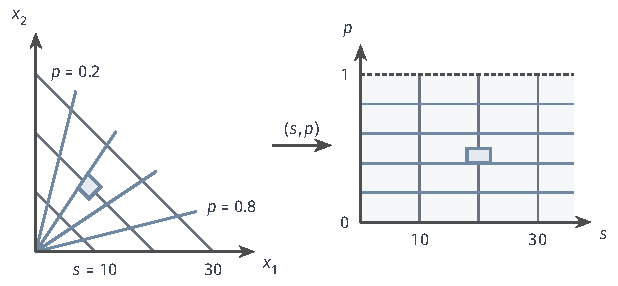
\includegraphics[width=104.7mm]{figures/07-probability/01-elementary-probability/tikz/rvt-gamma-simplex/figure.pdf}
  \caption{总量与比例坐标，$d=2$。左侧第一象限中，灰色斜线是总量$s=x_1+x_2$为常数的线，蓝色射线是比例$p=x_1/s$为常数的线；右侧是对应的$(s,p)$半带。浅蓝小块是$(s,p)$平面上的一个小矩形及其像，像的面积约为$s\,\Delta s\,\Delta p$。}
  \label{fig:rvt-gamma-simplex}
\end{BookInlineFigure}

\begin{BookInlineFigure}
  \centering
  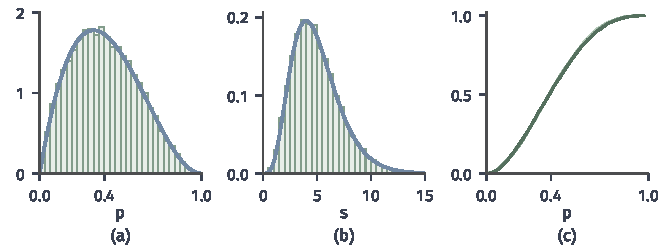
\includegraphics[width=112mm]{figures/07-probability/01-elementary-probability/matplotlib/rvt-dirichlet-check/figure.pdf}
  \caption{Gamma归一化的模拟核对，$X_1\sim\operatorname{Gamma}(2,1)$与$X_2\sim\operatorname{Gamma}(3,1)$独立，$20000$个样本（种子$5$）。(a)$P=X_1/S$的直方图（浅绿）与$\operatorname{Beta}(2,3)$密度（蓝）。(b)$S$的直方图与$\operatorname{Gamma}(5,1)$密度（蓝）。(c)按$S$的三分位数把样本分成三组，三组中$P$的经验分布函数（绿色由浅到深）几乎重合，与$S$独立相符。}
  \label{fig:rvt-dirichlet-check}
\end{BookInlineFigure}

\subsection{多分支与降维}
\label{sec:rvt-branches-reduction}

可逆变换的定理要求同维和一一。两个条件分别失效时，做法与一元时类似：不一一就分支相加，降维就先补足坐标再积掉。

\paragraph{同维多分支}
设$U_1,\ldots,U_m$是互不相交的开集，除去一个面积（体积）为零的集合外覆盖$\bm{X}$的取值范围，$\bm{g}$在每个$U_k$上满足定理~\ref{thm:rvt-multivariate-density}的条件，反函数为$\bm{h}_k$。与定理~\ref{thm:rvt-branch-density}的证明相同，把事件按$\bm{X}$落在哪个$U_k$分解，各分支分别换元再相加，得到
\begin{equation}
 f_{\bm{Y}}(\bm{y})=\sum_{k:\ \bm{y}\in\bm{g}(U_k)}f_{\bm{X}}\bigl(\bm{h}_k(\bm{y})\bigr)\,\bigl\lvert\det D\bm{h}_k(\bm{y})\bigr\rvert .
 \label{eq:rvt-multivariate-branch}
\end{equation}

典型的例子是排序。令$\bm{g}(x_1,x_2)=(\min(x_1,x_2),\max(x_1,x_2))$，输出落在$\{(u,v):\ u<v\}$中。对角线$x_1=x_2$面积为零，去掉之后平面分成$U_1=\{x_1<x_2\}$与$U_2=\{x_1>x_2\}$。在$U_1$上$\bm{g}$是恒等映射，在$U_2$上$\bm{g}$交换两个坐标，两个Jacobian行列式的绝对值都是$1$。于是
\[
 f_{\min,\max}(u,v)=f_{\bm{X}}(u,v)+f_{\bm{X}}(v,u),\qquad u<v .
\]
$X_1,X_2$独立且都服从$\operatorname{Unif}(0,1)$时，结果是三角形$0<u<v<1$上的常数$2$；三角形面积为$1/2$，总积分为$1$。第~\ref{sec:rvt-order-statistics}节把这个计算推广到$n$个变量。

\paragraph{降维映射}
设$Z=X_1+X_2$，映射$\mathbb{R}^2\to\mathbb{R}$。它的导数是$1\times2$的矩阵$(1\ \ 1)$，没有行列式；而且每个$z$的原像是整条直线$\{x_1+x_2=z\}$，不是有限个点，式~\eqref{eq:rvt-multivariate-density}与式~\eqref{eq:rvt-multivariate-branch}都无从套用。

办法是补一个坐标，凑成同维可逆变换。取$W=X_2$，映射$(x_1,x_2)\mapsto(z,w)=(x_1+x_2,x_2)$的逆是$x_1=z-w$、$x_2=w$，Jacobian行列式为$1$。由式~\eqref{eq:rvt-multivariate-density}，
\[
 f_{Z,W}(z,w)=f_{\bm{X}}(z-w,w) .
\]
我们只关心$Z$，把不保留的坐标$w$积掉，就得到边缘密度：
\begin{equation}
 f_Z(z)=\int_{\mathbb{R}}f_{\bm{X}}(z-w,w)\,\mathrm{d}w .
 \label{eq:rvt-sum-completion}
\end{equation}

一般地，若$\bm{Y}=\bm{g}(\bm{X})\in\mathbb{R}^{k}$，$k<d$，且能找到$d-k$个辅助坐标$\bm{W}$使$(\bm{Y},\bm{W})$成为$\bm{X}$的同维可逆变换，就先用式~\eqref{eq:rvt-multivariate-density}求联合密度，再对$\bm{w}$积分。辅助坐标的选法不唯一，只要满足可逆条件，结果都相同；选得好，行列式简单，积分区域也简单。

\paragraph{直接按原像计算}
不便补坐标时，回到分布函数法。仍以$X_1,X_2$独立且都服从$\operatorname{Unif}(0,1)$为例，事件$Z\leq z$的原像是单位正方形中直线$x_1+x_2=z$下方的部分。它的面积分两段计算：
\[
 F_Z(z)=
 \begin{cases}
  z^2/2, & 0\leq z\leq1,\\
  1-(2-z)^2/2, & 1\leq z\leq2 .
 \end{cases}
\]

求导得到三角形密度：$0<z<1$时$f_Z(z)=z$，$1<z<2$时$f_Z(z)=2-z$。用式~\eqref{eq:rvt-sum-completion}也能得到它：被积函数$f_{\bm{X}}(z-w,w)$在$0<w<1$且$0<z-w<1$时为$1$，积分等于这段$w$区间的长度，即$\min(z,2-z)$。

图~\ref{fig:rvt-sum-completion}说明两种做法为什么一致。阈值从$z$增加到$z+\Delta z$时，原像增加了一条斜带，斜带的面积就是$f_Z(z)\Delta z$；式~\eqref{eq:rvt-sum-completion}沿着这条斜带积分，补出的坐标$w$正是斜带上的位置。

\begin{BookInlineFigure}
  \centering
  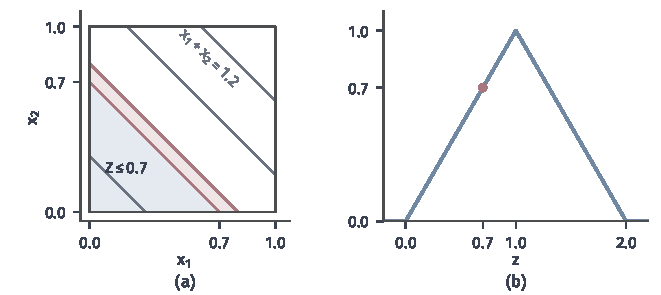
\includegraphics[width=112mm]{figures/07-probability/01-elementary-probability/matplotlib/rvt-sum-completion/figure.pdf}
  \caption{降维映射$Z=X_1+X_2$，$X_1,X_2$独立且服从$\operatorname{Unif}(0,1)$。(a)单位正方形中，浅蓝区域是$Z\leq0.7$的原像，红色斜带是$0.7<Z\leq0.8$的部分，灰线是其他阈值的等值线。(b)$Z$的三角形密度（蓝），红点是$z=0.7$处的值，等于(a)中斜带面积除以$\Delta z=0.1$的极限。}
  \label{fig:rvt-sum-completion}
\end{BookInlineFigure}

其他运算也常这样处理：$\max(X_1,X_2)\leq z$的原像是正方形，$X_1^2+X_2^2\leq z$的原像是圆盘。能写出原像并算出它的概率，就有分布函数；需要密度时再求导。下面四节把这些办法分别用到和、差、乘积、比值和排序上。


\section{和与差}
\label{sec:rvt-sums-differences}

两个随机变量相加或相减，平均与波动怎样变化，前面已经知道。$X,Y$可积时$\mathbb{E}[X\pm Y]=\mathbb{E}[X]\pm\mathbb{E}[Y]$，不需要独立；二阶矩有限时
\[
 \operatorname{Var}(X\pm Y)=\operatorname{Var}(X)+\operatorname{Var}(Y)\pm2\operatorname{Cov}(X,Y) .
\]
但这两个数不能确定$X\pm Y$的分布。第~\ref{sec:rvt-output-distribution}节的三张概率表中，$X+Y$的均值都是$1$，分布却完全不同。这一节求和与差的完整分布。

\subsection{和的分布}
\label{sec:rvt-sum-distribution}

\paragraph{沿斜线累计}
事件$X+Y=z$的原像是平面上的直线$x+y=z$。离散时把直线上各点的联合质量相加；有密度时，式~\eqref{eq:rvt-sum-completion}已经给出沿这条直线的积分。把积分变量记成$x$，两种情形写在一起，就是下面的定理。

\begin{theorem}[和的分布]
\label{thm:rvt-sum-distribution}
设$Z=X+Y$。若$(X,Y)$离散，联合质量为$p_{X,Y}$，则
\begin{equation}
 p_Z(z)=\sum_{x}p_{X,Y}(x,z-x) .
 \label{eq:rvt-discrete-sum}
\end{equation}
若$(X,Y)$有联合密度$f_{X,Y}$，则
\begin{equation}
 f_Z(z)=\int_{\mathbb{R}}f_{X,Y}(x,z-x)\,\mathrm{d}x .
 \label{eq:rvt-density-sum}
\end{equation}
若$X$与$Y$还相互独立，联合规律分解为边缘之积，上两式分别成为
\begin{equation}
 p_Z(z)=\sum_{x}p_X(x)\,p_Y(z-x),\qquad f_Z(z)=\int_{\mathbb{R}}f_X(x)\,f_Y(z-x)\,\mathrm{d}x .
 \label{eq:rvt-convolution}
\end{equation}
\end{theorem}

\begin{proof}
离散情形，事件$Z=z$按$X$的取值分解为互不相交的事件$\{X=x,\ Y=z-x\}$，相加即得式~\eqref{eq:rvt-discrete-sum}。密度情形，在式~\eqref{eq:rvt-sum-completion}中把$(X_1,X_2)$换成$(X,Y)$，并把补出的坐标取为$X$本身（逆映射$x=w$、$y=z-w$，Jacobian行列式的绝对值仍为$1$），再把积分变量$w$改记为$x$，即得式~\eqref{eq:rvt-density-sum}。独立时代入$p_{X,Y}=p_Xp_Y$或$f_{X,Y}=f_Xf_Y$。
\end{proof}

式~\eqref{eq:rvt-convolution}右端的两种运算分别称为\term{离散卷积}（discrete convolution）与\term{卷积}（convolution），记作$p_X*p_Y$与$f_X*f_Y$。式~\eqref{eq:rvt-density-sum}不需要独立，但需要联合密度；式~\eqref{eq:rvt-convolution}只用边缘，代价是独立的假设。第~\ref{sec:rvt-output-distribution}节的例子说明，没有独立时用边缘作卷积会得到错误的答案。

\paragraph{卷积的读法}
固定$z$，把$f_Y$左右翻转再右移$z$，得到函数$x\mapsto f_Y(z-x)$；它与$f_X$逐点相乘再积分，就是$f_Z(z)$。在两个均匀变量的例子里，两个函数都是高度为$1$的方块，乘积是两个方块重叠部分上的$1$，积分等于重叠的长度。$z$从$0$增加到$1$，重叠从$0$增加到$1$；$z$从$1$增加到$2$，重叠又减到$0$。这正是上一节算出的三角形密度。

图~\ref{fig:rvt-convolution-slide}画出$z=0.7$与$z=1.4$两个位置。按质量的语言，$f_Z(z)$收集了所有满足$x+y=z$的输入对的质量，每一对的权重是$f_X(x)f_Y(z-x)$；滑动的方块只是把“哪些$x$与$z-x$同时可能”画了出来。

\begin{BookInlineFigure}
  \centering
  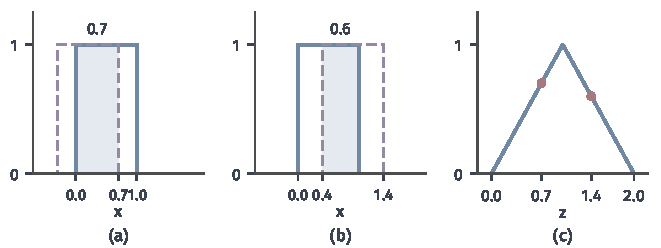
\includegraphics[width=112mm]{figures/07-probability/01-elementary-probability/matplotlib/rvt-convolution-slide/figure.pdf}
  \caption{卷积作为滑动重叠，$f_X=f_Y=\mathbf{1}_{(0,1)}$。(a)$z=0.7$：蓝色方块为$f_X$，紫色方块为翻转平移后的$f_Y(z-x)$，浅蓝重叠长度为$0.7$。(b)$z=1.4$，重叠长度为$0.6$。(c)$f_Z=f_X*f_Y$（蓝），红点是$z=0.7$与$z=1.4$处的值。}
  \label{fig:rvt-convolution-slide}
\end{BookInlineFigure}

\paragraph{骰子的卷积}
两枚骰子各自的质量是$\{1,\ldots,6\}$上的$1/6$。由式~\eqref{eq:rvt-convolution}，$p_Z(z)$等于$1/36$乘以满足$1\leq x\leq6$且$1\leq z-x\leq6$的整数$x$的个数。这些$x$从$\max(1,z-6)$到$\min(6,z-1)$，个数是$6-\lvert z-7\rvert$，与第~\ref{sec:rvt-output-distribution}节数格子的结果相同。

再与第三枚骰子作卷积，就得到三枚骰子之和的质量，取值从$3$到$18$。例如和为$10$时，把两枚之和的质量与第三枚的$1/6$相乘求和，得到
\[
 p_3(10)=\frac16\sum_{x=4}^{9}p_2(x)=\frac16\cdot\frac{3+4+5+6+5+4}{36}=\frac{27}{216}=\frac18 .
\]
卷积满足交换律与结合律，这对应于加法的次序不影响和；所以三枚骰子可以按任意次序逐个加入。图~\ref{fig:rvt-dice-convolution}显示，每多一次卷积，质量就向中间聚得更圆。

\begin{BookInlineFigure}
  \centering
  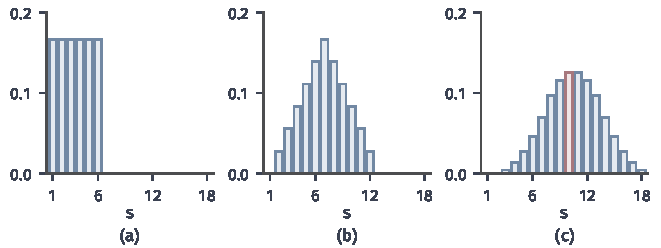
\includegraphics[width=112mm]{figures/07-probability/01-elementary-probability/matplotlib/rvt-dice-convolution/figure.pdf}
  \caption{骰子点数和的质量，由逐次离散卷积算出。(a)一枚；(b)两枚，三角形；(c)三枚，红色柱是和为$10$的质量$1/8$。}
  \label{fig:rvt-dice-convolution}
\end{BookInlineFigure}

连续的情形也一样。$n$个独立的$\operatorname{Unif}(0,1)$之和，$n=2$时是三角形，$n=3$时由三段二次多项式拼成，$n=4$时由四段三次多项式拼成，每加一次，曲线就光滑一阶。图~\ref{fig:rvt-uniform-sums}中，$n=4$时的密度已经和均值$2$、方差$4/12$的高斯密度非常接近。这种逼近在什么意义下、以什么速度成立，以及样本平均怎样集中到均值附近，是第~\ref{chap:laws-of-large-numbers}章与第~\ref{chap:central-limit-theorem}章的内容；这里只需要知道，每一步都是一次卷积。

\begin{BookInlineFigure}
  \centering
  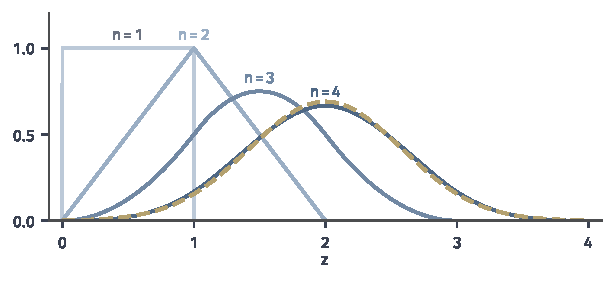
\includegraphics[width=104mm]{figures/07-probability/01-elementary-probability/matplotlib/rvt-uniform-sums/figure.pdf}
  \caption{$n$个独立$\operatorname{Unif}(0,1)$之和的密度，$n=1,2,3,4$（蓝色由浅到深），由逐次数值卷积算出。黄色虚线是均值$2$、方差$1/3$的高斯密度，与$n=4$的曲线对照。}
  \label{fig:rvt-uniform-sums}
\end{BookInlineFigure}

\paragraph{封闭的分布族}
有些分布族在独立相加下封闭：和仍在同一族中，参数按简单的规则相加。这能省去卷积计算，但每一条都有条件。

二项分布。设$X\sim\operatorname{Bin}(m,p)$与$Y\sim\operatorname{Bin}(n,p)$独立，成功概率相同，记$q=1-p$。由式~\eqref{eq:rvt-convolution}，$p$与$q$的幂次在每一项中都是$p^kq^{m+n-k}$，可以提出来：
\[
 p_Z(k)=\sum_{j}\binom{m}{j}p^{j}q^{m-j}\binom{n}{k-j}p^{k-j}q^{n-k+j}=p^{k}q^{m+n-k}\sum_{j}\binom{m}{j}\binom{n}{k-j} .
\]
最后的和数的是从$m+n$个对象中选$k$个、其中$j$个来自前$m$个的方法数，对$j$求和就是$\binom{m+n}{k}$。于是$X+Y\sim\operatorname{Bin}(m+n,p)$：$m$次试验接着$n$次试验，共$m+n$次。

成功概率不同时这条结论不成立。$\operatorname{Bin}(1,1/2)$与$\operatorname{Bin}(1,1/3)$独立相加，和的质量是
\[
 p_Z(0)=\frac13,\qquad p_Z(1)=\frac12,\qquad p_Z(2)=\frac16 .
\]
若它是$\operatorname{Bin}(2,r)$，由均值$2r=5/6$得$r=5/12$，于是应有$p_Z(0)=(7/12)^2=49/144$，与$1/3=48/144$不符。

Poisson分布。设$X\sim\operatorname{Poisson}(\lambda)$与$Y\sim\operatorname{Poisson}(\mu)$独立。卷积中提出$\mathrm{e}^{-(\lambda+\mu)}/k!$，剩下的和由二项式定理求出：
\[
 \begin{aligned}
 p_Z(k)&=\sum_{j=0}^{k}\frac{\mathrm{e}^{-\lambda}\lambda^{j}}{j!}\cdot\frac{\mathrm{e}^{-\mu}\mu^{k-j}}{(k-j)!}
 =\frac{\mathrm{e}^{-(\lambda+\mu)}}{k!}\sum_{j=0}^{k}\binom{k}{j}\lambda^{j}\mu^{k-j}\\
 &=\frac{\mathrm{e}^{-(\lambda+\mu)}(\lambda+\mu)^{k}}{k!} .
 \end{aligned}
\]
即$X+Y\sim\operatorname{Poisson}(\lambda+\mu)$，强度相加，参数不必相同。

高斯分布。设$X\sim\mathcal{N}(\mu_1,\sigma_1^2)$与$Y\sim\mathcal{N}(\mu_2,\sigma_2^2)$独立，$\sigma_1,\sigma_2>0$。由线性变换的结论，可以写成
\[
 X=\mu_1+\sigma_1Z_1,\qquad Y=\mu_2+\sigma_2Z_2 ,
\]
其中$Z_1,Z_2$独立且都是标准高斯。令$s=\sqrt{\sigma_1^2+\sigma_2^2}$。取第一行为$(\sigma_1,\sigma_2)/s$的$2\times2$正交矩阵$\bm{Q}$，由上一节的结论，$\bm{Q}\bm{Z}$的协方差是$\bm{Q}\bm{Q}^{\top}=\bm{I}$，与$\bm{Z}$同分布，所以它的第一个分量$(\sigma_1Z_1+\sigma_2Z_2)/s$服从$\mathcal{N}(0,1)$。于是
\begin{equation}
 X+Y=\mu_1+\mu_2+s\cdot\frac{\sigma_1Z_1+\sigma_2Z_2}{s}\sim\mathcal{N}\bigl(\mu_1+\mu_2,\ \sigma_1^2+\sigma_2^2\bigr) .
 \label{eq:rvt-gaussian-sum}
\end{equation}
直接计算卷积并对指数配方，也得到同样的结果。

Gamma分布与$\chi^2$分布。式~\eqref{eq:rvt-gamma-dirichlet}的第一个因子已经说明，同速率的独立Gamma变量之和服从$\operatorname{Gamma}(\alpha_0,\beta)$。因为$\chi^2_\nu=\operatorname{Gamma}(\nu/2,1/2)$，独立的$\chi^2$变量相加时自由度相加。再结合式~\eqref{eq:rvt-chi2-one}，$Z_1,\ldots,Z_\nu$独立标准高斯时
\begin{equation}
 Z_1^2+\cdots+Z_\nu^2\sim\chi^2_\nu,\qquad \nu=1,2,\ldots
 \label{eq:rvt-chi2-sum}
\end{equation}
$\nu=2$时与极坐标一段算出的$\operatorname{Exp}(1/2)$一致。

\paragraph{独立不能省}
封闭性中的独立不能换成“边缘属于同一族”。取$X\sim\mathcal{N}(0,1)$，再取与$X$独立、以各$1/2$的概率取$\pm1$的随机符号$S$，令$Y=SX$。由于$X$与$-X$同分布，
\[
 \mathbb{P}(Y\leq y)=\tfrac12\mathbb{P}(X\leq y)+\tfrac12\mathbb{P}(-X\leq y)=\Phi(y),
\]
$Y$也服从$\mathcal{N}(0,1)$。由$S$与$X$独立，
\[
 \operatorname{Cov}(X,Y)=\mathbb{E}[SX^2]=\mathbb{E}[S]\,\mathbb{E}[X^2]=0 ,
\]
两者不相关。

可是$X+Y=(1+S)X$：$S=-1$时它等于$0$，$S=1$时它等于$2X$。于是$\mathbb{P}(X+Y=0)=1/2$，和在$0$处有原子，不是高斯分布，更不是式~\eqref{eq:rvt-gaussian-sum}预言的$\mathcal{N}(0,2)$。图~\ref{fig:rvt-closure-counter}画出两者的分布函数。这里$X$与$Y$不相关但不独立，$(X,Y)$也不是联合高斯；只有联合高斯时不相关才推出独立，那是第~\ref{chap:multivariate-distributions}章的结论。

\begin{BookInlineFigure}
  \centering
  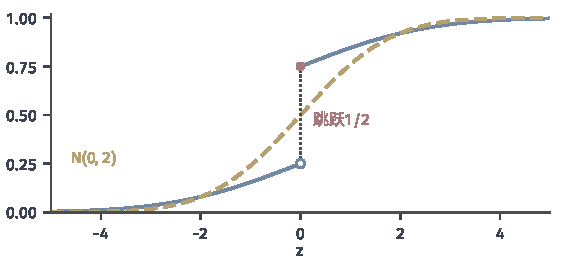
\includegraphics[width=96mm]{figures/07-probability/01-elementary-probability/matplotlib/rvt-closure-counter/figure.pdf}
  \caption{两个不相关的标准高斯之和。蓝线是$X+SX$的分布函数，它在$0$处跳跃$1/2$（红点），其余部分是$\tfrac12\Phi(z/2)$；黄色虚线是独立时的$\mathcal{N}(0,2)$分布函数。}
  \label{fig:rvt-closure-counter}
\end{BookInlineFigure}

\subsection{差的分布}
\label{sec:rvt-difference-distribution}

差可以看成和：$X-Y=X+(-Y)$。由线性变换的密度公式~\eqref{eq:rvt-linear-density}取$a=-1$，$-Y$的密度是$f_Y(-y)$，也就是把$f_Y$左右反射；离散时$-Y$的质量是$p_Y(-y)$。

\paragraph{反射后卷积}
把$-Y$代入定理~\ref{thm:rvt-sum-distribution}。一般情形下$X-Y=z$的原像是直线$y=x-z$，于是$f_{X-Y}(z)=\int f_{X,Y}(x,x-z)\,\mathrm{d}x$；$X$与$Y$独立时，$X$与$-Y$也独立（定理~\ref{thm:rvt-group-independence}），于是
\begin{equation}
 f_{X-Y}(z)=\int_{\mathbb{R}}f_X(x)\,f_Y(x-z)\,\mathrm{d}x .
 \label{eq:rvt-difference-density}
\end{equation}
离散时把积分换成求和。

两枚骰子之差$D=X_1-X_2$取$-5$到$5$的整数。与和的计算相同地数格子，或用离散版的式~\eqref{eq:rvt-difference-density}，得到
\[
 \mathbb{P}(D=d)=\frac{6-\lvert d\rvert}{36},\qquad d=-5,\ldots,5 .
\]
它与和的质量形状相同，只是中心从$7$移到$0$。两个独立$\operatorname{Unif}(0,1)$之差的密度同样是三角形，即$(-1,1)$上的$1-\lvert z\rvert$。

\paragraph{依赖改变差}
差对依赖关系很敏感。设$U,V$都服从$\operatorname{Unif}(0,1)$，比较三种联合规律：
\begin{itemize}
 \item $U,V$独立：$U-V$的密度是$1-\lvert z\rvert$，方差$1/6$；
 \item $V=U$：$U-V$恒为$0$，全部质量是一个原子，方差$0$；
 \item $V=1-U$：$U-V=2U-1\sim\operatorname{Unif}(-1,1)$，方差$1/3$。
\end{itemize}
三种情形的方差都符合
\[
 \operatorname{Var}(U-V)=\tfrac1{12}+\tfrac1{12}-2\operatorname{Cov}(U,V),
\]
协方差分别是$0$、$1/12$、$-1/12$。

协方差项前的负号有直接的解释。正相关时两个变量倾向于同时偏大或同时偏小，偏差在相减时相互抵消，差的波动变小；负相关时一个偏大另一个就偏小，相减反而叠加。和的情形正好相反，所以$\operatorname{Var}(X+Y)$中协方差项带正号。

联合高斯的情形可以写出完整的分布。设$(X,Y)$联合高斯，两个边缘都是$\mathcal{N}(0,1)$，相关系数为$\rho$。联合高斯向量的线性组合仍是高斯（第~\ref{chap:multivariate-distributions}章），由方差公式得到
\[
 X-Y\sim\mathcal{N}(0,\,2-2\rho),\qquad X+Y\sim\mathcal{N}(0,\,2+2\rho) .
\]
$\rho=0.8$时差的方差是$0.4$，$\rho=-0.8$时是$3.6$。图~\ref{fig:rvt-difference-dependence}把两组例子放在一起：边缘完全相同，只是联合规律不同，差的分布就从一个点变成三角形，再变成一段平坦的区间。

\begin{BookInlineFigure}
  \centering
  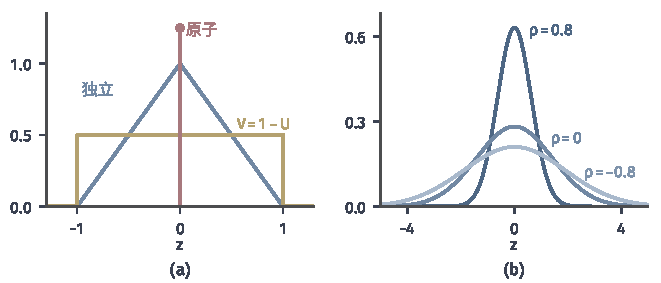
\includegraphics[width=112mm]{figures/07-probability/01-elementary-probability/matplotlib/rvt-difference-dependence/figure.pdf}
  \caption{相同边缘、不同依赖下的差。(a)$U,V\sim\operatorname{Unif}(0,1)$：独立时$U-V$的密度（蓝，三角形），$V=1-U$时的密度（黄，平坦），$V=U$时$0$处的原子（红色竖线，质量$1$）。(b)联合高斯、标准边缘、相关系数$\rho=0.8,0,-0.8$时$X-Y$的密度（蓝色由深到浅），方差分别为$0.4$、$2$、$3.6$。}
  \label{fig:rvt-difference-dependence}
\end{BookInlineFigure}

所以，和与差的分布由联合规律决定；均值与方差由边缘和协方差决定；只有在独立时，完整分布才能由边缘的卷积算出。


\section{乘积的分布}
\label{sec:rvt-products}

一块矩形木板的长和宽都是随机的，面积$Z=XY$服从什么分布？取最简单的情形：$X,Y$独立且都服从$\operatorname{Unif}(0,1)$。面积也在$(0,1)$中，但它会更偏向小值，因为两个小于$1$的数相乘只会更小。偏多少，要算出来。

\paragraph{直接按原像计算}
事件$XY\leq z$（$0<z<1$）的原像是单位正方形中双曲线$xy=z$下方的部分。$x\leq z$时整段竖线都在原像中；$x>z$时竖线上满足$y\leq z/x$的部分在原像中。于是
\[
 F_Z(z)=z+\int_z^1\frac{z}{x}\,\mathrm{d}x=z-z\ln z .
\]
求导，$1-\ln z-1=-\ln z$，得到
\begin{equation}
 f_Z(z)=-\ln z,\qquad 0<z<1 .
 \label{eq:rvt-uniform-product}
\end{equation}
它在$z\to0$时趋于无穷，但可积。

\paragraph{辅助坐标}
一般情形用上一节的降维办法：补一个坐标，凑成同维可逆变换。取$W=X$，映射$(x,y)\mapsto(w,z)=(x,xy)$在$x\neq0$的区域上一一，逆映射是$x=w$、$y=z/w$。它的Jacobian行列式是
\[
 \det\begin{pmatrix}1&0\\-z/w^{2}&1/w\end{pmatrix}=\frac1w .
\]

要使用这个变换，需要$\mathbb{P}(X=0)=0$，这样去掉直线$x=0$不损失质量。$(X,Y)$有联合密度时这自动成立，因为直线面积为零。由式~\eqref{eq:rvt-multivariate-density}得到$f_{W,Z}(w,z)=f_{X,Y}(w,z/w)/\lvert w\rvert$，再积掉$w$并改记为$x$，就得到下面的公式。

\begin{theorem}[乘积的密度]
\label{thm:rvt-product-density}
设$(X,Y)$有联合密度$f_{X,Y}$，则$Z=XY$有密度
\begin{equation}
 f_Z(z)=\int_{\mathbb{R}}f_{X,Y}\Bigl(x,\frac zx\Bigr)\frac{1}{\lvert x\rvert}\,\mathrm{d}x .
 \label{eq:rvt-product-density}
\end{equation}
若$X$与$Y$独立，被积函数中的$f_{X,Y}(x,z/x)$换成$f_X(x)\,f_Y(z/x)$。
\end{theorem}

因子$1/\lvert x\rvert$可以这样理解。固定$X=x$，$Z$落在$[z,z+\Delta z]$等价于$Y$落在长度为$\Delta z/\lvert x\rvert$的区间里。$x$越接近零，$Z$的同一段小区间要求$Y$变动的范围越大，收集到的质量越多。乘积的密度在零附近常常变大，原因就在这里。

\paragraph{均匀变量的核对}
把$f_X=f_Y=\mathbf{1}_{(0,1)}$代入式~\eqref{eq:rvt-product-density}。被积函数非零要求$0<x<1$且$0<z/x<1$，即$z<x<1$，于是
\[
 f_Z(z)=\int_z^1\frac{\mathrm{d}x}{x}=-\ln z ,
\]
与直接计算的式~\eqref{eq:rvt-uniform-product}一致。支撑是$(0,1)$，归一化为
\[
 \int_0^1(-\ln z)\,\mathrm{d}z=\bigl[z-z\ln z\bigr]_0^1=1 ,
\]
其中用到了$z\ln z\to0$（$z\to0$）。

数值特征也能核对。独立时$\mathbb{E}[XY]=\mathbb{E}[X]\,\mathbb{E}[Y]=1/4$，而由密度计算
\[
 \int_0^1z(-\ln z)\,\mathrm{d}z=\frac14 .
\]
中位数$m$满足$m-m\ln m=1/2$，数值求解得$m\approx0.187$，远小于均值$0.25$：大部分面积都很小，少数接近$1$的面积把均值拉高。

还有一条独立的路径：对正变量，乘积取对数变成和。由第~\ref{sec:rvt-monotone}节，$-\ln X$与$-\ln Y$都服从$\operatorname{Exp}(1)=\operatorname{Gamma}(1,1)$，由定理~\ref{thm:rvt-group-independence}它们独立；按上一节的Gamma封闭性，它们的和$G=-\ln Z$服从$\operatorname{Gamma}(2,1)$，密度$g\mathrm{e}^{-g}$。再对递减变换$Z=\mathrm{e}^{-G}$用式~\eqref{eq:rvt-monotone-density}，$\lvert h'(z)\rvert=1/z$，得到
\[
 f_Z(z)=(-\ln z)\,\mathrm{e}^{\ln z}\cdot\frac1z=-\ln z .
\]
三种算法给出同一个结果。

图~\ref{fig:rvt-product-uniform}(a)画出原像，(b)用模拟样本核对密度。

\paragraph{符号}
输入可正可负时，式~\eqref{eq:rvt-product-density}自动处理符号，只需注意$z/x$的符号随$x$改变。设$X,Y$独立且都服从$\operatorname{Unif}(-1,1)$，密度各为$1/2$。被积函数非零要求$\lvert x\rvert<1$且$\lvert z/x\rvert<1$，即$\lvert z\rvert<\lvert x\rvert<1$，正负两段$x$对称，于是
\[
 f_Z(z)=\frac14\cdot2\int_{\lvert z\rvert}^{1}\frac{\mathrm{d}x}{x}=-\frac12\ln\lvert z\rvert,\qquad 0<\lvert z\rvert<1 .
\]
它是$-\ln z$对折成的偶函数，总积分仍为$1$。

\paragraph{零处的原子}
输入在零处有原子时，辅助坐标的条件$\mathbb{P}(X=0)=0$失效，要把零单独算。乘积为零当且仅当至少一个因子为零：
\[
 \mathbb{P}(XY=0)=\mathbb{P}(X=0)+\mathbb{P}(Y=0)-\mathbb{P}(X=0,\ Y=0) .
\]
其余的质量在$X\neq0$、$Y\neq0$的部分上按式~\eqref{eq:rvt-product-density}计算。

例如一台机器以概率$0.3$停工、产量为零，以概率$0.7$开工、产量占满负荷的比例服从$\operatorname{Unif}(0,1)$，再乘以一个独立的$\operatorname{Unif}(0,1)$的合格率。设$B\sim\operatorname{Bern}(0.7)$、$X'$、$Y$相互独立，$X',Y\sim\operatorname{Unif}(0,1)$，产量$X=BX'$，合格产量$Z=XY$。则$\mathbb{P}(Z=0)=\mathbb{P}(B=0)=0.3$；$B=1$时$Z=X'Y$，所以$Z$在$(0,1)$上的连续部分是$0.7\cdot(-\ln z)$。分布函数是
\[
 F_Z(z)=0.3+0.7\,(z-z\ln z),\qquad 0\leq z<1 .
\]
若对$X$的“密度部分”$0.7\cdot\mathbf{1}_{(0,1)}$直接套用式~\eqref{eq:rvt-product-density}而不另计原子，总质量只有$0.7$。

\begin{BookInlineFigure}
  \centering
  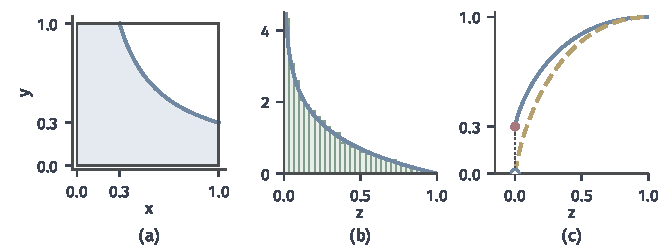
\includegraphics[width=112mm]{figures/07-probability/01-elementary-probability/matplotlib/rvt-product-uniform/figure.pdf}
  \caption{两个独立$\operatorname{Unif}(0,1)$的乘积。(a)浅蓝区域是$XY\leq0.3$的原像，蓝线为双曲线$xy=0.3$，面积$0.3-0.3\ln0.3\approx0.661$。(b)密度$-\ln z$（蓝）与$20000$个模拟样本的直方图（浅绿，种子$13$）。(c)$X$在零处有$0.3$的原子时乘积的分布函数（蓝），红点表示零处的原子，黄色虚线是没有原子时的$z-z\ln z$。}
  \label{fig:rvt-product-uniform}
\end{BookInlineFigure}

乘积的公式与和的公式结构相同，都是“补一个坐标、积掉它”；不同的是乘积的变换在$x=0$处不可逆，所以多了$1/\lvert x\rvert$这个因子，也多了对零处原子的检查。


\section{比值的分布}
\label{sec:rvt-ratios}

两段独立的等待时间之比、一个测量误差除以另一个估计出来的尺度，都是比值$R=X/Y$。比值与乘积只差一个倒数，但分母可以很接近零，这时比值会非常大。这一节的主题是这种情况怎样影响比值的尾部与矩。

\paragraph{分母不能取零}
$R=X/Y$要有定义，首先需要$\mathbb{P}(Y=0)=0$。$(X,Y)$有联合密度时这自动成立；离散时要事先排除$Y$取零的情形，或者把它作为“比值无定义”的事件单独报告。

离散时仍用原像规则：$R=r$当且仅当$(X,Y)$落在直线$x=ry$上的格点之一。两枚骰子的比值$X_1/X_2=2$的原像是$\{(2,1),(4,2),(6,3)\}$，于是
\[
 \mathbb{P}\Bigl(\frac{X_1}{X_2}=2\Bigr)=\frac{3}{36}=\frac1{12},\qquad \mathbb{P}\Bigl(\frac{X_1}{X_2}=1\Bigr)=\frac{6}{36}=\frac16 .
\]

\paragraph{比值与分母的联合换元}
有密度时，取辅助坐标$W=Y$。映射$(x,y)\mapsto(r,w)=(x/y,y)$在$y\neq0$的区域上一一，逆映射是$x=rw$、$y=w$，Jacobian行列式为
\[
 \det\begin{pmatrix}w&r\\0&1\end{pmatrix}=w .
\]
由式~\eqref{eq:rvt-multivariate-density}得到$f_{R,W}(r,w)=f_{X,Y}(rw,w)\lvert w\rvert$，再积掉$w$，就得到下面的公式。

\begin{theorem}[比值的密度]
\label{thm:rvt-ratio-density}
设$(X,Y)$有联合密度$f_{X,Y}$，则$R=X/Y$有密度
\begin{equation}
 f_R(r)=\int_{\mathbb{R}}f_{X,Y}(rw,w)\,\lvert w\rvert\,\mathrm{d}w .
 \label{eq:rvt-ratio-density}
\end{equation}
若$X$与$Y$独立，被积函数中的$f_{X,Y}(rw,w)$换成$f_X(rw)\,f_Y(w)$。
\end{theorem}

与乘积公式中的$1/\lvert x\rvert$相反，这里的因子是$\lvert w\rvert$。固定分母$Y=w$，$R$落在$[r,r+\Delta r]$等价于$X$落在长度为$\lvert w\rvert\Delta r$的区间里；分母越小，同样一段$\Delta r$对应的$X$区间越短。所以分母接近零的样本并不集中在某个$r$附近，而是散到很大的$\lvert r\rvert$上去。

\paragraph{均匀变量之比}
设$U,V$独立且都服从$\operatorname{Unif}(0,1)$，$R=U/V$取值于$(0,\infty)$。代入式~\eqref{eq:rvt-ratio-density}，被积函数非零要求$0<w<1$且$0<rw<1$，即$0<w<\min(1,1/r)$，于是
\[
 f_R(r)=\int_0^{\min(1,1/r)}w\,\mathrm{d}w=
 \begin{cases}
  1/2, & 0<r\leq1,\\
  1/(2r^2), & r>1 .
 \end{cases}
\]

在单位正方形里直接看原像也能得到它。$U/V\leq r$即$u\leq rv$，是直线$u=rv$下方的部分：$r\leq1$时是面积为$r/2$的三角形，$r>1$时是正方形去掉面积为$1/(2r)$的三角形。于是
\[
 F_R(r)=
 \begin{cases}
  r/2, & 0<r\leq1,\\
  1-1/(2r), & r>1 .
 \end{cases}
\]
$F_R(1)=1/2$，与$U,V$对称一致。

尾概率$\mathbb{P}(R>r)=1/(2r)$衰减得很慢，均值不存在：
\[
 \mathbb{E}[R]\geq\int_1^\infty r\cdot\frac{1}{2r^2}\,\mathrm{d}r=\infty .
\]
用独立性也能看出这一点：$\mathbb{E}[U/V]=\mathbb{E}[U]\,\mathbb{E}[1/V]$，而$\mathbb{E}[1/V]=\int_0^1v^{-1}\,\mathrm{d}v$发散。分子与分母都有界，比值的均值却是无穷，原因全在分母靠近零的那一小块：$V<\varepsilon$的概率是$\varepsilon$，而在这个事件上$R>U/\varepsilon$。

\paragraph{独立标准高斯之比}
设$X,Y$独立且都服从$\mathcal{N}(0,1)$。由式~\eqref{eq:rvt-ratio-density}，两个高斯密度的乘积给出指数$-(r^2w^2+w^2)/2$；被积函数关于$w$是偶函数，只算$w>0$再乘$2$，得到
\begin{equation}
 f_R(r)=\frac{2}{2\pi}\int_0^\infty w\,\mathrm{e}^{-(1+r^2)w^2/2}\,\mathrm{d}w=\frac{1}{\pi(1+r^2)},\qquad r\in\mathbb{R} .
 \label{eq:rvt-cauchy}
\end{equation}
这是第~\ref{chap:common-distributions}章的Cauchy分布，即自由度为$1$的t分布。

几何上看得更清楚。由式~\eqref{eq:rvt-polar-density}，$(X,Y)$的方向角$\Theta$服从均匀分布，且与半径独立；比值$Y/X=\tan\Theta$只取决于方向，与半径无关。$\tan$以$\pi$为周期，所以$\Theta$只需看作$(-\pi/2,\pi/2)$上的均匀变量，于是
\[
 \mathbb{P}\Bigl(\frac YX\leq t\Bigr)=\frac{\arctan t+\pi/2}{\pi} ,
\]
求导就是式~\eqref{eq:rvt-cauchy}。由对称性$X/Y$与$Y/X$同分布。这个论证只用了方向均匀，所以任何联合密度只依赖于$x^2+y^2$的$(X,Y)$，比值都是Cauchy分布。

图~\ref{fig:rvt-ratio-uniform}(c)中，$Y/X\leq1$的原像是两个对顶的扇形，张角合计$3\pi/2$，占整个圆周的$3/4$，所以$\mathbb{P}(Y/X\leq1)=3/4$，与上式在$t=1$处的值一致。

\begin{BookInlineFigure}
  \centering
  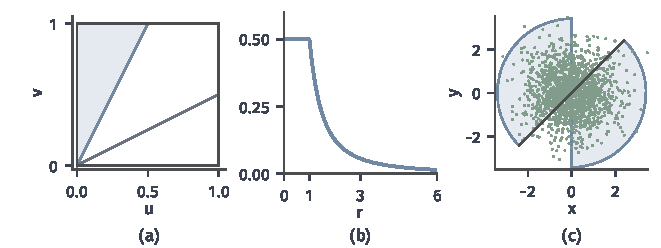
\includegraphics[width=112mm]{figures/07-probability/01-elementary-probability/matplotlib/rvt-ratio-uniform/figure.pdf}
  \caption{比值的原像。(a)$U,V\sim\operatorname{Unif}(0,1)$独立，浅蓝区域是$U/V\leq0.5$的原像，面积$1/4$；灰线是$U/V=2$。(b)$U/V$的密度（蓝），$r>1$后按$1/(2r^2)$衰减。(c)独立标准高斯，浅蓝的两个对顶扇形是$Y/X\leq1$的原像，绿点是$1500$个模拟样本（种子$17$）。}
  \label{fig:rvt-ratio-uniform}
\end{BookInlineFigure}

Cauchy分布的尾部是
\[
 \mathbb{P}(\lvert R\rvert>t)=1-\frac2\pi\arctan t\approx\frac{2}{\pi t},\qquad t\to\infty ,
\]
被积函数$\lvert r\rvert/(\pi(1+r^2))$在远处像$1/(\pi\lvert r\rvert)$，积分像$\int\mathrm{d}r/r$一样发散，所以$\mathbb{E}\lvert R\rvert=\infty$，均值不存在。机制与均匀比值相同：$\lvert Y\rvert<\varepsilon$的概率约为$2\varepsilon\varphi(0)\approx0.80\varepsilon$，在这个事件上$\lvert R\rvert>\lvert X\rvert/\varepsilon$。分母落在零附近的概率与$\varepsilon$成正比，比值超过$1/\varepsilon$量级的概率也就与$\varepsilon$成正比，这正是$1/t$的尾部。

\paragraph{t分布的构造}
把分母换成一个不容易接近零的量，尾部就会变轻。设$Z\sim\mathcal{N}(0,1)$与$U\sim\chi^2_\nu$独立，$\nu>0$，定义
\begin{equation}
 T=\frac{Z}{\sqrt{U/\nu}} .
 \label{eq:rvt-t-construction}
\end{equation}
$\nu$为正整数时，由式~\eqref{eq:rvt-chi2-sum}，$U$可以看成$\nu$个独立标准高斯的平方和，$U/\nu$是它们的平均平方，分母是一个“估计出来的尺度”。下面分两步求$T$的密度。

第一步求分母$W=\sqrt{U/\nu}$的密度。$U$的密度是$\operatorname{Gamma}(\nu/2,1/2)$：
\[
 f_U(u)=\frac{u^{\nu/2-1}\mathrm{e}^{-u/2}}{2^{\nu/2}\Gamma(\nu/2)},\qquad u>0 .
\]
$w\mapsto u=\nu w^2$在$(0,\infty)$上递增，$\mathrm{d}u/\mathrm{d}w=2\nu w$。由式~\eqref{eq:rvt-monotone-density}，
\[
 f_W(w)=f_U(\nu w^2)\cdot2\nu w=\frac{2\,\nu^{\nu/2}}{2^{\nu/2}\Gamma(\nu/2)}\,w^{\nu-1}\mathrm{e}^{-\nu w^2/2},\qquad w>0 .
\]

第二步用比值公式。$Z$与$W$独立（定理~\ref{thm:rvt-group-independence}），由式~\eqref{eq:rvt-ratio-density}，
\[
 f_T(t)=\int_0^\infty\varphi(tw)\,f_W(w)\,w\,\mathrm{d}w=C_\nu\int_0^\infty w^{\nu}\mathrm{e}^{-(\nu+t^2)w^2/2}\,\mathrm{d}w ,
\]
其中常数是
\[
 C_\nu=\frac{2\,\nu^{\nu/2}}{\sqrt{2\pi}\,2^{\nu/2}\Gamma(\nu/2)} .
\]

剩下的积分作代换$s=(\nu+t^2)w^2/2$，化为Gamma积分：
\[
 \int_0^\infty w^{\nu}\mathrm{e}^{-(\nu+t^2)w^2/2}\,\mathrm{d}w=\frac12\Bigl(\frac{2}{\nu+t^2}\Bigr)^{(\nu+1)/2}\Gamma\Bigl(\frac{\nu+1}{2}\Bigr) .
\]
与$C_\nu$相乘时$2$的幂次恰好抵消，再把$(\nu+t^2)^{-(\nu+1)/2}$写成$\nu^{-(\nu+1)/2}(1+t^2/\nu)^{-(\nu+1)/2}$，得到
\begin{equation}
 f_T(t)=\frac{\Gamma\bigl((\nu+1)/2\bigr)}{\sqrt{\nu\pi}\,\Gamma(\nu/2)}\Bigl(1+\frac{t^2}{\nu}\Bigr)^{-(\nu+1)/2},\qquad t\in\mathbb{R} .
 \label{eq:rvt-t-density}
\end{equation}
这就是第~\ref{chap:common-distributions}章位置为$0$、尺度为$1$的t密度，式~\eqref{eq:rvt-t-construction}给出了它的来历。$\nu=1$时常数为$\Gamma(1)/(\sqrt\pi\,\Gamma(1/2))=1/\pi$，回到Cauchy分布；这与前面一致，因为$\chi^2_1$变量的平方根与$\lvert Y\rvert$同分布，而$Z/\lvert Y\rvert$与$Z/Y$同分布。

\paragraph{分母与矩}
$T$的哪些矩存在，由分母靠近零的概率决定。$Z$与$U$独立，对$k>0$，
\[
 \mathbb{E}\lvert T\rvert^{k}=\nu^{k/2}\,\mathbb{E}\lvert Z\rvert^{k}\,\mathbb{E}\bigl[U^{-k/2}\bigr] .
\]
$\mathbb{E}\lvert Z\rvert^{k}$总是有限的，问题在最后一个因子。$u\to0$时$f_U(u)$与$u^{\nu/2-1}$同阶，于是被积函数$u^{-k/2}f_U(u)$与$u^{(\nu-k)/2-1}$同阶；它在$0$附近可积当且仅当$(\nu-k)/2>0$，在无穷远处有指数衰减。所以
\begin{equation}
 \mathbb{E}\lvert T\rvert^{k}<\infty\iff k<\nu .
 \label{eq:rvt-t-moments}
\end{equation}

于是$\nu>1$时均值存在且为$0$，$\nu>2$时方差存在。$\nu>2$时把$u^{-1}f_U(u)$的积分写成Gamma积分，并用$\Gamma(\nu/2)=(\nu/2-1)\Gamma(\nu/2-1)$，得到
\[
 \mathbb{E}[1/U]=\frac{2^{\nu/2-1}\Gamma(\nu/2-1)}{2^{\nu/2}\Gamma(\nu/2)}=\frac{1}{\nu-2} .
\]
于是
\[
 \operatorname{Var}(T)=\nu\,\mathbb{E}[Z^2]\,\mathbb{E}[1/U]=\frac{\nu}{\nu-2} .
\]
与第~\ref{chap:common-distributions}章所列的t分布矩条件一致。尾部的阶数也由同一个机制决定：分母小于$\varepsilon$的概率与$\varepsilon^{\nu}$同阶，$\lvert T\rvert$超过$t$的概率就与$t^{-\nu}$同阶。

$\nu$增大时，$U/\nu$的均值为$1$、方差为$2/\nu$，分母越来越稳定地接近$1$，$T$越来越像$Z$。式~\eqref{eq:rvt-t-density}中的因子$(1+t^2/\nu)^{-(\nu+1)/2}$逐点趋于$\mathrm{e}^{-t^2/2}$，常数因子由Gamma函数的渐近式趋于$1/\sqrt{2\pi}$。图~\ref{fig:rvt-cauchy-t}比较$\nu=1$、$\nu=3$与高斯的密度和尾部。

\begin{BookInlineFigure}
  \centering
  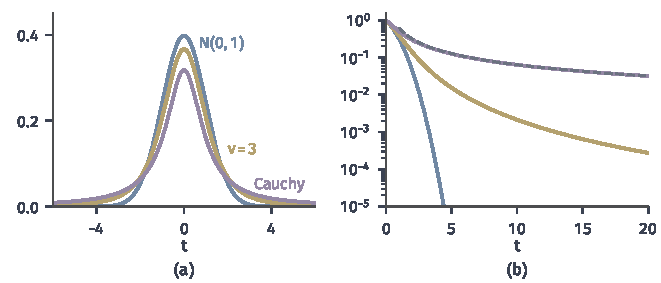
\includegraphics[width=112mm]{figures/07-probability/01-elementary-probability/matplotlib/rvt-cauchy-t/figure.pdf}
  \caption{比值分布的尾部。(a)标准高斯（蓝）、$\nu=3$的t分布（黄）与Cauchy分布（紫）的密度。(b)双侧尾概率$\mathbb{P}(\lvert T\rvert>t)$，纵轴为对数：高斯尾部（蓝）迅速下降，t分布（黄）与Cauchy分布（紫）分别按$t^{-3}$与$t^{-1}$的阶衰减，灰色虚线为$2/(\pi t)$。}
  \label{fig:rvt-cauchy-t}
\end{BookInlineFigure}


\section{极值与顺序统计量}
\label{sec:rvt-order-statistics}

一台设备由$n$个元件串联而成，任何一个失效设备就停机，寿命是各元件寿命的最小值；若并联，最后一个失效时才停机，寿命是最大值。若关心“第$k$个失效的时刻”，就要把所有寿命排序。这些量都不是光滑的代数运算，但它们的阈值事件很容易写出来。

\paragraph{最大值与最小值}
设$M=\max(X_1,\ldots,X_n)$，$L=\min(X_1,\ldots,X_n)$。最大值不超过$t$，当且仅当每一个都不超过$t$；最小值超过$t$，当且仅当每一个都超过$t$：
\[
 \{M\leq t\}=\bigcap_{i=1}^{n}\{X_i\leq t\},\qquad \{L>t\}=\bigcap_{i=1}^{n}\{X_i>t\} .
\]
所以$F_M(t)$就是联合分布函数在$(t,\ldots,t)$处的值，这一点不需要独立。$X_1,\ldots,X_n$相互独立、分布函数为$F_1,\ldots,F_n$时，交事件的概率分解为乘积：
\begin{equation}
 F_M(t)=\prod_{i=1}^{n}F_i(t),\qquad \mathbb{P}(L>t)=\prod_{i=1}^{n}\bigl(1-F_i(t)\bigr) .
 \label{eq:rvt-max-min}
\end{equation}
没有独立时乘积公式一般不成立。例如$X_2=X_1$时$M=X_1$，$F_M=F_1$，而不是$F_1^2$。

\paragraph{两个例子}
$n$个独立$\operatorname{Unif}(0,1)$的最大值满足$F_M(t)=t^n$，密度$nt^{n-1}$，即$\operatorname{Beta}(n,1)$。$n=2$时$\mathbb{P}(M\leq0.5)=0.25$：图~\ref{fig:rvt-max-min-events}(a)中，$M\leq t$的原像是边长为$t$的小正方形，$L>t$的原像是右上角边长为$1-t$的正方形。

独立的指数寿命$X_i\sim\operatorname{Exp}(\lambda_i)$串联时，由式~\eqref{eq:rvt-max-min}，
\[
 \mathbb{P}(L>t)=\prod_{i=1}^{n}\mathrm{e}^{-\lambda_it}=\mathrm{e}^{-(\lambda_1+\cdots+\lambda_n)t},
\]
所以$L\sim\operatorname{Exp}(\lambda_1+\cdots+\lambda_n)$：失效率相加。取$\lambda=(1,2,3)$，串联寿命服从$\operatorname{Exp}(6)$，均值$1/6$。

还可以问哪个元件最先失效。$X_1$最先失效，即$X_1<\min(X_2,X_3)$；后者服从$\operatorname{Exp}(5)$，且与$X_1$独立。对$X_1$的取值积分，得到
\[
 \mathbb{P}(X_1<\min(X_2,X_3))=\int_0^\infty\mathrm{e}^{-t}\cdot\mathrm{e}^{-5t}\,\mathrm{d}t=\frac16 .
\]
一般地，第$i$个最先失效的概率是$\lambda_i/\sum_j\lambda_j$。

\paragraph{离散情形}
两枚骰子的较大点数$M$，由式~\eqref{eq:rvt-max-min}，$F_M(m)=(m/6)^2$，于是
\begin{equation}
 \mathbb{P}(M=m)=\frac{m^2-(m-1)^2}{36}=\frac{2m-1}{36},\qquad m=1,\ldots,6 .
 \label{eq:rvt-dice-max}
\end{equation}
图~\ref{fig:rvt-max-min-events}(b)中，$M=m$的原像是一个L形，由$m$个横格与$m$个竖格组成，拐角的格子$(m,m)$被两边共用，所以是$2m-1$格而不是$2m$格。这个拐角在后面讨论同值时还会出现。

\begin{BookInlineFigure}
  \centering
  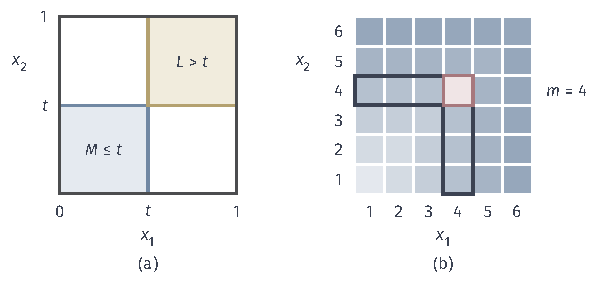
\includegraphics[width=101.3mm]{figures/07-probability/01-elementary-probability/tikz/rvt-max-min-events/figure.pdf}
  \caption{极值事件的原像。(a)单位正方形中，浅蓝正方形是$\max(X_1,X_2)\leq t$，浅黄正方形是$\min(X_1,X_2)>t$，这里$t=0.5$。(b)两枚骰子，同一种蓝色深浅的L形格子较大点数相同，红色格子是$M=m$的L形拐角$(m,m)$，以$m=4$为例共$7$格。}
  \label{fig:rvt-max-min-events}
\end{BookInlineFigure}

\paragraph{顺序统计量}
把$X_1,\ldots,X_n$从小到大排列，记为$X_{(1)}\leq X_{(2)}\leq\cdots\leq X_{(n)}$，$X_{(k)}$称为第$k$个\term{顺序统计量}（order statistic）。$X_{(1)}=L$，$X_{(n)}=M$；$n$为奇数时$X_{((n+1)/2)}$是中间的那个值。

设$X_1,\ldots,X_n$独立同分布，分布函数为$F$。求$X_{(k)}$的分布，关键是把阈值事件改写成计数：$X_{(k)}\leq t$当且仅当至少有$k$个$X_i$不超过$t$。记$N_t$为不超过$t$的个数，它是$n$个示性变量$\mathbf{1}_{\{X_i\leq t\}}$之和。由定理~\ref{thm:rvt-group-independence}，这些示性变量独立，各自以概率$F(t)$取$1$，所以$N_t\sim\operatorname{Bin}(n,F(t))$。

有密度时还可以先看一个直观的计数。$X_{(k)}$落在$[t,t+\Delta t]$，大致意味着：有$k-1$个落在$t$左边，一个落在这一小段里，$n-k$个落在右边。选出这三组的方法有$n!/((k-1)!\,1!\,(n-k)!)$种，每种的概率约为$F(t)^{k-1}\cdot f(t)\Delta t\cdot(1-F(t))^{n-k}$。下面的定理把这个计数严格化。

\begin{theorem}[顺序统计量的分布]
\label{thm:rvt-order-statistics}
设$X_1,\ldots,X_n$独立同分布，分布函数为$F$。
\begin{enumerate}
 \item 对任意$t$与$1\leq k\leq n$，
 \begin{equation}
  \mathbb{P}(X_{(k)}\leq t)=\sum_{j=k}^{n}\binom{n}{j}F(t)^{j}\bigl(1-F(t)\bigr)^{n-j} .
  \label{eq:rvt-order-cdf}
 \end{equation}
 \item 若$F$有密度$f$，则在$f$的连续点处
 \begin{equation}
  f_{X_{(k)}}(t)=\frac{n!}{(k-1)!\,(n-k)!}F(t)^{k-1}\bigl(1-F(t)\bigr)^{n-k}f(t) .
  \label{eq:rvt-order-density}
 \end{equation}
 \item 若$F$有密度$f$，则$(X_{(1)},\ldots,X_{(n)})$有联合密度
 \begin{equation}
  f_{(1),\ldots,(n)}(x_1,\ldots,x_n)=n!\,\prod_{i=1}^{n}f(x_i),\qquad x_1<x_2<\cdots<x_n ,
  \label{eq:rvt-order-joint}
 \end{equation}
 在其他地方为零。
\end{enumerate}
\end{theorem}

\begin{proof}
第一条：$X_{(k)}\leq t$与$N_t\geq k$是同一个事件，而$N_t\sim\operatorname{Bin}(n,F(t))$，把二项质量从$j=k$加到$n$即可。这一步没有用到密度，对含原子的分布同样成立。

第二条：在$f$的连续点处$F'=f$，对式~\eqref{eq:rvt-order-cdf}逐项求导。记$p=F(t)$，第$j$项的导数是
\[
 \binom{n}{j}\Bigl(jp^{j-1}(1-p)^{n-j}-(n-j)p^{j}(1-p)^{n-j-1}\Bigr)f(t) .
\]
利用$\binom{n}{j}j=n\binom{n-1}{j-1}$与$\binom{n}{j}(n-j)=n\binom{n-1}{j}$，并记$a_j=\binom{n-1}{j}p^{j}(1-p)^{n-1-j}$（$a_n=0$），第$j$项化为$nf(t)(a_{j-1}-a_j)$。从$j=k$加到$n$，中间各项相消，只剩
\[
 nf(t)\,a_{k-1}=n\binom{n-1}{k-1}p^{k-1}(1-p)^{n-k}f(t) ,
\]
系数$n\binom{n-1}{k-1}=n!/((k-1)!(n-k)!)$，即式~\eqref{eq:rvt-order-density}。

第三条：排序映射把$\mathbb{R}^{n}$映到$\{x_1<\cdots<x_n\}$。去掉某两个坐标相等的点组成的集合（体积为零）之后，$\mathbb{R}^{n}$按坐标的相对次序分成$n!$个开区域，每个区域上排序映射是一个坐标置换，Jacobian行列式的绝对值为$1$。由式~\eqref{eq:rvt-multivariate-branch}，$n!$个分支各贡献$\prod_if(x_{\pi(i)})$，而乘积与次序无关，都等于$\prod_if(x_i)$，合计$n!\prod_if(x_i)$。
\end{proof}

第三条在$n=2$时就是第~\ref{sec:rvt-branches-reduction}节的排序例子。系数$n!$说明排序把$n!$种次序的质量折叠到同一个有序区域里，这与绝对值变换把两个半轴的质量对折到一起是同一件事。

\paragraph{均匀样本}
$X_i\sim\operatorname{Unif}(0,1)$时$F(t)=t$，$f=1$，式~\eqref{eq:rvt-order-density}成为
\[
 f_{U_{(k)}}(t)=\frac{n!}{(k-1)!\,(n-k)!}t^{k-1}(1-t)^{n-k},\qquad 0<t<1 ,
\]
即$U_{(k)}\sim\operatorname{Beta}(k,n-k+1)$，均值$k/(n+1)$。$n$个点把$[0,1]$分成$n+1$段，由对称性每段的平均长度都是$1/(n+1)$，第$k$个点的平均位置就是$k/(n+1)$。

取$n=3$、$k=2$，三个均匀数的中间值的密度是$6t(1-t)$。由式~\eqref{eq:rvt-order-cdf}，
\[
 \mathbb{P}(U_{(2)}\leq0.25)=3\cdot0.25^2\cdot0.75+0.25^3=0.140625+0.015625=0.15625 .
\]
对密度积分也得到同一个值：
\[
 \int_0^{0.25}6t(1-t)\,\mathrm{d}t=3\cdot0.25^2-2\cdot0.25^3=0.15625 .
\]图~\ref{fig:rvt-order-stats}画出$n=5$时五个顺序统计量的密度。

\begin{BookInlineFigure}
  \centering
  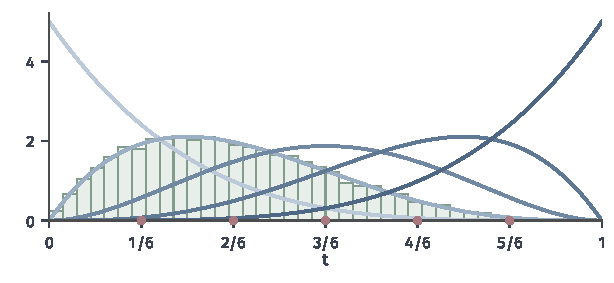
\includegraphics[width=104mm]{figures/07-probability/01-elementary-probability/matplotlib/rvt-order-stats/figure.pdf}
  \caption{$n=5$个独立$\operatorname{Unif}(0,1)$的顺序统计量。蓝色由浅到深是$U_{(1)},\ldots,U_{(5)}$的密度$\operatorname{Beta}(k,6-k)$，红点标出均值$k/6$；浅绿直方图是$20000$组模拟样本中$U_{(2)}$的值（种子$19$）。}
  \label{fig:rvt-order-stats}
\end{BookInlineFigure}

\paragraph{同值与原子}
式~\eqref{eq:rvt-order-density}与式~\eqref{eq:rvt-order-joint}依赖一件事：样本两两不同的概率为$1$，这样$n!$种次序互不重叠。分布有原子时，同值出现的概率为正，两枚骰子点数相同的概率就是$1/6$，这时按$n!$个分支计数会重复计算。

骰子的最大值说明了这一点。若仿照式~\eqref{eq:rvt-order-density}，用$2F(m)p(m)$代替$\mathbb{P}(M=m)$，得到$2m/36$，对$m$求和是
\[
 \sum_{m=1}^{6}\frac{2m}{36}=\frac{42}{36}>1 .
\]
多出的$6/36$恰好是六个对角格子$(m,m)$：它们在“第一枚最大”与“第二枚最大”两个分支中各被算了一次。正确的计数是式~\eqref{eq:rvt-dice-max}的$2m-1$。

有原子时应回到式~\eqref{eq:rvt-order-cdf}，它只用了计数$N_t$，对任何分布都成立。离散变量的质量由分布函数的跳跃得到：记$F(t^-)=\mathbb{P}(X<t)$，把式~\eqref{eq:rvt-order-cdf}中的$F(t)$换成$F(t^-)$就得到$\mathbb{P}(X_{(k)}<t)$，两者相减就是$\mathbb{P}(X_{(k)}=t)$。

以三枚骰子的中间点数为例，求它等于$3$的概率。$F(3)=1/2$，$F(3^-)=F(2)=1/3$，代入式~\eqref{eq:rvt-order-cdf}，
\[
 \mathbb{P}(X_{(2)}\leq3)=3\cdot\frac14\cdot\frac12+\frac18=\frac12,\qquad \mathbb{P}(X_{(2)}<3)=3\cdot\frac19\cdot\frac23+\frac1{27}=\frac{7}{27} .
\]
两者之差是$\mathbb{P}(X_{(2)}=3)=1/2-7/27=13/54\approx0.241$，直接枚举$216$种结果也得到$52$种，即$52/216=13/54$。


\section{本章小结}
\label{sec:rvt-summary}

本章回答的问题是：输入的规律已知、输出由确定的公式算出时，输出服从什么分布。所有计算都从原像规则~\eqref{eq:rvt-preimage-rule}出发：把关于输出的事件写回输入空间，用输入的质量表或联合密度计算。离散时这就是把被送到同一点的质量相加；连续时先得到分布函数，需要密度时再把积分换到输出的坐标上。

换坐标时，记录伸缩的因子各不相同，但道理一样：概率不变，所占的长度或体积变了，密度就按比例反向调整。下表把本章的公式放在一起，最后一列是各自新增的检查。

\begin{BookInlineTable}
  \centering
  \small
  \begin{tabular}{@{}lll@{}}
    \toprule
    映射 & 密度公式 & 须检查的条件 \\
    \midrule
    一元单调 & $f_X(h(y))\lvert h'(y)\rvert$ & 不等号方向、$g'\neq0$、支撑 \\
    一元多分支 & 各逆像贡献之和 & 每支单调、漏支、原子 \\
    同维可逆 & $f_{\bm{X}}(\bm{h}(\bm{y}))\lvert\det D\bm{h}(\bm{y})\rvert$ & 一一、行列式非零、取值区域 \\
    降维 & 补坐标后积掉 & 补出的变换可逆 \\
    和 & $\int f_{X,Y}(x,z-x)\,\mathrm{d}x$ & 独立时才成为卷积 \\
    乘积 & $\int f_{X,Y}(x,z/x)\lvert x\rvert^{-1}\,\mathrm{d}x$ & 零处的原子另计 \\
    比值 & $\int f_{X,Y}(rw,w)\lvert w\rvert\,\mathrm{d}w$ & 分母不取零，尾部与矩 \\
    排序 & $n!\prod_if(x_i)$ & 同值概率为零，否则用计数式 \\
    \bottomrule
  \end{tabular}
  \caption{本章的变换公式与各自的条件。}
  \label{tab:rvt-summary}
\end{BookInlineTable}

几条共同的教训贯穿各节。第一，分布与少数数值特征不同：期望与方差由边缘和协方差决定，完整的输出分布却需要联合规律。第~\ref{sec:rvt-output-distribution}节的三张概率表、第~\ref{sec:rvt-difference-distribution}节的三种依赖都说明了这一点。第二，独立是卷积、封闭性和乘积分解的前提，不能换成“不相关”或“边缘同族”；独立的分组经变换后仍然独立，读同一组输入的两个量则通常不独立。

第三，退化情形要单独处理。导数在一段区间上为零会产生原子，奇异的线性映射使支撑降维，输入在零处的原子会传给乘积，有原子的样本会出现同值。第四，分母靠近零是比值重尾的来源：均匀变量之比与Cauchy分布的均值都不存在，t分布的$k$阶矩存在当且仅当$k<\nu$。

本章顺带补全了前几章留下的几处推导：多元高斯的满维密度来自线性换元，$\chi^2_1$来自平方变换，Rayleigh分布与均匀方向角来自极坐标，Gamma归一化同时给出Dirichlet密度与总量的独立性，t分布来自高斯与$\chi^2$变量之比。

这些计算都把输出的分布写成“输入分布在映射下的像”。第~\ref{chap:probability-spaces}章将在一般的概率空间上统一这种“像分布”：原像规则成为它的定义，本章各种公式成为它在具体映射下的计算，离散、连续与混合的情形也不再分开处理。另一方面，本章的许多变换可以反过来用：$-\ln U$把均匀变量变成指数变量，极坐标把均匀角度和Rayleigh半径变成一对独立高斯，第~\ref{chap:sample-generation}章将利用这些变换从均匀随机数生成指定分布的样本。


